% Mobile-C Library 

%%%%%%%%%%%%%%%%%%%%%%%%%%%%%%%%%%%%%%%%%%%%%%%%%%%%%%%%%%%%%%%%%%%%%%
% Preamble {{{
%\documentclass[11pt]{article}
\documentclass[11pt]{report}
\usepackage{varioref}
\usepackage{times,here,verbatim,fancyheadings,makeidx}
%\usepackage{psfig}
\usepackage[pdftex]{hyperref}
\usepackage{hypcap}
\usepackage{fullpage}
\usepackage{amssymb,amsmath}
\usepackage{graphicx}
\usepackage{program}
\headrulewidth 0.0pt
\hoffset=-0.0625in
%\voffset=0pt
\setlength{\textheight}{9in}
\setlength{\textwidth}{6.5in}
\topmargin=0.05in
\makeindex
% }}} Preamble
%%%%%%%%%%%%%%%%%%%%%%%%%%%%%%%%%%%%%%%%%%%%%%%%%%%%%%%%%%%%%%%%%%%%%%

%%%%%%%%%%%%%%%%%%%%%%%%%%%%%%%%%%%%%%%%%%%%%%%%%%%%%%%%%%%%%%%%%%%%%%
% Title Page {{{
\begin{document}
\thispagestyle{empty}
\begin{center}

\includegraphics[width=1.8in]{figure/mobilec_logo.png}


\vspace{0.5in}
{\Huge\sf\bf Mobile-C} \\
\vspace{0.1in}
{\LARGE\sf\bf -- A Multi-Agent Platform for Mobile C/C++ Agents} \\
\vspace{0.4in}
{\LARGE\sf\bf User's Guide} \\
\vspace{0.4in}
{\LARGE\sf\bf Version 2.0.6} \\
\vspace{1.0in}
{\Large\sf\bf Harry H. Cheng} \\
\vspace{1.0in}
{\large\sf\bf Mobile-C User's Guide version 2.0.6 prepared by:} \\
\vspace{0.2in}
David Ko\\
Harry H. Cheng
\vspace{1in}

\vspace{2.0in}
{\large\sf\bf\today}
%September 20, 2007
\end{center}

%%%%%%%%%%%%%%%%%%%%%%%%%%%%%%%%%%%%%%%%%%%%%%%%%%%%%%%%%%%%%%%%%%%%%%
% Contributors {{{
%\phantomsection
%\addcontentsline{toc}{chapter}{Major contributors}
\pagebreak
\noindent
{\LARGE\sf\bf Major Contributors (in alphabetical order)} \\
{\small
\verbatiminput{../AUTHORS}
}
% }}} Contributors 
%%%%%%%%%%%%%%%%%%%%%%%%%%%%%%%%%%%%%%%%%%%%%%%%%%%%%%%%%%%%%%%%%%%%%%
\pagebreak


%%%%%%%%%%%%%%%%%%%%%%%%%%%%%%%%%%%%%%%%%%%%%%%%%%%%%%%%%%%%%%%%%%%%%%
% Copyright {{{
\thispagestyle{empty}
%\phantomsection
%\addcontentsline{toc}{chapter}{Copyright}
\noindent
{\Large\bf Copyright}\\
\verbatiminput{../Copyright}
% }}} Copyright 
%%%%%%%%%%%%%%%%%%%%%%%%%%%%%%%%%%%%%%%%%%%%%%%%%%%%%%%%%%%%%%%%%%%%%%

\pagebreak
% }}} Title Page
%%%%%%%%%%%%%%%%%%%%%%%%%%%%%%%%%%%%%%%%%%%%%%%%%%%%%%%%%%%%%%%%%%%%%%

%%%%%%%%%%%%%%%%%%%%%%%%%%%%%%%%%%%%%%%%%%%%%%%%%%%%%%%%%%%%%%%%%%%%%%
% Abstract {{{
%\phantomsection
%\addcontentsline{toc}{chapter}{Abstract}
\begin{abstract} 
Mobile-C is an IEEE FIPA (Foundation for Intelligent Physical Agents) standard 
compliant multi-agent platform for supporting C/C++ mobile agents in networked 
intelligent mechatronic and embedded systems. Although it is a general-purpose 
multi-agent platform, Mobile-C is specifically designed for real-time and 
resource constrained applications with interface to hardware. Mobile agents 
are software components that are able to move between different execution 
environments. Mobile agents in a multi-agent system communicate and work 
collaboratively with other agents to achieve a global goal. It allows a 
mechatronic or embedded system to adapt to a dynamically changing environment.

\vspace{1in}
%%%%%%%%%%%%%%%%%%%% begin figure %%%%%%%%%%%%%%%%%%%% 
%\begin{figure}[H]
\centerline{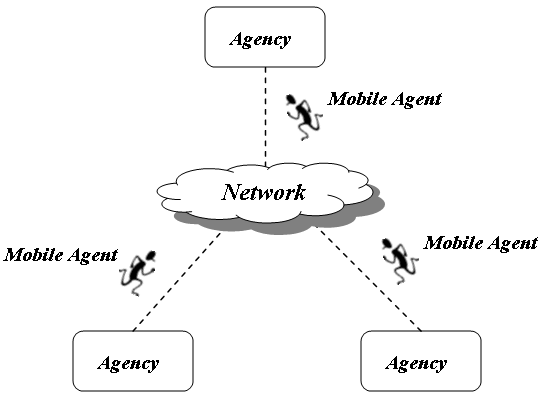
\includegraphics[scale=0.6]{figure/coverfigure}}
%\end{figure}
%%%%%%%%%%%%%%%%%%%% end figure %%%%%%%%%%%%%%%%%%%%%%
\end{abstract}
\pagebreak
% Abstract }}}
%%%%%%%%%%%%%%%%%%%%%%%%%%%%%%%%%%%%%%%%%%%%%%%%%%%%%%%%%%%%%%%%%%%%%%

%%%%%%%%%%%%%%%%%%%%%%%%%%%%%%%%%%%%%%%%%%%%%%%%%%%%%%%%%%%%%%%%%%%%%%
% Table of Contents {{{
\pagenumbering{roman}
\setcounter{page}{1}
\tableofcontents
\pagebreak
% }}} Table of Contents
%%%%%%%%%%%%%%%%%%%%%%%%%%%%%%%%%%%%%%%%%%%%%%%%%%%%%%%%%%%%%%%%%%%%%%

%%%%%%%%%%%%%%%%%%%%%%%%%%%%%%%%%%%%%%%%%%%%%%%%%%%%%%%%%%%%%%%%%%%%%%
% Part 1 {{{
\pagenumbering{arabic}
\setcounter{page}{1}
\pagebreak
% }}} Part 1 
%%%%%%%%%%%%%%%%%%%%%%%%%%%%%%%%%%%%%%%%%%%%%%%%%%%%%%%%%%%%%%%%%%%%%%

%%%%%%%%%%%%%%%%%%%%%%%%%%%%%%%%%%%%%%%%%%%%%%%%%%%%%%%%%%%%%%%%%%%%%%
% Introduction {{{
%\pagenumbering{arabic}
%\setcounter{page}{1}
%\pagestyle{fancy}
\chapter{Introduction}
Parallel and distributed computing~\cite{Kumar}~\cite{Manber} are widely used 
in scientific and engineering fields, especially for time-critical or 
time-consuming tasks.
Parallel computing is typically carried out in dedicated multiprocessors with
a central clock and shared memory.
On the other hand, distributed computing is decentralized parallel
computing, using two or more computers communicating over a network to
accomplish a common objective or task.
It is similar to computer clustering with the main difference being a wide
geographic dispersion of the resources.
In addition to the main difference, the types of hardware, programming 
languages, operating systems and other resources may vary drastically as well 
in distributed computing.

Although the processing speed of networked computers is typically not as fast 
as that of a dedicated parallel computer, networked computers are less
expensive and more broadly available.
Due to the rapid improvement in network hardware and software that makes
distributed computing faster, more broadly available, and easier-to-implement
than before, there are more and more research investigations nowadays 
targeting or exploiting this low-end, decentralized parallel computing.
Meanwhile, as the scale of distributed applications rapidly expands, 
there is an increasing demand for the code mobility.

Agent technology can significantly enhance the design and analysis of 
problem domains under the following three conditions~\cite{Adler}: 
(1) the problem domain is geographically distributed; 
(2) the subsystems exist in a dynamic environment; 
(3) the subsystems need to interact with each other more flexibly. 
Mobile agents are software components that can travel between 
different execution environments~\cite{Fuggetta}. 
Mobile agents can be created dynamically during runtime and dispatched to 
source systems to perform tasks with the most updated code. 
Therefore, the mobility of mobile agents provides distributed 
applications with significant flexibility and adaptability which are both 
essential to satisfy the dynamically changing requirements and conditions in 
a distributed environment.

Most of the mobile agent systems were developed to support only Java mobile 
agents.
Furthermore, many of them are standalone platforms. 
In other words, they were not designed to be embedded in a user application 
to support code mobility.  
Mobile-C~\cite{Chenthesis}~\cite{Chen3}~\cite{Mobile-C}~\cite{mobilec_webpage} 
was originally developed as a standalone, IEEE Foundation for Intelligent 
Physical Agents (FIPA) compliant mobile agent platform with a primary 
intention to fit applications where low-level hardware gets involved, such as 
networked mechatronic and embedded systems. 
Since most of these systems are written in C/C++, Mobile-C uses C/C++ as 
the mobile agent language for easy interfacing with control programs and 
underlying hardware. 
In addition, Mobile-C uses an embeddable C/C++ interpreter -- Ch, originally 
developed by Cheng~\cite{SP1}~\cite{CUJ1}~\cite{Ch}, to support the execution 
of C/C++ mobile agent code. 

In order to provide distributed applications with code mobility, this 
user's guide presents a mobile agent library, the Mobile-C library. 
The Mobile-C library is supported in various operating systems including 
Windows, Unix, and real-time OS.
It has a small footprint to satisfy the small memory requirement for a 
variety of mechatronic and embedded systems. 
This mobile agent library allows Mobile-C to be embedded in a program to 
support C/C++ mobile agents.
The API functions in this library facilitate the development of a multi-agent
system that can easily interface with a variety of hardware devices. 
%\pagebreak
% }}} Introduction
%%%%%%%%%%%%%%%%%%%%%%%%%%%%%%%%%%%%%%%%%%%%%%%%%%%%%%%%%%%%%%%%%%%%%%

%%%%%%%%%%%%%%%%%%%%%%%%%%%%%%%%%%%%%%%%%%%%%%%%%%%%%%%%%%%%%%%%%%%%%%
% Mobile-C Library Installation {{{
\chapter{Mobile-C Library Installation}
This chapter describes the prerequisites to install the Mobile-C library and 
the installation steps for both Unix and Windows operating systems.

%%%%%%%%%%%%%%%%%%%%%%%%%%%%%%%%%%%%%%%%%%%%%%%%%%%%%%%%%%%%%%%%%%%%%%
% SUB: Requirements {{{
\section{Requirements}
This user's guide assumes all necessary software packages are installed
correctly and function. 
The software packages required to successfully install the Mobile-C library 
include:

\noindent
(1) Ch version 6.3.0 or greater: It can be obtained from http://www.softintegration.com

\noindent
(2) Embedded Ch version 6.3.0 or greater: It can be obtained from http://www.softintegration.com

% }}} SUB: Prerequisites 
%%%%%%%%%%%%%%%%%%%%%%%%%%%%%%%%%%%%%%%%%%%%%%%%%%%%%%%%%%%%%%%%%%%%%%

%%%%%%%%%%%%%%%%%%%%%%%%%%%%%%%%%%%%%%%%%%%%%%%%%%%%%%%%%%%%%%%%%%%%%%
% SUB: Installation on Unix {{{
\section{Installation on Unix}

\subsection{Install the Mobile-C library}
The following commands will install the Mobile-C library in the system 
directory for {\bf 32-bit} Unix systems. 
The system directory for Unix systems is usually `/usr/local/lib' or 
  `/usr/lib' depending on your system.

\begin{verbatim}
    cd <MCPACKAGE>/src
    ./configure
    make
    make install
\end{verbatim}

The following commands will install the Mobile-C library in the system 
  directory for {\bf 64-bit} Unix systems. 
The only difference between the above and below commands is that `fPIC' is 
  added into CFLAGS for compilation.

\begin{verbatim}
    cd <MCPACKAGE>/src
    ./configure CFLAGS=-fPIC
    make
    make install
\end{verbatim}

By default, the Mobile-C library created contains both shared and static 
versions, which are `libmc.so.0.0.0' and `libmc.a', respectively.
The header file, libmc.h, used in the C/C++ binary 
space will be placed in the system directory, which is usually 
`usr/local/include' or `/usr/include' depending on your system.
 
Note that these commands will automatically build mxml-2.2.2 and
xyssl-0.7, both of which are packaged with Mobile-C, but will
not install these libraries. The Mobile-C libraries only need
these libraries to compile, but does not need them installed in
order to run.

Also note that the above commands will automatically compile all the included
demos automatically after compiling the Mobile-C library. The demos will
run even if the 'make install' step is omitted.

The `--prefix' option can be used to specify the home directory to 
install the Mobile-C files, as shown in the following commands.

\begin{verbatim}
    cd <MCPACKAGE>/src
    ./configure --prefix=<MCHOME>
    make
    make install
\end{verbatim}

\noindent
\texttt{<MCPACKAGE>} is the directory created by unpacking the Mobile-C compressed 
tar file.
\texttt{<MCHOME>} is the installation directory for the Mobile-C library and 
header file.\\
\noindent
The library files `libmc.so.0.0.0' and `libmc.a' will be installed in 
\texttt{<MCHOME>/lib}, and the header file `libmc.h' will be placed in 
\texttt{<MCHOME>/include}.

% }}} SUB: Installation on Unix
%%%%%%%%%%%%%%%%%%%%%%%%%%%%%%%%%%%%%%%%%%%%%%%%%%%%%%%%%%%%%%%%%%%%%%

%%%%%%%%%%%%%%%%%%%%%%%%%%%%%%%%%%%%%%%%%%%%%%%%%%%%%%%%%%%%%%%%%%%%%%
% SUB: Installation on Windows {{{
\section{Installation on Windows}
\subsection{Building the Mobile-C Library}
The following steps are suggested to build the Mobile-C library.
\begin{enumerate}
\item Ensure that your \texttt{\_chrc} file in your home directory is up to
  date. The \texttt{\_chrc} file may be opened from the ChIDE text editor by
  opening ChIDE, selecting "Options" from the menu, and selecting the "Open
  Local Ch Startup File" menu item. The section in your \texttt{\_chrc} file
  which contains settings about
  your Visual C++ installation must be correct. 
\item Unpack the Mobile-C source code. Ensure that you have write permissions
  for the directory you are unpacking Mobile-C into, or you may encounter 
  compile-time errors. As mentioned in the previous section, we will refer
  to the unpacked directory as \texttt{<MCPACKAGE>}.
\item Open a Ch terminal.
\item Navigate to the \texttt{<MCPACKAGE>} directory in your Ch terminal. For
  example, if you unpacked Mobile-C to the \texttt{C:$\backslash$Mobile-C} directory, type
  \texttt{cd C:$\backslash$Mobile-C} in your Ch terminal.
\item Type the command \texttt{nmake -f makefile.win32} to build the Mobile-C
  library, as well as all of the demos in the \texttt{<MCPACKAGE>/demos/}
  directory.
\end{enumerate}
% }}} SUB: Installation on Windows 
%%%%%%%%%%%%%%%%%%%%%%%%%%%%%%%%%%%%%%%%%%%%%%%%%%%%%%%%%%%%%%%%%%%%%%

%%%%%%%%%%%%%%%%%%%%%%%%%%%%%%%%%%%%%%%%%%%%%%%%%%%%%%%%%%%%%%%%%%%%%%
% SUB: Installation on KoreBot {{{
\section{Installation on KoreBot}

\subsection{Build the Mobile-C library}
A bash script, \textit{build\_korebot}, is used to build the Mobile-C library 
and an executable sample program, \textit{mc\_sample\_app}, for KoreBot board.

Running the script will create a directory called \textit{korebot\_mc} that 
contains \textit{bin}, \textit{include} and \textit{lib} directories.
\textit{bin} directory contains the executable sample program.    
\textit{include} directory contains the header file \textit{libmc.h}.
\textit{lib} directory contains the Mobile-C related static and shared 
libraries.

Two paths, \textit{KOREBOT\_CHHOME} and \textit{KOREBOT\_TOOLCHAINHOME}, 
in the bash script might need to be changed to match the correct 
paths set up in a user's system.
\textit{KOREBOT\_CHHOME} is the directory containing Ch files built for 
KoreBot board.
\textit{KOREBOT\_TOOLCHAINHOME} is the directory containing cross compiler 
related files for KoreBot board. 

Use the following commands to run the bash script.

\begin{verbatim}
    cd <MCPACKAGE>
    ./build_korebot
\end{verbatim}
% }}} SUB: Installation on KoreBot 
%%%%%%%%%%%%%%%%%%%%%%%%%%%%%%%%%%%%%%%%%%%%%%%%%%%%%%%%%%%%%%%%%%%%%%

%%%%%%%%%%%%%%%%%%%%%%%%%%%%%%%%%%%%%%%%%%%%%%%%%%%%%%%%%%%%%%%%%%%%%%
% SUB: Installation on Gumstix {{{
\section{Installation on Gumstix}

\subsection{Build the Mobile-C library}
A bash script, \textit{build\_gumstix}, is used to build the Mobile-C library 
and an executable sample program, \textit{mc\_sample\_app}, for Gumstix 
computer.

Running the script will create a directory called \textit{gumstix\_mc} that 
contains \textit{bin}, \textit{include} and \textit{lib} directories.
\textit{bin} directory contains the executable sample program.    
\textit{include} directory contains the header file \textit{libmc.h}.
\textit{lib} directory contains the Mobile-C related static and shared 
libraries.

Two paths, \textit{GUMSTIX\_CHHOME} and \textit{GUMSTIX\_TOOLCHAINHOME}, 
in the bash script might need to be changed to match the correct 
paths set up in a user's system.
\textit{GUMSTIX\_CHHOME} is the directory containing Ch files built for 
Gumstix computer. By default, it is set to the value \texttt{/usr/local/gumstix\_ch/ch/}.
\textit{GUMSTIX\_TOOLCHAINHOME} is the directory containing cross compiler 
related files for Gumstix computer. By default, it is set to the value \texttt{/usr/local/gumstix-buildroot}.

Use the following commands to run the bash script.

\begin{verbatim}
    cd <MCPACKAGE>
    ./build_gumstix
\end{verbatim}
% }}} SUB: Installation on Gumstix 
%%%%%%%%%%%%%%%%%%%%%%%%%%%%%%%%%%%%%%%%%%%%%%%%%%%%%%%%%%%%%%%%%%%%%%

%%%%%%%%%%%%%%%%%%%%%%%%%%%%%%%%%%%%%%%%%%%%%%%%%%%%%%%%%%%%%%%%%%%%%%
% Installing the Mobile-C Ch Package{{{
\section{Installing the Mobile-C Ch Package}
The Mobile-C Ch Package will be required if agents need to use any of the
Mobile-C FIPA ACL message functions, such as \texttt{mc\_AclSend()} or
\texttt{mc\_AclRetrieve()}. To install the Mobile-C Ch package, please follow
these steps:
\begin{enumerate}
\item From the Mobile-C root directory, run the command: \\
\texttt{ch ./pkgcreate.ch} \\
This will create a directory called ``\texttt{chmobilec}''.
\item From within a Ch shell, run the command: \\
\texttt{sudo pkginstall.ch chmobilec} \\
If you are using Microsoft Windows, you may omit the "\texttt{sudo}" part of the
command which is required on unix-like systems to ensure proper installation
permassions.
\end{enumerate}
% }}} Installing the Mobile-C Security Module
%%%%%%%%%%%%%%%%%%%%%%%%%%%%%%%%%%%%%%%%%%%%%%%%%%%%%%%%%%%%%%%%%%%%%%

\section{Creating your own compilation environment}
If a custom build environment is required, there are several directories which
must be added to the search paths for header files and libraries. There are 
also a variety of system libraries which Mobile-C must be linked with in order
to compile properly.

\subsection{UNIX and Mac systems}
In order to compile properly, the extra include directory
\texttt{<CHHOME>/extern/include} must be added to the default include search
directories. The directory \texttt{<CHHOME>/extern/lib} must also be added to
the list of searched library directories. Furthermore, the following libraries
must be linked with Mobile-C during the link step:
\begin{itemize}
\item libmxml (Provided with Mobile-C in the directory \texttt{<MCHOME>/src/mxml/})
\item libmc\_list (Provided with Mobile-C in the directory \texttt{<MCCHOME>/src/mc\_list})
\item libmc\_sync (Provided with Mobile-C in the directory \texttt{<MCCHOME>/src/mc\_sync})
\item libdl
\item libpthread
\item libm
\item libcrypt
\item libembedch (Provided with Embedded-Ch)
\end{itemize}

\subsection{Windows}
For windows, the include directory \texttt{<CHHOME>/extern/include} must be added
to the include paths and the directory \texttt{<CHHOME>/extern/lib} must be added
to the library search paths. Furthermore, the library \texttt{wsock32.lib} must
be linked with Mobile-C in order to compile properly.

% }}} Mobile-C Library Installation 
%%%%%%%%%%%%%%%%%%%%%%%%%%%%%%%%%%%%%%%%%%%%%%%%%%%%%%%%%%%%%%%%%%%%%%

%%%%%%%%%%%%%%%%%%%%%%%%%%%%%%%%%%%%%%%%%%%%%%%%%%%%%%%%%%%%%%%%%%%%%%
% Getting Started{{{
\chapter{Getting Started}
%%%%%%%%%%%%%%%%%%%%%%%%%%%%%%%%%%%%%%%%%%%%%%%%%%%%%%%%%%%%%%%%%%%%%%
% SUB: Compilation on Unix{{{
\section{Compilation on Unix}
All the demo programs are compiled automatically in the Unix version.
% }}} Compilation on Unix
%%%%%%%%%%%%%%%%%%%%%%%%%%%%%%%%%%%%%%%%%%%%%%%%%%%%%%%%%%%%%%%%%%%%%%

%%%%%%%%%%%%%%%%%%%%%%%%%%%%%%%%%%%%%%%%%%%%%%%%%%%%%%%%%%%%%%%%%%%%%%
% SUB: Compilation on Windows{{{
\section{Compilation on Windows}
All the demo programs are compiled automatically in the Windows version. Single
demos may be recompiled by navigating to a demo directory in a Ch terminal with
the \texttt{cd} and \texttt{ls} commands, and then executing the commands
\texttt{nmake -f makefile.win32} to compile a demo, or \texttt{nmake -f
makefile.win32 clean} to delete all compiled files.
% }}} SUB: Compilation on Windows 
%%%%%%%%%%%%%%%%%%%%%%%%%%%%%%%%%%%%%%%%%%%%%%%%%%%%%%%%%%%%%%%%%%%%%%

%%%%%%%%%%%%%%%%%%%%%%%%%%%%%%%%%%%%%%%%%%%%%%%%%%%%%%%%%%%%%%%%%%%%%%
% SUB: Overview of Sample Application Programs {{{
\section{Overview of Sample Application Programs}
%%%%%%%%%%%%%%%%%%%%%%%%%%%%%%%%%%%%%%%%%%%%%%%%%%%%%%%%%%%%%%%%%%%%%%
% Program: server.c {{{
\begin{Program}[!h]
\capstart
\begin{center}
   {\footnotesize \linespread{1.0} \verbatiminput{../demos/getting_started/hello_world/server.c}}
\end{center}
\caption{A sample Mobile-C server. (demos/getting\_started/hello\_world/server.c)}
\label{prog:server.c}
\end{Program}
% }}} Program: server.c
%%%%%%%%%%%%%%%%%%%%%%%%%%%%%%%%%%%%%%%%%%%%%%%%%%%%%%%%%%%%%%%%%%%%%%

%%%%%%%%%%%%%%%%%%%%%%%%%%%%%%%%%%%%%%%%%%%%%%%%%%%%%%%%%%%%%%%%%%%%%%
% Program: client.c {{{
\begin{Program}%[!h]
\capstart
\begin{center}
   {\footnotesize \linespread{1.0} \verbatiminput{../demos/getting_started/hello_world/client.c}}
\end{center}
\caption{A sample Mobile-C client program. The sole purpose of this program is to
  send a Mobile-C agent to another agency. (demos/getting\_started/hello\_world/client.c)}
\label{prog:client.c}
\end{Program}
% }}} Program: client.c
%%%%%%%%%%%%%%%%%%%%%%%%%%%%%%%%%%%%%%%%%%%%%%%%%%%%%%%%%%%%%%%%%%%%%%


Program \vref{prog:server.c} starts an agency that is capable of 
receiving mobile agents and executing mobile agent code. 

{\footnotesize \linespread{1.0} \verbatiminput{../demos/getting_started/hello_world/server.c.1}}
\noindent
The header file {\bf libmc.h} is included at the beginning of the program. 
It defines all the data types, macros and function prototypes for the 
Mobile-C library.

{\footnotesize \linespread{1.0} \verbatiminput{../demos/getting_started/hello_world/server.c.2}}
\noindent
The variable $agency$, of type {\bf MCAgency\_t}, is a handle that contains 
information of an agency. The second line initializes a local variable that will
hold the port number we wish the agency to bind to.

{\footnotesize \linespread{1.0} \verbatiminput{../demos/getting_started/hello_world/server.c.3}}
\noindent
{\bf MC\_Initialize()} \index{MC\_Initialize()} takes an integer and the address of an 
{\bf MCAgencyOptions\_t} \index{MCAgencyOptions\_t} variable as its two parameters. 
An {\bf MCAgencyOptions\_t} variable is a structure that contains 
information about which threads to be activated and the default agent 
status specified by a user.
Here, a {\bf NULL} pointer is passed to {\bf MC\_Initialize()} as the second 
parameter instead of an MCAgencyOptions\_t variable to start an agency with 
default settings. 
A local agency will be initialized to listen on port {\bf 5051} specified by 
the variable $local\_port$.

{\footnotesize \linespread{1.0} \verbatiminput{../demos/getting_started/hello_world/server.c.4}}
\noindent
The agency waits indefinitely for a mobile agent by the function 
{\bf MC\_MainLoop()} \index{MC\_MainLoop()}. 

Program \ref{prog:client.c} starts an agency that sends a mobile agent to 
a remote agency.
Examining Programs \ref{prog:server.c} and \ref{prog:client.c}, we see
that there are only two new API function calls:
\begin{verbatim}
  agent = MC_ComposeAgentFromFile(
      "mobagent1",      /* Name */
      "localhost:5050", /* Home */
      "IEL",            /* Owner */
      "hello_world.c",  /* Filename */
      NULL,             /* Return var name. NULL for no return */
      "localhost:5051", /* Server to execute task on */
      0 );              /* Persistent. 0 for no persistence. */
\end{verbatim}
and
\begin{verbatim}
  MC_AddAgent(agency, agent);
\end{verbatim}

Mobile-C agents may be created from existing source code files. The example
above takes a source code file called \texttt{hello\_world.c} and constructs
an agent around it. The agent's name, home, owner, return variable name,
and the host on which to execute the agent are all provided as arguments
to the \texttt{MC\_ComposeAgentFromFile()} function. 

Then, the newly created agent is added to the local agency so that it may
perform its local and/or remote tasks. In our example, the agent has
one remote task, so the agent will migrate to the remote host and perform
its task there. 

Also note that any valid hostname may be used in place of ``localhost''. The
communicating agencies need not be on the same physical machine; in fact, in most
cases they will be on seperate machines. Any IPv4 string, i.e. ``169.237.104.199'', or
qualified hostname, i.e. ``machine.ucdavis.edu'', may be used. For instance, the
code
\begin{verbatim}
    MC_ComposeAgentFromFile(
                "Bob",
                "iel.ucdavis.edu:5050",
                "IEL",
                "source_code.c",
                "169.237.104.199:5055",
                NULL,
                0);
\end{verbatim}
will send an agent to the server at address ``169.237.104.199'' listening on
port 5055. Or,
\begin{verbatim}
    MC_ComposeAgentFromFile(
                "Lou",
                "iel.ucdavis.edu:5055",
                "IEL",
                "agent_source.c",
                "machine.ucdavis.edu:5031",
                NULL,
                0);
\end{verbatim}
will send the agent to an agency at ``machine.ucdavis.edu'' listening on 
port 5031.
% }}} SUB: Overview of Sample Application Programs
%%%%%%%%%%%%%%%%%%%%%%%%%%%%%%%%%%%%%%%%%%%%%%%%%%%%%%%%%%%%%%%%%%%%%%

%%%%%%%%%%%%%%%%%%%%%%%%%%%%%%%%%%%%%%%%%%%%%%%%%%%%%%%%%%%%%%%%%%%%%%
% SUB: Mobile-C Bluetooth Agencies {{{
\section{Mobile-C Bluetooth Agencies (Experimental)}
As of Mobile-C version 2.0.2, Mobile-C has support for using Bluetooth
as the agent message transport medium as opposed to the standard TCP/IP.
A new option has been added to the \texttt{MCAgencyOptions\_t} structure
to indicate whether or not Mobile-C should start as a Bluetooth enabled
agency.

Please note that currently, Mobile-C is unable to start as both a Bluetooth
agency and a standard TCP/IP agency. That is, if a Mobile-C agency is
initialized to communicate via Bluetooth, that same agency will not be able to
communicate via TCP/IP, and vise versa. 

When Mobile-C is initialized as a Bluetooth agency, it enables Mobile-C to
send and receive messages to other Mobile-C Bluetooth agencies, via the
short/medium range Bluetooth wireless protocol. A sample Mobile-C 
server program that listens for incoming connections is shown below.

{\footnotesize \linespread{1.0} \verbatiminput{../demos/getting_started/bluetooth/server.c}}

Note that this program is very similar to the previous ``hello world''
server.c, seen at Program \ref{prog:server.c}. One major difference to take
note is the line which reads

\begin{verbatim}
options.bluetooth = 1;
\end{verbatim}

This line sets the option in the Mobile-C options structure to inform Mobile-C
to initialize as a Bluetooth agency.

Also note the initializing port number. Bluetooth RFCOMM port numbers are
limited to values from 0 to 30. The value  ``20'' was chosen arbitrarily, but
it must lie between zero and thirty. 

The client program, which sends an agent to the server agency, is also similar
to the previous client program seen at Program \ref{prog:client.c}.

{\footnotesize \linespread{1.0} \verbatiminput{../demos/getting_started/bluetooth/client.c}}

Note that the hostname supplied to the \texttt{MC\_ComposeAgentFromFile()}
function is composed of the MAC address of the server Bluetooth device,
followed by a space, followed by the port the server agency is listening on.

% }}} SUB: Mobile-C Bluetooth Agencies
%%%%%%%%%%%%%%%%%%%%%%%%%%%%%%%%%%%%%%%%%%%%%%%%%%%%%%%%%%%%%%%%%%%%%%

%%%%%%%%%%%%%%%%%%%%%%%%%%%%%%%%%%%%%%%%%%%%%%%%%%%%%%%%%%%%%%%%%%%%%%
% SUB: Execution of Sample Applications {{{
\section{Execution of Sample Applications}
In general, each of the demos is designed to have very similar execution
procedures. For each demo, there are one or more ``servers'', which are
simply vanilla Mobile-C agencies. To run the demo, start all of the servers
(there is only one server for most of the demos), and start the ``client''
program. Generally, the client program also starts a Mobile-C agency,
but it typically sends an agent to a destination as part of its startup
process as well.

For example, to run the Mobile-C ``Hello World'' example, 
run the following commands from a text terminal on the server machine
to start an agency listening on port {\bf 5051}.

\begin{verbatim}
    cd <MCPACKAGE>/demos/hello_world
    ./server
\end{verbatim}

\noindent
Next, run the following commands from a text terminal on the client machine
to start an agency listening on 
port {\bf 5050} and send the mobile agent to the remote agency 
listening on port {\bf 5051}.\\

\begin{verbatim}
    cd <MCPACKAGE>/demos/hello_world
    ./client
\end{verbatim}

\noindent
After the mobile agent message is received and the mobile agent code is 
executed, the string {\bf Hello World!} should be printed to the text terminal 
on the server machine. Note that in this example, both the server and client
are running on the same machine, but this is not a requirement. The field
``localhost'' may be replaced with any qualified domain name or IP address. 


% }}} Execution of Sample Applications
%%%%%%%%%%%%%%%%%%%%%%%%%%%%%%%%%%%%%%%%%%%%%%%%%%%%%%%%%%%%%%%%%%%%%%

%%%%%%%%%%%%%%%%%%%%%%%%%%%%%%%%%%%%%%%%%%%%%%%%%%%%%%%%%%%%%%%%%%%%%%
% The Mobile-C Library {{{
\section{The Mobile-C Library}
The Mobile-C library allows a Mobile-C agency to be embedded in a program to 
support C/C++ mobile agents.
In addition, the Mobile-C API gives users a full control over a Mobile-C 
agency embedded in a program. 
Therefore, the Mobile-C library not only provides a significant code mobility 
for distributed applications, but also facilitates the development of a 
multi-agent system that can easily interface with various hardware devices. 

%%%%%%%%%%%%%%%%%%%%%%%%%%%%%%%%%%%%%%%%%%%%%%%%%%%%%%%%%%%%%%%%%%%%%%
% FIGURE {{{ 
\begin{figure*}[!t]
\begin{center}
   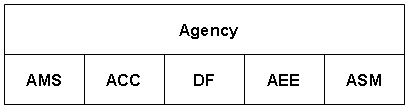
\includegraphics[scale=0.5]{figure/mobilec_lib_arch}
   \caption{Architecture of the Mobile-C library.}
   \label{fig:mobilec_lib_arch}
\end{center}
\end{figure*}
% FIGURE }}} 
%%%%%%%%%%%%%%%%%%%%%%%%%%%%%%%%%%%%%%%%%%%%%%%%%%%%%%%%%%%%%%%%%%%%%%

%%%%%%%%%%%%%%%%%%%%%%%%%%%%%%%%%%%%%%%%%%%%%%%%%%%%%%%%%%%%%%%%%%%%%%
% FIGURE {{{ 
\begin{figure*}[!t]
\begin{center}
   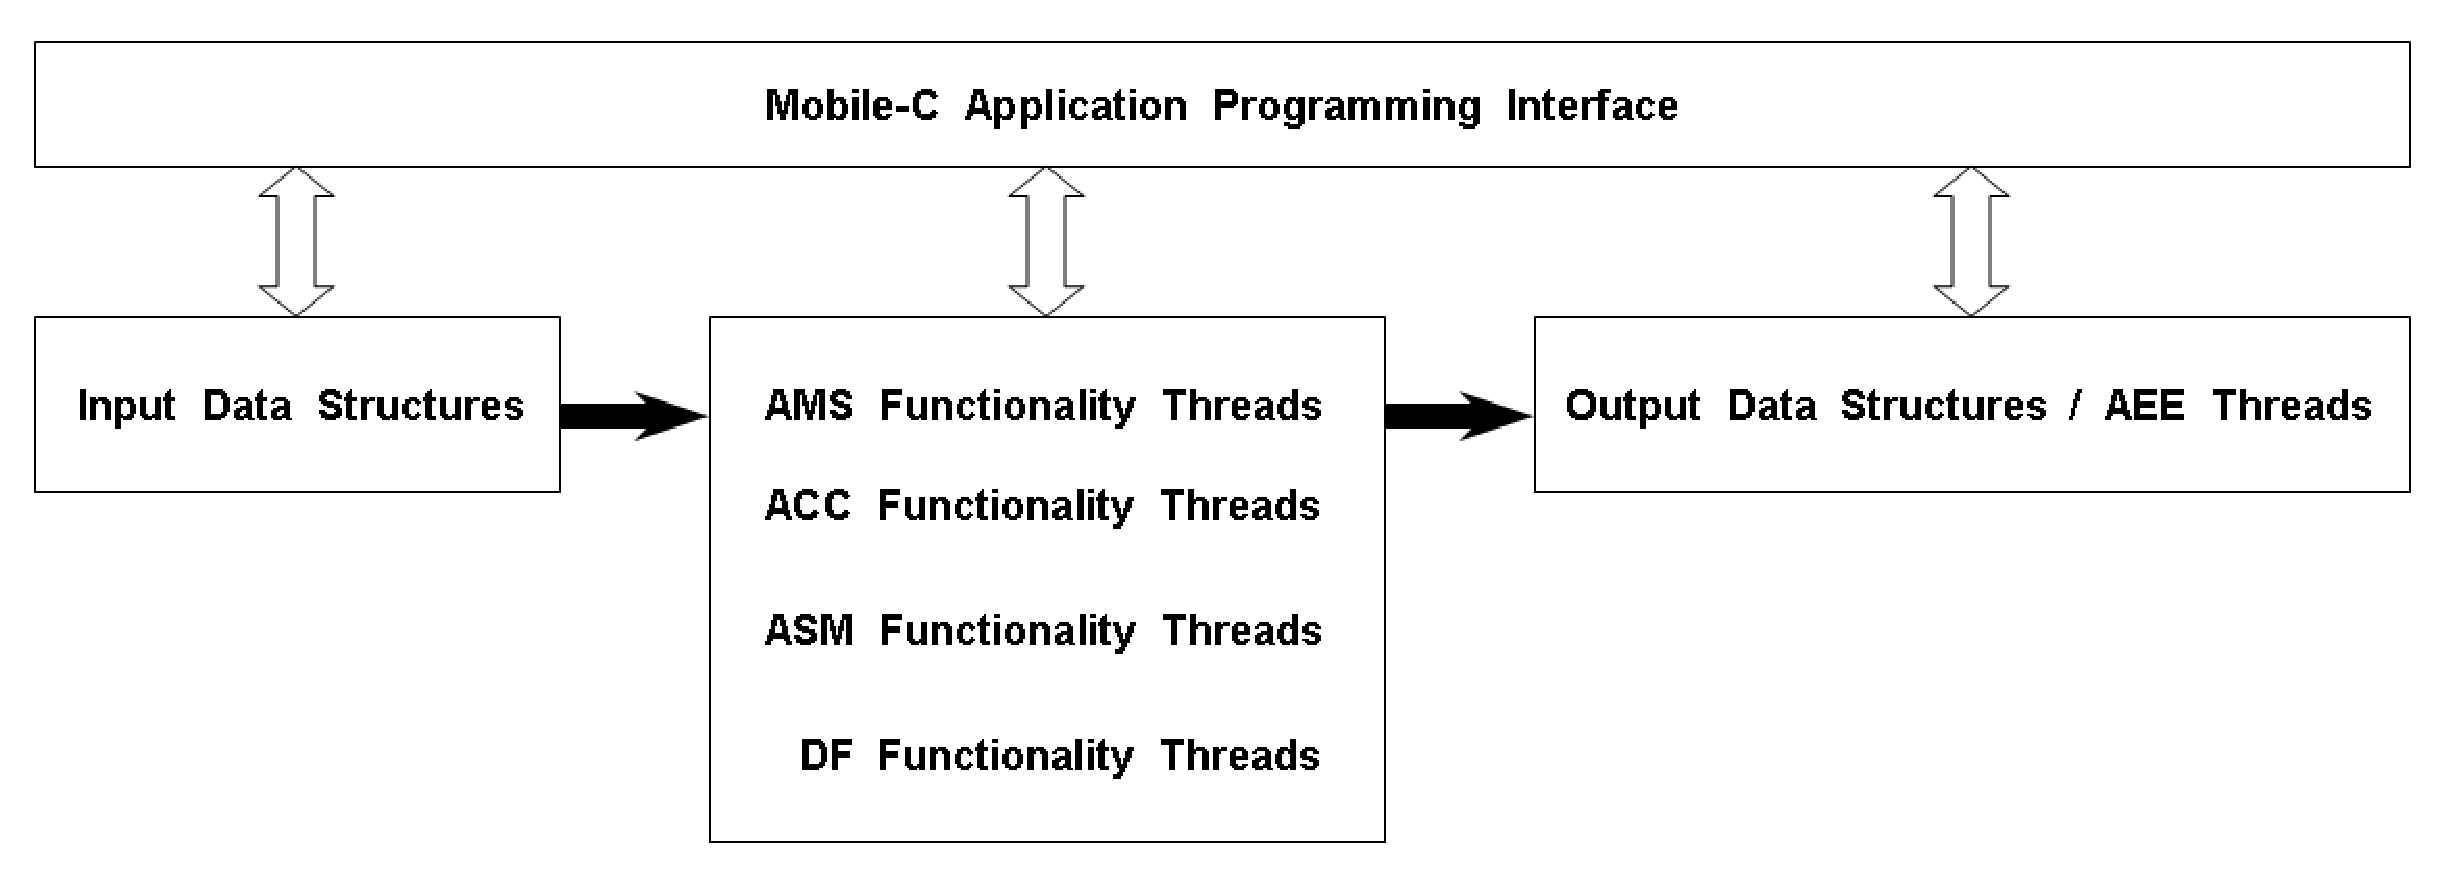
\includegraphics[scale=0.5]{figure/mobilec_lib_imp}
   \caption{Implementation overview of the Mobile-C library.}
   \label{fig:mobilec_lib_imp}
\end{center}
\end{figure*}
% FIGURE }}} 
%%%%%%%%%%%%%%%%%%%%%%%%%%%%%%%%%%%%%%%%%%%%%%%%%%%%%%%%%%%%%%%%%%%%%%

%%%%%%%%%%%%%%%%%%%%%%%%%%%%%%%%%%%%%%%%%%%%%%%%%%%%%%%%%%%%%%%%%%%%%%
% Architecture of the Mobile-C Library {{{
\subsection{Architecture of the Mobile-C Library \label{mobilec_arch}}
Figure \ref{fig:mobilec_lib_arch} illustrates the architecture of the 
Mobile-C library.
The Mobile-C library allows a Mobile-C agency to be embedded in a program to 
support C/C++ mobile agents.
A Mobile-C agency refers to a mobile agent platform within which mobile agents 
exist and operate.
The Mobile-C API gives users a full control over a Mobile-C agency and its 
different modules.
 
As a IEEE FIPA compliant mobile agent platform, a Mobile-C agency 
comprises three FIPA normative modules, Agent Management System (AMS), 
Agent Communication Channel (ACC) and Directory Facilitator (DF). 
Two additional modules, Agent Execution Engine (AEE) and 
Agent Security Manager (ASM), are included in a Mobile-C agency as well.
These modules provide different functionalities summarized as follows.

\textit{Agent Management System (AMS)}

\noindent
An AMS controls the creation, registration, execution, migration, 
persistence, and termination of a mobile agent. 
It maintains a directory of Agent Identifiers (AIDs) for registered mobile 
agents. 
Each mobile agent must register with an AMS in order to have a valid AID.

\textit{Agent Communication Channel (ACC)}

\noindent
An ACC routes messages between local and remote entities. 
It is responsible for the interactions between distributed components, such 
as inter-agent communication and inter-platform agent transport. 
The interactions can be performed through Agent Communication Language (ACL) 
message exchange.

\textit{Directory Facilitator (DF)}

\noindent
A DF serves yellow page services. 
Mobile agents wishing to advertise their services should register with a DF. 
Visiting mobile agents can search a DF for mobile agents providing the 
services they desire.

\textit{Agent Execution Engine (AEE)}

\noindent
An AEE serves as the execution environment for mobile agent code.
An AEE has to be platform independent in order to support the execution of 
mobile agents in a heterogeneous environment. 

Each AEE contains an Embedded Ch interpreter to interpret the agent C code.
By default, the agency will preload four interpreters upon startup for
interpreting agents. If more than four interpreters are required, the agency
will dynamically allocate extra interpreters as needed. See the reference for
\texttt{MC\_Initialize()} on page \pageref{api:MC_Initialize} for more info.

\textit{Agent Security Manager (ASM)}

\noindent
An ASM is responsible for maintaining securita policies for the host system.
Some sample tasks of an ASM include identifying users, protecting host 
resources, authenticating and authorizing mobile agents, and ensuring the 
security and integrity of mobile agents.
% }}} Architecture of the Mobile-C Library
%%%%%%%%%%%%%%%%%%%%%%%%%%%%%%%%%%%%%%%%%%%%%%%%%%%%%%%%%%%%%%%%%%%%%%

%%%%%%%%%%%%%%%%%%%%%%%%%%%%%%%%%%%%%%%%%%%%%%%%%%%%%%%%%%%%%%%%%%%%%%
% SUB: Implementation of the Mobile-C Library {{{
\subsection{Implementation of the Mobile-C Library}
Figure \ref{fig:mobilec_lib_imp} shows the implementation overview of the 
Mobile-C library.
The functionalities of each module of an agency are 
implemented as independent threads classified into five categories, that is, 
the AMS functionality threads, the ACC functionality threads, the DF 
functionality threads, the ASM functionality threads and the AEE threads.
Each AEE thread is launched by one of the AMS functionality threads.

The Mobile-C library provides API functions to specify which thread needs to 
be active or inactive when an agency is initialized.
It also provides API functions to access the input and output data structures 
associated with the functionality threads.
A Mobile-C agency maintains a list of synchronization variables that can be 
used with a group of Mobile-C functions to ensure synchronization among 
mobile agents and threads.
The sizes of the Mobile-C static and shared libraries for Linux are about 
500 KB and 390 KB, respectively.

The header file \textit{libmc.h} contains definitions of all the structures and 
functions of the Mobile-C library. 
Table \vref{mobilec_api_cbinary} lists the currently implemented functions 
for the binary space.

% }}} Implementation of the Mobile-C Library
%%%%%%%%%%%%%%%%%%%%%%%%%%%%%%%%%%%%%%%%%%%%%%%%%%%%%%%%%%%%%%%%%%%%%%

% }}} The Mobile-C Library
%%%%%%%%%%%%%%%%%%%%%%%%%%%%%%%%%%%%%%%%%%%%%%%%%%%%%%%%%%%%%%%%%%%%%%

% }}} Getting Started
%%%%%%%%%%%%%%%%%%%%%%%%%%%%%%%%%%%%%%%%%%%%%%%%%%%%%%%%%%%%%%%%%%%%%%

%%%%%%%%%%%%%%%%%%%%%%%%%%%%%%%%%%%%%%%%%%%%%%%%%%%%%%%%%%%%%%%%%%%%%%
% Composing Agents {{{
\chapter{Composing Agents}
Mobile-C agents are represented internally as XML data structures. However,
dealing with XML code requires background knowledge of XML and may be cumbersome.
To enhance the convenience of creating and deploying Mobile-C agents,
several different methods of creating agents from C source code files have
been implemented.

Agents may be composed from plain C source code. There are two main ways to
compose Mobile-C agents. Agents may be composed by using the
\texttt{compose\_send} commmand in the Mobile-C prompt, or by using the
\texttt{MC\_ComposeAgent*} series of API functions.

\section{Mobile-C Command Prompt \texttt{compose\_send} Command}
The \texttt{compose\_agent} takes a C source code file and creates
a fully functioning agent out of it. The \texttt{compose\_send} command
syntax is
\begin{verbatim}
compose_send <filename> <target host> <target port>
\end{verbatim}
Many details about an agent generated in this method, such as the agent's
name and owner, are dynamically generated when creating an agent using 
this method. 
\subsection{Example Execution Using the \texttt{compose\_send} Command}
The demo \texttt{prompt\_example} has been provided with the Mobile-C
package. Note that the source code for both servers is virtually identical to
that in Program \ref{prog:server.c}, except with added execution
instructions.
The demo program is initiated by starting the first agency, named
\texttt{server1}.
\begin{verbatim}
$ ./server1
Agency 1 started. Please start the second agency by running the command
"server2" on another terminal.

MobileC >
\end{verbatim}
Next, the second agency is started on a seperate terminal.
\begin{verbatim}
$ ./server2
Starting Agency...
You may now try the following commands:

  compose_send helloworld.c localhost 5050

The previous command will compose an agent using the source
code in "helloworld.c" and send it to the other agency at
port 5050. Then try this command:

  compose_send helloworld.c localhost 5051

This will send the "hello_world.c" agent to the local agency.
You may also try these commands at the other agency.

MobileC >
\end{verbatim}
Following the instructions on the second agency, we execute the 
suggested \texttt{compose\_send} command. The first agency terminal
now appears as such:
\begin{verbatim}
$ ./server1
Agency 1 started. Please start the second agency by running the command
  "server2" on another terminal.

MobileC > Hello, world!
\end{verbatim}
Note that the source file \texttt{helloworld.c} has been composed into a 
mobile agent, migrated to the \texttt{server1} agency, and executed.

\section{Mobile-C \texttt{MC\_ComposeAgent*} Functions}
There also exist a set of API functions which compose agents from C source
files. These functions are
\begin{itemize}
\item \texttt{MC\_ComposeAgent()} : Compose an agent from program source code. 
\item \texttt{MC\_ComposeAgentWithWorkgroup()} : Compose an agent from program source code with a workgroup code. 
\item \texttt{MC\_ComposeAgentFromFile()} : Compose an agent from a program source code file. 
\item \texttt{MC\_ComposeAgentFromFileWithWorkgroup()} : Compose an agent from a program source code file with a workgroup code. 
\item \texttt{MC\_AgentAddTask()} : Add an additional task to an already formed agent.
\item \texttt{MC\_AgentAddTaskFromFile()} : Add an additional task to an already formed agent from a C source code file.
\end{itemize}
For an example of the usage of these functions, please refer to program
\ref{prog:compose_multi_task_agent}.

\begin{Program}[p]
\begin{center}
   {\footnotesize \linespread{1.0}
     \verbatiminput{../demos/composing_agents/multi_task_example/client_abridged.c}}
\end{center}
\caption{An agency building an agent with multiple tasks from seperate source code files.}
\label{prog:compose_multi_task_agent}
\end{Program}

\section{Agent Workgroups}
In order to provide an added layer of organization and security, agents
may be created which belong to a workgroup. A workgroup's name may be an
ASCII text string of any length. If an agent belongs in a workgroup,
then certain actions on that agent may only be performed by other agents
in the same workgroup. Thus, if a group of agents keeps their workgroup
name private, no agents outside of that group will be able to terminate,
delete, or otherwise affect the agents within the workgroup. All agents are
still able to interact through FIPA ACL messages.

For an example of agent workgroups in action, please see the demo program
in the\\
 \texttt{demos/agent\_workgroup\_example} directory. 
% }}}
%%%%%%%%%%%%%%%%%%%%%%%%%%%%%%%%%%%%%%%%%%%%%%%%%%%%%%%%%%%%%%%%%%%%%%


%%%%%%%%%%%%%%%%%%%%%%%%%%%%%%%%%%%%%%%%%%%%%%%%%%%%%%%%%%%%%%%%%%%%%%
% Agent Data {{{
\chapter{Agent Data}
Agents have the ability to carry pieces of data with them as they migrate from
host to host. The data carried by an agent can be categorized into two broad
types: ``agent return data'' and ``agent saved variables''. 

\section{Agent Return Data}
  ``Agent return data'' is typically used to store a piece of data being
returned to the agent's home agency. For instance, if an agent is given a task
to obtain a single result from a remote host, the agent might store the result
as its agent return data. An agent may hold a single return value for each one
of its tasks. The return value may be of any standard C type, or an array of 
such a type. For instance, the \texttt{double} type, as well as
\texttt{double[5][3]} are both valid types for a piece of agent return data,
since both are examples of a standard C type or an array of a standard type.
User defined structs and unions may not be returned as a piece of return data.
 
In order to return a variable as agent return data, the name of the return variable
simply needs to be specified when composing the agent. No further API calls need to be
executed from within the agent code. Note that the return variable must be declared as
a global variable in the agent code.
For an example of an agent with multiple tasks returning information to its home agency,
please see Program \ref{prog:compose_multi_task_agent} on page
\pageref{prog:compose_multi_task_agent}.

\section{Agent Saved Variables} 
An ``agent saved variable'' is also carried with an agent as it migrates. However,
this type of variable is typically used for data that the agent itself has access
to as it completes its tasks. Furthermore, an agent may save the value of as many
variables as it desires per task. For instance, during an agent's first task, it
may save various values, like the number of other agents on the agency as an
\texttt{int}, and the name of the agency as a \texttt{char[80]}. After it
migrates to it's second task, it may access the variables it saved previously
on the first host. In this way, an agent could calculate the total number of
active agents in an agency network. In summary,

\begin{tabular}{l|cc}
 & Agent Return Data & Agent Saved Variable \\
\hline
May save multiple variables per task & & X \\
\hline
Data easily retrieved by home agency & X & X \\
\hline
Data saved to agent automatically  & & \\
without agent-space API calls & X & \\
\hline
Agent can access its own saved data & & X
\end{tabular}

\vspace{0.18in}
For example, consider an agent with the following tasks. The agent's first task
appears as such:
\verbatiminput{../demos/agent_migration_message_format/agent_saved_variables_example/task1.c}
Note that the variable to be saved must be a global variable. In the agent code, the agent
performs a call to the function \texttt{mc\_AgentVariableSave(mc\_current\_agent, "savevar");}
The first argument in the function is a handle to an agent. The handle \texttt{mc\_current\_agent} is
a special handle an agent has to itself. The second argument is a character string denoting the
name of the variable to save. In effect, this code saves the value of \texttt{savevar} to
itself. As shown in the preceding code, the \texttt{mc\_AgentVariableSave()} function may
be called multiple times on differing variable types and arrays. Each variable will be
saved to the agent prior to migration.

Here is an example of the agent's second task's code:
\verbatiminput{../demos/agent_migration_message_format/agent_saved_variables_example/task2.c}
Note the call to \texttt{mc\_AgentVariableRetrieve(mc\_current\_agent,
"savevar", 0);} in this code example. This function attempts to retrieve a
pointer to the saved variable. The first argument, as seen before, is a handle
to the agent itself. The second variable is the name of the variable to
retrieve. The third argument is the task from which to retrieve the variable,
with the value \texttt{0} being the first task. If the call succeeds, it will
return a valid pointer to the saved variable. If it fails, the function returns
\texttt{NULL}.



% Chapter: Agent Data }}}
%%%%%%%%%%%%%%%%%%%%%%%%%%%%%%%%%%%%%%%%%%%%%%%%%%%%%%%%%%%%%%%%%%%%%%


%%%%%%%%%%%%%%%%%%%%%%%%%%%%%%%%%%%%%%%%%%%%%%%%%%%%%%%%%%%%%%%%%%%%%%
% Mobile-C Agent Migration Message Format {{{
\chapter{Mobile-C Agent Migration Message Format}
\section{General Message Format \label{sec:gen_message_format}}
\begin{Program}
\begin{center}
   {\scriptsize \linespread{1.0} \verbatiminput{../demos/getting_started/hello_world/test1.xml}}
\end{center}
\caption{A rudimentary agent. (demos/getting\_started/hello\_world/test1.xml)}
\label{prog:hello_agent}
\end{Program}
The message format for an agent migration message is designed such that
multiple tasks and multiple code blocks can be migrated from agency to
agency. The message is an XML message with encapsulated C code. An example
of a rudimentary agent can be seen in Program \ref{prog:hello_agent} on 
page \pageref{prog:hello_agent}. 
Following is a brief description of each XML tag.
\begin{itemize}
\item \texttt{MESSAGE}: This tag indicates to Mobile-C that the following data
  is a Mobile-C message. The message type is included in the attribute
  ``message''.
\item \texttt{MOBILE\_AGENT}: This tag indicates that the contained data is a 
  Mobile-C agent.
\item \texttt{AGENT\_DATA}: This tag indicates that the contained data is data pertaining
  to this particular agent.
\item \texttt{NAME}: The name of the agent.
\item \texttt{OWNER}: The owner of the agent. 
\item \texttt{HOME}: The home of the agent. Any agent that has data to ``return'' will
	return it to this address by default.
\item \texttt{WG\_CODE}: The workgroup code of the agent. Workgroup codes are
kept secret by the agent. Only agents with matching workgroup codes are allowed
to perform certain operations on each other, such as agent deletion.
\item \texttt{TASKS}: This indicates that the following information pertains to the
  task or tasks the agent is intended to perform. Attributes found under the
  \texttt{TASKS} tag include:
  \begin{itemize}
    \item \texttt{task} : The total number of tasks the agent has.
    \item \texttt{num} : The task that the agent is currently on.
  \end{itemize}
\item \texttt{TASK}: Each seperate \texttt{TASK} tag indicates a seperate task for the agent
  to perform. The tasks may be seperate hosts and/or code blocks. In the
  rudimentary example, there is only one task. Listed below are the attributes of 
  \texttt{TASK} tags.
  \begin{itemize}
  \item \texttt{num}:           The number of the task. The first task is task number zero.
  \item \texttt{complete}:      Completeness of the task
  \item \texttt{server}:        The host to perform the task
  \item \texttt{return}:        Name of the return variable
  \item \texttt{persistent}:    Persistence of the agent
  \item \texttt{return\_value}: Return value, if not an array
  \item \texttt{code\_id}:      ID of the code block to execute
  \end{itemize}
\textit{complete} and \textit{server} are mandatory attributes, and others are 
optional attributes.  
\item AGENT\_CODE: Each AGENT\_CODE block represents a block of code that 
  the agent may execute. Agents with multiple code blocks may decide at run-time
  which block to execute. Valid attributes under the \texttt{AGENT\_CODE} tag
  include
  \begin{itemize}
    \item \texttt{id}: The id of the code segment, as referenced by the \texttt{TASK} 
      attribute, \texttt{code\_id}.
  \end{itemize}
\end{itemize}

\section{Multiple Tasks with a Single Code Block}
An agent may have an indefinite number of tasks. The agent will perform the tasks
in ther order that they are stated in the XML file, completing each one before
continuing to the next host. Following is an example of an agent which has
multiple tasks to perform, executing the same code block at each new host.
See Program \ref{prog:single_code_block} on page \pageref{prog:single_code_block} 
for an example.
\begin{Program}[p]
\begin{center}
   {\footnotesize \linespread{1.0} 
     \verbatiminput{../demos/composing_agents/multi_task_example/test_single_code_block1.xml}}
\end{center}
\caption{An example agent containing two tasks and a single code block.
  Note that variables ``mc\_host\_name'' and ``mc\_task\_progress'' are special built-in variables described in Table \vref{tab:agent_space_variables}.
  \index{mc\_host\_name}
  \index{mc\_task\_progress}
  \texttt{(<MCPACKAGE>/demos/composing\_agents/multi\_task\_example/test\_single\_code\_block.xml)} }
\label{prog:single_code_block}
\end{Program}
\addtocounter{Program}{-1}
\begin{Program}[p]
\begin{center}
   {\footnotesize \linespread{1.0} 
     \verbatiminput{../demos/composing_agents/multi_task_example/test_single_code_block2.xml}}
\end{center}
\caption{(Continued)}
\end{Program}

\section{Multiple Tasks with Multiple Code Blocks}
See Program \ref{prog:multi_code_block} on page \pageref{prog:multi_code_block}
for a more complicated example of agent code including multiple tasks and
  multiple code blocks. Note that each code block has an associated ID which is 
  refered to in the respective ``DATA'' tags. Also note that more than one ``DATA'' tag
  may refer to the same code block. Thus, an agent may have more ``DATA'' tags than
  code blocks.

\begin{Program}[p]
\begin{center}
   {\footnotesize \linespread{1.0} 
     \verbatiminput{../demos/composing_agents/multi_task_example/test_multi_code_block1.xml}}
\end{center}
\caption{An example agent containing two tasks and two code blocks. 
  \texttt{(<MCPACKAGE>/demos/composing\_agents/multi\_task\_example/test\_multi\_code\_block.xml)}} 
\label{prog:multi_code_block}
\end{Program}
\addtocounter{Program}{-1}
\begin{Program}[p]
\begin{center}
   {\footnotesize \linespread{1.0} 
     \verbatiminput{../demos/composing_agents/multi_task_example/test_multi_code_block2.xml}}
\end{center}
\caption{ (Continued) }
\end{Program}

\section {Multiple Mobile Agent performs Task on Multiple Hosts}
Program \ref{prog:multi_mobile_agent_client} on page \pageref{prog:multi_mobile_agent_client} is a client that sends two different mobile agents to two different hosts. In for loop, it waits for the arrival signal of mobile agent. When an agent arrives it prints the result and delete that agent. For loop is iterated same as total number of mobile agents send by client. The two mobile agents having different name are shown in Program \ref{prog:mobile_agent_1} and Program \ref{prog:mobile_agent_2}:  

\begin{Program}[p]
\begin{center}
   {\footnotesize \linespread{1.0}
     \verbatiminput{../demos/agent_migration_message_format/multi_data_retrieval/client.c}}
\end{center}
\caption{A client program that sends two mobile agents to two different hosts
  \texttt{(<MCPACKAGE>/demos/agent\_migration\_message\_format/multi\_data\_retrieval/client.c)}}
\label{prog:multi_mobile_agent_client}
\end{Program}

\begin{Program}[p]
\begin{center}
   {\footnotesize \linespread{1.0}
     \verbatiminput{../demos/agent_migration_message_format/multi_data_retrieval/test1.xml}}
\end{center}\caption{First mobile agent name "mobagent1" send by client (Program 6) to server 1   
  \texttt{(<MCPACKAGE>/demos/agent\_migration\_message\_format/multi\_data\_retrieval/test1.xml)}}
\label{prog:mobile_agent_1}
\end{Program}

\begin{Program}[p]
\begin{center}
   {\footnotesize \linespread{1.0}
     \verbatiminput{../demos/agent_migration_message_format/multi_data_retrieval/test2.xml}}
\end{center}\caption{Second mobile agent name "mobagent1" send by client (Program 6) to server 2
  \texttt{(<MCPACKAGE>/demos/agent\_migration\_message\_format/multi\_data\_retrieval/test2.xml)}}
\label{prog:mobile_agent_2}
\end{Program}

\section{Agent Return Messages}
If the ``\texttt{name}'' attribute in an agent's ``\texttt{DATA}'' tag
is not set to ``\texttt{no-return}'', the agent will generate an
agent-return message upon completion of all of its tasks. The agent will
generate a return message containing the contents of the variable name
specified in the ``\texttt{name}'' attribute. For instance, Program
\vref{prog:agent_with_return_data} shows a simple agent which 
will migrate to another agency, generate a three-dimensional array called
``\texttt{a}'', and return the contents of the array to the ``\texttt{HOME}''
host upon completion. Note that the return variable must be global
so that the contents are not destroyed upon completion of the \texttt{main}
function. 
  
  An example of the return message that is generated by
this agent can be seen in Program \vref{prog:return_agent}. Notice also in
the return message that the variable type has been changed from ``int'' as it
was in the original program to ``short'' and that the ``\texttt{dim}'' attribute
has been changed to $3$. This is because Mobile-C automatically
checks the type and dimension of the variable it is returning and assign
those attributes automatically.

\begin{Program}[p]
\begin{center}
   {\footnotesize \linespread{1.0} 
     \verbatiminput{../demos/agent_migration_message_format/mc_array_return_example/agent.xml}}
\end{center}
\caption{An agent which returns data upon completion of it's tasks.}
\label{prog:agent_with_return_data}
\end{Program}

\begin{Program}[p]
\begin{center}
   {\footnotesize \linespread{1.0} 
     \verbatiminput{../demos/agent_migration_message_format/mc_array_return_example/return_agent.xml}}
\end{center}
\caption{Agent return data xml format. Note: This XML code has been reformatted
  to a more human-readable format. The actual format generated may differ.}
\label{prog:return_agent}
\end{Program}

\section{Agent Saved Variables}
As of Mobile-C version 1.10.0, Mobile-C agents have the ability to save an 
arbitrary number of variables while migrating from task to task. Agents may
use the agent-space api functions \texttt{mc\_AgentVariableSave()} and
\texttt{mc\_AgentVariableRetrieve} to save and later retrieve variables.
An example agent which does this may be viewed at the documentation for
the \texttt{mc\_AgentVariableSave()} and \linebreak \texttt{mc\_AgentVariableRetrieve()}
functions on pages \pageref{apidoc:mc_AgentVariableSave} and 
\pageref{apidoc:mc_AgentVariableRetrieve}, respectively.

As the agent is migrating from host to host with saved data, the data is 
encapsulated in the agent's XML code. \texttt{<DATA>} tags are created as
children of each \texttt{<TASK>} tag to store data. See Program 
\ref{prog:migrating_agent} for an example of an agent that is migrating
with saved data. The valid attributes within a \texttt{<DATA>} tag are
\begin{itemize}
\item \texttt{name}: The name of the saved variable.
\item \texttt{dim}: The array dimension of the saved variable. 
\item \texttt{type}: The type of the variable.
\item \texttt{value}: (optional) If the variable has zero dimensions, the
  value is stored in this attribute. Otherwise, children \texttt{<ROW>} 
  tags must be created to store the array.
\end{itemize}

Each \texttt{<DATA>} tag may also have children \texttt{<ROW>} tags, if
the data is an array. The valid attributes of the \texttt{<ROW>} tags are
\begin{itemize}
\item \texttt{index}: The index of the row.
\end{itemize}
Note also that each \texttt{<ROW>} tag may contain additional \texttt{<ROW>}
children depending on the dimension of the array being stored.

The Mobile-C XML Data Type Definition (DTD), which defines the format of a
well-formed Mobile-C agent migration message, may be seen in Section
\ref{sec:xml_dtd} on page \pageref{sec:xml_dtd}.

\section{Stationary/Persistent Mobile Agents}
A Stationary agent may be achieved in Mobile-C simply by creating an agent which
never migrates. This is commonly achieved using a couple of different
techniques.
\subsection{An Agent with an Infinite Task}
An agent may be considered stationary if it's task never ends. For instance, if
the task of an agent is of the form:
\begin{verbatim}
while(1)
{
    cmd = wait_for_command();
    execute_command(cmd);
}
\end{verbatim}
Since the previous task never ends, the agent will never terminate and the agent
will remain stationary in it's agency. 

\subsection{The ``\texttt{persistent}'' Agent Flag}
The ``\texttt{persistent}'' flag as mentioned in Section
\ref{sec:gen_message_format} may be used to create a persistent agent. The
example described in Chapter \ref{chap:interface_binary_to_agent} uses such a
technique. This technique creates an agent which is not automatically flushed by the agency
after it completes it's task. Thus, the agent remains dormant and stationary in
the agency without external stimulus.

\begin{Program}[ph]
\begin{center}
{\footnotesize \linespread{1.0}
\verbatiminput{../demos/agent_migration_message_format/agent_saved_variables_example/migrating_agent.xml.part1}}
\end{center}
\caption{\label{prog:migrating_agent} This XML format illustrates an agent which is currently
in the process of migrating with saved data. Note that the agent contains two tasks, and the
first task has been completed. This file is a snapshot of the agent as it is in transit from
task '0' to task '1'. Note the \texttt{<DATA>} tags which store the three variables
referenced by the \texttt{mc\_AgentSaveVariable()} function from within the code, storing
two integers and an integer array. Note that in general, any data type may be stored, including
multi-dimensional arrays.}
\end{Program}
\addtocounter{Program}{-1}
\begin{Program}[ph]
\begin{center}
{\footnotesize \linespread{1.0}
\verbatiminput{../demos/agent_migration_message_format/agent_saved_variables_example/migrating_agent.xml.part2}}
\end{center}
\caption{(Continued)}
\end{Program}


% }}} Mobile-C Agent Migration Message Format
%%%%%%%%%%%%%%%%%%%%%%%%%%%%%%%%%%%%%%%%%%%%%%%%%%%%%%%%%%%%%%%%%%%%%%

%%%%%%%%%%%%%%%%%%%%%%%%%%%%%%%%%%%%%%%%%%%%%%%%%%%%%%%%%%%%%%%%%%%%%%
% {{{ Mobile-C FIPA Compliant ACL Messages
\chapter{Mobile-C FIPA Compliant ACL Messages \label{chap:fipa}}
Mobile-C has the ability to send and receive FIPA compliant
agent communication language (ACL) messages. More information
about FIPA, the Foundation for Intellegent Physical Agents, may be
found at \texttt{http://www.fipa.org}. This functionality allows
Mobile-C agent to communicate with each other, as well as with 
agents from other agencies that are also FIPA compliant. Demos
of communication with JADE agents may be found in the directories
\texttt{<MCPACKAGE>/demos/jade\_to\_mc\_example} and \\
\texttt{<MCPACKAGE>/demos/mc\_to\_jade\_example}.

%{{{ Constructing and Sending an ACL Message
\section{Constructing and Sending an ACL Message}
The general process for constructing an ACL message involves
filling out required portions of an ACL message structure of type
\texttt{struct fipa\_acl\_message\_s} and passing the message to the
\texttt{MC\_AclSend()} function. A number of helper functions 
exist in order to simplify the process of allocating memory and setting
certain fields of the acl message. 
Some typical functions used to compose a new ACL message are the following:
\begin{itemize}
\item \texttt{MC\_AclSetPerformative}: Set the FIPA performative of the message. See Program
  \ref{prog:fipa_enum} for a complete listing of valid FIPA performative enumerations.
\item \texttt{MC\_AclSetSender}: Sets the 'sender' field of the message.
\item \texttt{MC\_AclAddReceiver}: Adds addresses to the 'receiver' field of the message.
\item \texttt{MC\_AclSetContent}: Sets the 'content' field of an ACL message.
\end{itemize}
A detailed example of sending and receiving messages will be presented in
Chapter \ref{chap:stationary_agent}.
%}}}

%{{{Receiving an ACL Message 
\section{Receiving an ACL Message}
Every agent residing on a Mobile-C agency has a mailbox allocated to it.
At any time, the agent may check the mailbox for new ACL messages, or an
agent may choose to wait on an empty mailbox until a new message arrives.
These two tasks are done by the functions \texttt{MC\_AclRetreive()} and
\texttt{MC\_AclWaitRetrieve()}, respectively. 
Another useful function which may be used with a received ACL message is the
\texttt{MC\_AclReply()} function. This function takes an ACL message as an
input argument and automatically forms an ACL reply message addressed to the
original sender. Note that the performative and new sender fields in the reply
message are not automatically initialized and will still need to be set by
the agent. A detailed example of an agent receiving and replying to a message
may be found in Chapter \ref{chap:stationary_agent}.

\begin{Program}[!t]
\begin{center}
   {\footnotesize \linespread{1.0} 
\begin{verbatim}
enum fipa_performative_e
{
  FIPA_ERROR=-1,
  FIPA_ZERO,
  FIPA_ACCEPT_PROPOSAL,
  FIPA_AGREE,
  FIPA_CANCEL,
  FIPA_CALL_FOR_PROPOSAL,
  FIPA_CONFIRM,
  FIPA_DISCONFIRM,
  FIPA_FAILURE,
  FIPA_INFORM,
  FIPA_INFORM_IF,
  FIPA_INFORM_REF,
  FIPA_NOT_UNDERSTOOD,
  FIPA_PROPOGATE,
  FIPA_PROPOSE,
  FIPA_PROXY,
  FIPA_QUERY_IF,
  FIPA_QUERY_REF,
  FIPA_REFUSE,
  FIPA_REJECT_PROPOSAL,
  FIPA_REQUEST,
  FIPA_REQUEST_WHEN,
  FIPA_REQUEST_WHENEVER,
  FIPA_SUBSCRIBE
};
\end{verbatim}
   }
\end{center}
\caption{Fipa Performative Enumerations.}
\label{prog:fipa_enum}
\end{Program}

\pagebreak
\clearpage
\pagebreak
%}}} Section: Receiving an ACL Message

%}}} Chapter: Mobile-C FIPA Compliant ACL Messages
%%%%%%%%%%%%%%%%%%%%%%%%%%%%%%%%%%%%%%%%%%%%%%%%%%%%%%%%%%%%%%%%%%%%%%

%%%%%%%%%%%%%%%%%%%%%%%%%%%%%%%%%%%%%%%%%%%%%%%%%%%%%%%%%%%%%%%%%%%%%%
% Mobile-C Binary Stationary Agents {{{
\chapter{Mobile-C Binary Stationary Agents \label{chap:stationary_agent}}
Mobilec has support for hosting binary-space stationary agents. The
agents are implemented as system threads. As such, the only limit 
to the number of stationary agents residing on an agency are the
system resources of the host agency. 

The binary agents are able to call any of the C-space API functions, such as
\texttt{MC\_AclWaitRetrieve()}. This allows stationary agents to communicate
and interact with other mobile and stationary agents using FIPA ACL messages,
as introduced in Chapter \ref{chap:fipa}.

Stationary agents may be used in any application in which agent mobility is
unnecessary. Stationary agents can typically perform any task a mobile agent
can perform, except migration. Furthermore, stationary agents tend to execute
faster and consume less system resources.

Mobile-C stationary agent threads are added using the
\texttt{MC\_AddStationaryAgent()} API function. See Program 
\ref{prog:stationary_agent_server} for an example of a stationary agent. 

\begin{Program}[!t]
\begin{center}
   {\footnotesize \linespread{1.0} \verbatiminput{../demos/binary_stationary_agents/stationary_agent_communication/server.c}}
\end{center}
\caption{A sample program which starts a single stationary agent that responds to FIPA ACL messages.}
\label{prog:stationary_agent_server}
\end{Program}

The \texttt{MC\_AddStationaryAgent()} function takes three arguments:
\begin{enumerate}
\item A handle to the home agency. This is the agency the new agent will reside under.
\item The agent thread. This is a pointer to a function which will execute and act as
the stationary agent. If the function returns, the stationary agent is terminated.
\item An optional argument to pass to the agent. If additional information or data needs
to be passed to the stationary agent thread, a pointer of any type may be supplied as the
third argument to \\
\texttt{MC\_AddStationaryAgent()}. This pointer may later be retrieved
with the \\
\texttt{MC\_AgentInfo\_GetAgentArgs()} function from within the agent.
\end{enumerate}

The stationary agent thread must have a prototype of the form
\begin{verbatim}
void* agent_func_name(stationary_agent_info_t* agent_info);
\end{verbatim}
As seen in the prototype, the agent thread receives an argument of type
\texttt{stationary\_agent\_info\_t}. This special type is a structure 
which contains information about the the agent, such as its name, and the
location of its mailbox. Certain information may be retrieved from the 
function parameter by using the \texttt{MC\_AgentInfo\_*} series of API
functions, which include:
\begin{itemize}
\item \texttt{MC\_AgentInfo\_GetAgency()} : Retrieves a handle to the host agency.
\item \texttt{MC\_AgentInfo\_GetAgent()} : Retrieves a handle to the agent
information structure.
\item \texttt{MC\_AgentInfo\_GetAgentArgs()} : Retrieves the pointer that was
given as an agent argument during the call to \texttt{MC\_AddStationaryAgent}.
\end{itemize}

Example usage of these functions may be seen in Program \ref{prog:stationary_agent_server}.
%}}}
%%%%%%%%%%%%%%%%%%%%%%%%%%%%%%%%%%%%%%%%%%%%%%%%%%%%%%%%%%%%%%%%%%%%%%

%%%%%%%%%%%%%%%%%%%%%%%%%%%%%%%%%%%%%%%%%%%%%%%%%%%%%%%%%%%%%%%%%%%%%%
% Interface between Binary and Mobile Agent Spaces {{{
\chapter{Interface between Binary and Mobile Agent Spaces
\label{chap:interface_binary_to_agent}}
An embeddable C/C++ interpreter Ch was chosen to be the AEE in the Mobile-C 
library to support C/C++ mobile agents. 
Therefore, in order to access the variables, functions, and data sets in 
the mobile agent space from the binary space, Ch must be first embedded in the 
binary space.
The function \textit{MC\_GetAgentExecEngine()} \index{MC\_GetAgentExecEngine()} in 
Table \ref{mobilec_api_cbinary} returns the AEE associated with a mobile agent 
to the binary space.
Using the AEE returned by \textit{MC\_GetAgentExecEngine()}, all of the 
Embedded Ch functions~\cite{EmbeddedCh} can be called in a binary C/C++ 
program to access the variables, functions, and data sets defined in the 
mobile agent space.
The Embedded Ch toolkit also allows mobile agent code to invoke C/C++ 
functions defined in a binary C/C++ program.

The Embedded Ch toolkit reduces the complexity of heterogeneous development 
environment for both embedded scripting and applications. 
With the consistent C/C++ code base, it can significantly reduce the effort 
in the software development and maintenance. 
Moreover, with the Embedded Ch toolkit, C/C++ applications can be extended 
with all the features of Ch including built-in string type for scripting. 
The Embedded Ch toolkit has a small footprint. 
The pointer and time deterministic nature of the C language provide a 
perfect interface with hardware in real-time systems.

\section{Using an Agent Initialization Callback Function to Intergrate Binary
and Script Space Code}
The user may register a callback function to be called during the initialization
of mobile agents inside of an agency. This allows the user to fine-tune 
an agent and the Ch interpreter before an agent is executed. The callback
function is added using the \texttt{MC\_AddAgentInitCallback()} function,
and the callback function is of the form
\begin{verbatim}
int callback(ChInterp_t interp, MCAgent_t agent, void* user_data);
\end{verbatim}
The user may call any applicable Ch API function on the interpreter,
as well as any applicable Mobile-C API function on the supplied agent.
For instance, the user may use the \texttt{Ch\_DeclareVar()} function
to declare extra variables inside of the interpereter which the agent
will be able to access during its execution. 

The demo located at \texttt{demos/cspace-agentspace\_interface/agent\_init\_callback/} 
provides a demonstration of the callback function. This demo uses the callback
function to declare a new function in each of the incoming agent interpreters
called \texttt{mult()}, which simply multiplies two numbers together. This
means that any incoming agent will be able to call the \texttt{mult()} function,
which resides in C-space, from the agent script-space. This demo may also be seen with
the documentation for \texttt{MC\_AddAgentInitCallback()} on page \pageref{api:MC_AddAgentInitCallback()}.

%%%%%%%%%%%%%%%%%%%%%%%%%%%%%%%%%%%%%%%%%%%%%%%%%%%%%%%%%%%%%%%%%%%%%%
% Invoke a Mobile Agent Space Function from Binary Space {{{
\noindent
\section{Invoke a Mobile Agent Space Function from Binary Space}
%%%%%%%%%%%%%%%%%%%%%%%%%%%%%%%%%%%%%%%%%%%%%%%%%%%%%%%%%%%%%%%%%%%%%%
% client.c {{{
\begin{Program}[!t]
\begin{center}
   {\footnotesize \linespread{1.0} 
     \verbatiminput{../demos/cspace-agentspace_interface/persistent_example/client.c}}
\end{center}
\caption{ A program which sends a persistent mobile agent.
  \texttt{(<MCPACKAGE>/demos/cspace-agentspace\_interface/persistent\_example/client.c)}}
\label{prog:client_ex2.c}
\end{Program}
% }}} client.c
%%%%%%%%%%%%%%%%%%%%%%%%%%%%%%%%%%%%%%%%%%%%%%%%%%%%%%%%%%%%%%%%%%%%%%
%%%%%%%%%%%%%%%%%%%%%%%%%%%%%%%%%%%%%%%%%%%%%%%%%%%%%%%%%%%%%%%%%%%%%%
% test1.xml {{{
\begin{Program}[!t]
\begin{center}
   {\footnotesize \linespread{1.0} 
     \verbatiminput{../demos/cspace-agentspace_interface/persistent_example/test1.xml}}
\end{center}
\caption{A persistent mobile agent. Agents marked ``persistent'' are
  not flushed from the agency after they terminate.
    \texttt{(<MCPACKAGE>/demos/cspace-agentspace\_interface/persistent\_example/test1.xml)}}
\label{prog:mobileagent_ex2.xml}
\end{Program}
% }}} test2.xml
%%%%%%%%%%%%%%%%%%%%%%%%%%%%%%%%%%%%%%%%%%%%%%%%%%%%%%%%%%%%%%%%%%%%%%
%%%%%%%%%%%%%%%%%%%%%%%%%%%%%%%%%%%%%%%%%%%%%%%%%%%%%%%%%%%%%%%%%%%%%%
% host.c {{{
\begin{Program}[!t]
\begin{center}
   {\footnotesize \linespread{1.0} 
     \verbatiminput{../demos/cspace-agentspace_interface/persistent_example/server.c}}
\end{center}
\caption{A Mobile-C agency.
 \texttt{(<MCPACKAGE>/demos/cspace-agentspace\_interface/ persistent\_example/server.c)}}
\label{prog:server_ex2.c}
\end{Program}
% }}} host.c
%%%%%%%%%%%%%%%%%%%%%%%%%%%%%%%%%%%%%%%%%%%%%%%%%%%%%%%%%%%%%%%%%%%%%%
%%%%%%%%%%%%%%%%%%%%%%%%%%%%%%%%%%%%%%%%%%%%%%%%%%%%%%%%%%%%%%%%%%%%%%
% FIGURE {{{
\begin{figure*}[!t]
\begin{center}
   {\footnotesize \linespread{1.0} \verbatiminput{../demos/cspace-agentspace_interface/persistent_example/server_output.txt}}
   \caption{Output from the binary server program.}
   \label{fig:example2_output}
\end{center}
\end{figure*}
% FIGURE }}}
%%%%%%%%%%%%%%%%%%%%%%%%%%%%%%%%%%%%%%%%%%%%%%%%%%%%%%%%%%%%%%%%%%%%%%

This example illustrates how to call a function defined in mobile agent 
code by using the Mobile-C library and Embedded Ch toolkit. 
The mobile agent in this example is a persistent agent, which is not removed 
upon termination of its execution.

The client program shown in Program \vref{prog:client_ex2.c} starts a Mobile-C 
agency listening on port \textit{5050} by the function 
\textit{MC\_Initialize()}, and sends a mobile agent to the remote agency 
running on host \textit{localhost} at port \textit{5051} through 
the function \textit{MC\_SendAgentMigrationMessageFile()}. 
The filename including the full path of the mobile agent is specified from the 
standard input.

The mobile agent sent to the remote agency is 
shown in Program \vref{prog:mobileagent_ex2.xml}. 
The name, owner, source machine of the mobile agent are 
\textit{mobagent1}, \textit{IEL}, and 
\textit{localhost:5050}, respectively. 
The mobile agent is persistent since the flag \textit{persistent}\index{persistent} 
is set to 1 
in Program \ref{prog:mobileagent_ex2.xml}.
This flag can be set to 0 or removed by a user for a non-persistent mobile 
agent.
The embedded mobile agent code is a simple but complete C program which 
defines the function \textit{hello()} to be called in the server program. 

As shown in Program \vref{prog:server_ex2.c}, the server program starts a 
Mobile-C agency listening on port \textit{5051} by the 
function \textit{MC\_Initialize()}, and waits for a mobile agent.  
The mobile agent named \textit{mobagentl} is found by the function 
\textit{MC\_FindAgentByName()} \index{MC\_FindAgentByName()}, and the AEE 
associated with the mobile 
agent is obtained by the function \textit{MC\_AgentExecEngine()} 
\index{MC\_AgentExecEngine()}.
The variable returned by \textit{MC\_AgentExecEngine()} is a Ch interpreter of 
data type \textit{ChInterp\_t}. 
This variable is the first parameter for all of the Embedded Ch functions. 
The function \textit{hello()} defined in the mobile agent code is invoked 
by the Embedded Ch function \textit{Ch\_CallFuncByName()}. 

There are several different methods to call functions in mobile agent 
space from the binary space using the Embedded Ch API. 
Here we describe the function \textit{Ch\_CallFuncByName()}
\index{Ch\_CallFuncByName()} used in Program 
\ref{prog:server_ex2.c}.
With \textit{Ch\_CallFuncByName()}, a function defined in the mobile 
agent space can be called by its name. 
The prototype of \textit{Ch\_CallFuncByName()} is shown as follows.

int Ch\_CallFuncByName(ChInterp\_t interp, char *name, void *retval, ...);

The first argument is an instance of the Ch interpreter. 
The second argument is a string containing the name of the function to be 
called. 
The function name is associated with a function defined in mobile agent code. 
The third argument is a pointer containing the address of the return value of 
the called function. 
If the called function takes any arguments, the arguments should be listed 
after the third argument, \textit{retval}. 
\textit{Ch\_CallFuncByName()} returns zero on successful execution or 
non-zero on failure.

The other method of executing the function is through the Mobile-C
api function {\bf MC\_CallAgentFunc()} \index{MC\_CallAgentFunc()}. 
This method is seen in the example program, Program \ref{prog:server_ex2.c}.

Figure \vref{fig:example2_output} shows the output when the binary file 
\textit{server} compiled from Program \ref{prog:server_ex2.c} was executed. 
The string generated and the value returned from the function \textit{hello()} 
were printed to the screen after the Enter key was pressed once the mobile 
agent had arrived. 

% }}} Invoke a Mobile Agent Space Function from Binary Space 
%%%%%%%%%%%%%%%%%%%%%%%%%%%%%%%%%%%%%%%%%%%%%%%%%%%%%%%%%%%%%%%%%%%%%%

% }}} Interface between Binary and Mobile Agent Spaces
%%%%%%%%%%%%%%%%%%%%%%%%%%%%%%%%%%%%%%%%%%%%%%%%%%%%%%%%%%%%%%%%%%%%%%

%%%%%%%%%%%%%%%%%%%%%%%%%%%%%%%%%%%%%%%%%%%%%%%%%%%%%%%%%%%%%%%%%%%%%%
% Extend Mobile-C Functionality to Mobile Agent Space {{{
\chapter{Extend Mobile-C Functionality to Mobile Agent Space}
%%%%%%%%%%%%%%%%%%%%%%%%%%%%%%%%%%%%%%%%%%%%%%%%%%%%%%%%%%%%%%%%%%%%%%
% FIGURE {{{
\begin{figure*}[b]
\begin{center}
   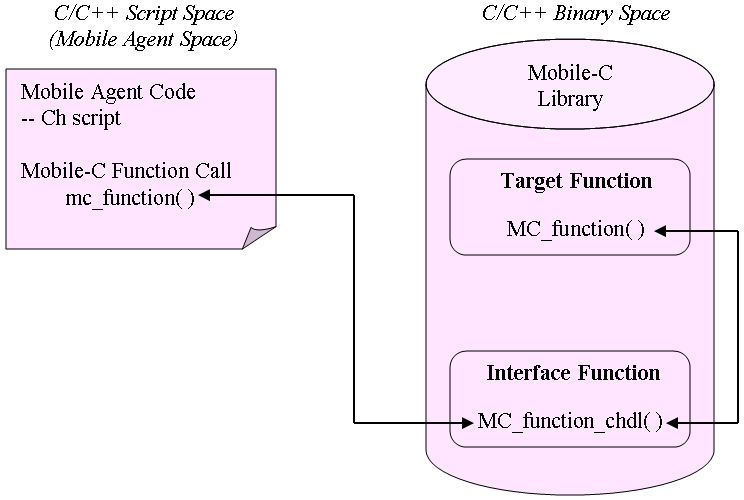
\includegraphics[scale=0.5]{figure/chmobilec_package}
   \caption{Interface of mobile agent code with the Mobile-C library.}
   \label{fig:chmobilec_package}
\end{center}
\end{figure*}
% FIGURE }}}
%%%%%%%%%%%%%%%%%%%%%%%%%%%%%%%%%%%%%%%%%%%%%%%%%%%%%%%%%%%%%%%%%%%%%%
In order to allow mobile agent code to call user defined routines and 
access data sets defined in the binary space, as well as control 
other mobile agents defined in the mobile agent space through the 
Mobile-C API functions, the Mobile-C functionality has to be extended into 
the mobile agent space.
We integrated Ch with the Mobile-C library to provide access to some 
Mobile-C functionalities. 

Figure \vref{fig:chmobilec_package} shows how mobile agent code interfaces 
with the Mobile-C library.
When the function \textit{mc\_function()} is called in mobile agent code,
Ch searches the corresponding interface function \textit{MC\_function\_chdl()} 
in the Mobile-C library, and passes arguments to it by calling the function.
Subsequently, the interface function \textit{MC\_function\_chdl()} invokes the 
target function \textit{MC\_function()}, and passes the return value back to 
the mobile agent space~\cite{EmbeddedCh}.

The prototypes of Mobile-C functions used in the mobile agent space are
declared in \textit{agent.c} through an Embedded Ch function,
\textit{Ch\_DeclareFunc()}.
The data type, \textit{MCAgent\_t}, used as a parameter or return value by 
certain Mobile-C functions for the mobile agent space is also defined in 
\textit{agent.c} by two Embedded Ch functions, 
\textit{Ch\_DeclareVar()} and \textit{Ch\_DeclareTypedef()}~\cite{EmbeddedCh}.
Table \vref{chmobilec_api_cscript} lists the currently implemented functions 
for the mobile agent space.
Two examples are used to demonstrate the applications and features of the 
Mobile-C functionality in the mobile agent space. 

%%%%%%%%%%%%%%%%%%%%%%%%%%%%%%%%%%%%%%%%%%%%%%%%%%%%%%%%%%%%%%%%%%%%%
% Terminate Mobile Agent Execution from Mobile Agent Space {{{
\noindent
\section{Terminate Mobile Agent Execution from Mobile Agent Space}
%%%%%%%%%%%%%%%%%%%%%%%%%%%%%%%%%%%%%%%%%%%%%%%%%%%%%%%%%%%%%%%%%%%%%%
% test2.xml {{{
\begin{Program}[!t]
\begin{center}
   {\footnotesize \linespread{1.0} 
     \verbatiminput{../demos/cspace-agentspace_interface/persistent_example/test2.xml}}
\end{center}
\caption{A mobile agent which enters an infinite loop and does 
  not terminate. \texttt{(<MCPACKAGE>/demos/cspace-agentspace\_interface/persistent\_example/test2.xml)}}
\label{prog:mobileagent1_ex3.xml}
\end{Program}
% }}} test2.xml
%%%%%%%%%%%%%%%%%%%%%%%%%%%%%%%%%%%%%%%%%%%%%%%%%%%%%%%%%%%%%%%%%%%%%%
%%%%%%%%%%%%%%%%%%%%%%%%%%%%%%%%%%%%%%%%%%%%%%%%%%%%%%%%%%%%%%%%%%%%%%
% test3.xml {{{
\begin{Program}[!t]
\begin{center}
   {\footnotesize \linespread{1.0} 
     \verbatiminput{../demos/cspace-agentspace_interface/persistent_example/test3.xml}}
\end{center}
\caption{ This agent terminates the execution
of the agent in Program \ref{prog:mobileagent1_ex3.xml}. 
  \texttt{(<MCPACKAGE>/demos/cspace-agentspace\_interface/persistent\_example/test3.xml)}}
\label{prog:mobileagent2_ex3.xml}
\end{Program}
% }}} test3.xml
%%%%%%%%%%%%%%%%%%%%%%%%%%%%%%%%%%%%%%%%%%%%%%%%%%%%%%%%%%%%%%%%%%%%%%

This example demonstrates how to send a mobile agent to terminate the 
execution of another currently running mobile agent. 
These two mobile agents belong to independent mobile agent spaces. 

The server program used in this example is the same as Program 
\vref{prog:server.c}. 
The client program is the same as Program \vref{prog:client_ex2.c} except 
that it calls the function \textit{MC\_SendAgentMigrationMessageFile()} twice 
to send out two mobile agents.
The first mobile agent sent to the remote agency is 
\textit{test2.xml} shown in Program 
\vref{prog:mobileagent1_ex3.xml}.
The execution of the mobile agent code will repeatedly print a string 
\textit{Hello} to the screen every second.
The second mobile agent sent to the remote agency is 
\textit{test3.xml} shown in Program 
\vref{prog:mobileagent2_ex3.xml}.
The function \textit{mc\_FindAgentByName()} \index{mc\_FindAgentByName()}
returns a variable of type 
\textit{MCAgent\_t} as a handle to a mobile agent. 
The mobile agent code embedded in \textit{mobileagent2\_ex3.xml} finds a 
mobile agent named \textit{mobagent1} by the function 
\textit{mc\_FindAgentByName()} and terminates the execution of 
\textit{mobagent1} by the function \textit{mc\_TerminateAgent()}
\index{mc\_TerminateAgent()}. 
% }}} Terminate Mobile Agent Execution from Mobile Agent Space
%%%%%%%%%%%%%%%%%%%%%%%%%%%%%%%%%%%%%%%%%%%%%%%%%%%%%%%%%%%%%%%%%%%%%%

%%%%%%%%%%%%%%%%%%%%%%%%%%%%%%%%%%%%%%%%%%%%%%%%%%%%%%%%%%%%%%%%%%%%%%
% Invoke a Registered Service from Mobile Agent Space {{{
\noindent
\section{Invoke a Registered Service from Mobile Agent Space}
%%%%%%%%%%%%%%%%%%%%%%%%%%%%%%%%%%%%%%%%%%%%%%%%%%%%%%%%%%%%%%%%%%%%%%
% service_provider_1.xml {{{
\begin{Program}[!t]
\begin{center}
   {\footnotesize \linespread{1.0} 
     \verbatiminput{../demos/agent_space_functionality/mc_df_service_test/service_provider_1.xml}}
\end{center}
\caption{Sample agent containing 'addition' and 'subtraction' services.
Note that the variable ``mc\_current\_agent'' is a special built-in
  variable described in Table
  \vref{tab:agent_space_variables}.\index{mc\_current\_agent}
\texttt{(<MCPACKAGE>/demos/agent\_space\_functionality/mc\_df\_service\_test/ service\_provider\_1.xml)}}
\label{prog:mobileagent1_ex4.xml}
\end{Program}
% }}} service_provider_1.xml
%%%%%%%%%%%%%%%%%%%%%%%%%%%%%%%%%%%%%%%%%%%%%%%%%%%%%%%%%%%%%%%%%%%%%%
%%%%%%%%%%%%%%%%%%%%%%%%%%%%%%%%%%%%%%%%%%%%%%%%%%%%%%%%%%%%%%%%%%%%%%
% service_provider_2.xml {{{
\begin{Program}[!t]
\begin{center}
   {\footnotesize \linespread{1.0} 
     \verbatiminput{../demos/agent_space_functionality/mc_df_service_test/service_provider_2.xml}}
\end{center}
\caption{Sample agent containing 'multiplication' and 'modulus' services.
Note that the variable ``mc\_current\_agent'' is a special built-in
  variable described in Table
  \vref{tab:agent_space_variables}.\index{mc\_current\_agent}
\texttt{(<MCPACKAGE>/demos/mc\_df\_service\_test/service\_provider\_2.xml)}}
\label{prog:mobileagent2_ex4.xml}
\end{Program}
% }}} service_provider_2.xml
%%%%%%%%%%%%%%%%%%%%%%%%%%%%%%%%%%%%%%%%%%%%%%%%%%%%%%%%%%%%%%%%%%%%%%
%%%%%%%%%%%%%%%%%%%%%%%%%%%%%%%%%%%%%%%%%%%%%%%%%%%%%%%%%%%%%%%%%%%%%%
% test2.xml {{{
\begin{Program}[!t]
\begin{center}
   {\scriptsize \linespread{1.0} \verbatiminput{../demos/agent_space_functionality/mc_df_service_test/test1.xml.part1}}
\end{center}
\caption{Sample agent that searches for and invokes agent services.
\texttt{(<MCPACKAGE>/demos/mc\_df\_service\_test/test1.xml)} (Part 1)}
\label{prog:mobileagent3_ex4.xml}
\end{Program}
\addtocounter{Program}{-1}
\begin{Program}[!t]
\begin{center}
   {\scriptsize \linespread{1.0} \verbatiminput{../demos/agent_space_functionality/mc_df_service_test/test1.xml.part2}}
\end{center}
\caption{(Continued) }
\end{Program}
% }}} test2.xml
%%%%%%%%%%%%%%%%%%%%%%%%%%%%%%%%%%%%%%%%%%%%%%%%%%%%%%%%%%%%%%%%%%%%%%

This example demonstrates how to send a mobile agent to invoke a service 
provided by a persistent mobile agent registered with the DF.

The server program used in this example is the same as Program 
\vref{prog:server.c}. 
The client program is the same as Program \vref{prog:client_ex2.c} except 
that it calls the function \textit{MC\_SendAgentMigrationMessageFile()} three
times to send out three mobile agents.
The first mobile agent sent to the remote agency is 
shown in Program 
\vref{prog:mobileagent1_ex4.xml}.
The execution of the mobile agent code will register two services with the 
remote DF through the function mc\_RegisterService(). 
The two services are \textit{addition} and \textit{subtraction} which 
provide addition and subtraction of two integers, respectively.
These services also refer to the functions defined in the mobile agent code.
The function \textit{mc\_RegisterService()} \index{mc\_RegisterService()}
takes three parameters. 
An \textit{MCAgent\_t} type variable is the first parameter. 
A system variable of type \textit{MCAgent\_t}, \textit{mc\_current\_agent}, 
is used as the first parameter when services for 
the current mobile agent are registered, as illustrated in Program 
\vref{prog:mobileagent1_ex4.xml}.
The system variable \textit{mc\_current\_agent} 
is declared in \textit{agent.c} using the function \textit{Ch\_DeclareVar()} 
to hold the current mobile agent.
An array of pointer to char and an integer are the second and third 
parameters, respectively.
The array holds the name of the services whereas the integer denotes the 
number of the services to be registered. 

The second mobile agent is similar to the first and also registers two
services, \textit{multiplication} and \textit{modulus}, which provides 
multiplication and modulo operation of two integers. 
This mobile agent can be seen in Program \vref{prog:mobileagent2_ex4.xml}.

The third mobile agent sent to the remote agency is 
\textit{} shown in Program 
\vref{prog:mobileagent3_ex4.xml}.
The function \textit{mc\_SearchForService()}\index{mc\_SearchForService()} 
takes five parameters.
The first parameter is the name of the service to be found.
The second parameter is the address of an array of ponter to char that 
holds the names of all the mobile agents with the desired service.
Likewise, the third parameter is the address of an array of pointer to 
char that holds the desired service name associated with all the found 
mobile agents.
The fourth parameter is the address of a one-dimensional integer array that 
holds the IDs of all the mobile agents with the desired service.
The last parameter is the address of an integer denoting the number of mobile 
agents that have been found. 
In this example, once the search for \textit{addition} service is done, the 
first mobile agent with this service will be returned by the function 
\textit{mc\_FindAgentByID()}\index{mc\_FindAgentByID()} with a parameter as 
the first element of array \textit{agentIDs}.
In this example, the first found mobile agent is 
\textit{service\_provider\_1}.
The function \textit{addition()} defined in \textit{service\_provider\_1} 
will be called through the function \textit{mc\_CallAgentFunc()} to perform 
addition of two integers.
Since \textit{mc\_CallAgentFunc()}\index{mc\_CallAgentFunc()} can only pass 
one argument to the invoked 
function, the address of a data structure with two integer members is passed 
to \textit{addition()} in this example.
The return value of \textit{addition()} is assigned to the variable 
\textit{retval}.
The string \textit{Result of addition 44 + 45 is 89.} will be printed to the 
screen at the end.   
% }}} Invoke a Mobile Agent Space Function from Mobile Agent Space
%%%%%%%%%%%%%%%%%%%%%%%%%%%%%%%%%%%%%%%%%%%%%%%%%%%%%%%%%%%%%%%%%%%%%%
% }}} Extend Mobile-C Functionality to Mobile Agent Space
%%%%%%%%%%%%%%%%%%%%%%%%%%%%%%%%%%%%%%%%%%%%%%%%%%%%%%%%%%%%%%%%%%%%%%

%%%%%%%%%%%%%%%%%%%%%%%%%%%%%%%%%%%%%%%%%%%%%%%%%%%%%%%%%%%%%%%%%%%%%%
% Synchronization Support int he Mobile-C Library {{{
\chapter{\label{chap:synchronization}Synchronization Support in the Mobile-C library}
In a Mobile-C agency, mobile agents are executed by independent AEEs. 
A user might also need to design a multi-threaded application where a Mobile-C 
agency itself is one of the many threads that handle different tasks.
The Mobile-C library provides support for synchronization among mobile 
agents and threads.
The synchronization API functions are used to protect shared resources as well 
as provide a method of deterministically timing the execution of mobile agents 
and threads.

The internal implementation consists of a linked list of 
Portable Operating System Interface for UNIX (POSIX) compliant synchronization 
variables, namely, mutexes, condition variables, and semaphores. 
Each node in the linked list is a synchronization variable which is assigned 
or given a unique identification number. 
The API functions can be called from the binary or mobile agent 
space to initialize the synchronization variables and access them by their 
unique identification numbers in the linked list.

A Mobile-C synchronization variable is an abstract variable, initialized
by the function {\it MC\_SyncInit()} \index{MC\_SyncInit()}\index{mc\_SyncInit()}.
Once it has been initialized, it may be used as a mutex, condition variable, 
or semaphore.
No further function calls are necessary to change a generic synchronization
variable to one of the types. However, once a synchronization variable is
used as a mutex, condition variable, or semaphore, it should not be used again
as a different type. For instance, if calls to 
\begin{verbatim}
MC_SyncInit(500);
MC_MutexLock(500);
\end{verbatim}
are made, initializing a synchronization variable with ID ``500'', and locking
it as a mutex, it should not be then used with any of the condition variable or
semaphore functions.

The application of the Mobile-C synchronization mechanism is illustrated by 
the example below.

%%%%%%%%%%%%%%%%%%%%%%%%%%%%%%%%%%%%%%%%%%%%%%%%%%%%%%%%%%%%%%%%%%%%%%
% Synchronization in Mobile Agent Space {{{
\noindent
\section{Synchronization in Mobile Agent Space}
%%%%%%%%%%%%%%%%%%%%%%%%%%%%%%%%%%%%%%%%%%%%%%%%%%%%%%%%%%%%%%%%%%%%%%
% client.c {{{
\begin{Program}[!t]
\begin{center}
   {\footnotesize \linespread{1.0} 
     \verbatiminput{../demos/synchronization/agent_mutex_example/client.c}}
\end{center}
\caption{A program used to send a mobile agent. 
  \texttt{(<MCPACKAGE>/demos/synchronization/ agent\_mutex\_example/mc\_client.c)}}
\label{prog:client_ex5.c}
\end{Program}
% }}} client.c
%%%%%%%%%%%%%%%%%%%%%%%%%%%%%%%%%%%%%%%%%%%%%%%%%%%%%%%%%%%%%%%%%%%%%%
%%%%%%%%%%%%%%%%%%%%%%%%%%%%%%%%%%%%%%%%%%%%%%%%%%%%%%%%%%%%%%%%%%%%%%
% sleep.xml {{{
\begin{Program}[!t]
\begin{center}
   {\footnotesize \linespread{1.0} 
     \verbatiminput{../demos/synchronization/agent_mutex_example/sleep.xml}}
\end{center}
\caption{An agent which uses a mutex while accessing a shared resource.
  \texttt{(<MCPACKAGE>/demos/synchronization/agent\_mutex\_example/sleep.xml)} }
\label{prog:mobileagent1_ex5.xml}
\end{Program}
% }}} sleep.xml
%%%%%%%%%%%%%%%%%%%%%%%%%%%%%%%%%%%%%%%%%%%%%%%%%%%%%%%%%%%%%%%%%%%%%%
%%%%%%%%%%%%%%%%%%%%%%%%%%%%%%%%%%%%%%%%%%%%%%%%%%%%%%%%%%%%%%%%%%%%%%
% wake.xml {{{
\begin{Program}[!t]
\begin{center}
   {\footnotesize \linespread{1.0} \verbatiminput{../demos/synchronization/agent_mutex_example/wake.xml}}
\end{center}
\caption{An agent which uses a mutex while accessing a shared resource.
  \texttt{(<MCPACKAGE>/demos/synchronization/agent\_mutex\_example/wake.xml)} }
\label{prog:mobileagent2_ex5.xml}
\end{Program}
% }}} wake.xml
%%%%%%%%%%%%%%%%%%%%%%%%%%%%%%%%%%%%%%%%%%%%%%%%%%%%%%%%%%%%%%%%%%%%%%

The Mobile-C library allows synrchonization among agents via
mutexes, condition variables, and semaphores. Each type of synchronization
variable is used for different features. Perhaps the most common and basic
of these variables is the mutex.

The client program shown in Program \vref{prog:client_ex5.c} starts a Mobile-C
agency listening on port \textit{5050} and subsequently sends two mobile 
agents to 
the remote agency running on host \textit{localhost} at port 
\textit{5051}.
The mobile agents are shown in Program \vref{prog:mobileagent1_ex5.xml} 
and Program \vref{prog:mobileagent2_ex5.xml}. These mobile agents will use
a mutex to guard an operation that may not be performed by two agents
simultaneously.

This example demonstrates the ability of a Mobile-C mutex to protect
a resource that may be shared between two agents. Any real or
imaginary resource that should
not be accessed simultaneously by more than one entity at a time should
be guarded by a mutex. The resource may be a shared variable, or something
more abstract such as control of a robot arm. If there is only one robot arm,
then only one entity, an agent in this case, should be able to control it at a 
time.

In our particular example, the tasks our agents are going to perform are
imaginary. Each task is represented instead by the ``sleep()'' function and
the printing of a message,
which causes execution of that particular agent to pause for a time, as
if it were performing a task. For our example, we will intentionally
cause our agents to collide execution times to demonstrate that our 
mutex works. Examining our client program, Program 
\vref{prog:client_ex5.c},
we see that we set a two second interval between sending the agents. However,
the task that each agent tries to perform will be five seconds long. This
means that the second agent will arrive while the first agent is in the middle
of performing its simulated task. The execution output will demonstrate that
the second agent will not begin its task until the first agent is finished.

Semaphores are also used to guard resources in which a limited number of
entities may access at a time. Since the behaviour and usage of semaphores are
similar to that of a mutex, an example is not provided here. Please see
the demo in directory \texttt{<MCPACKAGE>/demos/agent\_semaphore\_example/} for an example.

\begin{Program}[!t]
\begin{center}
   {\footnotesize \linespread{1.0} \verbatiminput{../demos/synchronization/agent_cond_example/sleep.xml}}
\end{center}
\caption{A sample agent which will immediately sleep on a condition variable
after arriving at an agency. \texttt{(<MCPACKAGE>/demos/synchronization/agent\_cond\_example/sleep.xml)}}
\label{prog:cond_agent_1}
\end{Program}

\begin{Program}[!t]
\begin{center}
   {\footnotesize \linespread{1.0} \verbatiminput{../demos/synchronization/agent_cond_example/wake.xml}}
\end{center}
\caption{A sample agent which will signal a condition variable after arriving
at an agency. \texttt{(<MCPACKAGE>/demos/synchronization/agent\_cond\_example/wake.xml)}}
\label{prog:cond_agent_2}
\end{Program}

Condition variables are also useful in multi-threaded applications in order
for threads to sleep and wait for a signal. Program 
\vref{prog:cond_agent_1} illustrates an agent that will sleep on a condition
  variable immediately after arriving at an agency. Program 
\vref{prog:cond_agent_2} shows an agent that will send a signal to the condition
variable the first agent in Program \ref{prog:cond_agent_1} is waiting on, thereby
causing the first agent to wake up and continue execution.
% }}} Synchronization in the Mobile Agent Space 
%%%%%%%%%%%%%%%%%%%%%%%%%%%%%%%%%%%%%%%%%%%%%%%%%%%%%%%%%%%%%%%%%%%%%%

%%%%%%%%%%%%%%%%%%%%%%%%%%%%%%%%%%%%%%%%%%%%%%%%%%%%%%%%%%%%%%%%%%%%%%
% Synchronization Between Binary and Agent Spaces {{{
%%%%%%%%%%%%%%%%%%%%%%%%%%%%%%%%%%%%%%%%%%%%%%%%%%%%%%%%%%%%%%%%%%%%%%
% server.c {{{
\begin{Program}[!t]
\begin{center}
   {\footnotesize \linespread{1.0} \verbatiminput{../demos/synchronization/cspace_mutex_example/server.c}}
\end{center}
\caption{A sample program with an embedded Mobile-C agency demonstrating the use of a 
Mobile-C mutex to protect a shared resource. \texttt{(<MCPACKAGE>/demos/synchronization/cspace\_mutex\_example/mc\_server.c)}}
\label{prog:binary_sync_example_server}
\end{Program}
% }}} server.c
%%%%%%%%%%%%%%%%%%%%%%%%%%%%%%%%%%%%%%%%%%%%%%%%%%%%%%%%%%%%%%%%%%%%%%

%%%%%%%%%%%%%%%%%%%%%%%%%%%%%%%%%%%%%%%%%%%%%%%%%%%%%%%%%%%%%%%%%%%%%%
% agent.xml {{{
\begin{Program}[!t]
\begin{center}
   {\footnotesize \linespread{1.0} \verbatiminput{../demos/synchronization/cspace_mutex_example/agent.xml}}
\end{center}
\caption{A sample Mobile-C agent which must perform an action on a shared resource
guarded by a Mobile-C mutex. \texttt{(<MCPACKAGE>/demos/synchronization/cspace\_mutex\_example/agent.xml)}}
\label{prog:binary_sync_example_agent}
\end{Program}
% }}} agent.xml
%%%%%%%%%%%%%%%%%%%%%%%%%%%%%%%%%%%%%%%%%%%%%%%%%%%%%%%%%%%%%%%%%%%%%%

\section{Synchronization Between Binary and Agent Spaces}
The synchronization variables initialized using MC\_SyncInit() are accessible
in both agent space and binary space, enabling agents to synchronize with 
binary threads. Again, all three Mobile-C synchronization variable types:
mutexes, condition variables, and semaphores, may be used in both
binary and agent space. 

Referring the example server code in Program
\vref{prog:binary_sync_example_server}, we show a piece of code where
a binary program containing a Mobile-C agency must perform a
subroutine involving a shared resource, protecting it with a mutex. 
The shared resource will
be accessible from both the main() binary thread as well as any agents
which are residing in the agency. As such, the server code 
initializes and uses a mutex to protect the shared resource. In our 
example agent shown in Program \vref{prog:binary_sync_example_agent},
we see that this agent needs to access the same shared resource,
and so it must first lock the mutex before doing so. This example
demonstrates that the mutex will prevent both the agent and binary
thread from accessing the resource simultaneously

%%%%%%%%%%%%%%%%%%%%%%%%%%%%%%%%%%%%%%%%%%%%%%%%%%%%%%%%%%%%%%%%%%%%%%
% server.c {{{
\begin{Program}
\begin{center}
   {\footnotesize \linespread{1.0} \verbatiminput{../demos/synchronization/cspace_cond_example/server.c}}
\end{center}
\caption{An example server containing a thread which will run once each time it
is signalled by another thread or by an agent. 
  \texttt{(<MCPACKAGE>/demos/synchronization/cspace\_cond\_example/mc\_server.c)}}
\label{prog:binary_cond_example_server}
\end{Program}
% }}} server.c
%%%%%%%%%%%%%%%%%%%%%%%%%%%%%%%%%%%%%%%%%%%%%%%%%%%%%%%%%%%%%%%%%%%%%%

%%%%%%%%%%%%%%%%%%%%%%%%%%%%%%%%%%%%%%%%%%%%%%%%%%%%%%%%%%%%%%%%%%%%%%
% agent.xml {{{
\begin{Program}
\begin{center}
   {\footnotesize \linespread{1.0} \verbatiminput{../demos/synchronization/cspace_cond_example/agent.xml}}
\end{center}
\caption{A sample agent which signals a condition variable.
\texttt{(<MCPACKAGE>/demos/synchronization/cspace\_cond\_example/agent.xml)}}
\label{prog:binary_cond_example_agent}
\end{Program}
% }}} agent.xml
%%%%%%%%%%%%%%%%%%%%%%%%%%%%%%%%%%%%%%%%%%%%%%%%%%%%%%%%%%%%%%%%%%%%%%

Referring now to 
Program \vref{prog:binary_cond_example_server} and Program 
\vref{prog:binary_cond_example_agent}, we demonstrate the use of 
Mobile-C condition variables to synchronize an agent with a binary thread.
The binary space thread program shown in Program \ref{prog:binary_cond_example_server}
simply waits on a condition variable. The agent shown in Program
\ref{prog:binary_cond_example_agent} signals the binary space thread
with a call to {\it mc\_CondSignal()}, causing the binary space
thread to run once. 
% }}} Synchronization Between Binary and Agent Spaces
%%%%%%%%%%%%%%%%%%%%%%%%%%%%%%%%%%%%%%%%%%%%%%%%%%%%%%%%%%%%%%%%%%%%%%

%%%%%%%%%%%%%%%%%%%%%%%%%%%%%%%%%%%%%%%%%%%%%%%%%%%%%%%%%%%%%%%%%%%%%%
% Mobile-C Execution with Multiple Agencies {{{
\section{Mobile-C Execution with Multiple Agencies}
%%%%%%%%%%%%%%%%%%%%%%%%%%%%%%%%%%%%%%%%%%%%%%%%%%%%%%%%%%%%%%%%%%%%%%
% server.c {{{
\begin{Program}[!t]
\begin{center}
   {\footnotesize \linespread{1.0} \verbatiminput{../demos/miscellaneous/multiple_agency_example/server.c}}
\end{center}
\caption{An example program containing two Mobile-C agencies. The program
copies agents arriving at the agency on port 5051 to the agency at port
5052.\texttt{(<MCPACKAGE>/demos/miscellaneous/multiple\_agency\_example/mc\_server.c)}}
\label{prog:multiple_agency_server}
\end{Program}
% }}} server.c
%%%%%%%%%%%%%%%%%%%%%%%%%%%%%%%%%%%%%%%%%%%%%%%%%%%%%%%%%%%%%%%%%%%%%%

Using the Mobile-C library, multiple agencies may be initialized 
within the same program. This is useful in cases where the agencies
may have different AEE configuration properties, privileges, etc. 
Ch is the chosen AEE of Mobile-C. 
Functions such as MC\_CopyAgent() and MC\_AddAgent() become useful
in such cases. 

In the example shown in Program \vref{prog:multiple_agency_server},
we demonstrate a program with two agencies, listening on ports
5051 and 5052, respectively. In our simple example, the server
simple duplicates every agent arriving to the agency on port 5051
and adds a copy to the agency on port 5052. 

Note that the 
MC\_CopyAgent() function is necessary here because Mobile-C
functions which retrieve agents from agencies only retrieve references
to the agents, not copies of the agents. The MC\_CopyAgent() function performs
a deep copy on the agent structure so that it may be used in another
agency. Also note that setting the copied agent's status to 
``MC\_WAIT\_CH'' ensures that it will execute again upon entering the 
second agency. 
% }}} Mobile-C Execution with Multiple Agencies
%%%%%%%%%%%%%%%%%%%%%%%%%%%%%%%%%%%%%%%%%%%%%%%%%%%%%%%%%%%%%%%%%%%%%%

% }}} Synchronization Support in the Mobile-C Library
%%%%%%%%%%%%%%%%%%%%%%%%%%%%%%%%%%%%%%%%%%%%%%%%%%%%%%%%%%%%%%%%%%%%%%

%%%%%%%%%%%%%%%%%%%%%%%%%%%%%%%%%%%%%%%%%%%%%%%%%%%%%%%%%%%%%%%%%%%%%%
% {{{ Mobile-C Security Module
\chapter{Mobile-C Security Module \label{chap:Security}}
The Mobile-C package (version 1.10.@@) includes a security module. 
This security module is intended to provide secure migration process of 
  mobile agents and ACL messages from one agency to another. 
Before the migration process, both agencies must authenticate each other 
  successfully. 
After that, an encrypted mobile agent is transferred and its integrity 
  is verified at the receiver side. 
The security module helps guard against man-in-the-middle attacks and
  eavesdropping, and provides a strong authentication of the 
  agencies involved in the migration process.

%%%%%%%%%%%%%%%%%%%%%%%%%%%%%%%%%%%%%%%%%%%%%%%%%%%%%%%%%%%%%%%%%%%%%%
% Security Module Architecture and Overview {{{
\section{Security Module Architecture and Overview}
The Mobile-C security module is inspired by the SSH protocol.
When a security-enabled agency attempts to contact another agency for 
  the migration of a mobile agent or an ACL message, both
  agencies must authenticate each other before the  migration process. 
A successful authentication creates a trust between the two agencies.

Each security-enabled agency must contain a \textit{known\_host} file 
  and a pair of private (\textit{rsa\_priv}) and public (\textit{rsa\_pub}) 
  key files.
These files are provided to each agency by the administrator at 
  startup time. 
The \textit{known\_host} file contains the host name and public key 
  of each agency in the network, as an identifier. 
By default, each agency trusts all the agencies that are listed 
  in the \textit{known\_host} file. 
The \textit{rsa\_priv} and \textit{rsa\_pub} key files contains the 
  private and public key of the agency.

% }}} Security Module Architecture and Overview
%%%%%%%%%%%%%%%%%%%%%%%%%%%%%%%%%%%%%%%%%%%%%%%%%%%%%%%%%%%%%%%%%%%%%%


%%%%%%%%%%%%%%%%%%%%%%%%%%%%%%%%%%%%%%%%%%%%%%%%%%%%%%%%%%%%%%%%%%%%%%
% Enabling the Security Module {{{
\section {Enabling the Security Module}
The configuration options need to be changed in order for the module 
to be built and used are below.
%%%%%%%%%%%%%%%%%%%%%%%%%%%%%%%%%%%%%%%%%%%%%%%%%%%%%%%%%%%%%%%%%%%%%%
% Enabling the Security Module in Unix {{{
\subsection{Enabling the Security Module in Unix}
In a Unix environment, a configuration option needs to be stated during
the configuration process. The new configuration step will be the command
\begin{verbatim}
./configure --enable-security
\end{verbatim}
instead of the old
\begin{verbatim}
./configure
\end{verbatim}

% }}} Enabling the Security Module in Unix
%%%%%%%%%%%%%%%%%%%%%%%%%%%%%%%%%%%%%%%%%%%%%%%%%%%%%%%%%%%%%%%%%%%%%%

%%%%%%%%%%%%%%%%%%%%%%%%%%%%%%%%%%%%%%%%%%%%%%%%%%%%%%%%%%%%%%%%%%%%%
% Enabling the Security Module in Windows {{{
\subsection{Enabling the Security Module in Windows}
For Windows, below is the line that needs to be comment out in the 
file ``[MobileC\_HOME]/src/winconfig.h''.
\begin{verbatim}
#define MC_SECURITY 1
\end{verbatim}
% }}} Enabling the Security Module in Windows
%%%%%%%%%%%%%%%%%%%%%%%%%%%%%%%%%%%%%%%%%%%%%%%%%%%%%%%%%%%%%%%%%%%%%%

%%%%%%%%%%%%%%%%%%%%%%%%%%%%%%%%%%%%%%%%%%%%%%%%%%%%%%%%%%%%%%%%%%%%%%
% Further Instructions {{{
\subsection{Further Instructions}
If the private key file is used in encrypted form then option needs to 
be turned on. 
The following C code snippet will start a security-enabled agency 
  listening on port 5050.
\begin{verbatim}
MCAgency_t agency;
MC_AgencyOptions_t options;
MC_InitializeAgencyOptions(&options);
strcpy(options.passphrase, "alpha1234");
agency = MC_Initialize(5050, &options);

\end{verbatim}

See more about the MC\_AgencyOptions\_t type at the description of the
  MC\_Initialize() function in Appendix A on page \pageref{api:MC_Initialize}.

% }}} Further Instructions
%%%%%%%%%%%%%%%%%%%%%%%%%%%%%%%%%%%%%%%%%%%%%%%%%%%%%%%%%%%%%%%%%%%%%%

% }}} Enabling the Security Module
%%%%%%%%%%%%%%%%%%%%%%%%%%%%%%%%%%%%%%%%%%%%%%%%%%%%%%%%%%%%%%%%%%%%%%

%%%%%%%%%%%%%%%%%%%%%%%%%%%%%%%%%%%%%%%%%%%%%%%%%%%%%%%%%%%%%%%%%%%%%%
% Preparation to Run Security Enabled Agency  {{{
\section{Preparation to Run Security Enabled Agency}
Before running a Mobile-C agency with the security option, 
  the following files are required.
\begin{enumerate}
\item A known host file (\text{known\_host})
\item A pair for public (\textit{rsa\_pub}) and private 
      (\textit{rsa\_priv}) key files
\end{enumerate} 
  are required to be created. 
These are \textit{known\_host} file and \textit{private key} file.  
A small utility source program 
  \begin{verbatim} [MobileC-SRC_HOME]/src/util/mc_keygen.c \end{verbatim} 
  is provided with the Mobile-C library to create a pair of public 
  and private key files for an agency. 
When you make the Mobile-C library the executable for this source program
  can be found in 
  \begin{verbatim} [Mobile-C_HOME]/bin/mc_keygen \end{verbatim}
It is required to create a separate pair of public and private key file
  for each agency. 
That means if there are \textit{n} agencies in a network then \textit{n}
  number of public and private key file pairs are required.
The private key files can be created in plaintext or encrypted 
  form. Details can be found in section 9.3.1.
The known host file needs to be built manually after creating public
  and private key files.

%%%%%%%%%%%%%%%%%%%%%%%%%%%%%%%%%%%%%%%%%%%%%%%%%%%%%%%%%%%%%%%%%%%%%%
% Generating Key Files {{{
\subsection{Generating Key Files}
A utility program {\bf mc\_genkey} \textit{([MobileC-Home]/bin/mc\_genkey)} is 
used to create public and private key files.
This utility program can create a private key in plain text or cipher text.
To generate the key files with private key in plain text, you can execute the 
{\bf mc\_genkey} as 
\begin{verbatim}
$./mc_genkey -rsakeys -pt
Seeding the random number generator 
Generating the RSA key [ 1024-bit ] 
Exporting public key in rsa_pub 
Exporting the private key in rsa_priv 
Done. 
Key generated.
\end{verbatim}
where \textit{-pt} means to generate private key in plain text. 
Similarly,
\begin{verbatim}
$./mc_genkey -rsakeys -en
Enter Passphrase (A-Z, a-z, 0-9)to encrypt privatekey file
(remember your passphrase otherwise encrypted private key file is useless)
>  alpha1234

Seeding the random number generator 
Generating the RSA key [ 1024-bit ] 
Exporting public key in rsa_pub 
Exporting the private key in rsa_priv 
encrypted. 
done. 
keys generated.
\end{verbatim}

would generate the private key in encrypted form, where \textit{en} stands 
for encryption. 
Here we a passphrase (\textit{alpha1234})is provided to encrypt the private 
  key file. 
With this option it prompts for the passphrase that is used to encrypt the 
  rsa private key. 
Here we entered a passphrase (\textit{alpha1234}) to encrypt the private 
  key file.
You can enter a string maximum upto 32 bytes in length consisting of small 
  or capital alphabet and/or 1-9 digits. 
The same passphrase is required by the Mobile-C agency to decrypt the 
  private key file.
With both options, it generates the public key file in plain text.
The output file names are \textit{rsa\_pub} for public key and
\textit{rsa\_priv} for private key.

% }}} Generating Key Files
%%%%%%%%%%%%%%%%%%%%%%%%%%%%%%%%%%%%%%%%%%%%%%%%%%%%%%%%%%%%%%%%%%%%%%

%%%%%%%%%%%%%%%%%%%%%%%%%%%%%%%%%%%%%%%%%%%%%%%%%%%%%%%%%%%%%%%%%%%%%%
% FIGURE {{{ 
\begin{figure*}[!t]
\begin{center}
   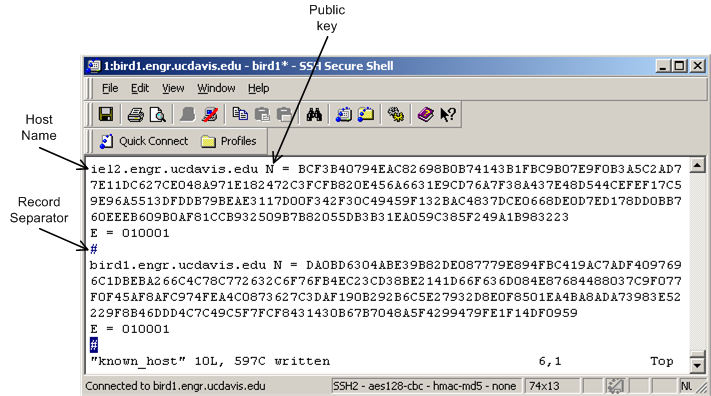
\includegraphics[scale=0.5]{figure/knownhost}
   \caption{A sample known host file.}
   \label{fig:knownhost}
\end{center}
\end{figure*}
% FIGURE }}}
%%%%%%%%%%%%%%%%%%%%%%%%%%%%%%%%%%%%%%%%%%%%%%%%%%%%%%%%%%%%%%%%%%%%%%

%%%%%%%%%%%%%%%%%%%%%%%%%%%%%%%%%%%%%%%%%%%%%%%%%%%%%%%%%%%%%%%%%%%%%%
% Known Host file {{{
\subsection{Known Host File}
After creating the key files for all the agencies in a network the 
  \textit{known\_host} file needs to be created manully.
The sample \textit{known\_host} file is shown in Figure ~\ref{fig:knownhost}. 
To proceed, create a file using a text editor with name 
  \textit{known\_host}. 
Type the name of the first agency (as shown \textit{Host Name} in 
Figure ~\ref{fig:knownhost}) and 
copy its public key from \textit{rsa\_pub} file. Insert the record 
separation character \# and type the same for second agency and continue.
Make sure that the name for the \textit{known\_host} file is 
\textit{``known\_host"}. After creating the 
\textit{known\_host} file, copy the \textit{known\_host} file to each \
agency and the \textit{rsa\_priv} file on the respective
agencies (the same directory from where you will run the Mobile-C 
agency). 
Public and private key files are always created as a pair this means that
  any text encrypted with the public key can only be decrypted with the
  corresponding (paired) private key.
Therefore, please make sure that the copied private key 
(\textit{rsa\_priv}) to an agency must correspond to the public key
that is mentioned infront of the name of this agency in \textit{
known\_host} file.
% }}} Known Host File
%%%%%%%%%%%%%%%%%%%%%%%%%%%%%%%%%%%%%%%%%%%%%%%%%%%%%%%%%%%%%%%%%%%%%%

%}}} Preparation to Run Security Enabled Agency
%%%%%%%%%%%%%%%%%%%%%%%%%%%%%%%%%%%%%%%%%%%%%%%%%%%%%%%%%%%%%%%%%%%%%

%%%%%%%%%%%%%%%%%%%%%%%%%%%%%%%%%%%%%%%%%%%%%%%%%%%%%%%%%%%%%%%%%%%%%
% Examples {{{
\section{Examples -- Mobile-C Security}
A Mobile-C security enable agency can be executed with encypted or plaintext
  private key. 
When you execute a Mobile-C agency it will look for private key file named
  \textit{rsa\_priv} in the current directory. 
If the private key is encrypted and the passphrase is not provided in Mobile-C
  agency C program then it will prompt for the passphrase.
\texttt{<MCPACKAGE>/demos/} contains two demos 
  (\textit{hello\_world\_secure} and \textit{multi\_task\_example\_secure}) that 
  uses private key in plain text.

Please note that for \textit{hello\_world\_secure} demo, the private and public
  key pair is same for client and server, that is both the client and server 
  program run on the same machine (iel2.engr.ucdavis.edu).
To run the demo in your machine, you to write the name of your machine in 
  \textit{known\_host} file and the mobile agent file (\textit{test1.xml}) 

To run client and server agencies on the two different machines, you need to
  create a pair of public and private keys (see section 9.3.1) and that 
  is for the second machine.  
The first agency can use the already created key files that are provided with
  demos.
After creating the key files, edit the \textit{known\_host} file by including
  the name of other machine and newly created public key from file 
  (\textit{rsa\_priv}), for details see section 9.3.2.
Also copy the newly generated private key file (\textit{rsa\_priv}) and 
  updated \textit{known\_host} file on the other machine in the same 
  directory from where Mobile-C agency will be executed.
Now start the server program and then the client program.

Please note that when you build the demos, the executable 
 files ( \textit{client} and  \textit{server}) for demo 
 \textit{hello\_world \_secure} are in 
 directories \textit{hello\_world\_secure/client} and 
 \textit{hello\_world\_ secure/server} respectively. Similarly, the executable 
 files (\textit{client},  \textit{server1} and  \textit{server2} ) for demo
  \textit{multi\_task\_example\_secure} are in directories 
   \textit{multi\_task\_e xample\_secure/client}, 
   \textit{multi\_task\_example\_secure/server1} and
   \textit{multi\_task\_example\_secure/server2} respectively.

Each agency uses a separate \textit{known\_host},
  public(\textit{rsa\_pub}) and private key {\textit{rsa\_priv} pair files. 

\begin{Program}[!t]
\begin{center}
   {\footnotesize \linespread{1.0} \verbatiminput{../demos/mobilec_security/hello_world_secure/server.c }}
\end{center}
\caption{ A sample server side code for security enable agency 
       (\textit{../demos/mobilec\_security/hello\_world\_secure/server.c})}
\label{prog:security_server}
\end{Program}

\begin{Program}[!t]
\begin{center}
   {\footnotesize \linespread{1.0} \verbatiminput{../demos/mobilec_security/hello_world_secure/client.c }}
\end{center}
\caption{ A sample client side code for security enable agency
        (\textit{../demos/mobilec\_security/hello\_world\_secure/client.c})}
\label{prog:security_client}
\end{Program}

The programs \ref{prog:security_server} and \ref{prog:security_client} show 
  \textit{hello\_world\_secure} server and client code respectively.
Please note that the \textit{MC\_AgencyOptions\_t} is required only if the 
  private key file is encrypted. 
Since both programs use the private key file (\textit{rsa\_priv}) in plaintext
  so \textit{MC\_AgencyOptions\_t} is NULL in \textit{MC\_Initialize} function.

If you generate the private key file (\textit{rsa\_priv}) in encrypted form 
   (see section 9.3.1) then the Mobile-C agency requires the same passphrase 
    to decrypt its private key that you have entered to encrypted this file.
In this case \textit{MC\_AgencyOptions\_t} should not be NULL. 
It is a possible that passphrase would not be privided in the code. 
That is, this code can be run if 
  \textit{strcpy(options.passphrase, "xxxx");} is commented out.
In this case, if the private key is encyrpted the Mobile-C agency
  would prompt to enter passphrase at startup otherwise not. 

%To run the these programs in your machine you need to replace 
%  \textit{rabbit.engr.ucdavis.edu} to your machine name in 
%  \textit{client.c}, \textit{test1.xml} and \textit{known\_host}
%  file.
%The \textit{test1.xml} is a hello world mobile agent. \
     

% }}} Example


%%%%%%%%%%%%%%%%%%%%%%%%%%%%%%%%%%%%%%%%%%%%%%%%%%%%%%%%%%%%%%%%%%%%%%

% }}} Mobile-C Security Module
%%%%%%%%%%%%%%%%%%%%%%%%%%%%%%%%%%%%%%%%%%%%%%%%%%%%%%%%%%%%%%%%%%%%%%

%%%%%%%%%%%%%%%%%%%%%%%%%%%%%%%%%%%%%%%%%%%%%%%%%%%%%%%%%%%%%%%%%%%%%%
%{{{Communication With Other FIPA Compliant Agent Systems
\chapter{Communication With Other FIPA Compliant Agent Systems}
This section provides some brief examples regarding communication
between Mobile-C and other FIPA compliant agent systems.
\subsection{Example: Receiving a message from a JADE agent}
The following section contains details regarding an example where a
Mobile-C agent receives a message from a JADE agent. This example is
included to provide a brief overview of how FIPA ACL communication
operates between Mobile-C agencies and JADE agencies.

\subsubsection{Start a Mobile-C Agency}
The first step in the example is to start a Mobile-C agency and a suitable
agent to wait for a message. An example agency which performs these tasks
may be found in the directory \texttt{<MCPACKAGE>/demos/ jade\_to\_mc\_example/}.
To start the agency, simply go to the directory and execute the server
with the command
\begin{verbatim}
./server
\end{verbatim}
The server will start and load the sample agent named ``mobagent1'' in one step,
which should produce the following output (or similar):
\begin{verbatim}
Mobile-C Started

MobileC > This is mobagent1 from the agency at port 5050.
Now, I am going to wait until I receive a message. Waiting...
\end{verbatim}

\subsubsection{Create a JADE container}
The next step is to start a JADE agency. Instructions on how to obtain and
install JADE may be found at the website \texttt{<http://jade.tilab.com>} .
Once JADE in installed, use the command
\begin{verbatim}
java jade.Boot -gui
\end{verbatim}
to start a JADE container. Note that the command may vary across systems depending
on your java distribution and system setup. This command should produce a window
similar to the following:

\begin{center}
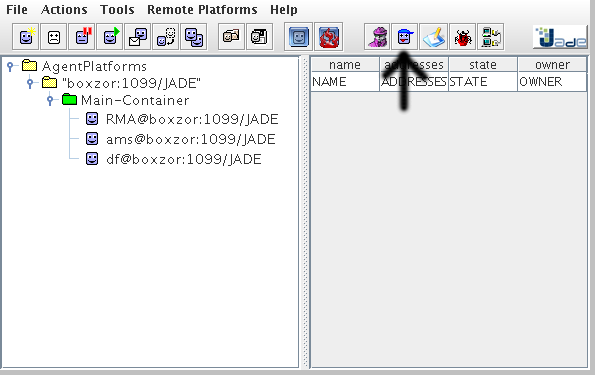
\includegraphics[width=4in]{figure/jade_to_mc_example/jade_main_window.png}
\end{center}

\subsubsection{Start a JADE dummy agent}
The next step is to start a ``dummy'' agent by clicking on the button indicated by the 
large arrow in the previous figure. This should produce a second window
which should resemble the following image.

\begin{center}
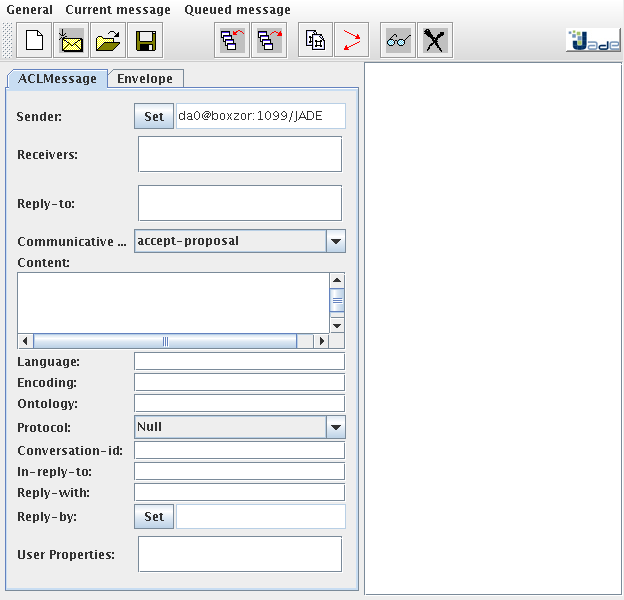
\includegraphics[width=4in]{figure/jade_to_mc_example/dummy_agent_window_blank.png}
\end{center}

\subsubsection{Send a message to Mobile-C}
There are several fields in this empty ACL message that need to be set before the
message will be successfully passed to our Mobile-C agent. The first field to fill
out is the \texttt{Receivers}, which indicates the recipients for our message.
We wish for our Mobile-C agent ``mobagent1'' to be our sole recipient. Add 
``mobagent1'' by right-clicking on the \texttt{Receivers} textbox and selecting the
\texttt{Add} option. Fill out the box as shown in the following image:

\begin{center}
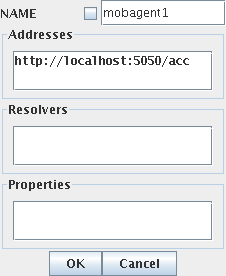
\includegraphics[width=2in]{figure/jade_to_mc_example/dummy_agent_receiver_window.png}
\end{center}

After setting the receiver, the rest of the message may be set to whatever is desired.
For this example, our sample message may be seen on the following image.

\begin{center}
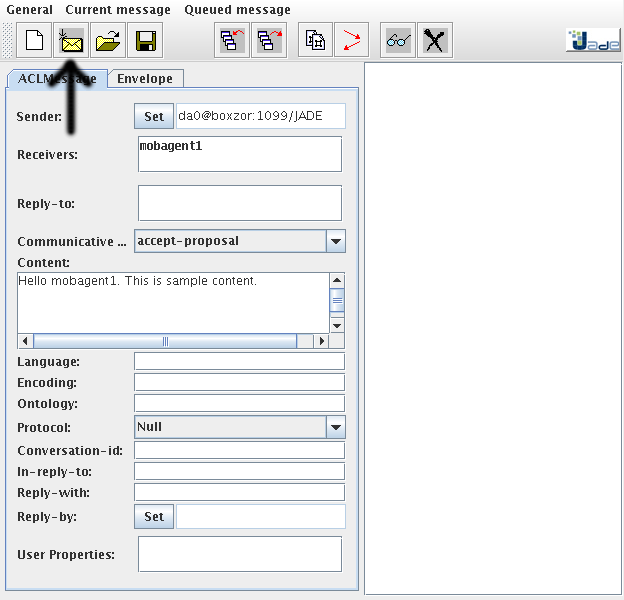
\includegraphics[width=4in]{figure/jade_to_mc_example/dummy_agent_window_complete.png}
\end{center}

Once your desired message parameters are in place, click on the ``Send Message'' button
indicated by the arrow in the previous figure. The message will be sent to the agent
waiting at the Mobile-C agency that was previously started. The agent should
receive the message and produce the following output:
\begin{verbatim}
mobagent1 Got a message!
Message is from da0@boxzor:1099/JADE
The content is Hello mobagent1. This is sample content.
\end{verbatim}
This indicates that \texttt{mobagent1} has successfully received the
message from JADE.

\subsection{Example: Sending a message from Mobile-C to JADE}
This example illustrates a Mobile-C agent sending an ACL message to a
JADE agent.  The example will be presented in a step by step fashion and all
files may be found in the directory \texttt{<MCPACKAGE>/demos/mc\_to\_jade\_example/}.

\subsubsection{Start a JADE container with a ``PingAgent'' agent}
The first step is to start a JADE container with a responsive agent. In this
example, we will use a demo ``PingAgent'' agent which is provided with JADE. The
agent source code may be found in the JADE subdirectory 
\texttt{jade/src/examples/PingAgent/PingAgent.java} . After installing JADE,
run the command
\begin{verbatim}
java jade.Boot pingme:examples.PingAgent.PingAgent
\end{verbatim}
from the \texttt{jade/src/} directory to start a JADE main container and 
invoke an agent of type ``PingAgent'' named ``pingme''. The ``PingAgent'' agent
contains a behaviour which receives messages and replies with a standard 
reply message. The ``PingAgent'' expects incoming messages to have a performative
of ``query-ref'', and for the content field to contain the text ``ping''. 

\subsubsection{Start a Mobile-C agency with a sender agent}
A Mobile-C agency and agent for use in the example has already been
created and reside in the directory \texttt{<MCPACKAGE>/demos/mc\_to\_jade\_example/} .
After compiling Mobile-C and the Mobile-C demos, simply go to the directory and
run the 'client' executable.
\begin{verbatim}
./client
\end{verbatim}
The executable will automatically start a Mobile-C agency and load an agent
named ``mobagent1''. The agent is programmed to send an ACL message to 
``pingme'' at the local JADE container and wait for a response message. 
Upon receiving the response, the agent will print the contents of the 
response message. The Mobile-C agent output should look something like
\begin{verbatim}
Mobile-C Started
Sending agent to self...
Done.
mobagent2 Creating new ACL message...
mobagent2 sending ACL message...
Received a message from pingme@boxzor:1099/JADE.
Content is 'alive'.
\end{verbatim}
%}}}
%%%%%%%%%%%%%%%%%%%%%%%%%%%%%%%%%%%%%%%%%%%%%%%%%%%%%%%%%%%%%%%%%%%%%%

%%%%%%%%%%%%%%%%%%%%%%%%%%%%%%%%%%%%%%%%%%%%%%%%%%%%%%%%%%%%%%%%%%%%%%
% Bibliography {{{
%\phantomsection
%\addcontentsline{toc}{chapter}{Bibliography}
\bibliographystyle{IEEEtran}
%\bibliography{/home/chgroup/project/paper/ielpaper}
\bibliography{ielpaper}
\pagebreak
% }}} Bibliography 
%%%%%%%%%%%%%%%%%%%%%%%%%%%%%%%%%%%%%%%%%%%%%%%%%%%%%%%%%%%%%%%%%%%%%%

%%%%%%%%%%%%%%%%%%%%%%%%%%%%%%%%%%%%%%%%%%%%%%%%%%%%%%%%%%%%%%%%%%%%%%
% Appendix {{{
\appendix
\chapter{Mobile-C API in the C/C++ Binary Space \label {appendix}}
\lhead{Mobile-C API in the C/C++ Binary Space}
\noindent
The header file {\bf libmc.h} defines all the data types, macros 
and function prototypes for the Mobile-C library.
The header file is used in the C/C++ binary space.

\begin{table}[!h]
\capstart
\begin{center}
\caption{Data types defined in {\bf libmc.h}.}
\begin{tabular}{p{50 mm}p{110 mm}}
\hline
Data Type & Description \\
\hline
{\bf MCAgency\_t} & A handle containing information of an agency. \\
{\bf MCAgent\_t} & A handle containing information of a mobile agent. \\
{\bf MCAgencyOptions\_t} & A structure containing information about which thread(s) to be activated and the default agent status specified by a user. \\
\hline
\end{tabular}
\end{center}
\label{mobilec_datatype}
\end{table}

The header file {\bf fipa\_acl.h} contains datatype and macros related to 
FIPA ACL messaging, as described in Chapter \ref{chap:fipa}. This header
file may be used in both C/C++ binary space, as well as agent space.

\begin{table}[!h]
\capstart
\begin{center}
\caption{Data types defined in {\bf fipa\_acl.h}.}
\begin{tabular}{p{50 mm}p{110 mm}}
\hline
Data Type & Description \\
\hline
{\bf fipa\_acl\_message\_t} & A structure containing a FIPA ACL message. \\
\hline
\end{tabular}
\end{center}
\label{fipa_datatype}
\end{table}

\pagebreak

\begin{table}[!h]
\capstart
\begin{center}
\caption{Macros defined in {\bf libmc.h}.}
\begin{tabular}{p{50 mm}p{110 mm}}
\hline
Macro & Description \\
\hline
{\texttt enum MC\_ThreadIndex\_e} & \\
\hline
{\bf MC\_THREAD\_AI} \index{MC\_THREAD\_AI} & Identifier for agent initalizing thread. \\
{\bf MC\_THREAD\_AM} \index{MC\_THREAD\_AM} & Identifier for agent managing thread. \\
{\bf MC\_THREAD\_CL} \index{MC\_THREAD\_CL} & Identifier for connection listening thread. \\
{\bf MC\_THREAD\_MR} \index{MC\_THREAD\_MR} & Identifier for message receiving thread. \\
{\bf MC\_THREAD\_MS} \index{MC\_THREAD\_MS} & Identifier for message sending thread. \\
{\bf MC\_THREAD\_CP} \index{MC\_THREAD\_CP} & Identifier for command prompt thread. \\
{\bf MC\_THREAD\_ALL} \index{MC\_THREAD\_ALL} & Identifier for all threads. \\
\hline
{\texttt enum MC\_Signal\_e} & \\
\hline
{\bf MC\_RECV\_CONNECTION} \index{MC\_RECV\_CONNECTION} & Signal activated after an agency accepts a connection. \\
{\bf MC\_RECV\_MESSAGE} \index{MC\_RECV\_MESSAGE} & Signal activated after an agency receives an ACL message. \\
{\bf MC\_RECV\_AGENT} \index{MC\_RECV\_AGENT} & Signal activated after an agency receives a mobile agent. \\
{\bf MC\_RECV\_RETURN} \index{MC\_RECV\_RETURN} & Signal activated after an agency receives return data from a completed mobile agent. \\
{\bf MC\_EXEC\_AGENT} \index{MC\_EXEC\_AGENT} & Signal activated after a mobile agent is executed. \\
{\bf MC\_ALL\_SIGNALS} \index{MC\_ALL\_SIGNALS} & Signal activated after any of the above four events occurs. \\
\hline
{\texttt enum MC\_AgentType\_e} \index{MC\_AgentType\_e}& \\
\hline
{\bf MC\_REMOTE\_AGENT} \index{MC\_REMOTE\_AGENT} & Identifier for a remote mobile agent. \\
{\bf MC\_LOCAL\_AGENT} \index{MC\_LOCAL\_AGENT} & Identifier for a local mobile agent.\\
{\bf MC\_RETURN\_AGENT} \index{MC\_RETURN\_AGENT} & Identifier for a return mobile agent. \\
\hline
{\texttt enum MC\_AgentStatus\_e} \index{MC\_AgentStatus\_e} & \\
\hline
{\bf MC\_WAIT\_CH} \index{MC\_WAIT\_CH} & Value indicating a mobile agent is waiting to be executed. \\
{\bf MC\_WAIT\_MESSGSEND} \index{MC\_WAIT\_MESSGSEND}& Value indicating a mobile agent is waiting to be exported to another agency. \\
{\bf MC\_AGENT\_ACTIVE} \index{MC\_AGENT\_ACTIVE}& Value indicating a mobile agent is being executed. \\
{\bf MC\_AGENT\_NEUTRAL} \index{MC\_AGENT\_NEUTRAL}& Value indicating a mobile agent is waiting for an unspecified reason. \\
{\bf MC\_AGENT\_SUSPENDED} \index{MC\_AGENT\_SUSPENDED}& Value indicating a mobile agent is being suspended. \\
{\bf MC\_WAIT\_FINISHED} \index{MC\_WAIT\_FINISHED}& Value indicating a mobile agent has been executed and is waiting to be removed. \\
\hline
\end{tabular}
\end{center}
\label{mobilec_macro}
\end{table}

\begin{table}[!hp]
\capstart
\begin{center}
\caption{Macros defined in {\bf fipa\_acl.h}. Detailed documentation for the
FIPA performatives and protocols may be found in the FIPA specifications at
\texttt{http://www.fipa.org}.}
\begin{tabular}{p{90 mm}p{70 mm}}
\hline
Macro & Description \\
\hline
{\texttt fipa\_performative\_e \index{fipa\_performative\_e}} & \\
\hline
{\bf FIPA\_ACCEPT\_PROPOSAL} \index{FIPA\_ACCEPT\_PROPOSAL} & The \texttt{accept-proposal} performative. \\
{\bf FIPA\_AGREE} \index{FIPA\_AGREE} & The \texttt{agree} performative. \\
{\bf FIPA\_CANCEL} \index{FIPA\_CANCEL} & The \texttt{cancel} performative. \\
{\bf FIPA\_CALL\_FOR\_PROPOSAL} \index{FIPA\_CALL\_FOR\_PROPOSAL} & The \texttt{call-for-proposal} performative. \\
{\bf FIPA\_CONFIRM} \index{FIPA\_CONFIRM} & The \texttt{confirm} performative. \\
{\bf FIPA\_DISCONFIRM} \index{FIPA\_DISCONFIRM} & The \texttt{disconfirm} performative. \\
{\bf FIPA\_FAILURE} \index{FIPA\_FAILURE} & The \texttt{failure} performative. \\
{\bf FIPA\_INFORM} \index{FIPA\_INFORM} & The \texttt{inform} performative. \\
{\bf FIPA\_INFORM\_IF} \index{FIPA\_INFORM\_IF} & The \texttt{inform-if} performative. \\
{\bf FIPA\_INFORM\_REF} \index{FIPA\_INFORM\_REF} & The \texttt{inform-ref} performative. \\
{\bf FIPA\_NOT\_UNDERSTOOD} \index{FIPA\_NOT\_UNDERSTOOD} & The \texttt{not-understood} performative. \\
{\bf FIPA\_PROPOGATE} \index{FIPA\_PROPOGATE} & The \texttt{propogate} performative. \\
{\bf FIPA\_PROPOSE} \index{FIPA\_PROPOSE} & The \texttt{propose} performative. \\
{\bf FIPA\_PROXY} \index{FIPA\_PROXY} & The \texttt{proxy} performative. \\
{\bf FIPA\_QUERY\_IF} \index{FIPA\_QUERY\_IF} & The \texttt{query-if} performative. \\
{\bf FIPA\_QUERY\_REF} \index{FIPA\_QUERY\_REF} & The \texttt{query-ref} performative. \\
{\bf FIPA\_REFUSE} \index{FIPA\_REFUSE} & The \texttt{refuse} performative. \\
{\bf FIPA\_REJECT\_PROPOSAL} \index{FIPA\_REJECT\_PROPOSAL} & The \texttt{reject-proposal} performative. \\
{\bf FIPA\_REQUEST} \index{FIPA\_REQUEST} & The \texttt{request} performative. \\
{\bf FIPA\_REQUEST\_WHEN} \index{FIPA\_REQUEST\_WHEN} & The \texttt{request-when} performative. \\
{\bf FIPA\_REQUEST\_WHENEVER} \index{FIPA\_REQUEST\_WHENEVER} & The \texttt{request-whenever} performative. \\
{\bf FIPA\_SUBSCRIBE} \index{FIPA\_SUBSCRIBE} & The \texttt{subscribe} performative. \\
\hline
{\texttt enum fipa\_protocol\_e} & \\
\hline
{\bf FIPA\_PROTOCOL\_REQUEST} \index{FIPA\_PROTOCOL\_REQUEST} & The FIPA \texttt{request} protocol. \\
{\bf FIPA\_PROTOCOL\_QUERY} \index{FIPA\_PROTOCOL\_QUERY} & The FIPA \texttt{query} protocol. \\
{\bf FIPA\_PROTOCOL\_REQUEST\_WHEN} \index{FIPA\_PROTOCOL\_REQUEST\_WHEN} & The FIPA \texttt{request-when} protocol. \\
{\bf FIPA\_PROTOCOL\_CONTRACT\_NET} \index{FIPA\_PROTOCOL\_CONTRACT\_NET} & The FIPA \texttt{contract-net} protocol. \\
{\bf FIPA\_PROTOCOL\_ITERATED\_CONTRACT\_NET} \index{FIPA\_PROTOCOL\_ITERATED\_CONTRACT\_NET} & The FIPA \texttt{iterated-contract-net} protocol. \\
{\bf FIPA\_PROTOCOL\_ENGLISH\_AUCTION} \index{FIPA\_PROTOCOL\_ENGLISH\_AUCTION} & The FIPA \texttt{english-auction} protocol. \\
{\bf FIPA\_PROTOCOL\_DUTCH\_AUCTION} \index{FIPA\_PROTOCOL\_DUTCH\_AUCTION} & The FIPA \texttt{dutch-auction} protocol. \\
{\bf FIPA\_PROTOCOL\_BROKERING} \index{FIPA\_PROTOCOL\_BROKERING} & The FIPA \texttt{brokering} protocol. \\
{\bf FIPA\_PROTOCOL\_RECRUITING} \index{FIPA\_PROTOCOL\_RECRUITING} & The FIPA \texttt{recruiting} protocol. \\
{\bf FIPA\_PROTOCOL\_SUBSCRIBE} \index{FIPA\_PROTOCOL\_SUBSCRIBE} & The FIPA \texttt{subscribe} protocol. \\
{\bf FIPA\_PROTOCOL\_PROPOSE} \index{FIPA\_PROTOCOL\_PROPOSE} & The FIPA \texttt{propose} protocol. \\
{\bf FIPA\_PROTOCOL\_END} \index{FIPA\_PROTOCOL\_END} & The FIPA \texttt{end} protocol. \\
\hline
\end{tabular}
\end{center}
\label{fipa_macro}
\end{table}

\begin{table}[!hp]
\capstart
\begin{center}
\caption{Functions in the C/C++ binary space.}
\begin{tabular}{p{78 mm}p{77 mm}}
%\begin{tabular}{ll}
\hline
Function & Description \\
\hline
{\bf MC\_AclAddReceiver()} \dotfill & Add a receiver to an ACL message. \\
{\bf MC\_AclAddReplyTo()} \dotfill & Add a reply-to address to an ACL message. \\
{\bf MC\_AclGetContent()} \dotfill & Get the content of an ACL message. \\
{\bf MC\_AclGetConversationID()} \dotfill & Get the conversation id from an ACL message. \\
{\bf MC\_AclGetPerformative()} \dotfill & Get the performative of an ACL message. \\
{\bf MC\_AclGetProtocol()} \dotfill & Get the protocol from an ACL message. \\
{\bf MC\_AclGetSender()} \dotfill & Get the sender of an ACL message. \\
{\bf MC\_AclNew()} \dotfill & Allocate a new FIPA ACL message. \\
{\bf MC\_AclPost()} \dotfill & Post a FIPA ACL message to an agent's mailbox. \\
{\bf MC\_AclReply()} \dotfill & Allocate a new FIPA ACL message automatically addressed to the sender of a previous message. \\
{\bf MC\_AclRetrieve()} \dotfill & Retrieve an ACL message from an agent's mailbox. \\
{\bf MC\_AclSetContent()} \dotfill & Set the content of an ACL message. \\
{\bf MC\_AclSetConversationID()} \dotfill & Set the conversation id of an ACL message. \\
{\bf MC\_AclSetPerformative()} \dotfill & Set the performative of an ACL message. \\
{\bf MC\_AclSetProtocol()} \dotfill & Set the protocol of an ACL message. \\
{\bf MC\_AclSetSender()} \dotfill & Set the sender of an ACL message. \\
{\bf MC\_AclWaitRetrieve()} \dotfill & Wait for a message to arrive at an agent's mailbox. \\
{\bf MC\_AgentAddTask()} \dotfill & Add a task to an agent based off of C source code. \\
{\bf MC\_AgentAddTaskFromFile()} \dotfill & Add a task to an agent based off of a C source code file. \\
{\bf MC\_AgentAttachFile()} \dotfill & Attach a file to the agent's current task. \\
{\bf MC\_AgentListFiles()} \dotfill & List files attached to an agent's task. \\
{\bf MC\_AgentRetrieveFile()} \dotfill & Retrieve and save an agent's attached file onto the filesystem. \\
{\bf MC\_AgentReturnArrayDim()} \dotfill & Get the dimension of an array returned by an agent. \\
{\bf MC\_AgentReturnArrayExtent()} \dotfill & Get the extent of a dimension of an array returned by an agent. \\
{\bf MC\_AgentReturnArrayNum()} \dotfill & Get the number of elements of an array returned by an agent. \\
{\bf MC\_AgentReturnDataGetSymbolAddr()} \dotfill & Get a pointer to an array returned by an agent. \\
{\bf MC\_AgentReturnDataSize()} \dotfill & Get the size of a single element of the array. \\
{\bf MC\_AgentReturnDataType()} \dotfill & Get the type of the array. \\
{\bf MC\_AgentReturnIsArray()} \dotfill & Determine if the returned variable is an array. \\
{\bf MC\_AddAgent()} \dotfill & Add a mobile agent into an agency. \\
{\bf MC\_AddAgentInitCallback()} \dotfill & Add an agent initialization callback function into an agency. \\
{\bf MC\_AddStationaryAgent()} \dotfill & Add a mobile agent into an agency. \\
%{\bf MC\_AgentVariableRetrieve()} & Retrieve a saved variable from an agent's prior task. \\
%{\bf MC\_AgentVariableSave()} & Save an agent's task variable for migration. \\
{\bf MC\_Barrier()} \dotfill & Block until all agents in an agency have called this function. \\
{\bf MC\_BarrierDelete()} \dotfill & Delete a Mobile-C barrier. \\
{\bf MC\_BarrierInit()} \dotfill & Initialize a Mobile-C barrier. \\
{\bf MC\_CallAgentFunc()} \dotfill & Call a function defined in an agent. \\
{\bf MC\_CallAgentFuncV()} \dotfill & Call a function defined in an agent. \\
\hline
\end{tabular}
\end{center}
\label{mobilec_api_cbinary}
\end{table}

\addtocounter{table}{-1}
\begin{table}[!hp]
\capstart
\begin{center}
\caption{Functions in the C/C++ binary space (contd.).}
%\begin{tabular}{ll}
\begin{tabular}{p{78 mm}p{77 mm}}
\hline
Function & Description \\
\hline
{\bf MC\_CallAgentFuncVar()} \dotfill & Call a function defined in an agent. \\
{\bf MC\_ChInitializeOptions()} \dotfill & Set the initialization options for a Ch to be used as one AEE in an agency. \\
{\bf MC\_ComposeAgent()} \dotfill & Compose an agent from program source code. \\
{\bf MC\_ComposeAgentS()} \dotfill & [Deprecated] Compose an agent from program source code with a workgroup code. \\
{\bf MC\_ComposeAgentWithWorkgroup()} \dotfill & Compose an agent from program source code with a workgroup code. \\
{\bf MC\_ComposeAgentFromFile()} \dotfill & Compose an agent from a program source code file. \\
{\bf MC\_ComposeAgentFromFileS()} \dotfill & [Deprecated] Compose an agent from a program source code file with a workgroup code. \\
{\bf MC\_ComposeAgentFromFileWithWorkgroup()} & Compose an agent from a program source code file with a workgroup code. \\
{\bf MC\_CondBroadcast()} \dotfill & Wake up all agents/threads waiting on a condition variable. \\
{\bf MC\_CondReset()} \dotfill & Reset a Mobile-C condition variable. \\
{\bf MC\_CondSignal()} \dotfill & Signal another agent that is waiting on a condition variable. \\
{\bf MC\_CondWait()} \dotfill & Cause the calling agent or thread to wait on a Mobile-C condition variable with the ID specified by the argument. \\
{\bf MC\_CopyAgent()} \dotfill & Perform a deep copy to copy an agent. \\
{\bf MC\_DeleteAgent()} \dotfill & Stop and remove an agent from an agency. \\
{\bf MC\_DeregisterService()} \dotfill & Deregister a service with the Directory Facilitator. \\
{\bf MC\_End()} \dotfill & Terminate a Mobile-C agency. \\
{\bf MC\_FindAgentByID()} \dotfill & Find a mobile agent by its ID number in an agency.\\
{\bf MC\_FindAgentByName()} \dotfill & Find a mobile agent by its name in an agency. \\
{\bf MC\_GetAgentArrivalTime()} \dotfill & Get the time when an agent arrives an agency. \\
{\bf MC\_GetAgentExecEngine()} \dotfill & Get the AEE associated with a mobile agent in an agency. \\
{\bf MC\_GetAgentID()} \dotfill & Get the ID of an agent. \\
{\bf MC\_GetAgentName()} \dotfill & Get the name of an agent. \\
{\bf MC\_GetAgentNumTasks()} \dotfill & Get the number of tasks a mobile agent has. \\
{\bf MC\_GetAgentReturnData()} \dotfill & [Deprecated] Get the return data of a mobile agent. \\
{\bf MC\_GetAgentStatus()} \dotfill & Get the status of a mobile agent in an agency. \\
{\bf MC\_GetAgentType()} \dotfill & Get the type of a mobile agent. \\
{\bf MC\_GetAgentXMLString()} \dotfill & Retrieve a mobile agent message in XML format as a character string. \\
{\bf MC\_GetAllAgents()} \dotfill & Obtain all the agents in an agency. \\
{\bf MC\_HaltAgency()} \dotfill & Halt an agency's operation. \\
{\bf MC\_Initialize()} \dotfill & Start a Mobile-C agency and return a handle of the launched agency. \\
{\bf MC\_InitializeAgencyOptions()} \dotfill & Initialize Mobile-C options. \\
{\bf MC\_LoadAgentFromFile()} \dotfill & Load an agent from an XML file into a local agency.\\
\hline
\end{tabular}
\end{center}
\end{table}
\pagebreak

\addtocounter{table}{-1}
\begin{table}[!hp]
\capstart
\begin{center}
\caption{Functions in the C/C++ binary space (contd.).}
%\begin{tabular}{ll}
\begin{tabular}{p{63 mm}p{97 mm}}
\hline
Function & Description \\
\hline
{\bf MC\_MainLoop()} \dotfill & Cause the calling thread to wait indefinitely on an agency.\\
{\bf MC\_MigrateAgent()} \dotfill & Migrate an agent. \\
{\bf MC\_MutexLock()} \dotfill & Lock a previously initialized Mobile-C synchronization variable as a mutex. \\
{\bf MC\_MutexUnlock()} \dotfill & Unlock a locked Mobile-C synchronization variable. \\
{\bf MC\_PrintAgentCode()} \dotfill & Print a mobile agent code for inspection. \\
{\bf MC\_RegisterService()} \dotfill &  Register a new service with the Directory Facilitator. \\
{\bf MC\_ResetSignal()} \dotfill &  Reset the Mobile-C signalling system. \\
{\bf MC\_ResumeAgency()} \dotfill &  Resume an agency's operation. \\
{\bf MC\_RetrieveAgent()} \dotfill & Retrieve the first neutral mobile agent from a mobile agent list. \\
{\bf MC\_RetrieveAgentCode()} \dotfill & Retrieve a mobile agent code in the form of a character string. \\
{\bf MC\_SearchForService()} \dotfill & Search the Directory Facilitator for a service. \\
{\bf MC\_SemaphorePost()} \dotfill & Unlock one resource from a Mobile-C semaphore. \\
{\bf MC\_SemaphoreWait()} \dotfill & Allocate one resource from a Mobile-C synchronization semaphore variable. \\
{\bf MC\_SendAgent()} \dotfill & Send an ACL mobile agent message to a remote agency. \\
{\bf MC\_SendAgentFile()} \dotfill & Send an ACL mobile agent message saved as a file to a remote agency. \\
{\bf MC\_SendAgentMigrationMessage()} \dotfill & [Deprecated] Send an ACL mobile agent message to a remote agency. \\
{\bf MC\_SendAgentMigrationMessageFile()} \dotfill & [Deprecated] Send an ACL mobile agent message saved as a file to a remote agency. \\
{\bf MC\_SendSteerCommand()} \dotfill & Send a command to control a steerable binary space function. \\
{\bf MC\_SetAgentStatus()} \dotfill & Set the status of a mobile agent in an agency. \\
{\bf MC\_SetDefaultAgentStatus()} \dotfill & Assign a user defined default status to all incoming mobile agents. \\
{\bf MC\_SetThreadOff()} \dotfill & Deactivate a thread in an agency. \\
{\bf MC\_SetThreadOn()} \dotfill & Activate a thread in an agency. \\
{\bf MC\_Steer()} \dotfill & Set up a steerable binary space function. \\
{\bf MC\_SteerControl()} \dotfill & Retrieve a steering command from the mobile agent space. \\
{\bf MC\_SyncDelete()} \dotfill & Delete a previously initialized synchronization variable. \\
{\bf MC\_SyncInit()} \dotfill & Initialize a new synchronization variable. \\
{\bf MC\_TerminateAgent()} \dotfill & Terminate the execution of a mobile agent in an agency. \\
%{\bf MC\_Wait()} \dotfill & Cause the calling thread to wait indefinitely on an agency.\\
{\bf MC\_WaitAgent()} \dotfill & Cause the calling thread to wait until a mobile agent is received. \\
{\bf MC\_WaitRetrieveAgent()} \dotfill & Block the calling thread until a mobile agent arrives, and return the mobile agent instead of executing it. \\
{\bf MC\_WaitSignal()} \dotfill & Block until one of the signals in the second argument is signalled.\\
\hline
\end{tabular}
\end{center}
\end{table}
\pagebreak

\newpage
\rhead{\bf MC\_AclGetProtocol()}
\noindent
\vspace{5pt}
\rule{6.5in}{0.015in}
\noindent
\phantomsection
{\LARGE \bf MC\_AclGetProtocol()\index{MC\_AclGetProtocol()}}\\
\addcontentsline{toc}{section}{MC\_AclGetProtocol()}
\label{api:MC_Acl_SetProtocol()}

\noindent
{\bf Synopsis}\\
{\bf \#include $<$libmc.h$>$}\\
{\bf enum fipa\_protocol\_e MC\_AclGetProtocol}({\bf fipa\_acl\_message\_t*} acl);\\

\noindent
{\bf Purpose}\\
Get the protocol of an ACL message.\\

\noindent
{\bf Return Value}\\
Retuns a valid FIPA Protocol enumeration on success or -1 on failure.\\

\noindent
{\bf Parameters}
\vspace{-0.1in}
\begin{description}
\item
\begin{tabular}{p{10 mm}p{145 mm}} 
$acl$ & An initialized ACL message. 
\end{tabular}
\end{description}

\noindent
{\bf Description}\\
This function is used to get the FIPA ACL protocol from an ACL message. 
The protocol may be any valid FIPA protocol listed in the table 
below. The protocol field is not required to be set for a valid ACL
message. \\
\begin{tabular}{ll}
Enumerated Value & FIPA Protocol \\ \hline
\texttt{FIPA\_PROTOCOL\_REQUEST} & FIPA \texttt{request} protocol. \\
\texttt{FIPA\_PROTOCOL\_QUERY} & FIPA \texttt{query} protocol. \\
\texttt{FIPA\_PROTOCOL\_REQUEST\_WHEN} & FIPA \texttt{request-when} protocol. \\
\texttt{FIPA\_PROTOCOL\_CONTRACT\_NET} & FIPA \texttt{contract-net} protocol. \\
\texttt{FIPA\_PROTOCOL\_ITERATED\_CONTRACT\_NET} & FIPA \texttt{iterated-contract-net} protocol. \\
\texttt{FIPA\_PROTOCOL\_ENGLISH\_AUCTION} & FIPA \texttt{english-auction} protocol.\\
\texttt{FIPA\_PROTOCOL\_DUTCH\_AUCTION} & FIPA \texttt{dutch-auction} protocol. \\
\texttt{FIPA\_PROTOCOL\_BROKERING} & FIPA \texttt{brokering} protocol. \\
\texttt{FIPA\_PROTOCOL\_RECRUITING} & FIPA \texttt{recruiting} protocol. \\
\texttt{FIPA\_PROTOCOL\_SUBSCRIBE} & FIPA \texttt{subscribe} protocol. \\
\texttt{FIPA\_PROTOCOL\_PROPOSE} & FIPA \texttt{propose} protocol. \\
\end{tabular} \\
Please refer to the FIPA protocol specifications at \texttt{http://www.fipa.org} for 
more details about each of these protocols.


\noindent
{\bf See Also}\\
\texttt{
  MC\_AclSetSender(), MC\_AclAddReceiver(), MC\_AclAddReplyTo(), \linebreak 
    MC\_AclSetContent()
}

%\CPlot::\DataThreeD(), \CPlot::\DataFile(), \CPlot::\Plotting(), \plotxy().\\

\pagebreak
\rhead{\bf MC\_AclAddReceiver()}
\noindent
\vspace{5pt}
\rule{6.5in}{0.015in}
\noindent
\phantomsection
{\LARGE \bf MC\_AclAddReceiver()\index{MC\_AclAddReceiver()}}\\
\addcontentsline{toc}{section}{MC\_AclAddReceiver()}
\label{api:MC_Acl_AddReceiver()}

\noindent
{\bf Synopsis}\\
{\bf \#include $<$libmc.h$>$}\\
{\bf int MC\_AclAddReceiver}({\bf fipa\_acl\_message\_t*} acl, {\bf const char*} name, {\bf const char*} address );\\

\noindent
{\bf Purpose}\\
Add a receiver to the ACL message.\\

\noindent
{\bf Return Value}\\
Returns 0 on success or non-zero on failure.

\noindent
{\bf Parameters}
\vspace{-0.1in}
\begin{description}
\item
\begin{tabular}{p{10 mm}p{145 mm}} 
$acl$ & An initialized ACL message. \\
$name$ & Sets the name of the receiver. \\
$address$ & Sets the address of the receiver. 
\end{tabular}
\end{description}

\noindent
{\bf Description}\\
This function is used to add a receiver to an ACL message. This function 
may be called multiple times on an ACL message. each time this function is 
called, a new receiver is appended to the list of intended receivers
for the ACL message. \\

\noindent
{\bf Example}\\
\noindent
{\footnotesize\verbatiminput{../demos/FIPA_compliant_ACL_messages/fipa_test/test2.xml}}

\noindent
{\bf See Also}\\
\texttt{
  MC\_AclSetPerformative(), MC\_AclSetSender(), MC\_AclAddReplyTo(), 
\linebreak MC\_AclSetContent()}


%\CPlot::\DataThreeD(), \CPlot::\DataFile(), \CPlot::\Plotting(), \plotxy().\\

\pagebreak
\rhead{\bf MC\_AclAddReplyTo()}
\noindent
\vspace{5pt}
\rule{6.5in}{0.015in}
\noindent
\phantomsection
{\LARGE \bf MC\_AclAddReplyTo()\index{MC\_AclAddReplyTo()}}\\
\addcontentsline{toc}{section}{MC\_AclAddReplyTo()}
\label{api:MC_Acl_AddReplyTo()}

\noindent
{\bf Synopsis}\\
{\bf \#include $<$libmc.h$>$}\\
{\bf int MC\_AclAddReplyTo}({\bf fipa\_acl\_message\_t*} acl, {\bf const char*} name, {\bf const char*} address );\\

\noindent
{\bf Purpose}\\
Add a reply-to address to the ACL message.\\

\noindent
{\bf Return Value}\\
Returns 0 on success or non-zero on failure. \\

\noindent
{\bf Parameters}
\vspace{-0.1in}
\begin{description}
\item
\begin{tabular}{p{10 mm}p{145 mm}} 
$acl$ & An initialized ACL message. \\
$name$ & Sets the name of the reply-to destination. \\
$address$ & Sets the address of the reply-to destination. 
\end{tabular}
\end{description}

\noindent
{\bf Description}\\
This function is used to add a reply-to address to an ACL message. This function 
may be called multiple times on an ACL message. each time this function is 
called, a new reply-to address is appended to the list of intended reply-to
addresses for the ACL message. \\

\noindent
{\bf Example}\\
\noindent
{\footnotesize\verbatiminput{../demos/FIPA_compliant_ACL_messages/fipa_test/test2.xml}}

\noindent
{\bf See Also}\\
\texttt{
  MC\_AclSetPerformative(), MC\_AclSetSender(), MC\_AclAddReceiver(), \linebreak
    MC\_AclSetContent()
}

%\CPlot::\DataThreeD(), \CPlot::\DataFile(), \CPlot::\Plotting(), \plotxy().\\

\pagebreak
\rhead{\bf MC\_AclGetContent()}
\noindent
\vspace{5pt}
\rule{6.5in}{0.015in}
\noindent
\phantomsection
{\LARGE \bf MC\_AclGetContent()\index{MC\_AclGetContent()}}\\
\addcontentsline{toc}{section}{MC\_AclGetContent()}
\label{api:MC_Acl_GetContent()}

\noindent
{\bf Synopsis}\\
{\bf \#include $<$libmc.h$>$}\\
{\bf const char* MC\_AclGetContent}({\bf fipa\_acl\_message\_t*} acl);\\

\noindent
{\bf Purpose}\\
Get the content of an ACL message.\\

\noindent
{\bf Return Value}\\
Returns a valid character string or NULL on failure. \\

\noindent
{\bf Parameters}
\vspace{-0.1in}
\begin{description}
\item
\begin{tabular}{p{10 mm}p{145 mm}} 
$acl$ & An initialized ACL message. \\
\end{tabular}
\end{description}

\noindent
{\bf Description}\\
This function gets the ``content'' field of an ACL message. \\

\noindent
{\bf Example}\\
\noindent
{\footnotesize\verbatiminput{../demos/FIPA_compliant_ACL_messages/fipa_test/test2.xml}}

\noindent
{\bf See Also}\\
\texttt{
  MC\_AclSetPerformative(), MC\_AclSetSender(), MC\_AclAddReceiver(), 
    \linebreak MC\_AclAddReplyTo()
}

%\CPlot::\DataThreeD(), \CPlot::\DataFile(), \CPlot::\Plotting(), \plotxy().\\

\pagebreak
\rhead{\bf MC\_AclGetConversationID()}
\noindent
\vspace{5pt}
\rule{6.5in}{0.015in}
\noindent
\phantomsection
{\LARGE \bf MC\_AclGetConversationID()\index{MC\_AclGetConversationID()}}\\
\addcontentsline{toc}{section}{MC\_AclGetConversationID()}
\label{api:MC_Acl_GetConversationID()}

\noindent
{\bf Synopsis}\\
{\bf \#include $<$libmc.h$>$}\\
{\bf const char* MC\_AclGetConversationID}({\bf fipa\_acl\_message\_t*} acl);\\

\noindent
{\bf Purpose}\\
Get the conversation id of an ACL message.\\

\noindent
{\bf Return Value}\\
Returns a character string on success of NULL on failure.\\

\noindent
{\bf Parameters}
\vspace{-0.1in}
\begin{description}
\item
\begin{tabular}{p{10 mm}p{145 mm}} 
$acl$ & An initialized ACL message. 
\end{tabular}
\end{description}

\noindent
{\bf Description}\\
This function gets the ``conversation-id'' field from an ACL message. 
The conversation ID is used to differentiate multiple agent conversations which
may be happening simultaneously between two agents. For more details, please
consult the FIPA specifications at \texttt{http://www.fipa.org}.\\

\noindent
{\bf See Also}\\
\texttt{
  MC\_AclSetPerformative(), MC\_AclSetSender(), MC\_AclAddReceiver(), 
    \linebreak MC\_AclAddReplyTo()
}

%\CPlot::\DataThreeD(), \CPlot::\DataFile(), \CPlot::\Plotting(), \plotxy().\\

\pagebreak
\rhead{\bf MC\_AclGetPerformative()}
\noindent
\vspace{5pt}
\rule{6.5in}{0.015in}
\noindent
\phantomsection
{\LARGE \bf MC\_AclGetPerformative()\index{MC\_AclGetPerformative()}}\\
\addcontentsline{toc}{section}{MC\_AclGetPerformative()}
\label{api:MC_Acl_GetPerformative()}

\noindent
{\bf Synopsis}\\
{\bf \#include $<$libmc.h$>$}\\
{\bf enum fipa\_performative\_e MC\_AclGetPerformative}({\bf fipa\_acl\_message\_t*} acl);\\

\noindent
{\bf Purpose}\\
Get the performative from an ACL message.\\

\noindent
{\bf Return Value}\\
Returns a valid FIPA performative enumeration or -1 on failure.

\noindent
{\bf Parameters}
\vspace{-0.1in}
\begin{description}
\item
\begin{tabular}{p{10 mm}p{145 mm}} 
$acl$ & An initialized ACL message. \\
\end{tabular}
\end{description}

\noindent
{\bf Description}\\
This function is used to get the FIPA ACL performative from an ACL message. 
The performative may be any valid FIPA performative listed in the table 
below. \\
\begin{tabular}{ll}
Enumerated Value & FIPA Perfomative \\ \hline
\texttt{FIPA\_ACCEPT\_PROPOSAL} & accept-proposal \\
\texttt{FIPA\_AGREE} & agree \\
\texttt{FIPA\_CANCEL} & cancel\\
\texttt{FIPA\_CALL\_FOR\_PROPOSAL} & call-for-proposal \\
\texttt{FIPA\_CONFIRM} & confirm\\
\texttt{FIPA\_DISCONFIRM} & disconfirm \\
\texttt{FIPA\_FAILURE} & failure \\
\texttt{FIPA\_INFORM} & inform \\
\texttt{FIPA\_INFORM\_IF} & inform-if \\
\texttt{FIPA\_INFORM\_REF} & inform-ref \\
\texttt{FIPA\_NOT\_UNDERSTOOD} & not-understood \\
\texttt{FIPA\_PROPOGATE} & propogate \\
\texttt{FIPA\_PROPOSE} & propose \\
\texttt{FIPA\_PROXY} & proxy \\
\texttt{FIPA\_QUERY\_IF} & query-if \\
\texttt{FIPA\_QUERY\_REF} & query-ref \\
\texttt{FIPA\_REFUSE} & refuse \\
\texttt{FIPA\_REJECT\_PROPOSAL} & reject-proposal \\
\texttt{FIPA\_REQUEST} & request \\
\texttt{FIPA\_REQUEST\_WHEN} & request-when \\
\texttt{FIPA\_REQUEST\_WHENEVER} & request-whenever \\
\texttt{FIPA\_SUBSCRIBE} & subscribe
\end{tabular}


\noindent
{\bf Example}\\
\noindent
{\footnotesize\verbatiminput{../demos/FIPA_compliant_ACL_messages/fipa_test/test2.xml}}

\noindent
{\bf See Also}\\
\texttt{
  MC\_AclSetSender(), MC\_AclAddReceiver(), MC\_AclAddReplyTo(), \linebreak 
    MC\_AclSetContent()
}

%\CPlot::\DataThreeD(), \CPlot::\DataFile(), \CPlot::\Plotting(), \plotxy().\\

\pagebreak
\rhead{\bf MC\_AclGetProtocol()}
\noindent
\vspace{5pt}
\rule{6.5in}{0.015in}
\noindent
\phantomsection
{\LARGE \bf MC\_AclGetProtocol()\index{MC\_AclGetProtocol()}}\\
\addcontentsline{toc}{section}{MC\_AclGetProtocol()}
\label{api:MC_Acl_SetProtocol()}

\noindent
{\bf Synopsis}\\
{\bf \#include $<$libmc.h$>$}\\
{\bf enum fipa\_protocol\_e MC\_AclGetProtocol}({\bf fipa\_acl\_message\_t*} acl);\\

\noindent
{\bf Purpose}\\
Get the protocol of an ACL message.\\

\noindent
{\bf Return Value}\\
Retuns a valid FIPA Protocol enumeration on success or -1 on failure.\\

\noindent
{\bf Parameters}
\vspace{-0.1in}
\begin{description}
\item
\begin{tabular}{p{10 mm}p{145 mm}} 
$acl$ & An initialized ACL message. 
\end{tabular}
\end{description}

\noindent
{\bf Description}\\
This function is used to get the FIPA ACL protocol from an ACL message. 
The protocol may be any valid FIPA protocol listed in the table 
below. The protocol field is not required to be set for a valid ACL
message. \\
\begin{tabular}{ll}
Enumerated Value & FIPA Protocol \\ \hline
\texttt{FIPA\_PROTOCOL\_REQUEST} & FIPA \texttt{request} protocol. \\
\texttt{FIPA\_PROTOCOL\_QUERY} & FIPA \texttt{query} protocol. \\
\texttt{FIPA\_PROTOCOL\_REQUEST\_WHEN} & FIPA \texttt{request-when} protocol. \\
\texttt{FIPA\_PROTOCOL\_CONTRACT\_NET} & FIPA \texttt{contract-net} protocol. \\
\texttt{FIPA\_PROTOCOL\_ITERATED\_CONTRACT\_NET} & FIPA \texttt{iterated-contract-net} protocol. \\
\texttt{FIPA\_PROTOCOL\_ENGLISH\_AUCTION} & FIPA \texttt{english-auction} protocol.\\
\texttt{FIPA\_PROTOCOL\_DUTCH\_AUCTION} & FIPA \texttt{dutch-auction} protocol. \\
\texttt{FIPA\_PROTOCOL\_BROKERING} & FIPA \texttt{brokering} protocol. \\
\texttt{FIPA\_PROTOCOL\_RECRUITING} & FIPA \texttt{recruiting} protocol. \\
\texttt{FIPA\_PROTOCOL\_SUBSCRIBE} & FIPA \texttt{subscribe} protocol. \\
\texttt{FIPA\_PROTOCOL\_PROPOSE} & FIPA \texttt{propose} protocol. \\
\end{tabular} \\
Please refer to the FIPA protocol specifications at \texttt{http://www.fipa.org} for 
more details about each of these protocols.


\noindent
{\bf See Also}\\
\texttt{
  MC\_AclSetSender(), MC\_AclAddReceiver(), MC\_AclAddReplyTo(), \linebreak 
    MC\_AclSetContent()
}

%\CPlot::\DataThreeD(), \CPlot::\DataFile(), \CPlot::\Plotting(), \plotxy().\\

\pagebreak
\rhead{\bf MC\_AclGetSender()}
\noindent
\vspace{5pt}
\rule{6.5in}{0.015in}
\noindent
\phantomsection
{\LARGE \bf MC\_AclGetSender()\index{MC\_AclGetSender()}}\\
\addcontentsline{toc}{section}{MC\_AclGetSender()}
\label{api:MC_Acl_GetSender()}

\noindent
{\bf Synopsis}\\
{\bf \#include $<$libmc.h$>$}\\
{\bf int MC\_AclGetSender}({\bf fipa\_acl\_message\_t*} acl, {\bf char**} name, {\bf char**} address );\\

\noindent
{\bf Purpose}\\
Get the sender from an ACL message.\\

\noindent
{\bf Return Value}\\
Returns 0 on success or non-zero on failure.

\noindent
{\bf Parameters}
\vspace{-0.1in}
\begin{description}
\item
\begin{tabular}{p{10 mm}p{145 mm}} 
$acl$ & An initialized ACL message. \\
$name$ & (Output) Gets the name of the sender. \\
$address$ & (Output) Gets the address of the sender. 
\end{tabular}
\end{description}

\noindent
{\bf Description}\\
This function takes pointers to characters, automatically allocates space for
character strings, and makes copies of the names and addresses of an ACL message
onto those strings. The variables passed into the \texttt{name} and \texttt{address}
parameters of the function should be freed manually by the caller.

\noindent
{\bf Example}\\
\noindent
{\footnotesize\verbatiminput{../demos/FIPA_compliant_ACL_messages/fipa_test/test2.xml}}

\noindent
{\bf See Also}\\
\texttt{
  MC\_AclSetPerformative(), MC\_AclAddReceiver(), MC\_AclAddReplyTo(), 
    \linebreak MC\_AclSetContent()
}

%\CPlot::\DataThreeD(), \CPlot::\DataFile(), \CPlot::\Plotting(), \plotxy().\\

\pagebreak
\rhead{\bf MC\_AclNew()}
\noindent
\vspace{5pt}
\rule{6.5in}{0.015in}
\noindent
\phantomsection
{\LARGE \bf MC\_AclNew()\index{MC\_AclNew()}}\\
\addcontentsline{toc}{section}{MC\_AclNew()}
\label{api:MC_AclNew()}

\noindent
{\bf Synopsis}\\
{\bf \#include $<$libmc.h$>$}\\
{\bf fipa\_acl\_message\_t* MC\_AclNew}({\bf void});\\

\noindent
{\bf Purpose}\\
Create a new, blank ACL message.\\

\noindent
{\bf Return Value}\\
Returns a newly allocated ACL message structure or NULL on failure.\\

\noindent
{\bf Parameters}
None.\\

\noindent
{\bf Description}\\
This function allocates and returns a new ACL message. All 
attributes of the message are set empty values and must be 
initialized before sending the message.\\

\noindent
{\bf Example}\\
\noindent
{\footnotesize\verbatiminput{../demos/FIPA_compliant_ACL_messages/fipa_test/test2.xml}}

\noindent
{\bf See Also}\\
\texttt{
  MC\_AclPost(), MC\_AclReply(), MC\_AclRetrieve(), MC\_AclSend(), \linebreak
    MC\_AclWaitRetrieve()
}

%\CPlot::\DataThreeD(), \CPlot::\DataFile(), \CPlot::\Plotting(), \plotxy().\\

\pagebreak
\rhead{\bf MC\_AclPost()}
\noindent
\vspace{5pt}
\rule{6.5in}{0.015in}
\noindent
\phantomsection
{\LARGE \bf MC\_AclPost()\index{MC\_AclPost()}}\\
\addcontentsline{toc}{section}{MC\_AclPost()}
\label{api:MC_AclPost()}

\noindent
{\bf Synopsis}\\
{\bf \#include $<$libmc.h$>$}\\
{\bf int MC\_AclPost}({\bf MCAgent\_t} agent, {\bf fipa\_acl\_message\_t*} message);\\

\noindent
{\bf Purpose}\\
Post a message directly to an agent's mailbox.\\

\noindent
{\bf Return Value}\\
Returns 0 on success, non-zero on failure.\\

\noindent
{\bf Parameters}
\vspace{-0.1in}
\begin{description}
\item
\begin{tabular}{p{10 mm}p{145 mm}} 
$agent$ & An initialized mobile agent. \\
$message$ & The ACL message to post. 
\end{tabular}
\end{description}

\noindent
{\bf Description}\\
This function is used to post an ACL message directly to an agent's 
mailbox. The agent must reside on the same agency as the caller.
No forwarding or checking of any fields of the ACL message is performed.\\

\noindent
{\bf Example}\\
\noindent

\noindent
{\bf See Also}\\
\texttt{
  MC\_AclNew(), MC\_AclReply(), MC\_AclRetrieve(), MC\_AclSend(), \linebreak 
    MC\_AclWaitRetrieve()
}

%\CPlot::\DataThreeD(), \CPlot::\DataFile(), \CPlot::\Plotting(), \plotxy().\\

\pagebreak
\rhead{\bf MC\_AclReply()}
\noindent
\vspace{5pt}
\rule{6.5in}{0.015in}
\noindent
\phantomsection
{\LARGE \bf MC\_AclReply()\index{MC\_AclNew()}}\\
\addcontentsline{toc}{section}{MC\_AclReply()}
\label{api:MC_AclReply()}

\noindent
{\bf Synopsis}\\
{\bf \#include $<$libmc.h$>$}\\
{\bf int MC\_AclReply}({\bf fipa\_acl\_message\_t*} acl\_message);\\

\noindent
{\bf Purpose}\\
Automatically generate an ACL message addressed to the sender of an
incoming ACL message..\\

\noindent
{\bf Return Value}\\
A newly allocated ACL message with the 'receiver' field initialized, or
NULL on failure.\\

\noindent
{\bf Parameters}
\vspace{-0.1in}
\begin{description}
\item
\begin{tabular}{p{10 mm}p{145 mm}} 
$acl\_message$ & The message to generate a reply to.
\end{tabular}
\end{description}

\noindent
{\bf Description}\\
This function is designed to make replying to received ACL messages easier.
The function automatically generates a new ACL message with the correct
destination address to reach the sender of the original message.\\

\noindent
{\bf Example}\\
\noindent

\noindent
{\bf See Also}\\
\texttt{
  MC\_AclNew(), MC\_AclPost(), MC\_AclRetrieve(), MC\_AclSend(), \linebreak 
    MC\_AclWaitRetrieve()
}

%\CPlot::\DataThreeD(), \CPlot::\DataFile(), \CPlot::\Plotting(), \plotxy().\\

\pagebreak
\rhead{\bf MC\_AclRetrieve()}
\noindent
\vspace{5pt}
\rule{6.5in}{0.015in}
\noindent
\phantomsection
{\LARGE \bf MC\_AclRetrieve()\index{MC\_AclNew()}}\\
\addcontentsline{toc}{section}{MC\_AclRetrieve()}
\label{api:MC_AclRetrieve()}

\noindent
{\bf Synopsis}\\
{\bf \#include $<$libmc.h$>$}\\
{\bf int MC\_AclRetrieve}({\bf MCAgent\_t} agent);\\

\noindent
{\bf Purpose}\\
Retrieve a message from an agent's mailbox.\\

\noindent
{\bf Return Value}\\
An ACL message on success, or NULL if no messages are in the 
mailbox.\\

\noindent
{\bf Parameters}
\vspace{-0.1in}
\begin{description}
\item
\begin{tabular}{p{10 mm}p{145 mm}} 
$agent$ & An initialized mobile agent.
\end{tabular}
\end{description}

\noindent
{\bf Description}\\
This function is used to retrieve a message from an agent's mailbox. The
message are retrieved in FIFO order. If there are no messages in the
mailbox, the function will return NULL.\\

\noindent
{\bf Example}\\
\noindent
{\footnotesize\verbatiminput{../demos/FIPA_compliant_ACL_messages/fipa_test/test1.xml}}

\noindent
{\bf See Also}\\
\texttt{
  MC\_AclNew(), MC\_AclPost(), MC\_AclReply(), MC\_AclSend(), \linebreak
    MC\_AclWaitRetrieve()
}

%\CPlot::\DataThreeD(), \CPlot::\DataFile(), \CPlot::\Plotting(), \plotxy().\\

\pagebreak
\rhead{\bf MC\_AclSetContent()}
\noindent
\vspace{5pt}
\rule{6.5in}{0.015in}
\noindent
\phantomsection
{\LARGE \bf MC\_AclSetContent()\index{MC\_AclSetContent()}}\\
\addcontentsline{toc}{section}{MC\_AclSetContent()}
\label{api:MC_Acl_SetContent()}

\noindent
{\bf Synopsis}\\
{\bf \#include $<$libmc.h$>$}\\
{\bf int MC\_AclSetContent}({\bf fipa\_acl\_message\_t*} acl, {\bf const char*} name);\\

\noindent
{\bf Purpose}\\
Set the content on an ACL message.\\

\noindent
{\bf Return Value}\\
Returns 0 on success or non-zero on failure.\\

\noindent
{\bf Parameters}
\vspace{-0.1in}
\begin{description}
\item
\begin{tabular}{p{10 mm}p{145 mm}} 
$acl$ & An initialized ACL message. \\
$content$ & Set the content field of an ACL message.
\end{tabular}
\end{description}

\noindent
{\bf Description}\\
This function sets the ``content'' field of an ACL message. \\

\noindent
{\bf Example}\\
\noindent
{\footnotesize\verbatiminput{../demos/FIPA_compliant_ACL_messages/fipa_test/test2.xml}}

\noindent
{\bf See Also}\\
\texttt{
  MC\_AclSetPerformative(), MC\_AclSetSender(), MC\_AclAddReceiver(), 
    \linebreak MC\_AclAddReplyTo()
}

%\CPlot::\DataThreeD(), \CPlot::\DataFile(), \CPlot::\Plotting(), \plotxy().\\

\pagebreak
\rhead{\bf MC\_AclSetConversationID()}
\noindent
\vspace{5pt}
\rule{6.5in}{0.015in}
\noindent
\phantomsection
{\LARGE \bf MC\_AclSetConversationID()\index{MC\_AclSetConversationID()}}\\
\addcontentsline{toc}{section}{MC\_AclSetConversationID()}
\label{api:MC_Acl_SetConversationID()}

\noindent
{\bf Synopsis}\\
{\bf \#include $<$libmc.h$>$}\\
{\bf int MC\_AclSetConversationID}({\bf fipa\_acl\_message\_t*} acl, {\bf const char*} id);\\

\noindent
{\bf Purpose}\\
Set the conversation id on an ACL message.\\

\noindent
{\bf Return Value}\\
Returns 0 on success or non-zero on failure.\\

\noindent
{\bf Parameters}
\vspace{-0.1in}
\begin{description}
\item
\begin{tabular}{p{10 mm}p{145 mm}} 
$acl$ & An initialized ACL message. \\
$content$ & Set the conversation id field of an ACL message.
\end{tabular}
\end{description}

\noindent
{\bf Description}\\
This function sets the ``conversation-id'' field of an ACL message. 
The conversation ID is used to differentiate multiple agent conversations which
may be happening simultaneously between two agents. For more details, please
consult the FIPA specifications at \texttt{http://www.fipa.org}.\\

\noindent
{\bf See Also}\\
\texttt{
  MC\_AclSetPerformative(), MC\_AclSetSender(), MC\_AclAddReceiver(), 
    \linebreak MC\_AclAddReplyTo()
}

%\CPlot::\DataThreeD(), \CPlot::\DataFile(), \CPlot::\Plotting(), \plotxy().\\

\pagebreak
\rhead{\bf MC\_AclSetPerformative()}
\noindent
\vspace{5pt}
\rule{6.5in}{0.015in}
\noindent
\phantomsection
{\LARGE \bf MC\_AclSetPerformative()\index{MC\_AclSetPerformative()}}\\
\addcontentsline{toc}{section}{MC\_AclSetPerformative()}
\label{api:MC_Acl_SetPerformative()}

\noindent
{\bf Synopsis}\\
{\bf \#include $<$libmc.h$>$}\\
{\bf int MC\_AclSetPerformative}({\bf fipa\_acl\_message\_t*} acl, enum fipa\_performative\_e performative);\\

\noindent
{\bf Purpose}\\
Set the performative on an ACL message.\\

\noindent
{\bf Return Value}\\
Returns 0 on success or non-zero on failure.

\noindent
{\bf Parameters}
\vspace{-0.1in}
\begin{description}
\item
\begin{tabular}{p{20 mm}p{145 mm}} 
$acl$ & An initialized ACL message. \\
$performative$ & The FIPA performative you wish the message to contain.
\end{tabular}
\end{description}

\noindent
{\bf Description}\\
This function is used to set the FIPA ACL performative on an ACL message. 
The performative may be any valid FIPA performative listed in the table 
below. \\
\begin{tabular}{ll}
Enumerated Value & FIPA Perfomative \\ \hline
\texttt{FIPA\_ACCEPT\_PROPOSAL} & accept-proposal \\
\texttt{FIPA\_AGREE} & agree \\
\texttt{FIPA\_CANCEL} & cancel\\
\texttt{FIPA\_CALL\_FOR\_PROPOSAL} & call-for-proposal \\
\texttt{FIPA\_CONFIRM} & confirm\\
\texttt{FIPA\_DISCONFIRM} & disconfirm \\
\texttt{FIPA\_FAILURE} & failure \\
\texttt{FIPA\_INFORM} & inform \\
\texttt{FIPA\_INFORM\_IF} & inform-if \\
\texttt{FIPA\_INFORM\_REF} & inform-ref \\
\texttt{FIPA\_NOT\_UNDERSTOOD} & not-understood \\
\texttt{FIPA\_PROPOGATE} & propogate \\
\texttt{FIPA\_PROPOSE} & propose \\
\texttt{FIPA\_PROXY} & proxy \\
\texttt{FIPA\_QUERY\_IF} & query-if \\
\texttt{FIPA\_QUERY\_REF} & query-ref \\
\texttt{FIPA\_REFUSE} & refuse \\
\texttt{FIPA\_REJECT\_PROPOSAL} & reject-proposal \\
\texttt{FIPA\_REQUEST} & request \\
\texttt{FIPA\_REQUEST\_WHEN} & request-when \\
\texttt{FIPA\_REQUEST\_WHENEVER} & request-whenever \\
\texttt{FIPA\_SUBSCRIBE} & subscribe
\end{tabular}


\noindent
{\bf Example}\\
\noindent
{\footnotesize\verbatiminput{../demos/FIPA_compliant_ACL_messages/fipa_test/test2.xml}}

\noindent
{\bf See Also}\\
\texttt{
  MC\_AclSetSender(), MC\_AclAddReceiver(), MC\_AclAddReplyTo(), \linebreak 
    MC\_AclSetContent()
}

%\CPlot::\DataThreeD(), \CPlot::\DataFile(), \CPlot::\Plotting(), \plotxy().\\

\pagebreak
\rhead{\bf MC\_AclSetProtocol()}
\noindent
\vspace{5pt}
\rule{6.5in}{0.015in}
\noindent
\phantomsection
{\LARGE \bf MC\_AclSetProtocol()\index{MC\_AclSetProtocol()}}\\
\addcontentsline{toc}{section}{MC\_AclSetProtocol()}
\label{api:MC_Acl_SetProtocol()}

\noindent
{\bf Synopsis}\\
{\bf \#include $<$libmc.h$>$}\\
{\bf int MC\_AclSetProtocol}({\bf fipa\_acl\_message\_t*} acl, {\bf enum fipa\_protocol\_e} protocol);\\

\noindent
{\bf Purpose}\\
Set the protocol on an ACL message.\\

\noindent
{\bf Return Value}\\
Returns 0 on success or non-zero on failure.

\noindent
{\bf Parameters}
\vspace{-0.1in}
\begin{description}
\item
\begin{tabular}{p{10 mm}p{145 mm}} 
$acl$ & An initialized ACL message. \\
$protocol$ & The FIPA protocol you wish the message to contain.
\end{tabular}
\end{description}

\noindent
{\bf Description}\\
This function is used to set the FIPA ACL protocol on an ACL message. 
The protocol may be any valid FIPA protocol listed in the table 
below. The protocol field is not required to be set for a valid ACL
message. \\
\begin{tabular}{ll}
Enumerated Value & FIPA Protocol \\ \hline
\texttt{FIPA\_PROTOCOL\_REQUEST} & FIPA \texttt{request} protocol. \\
\texttt{FIPA\_PROTOCOL\_QUERY} & FIPA \texttt{query} protocol. \\
\texttt{FIPA\_PROTOCOL\_REQUEST\_WHEN} & FIPA \texttt{request-when} protocol. \\
\texttt{FIPA\_PROTOCOL\_CONTRACT\_NET} & FIPA \texttt{contract-net} protocol. \\
\texttt{FIPA\_PROTOCOL\_ITERATED\_CONTRACT\_NET} & FIPA \texttt{iterated-contract-net} protocol. \\
\texttt{FIPA\_PROTOCOL\_ENGLISH\_AUCTION} & FIPA \texttt{english-auction} protocol.\\
\texttt{FIPA\_PROTOCOL\_DUTCH\_AUCTION} & FIPA \texttt{dutch-auction} protocol. \\
\texttt{FIPA\_PROTOCOL\_BROKERING} & FIPA \texttt{brokering} protocol. \\
\texttt{FIPA\_PROTOCOL\_RECRUITING} & FIPA \texttt{recruiting} protocol. \\
\texttt{FIPA\_PROTOCOL\_SUBSCRIBE} & FIPA \texttt{subscribe} protocol. \\
\texttt{FIPA\_PROTOCOL\_PROPOSE} & FIPA \texttt{propose} protocol. \\
\end{tabular}
Please refer to the FIPA protocol specifications at \texttt{http://www.fipa.org} for 
more details about each of these protocols.


\noindent
{\bf See Also}\\
\texttt{
  MC\_AclSetSender(), MC\_AclAddReceiver(), MC\_AclAddReplyTo(), \linebreak 
    MC\_AclSetContent()
}

%\CPlot::\DataThreeD(), \CPlot::\DataFile(), \CPlot::\Plotting(), \plotxy().\\

\pagebreak
\rhead{\bf MC\_AclSetSender()}
\noindent
\vspace{5pt}
\rule{6.5in}{0.015in}
\noindent
\phantomsection
{\LARGE \bf MC\_AclSetSender()\index{MC\_AclSetSender()}}\\
\addcontentsline{toc}{section}{MC\_AclSetSender()}
\label{api:MC_Acl_SetSender()}

\noindent
{\bf Synopsis}\\
{\bf \#include $<$libmc.h$>$}\\
{\bf int MC\_AclSetSender}({\bf fipa\_acl\_message\_t*} acl, {\bf const char*} name, {\bf const char*} address );\\

\noindent
{\bf Purpose}\\
Set the sender on an ACL message.\\

\noindent
{\bf Return Value}\\
Returns 0 on success or non-zero on failure.

\noindent
{\bf Parameters}
\vspace{-0.1in}
\begin{description}
\item
\begin{tabular}{p{10 mm}p{145 mm}} 
$acl$ & An initialized ACL message. \\
$name$ & Sets the name of the sender. \\
$address$ & Sets the address of the sender. 
\end{tabular}
\end{description}

\noindent
{\bf Description}\\
This function is used to allocate and set the ``sender'' field of
an ACL message. If this function is called more than once on an ACL 
message, the original data in the ``sender'' field is overwritten.\\

\noindent
{\bf Example}\\
\noindent
{\footnotesize\verbatiminput{../demos/FIPA_compliant_ACL_messages/fipa_test/test2.xml}}

\noindent
{\bf See Also}\\
\texttt{
  MC\_AclSetPerformative(), MC\_AclAddReceiver(), MC\_AclAddReplyTo(), 
    \linebreak MC\_AclSetContent()
}

%\CPlot::\DataThreeD(), \CPlot::\DataFile(), \CPlot::\Plotting(), \plotxy().\\

\pagebreak
\rhead{\bf MC\_AclWaitRetrieve()}
\noindent
\vspace{5pt}
\rule{6.5in}{0.015in}
\noindent
\phantomsection
{\LARGE \bf MC\_AclWaitRetrieve()\index{MC\_AclWaitRetrieve()}}\\
\addcontentsline{toc}{section}{MC\_AclWaitRetrieve()}
\label{api:MC_AclWaitRetrieve()}

\noindent
{\bf Synopsis}\\
{\bf \#include $<$libmc.h$>$}\\
{\bf fipa\_acl\_message\_t MC\_AclWaitRetrieve}({\bf MCAgent\_t} agent);\\

\noindent
{\bf Purpose}\\
Wait until there is a message in an agent's mailbox and retrieve it.\\

\noindent
{\bf Return Value}\\
An ACL message on success, or NULL on failure. Possible causes for failure
include ACL Message parsing errors, as well as spurious condition variable
signals.\\

\noindent
{\bf Parameters}
\vspace{-0.1in}
\begin{description}
\item
\begin{tabular}{p{10 mm}p{145 mm}} 
$agent$ & An initialized agent.
\end{tabular}
\end{description}

\noindent
{\bf Description}\\
This function is used to wait for activity on an empty mailbox. If this
function is called on an empty mailbox, the function will block indefinitely
until a message is posted to the mailbox. Once a message is posted, the
function will unblock and return the new message. \\

\noindent
{\bf Example}\\
\noindent
{\footnotesize\verbatiminput{../demos/FIPA_compliant_ACL_messages/fipa_test/test1.xml}}

\noindent
{\bf See Also}\\
\texttt{
  MC\_AclNew(), MC\_AclPost(), MC\_AclReply(), MC\_AclSend(), 
    \linebreak MC\_AclWaitRetrieve()
}

%\CPlot::\DataThreeD(), \CPlot::\DataFile(), \CPlot::\Plotting(), \plotxy().\\

\pagebreak
\rhead{\bf MC\_AgentAddTask()}
\noindent
\vspace{5pt}
\rule{6.5in}{0.015in}
\noindent
\phantomsection
{\LARGE \bf MC\_AgentAddTask()\index{MC\_AgentAddTask()}}\\
\addcontentsline{toc}{section}{MC\_AgentAddTask()}

\noindent
{\bf Synopsis}\\
{\bf \#include $<$libmc.h$>$}\\
{\bf int MC\_AgentAddTask}({\bf MCAgent\_t} $agent$, 
                                  {\bf const char*} $code$,
                                  {\bf const char*} $return\_var\_name$,
                                  {\bf const char*} $server$,
                                  {\bf int} $persistent$
																	);\\

\noindent
{\bf Purpose}\\
This function is used to append a task onto an existing agent.\\

\noindent
{\bf Return Value}\\
The function returns 0 on success or a non-zero error code on failure.\\

\noindent
{\bf Parameters}
\vspace{-0.1in}
\begin{description}
\item
\begin{tabular}{p{30 mm}p{125 mm}} 
$agent$ & A fully initialized agent handle.\\
$code$ & The agent C/C++ code.\\
$return\_var\_name$ & (optional) The name of the agent's return variable.\\
$server$ & The name of the destination server to send the agent.\\
$persistent$ & Whether or not the created agent should be persistent.\\
\end{tabular}
\end{description}

\noindent
{\bf Description}\\
This function is used to append a task onto an agent's task list. Multi-task
agent may be created by using this function in conjunction with the
\texttt{MC\_ComposeAgent*} functions.

\noindent
{\bf Example}\\
\noindent
{\footnotesize\verbatiminput{../demos/composing_agents/multi_task_example/client.c}}

\noindent
{\bf See Also}\\
\texttt{MC\_AgentAddTaskFromFile()}

%\CPlot::\DataThreeD(), \CPlot::\DataFile(), \CPlot::\Plotting(), \plotxy().\\

\pagebreak
\rhead{\bf MC\_AgentAddTaskFromFile()}
\noindent
\vspace{5pt}
\rule{6.5in}{0.015in}
\noindent
\phantomsection
{\LARGE \bf MC\_AgentAddTaskFromFile()\index{MC\_AgentAddTaskFromFile()}}\\
\addcontentsline{toc}{section}{MC\_AgentAddTaskFromFile()}

\noindent
{\bf Synopsis}\\
{\bf \#include $<$libmc.h$>$}\\
{\bf int MC\_AgentAddTaskFromFile}({\bf MCAgent\_t} $agent$, 
                                  {\bf const char*} $filename$,
                                  {\bf const char*} $return\_var\_name$,
                                  {\bf const char*} $server$,
                                  {\bf int} $persistent$
																	);\\

\noindent
{\bf Purpose}\\
This function is used to append a task onto an existing agent.\\

\noindent
{\bf Return Value}\\
The function returns 0 on success or a non-zero error code on failure.\\

\noindent
{\bf Parameters}
\vspace{-0.1in}
\begin{description}
\item
\begin{tabular}{p{30 mm}p{125 mm}} 
$agent$ & A fully initialized agent handle.\\
$filename$ & A file containing the task C/C++ source code.\\
$return\_var\_name$ & (optional) The name of the agent's return variable.\\
$server$ & The name of the destination server to send the agent.\\
$persistent$ & Whether or not the created agent should be persistent.\\
\end{tabular}
\end{description}

\noindent
{\bf Description}\\
This function is used to append a task onto an agent's task list. Multi-task
agent may be created by using this function in conjunction with the
\texttt{MC\_ComposeAgent*} functions.

\noindent
{\bf Example}\\
\noindent
{\footnotesize\verbatiminput{../demos/composing_agents/multi_task_example/client.c}}

\noindent
{\bf See Also}\\
\texttt{MC\_AgentAddTask()}

%\CPlot::\DataThreeD(), \CPlot::\DataFile(), \CPlot::\Plotting(), \plotxy().\\

\pagebreak
\rhead{\bf MC\_AgentAttachFile()}
\noindent
\vspace{5pt}
\rule{6.5in}{0.015in}
\noindent
\phantomsection
{\LARGE \bf MC\_AgentAttachFile()\index{MC\_AgentAttachFile()}}\\
\addcontentsline{toc}{section}{MC\_AgentAttachFile()}

\noindent
{\bf Synopsis}\\
{\bf \#include $<$libmc.h$>$}\\
{\bf int MC\_AgentAttachFile}({\bf MCAgent\_t} $agent$, 
                                  {\bf const char*} $name$,
                                  {\bf const char*} $filepath$,
																	);\\

\noindent
{\bf Purpose}\\
This function is used to attach a file to an agent.\\

\noindent
{\bf Return Value}\\
The function returns 0 on success or a non-zero error code on failure.\\

\noindent
{\bf Parameters}
\vspace{-0.1in}
\begin{description}
\item
\begin{tabular}{p{30 mm}p{125 mm}} 
$agent$ & A fully initialized agent handle.\\
$name$ & An alias to identify the attached file.\\
$filepath$ & The path to the file. Local paths are calculated from the
execution directory of the agency.\\
\end{tabular}
\end{description}

\noindent
{\bf Description}\\
This function is used to attach a file to an agent. The file may later be retrieved
with the functions \texttt{MC\_AgentRetrieveFile()} or
\texttt{mc\_AgentRetrieveFile()}. The files are attached to the
agent's currently executing task.

\noindent
{\bf Example}\\
\noindent
{\footnotesize\verbatiminput{../demos/miscellaneous/agent_file_attachment/task1.c}}
{\footnotesize\verbatiminput{../demos/miscellaneous/agent_file_attachment/task2.c}}

\noindent
{\bf See Also}\\
\texttt{MC\_AgentRetrieveFile(), MC\_AgentListFiles()}

%\CPlot::\DataThreeD(), \CPlot::\DataFile(), \CPlot::\Plotting(), \plotxy().\\

\pagebreak
\rhead{\bf MC\_AgentListFiles()}
\noindent
\vspace{5pt}
\rule{6.5in}{0.015in}
\noindent
\phantomsection
{\LARGE \bf MC\_AgentListFiles()\index{MC\_AgentListFiles()}}\\
\addcontentsline{toc}{section}{MC\_AgentListFiles()}

\noindent
{\bf Synopsis}\\
{\bf \#include $<$libmc.h$>$}\\
{\bf int MC\_AgentListFiles}({\bf MCAgent\_t} $agent$, 
                                  {\bf int} $tasknum$,
                                  {\bf char***} $names$ \texttt{/* OUT */},
                                  {\bf int*} $numfiles$ \texttt{/* OUT */}
																	);\\

\noindent
{\bf Purpose}\\
This funciton is used to list the files attached to an agent's task.\\

\noindent
{\bf Return Value}\\
The function returns 0 on success or a non-zero error code on failure.\\

\noindent
{\bf Parameters}
\vspace{-0.1in}
\begin{description}
\item
\begin{tabular}{p{30 mm}p{125 mm}} 
$agent$ & A fully initialized agent handle.\\
$tasknum$ & The selected task to list attached files.\\
$names$ & A two dimensional array to fill with names of attached files. This
data structure will need to be freed by the user after usage.\\
$numfiles$ & An integer to fill with the number of files attached to the task.
\end{tabular}
\end{description}

\noindent
{\bf Description}\\
This function is used to retrieve the names of files that are attached to an
agent's task. The names may be used in other API function called such as
\texttt{MC\_AgentRetrieveFile()} or \texttt{mc\_AgentRetrieveFile()}.

\noindent
{\bf Example}\\
\noindent
Please see the example listed with the documentation for
\texttt{MC\_AgentAttachFile()}.

\noindent
{\bf See Also}\\
\texttt{MC\_AgentRetrieveFile(), MC\_AgentAttachFiles()}

%\CPlot::\DataThreeD(), \CPlot::\DataFile(), \CPlot::\Plotting(), \plotxy().\\

\pagebreak
\rhead{\bf MC\_AgentRetrieveFile()}
\noindent
\vspace{5pt}
\rule{6.5in}{0.015in}
\noindent
\phantomsection
{\LARGE \bf MC\_AgentRetrieveFile()\index{MC\_AgentRetrieveFile()}}\\
\addcontentsline{toc}{section}{MC\_AgentRetrieveFile()}

\noindent
{\bf Synopsis}\\
{\bf \#include $<$libmc.h$>$}\\
{\bf int MC\_AgentRetrieveFile}({\bf MCAgent\_t} $agent$, 
                                  {\bf int} $tasknum$,
                                  {\bf const char*} $name$,
                                  {\bf const char*} $filepath$,
																	);\\

\noindent
{\bf Purpose}\\
This function is used to retrieve and save a file to from agent.\\

\noindent
{\bf Return Value}\\
The function returns 0 on success or a non-zero error code on failure.\\

\noindent
{\bf Parameters}
\vspace{-0.1in}
\begin{description}
\item
\begin{tabular}{p{30 mm}p{125 mm}} 
$agent$ & A fully initialized agent handle.\\
$tasknum$ & The task in which to retrieve the file. \\
$name$ & An alias to identify the attached file.\\
$filepath$ & The path to save the file. Local paths are calculated from the
execution directory of the agency.\\
\end{tabular}
\end{description}

\noindent
{\bf Description}\\
This function is used to retrieve a file from an agent task. The file must
be attached to the agent from a prior call to \texttt{MC\_AgentAttachFile()}. 
The executing agency must have write permissions to save the file to the
correct location.

\noindent
{\bf Example}\\
\noindent
Please see the example code attached with the documentation for \texttt{MC\_AgentAttachFile}.

\noindent
{\bf See Also}\\
\texttt{MC\_AgentAttachFile(), MC\_AgentListFiles()}

%\CPlot::\DataThreeD(), \CPlot::\DataFile(), \CPlot::\Plotting(), \plotxy().\\

\pagebreak
\rhead{\bf MC\_AgentReturnArrayDim()}
\noindent
\vspace{5pt}
\rule{6.5in}{0.015in}
\noindent
\phantomsection
{\LARGE \bf MC\_AgentReturnArrayDim()\index{MC\_AgentReturnArrayDim()}}\\
\addcontentsline{toc}{section}{MC\_AgentReturnArrayDim()}
\label{api:MC_AgentReturnArrayDim()}

\noindent
{\bf Synopsis}\\
{\bf \#include $<$libmc.h$>$}\\
{\bf int MC\_AgentReturnArrayDim}({\bf MCAgent\_t} agent, {\bf int} task\_num);\\

\noindent
{\bf Purpose}\\
Get the dimension of an array contained within a return agent.\\

\noindent
{\bf Return Value}\\
Returns the dimension of the array or -1 on failure.\\

\noindent
{\bf Parameters}
\begin{itemize}
\item \texttt{agent} : A return agent.
\item \texttt{task\_num} : This variable chooses which task within an agent to
retrieve the array dimension.
\end{itemize}


\noindent
{\bf Description}\\
This function finds the array dimension of an array contained within a return
agent. An agent may have multiple tasks, each with its own return value. The
\texttt{task\_num} argument chooses which task within an agent to obtain
information about.

\noindent
{\bf Example}\\
\noindent
{\footnotesize\verbatiminput{../demos/composing_agents/multi_task_example/client.c}}

\noindent
{\bf See Also}\\
\texttt{
  MC\_AgentReturnArrayExtent(), MC\_AgentReturnArrayNum()
}

%\CPlot::\DataThreeD(), \CPlot::\DataFile(), \CPlot::\Plotting(), \plotxy().\\

\pagebreak
\rhead{\bf MC\_AgentReturnArrayExtent()}
\noindent
\vspace{5pt}
\rule{6.5in}{0.015in}
\noindent
\phantomsection
{\LARGE \bf MC\_AgentReturnArrayExtent()\index{MC\_AgentReturnArrayExtent()}}\\
\addcontentsline{toc}{section}{MC\_AgentReturnArrayExtent()}
\label{api:MC_AgentReturnArrayExtent()}

\noindent
{\bf Synopsis}\\
{\bf \#include $<$libmc.h$>$}\\
{\bf int MC\_AgentReturnArrayExtent}({\bf MCAgent\_t} agent, {\bf int} task\_num, {\bf int} index);\\

\noindent
{\bf Purpose}\\
Get the extent of a dimension of an array contained within a return agent.\\

\noindent
{\bf Return Value}\\
Returns the extent of the dimension of the array and index \texttt{index}, or
-1 on failure.\\

\noindent
{\bf Parameters}
\begin{itemize}
\item \texttt{agent} : A return agent.
\item \texttt{task\_num} : This variable chooses which task within an agent to
retrieve the array dimension.
\item \texttt{index} : The index of the array dimension to retrieve.
\end{itemize}


\noindent
{\bf Description}\\
This function is used to retrieve the extent of a single dimension of an array
held by a returning agent. The \texttt{index} argument must be smaller than the
dimension of the array.

\noindent
{\bf Example}\\
\noindent
Please see the example for \texttt{MC\_AgentReturnArrayDim()} on page \pageref{api:MC_AgentReturnArrayDim()}.

\noindent
{\bf See Also}\\
\texttt{
  MC\_AgentReturnArrayDim(), MC\_AgentReturnArrayNum()
}

%\CPlot::\DataThreeD(), \CPlot::\DataFile(), \CPlot::\Plotting(), \plotxy().\\

\pagebreak
\rhead{\bf MC\_AgentReturnArrayNum()}
\noindent
\vspace{5pt}
\rule{6.5in}{0.015in}
\noindent
\phantomsection
{\LARGE \bf MC\_AgentReturnArrayNum()\index{MC\_AgentReturnArrayNum()}}\\
\addcontentsline{toc}{section}{MC\_AgentReturnArrayNum()}
\label{api:MC_AgentReturnArrayNum()}

\noindent
{\bf Synopsis}\\
{\bf \#include $<$libmc.h$>$}\\
{\bf int MC\_AgentReturnArrayNum}({\bf MCAgent\_t} agent, {\bf int} task\_num);\\

\noindent
{\bf Purpose}\\
Get the total number of elements in an array returned by a returning agent.\\

\noindent
{\bf Return Value}\\
Returns the total number of elements in the array, or
-1 on failure.\\

\noindent
{\bf Parameters}
\begin{itemize}
\item \texttt{agent} : A return agent.
\item \texttt{task\_num} : This variable chooses which task within an agent to
retrieve the number of array elements.
\end{itemize}


\noindent
{\bf Description}\\
This function is used to find the total number of elements of a returned 
array. For example, if a 3 by 4 two-dimensional array is returned, this
function will report that there are 12 elements in the array.

\noindent
{\bf Example}\\
\noindent
Please see the example for \texttt{MC\_AgentReturnArrayDim()} on page \pageref{api:MC_AgentReturnArrayDim()}.

\noindent
{\bf See Also}\\
\texttt{
  MC\_AgentReturnArrayDim(), MC\_AgentReturnArrayExtent()
}

%\CPlot::\DataThreeD(), \CPlot::\DataFile(), \CPlot::\Plotting(), \plotxy().\\

\pagebreak
\rhead{\bf MC\_AgentReturnDataGetSymbolAddr()}
\noindent
\vspace{5pt}
\rule{6.5in}{0.015in}
\noindent
\phantomsection
{\LARGE \bf MC\_AgentReturnDataGetSymbolAddr()\index{MC\_AgentReturnDataGetSymbolAddr()}}\\
\addcontentsline{toc}{section}{MC\_AgentReturnDataGetSymbolAddr()}
\label{api:MC_AgentReturnDataGetSymbolAddr()}

\noindent
{\bf Synopsis}\\
{\bf \#include $<$libmc.h$>$}\\
{\bf const void* MC\_AgentReturnDataGetSymbolAddr}({\bf MCAgent\_t} agent, {\bf int} task\_num);\\

\noindent
{\bf Purpose}\\
Get a pointer to the array contained within a return agent.\\

\noindent
{\bf Return Value}\\
Returns a valid pointer or NULL on failure.\\

\noindent
{\bf Parameters}
\begin{itemize}
\item \texttt{agent} : A return agent.
\item \texttt{task\_num} : This variable chooses which task within an agent to
retrieve the array.
\end{itemize}


\noindent
{\bf Description}\\
This function retrieves a pointer to the first element of an array returned by
a returning agent.

\noindent
{\bf Example}\\
\noindent
Please see the example for \texttt{MC\_AgentReturnArrayDim()} on page \pageref{api:MC_AgentReturnArrayDim()}.

\noindent
{\bf See Also}\\
\texttt{
  MC\_AgentReturnArrayDim(), MC\_AgentReturnArrayExtent(), MC\_AgentReturnArrayNum(),
  MC\_AgentReturnDataSize(), MC\_AgentReturnDataType(),
}

%\CPlot::\DataThreeD(), \CPlot::\DataFile(), \CPlot::\Plotting(), \plotxy().\\

\pagebreak
\rhead{\bf MC\_AgentReturnDataSize()}
\noindent
\vspace{5pt}
\rule{6.5in}{0.015in}
\noindent
\phantomsection
{\LARGE \bf MC\_AgentReturnDataSize()\index{MC\_AgentReturnDataSize()}}\\
\addcontentsline{toc}{section}{MC\_AgentReturnDataSize()}
\label{api:MC_AgentReturnDataSize()}

\noindent
{\bf Synopsis}\\
{\bf \#include $<$libmc.h$>$}\\
{\bf size\_t MC\_AgentReturnDataSize}({\bf MCAgent\_t} agent, {\bf int} task\_num);\\

\noindent
{\bf Purpose}\\
Get the size of the datatype of an array returned by a returning agent.\\

\noindent
{\bf Return Value}\\
Returns a positive value of -1 on failure.\\

\noindent
{\bf Parameters}
\begin{itemize}
\item \texttt{agent} : A return agent.
\item \texttt{task\_num} : This variable chooses which task within an agent to
retrieve the datasize.
\end{itemize}


\noindent
{\bf Description}\\
This function retrieves the size of the datatype of an array. In other words,
it is the size in bytes of a single element of the array.

\noindent
{\bf Example}\\
\noindent
Please see the example for \texttt{MC\_AgentReturnArrayDim()} on page \pageref{api:MC_AgentReturnArrayDim()}.

\noindent
{\bf See Also}\\
\texttt{
  MC\_AgentReturnArrayDim(), MC\_AgentReturnArrayExtent(), MC\_AgentReturnArrayNum(),
  MC\_AgentReturnDataGetSymbolAddr(), MC\_AgentReturnDataType(),
}

%\CPlot::\DataThreeD(), \CPlot::\DataFile(), \CPlot::\Plotting(), \plotxy().\\

\pagebreak
\rhead{\bf MC\_AgentReturnDataType()}
\noindent
\vspace{5pt}
\rule{6.5in}{0.015in}
\noindent
\phantomsection
{\LARGE \bf MC\_AgentReturnDataType()\index{MC\_AgentReturnDataType()}}\\
\addcontentsline{toc}{section}{MC\_AgentReturnDataType()}
\label{api:MC_AgentReturnDataType()}

\noindent
{\bf Synopsis}\\
{\bf \#include $<$libmc.h$>$}\\
{\bf ChType\_t MC\_AgentReturnDataType}({\bf MCAgent\_t} agent, {\bf int} task\_num);\\

\noindent
{\bf Purpose}\\
Get the data type of an array returned by a returning agent.\\

\noindent
{\bf Return Value}\\
Returns a positive value of -1 on failure.\\

\noindent
{\bf Parameters}
\begin{itemize}
\item \texttt{agent} : A return agent.
\item \texttt{task\_num} : This variable chooses which task within an agent to
retrieve the datasize.
\end{itemize}


\noindent
{\bf Description}\\
This function returns the Ch datatype of an agent's return variable. The
\texttt{ChType\_t} type is defined in ``ch.h'' header file, typically
located in the \texttt{<CHHOME>/extern/include} directory.

\noindent
{\bf Example}\\
\noindent
Please see the example for \texttt{MC\_AgentReturnArrayDim()} on page \pageref{api:MC_AgentReturnArrayDim()}.

\noindent
{\bf See Also}\\
\texttt{
  MC\_AgentReturnArrayDim(), MC\_AgentReturnArrayExtent(), MC\_AgentReturnArrayNum(),
  MC\_AgentReturnDataGetSymbolAddr(), MC\_AgentReturnDataSize(),
}

%\CPlot::\DataThreeD(), \CPlot::\DataFile(), \CPlot::\Plotting(), \plotxy().\\

\pagebreak
\rhead{\bf MC\_AgentReturnIsArray()}
\noindent
\vspace{5pt}
\rule{6.5in}{0.015in}
\noindent
\phantomsection
{\LARGE \bf MC\_AgentReturnIsArray()\index{MC\_AgentReturnIsArray()}}\\
\addcontentsline{toc}{section}{MC\_AgentReturnIsArray()}
\label{api:MC_AgentReturnIsArray()}

\noindent
{\bf Synopsis}\\
{\bf \#include $<$libmc.h$>$}\\
{\bf int MC\_AgentReturnIsArray}({\bf MCAgent\_t} agent, {\bf int} task\_num);\\

\noindent
{\bf Purpose}\\
Determine whether an agent's return value is an array or not.\\

\noindent
{\bf Return Value}\\
Returns 1 if it is an array, 0 if it is not array, or -1 on failure, such as if
there is no return data..\\

\noindent
{\bf Parameters}
\begin{itemize}
\item \texttt{agent} : A return agent.
\item \texttt{task\_num} : A task number.
\end{itemize}


\noindent
{\bf Description}\\
This function is used to determine if a return variable is an array or just a
scalar value.

\noindent
{\bf Example}\\
\noindent
Please see the example for \texttt{MC\_AgentReturnArrayDim()} on page \pageref{api:MC_AgentReturnArrayDim()}.

\noindent
{\bf See Also}\\
\texttt{
  MC\_AgentReturnArrayExtent(), MC\_AgentReturnArrayNum()
}

%\CPlot::\DataThreeD(), \CPlot::\DataFile(), \CPlot::\Plotting(), \plotxy().\\

\pagebreak
\rhead{\bf MC\_AddAgent()}
\noindent
\vspace{5pt}
\rule{6.5in}{0.015in}
\noindent
\phantomsection
{\LARGE \bf MC\_AddAgent()\index{MC\_AddAgent()}}\\
\addcontentsline{toc}{section}{MC\_AddAgent()}
\label{api:MC_AddAgent()}

\noindent
{\bf Synopsis}\\
{\bf \#include $<$libmc.h$>$}\\
{\bf int MC\_AddAgent}({\bf MCAgency\_t} $agency$, {\bf MCAgent\_t} $agent$);\\

\noindent
{\bf Purpose}\\
Add a mobile agent into an agency.\\

\noindent
{\bf Return Value}\\
The function returns 0 on success and non-zero otherwise.\\

\noindent
{\bf Parameters}
\vspace{-0.1in}
\begin{description}
\item
\begin{tabular}{p{10 mm}p{145 mm}} 
$agency$ & An initialized agency handle to add an agent to.\\
$agent$ & An initialized mobile agent.
\end{tabular}
\end{description}

\noindent
{\bf Description}\\
This function adds a mobile agent to an already running agency.\\

\noindent
{\bf Example}\\
\noindent
{\footnotesize\verbatiminput{../demos/miscellaneous/multiple_agency_example/server.c}}

\noindent
{\bf See Also}\\

%\CPlot::\DataThreeD(), \CPlot::\DataFile(), \CPlot::\Plotting(), \plotxy().\\

\pagebreak
\rhead{\bf MC\_AddAgentInitCallback()}
\noindent
\vspace{5pt}
\rule{6.5in}{0.015in}
\noindent
\phantomsection
{\LARGE \bf MC\_AddAgentInitCallback()\index{MC\_AddAgentInitCallback()}}\\
\addcontentsline{toc}{section}{MC\_AddAgentInitCallback()}
\label{api:MC_AddAgentInitCallback()}

\noindent
{\bf Synopsis}\\
{\bf \#include $<$libmc.h$>$}\\
{\bf int MC\_AddAgentInitCallback}({\bf MCAgency\_t} $agency$, {\bf MC\_AgentInitCallbackFunc\_t} $function$, {\bf void*} user\_data);\\

\noindent
{\bf Purpose}\\
Register a callback function executed during agent initialization.\\

\noindent
{\bf Return Value}\\
The function returns 0 on success and non-zero otherwise.\\

\noindent
{\bf Parameters}
\vspace{-0.1in}
\begin{description}
\item
\begin{tabular}{p{20 mm}p{145 mm}} 
\texttt{agency} & An initialized agency handle to add an agent to.\\
\texttt{function} & The callback function. \\
\texttt{user\_data} & User data to be passed to the callback function
\end{tabular}
\end{description}

\noindent
{\bf Description}\\
This function adds a agent initialization callback function to an already running agency.
The callback function is called after the Ch interpreter for an agent is fully initialized,
but before the agent is executed with the interpreter. The callback function may modify
the Ch intepreter and/or the incoming agent before they are executed. The callback
function will be called once for every incoming agent. The callback
function should have a prototype of the form

\begin{verbatim}
int function(ChInterp_t interp, MCAgent_t agent, void* user_data);
\end{verbatim}

The callback function should return zero to indicate that everything succeeded and that the 
agent execution process should continue normally. If the callback function returns a 
non-zero value, the agent will be forced into a neutral "persistent" state, and will
not be executed. The agent will remain neutral in the agency until either the agency terminates
or further actions are taken to purge the agent.

\noindent
{\bf Example}\\
\noindent
{\footnotesize\verbatiminput{../demos/cspace-agentspace_interface/agent_init_callback/server.c}}

\noindent
{\bf See Also}\\

%\CPlot::\DataThreeD(), \CPlot::\DataFile(), \CPlot::\Plotting(), \plotxy().\\

\pagebreak
\rhead{\bf MC\_AddStationaryAgent()}
\noindent
\vspace{5pt}
\rule{6.5in}{0.015in}
\noindent
\phantomsection
{\LARGE \bf MC\_AddStationaryAgent()\index{MC\_AddStationaryAgent()}}\\
\addcontentsline{toc}{section}{MC\_AddStationaryAgent()}
\label{api:MC_AddStationaryAgent()}

\noindent
{\bf Synopsis}\\
{\bf \#include $<$libmc.h$>$}\\
{\bf int MC\_AddStationaryAgent}({\bf MCAgency\_t} $agency$, {\bf void* (} *agent\_thread {\bf)(struct agent\_thread\_arg\_s*)}, {\bf MCAgent\_t} $agent$);\\
\noindent
{\bf Purpose}\\
Add a stationary binary-thread agent into an agency.\\

\noindent
{\bf Return Value}\\
The function returns 0 on success and non-zero otherwise.\\

\noindent
{\bf Parameters}
\vspace{-0.1in}
\begin{description}
\item
\begin{tabular}{p{20 mm}p{145 mm}} 
$agency$ & An initialized agency handle to add an agent to.\\
$agent\_thread$ & A C function to act as a local, stationary, binary agent.\\
$agent\_args$ & Additional data to be provided to a stationary agent. This
argument may be retrieved from within the agent using the function call
\texttt{MC\_AgentInfo\_GetAgentArg()}. \\
\end{tabular}
\end{description}

\noindent
{\bf Description}\\
The \texttt{agent\_thread} function is executed in its own thread and treated as an agent. The
stationary binary agent has access to all the standard Foundation for
Intelligent Physical Agents Agent Communication Langpage (FIPA ACL) API. More
information regarding FIPA ACL messages are located in chapter
\ref{chap:fipa} of this document.

The return value of the \texttt{agent\_thread} function is currently ignored by Mobile-C, and
it is recommended that all stationary agent threads return \texttt{NULL} upon completion.

Additional data may be provided to the agent thread by using the
\texttt{agent\_args} argument in the function call. This argument may be
retrieved by the agent function by using the function
\texttt{MC\_AgentInfo\_GetAgentArgs()}. \\

\noindent
{\bf Example}\\
\noindent
{\footnotesize\verbatiminput{../demos/binary_stationary_agents/stationary_agent_communication/server.c}}

\noindent
{\bf See Also}\\

%\CPlot::\DataThreeD(), \CPlot::\DataFile(), \CPlot::\Plotting(), \plotxy().\\

\pagebreak
%\rhead{\bf MC\_AgentVariableRetrieve()}
\noindent
\vspace{5pt}
\rule{6.5in}{0.015in}
\noindent
\phantomsection
{\LARGE \bf MC\_AgentVariableRetrieve()\index{MC\_AgentVariableRetrieve()}}\\
\addcontentsline{toc}{section}{MC\_AgentVariableRetrieve()}
\label{api:MC_AgentVariableRetrieve()}

\noindent
{\bf Synopsis}\\
{\bf \#include $<$libmc.h$>$}\\
{\bf void* MC\_AgentVariableRetrieve}({\bf MCAgent\_t} $agent$, {\bf const char*} $var\_name$);\\

\noindent
{\bf Purpose}\\
Retrieve the value of a variable that the agent has saved in a previous task.\\

\noindent
{\bf Return Value}\\
The function returns a pointer to the saved data on success or NULL on failure.\\

\noindent
{\bf Parameters}
\vspace{-0.1in}
\begin{description}
\item
\begin{tabular}{p{10 mm}p{145 mm}} 
$agent$ & An initialized mobile agent.\\
$var\_name$ & The variable to retrieve.
\end{tabular}
\end{description}

\noindent
{\bf Description}\\
This function is used to retrieve the value of a variable that had been previously been
saved with the function \texttt{MC\_AgentVariableSave()}. The function returns a pointer
pointing to the saved data. For instance, if the saved variable was originally of type
\texttt{int}, then the function returns \texttt{int*}. Similarly, if the data was originally
of type \texttt{char*}, then the function returns \texttt{char**}, and so on.\\

\noindent
{\bf Example}\\
\noindent
{\footnotesize\verbatiminput{../demos/agent_migration_message_format/agent_saved_variables_example/test1.xml}}

\noindent
{\bf See Also}\\
MC\_AgentVariableSave()

%\CPlot::\DataThreeD(), \CPlot::\DataFile(), \CPlot::\Plotting(), \plotxy().\\

%\pagebreak
%\rhead{\bf MC\_AgentVariableSave()}
\noindent
\vspace{5pt}
\rule{6.5in}{0.015in}
\noindent
\phantomsection
{\LARGE \bf MC\_AgentVariableSave()\index{MC\_AgentVariableSave()}}\\
\addcontentsline{toc}{section}{MC\_AgentVariableSave()}
\label{api:MC_AgentVariableSave()}

\noindent
{\bf Synopsis}\\
{\bf \#include $<$libmc.h$>$}\\
{\bf int MC\_AgentVariableSave}({\bf MCAgent\_t} $agent$, {\bf const char*} $var\_name$);\\

\noindent
{\bf Purpose}\\
Mark an agent's variable to be saved during migration.\\

\noindent
{\bf Return Value}\\
The function returns 0 on success and non-zero otherwise.\\

\noindent
{\bf Parameters}
\vspace{-0.1in}
\begin{description}
\item
\begin{tabular}{p{10 mm}p{145 mm}} 
$agent$ & An initialized mobile agent.\\
$var\_name$ & The variable to save. The variable must be a global variable.
\end{tabular}
\end{description}

\noindent
{\bf Description}\\
This function is used to mark an agent's variable to be saved when the agent
migrates to its next host. The agent will be able to retrieve the values of
saved variables as it is completing later tasks.\\

\noindent
{\bf Example}\\
\noindent
{\footnotesize\verbatiminput{../demos/agent_migration_message_format/agent_saved_variables_example/test1.xml}}

\noindent
{\bf See Also}\\
MC\_AgentVariableRetrieve()

%\CPlot::\DataThreeD(), \CPlot::\DataFile(), \CPlot::\Plotting(), \plotxy().\\

%\pagebreak
\rhead{\bf MC\_Barrier()}
\noindent
\vspace{5pt}
\rule{6.5in}{0.015in}
\noindent
\phantomsection
{\LARGE \bf MC\_Barrier()\index{MC\_Barrier()}}\\
\addcontentsline{toc}{section}{MC\_Barrier()}
\label{api:MC_Barrier()}

\noindent
{\bf Synopsis}\\
{\bf \#include $<$libmc.h$>$}\\
{\bf int MC\_Barrier}({\bf MCAgency\_t} agency, {\bf int} $id$);\\

\noindent
{\bf Purpose}\\
This function blocks the calling thread until all registered threads and
agents have been blocked. \\

\noindent
{\bf Return Value}\\
This function returns 0 on success, or non-zero if the id could not be found. \\

\noindent
{\bf Parameters}
\vspace{-0.1pt}
\begin{description}
\item
\begin{tabular}{p{10 mm}p{145 mm}} 
$agency$ & The agency in which to find the barrier to lock.\\
$id$ & The id of the barrier to wait on. 
\end{tabular}
\end{description}

\noindent
{\bf Description}\\
This function is used to synchronize a number of agents and threads. Each barrier
is initialized so that it will block the execution of threads and agents until 
a predetermined number of threads or agents have activated the barrier, at which
point all blocked threads and agents will be released simultaneously. 
    \\

\noindent
{\bf Example}\\
Please see the example located at the directory
\texttt{ mobilec/demos/mc\_barrier\_example/ }. \\

\noindent

\noindent
{\bf See Also}\\
MC\_BarrierDelete(), MC\_BarrierInit(). \\

%\CPlot::\DataThreeD(), \CPlot::\DataFile(), \CPlot::\Plotting(), \plotxy().\\

\pagebreak
\rhead{\bf MC\_BarrierDelete()}
\noindent
\vspace{5pt}
\rule{6.5in}{0.015in}
\noindent
\phantomsection
{\LARGE \bf MC\_BarrierDelete()\index{MC\_BarrierDelete()}}\\
\addcontentsline{toc}{section}{MC\_BarrierDelete()}
\label{api:MC_BarrierDelete()}

\noindent
{\bf Synopsis}\\
{\bf \#include $<$libmc.h$>$}\\
{\bf int MC\_BarrierDelete}({\bf MCAgency\_t} agency, {\bf int} $id$);\\

\noindent
{\bf Purpose}\\
This function deletes a previously initialized Mobile-C Barrier variable.
 \\

\noindent
{\bf Return Value}\\
This function returns 0 on success, or non-zero if the id could not be found. \\

\noindent
{\bf Parameters}
\vspace{-0.1pt}
\begin{description}
\item
\begin{tabular}{p{10 mm}p{145 mm}} 
$agency$ & The agency in which to find the barrier to delete.\\
$id$ & The id of the barrier to delete. 
\end{tabular}
\end{description}

\noindent
{\bf Description}\\
This function deletes a previously initialized variable. Care should be taken
when calling this function. If there are any agents or threads blocked
by a barrier that is deleted, they may remain blocked forever.
    \\

\noindent
{\bf Example}\\
Please see the example located at the directory
\texttt{ mobilec/demos/mc\_barrier\_example/ }. \\

\noindent

\noindent
{\bf See Also}\\
MC\_Barrier(), MC\_BarrierInit(). \\

%\CPlot::\DataThreeD(), \CPlot::\DataFile(), \CPlot::\Plotting(), \plotxy().\\

\pagebreak
\rhead{\bf MC\_BarrierInit()}
\noindent
\vspace{5pt}
\rule{6.5in}{0.015in}
\noindent
\phantomsection
{\LARGE \bf MC\_BarrierInit()\index{MC\_BarrierInit()}}\\
\addcontentsline{toc}{section}{MC\_BarrierInit()}
\label{api:MC_BarrierInit()}

\noindent
{\bf Synopsis}\\
{\bf \#include $<$libmc.h$>$}\\
{\bf int MC\_BarrierInit}({\bf MCAgency\_t} agency, {\bf int} $id$, {\bf int} $num\_procs$);\\

\noindent
{\bf Purpose}\\
This function initializes a Mobile-C Barrier variable for usage. \\

\noindent
{\bf Return Value}\\
This function returns 0 on success, or non-zero if the id could not be found. \\

\noindent
{\bf Parameters}
\vspace{-0.1pt}
\begin{description}
\item
\begin{tabular}{p{20 mm}p{145 mm}} 
$agency$ & The agency in which initialized the barrier.\\
$id$ & The id of the barrier. \\
$num\_procs$ & The number of threads or agents the barrier will block before
  continuing.
\end{tabular}
\end{description}

\noindent
{\bf Description}\\
This function is used to initialize Mobile-C Barrier variables for usage
by the \texttt{MC\_Barrier()} function. 
    \\

\noindent
{\bf Example}\\
Please see the example located at the directory
\texttt{ mobilec/demos/mc\_barrier\_example/ }. \\

\noindent

\noindent
{\bf See Also}\\
MC\_Barrier(), MC\_BarrierDelete(). \\

%\CPlot::\DataThreeD(), \CPlot::\DataFile(), \CPlot::\Plotting(), \plotxy().\\

\pagebreak
\rhead{\bf MC\_CallAgentFunc()}
\noindent
\vspace{5pt}
\rule{6.5in}{0.015in}
\noindent
\phantomsection
{\LARGE \bf MC\_CallAgentFunc()\index{MC\_CallAgentFunc()}}\\
\addcontentsline{toc}{section}{MC\_CallAgentFunc()}

\noindent
{\bf Synopsis}\\
{\bf \#include $<$libmc.h$>$}\\
{\bf int MC\_CallAgentFunc}({\bf MCAgent\_t} $agent$, {\bf const char*} $funcName$, {\bf void*} $returnVal$, ...);\\

\noindent
{\bf Purpose}\\
This function is used to call a function that is defined in an agent. \\

\noindent
{\bf Return Value}\\
This function returns 0 on success, or a non-zero error code on failure. \\

\noindent
{\bf Parameters}
\vspace{-0.1in}
\begin{description}
\item
\begin{tabular}{ll}
$agent$ & The agent in which to call a function. \\
$funcName$ & The function to call. \\
$returnVal$ & (Output) The return value of the agent function. \\
$...$ &  Arguments to pass to the function. 
\end{tabular}
\end{description}

\noindent
{\bf Description}\\
This function enables a program to treat agents as libraries of functions. Thus, an agent
may provide a library of functions that may be called from binary space with this function, 
or from another agent by the agent-space version of this function. \\

\noindent
{\bf Example}\\
\noindent
{\footnotesize\verbatiminput{../demos/cspace-agentspace_interface/persistent_example/server.c}}

\noindent
{\bf See Also}\\
MC\_CallAgentFuncVar()

%\CPlot::\DataThreeD(), \CPlot::\DataFile(), \CPlot::\Plotting(), \plotxy().\\

\pagebreak
\rhead{\bf MC\_CallAgentFuncV()}
\noindent
\vspace{5pt}
\rule{6.5in}{0.015in}
\noindent
\phantomsection
{\LARGE \bf MC\_CallAgentFuncV()\index{MC\_CallAgentFuncV()}}\\
\addcontentsline{toc}{section}{MC\_CallAgentFuncV()}

\noindent
{\bf Synopsis}\\
{\bf \#include $<$libmc.h$>$}\\
{\bf int MC\_CallAgentFuncV}({\bf MCAgent\_t} $agent$, {\bf const char*} $funcName$, {\bf void*} $returnVal$, {\bf va\_list} ap);\\

\noindent
{\bf Purpose}\\
This function is used to call a function that is defined in an agent. \\

\noindent
{\bf Return Value}\\
This function returns 0 on success, or a non-zero error code on failure. \\

\noindent
{\bf Parameters}
\vspace{-0.1in}
\begin{description}
\item
\begin{tabular}{ll}
$agent$ & The agent in which to call a function. \\
$funcName$ & The function to call. \\
$returnVal$ & (Output) The return value of the agent function. \\
$ap$ &  A C variable argument list to pass to the function. 
\end{tabular}
\end{description}

\noindent
{\bf Description}\\
This function enables a program to treat agents as libraries of functions. Thus, an agent
may provide a library of functions that may be called from binary space with this function, 
or from another agent by the agent-space version of this function. \\

\noindent
{\bf Example}\\
\noindent
{\footnotesize\verbatiminput{../demos/cspace-agentspace_interface/persistent_example/server.c}}

\noindent
{\bf See Also}\\
MC\_CallAgentFuncVar()

%\CPlot::\DataThreeD(), \CPlot::\DataFile(), \CPlot::\Plotting(), \plotxy().\\

\pagebreak
\rhead{\bf MC\_CallAgentFuncVar()}
\noindent
\vspace{5pt}
\rule{6.5in}{0.015in}
\noindent
\phantomsection
{\LARGE \bf MC\_CallAgentFuncVar()\index{MC\_CallAgentFuncVar()}}\\
\addcontentsline{toc}{section}{MC\_CallAgentFuncVar()}

\noindent
{\bf Synopsis}\\
{\bf \#include $<$libmc.h$>$}\\
{\bf int MC\_CallAgentFunc}({\bf MCAgent\_t} $agent$, {\bf const char*} $funcName$, {\bf void*} $returnVal$, {\bf void*} $varg$);\\

\noindent
{\bf Purpose}\\
This function is used to call a function that is defined in an agent. \\

\noindent
{\bf Return Value}\\
This function returns 0 on success, or a non-zero error code on failure. \\

\noindent
{\bf Parameters}
\vspace{-0.1in}
\begin{description}
\item
\begin{tabular}{ll}
$agent$ & The agent in which to call a function. \\
$funcName$ & The function to call. \\
$returnVal$ & (Output) The return value of the agent function. \\
$varg$ &  An argument to pass to the function. 
\end{tabular}
\end{description}

\noindent
{\bf Description}\\
This function enables a program to treat agents as libraries of functions. Thus, an agent
may provide a library of functions that may be called from binary space with this function, 
or from another agent by the agent-space version of this function. \\

\noindent
{\bf Example}\\
\noindent
{\footnotesize\verbatiminput{../demos/cspace-agentspace_interface/persistent_example/server.c}}

\noindent
{\bf See Also}\\
MC\_CallAgentFunc()

%\CPlot::\DataThreeD(), \CPlot::\DataFile(), \CPlot::\Plotting(), \plotxy().\\

\pagebreak
\rhead{\bf MC\_ChInitializeOptions()}
\noindent
\vspace{5pt}
\rule{6.5in}{0.015in}
\noindent
{\LARGE \bf MC\_ChInitializeOptions()\index{MC\_ChInitializeOptions()}}\\
\phantomsection
\addcontentsline{toc}{section}{MC\_ChInitializeOptions()}

\noindent
{\bf Synopsis}\\
{\bf \#include $<$libmc.h$>$}\\
{\bf int MC\_ChInitializeOptions}({\bf MCAgency\_t} $agency$, {\bf ChOptions\_t} *$options$);\\

\noindent
{\bf Purpose}\\
Set the initialization options for a Ch to be used as one AEE in an agency.\\

\noindent
{\bf Return Value}\\
The function returns 0 on success and non-zero otherwise.\\

\noindent
{\bf Parameters}
\vspace{-0.1in}
\begin{description}
\item
\begin{tabular}{p{10 mm}p{145 mm}}
$agency$ & A Mobile-C Agency.\\
$options$ & Options for setting a Ch to be used as one AEE in an agency. 
{\bf ChOptions\_t} is defined as a structure as the following:
\verbatiminput{api/ChOptions.txt}
\end{tabular}
\end{description}

\noindent
{\bf Description}\\
This function sets up a Ch for executing the mobile agent code. 
The Ch shell type and the startup file to be used are indicated in the 
argument $options$. 
If this function is not called, the default value for ChOptions will be used 
to start up a Ch for running the mobile agent code.\\

\noindent
{\bf Example}\\
\noindent
{\footnotesize\verbatiminput{../demos/miscellaneous/mc_sample_app/server.c}}

\begin{comment}
\begin{verbatim}
MCAgency_t agency;
ChOptions_t ch_options;
ch_options.chhome = malloc(50);
strcpy(ch_options.chhome, "/home/user/");
agency = MC_Initialize(5050, NULL);
MC_ChInitializeOptions(agency, ch_options);

/* Etc... */
\end{verbatim}
\end{comment}
\noindent

\noindent
{\bf See Also}\\

%\CPlot::\DataThreeD(), \CPlot::\DataFile(), \CPlot::\Plotting(), \plotxy().\\

\pagebreak
\rhead{\bf MC\_ComposeAgent()}
\noindent
\vspace{5pt}
\rule{6.5in}{0.015in}
\noindent
\phantomsection
{\LARGE \bf MC\_ComposeAgent()\index{MC\_ComposeAgent()}}\\
\addcontentsline{toc}{section}{MC\_ComposeAgent()}

\noindent
{\bf Synopsis}\\
{\bf \#include $<$libmc.h$>$}\\
{\bf MCAgent\_t MC\_ComposeAgent}({\bf const char*} $name$, 
                                  {\bf const char*} $home$,
                                  {\bf const char*} $owner$,
                                  {\bf const char*} $code$,
                                  {\bf const char*} $return\_var\_name$,
                                  {\bf const char*} $server$,
                                  {\bf int} $persistent$
																	);\\

\noindent
{\bf Purpose}\\
This function is used to compose an agent from source code.\\

\noindent
{\bf Return Value}\\
The function returns a valid agent on success and NULL otherwise.\\

\noindent
{\bf Parameters}
\vspace{-0.1in}
\begin{description}
\item
\begin{tabular}{p{30 mm}p{125 mm}} 
$name$ & The name to assign to the new agent.\\
$home$ & The home of the new agent.\\
$owner$ & The owner of the new agent.\\
$code$ & The agent C/C++ code.\\
$return\_var\_name$ & (optional) The name of the agent's return variable.\\
$server$ & The name of the destination server to send the agent.\\
$persistent$ & Whether or not the created agent should be persistent.\\
\end{tabular}
\end{description}

\noindent
{\bf Description}\\
This function is used to create an agent C/C++ source code. 

\noindent
{\bf Example}\\
\noindent
{\footnotesize\verbatiminput{../demos/FIPA_compliant_ACL_messages/fipa_protocol/server.c}}

\noindent
{\bf See Also}\\
\texttt{MC\_ComposeAgentS()}, \texttt{MC\_ComposeAgentFromFile()}

%\CPlot::\DataThreeD(), \CPlot::\DataFile(), \CPlot::\Plotting(), \plotxy().\\

\pagebreak
\rhead{\bf MC\_ComposeAgentS()}
\noindent
\vspace{5pt}
\rule{6.5in}{0.015in}
\noindent
\phantomsection
{\LARGE \bf MC\_ComposeAgentS()\index{MC\_ComposeAgentS()}} [Deprecated]\\
\addcontentsline{toc}{section}{MC\_ComposeAgentS()}

\noindent
{\bf Synopsis}\\
{\bf \#include $<$libmc.h$>$}\\
{\bf MCAgent\_t MC\_ComposeAgentS}({\bf const char*} $name$, 
                                  {\bf const char*} $home$,
                                  {\bf const char*} $owner$,
                                  {\bf const char*} $code$,
                                  {\bf const char*} $return\_var\_name$,
                                  {\bf const char*} $server$,
                                  {\bf int} $persistent$,
                                  {\bf const char*} $workgroup\_code$
																	);\\

\noindent
{\bf Purpose}\\
This function is used to compose an agent from source code.\\

\noindent
{\bf Return Value}\\
The function returns a valid agent on success and NULL otherwise.\\

\noindent
{\bf Parameters}
\vspace{-0.1in}
\begin{description}
\item
\begin{tabular}{p{30 mm}p{125 mm}} 
$name$ & The name to assign to the new agent.\\
$home$ & The home of the new agent.\\
$owner$ & The owner of the new agent.\\
$code$ & The agent C/C++ code.\\
$return\_var\_name$ & (optional) The name of the agent's return variable.\\
$server$ & The name of the destination server to send the agent.\\
$persistent$ & Whether or not the created agent should be persistent.\\
$workgroup\_code$ & (optional) The workgroup code of the agent. Only agents with matching workgroup codes are allowed to interact with each other.\\
\end{tabular}
\end{description}

\noindent
{\bf Description}\\
This function is used to create an agent C/C++ source code. Please note that
this function is deprecated. Please use the
\texttt{MC\_ComposeAgentWithWorkgroup()} function instead.

\noindent
{\bf Example}\\
\noindent
{\footnotesize\verbatiminput{../demos/FIPA_compliant_ACL_messages/fipa_protocol/server.c}}

\noindent
{\bf See Also}\\
\texttt{MC\_ComposeAgent()}, \texttt{MC\_ComposeAgentFromFile()}

%\CPlot::\DataThreeD(), \CPlot::\DataFile(), \CPlot::\Plotting(), \plotxy().\\

\pagebreak
\rhead{\bf MC\_ComposeAgentWithWorkgroup()}
\noindent
\vspace{5pt}
\rule{6.5in}{0.015in}
\noindent
\phantomsection
{\LARGE \bf MC\_ComposeAgentWithWorkgroup()\index{MC\_ComposeAgentWithWorkgroup()}}\\
\addcontentsline{toc}{section}{MC\_ComposeAgentWithWorkgroup()}

\noindent
{\bf Synopsis}\\
{\bf \#include $<$libmc.h$>$}\\
{\bf MCAgent\_t MC\_ComposeAgentWithWorkgroup}({\bf const char*} $name$, 
                                  {\bf const char*} $home$,
                                  {\bf const char*} $owner$,
                                  {\bf const char*} $code$,
                                  {\bf const char*} $return\_var\_name$,
                                  {\bf const char*} $server$,
                                  {\bf int} $persistent$,
                                  {\bf const char*} $workgroup\_code$
																	);\\

\noindent
{\bf Purpose}\\
This function is used to compose an agent from source code.\\

\noindent
{\bf Return Value}\\
The function returns a valid agent on success and NULL otherwise.\\

\noindent
{\bf Parameters}
\vspace{-0.1in}
\begin{description}
\item
\begin{tabular}{p{30 mm}p{125 mm}} 
$name$ & The name to assign to the new agent.\\
$home$ & The home of the new agent.\\
$owner$ & The owner of the new agent.\\
$code$ & The agent C/C++ code.\\
$return\_var\_name$ & (optional) The name of the agent's return variable.\\
$server$ & The name of the destination server to send the agent.\\
$persistent$ & Whether or not the created agent should be persistent.\\
$workgroup\_code$ & (optional) The workgroup code of the agent. Only agents with matching workgroup codes are allowed to interact with each other.\\
\end{tabular}
\end{description}

\noindent
{\bf Description}\\
This function is used to create an agent C/C++ source code. 

\noindent
{\bf Example}\\
\noindent
{\footnotesize\verbatiminput{../demos/FIPA_compliant_ACL_messages/fipa_protocol/server.c}}

\noindent
{\bf See Also}\\
\texttt{MC\_ComposeAgent()}, \texttt{MC\_ComposeAgentFromFile()}

%\CPlot::\DataThreeD(), \CPlot::\DataFile(), \CPlot::\Plotting(), \plotxy().\\

\pagebreak
\rhead{\bf MC\_ComposeAgentFromFile()}
\noindent
\vspace{5pt}
\rule{6.5in}{0.015in}
\noindent
\phantomsection
{\LARGE \bf MC\_ComposeAgentFromFile()\index{MC\_ComposeAgentFromFile()}}\\
\addcontentsline{toc}{section}{MC\_ComposeAgentFromFile()}

\noindent
{\bf Synopsis}\\
{\bf \#include $<$libmc.h$>$}\\
{\bf MCAgent\_t MC\_ComposeAgentFromFile}({\bf const char*} $name$, 
                                  {\bf const char*} $home$,
                                  {\bf const char*} $owner$,
                                  {\bf const char*} $filename$,
                                  {\bf const char*} $return\_var\_name$,
                                  {\bf const char*} $server$,
                                  {\bf int} $persistent$
																	);\\

\noindent
{\bf Purpose}\\
This function is used to compose an agent from a source code file.\\

\noindent
{\bf Return Value}\\
The function returns a valid agent on success and NULL otherwise.\\

\noindent
{\bf Parameters}
\vspace{-0.1in}
\begin{description}
\item
\begin{tabular}{p{30 mm}p{125 mm}} 
$name$ & The name to assign to the new agent.\\
$home$ & The home of the new agent.\\
$owner$ & The owner of the new agent.\\
$filename$ & The file name containing agent C/C++ code.\\
$return\_var\_name$ & (optional) The name of the agent's return variable.\\
$server$ & The name of the destination server to send the agent.\\
$persistent$ & Whether or not the created agent should be persistent.\\
\end{tabular}
\end{description}

\noindent
{\bf Description}\\
This function is used to create an agent C/C++ source code. 

\noindent
{\bf Example}\\
\noindent
{\footnotesize\verbatiminput{../demos/FIPA_compliant_ACL_messages/fipa_comm/server.c}}

\noindent
{\bf See Also}\\
\texttt{MC\_ComposeAgentFromFileS()}, \texttt{MC\_ComposeAgent()}

%\CPlot::\DataThreeD(), \CPlot::\DataFile(), \CPlot::\Plotting(), \plotxy().\\

\pagebreak
\rhead{\bf MC\_ComposeAgentFromFileS()}
\noindent
\vspace{5pt}
\rule{6.5in}{0.015in}
\noindent
\phantomsection
{\LARGE \bf MC\_ComposeAgentFromFileS()\index{MC\_ComposeAgentFromFileS()}} [Deprecated]\\
\addcontentsline{toc}{section}{MC\_ComposeAgentFromFileS()}

\noindent
{\bf Synopsis}\\
{\bf \#include $<$libmc.h$>$}\\
{\bf MCAgent\_t MC\_ComposeAgentFromFileS}({\bf const char*} $name$, 
                                  {\bf const char*} $home$,
                                  {\bf const char*} $owner$,
                                  {\bf const char*} $filename$,
                                  {\bf const char*} $return\_var\_name$,
                                  {\bf const char*} $server$,
                                  {\bf int} $persistent$,
                                  {\bf const char*} $workgroup\_code$
																	);\\

\noindent
{\bf Purpose}\\
This function is used to compose an agent from a source code file.\\

\noindent
{\bf Return Value}\\
The function returns a valid agent on success and NULL otherwise.\\

\noindent
{\bf Parameters}
\vspace{-0.1in}
\begin{description}
\item
\begin{tabular}{p{30 mm}p{125 mm}} 
$name$ & The name to assign to the new agent.\\
$home$ & The home of the new agent.\\
$owner$ & The owner of the new agent.\\
$filename$ & The file name containing agent C/C++ code.\\
$return\_var\_name$ & (optional) The name of the agent's return variable.\\
$server$ & The name of the destination server to send the agent.\\
$persistent$ & Whether or not the created agent should be persistent.\\
$workgroup\_code$ & (optional) The workgroup code of the agent. Only agents with matching workgroup codes are allowed to interact with each other.\\
\end{tabular}
\end{description}

\noindent
{\bf Description}\\
This function is used to create an agent C/C++ source code. 
Please note that this function is deprecated. Please use the
\texttt{MC\_ComposeAgentFromFileWithWorkgroup()} function instead.

\noindent
{\bf Example}\\
\noindent
{\footnotesize\verbatiminput{../demos/FIPA_compliant_ACL_messages/fipa_comm/server.c}}

\noindent
{\bf See Also}\\
\texttt{MC\_ComposeAgentFromFile()}, \texttt{MC\_ComposeAgent()}

%\CPlot::\DataThreeD(), \CPlot::\DataFile(), \CPlot::\Plotting(), \plotxy().\\

\pagebreak
\rhead{\bf MC\_ComposeAgentFromFileWithWorkgroup()}
\noindent
\vspace{5pt}
\rule{6.5in}{0.015in}
\noindent
\phantomsection
{\LARGE \bf MC\_ComposeAgentFromFileWithWorkgroup()\index{MC\_ComposeAgentFromFileWithWorkgroup()}} \\
\addcontentsline{toc}{section}{MC\_ComposeAgentFromFileWithWorkgroup()}

\noindent
{\bf Synopsis}\\
{\bf \#include $<$libmc.h$>$}\\
{\bf MCAgent\_t MC\_ComposeAgentFromFileWithWorkgroup}({\bf const char*} $name$, 
                                  {\bf const char*} $home$,
                                  {\bf const char*} $owner$,
                                  {\bf const char*} $filename$,
                                  {\bf const char*} $return\_var\_name$,
                                  {\bf const char*} $server$,
                                  {\bf int} $persistent$,
                                  {\bf const char*} $workgroup\_code$
																	);\\

\noindent
{\bf Purpose}\\
This function is used to compose an agent from a source code file.\\

\noindent
{\bf Return Value}\\
The function returns a valid agent on success and NULL otherwise.\\

\noindent
{\bf Parameters}
\vspace{-0.1in}
\begin{description}
\item
\begin{tabular}{p{30 mm}p{125 mm}} 
$name$ & The name to assign to the new agent.\\
$home$ & The home of the new agent.\\
$owner$ & The owner of the new agent.\\
$filename$ & The file name containing agent C/C++ code.\\
$return\_var\_name$ & (optional) The name of the agent's return variable.\\
$server$ & The name of the destination server to send the agent.\\
$persistent$ & Whether or not the created agent should be persistent.\\
$workgroup\_code$ & (optional) The workgroup code of the agent. Only agents with matching workgroup codes are allowed to interact with each other.\\
\end{tabular}
\end{description}

\noindent
{\bf Description}\\
This function is used to create an agent C/C++ source code. 

\noindent
{\bf Example}\\
\noindent
{\footnotesize\verbatiminput{../demos/FIPA_compliant_ACL_messages/fipa_comm/server.c}}

\noindent
{\bf See Also}\\
\texttt{MC\_ComposeAgentFromFile()}, \texttt{MC\_ComposeAgent()}

%\CPlot::\DataThreeD(), \CPlot::\DataFile(), \CPlot::\Plotting(), \plotxy().\\

\pagebreak
\rhead{\bf MC\_CondBroadcast()}
\noindent
\vspace{5pt}
\rule{6.5in}{0.015in}
\noindent
\phantomsection
{\LARGE \bf MC\_CondBroadcast()\index{MC\_CondBroadcast()}}\\
\addcontentsline{toc}{section}{MC\_CondBroadcast()}

\noindent
{\bf Synopsis}\\
{\bf \#include $<$libmc.h$>$}\\
{\bf int MC\_CondBroadcast}({\bf MCAgency\_t} agency, {\bf int} $id$);\\

\noindent
{\bf Purpose}\\
Signal all mobile agents and threads which are waiting on a condition 
variable.\\

\noindent
{\bf Return Value}\\
This function returns 0 if the condition variable is successfully found and 
signalled.
It returns non-zero if the condition variable was not found.\\

\noindent
{\bf Parameters}
\vspace{-0.1in}
\begin{description}
\item
\begin{tabular}{p{10 mm}p{145 mm}}
$agency$ & A Mobile-C agency handle. \\
$id$ & The id of the condition variable to signal.
\end{tabular}
\end{description}

\noindent
{\bf Description}\\
This function is used to signal all other mobile agents and threads that are 
waiting on a Mobile-C condition variable. 
The function that calls {\bf MC\_CondBroadcast()} must know beforehand the id of 
the condition variable which a mobile agent might be waiting on.\\

\noindent
{\bf Example}\\
Please see Program \vref{prog:mobileagent2_ex5.xml} and 
Program \vref{prog:binary_sync_example_agent} in Chapter 
\ref{chap:synchronization}.
\noindent
%Compare with output for examples in \CPlot::\Arrow(), \CPlot::\AutoScale(),
%\CPlot::\DisplayTime(), \CPlot::\Label(), \CPlot::\TicsLabel(), 
%\CPlot::\Margins(), \CPlot::\BoundingBoxOffsets(), \CPlot::\TicsDirection(),\linebreak
%\CPlot::\TicsFormat(), and \CPlot::\Title().
%{\footnotesize\verbatiminput{template/example/Data2D.ch}}

\noindent
{\bf See Also}\\
MC\_CondDelete(), MC\_CondInit(), MC\_CondSignal().\\

%\CPlot::\DataThreeD(), \CPlot::\DataFile(), \CPlot::\Plotting(), \plotxy().\\

\pagebreak
\rhead{\bf MC\_CondReset()}
\noindent
\vspace{5pt}
\rule{6.5in}{0.015in}
\noindent
\phantomsection
{\LARGE \bf MC\_CondReset()\index{MC\_CondReset()}}\\
\addcontentsline{toc}{section}{MC\_CondReset()}

\noindent
{\bf Synopsis}\\
{\bf \#include $<$libmc.h$>$}\\
{\bf int MC\_CondReset}({\bf MCAgency\_t} $agency$, {\bf int} $id$);\\

\noindent
{\bf Purpose}\\
Reset's a Mobile-C condition variable so that it may be used with MC\_CondWait() again. \\

\noindent
{\bf Return Value}\\
This function returns 0 upon success or non-zero if the condition 
variable was not found. \\

\noindent
{\bf Parameters}
\vspace{-0.1pt}
\begin{description}
\item
\begin{tabular}{p{10 mm}p{145 mm}} 
$agency$ & A Mobile-C agency. \\
$id$ & The id of the condition variable to signal. 
\end{tabular}
\end{description}

\noindent
{\bf Description}\\
This function reset's a Mobile-C condition variable, setting it back to 
unsignalled status. 

\noindent
{\bf Example}\\
Please see Program \vref{prog:binary_cond_example_server} in 
Chapter \ref{chap:synchronization}.\\

\noindent

\noindent
{\bf See Also}\\
MC\_CondDelete(), MC\_CondInit(), MC\_CondSignal(), 
  \linebreak MC\_CondReset().\\

%\CPlot::\DataThreeD(), \CPlot::\DataFile(), \CPlot::\Plotting(), \plotxy().\\

\pagebreak
\rhead{\bf MC\_CondSignal()}
\noindent
\vspace{5pt}
\rule{6.5in}{0.015in}
\noindent
\phantomsection
{\LARGE \bf MC\_CondSignal()\index{MC\_CondSignal()}}\\
\addcontentsline{toc}{section}{MC\_CondSignal()}

\noindent
{\bf Synopsis}\\
{\bf \#include $<$libmc.h$>$}\\
{\bf int MC\_CondSignal}({\bf int} $id$);\\

\noindent
{\bf Purpose}\\
Signal another mobile agent which is waiting on a condition variable.\\

\noindent
{\bf Return Value}\\
This function returns 0 if the condition variable is successfully found and 
signalled.
It returns non-zero if the condition variable was not found.\\

\noindent
{\bf Parameters}
\vspace{-0.1in}
\begin{description}
\item
\begin{tabular}{p{10 mm}p{145 mm}}
$id$ & The id of the condition variable to signal.
\end{tabular}
\end{description}

\noindent
{\bf Description}\\
This function is used to signal another mobile agent or thread that is 
waiting on a Mobile-C condition variable. 
The function that calls {\bf MC\_CondBroadcast()} must know beforehand the 
id of the condition variable which a mobile agent might be waiting on.\\

\noindent
{\bf Example}\\
Please see Program \vref{prog:mobileagent2_ex5.xml} and 
Program \vref{prog:binary_sync_example_agent} in Chapter 
\ref{chap:synchronization}.
\noindent
%Compare with output for examples in \CPlot::\Arrow(), \CPlot::\AutoScale(),
%\CPlot::\DisplayTime(), \CPlot::\Label(), \CPlot::\TicsLabel(), 
%\CPlot::\Margins(), \CPlot::\BoundingBoxOffsets(),
  %\CPlot::\TicsDirection(),\linebreak \CPlot::\TicsFormat(), and
  %\CPlot::\Title().
%{\footnotesize\verbatiminput{template/example/Data2D.ch}}

\noindent
{\bf See Also}\\
MC\_CondDelete(), MC\_CondInit(), MC\_CondBroadcast().\\

%\CPlot::\DataThreeD(), \CPlot::\DataFile(), \CPlot::\Plotting(), \plotxy().\\

\pagebreak
\rhead{\bf MC\_CondWait()}
\noindent
\vspace{5pt}
\rule{6.5in}{0.015in}
\noindent
\phantomsection
{\LARGE \bf MC\_CondWait()\index{MC\_CondWait()}}\\
\addcontentsline{toc}{section}{MC\_CondWait()}
\label{api:MC_CondWait()}

\noindent
{\bf Synopsis}\\
{\bf \#include $<$libmc.h$>$}\\
{\bf int MC\_CondWait}({\bf MCAgency\_t} $agency$, {\bf int} $id$);\\

\noindent
{\bf Purpose}\\
Cause the calling mobile agent or thread to wait on a Mobile-C condition 
variable with the id specified by the argument.\\

\noindent
{\bf Return Value}\\
This function returns 0 upon successful wakeup or non-zero if the condition 
variable was not found. \\

\noindent
{\bf Parameters}
\vspace{-0.1pt}
\begin{description}
\item
\begin{tabular}{p{10 mm}p{145 mm}} 
$agency$ & A Mobile-C agency. \\
$id$ & The id of the condition variable to signal. 
\end{tabular}
\end{description}

\noindent
{\bf Description}\\
This function blocks until the condition variable on which it is waiting is 
signalled.
If an invalid id is specified, the function returns 1 and does not block.
The function is designed to enable synchronization possibilities between 
threads and mobile agents without using poll-waiting loops.

Note that if the same condition variable is to be used more than once,
the function MC\_CondReset() must be called on the condition variable.\\

\noindent
{\bf Example}\\
Please see Program \vref{prog:binary_cond_example_server} in Chapter
\ref{chap:synchronization}.\\
\noindent

\noindent
{\bf See Also}\\
\texttt{
MC\_CondDelete(), MC\_CondInit(), MC\_CondSignal(), 
\linebreak MC\_CondWait().
}

%\CPlot::\DataThreeD(), \CPlot::\DataFile(), \CPlot::\Plotting(), \plotxy().\\

\pagebreak
\rhead{\bf MC\_CopyAgent()}
\noindent
\vspace{5pt}
\rule{6.5in}{0.015in}
\noindent
\phantomsection
{\LARGE \bf MC\_CopyAgent()\index{MC\_CopyAgent()}}\\
\addcontentsline{toc}{section}{MC\_CopyAgent()}

\noindent
{\bf Synopsis}\\
{\bf \#include $<$libmc.h$>$}\\
{\bf int MC\_CopyAgent}({\bf MCAgent\_t} $agent\_out$, {\bf MCAgent\_t*} $agent\_in$);\\

\noindent
{\bf Purpose}\\
Copies an agent.\\

\noindent
{\bf Return Value}\\
The function returns 0 on success and non-zero otherwise.\\

\noindent
{\bf Parameters}
\vspace{-0.1in}
\begin{description}
\item
\begin{tabular}{p{10 mm}p{145 mm}} 
$agent\_out$ & A copied agent. \\
$agent\_in$ & The agent to copy.
\end{tabular}
\end{description}

\noindent
{\bf Description}\\
This function is used to perform a deep copy on an Mobile-C agent. It is useful
in conjunction with functions that retrieve agents from agencies, since
those functions only retrieve a reference to the agent: Not a full copy. 

\noindent
{\bf Example}\\
\noindent
{\footnotesize\verbatiminput{../demos/miscellaneous/multiple_agency_example/server.c}}

\noindent
{\bf See Also}\\

%\CPlot::\DataThreeD(), \CPlot::\DataFile(), \CPlot::\Plotting(), \plotxy().\\

\pagebreak
\rhead{\bf MC\_DeleteAgent()}
\noindent
\vspace{5pt}
\rule{6.5in}{0.015in}
\noindent
\phantomsection
{\LARGE \bf MC\_DeleteAgent()\index{MC\_DeleteAgent()}}\\
\addcontentsline{toc}{section}{MC\_DeleteAgent()}
\label{api:MC_DeleteAgent()}

\noindent
{\bf Synopsis}\\
{\bf \#include $<$libmc.h$>$}\\
{\bf int MC\_DeleteAgent}({\bf MCAgent\_t} $agent$);\\

\noindent
{\bf Purpose}\\
Delete a mobile agent from an agency.\\

\noindent
{\bf Return Value}\\
The function returns 0 on success and non-zero otherwise.\\

\noindent
{\bf Parameters}
\vspace{-0.1in}
\begin{description}
\item
\begin{tabular}{p{10 mm}p{145 mm}} 
$agent$ & An initialized mobile agent.
\end{tabular}
\end{description}

\noindent
{\bf Description}\\
This function halts and marks an agent for removal from an agency. This 
function completely eliminates the agent, even if the agent has remaining
unfinished tasks. \\

\noindent
{\bf Example}\\
\noindent
%FIXME: Need an example here
%{\footnotesize\verbatiminput{../demos/multiple_agency_example/server.c}}

\noindent
{\bf See Also}\\
MC\_AddAgent()

%\CPlot::\DataThreeD(), \CPlot::\DataFile(), \CPlot::\Plotting(), \plotxy().\\

\pagebreak
\rhead{\bf MC\_DeregisterService()}
\noindent
\vspace{5pt}
\rule{6.5in}{0.015in}
\noindent
\phantomsection
{\LARGE \bf MC\_DeregisterService()\index{MC\_DeregisterService()}}\\
\addcontentsline{toc}{section}{MC\_DeregisterService()}
\label{api:MC_DeregisterService()}

\noindent
{\bf Synopsis}\\
{\bf \#include $<$libmc.h$>$}\\
{\bf int MC\_DeregisterService}({\bf MCAgency\_t} $agency$, {\bf int} agentID, {\bf char*} serviceName);\\

\noindent
{\bf Purpose}\\
Deregisters an agent service from an agency Directory Facilitator.\\

\noindent
{\bf Return Value}\\
The function returns 0 on success and non-zero otherwise.\\

\noindent
{\bf Parameters}
\vspace{-0.1in}
\begin{description}
\item
\begin{tabular}{p{23 mm}p{145 mm}} 
$agency$ & An initialized agency handle to add an agent to.\\
$agentID$ & An agent id. \\
$serviceName$ & The service name to deregister.
\end{tabular}
\end{description}

\noindent
{\bf Description}\\
This function is used to deregister a service associated with an agent
from an agency. The function searches for a service matching the
provided service name and agent id and deregisters it from the
Directory Facilitator. \\

\noindent
{\bf Example}\\
\noindent
{\footnotesize\verbatiminput{../demos/agent_space_functionality/mc_df_example/agent1.xml}}

\noindent
{\bf See Also}\\
mc\_DeregisterService(), MC\_RegisterService().

%\CPlot::\DataThreeD(), \CPlot::\DataFile(), \CPlot::\Plotting(), \plotxy().\\

\pagebreak
\rhead{\bf MC\_End()}
\noindent
\vspace{5pt}
\rule{6.5in}{0.015in}
\noindent
\phantomsection
{\LARGE \bf MC\_End()\index{MC\_End()}}\\
\addcontentsline{toc}{section}{MC\_End()}

\noindent
{\bf Synopsis}\\
{\bf \#include $<$libmc.h$>$}\\
{\bf int MC\_End}({\bf MCAgency\_t} $agency$);\\

\noindent
{\bf Purpose}\\
Terminate a Mobile-C agency.\\

\noindent
{\bf Return Value}\\
The function returns 0 on success and non-zero otherwise.\\

\noindent
{\bf Parameters}
\vspace{-0.1in}
\begin{description}
\item               
\begin{tabular}{p{10 mm}p{145 mm}}
$agency$ & A handle to a running agency.
\end{tabular}
\end{description}

\noindent
{\bf Description}\\
This function stops all the running threads in an agency and deallocates all 
the memories regarding an agency.\\

\noindent
{\bf Example}\\
\noindent
{\footnotesize\verbatiminput{../demos/getting_started/hello_world/client.c}}

\noindent
{\bf See Also}\\

%\CPlot::\DataThreeD(), \CPlot::\DataFile(), \CPlot::\Plotting(), \plotxy().\\

\pagebreak
\rhead{\bf MC\_FindAgentByID()}
\noindent
\vspace{5pt}
\rule{6.5in}{0.015in}
\noindent
{\LARGE \bf MC\_FindAgentByID()\index{MC\_FindAgentByID()}}\\
\phantomsection
\addcontentsline{toc}{section}{MC\_FindAgentByID()}

\noindent
{\bf Synopsis}\\
{\bf \#include $<$libmc.h$>$}\\
{\bf MCAgent\_t MC\_FindAgentByID}({\bf MCAgency\_t} $agency$, {\bf int} $id$);\\

\noindent
{\bf Purpose}\\
Find a mobile agent by its ID number in a given agency.\\

\noindent
{\bf Return Value}\\
The function returns an {\bf MCAgent\_t} object on success or NULL on failure.\\

\noindent
{\bf Parameters}
\vspace{-0.1in}
\begin{description}
\item               
\begin{tabular}{p{10 mm}p{145 mm}}
$agency$ & An agency handle.\\
$id$ & An integer representing a mobile agent's ID number.
\end{tabular}
\end{description}

\noindent
{\bf Description}\\
This function is used to find and retrieve a pointer to an existing running 
mobile agent in an agency by the mobile agent's ID number.\\

\noindent
{\bf Example}\\
This function is equivalent to the agent-space version. Please see the
example for mc\_FindAgentByID() listed on page \vref{api:mc_FindAgentByID()}.
\noindent
%Compare with output for examples in \CPlot::\Arrow(), \CPlot::\AutoScale(),
%\CPlot::\DisplayTime(), \CPlot::\Label(), \CPlot::\TicsLabel(), 
%\CPlot::\Margins(), \CPlot::\BoundingBoxOffsets(), \CPlot::\TicsDirection(),\linebreak
%\CPlot::\TicsFormat(), and \CPlot::\Title().
%{\footnotesize\verbatiminput{template/example/Data2D.ch}}

\noindent
{\bf See Also}\\
MC\_FindAgentByName()

%\CPlot::\DataThreeD(), \CPlot::\DataFile(), \CPlot::\Plotting(), \plotxy().\\

\pagebreak
\rhead{\bf MC\_FindAgentByName()}
\noindent
\vspace{5pt}
\rule{6.5in}{0.015in}
\noindent
{\LARGE \bf MC\_FindAgentByName()\index{MC\_FindAgentByName()}}\\
\phantomsection
\addcontentsline{toc}{section}{MC\_FindAgentByName()}

\noindent
{\bf Synopsis}\\
{\bf \#include $<$libmc.h$>$}\\
{\bf MCAgent\_t MC\_FindAgentByName}({\bf MCAgency\_t} $agency$, {\bf const char *}$name$);\\

\noindent
{\bf Purpose}\\
Find a mobile agent by its name in an agency.\\

\noindent
{\bf Return Value}\\
The function returns an {\bf MCAgent\_t} object on success or NULL on failure.\\

\noindent
{\bf Parameters}
\vspace{-0.1in}
\begin{description}
\item               
\begin{tabular}{p{10 mm}p{145 mm}}
$agency$ & An agency handle.\\
$name$ & A character string containing the mobile agent's name.
\end{tabular}
\end{description}

\noindent
{\bf Description}\\
This function is used to find and retrieve a pointer to an existing running 
mobile agent in an agency by the mobile agent's given name.\\

\noindent
{\bf Example}\\
\noindent
{\footnotesize\verbatiminput{../demos/cspace-agentspace_interface/persistent_example/server.c}}

\noindent
{\bf See Also}\\
MC\_FindAgentByID()

%\CPlot::\DataThreeD(), \CPlot::\DataFile(), \CPlot::\Plotting(), \plotxy().\\

\pagebreak
\rhead{\bf MC\_GetAgentArrivalTime()}
\noindent
\vspace{5pt}
\rule{6.5in}{0.015in}
\noindent
\phantomsection
{\LARGE \bf MC\_GetAgentArrivalTime()\index{MC\_GetAgentArrivalTime()}}\\
\addcontentsline{toc}{section}{MC\_GetAgentArrivalTime()}
\label{api:MC_GetAgentArrivalTime()}

\noindent
{\bf Synopsis}\\
{\bf \#include $<$libmc.h$>$}\\
{\bf time\_t MC\_GetAgentArrivalTime}({\bf MCAgent\_t} $agent$);\\

\noindent
{\bf Purpose}\\
Get the agent's arrival time.\\

\noindent
{\bf Return Value}\\
This function returns a valid \texttt{time\_t} type variable under unix,
or a valid \texttt{SYSTEMTIME} type variable under Microsoft Windows.

\noindent
{\bf Parameters}
\vspace{-0.1in}
\begin{description}
\item
\begin{tabular}{p{10 mm}p{145 mm}} 
$agent$ & An initialized mobile agent.
\end{tabular}
\end{description}

\noindent
{\bf Description}\\
Each agent that arrives at an agency keeps a record of the system time
at the point at which is arrives. This API function is used to access
that data. \\

\noindent
{\bf Example}\\
\noindent
% FIXME: Need an example here
%{\footnotesize\verbatiminput{../demos/multiple_agency_example/server.c}}

\noindent
{\bf See Also}\\

%\CPlot::\DataThreeD(), \CPlot::\DataFile(), \CPlot::\Plotting(), \plotxy().\\

\pagebreak
\rhead{\bf MC\_GetAgentExecEngine()}
\noindent
\vspace{5pt}
\rule{6.5in}{0.015in}
\noindent
{\LARGE \bf MC\_GetAgentExecEngine()\index{MC\_GetAgentExecEngine()}}\\
\phantomsection
\addcontentsline{toc}{section}{MC\_GetAgentExecEngine()}

\noindent
{\bf Synopsis}\\
{\bf \#include $<$libmc.h$>$}\\
{\bf ChInterp\_t MC\_GetAgentExecEngine}({\bf MCAgent\_t} $agent$);\\

\noindent
{\bf Purpose}\\
Get the AEE associated with a mobile agent in an agency.\\

\noindent
{\bf Return Value}\\
The functions returns a Ch interpreter on success and NULL on failure.\\

\noindent
{\bf Parameters}
\vspace{-0.1in}
\begin{description}
\item               
\begin{tabular}{p{10 mm}p{145 mm}}
$agent$ & A valid mobile agent.
\end{tabular}
\end{description}

\noindent
{\bf Description}\\
This function is used to retrieve a Ch interpreter from a mobile agent. 
The mobile agent must be a valid mobile agent that has not been terminated 
at the time of this function call. 
The Ch interpreter may be used by the Embedded Ch API to execute functions, 
retrieve data, and other various tasks.\\

\noindent
{\bf Example}\\
\noindent
{\footnotesize\verbatiminput{../demos/cspace-agentspace_interface/persistent_example/server.c}}

\noindent
{\bf See Also}\\
MC\_CallAgentFunc()

%\CPlot::\DataThreeD(), \CPlot::\DataFile(), \CPlot::\Plotting(), \plotxy().\\

\pagebreak
\rhead{\bf MC\_GetAgentID()}
\noindent
\vspace{5pt}
\rule{6.5in}{0.015in}
\noindent
\phantomsection
{\LARGE \bf MC\_GetAgentID()\index{MC\_GetAgentID()}}\\
\addcontentsline{toc}{section}{MC\_GetAgentID()}
\label{api:MC_GetAgentID()}

\noindent
{\bf Synopsis}\\
{\bf \#include $<$libmc.h$>$}\\
{\bf int MC\_GetAgentID}({\bf MCAgent\_t} $agent$);\\

\noindent
{\bf Purpose}\\
Get an agent's ID. \\

\noindent
{\bf Return Value}\\
This function returns an agent's ID. \\

\noindent
{\bf Parameters}
\vspace{-0.1in}
\begin{description}
\item
\begin{tabular}{p{10 mm}p{145 mm}} 
$agent$ & An initialized mobile agent.
\end{tabular}
\end{description}

\noindent
{\bf Description}\\
Every agent that arrives at an agency is given an agency-unique 
identification number. This function retrieves that number.  \\

\noindent
{\bf Example}\\
\noindent
{\footnotesize\verbatiminput{../demos/miscellaneous/mc_sample_app/korebot/service_provider_2.xml}}

\noindent
{\bf See Also}\\
MC\_GetAgentName().

%\CPlot::\DataThreeD(), \CPlot::\DataFile(), \CPlot::\Plotting(), \plotxy().\\

\pagebreak
\rhead{\bf MC\_GetAgentName()}
\noindent
\vspace{5pt}
\rule{6.5in}{0.015in}
\noindent
\phantomsection
{\LARGE \bf MC\_GetAgentName()\index{MC\_GetAgentName()}}\\
\addcontentsline{toc}{section}{MC\_GetAgentName()}
\label{api:MC_GetAgentName()}

\noindent
{\bf Synopsis}\\
{\bf \#include $<$libmc.h$>$}\\
{\bf int MC\_GetAgentName}({\bf MCAgent\_t} $agent$);\\

\noindent
{\bf Purpose}\\
Get an agent's name. \\

\noindent
{\bf Return Value}\\
This function returns an agent's name. \\

\noindent
{\bf Parameters}
\vspace{-0.1in}
\begin{description}
\item
\begin{tabular}{p{10 mm}p{145 mm}} 
$agent$ & An initialized mobile agent.
\end{tabular}
\end{description}

\noindent
{\bf Description}\\
This function returns an agent's name. All agents have a self defined
descriptive name that may not be unique. This function gets the name of
an agent.\\

\noindent
{\bf Example}\\
\noindent
% FIXME: Example needed
%{\footnotesize\verbatiminput{../demos/mc_sample_app/korebot/service_provider_2.xml}}

\noindent
{\bf See Also}\\
MC\_GetAgentID().

%\CPlot::\DataThreeD(), \CPlot::\DataFile(), \CPlot::\Plotting(), \plotxy().\\

\pagebreak
\rhead{\bf MC\_GetAgentNumTasks()}
\noindent
\vspace{5pt}
\rule{6.5in}{0.015in}
\noindent
{\LARGE \bf MC\_GetAgentNumTasks()\index{MC\_GetAgentNumTasks()}}\\
\phantomsection
\addcontentsline{toc}{section}{MC\_GetAgentNumTasks()}

\noindent
{\bf Synopsis}\\
{\bf \#include $<$libmc.h$>$}\\
{\bf int MC\_GetAgentNumTasks}({\bf MCAgent\_t} $agent$);\\

\noindent
{\bf Purpose}\\
Return the total number of tasks a mobile agent has. \\

\noindent
{\bf Return Value}\\
This function returns a non negative integer on success and a negative 
integer on failure.\\

\noindent
{\bf Parameters}
\vspace{-0.1in}
\begin{description}
\item               
\begin{tabular}{p{10 mm}p{145 mm}}
$agent$ & A MobileC agent. 
\end{tabular}
\end{description}

\noindent
{\bf Description}\\
This function returns the total number of tasks that an agent has. 
It counts all tasks: those that have been completed, those that are in 
progress, and those that have not yet started.\\

\noindent
{\bf Example}
\begin{verbatim}
int i;
MCAgent_t agent;

/* More code here */

i = MC_GetAgentNumTasks(agent);
printf("The agent has %d tasks.\n", i);
\end{verbatim}

\noindent
The previous piece of code retrieves the nuber of tasks that an agent has and
prints it to standard output.\\
%Compare with output for examples in \CPlot::\Arrow(), \CPlot::\AutoScale(),
%\CPlot::\DisplayTime(), \CPlot::\Label(), \CPlot::\TicsLabel(), 
%\CPlot::\Margins(), \CPlot::\BoundingBoxOffsets(), \CPlot::\TicsDirection(),\linebreak
%\CPlot::\TicsFormat(), and \CPlot::\Title().
%{\footnotesize\verbatiminput{template/example/Data2D.ch}}

\noindent
{\bf See Also}\\

%\CPlot::\DataThreeD(), \CPlot::\DataFile(), \CPlot::\Plotting(), \plotxy().\\

\pagebreak
\rhead{\bf MC\_GetAgentReturnData()}
\noindent
\vspace{5pt}
\rule{6.5in}{0.015in}
\noindent
{\LARGE \bf MC\_GetAgentReturnData()\index{MC\_GetAgentReturnData()}}[Deprecated]\\
\phantomsection
\addcontentsline{toc}{section}{MC\_GetAgentReturnData()}

\noindent
{\bf Synopsis}\\
{\bf \#include $<$libmc.h$>$}\\
{\bf int MC\_GetAgentReturnData}({\bf MCAgent\_t} $agent$, 
                                 {\bf int} $task\_num$, 
                                 {\bf void**} $data$,
                                 {\bf int*} $dim$,
                                 {\bf int**} $extent$);\\

\noindent
{\bf Purpose}\\
Retrieve the data from a return mobile agent.\\ 

\noindent
{\bf Return Value}\\
The function returns 0 on success and non-zero otherwise.\\

\noindent
{\bf Parameters}
\vspace{-0.1in}
\begin{description}
\item               
\begin{tabular}{p{20 mm}p{135 mm}}
$agent$ & A returning agent.\\
$task\_num$ & The task for which the return data is to be retrieved.\\ 
$data$ & A pointer to hold an array of data.\\
$dim$ & An integer to hold the dimension of the array.\\
$extent$ & A pointer to hold an array of extents for each dimension of the 
data array.
\end{tabular}
\end{description}

\noindent
{\bf Description}\\
This function is used to retrieve the return data of a mobile agent. 
Mobile agents may return single data values as well as multidimensional arrays 
of int, float, or double type. 
The first two arguments, $agent$ and $task\_num$, are input arguments which 
specify which mobile agent and task for which to retrieve data. 
The next three arguments are unallocated pointers which are modified by the 
function. 
\noindent
The mobile agent's return data are stored as a single list of values in 
$data$. 
The dimension of the array is stored into $dim$, and the size of each 
dimension is stored into $extent$.\\

Please note that this function is deprecated. Please use the 
\texttt{MC\_AgentReturn*()} series of functions instead.

\noindent
{\bf Example}\\
\begin{verbatim}
MCAgent_t agent;
MCAgency_t agency;
double *data;
int dim;
int *extent;
int i;
int elem;

/* Agency initialization code here */

agent = MC_FindAgentByName(agency, "ReturnAgent");
MC_GetAgentReturnData(agent, 0, &data, &dim, &extent);
elem = 1;
for(i=0; i<dim; i++) {
    printf("dim %d has %d size.\n", i, extent[i]);
    elem *= extent[i];
}
printf("There are %d total elements in the multidimensional array.\n", elem);
\end{verbatim}
\noindent
The above code prints the dimension and extent of each dimension of the 
return data held by the agent. 
It only prints the data of the first task, as indicated by the second 
argument of function {\bf MC\_GetAgentReturnData()}, which is 0 in this 
example.\\

%Compare with output for examples in \CPlot::\Arrow(), \CPlot::\AutoScale(),
%\CPlot::\DisplayTime(), \CPlot::\Label(), \CPlot::\TicsLabel(), 
%\CPlot::\Margins(), \CPlot::\BoundingBoxOffsets(), \CPlot::\TicsDirection(),\linebreak
%\CPlot::\TicsFormat(), and \CPlot::\Title().
%{\footnotesize\verbatiminput{template/example/Data2D.ch}}

\noindent
{\bf See Also}\\
\texttt{MC\_AgentReturnDataGetSymbolAddr(), MC\_AgentReturnArrayDim(),
MC\_AgentReturnArrayExtent(), MC\_AgentReturnDataSize(),
MC\_AgentReturnArrayNum()}

%\CPlot::\DataThreeD(), \CPlot::\DataFile(), \CPlot::\Plotting(), \plotxy().\\

\pagebreak
\rhead{\bf MC\_GetAgentStatus()}
\noindent
\vspace{5pt}
\rule{6.5in}{0.015in}
\noindent
{\LARGE \bf MC\_GetAgentStatus()\index{MC\_GetAgentStatus()}}\\
\phantomsection
\addcontentsline{toc}{section}{MC\_GetAgentStatus()}
\label{api:MC_GetAgentStatus}

\noindent
{\bf Synopsis}\\
{\bf \#include $<$libmc.h$>$}\\
{\bf int MC\_GetAgentStatus}({\bf MCAgent\_t} $agent$);\\

\noindent
{\bf Purpose}\\
Get the status of a mobile agent in an agency.\\

\noindent
{\bf Return Value}\\
The return value is of an enumerated type, ``enum MC\_AgentStatus\_e''.
The enum may be seen in Table \vref{mobilec_macro}.
The values are
\vspace{-0.1in}
\begin{description}
\item               
\begin{tabular}{p{55 mm}p{120 mm}}
0 , MC\_WAIT\_CH : & Mobile agent is currently waiting to be executed.\\
1 , MC\_WAIT\_MESSGSEND : & Mobile agent is currently waiting to be exported to another agency.\\
2 , MC\_AGENT\_ACTIVE : & Mobile agent is currently being executed.\\
3 , MC\_AGENT\_NEUTRAL : & Mobile agent is waiting for an unspecified reason.\\
4 , MC\_AGENT\_SUSPENDED : & Mobile agent is currently being suspended.\\ 
5 , MC\_WAIT\_FINISHED : & Mobile agent has finished execution and is waiting for removal.
\end{tabular}
\end{description}

\noindent
{\bf Parameters}
\vspace{-0.1in}
\begin{description}
\item               
\begin{tabular}{p{10 mm}p{145 mm}}
$agent$ & The mobile agent from which to retrieve status information.
\end{tabular}
\end{description}

\noindent
{\bf Description}\\
This function gets a mobile agent's status. 
The status is used to determine the mobile agent's current state of execution.\\

\noindent
{\bf Example}\\
\noindent
{\footnotesize\verbatiminput{../demos/mobilec_c-space_functionality/cspace_misc_examples/server.c}}

\noindent
{\bf See Also}\\

%\CPlot::\DataThreeD(), \CPlot::\DataFile(), \CPlot::\Plotting(), \plotxy().\\

\pagebreak
\rhead{\bf MC\_GetAgentType()}
\noindent
\vspace{5pt}
\rule{6.5in}{0.015in}
\noindent
{\LARGE \bf MC\_GetAgentType()\index{MC\_GetAgentType()}}\\
\phantomsection
\addcontentsline{toc}{section}{MC\_GetAgentType()}

\noindent
{\bf Synopsis}\\
{\bf \#include $<$libmc.h$>$}\\
{\bf enum MC\_AgentType\_e MC\_GetAgentType}({\bf MCAgent\_t} $agent$);\\

\noindent
{\bf Purpose}\\
This function blocks until one of a specified number of signals is signalled.\\

\noindent
{\bf Return Value}\\
This function returns an enumerated value of type MC\_AgentType\_e.\\

\noindent
{\bf Parameters}
\vspace{-0.1in}
\begin{description}
\item               
\begin{tabular}{p{10 mm}p{145 mm}}
$agency$ & A handle associated with a running agency.\\ 
$signals$ & A combination of signals specified by the enum MC\_Signal\_e.
\end{tabular}
\end{description}

\noindent
{\bf Description}\\
This function is used to determine the type of agent that input argument 
'agent' is.
It is useful for use in determining if the agent is an active agent of type 
'MOBILE\_AGENT', or a return agent containing return data of type 
'RETURN\_AGENT'.\\

\noindent
{\bf Example}\\
\begin{verbatim}
MCAgent_t agent;
enum MC_AgentType_e type;

/* Code here which assign an agent to variable 'agent' */
type = MC_GetAgentType(agent);
switch(type) {
    case MOBILE_AGENT:
        printf("Received a mobile agent.\n");
        break;
    case RETURN_AGENT:
        printf("Received a return agent.\n");
        break;
    default:
        printf("Received an agent of other type.\n");
        break;
}
\end{verbatim}
\noindent
The above code determines whether a mobile agent is a return agent or a 
normal agent to be executed, and prints the result to the standard output.\\

%Compare with output for examples in \CPlot::\Arrow(), \CPlot::\AutoScale(),
%\CPlot::\DisplayTime(), \CPlot::\Label(), \CPlot::\TicsLabel(), 
%\CPlot::\Margins(), \CPlot::\BoundingBoxOffsets(), \CPlot::\TicsDirection(),\linebreak
%\CPlot::\TicsFormat(), and \CPlot::\Title().
%{\footnotesize\verbatiminput{template/example/Data2D.ch}}

\noindent
{\bf See Also}\\

%\CPlot::\DataThreeD(), \CPlot::\DataFile(), \CPlot::\Plotting(), \plotxy().\\

\pagebreak
\rhead{\bf MC\_GetAgentXMLString()}
\noindent
\vspace{5pt}
\rule{6.5in}{0.015in}
\noindent
{\LARGE \bf MC\_GetAgentXMLString()\index{MC\_GetAgentXMLString()}}\\
\phantomsection
\addcontentsline{toc}{section}{MC\_GetAgentXMLString()}
\label{api:MC_GetAgentXMLString}

\noindent
{\bf Synopsis}\\
{\bf \#include $<$libmc.h$>$}\\
{\bf char *MC\_GetAgentXMLString}({\bf MCAgent\_t} $agent$);\\

\noindent
{\bf Purpose}\\
Retrieve a mobile agent message in XML format as a character string.\\

\noindent
{\bf Return Value}\\
The function returns an allocated character array on success and NULL on 
failure.\\

\noindent
{\bf Parameters}
\vspace{-0.1in}
\begin{description}
\item               
\begin{tabular}{p{10 mm}p{145 mm}}
$agent$ & The mobile agent from which to retrieve the XML formatted message.
\end{tabular}
\end{description}

\noindent
{\bf Description}\\
This function retrieves a mobile agent message in XML format as a character 
string. 
The return pointer is allocated by 'malloc()' and must be freed by the user.\\

\noindent
{\bf Example}\\
\noindent
{\footnotesize\verbatiminput{../demos/mobilec_c-space_functionality/cspace_misc_examples/server.c}}

\noindent
{\bf See Also}\\

%\CPlot::\DataThreeD(), \CPlot::\DataFile(), \CPlot::\Plotting(), \plotxy().\\

\pagebreak
\rhead{\bf MC\_GetAllAgents()}
\noindent
\vspace{5pt}
\rule{6.5in}{0.015in}
\noindent
\phantomsection
{\LARGE \bf MC\_GetAllAgents()\index{MC\_GetAllAgents()}}\\
\addcontentsline{toc}{section}{MC\_GetAllAgents()}
\label{api:MC_GetAllAgents()}

\noindent
{\bf Synopsis}\\
{\bf \#include $<$libmc.h$>$}\\
{\bf int MC\_GetAllAgents}({\bf MCAgency\_t} $agency$, {\bf MCAgent\_t**} $agents$, {\bf int*} $num\_agents$);\\

\noindent
{\bf Purpose}\\
Retrieve an array of all agents currently registered on an agency. \\

\noindent
{\bf Return Value}\\
The function returns 0 on success and non-zero otherwise.\\

\noindent
{\bf Parameters}
\vspace{-0.1in}
\begin{description}
\item
\begin{tabular}{p{10 mm}p{145 mm}} 
$agency$ & An initialized agency handle to get agents from.\\
$agents$ & The address of a \texttt{MCAgent\_t*} type variable.
\end{tabular}
\end{description}

\noindent
{\bf Description}\\
This function will allocate and fill an array with handles to 
agents which currently reside in an agency. All agents will be listed
regardless of agent status. \\

\noindent
{\bf Example}\\
\noindent
% FIXME: Need an example here. 
%{\footnotesize\verbatiminput{../demos/multiple_agency_example/server.c}}

\noindent
{\bf See Also}\\
MC\_GetAgent().

%\CPlot::\DataThreeD(), \CPlot::\DataFile(), \CPlot::\Plotting(), \plotxy().\\

\pagebreak
\rhead{\bf MC\_HaltAgency()}
\noindent
\vspace{5pt}
\rule{6.5in}{0.015in}
\noindent
\phantomsection
{\LARGE \bf MC\_HaltAgency()\index{MC\_HaltAgency()}}\\
\addcontentsline{toc}{section}{MC\_HaltAgency()}
\label{api:MC_HaltAgency()}

\noindent
{\bf Synopsis}\\
{\bf \#include $<$libmc.h$>$}\\
{\bf int MC\_HaltAgency}({\bf MCAgency\_t} $agency$);\\

\noindent
{\bf Purpose}\\
This function halts the execution of an agency. \\

\noindent
{\bf Return Value}\\
The function returns 0 on success and non-zero otherwise.\\

\noindent
{\bf Parameters}
\vspace{-0.1in}
\begin{description}
\item
\begin{tabular}{p{10 mm}p{145 mm}} 
$agency$ & An initialized agency handle. 
\end{tabular}
\end{description}

\noindent
{\bf Description}\\
This function halts the primary threads of an agency, such as the ACC, AMS,
message handlers, etc. If any thread is busy with
a particular task, it will halt as soon as the task is finished. Note that
this function does not halt the execution of any agents which may be 
performing tasks. Agents performing tasks may not rely on the primary 
Mobile-C threads, such as the ACC, AMS, etc., and thus may not halt upon
calling this function. \\

\noindent
{\bf Example}\\
\noindent
% FIXME: Need an example here
%{\footnotesize\verbatiminput{../demos/multiple_agency_example/server.c}}

\noindent
{\bf See Also}\\
MC\_ResumeAgency().

%\CPlot::\DataThreeD(), \CPlot::\DataFile(), \CPlot::\Plotting(), \plotxy().\\

\pagebreak
\rhead{\bf MC\_Initialize()}
\label{api:MC_Initialize}
\noindent
\vspace{5pt}
\rule{6.5in}{0.015in}
\noindent
{\LARGE \bf MC\_Initialize()\index{MC\_Initialize()}}\\
\phantomsection
\addcontentsline{toc}{section}{MC\_Initialize()}

\noindent
{\bf Synopsis}\\
{\bf \#include $<$libmc.h$>$}\\
{\bf MCAgency\_t MC\_Initialize}({\bf int} $port$, {\bf MCAgencyOptions\_t} $*options$);\\

\noindent
{\bf Purpose}\\
Start a Mobile-C agency and return a handle of the launched agency.\\

\noindent
{\bf Return Value}\\
The function returns an {\bf MCAgency\_t} on success and NULL on failure.\\

\noindent
{\bf Parameters}
\vspace{-0.1in}
\begin{description}
\item
\begin{tabular}{p{10 mm}p{145 mm}}
$port$ & The port number to listen on for incoming mobile agents.\\
$options$ & The address of a structure of type {\bf MCAgencyOptions\_t} for 
specifying which thread(s) to be activated in an agency and setting the 
default agent status for incoming mobile agents.
\end{tabular}
\end{description}
{\bf MCAgencyOptions\_t} is defined as a structure as the following:
\verbatiminput{api/MCAgencyOptions_t.txt}

\noindent
{\bf Description}\\
\texttt{MC\_Initialize()} starts a Mobile-C agency and returns a handle of 
type \texttt{MCAgency\_t} containing the information about the current agency.

The \texttt{MC\_Initialize} function also accepts an optional argument of type
\texttt{MCAgencyOptions\_t} which allows a user to modify which components to
start on their Mobile-C agency. The \texttt{MCAgencyOptions\_t} struct should be initialized with the 
\texttt{MC\_InitializeAgencyOptions} before modifications are made. The struct contains the following
members:
\begin{itemize}
  \item \texttt{int threads;} : This member is a bitmasked variable which contains information
  about which Mobile-C threads to start upon startup. The bits are organized as such:

  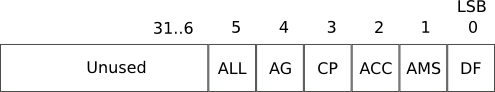
\includegraphics[width=4in]{figure/mobilec_threads_bitfields.png} 
  
  with the following acronyms:
    \begin{itemize}
      \item LSB: Least SignificantBit
      \item DF: Directory Facilitator
      \item AMS: Agent Management System
      \item ACC: Agent Communication Channel
      \item CP: Command Prompt
      \item AG: Agent Threads
    \end{itemize}
    A value of ``1'' in a bitfield tells Mobile-C to enable a particular thread,
    and a value of ``0'' informs Mobile-C not to activate that thread upon
    startup. A set of enumerations are defined in libmc.h that define the macros 
    \texttt{MC\_THREAD\_DF, MC\_THREAD\_AMS}, \texttt{MC\_THREAD\_ACC, MC\_THREAD\_CP, MC\_THREAD\_AGENT},
    each representing the bit position of each thread. There is also a 
    special macro, \texttt{MC\_THREAD\_ALL}, which represents the total number of 
    types of threads in a Mobile-C agency. For instance, to disable
    the command prompt thread, the following code may be used:
    \begin{verbatim}
    options.threads &= ~(1 << MC_OPTIONS_CP);
    \end{verbatim}
    where \texttt{options} is a struct of type \texttt{MCAgencyOptions\_t}.

    Helper functions \texttt{MC\_SetThreadOn(), MC\_SetThreadsAllOn(),
    MC\_SetThreadOff(), MC\_SetThreadsAllOff()} are also provided to modify the
    threads to start. Please consult their repsective documentation pages for
    more information.

  \item \texttt{int default\_agent\_status;} : This is the default agent status
  to assign to all incoming agents. Valid agent status values are found in
  \texttt{libmc.h} under the enumeration \texttt{MC\_AgentStatus\_e}. Possible
  values are:
    \begin{itemize}
    \item \texttt{MC\_WAIT\_CH} : This denotes that the agent is waiting for the
    next available Ch interpereter so that it may execute. This is the default
    setting for all incoming agents.
    \item \texttt{MC\_WAIT\_MESSGSEND} : This agent status indicates that the
    agent has finished its local task, but still has more remote tasks remaining.
    An agent with this status is waiting to be handled by the ACC so that it may
    migrate to the location of its next task.
    \item \texttt{MC\_AGENT\_ACTIVE} : This indicates that the agent is currently
    executing.
    \item \texttt{MC\_AGENT\_NEUTRAL} : This indicates that the agent is not
    executing, but is also not waiting for service. The agent simply persists 
    in the agency. This option is also a popular default alternative to
    \texttt{MC\_WAIT\_CH} since incoming agents are not executed upon arrival.
    \item \texttt{MC\_AGENT\_FINISHED} : This agent status indicates that the
    agent has finished all of its tasks and is awaiting to be purged from the
    agency.
    \end{itemize}
  \item \texttt{int modified;} : This member field is unused.
  \item \texttt{int enable\_security;} : This indicates that the Mobile-C agency
  should enable the Mobile-C security processes. This member is off by default.
  \item \texttt{unsigned char passphrase[32]} : This is a character string a
  passphrase to decrypt the agency's private key. For more details about the
  Mobile-C security process, please refer to Chapter \ref{chap:Security}.
  \item \texttt{int stack\_size[MC\_THREAD\_ALL];} : (Unix only) This array of integers holds
  the stack size to allocate for each thread. For example, if the programmer
  knows in advance that all agents the agency will receive will be small, the
  programmer may limit the stack size of each agent thread to one kilobyte with
  the following line:
  \begin{verbatim}
  options.stack_size[MC_THREAD_AGENT] = 1024;
  \end{verbatim}
  Care should be taken when modifying stack sizes as it may cause instability
  in the system. 
  \item \texttt{char *known\_host\_filename;} : (Optional) This should point to
  a filename containing host names of known and trusted hosts. This file is only
  used if Mobile-C security is enabled.
  \item \texttt{char *priv\_key\_filename;} : (Optional) This should point to a
  string containing the filename of the agency's private key file. This is only
  used if Mobile-C security is enabled.
  \item \texttt{ChOptions\_t* ch\_options;} : This may be used to modify Ch 
  options for agency interpreters. Please refer to the Embedded Ch documentation
  for more information about \texttt{ChOptions\_t}.
\end{itemize}

\noindent
{\bf Example: Starting an agency with default options}\\
\noindent
{\footnotesize\verbatiminput{../demos/getting_started/hello_world/server.c}}

{\bf Example: Starting an agency with no command prompt}\\
\noindent
{\footnotesize\verbatiminput{../demos/FIPA_compliant_ACL_messages/fipa_test/client.c}}

\noindent
{\bf See Also}\\
MC\_End()

%\CPlot::\DataThreeD(), \CPlot::\DataFile(), \CPlot::\Plotting(), \plotxy().\\

\pagebreak
\rhead{\bf MC\_InitializeAgencyOptions()}
\noindent
\vspace{5pt}
\rule{6.5in}{0.015in}
\noindent
\phantomsection
{\LARGE \bf MC\_InitializeAgencyOptions()\index{MC\_InitializeAgencyOptions()}}\\
\addcontentsline{toc}{section}{MC\_InitializeAgencyOptions()}
\label{api:MC_InitializeAgencyOptions()}

\noindent
{\bf Synopsis}\\
{\bf \#include $<$libmc.h$>$}\\
{\bf int MC\_InitializeAgencyOptions}({\bf struct MCAgencyOptions\_s* } options);\\

\noindent
{\bf Purpose}\\
Initialize the agency options structure to default values. \\

\noindent
{\bf Return Value}\\
The function returns 0 on success and non-zero otherwise.\\

\noindent
{\bf Parameters}
\vspace{-0.1in}
\begin{description}
\item
\begin{tabular}{p{10 mm}p{145 mm}} 
$options$ & An uninitialized reference to a \texttt{struct MCAgencyOptions\_s} type variable.
\end{tabular}
\end{description}

\noindent
{\bf Description}\\
This function fills the agency options struct with default values. This
function will overwrite any values that have already been set in the
struct. \\

\noindent
{\bf Example}\\
\noindent
{\footnotesize\verbatiminput{../demos/miscellaneous/mc_sample_app/mc_sample_app.c}}

\noindent
{\bf See Also}\\
MC\_Initialize().

%\CPlot::\DataThreeD(), \CPlot::\DataFile(), \CPlot::\Plotting(), \plotxy().\\

\pagebreak
\rhead{\bf MC\_LoadAgentFromFile()}
\noindent
\vspace{5pt}
\rule{6.5in}{0.015in}
\noindent
\phantomsection
{\LARGE \bf MC\_LoadAgentFromFile()\index{MC\_LoadAgentFromFile()}}\\
\addcontentsline{toc}{section}{MC\_LoadAgentFromFile()}
\label{api:MC_LoadAgentFromFile()}

\noindent
{\bf Synopsis}\\
{\bf \#include $<$libmc.h$>$}\\
{\bf int MC\_LoadAgentFromFile}({\bf MCAgency\_t} $agency$, {\bf const char*} $filename$);\\

\noindent
{\bf Purpose}\\
Add a mobile agent into a local agency from an XML file.\\

\noindent
{\bf Return Value}\\
The function returns 0 on success and non-zero otherwise.\\

\noindent
{\bf Parameters}
\vspace{-0.1in}
\begin{description}
\item
\begin{tabular}{p{10 mm}p{145 mm}} 
$agency$ & An initialized agency handle to add an agent to.\\
$filename$ & An xml file containing a MobileC mobile agent.
\end{tabular}
\end{description}

\noindent
{\bf Description}\\
This function adds a mobile agent to an agency. The agent is loaded from 
an xml file referenced by the \texttt{filename} function argument. \\

\noindent
{\bf Example}\\
\noindent
{\footnotesize\verbatiminput{../demos/communication_with_other_FIPA_compliant_agents/mc_to_jade_example/client.c}}

\noindent
{\bf See Also}\\

%\CPlot::\DataThreeD(), \CPlot::\DataFile(), \CPlot::\Plotting(), \plotxy().\\

\pagebreak
\rhead{\bf MC\_MainLoop()}
\noindent
\vspace{5pt}
\rule{6.5in}{0.015in}
\noindent
{\LARGE \bf MC\_MainLoop()\index{MC\_MainLoop()}}\\
\phantomsection
\addcontentsline{toc}{section}{MC\_MainLoop()}

\noindent
{\bf Synopsis}\\
{\bf \#include $<$libmc.h$>$}\\
{\bf int MC\_MainLoop}({\bf MCAgency\_t} $agency$);\\

\noindent
{\bf Purpose}\\
Cause the calling thread to wait indefinitely on an agency.\\

\noindent
{\bf Return Value}\\
If the Mobile-C agency is terminated safely from another 
thread or agent, the function will return 0. Otherwise, the function will
return a non-zero error code. \\

\noindent
{\bf Parameters}
\vspace{-0.1in}
\begin{description}
\item               
\begin{tabular}{p{10 mm}p{145 mm}}
$agency$ & A handle associated with a running agency. 
\end{tabular}
\end{description}

\noindent
{\bf Description}\\
This function will block the calling thread until another thread or agent
calls the function \texttt{MC\_End()} or \texttt{mc\_End()}, respectively.
This function will also stop blocking if the \texttt{quit} command is issued
from the Mobile-C command prompt.
It must be run on a handle that is attached to an agency that has already 
been started with the function \texttt{MC\_Initialize()}. Also note that 
it is not necessary to call this function to start a valid Mobile-C
agency. All agency threads and services are started upon calling
\texttt{MC\_Initialize()}, and \texttt{MC\_MainLoop()} is generally
only used to prevent the main thread from exiting.\\

\noindent
{\bf Example}\\
\noindent
{\footnotesize\verbatiminput{../demos/getting_started/hello_world/server.c}}

\noindent
{\bf See Also}\\

%\CPlot::\DataThreeD(), \CPlot::\DataFile(), \CPlot::\Plotting(), \plotxy().\\

\pagebreak
\rhead{\bf MC\_MigrateAgent()}
\noindent
\vspace{5pt}
\rule{6.5in}{0.015in}
\noindent
\phantomsection
{\LARGE \bf MC\_MigrateAgent()\index{MC\_MigrateAgent()}}\\
\addcontentsline{toc}{section}{MC\_MigrateAgent()}
\label{api:MC_MigrateAgent()}

\noindent
{\bf Synopsis}\\
{\bf \#include $<$libmc.h$>$}\\
{\bf int MC\_MigrateAgent}({\bf MCAgent\_t} $agent$, {\bf const char*} $hostname$, {\bf int} $port$);\\

\noindent
{\bf Purpose}\\
Instructs an agent to migrate to another host.\\

\noindent
{\bf Return Value}\\
The function returns 0 on success and non-zero otherwise.\\

\noindent
{\bf Parameters}
\vspace{-0.1in}
\begin{description}
\item
\begin{tabular}{p{15 mm}p{145 mm}} 
$agent$ & An initialized mobile agent. \\
$hostname$ & The new host to migrate to. \\
$port$ & The port on the new host to migrate to. \\
\end{tabular}
\end{description}

\noindent
{\bf Description}\\
This function instructs an agent to migrate to a new host. The task of the
agent is not incremented. The agent will executed whatever task it was
currently on when this function was invoked on the new host. Note that this
function only prepends a task to the agents task list. The agent still needs
to finish before the migration step occurs.\\

\noindent
{\bf Example}\\

\noindent
{\bf See Also}\\
mc\_MigrateAgent()

%\CPlot::\DataThreeD(), \CPlot::\DataFile(), \CPlot::\Plotting(), \plotxy().\\

\pagebreak
\rhead{\bf MC\_MutexLock()}
\noindent
\vspace{5pt}
\rule{6.5in}{0.015in}
\noindent
\phantomsection
{\LARGE \bf MC\_MutexLock()\index{MC\_MutexLock()}}\\
\addcontentsline{toc}{section}{MC\_MutexLock()}
\label{api:MC_MutexLock()}

\noindent
{\bf Synopsis}\\
{\bf \#include $<$libmc.h$>$}\\
{\bf int MC\_MutexLock}({\bf MCAgency\_t} agency, {\bf int} $id$);\\

\noindent
{\bf Purpose}\\
This function locks a previously initialized Mobile-C synchronization variable 
as a mutex. 
If the mutex is already locked, the function blocks until it is
unlocked before locking the mutex and continuing. \\

\noindent
{\bf Return Value}\\
This function returns 0 on success, or non-zero if the id could not be found. \\

\noindent
{\bf Parameters}
\vspace{-0.1pt}
\begin{description}
\item
\begin{tabular}{p{10 mm}p{145 mm}} 
$agency$ & The agency in which to find the synchronization variable to lock.\\
$id$ & The id of the synchronization variable to lock. 
\end{tabular}
\end{description}

\noindent
{\bf Description}\\
This function locks the mutex part of a Mobile-C synchronization variable. 
While this is primarily used to guard a shared resource, the behaviour is 
similar to the standard POSIX mutex locking. 
Note that although a MobileC synchronization variable may assume the role of a 
mutex, condition variable, or semaphore, once a Mobile-C synchronization 
variable is used as a mutex, it should not be used as anything else for the 
rest of its life cycle.\\ 

\noindent
{\bf Example}\\
Please see Program \vref{prog:binary_sync_example_server} in 
Chapter \ref{chap:synchronization}.\\

\noindent

\noindent
{\bf See Also}\\
MC\_MutexUnlock(), MC\_SyncInit(), MC\_SyncDelete().\\

%\CPlot::\DataThreeD(), \CPlot::\DataFile(), \CPlot::\Plotting(), \plotxy().\\

\pagebreak
\rhead{\bf MC\_MutexUnlock()}
\noindent
\vspace{5pt}
\rule{6.5in}{0.015in}
\noindent
\phantomsection
{\LARGE \bf MC\_MutexUnlock()\index{MC\_MutexUnlock()}}\\
\addcontentsline{toc}{section}{MC\_MutexUnlock()}

\noindent
{\bf Synopsis}\\
{\bf \#include $<$libmc.h$>$}\\
{\bf int MC\_MutexUnlock}({\bf MCAgency\_t} agency, {\bf int} $id$);\\

\noindent
{\bf Purpose}\\
This function unlocks a locked Mobile-C synchronization variable.\\

\noindent
{\bf Return Value}\\
This function returns 0 on success, or non-zero if the id could not be found.\\

\noindent
{\bf Parameters}
\vspace{-0.1pt}
\begin{description}
\item
\begin{tabular}{p{10 mm}p{145 mm}} 
$agency$ & The agency in which to find the synchronization variable to lock.\\
$id$ & The id of the synchronization variable to lock. 
\end{tabular}
\end{description}

\noindent
{\bf Description}\\
This function unlocks a Mobile-C synchronization variable that was previously
locked as a mutex. 
If the mutex is not locked while calling this function, undefined behaviour 
results.
Note that although a Mobile-C may act as a mutex, condition variable, or 
semaphore, once it has been locked and/or unlocked as a mutex, it should only 
be used as a mutex for the remainder of it's life cycle or unexpected 
behaviour may result.\\

\noindent
{\bf Example}\\
Please see Program \vref{prog:binary_sync_example_server} in 
Chapter \ref{chap:synchronization}.\\
\noindent
%Compare with output for examples in \CPlot::\Arrow(), \CPlot::\AutoScale(),
%\CPlot::\DisplayTime(), \CPlot::\Label(), \CPlot::\TicsLabel(), 
%\CPlot::\Margins(), \CPlot::\BoundingBoxOffsets(), \CPlot::\TicsDirection(),\linebreak
%\CPlot::\TicsFormat(), and \CPlot::\Title().
%{\footnotesize\verbatiminput{template/example/Data2D.ch}}

\noindent
{\bf See Also}\\
MC\_MutexLock(), MC\_SyncInit(), MC\_SyncDelete().\\

%\CPlot::\DataThreeD(), \CPlot::\DataFile(), \CPlot::\Plotting(), \plotxy().\\

\pagebreak
\rhead{\bf MC\_PrintAgentCode()}
\noindent
\vspace{5pt}
\rule{6.5in}{0.015in}
\noindent
{\LARGE \bf MC\_PrintAgentCode()\index{MC\_PrintAgentCode()}}\\
\phantomsection
\addcontentsline{toc}{section}{MC\_PrintAgentCode()}

\noindent
{\bf Synopsis}\\
{\bf \#include $<$libmc.h$>$}\\
{\bf int MC\_PrintAgentCode}({\bf MCAgent\_t} $agent$);\\

\noindent
{\bf Purpose}\\
Print a mobile agent code for inspection.\\

\noindent
{\bf Return Value}\\
The function returns 0 on success and non-zero otherwise.\\

\noindent
{\bf Parameters}
\vspace{-0.1in}
\begin{description}
\item               
\begin{tabular}{p{10 mm}p{145 mm}}
$agent$ & The mobile agent from which to print the code.
\end{tabular}
\end{description}

\noindent
{\bf Description}\\
This function prints the mobile agent code to the standard output.\\

\noindent
{\bf Example}\\
\noindent
%Compare with output for examples in \CPlot::\Arrow(), \CPlot::\AutoScale(),
%\CPlot::\DisplayTime(), \CPlot::\Label(), \CPlot::\TicsLabel(), 
%\CPlot::\Margins(), \CPlot::\BoundingBoxOffsets(), \CPlot::\TicsDirection(),\linebreak
%\CPlot::\TicsFormat(), and \CPlot::\Title().
%{\footnotesize\verbatiminput{template/example/Data2D.ch}}

\noindent
{\bf See Also}\\

%\CPlot::\DataThreeD(), \CPlot::\DataFile(), \CPlot::\Plotting(), \plotxy().\\

\pagebreak
\rhead{\bf MC\_RegisterService()}
\noindent
\vspace{5pt}
\rule{6.5in}{0.015in}
\noindent
\phantomsection
{\LARGE \bf MC\_RegisterService()\index{MC\_RegisterService()}}\\
\addcontentsline{toc}{section}{MC\_RegisterService()}
\label{api:MC_RegisterService()}

\noindent
{\bf Synopsis}\\
{\bf \#include $<$libmc.h$>$}\\
{\bf int MC\_RegisterService}({\bf MCAgency\_t} $agency$, {\bf MCAgent\_t} $agent$, {\bf int} agentID, {\bf const char} agentName, {\bf char**} serviceNames, {\bf int} numServices);\\

\noindent
{\bf Purpose}\\
Registers an agent service with an agency Directory Facilitator.\\

\noindent
{\bf Return Value}\\
The function returns 0 on success and non-zero otherwise.\\

\noindent
{\bf Parameters}
\vspace{-0.1in}
\begin{description}
\item
\begin{tabular}{p{23 mm}p{145 mm}} 
$agency$ & An initialized agency handle to add an agent to.\\
$agent$ & (Optional) An initialized mobile agent. \\
$agentID$ & (Optional) An agent id. \\
$agentName$ & (Optional) An agent name. \\
$serviceNames$ & A list of descriptive names for agent services. \\
$numServices$ & The number of services listed in the previous argument.
\end{tabular}
\end{description}

\noindent
{\bf Description}\\
This function is used to register agent services with an agency. Among
the optional arguments, either a valid agent must be supplied, or both
an agent ID and an agent name. Thus, services may be registered to an
agent which has not yet arrived at an agency by specifying the ID and name
of the agent.\\

\noindent
{\bf Example}\\
\noindent
{\footnotesize\verbatiminput{../demos/agent_space_functionality/mc_df_example/agent1.xml}}

\noindent
{\bf See Also}\\
mc\_RegisterService(), MC\_DeregisterService().

%\CPlot::\DataThreeD(), \CPlot::\DataFile(), \CPlot::\Plotting(), \plotxy().\\

\pagebreak
\rhead{\bf MC\_ResetSignal()}
\noindent
\vspace{5pt}
\rule{6.5in}{0.015in}
\noindent
{\LARGE \bf MC\_ResetSignal()\index{MC\_ResetSignal()}}\\
\phantomsection
\addcontentsline{toc}{section}{MC\_ResetSignal()}

\noindent
{\bf Synopsis}\\
{\bf \#include $<$libmc.h$>$}\\
{\bf int MC\_ResetSignal}({\bf MCAgency\_t} $agency$);\\

\noindent
{\bf Purpose}\\
This function is used to reset the Mobile-C signalling system. 
It is intended to be used after returning from a call to function 
{\bf MC\_WaitSignal()}.\\

\noindent
{\bf Return Value}\\
This function returns 0 on success and non-zero otherwise.\\

\noindent
{\bf Parameters}
\vspace{-0.1in}
\begin{description}
\item               
\begin{tabular}{p{10 mm}p{145 mm}}
$agency$ & A handle to a running agency.
\end{tabular}
\end{description}

\noindent
{\bf Description}\\
This function is used to reset the Mobile-C signalling system. 
System signals are triggered by certain events in the Mobile-C library. 
This includes events such as the arrival of a new message or mobile agent, and 
the departure of a mobile agent, etc. 
If function {\bf MC\_WaitSignal()} is used to listen for one of these events, 
function {\bf MC\_ResetSignal()} must be called in order to allow Mobile-C to 
resume with it's operations.\\

\noindent
{\bf Example}\\
\noindent
{\footnotesize\verbatiminput{../demos/composing_agents/multi_task_example/client.c}}

\noindent
{\bf See Also}\\
MC\_WaitSignal() \\

%\CPlot::\DataThreeD(), \CPlot::\DataFile(), \CPlot::\Plotting(), \plotxy().\\

\pagebreak
\rhead{\bf MC\_ResumeAgency()}
\noindent
\vspace{5pt}
\rule{6.5in}{0.015in}
\noindent
\phantomsection
{\LARGE \bf MC\_ResumeAgency()\index{MC\_ResumeAgency()}}\\
\addcontentsline{toc}{section}{MC\_ResumeAgency()}
\label{api:MC_ResumeAgency()}

\noindent
{\bf Synopsis}\\
{\bf \#include $<$libmc.h$>$}\\
{\bf int MC\_ResumeAgency}({\bf MCAgency\_t} $agency$);\\

\noindent
{\bf Purpose}\\
This function resumes the execution of an agency. \\

\noindent
{\bf Return Value}\\
The function returns 0 on success and non-zero otherwise.\\

\noindent
{\bf Parameters}
\vspace{-0.1in}
\begin{description}
\item
\begin{tabular}{p{10 mm}p{145 mm}} 
$agency$ & An initialized agency handle. 
\end{tabular}
\end{description}

\noindent
{\bf Description}\\
This function resumes the operation of the core threads of the Mobile-C
agency, such as the ACC, AMS, etc., after they have been halted by the 
\texttt{MC\_HaltAgency()} function.\\

\noindent
{\bf Example}\\
\noindent
% FIXME: Need an example here
%{\footnotesize\verbatiminput{../demos/multiple_agency_example/server.c}}

\noindent
{\bf See Also}\\
MC\_HaltAgency().

%\CPlot::\DataThreeD(), \CPlot::\DataFile(), \CPlot::\Plotting(), \plotxy().\\

\pagebreak
\rhead{\bf MC\_RetrieveAgent()}
\noindent
\vspace{5pt}
\rule{6.5in}{0.015in}
\noindent
{\LARGE \bf MC\_RetrieveAgent()\index{MC\_RetrieveAgent()}}\\
\phantomsection
\addcontentsline{toc}{section}{MC\_RetrieveAgent()}

\noindent
{\bf Synopsis}\\
{\bf \#include $<$libmc.h$>$}\\
{\bf MCAgent\_t MC\_RetrieveAgent}({\bf MCAgency\_t} $agency$);\\

\noindent
{\bf Purpose}\\
Retrieve the first neutral mobile agent from a mobile agent list.\\

\noindent
{\bf Return Value}\\
The function returns an {\bf MCAgent\_t} object on success or NULL on failure.\\

\noindent
{\bf Parameters}
\vspace{-0.1in}
\begin{description}
\item               
\begin{tabular}{p{10 mm}p{145 mm}}
$agency$ & An agency handle.\\
\end{tabular}
\end{description}

\noindent
{\bf Description}\\
This function retrieves the first agent with status MC\_AGENT\_NEUTRAL from a 
mobile agent list. 
If there are no mobile agents with this attribute, the return value is NULL.\\

\noindent
{\bf Example}\\
\noindent
%Compare with output for examples in \CPlot::\Arrow(), \CPlot::\AutoScale(),
%\CPlot::\DisplayTime(), \CPlot::\Label(), \CPlot::\TicsLabel(), 
%\CPlot::\Margins(), \CPlot::\BoundingBoxOffsets(), \CPlot::\TicsDirection(),\linebreak
%\CPlot::\TicsFormat(), and \CPlot::\Title().
%{\footnotesize\verbatiminput{template/example/Data2D.ch}}

\noindent
{\bf See Also}\\

%\CPlot::\DataThreeD(), \CPlot::\DataFile(), \CPlot::\Plotting(), \plotxy().\\

\pagebreak
\rhead{\bf MC\_RetrieveAgentCode()}
\noindent
\vspace{5pt}
\rule{6.5in}{0.015in}
\noindent
{\LARGE \bf MC\_RetrieveAgentCode()\index{MC\_RetrieveAgentCode()}}\\
\phantomsection
\addcontentsline{toc}{section}{MC\_RetrieveAgentCode()}
\label{api:MC_RetrieveAgentCode()}

\noindent
{\bf Synopsis}\\
{\bf \#include $<$libmc.h$>$}\\
{\bf char *MC\_RetrieveAgentCode}({\bf MCAgent\_t} $agent$);\\

\noindent
{\bf Purpose}\\
Retrieve a mobile agent code in the form of a character string.\\

\noindent
{\bf Return Value}\\
The function returns an allocated character array on success and NULL on 
failure.\\

\noindent
{\bf Parameters}
\vspace{-0.1in}
\begin{description}
\item               
\begin{tabular}{p{10 mm}p{145 mm}}
$agent$ & The mobile agent from which to retrieve the code.
\end{tabular}
\end{description}

\noindent
{\bf Description}\\
This function retrieves a mobile agent code. 
The return pointer is allocated by 'malloc()' and must be freed by the user.\\

\noindent
{\bf Example}\\
\noindent
{\footnotesize\verbatiminput{../demos/mobilec_c-space_functionality/cspace_misc_examples/server.c}}

\noindent
{\bf See Also}\\

%\CPlot::\DataThreeD(), \CPlot::\DataFile(), \CPlot::\Plotting(), \plotxy().\\

\pagebreak
\rhead{\bf MC\_SearchForService()}
\noindent
\vspace{5pt}
\rule{6.5in}{0.015in}
\noindent
\phantomsection
{\LARGE \bf MC\_SearchForService()\index{MC\_SearchForService()}}\\
\addcontentsline{toc}{section}{MC\_SearchForService()}
\label{api:MC_SearchForService()}

\noindent
{\bf Synopsis}\\
{\bf \#include $<$libmc.h$>$}\\
{\bf int MC\_SearchForService}({\bf MCAgency\_t} $agency$, {\bf char*} SearchString,  {\bf char***} $agentNames$, {\bf char***} serviceNames, {\bf int **} agentIDs,{\bf int*} numResults);\\

\noindent
{\bf Purpose}\\
Searches the Directory Facilitator for a service.\\

\noindent
{\bf Return Value}\\
The function returns 0 on success and non-zero otherwise.\\

\noindent
{\bf Parameters}
\vspace{-0.1in}
\begin{description}
\item
\begin{tabular}{p{23 mm}p{145 mm}} 
$agency$ & An initialized agency handle.\\
$searchString$ & (in) A search substring. All services names registered with the Directory Facilitator with a matching substring will be a hit. \\
$agentNames$ & (out) A newly allocated array of agent names of agents that provide services matching the search string. \\
$serviceNames$ & (out) A newly allocated array of service names matching the search substring. \\
$AgentIDs$ & (out) A newly allocated array of agent IDs of matching agents. \\
$numServices$ & (out) The number of services listed in the previous argument.
\end{tabular}
\end{description}

\noindent
{\bf Description}\\
This function is used to search the Directory Facilitator for a service.
The function will return all services if any part of the service name 
matches the search string. \\

\noindent
{\bf Example}\\
\noindent
{\footnotesize\verbatiminput{../demos/agent_space_functionality/mc_df_example/agent3.xml}}

\noindent
{\bf See Also}\\
MC\_RegisterService(), MC\_DeregisterService().

%\CPlot::\DataThreeD(), \CPlot::\DataFile(), \CPlot::\Plotting(), \plotxy().\\

\pagebreak
\rhead{\bf MC\_SemaphorePost()}
\noindent
\vspace{5pt}
\rule{6.5in}{0.015in}
\noindent
\phantomsection
{\LARGE \bf MC\_SemaphorePost()\index{MC\_SemaphorePost()}}\\
\addcontentsline{toc}{section}{MC\_SemaphorePost()}

\noindent
{\bf Synopsis}\\
{\bf \#include $<$libmc.h$>$}\\
{\bf int MC\_SemaphorePost}({\bf MCAgency\_t} agency, {\bf int} $id$);\\

\noindent
{\bf Purpose}\\
This function unlocks one resource from a Mobile-C semaphore, increasing its
count by one.\\

\noindent
{\bf Return Value}\\
This function returns 0 on success, or non-zero if the id could not be found 
or on a semaphore error.\\

\noindent
{\bf Parameters}
\vspace{-0.1pt}
\begin{description}
\item
\begin{tabular}{p{10 mm}p{145 mm}} 
$agency$ & The agency in which to find the synchronization variable to lock.\\
$id$ & The id of the synchronization variable to lock. 
\end{tabular}
\end{description}

\noindent
{\bf Description}\\
{\bf MC\_SemaphorePost} unlocks a resourse from a previously allocated and 
initialized Mobile-C synchronization variable being used as a semaphore. 
This function may be called multiple times to increase the count of the 
semaphore up to INT\_MAX. 
Note that although a Mobile-C synchronization variable may be used as a mutex, 
condition variable, or semaphore, once it is used as a semaphore, it should 
only be used as a semaphore for the remainder of its life cycle.\\

\noindent
{\bf Example}\\
The MC\_SemaphorePost() function usage is very similar to the other
binary space synchronization functions. Please see Chapter 
\ref{chap:synchronization} on page \pageref{chap:synchronization} 
and the demo at ``demos/agent\_semaphore\_example/'' for
more information.\\
\noindent
%Compare with output for examples in \CPlot::\Arrow(), \CPlot::\AutoScale(),
%\CPlot::\DisplayTime(), \CPlot::\Label(), \CPlot::\TicsLabel(), 
%\CPlot::\Margins(), \CPlot::\BoundingBoxOffsets(), \CPlot::\TicsDirection(),\linebreak
%\CPlot::\TicsFormat(), and \CPlot::\Title().
%{\footnotesize\verbatiminput{template/example/Data2D.ch}}

\noindent
{\bf See Also}\\
MC\_SemaphoreWait(), MC\_SyncInit(), MC\_SyncDelete().\\

%\CPlot::\DataThreeD(), \CPlot::\DataFile(), \CPlot::\Plotting(), \plotxy().\\

\pagebreak
\rhead{\bf MC\_SemaphoreWait()}
\noindent
\vspace{5pt}
\rule{6.5in}{0.015in}
\noindent
\phantomsection
{\LARGE \bf MC\_SemaphoreWait()\index{MC\_SemaphoreWait()}}\\
\addcontentsline{toc}{section}{MC\_SemaphoreWait()}

\noindent
{\bf Synopsis}\\
{\bf \#include $<$libmc.h$>$}\\
{\bf int MC\_SemaphoreWait}({\bf MCAgency\_t} agency, {\bf int} $id$);\\

\noindent
{\bf Purpose}\\
This function allocates one resource from a Mobile-C synchronization semaphore 
variable.\\

\noindent
{\bf Return Value}\\
This function returns 0 on success, or non-zero if the id could not be found.\\

\noindent
{\bf Parameters}
\vspace{-0.1pt}
\begin{description}
\item
\begin{tabular}{p{10 mm}p{145 mm}} 
$agency$ & The agency in which to find the synchronization variable to lock.\\
$id$ & The id of the synchronization variable to lock. 
\end{tabular}
\end{description}

\noindent
{\bf Description}\\
This function allocates one resource from a previously allocated and 
initialized Mobile-C synchronization semaphore. 
If the semaphore resource count is non-zero, the resource is immediately 
allocated. 
If the semaphore resource count is zero, the function blocks until a resource 
is freed before allocating a resource and continuing. 
Note that although a Mobile-C synchronization variable may be used as a mutex, 
condition variable, or semaphore, once it is used as a semaphore, it should 
only be used as a semaphore for the remainder of its life cycle.\\

\noindent
{\bf Example}\\
The MC\_SemaphorePost() function usage is very similar to the other
binary space synchronization functions. Please see Chapter 
\ref{chap:synchronization} on page \pageref{chap:synchronization} for
more information.\\
\noindent
%Compare with output for examples in \CPlot::\Arrow(), \CPlot::\AutoScale(),
%\CPlot::\DisplayTime(), \CPlot::\Label(), \CPlot::\TicsLabel(), 
%\CPlot::\Margins(), \CPlot::\BoundingBoxOffsets(), \CPlot::\TicsDirection(),\linebreak
%\CPlot::\TicsFormat(), and \CPlot::\Title().
%{\footnotesize\verbatiminput{template/example/Data2D.ch}}

\noindent
{\bf See Also}\\
MC\_SemaphorePost(), MC\_SyncInit(), MC\_SyncDelete().\\

%\CPlot::\DataThreeD(), \CPlot::\DataFile(), \CPlot::\Plotting(), \plotxy().\\

\pagebreak
\rhead{\bf MC\_SendAgent()}
\noindent
\vspace{5pt}
\rule{6.5in}{.01in}
\noindent
{\LARGE \bf MC\_SendAgent()\index{MC\_SendAgent()}} \\
\phantomsection
\addcontentsline{toc}{section}{MC\_SendAgent()}

\noindent
{\bf Synopsis}\\
{\bf \#include $<$libmc.h$>$}\\
{\bf int MC\_SendAgent}({\bf MCAgency\_t} $agency$, {\bf char *}$message$);\\

\noindent
{\bf Purpose}\\
Send an ACL mobile agent message to a remote agency.

\noindent
{\bf Return Value}\\
The function returns 0 on success and non-zero otherwise.\\

\noindent
{\bf Parameters}
\vspace{-0.1in}
\begin{description}
\item
\begin{tabular}{p{20 mm}p{135 mm}}
$agency$ & A handle associated with an agency from which to send the ACL 
mobile agent message. A NULL pointer can be used to send the ACL message 
from an unspecified agency.\\ 
$message$ & The ACL mobile agent message to be sent.\\
\end{tabular}
\end{description}

\noindent
{\bf Description}\\
This function is used to send an XML based ACL mobile agent message, which 
is a string, to a remote agency. \\

\noindent
{\bf Example}\\
\noindent
%Compare with output for examples in \CPlot::\Arrow(), \CPlot::\AutoScale(),
%\CPlot::\DisplayTime(), \CPlot::\Label(), \CPlot::\TicsLabel(), 
%\CPlot::\Margins(), \CPlot::\BoundingBoxOffsets(), \CPlot::\TicsDirection(),\linebreak
%\CPlot::\TicsFormat(), and \CPlot::\Title().
%{\footnotesize\verbatiminput{template/example/Data2D.ch}}

\noindent
{\bf See Also}\\

%\CPlot::\DataThreeD(), \CPlot::\DataFile(), \CPlot::\Plotting(), \plotxy().\\

\pagebreak
\rhead{\bf MC\_SendAgentFile()} 
\noindent
\vspace{5pt}
\rule{6.5in}{.01in}
\noindent
{\LARGE \bf MC\_SendAgentFile()\index{MC\_SendAgentFile()}}\\ 
\phantomsection
\addcontentsline{toc}{section}{MC\_SendAgentFile()}
\label{api:MC_SendAgentFile()}

\noindent
{\bf Synopsis}\\
{\bf \#include $<$libmc.h$>$}\\
{\bf int MC\_SendAgentFile}({\bf MCAgency\_t} $agency$, {\bf char *}$filename$);\\

\noindent
{\bf Purpose}\\
Send an ACL mobile agent message saved as a file to a remote agency.

\noindent
{\bf Return Value}\\
The function returns 0 on success and non-zero otherwise.\\

\noindent
{\bf Parameters}
\vspace{-0.1in}
\begin{description}
\item
\begin{tabular}{p{20 mm}p{135 mm}}
$agency$ & A handle associated with an agency from which to send the ACL 
mobile agent message. A NULL pointer can be used to send the ACL message 
from an unspecified agency.\\ 
$filename$ & The ACL mobile agent message file to be sent.\\
\end{tabular}
\end{description}

\noindent
{\bf Description}\\
This function is used to send an XML based ACL mobile agent message, which 
is saved as a file, to a remote agency. \\

\noindent
{\bf Example}\\
\noindent
{\footnotesize\verbatiminput{../demos/getting_started/hello_world/client.c}}

\noindent
{\bf See Also}\\

%\CPlot::\DataThreeD(), \CPlot::\DataFile(), \CPlot::\Plotting(), \plotxy().\\

\pagebreak
\rhead{\bf MC\_SendAgentMigrationMessage()}
\noindent
\vspace{5pt}
\rule{6.5in}{.01in}
\noindent
{\LARGE \bf MC\_SendAgentMigrationMessage()\index{MC\_SendAgentMigrationMessage()}} [Deprecated] \\
\phantomsection
\addcontentsline{toc}{section}{MC\_SendAgentMigrationMessage()}

\noindent
{\bf Synopsis}\\
{\bf \#include $<$libmc.h$>$}\\
{\bf int MC\_SendAgentMigrationMessage}({\bf MCAgency\_t} $agency$, {\bf char *}$message$, {\bf char *}$hostname$, {\bf int} $port$);\\

\noindent
{\bf Purpose}\\
Send an ACL mobile agent message to a remote agency.

Please note that this function is deprecated. Please use the
\texttt{MC\_SendAgent()} function instead.\\

\noindent
{\bf Return Value}\\
The function returns 0 on success and non-zero otherwise.\\

\noindent
{\bf Parameters}
\vspace{-0.1in}
\begin{description}
\item
\begin{tabular}{p{20 mm}p{135 mm}}
$agency$ & A handle associated with an agency from which to send the ACL 
mobile agent message. A NULL pointer can be used to send the ACL message 
from an unspecified agency.\\ 
$message$ & The ACL mobile agent message to be sent.\\
$hostname$ & The hostname of the remote agency. It can be in number-dot 
format or hostname format, i.e., 169.237.104.199 or machine.ucdavis.edu.\\
$port$ & The port number on which the remote agency is listening. 
\end{tabular}
\end{description}

\noindent
{\bf Description}\\
This function is used to send an XML based ACL mobile agent message, which 
is a string, to a remote agency. 
This function can be used without a running local agency.\\

\noindent
{\bf Example}\\
\noindent
%Compare with output for examples in \CPlot::\Arrow(), \CPlot::\AutoScale(),
%\CPlot::\DisplayTime(), \CPlot::\Label(), \CPlot::\TicsLabel(), 
%\CPlot::\Margins(), \CPlot::\BoundingBoxOffsets(), \CPlot::\TicsDirection(),\linebreak
%\CPlot::\TicsFormat(), and \CPlot::\Title().
%{\footnotesize\verbatiminput{template/example/Data2D.ch}}

\noindent
{\bf See Also}\\

%\CPlot::\DataThreeD(), \CPlot::\DataFile(), \CPlot::\Plotting(), \plotxy().\\

\pagebreak
\rhead{\bf MC\_SendAgentMigrationMessageFile()} 
\noindent
\vspace{5pt}
\rule{6.5in}{.01in}
\noindent
{\LARGE \bf MC\_SendAgentMigrationMessageFile()\index{MC\_SendAgentMigrationMessageFile()}} [Deprecated]\\ 
\phantomsection
\addcontentsline{toc}{section}{MC\_SendAgentMigrationMessageFile()}
\label{api:MC_SendAgentMigrationMessageFile()}

\noindent
{\bf Synopsis}\\
{\bf \#include $<$libmc.h$>$}\\
{\bf int MC\_SendAgentMigrationMessageFile}({\bf MCAgency\_t} $agency$, {\bf char *}$filename$, {\bf char *}$hostname$, {\bf int} $port$);\\

\noindent
{\bf Purpose}\\
Send an ACL mobile agent message saved as a file to a remote agency.

Please note that this function is deprecated. Please use the
\texttt{MC\_SendAgentFile()} function instead.\\

\noindent
{\bf Return Value}\\
The function returns 0 on success and non-zero otherwise.\\

\noindent
{\bf Parameters}
\vspace{-0.1in}
\begin{description}
\item
\begin{tabular}{p{20 mm}p{135 mm}}
$agency$ & A handle associated with an agency from which to send the ACL 
mobile agent message. A NULL pointer can be used to send the ACL message 
from an unspecified agency.\\ 
$filename$ & The ACL mobile agent message file to be sent.\\
$hostname$ & The hostname of the remote agency. It can be in number-dot 
format or hostname format, i.e., 169.237.104.199 or machine.ucdavis.edu.\\
$port$ & The port number on which the remote agency is listening. 
\end{tabular}
\end{description}

\noindent
{\bf Description}\\
This function is used to send an XML based ACL mobile agent message, which 
is saved as a file, to a remote agency. 
This function can be used without a running local agency.\\

\noindent
{\bf Example}\\
\noindent
{\footnotesize\verbatiminput{../demos/getting_started/hello_world/client.c}}

\noindent
{\bf See Also}\\

%\CPlot::\DataThreeD(), \CPlot::\DataFile(), \CPlot::\Plotting(), \plotxy().\\

\pagebreak
\rhead{\bf MC\_SendSteerCommand()}
\noindent
\vspace{5pt}
\rule{6.5in}{0.015in}
\noindent
\phantomsection
{\LARGE \bf MC\_SendSteerCommand()\index{MC\_SendSteerCommand()}}\\
\addcontentsline{toc}{section}{MC\_SendSteerCommand()}
\label{api:MC_SendSteerCommand()}

\noindent
{\bf Synopsis}\\
{\bf \#include $<$libmc.h$>$}\\
{\bf int MC\_SendSteerCommand}({\bf MCAgency\_t} $agency$, {\bf enum MC\_SteerCommand\_e} cmd);\\

\noindent
{\bf Purpose}\\
Send a steering command to a Mobile-C computational steering algorithm.\\

\noindent
{\bf Return Value}\\
The function returns 0 on success and non-zero otherwise.\\

\noindent
{\bf Parameters}
\vspace{-0.1in}
\begin{description}
\item
\begin{tabular}{p{10 mm}p{145 mm}} 
$agency$ & An initialized agency handle to add an agent to.\\
$cmd$ & The command to send.
\end{tabular}
\end{description}

\noindent
{\bf Description}\\
This function sends a steering command to a Mobile-C steerable algorithm.

\noindent
{\bf Example}\\
\noindent
{\footnotesize\verbatiminput{../demos/miscellaneous/steer_example/suspend.xml}}

\noindent
{\bf See Also}\\
MC\_Steer(), MC\_SteerControl().

%\CPlot::\DataThreeD(), \CPlot::\DataFile(), \CPlot::\Plotting(), \plotxy().\\

\pagebreak
\rhead{\bf MC\_SetAgentStatus()}
\noindent
\vspace{5pt}
\rule{6.5in}{0.015in}
\noindent
{\LARGE \bf MC\_SetAgentStatus()\index{MC\_SetAgentStatus()}}\\
\phantomsection
\addcontentsline{toc}{section}{MC\_SetAgentStatus()}
\label{api:MC_SetAgentStatus()}

\noindent
{\bf Synopsis}\\
{\bf \#include $<$libmc.h$>$}\\
{\bf int MC\_SetAgentStatus}({\bf MCAgent\_t} $agent$, {\bf int} $status$);\\

\noindent
{\bf Purpose}\\
Set the status of a mobile agent in an agency.\\

\noindent
{\bf Return Value}\\
This function returns 0 on success and non-zero otherwise.\\

\noindent
{\bf Parameters}
\vspace{-0.1in}
\begin{description}
\item               
\begin{tabular}{p{10 mm}p{145 mm}}
$agent$ & The mobile agent whose status is to be assigned.\\
$status$ & An integer representing the status to be assinged to a mobile agent.
\end{tabular}
\end{description}

\noindent
{\bf Description}\\
This function returns an integer of enumerated type
{\texttt enum MC\_AgentStatus\_e}. Details about this enumerated type may be
found in Table \ref{mobilec_macro} on page \pageref{mobilec_macro}.\\

\noindent
{\bf Example}\\
\noindent
{\footnotesize\verbatiminput{../demos/miscellaneous/multiple_agency_example/server.c}}

\noindent
{\bf See Also}\\

%\CPlot::\DataThreeD(), \CPlot::\DataFile(), \CPlot::\Plotting(), \plotxy().\\

\pagebreak
\rhead{\bf MC\_SetDefaultAgentStatus()}
\noindent
\vspace{5pt}
\rule{6.5in}{0.015in}
\noindent
{\LARGE \bf MC\_SetDefaultAgentStatus()\index{MC\_SetDefaultAgentStatus()}}\\
\phantomsection
\addcontentsline{toc}{section}{MC\_SetDefaultAgentStatus()}
\label{api:MC_SetDefaultAgentStatus()}

\noindent
{\bf Synopsis}\\
{\bf \#include $<$libmc.h$>$}\\
{\bf int MC\_SetDefaultAgentStatus}({\bf MCAgency\_t} $agency$, {\bf int} $status$);\\

\noindent
{\bf Purpose}\\
Set the default status of any incoming mobile agents.\\

\noindent
{\bf Return Value}\\
This function returns 0 on success and non-zero otherwise.\\

\noindent
{\bf Parameters}
\vspace{-0.1in}
\begin{description}
\item               
\begin{tabular}{p{10 mm}p{145 mm}}
$agency$ & A handle to a running agency.\\
$status$ & An integer representing the status to be assinged to any incoming 
mobile agents as their default status.
\end{tabular}
\end{description}

\noindent
{\bf Description}\\
This function is used to set the default agent status for all incoming
agents in an agency. By default, every incoming agent is set to status
``MC\_WAIT\_CH'', but that may be changed with this function.
The agent status is an enumerated type ``enum MC\_AgentStatus\_e'', which
may be seen in Table \vref{mobilec_macro}.

\noindent
{\bf Example}\\
\begin{verbatim}
MCAgency_t agency;
agency = MC_Initialize(5050, NULL);
MC_SetDefaultAgentStatus(agency, MC_AGENT_NEUTRAL);

/* etc... */
\end{verbatim}\\
\noindent
%Compare with output for examples in \CPlot::\Arrow(), \CPlot::\AutoScale(),
%\CPlot::\DisplayTime(), \CPlot::\Label(), \CPlot::\TicsLabel(), 
%\CPlot::\Margins(), \CPlot::\BoundingBoxOffsets(), \CPlot::\TicsDirection(),\linebreak
%\CPlot::\TicsFormat(), and \CPlot::\Title().
%{\footnotesize\verbatiminput{template/example/Data2D.ch}}

\noindent
{\bf See Also}\\
MC\_GetAgentStatus()


\pagebreak
\rhead{\bf MC\_SetThreadOff()}
\noindent
\vspace{5pt}
\rule{6.5in}{0.015in}
\noindent
{\LARGE \bf MC\_SetThreadOff()\index{MC\_SetThreadOff()}}\\
\phantomsection
\addcontentsline{toc}{section}{MC\_SetThreadOff()}

\noindent
{\bf Synopsis}\\
{\bf \#include $<$libmc.h$>$}\\
{\bf int MC\_SetThreadOff}({\bf MCAgencyOptions\_t} $*options$, {\bf enum threadIndex\_e} $thread$);\\

\noindent
{\bf Purpose}\\
Set a particular thread to not execute upon Mobile-C initialization.\\

\noindent
{\bf Return Value}\\
This function returns 0 on success and non-zero otherwise. \\

\noindent
{\bf Parameters}
\vspace{-0.1in}
\begin{description}
\item               
\begin{tabular}{p{10 mm}p{145 mm}}
$options$ & An allocated MCAgencyOptions\_t variable.\\
$thread$ & A thread index.
\end{tabular}
\end{description}

\noindent
{\bf Description}\\
This function is used to modify the Mobile-C startup options. 
It is used to disable threads that may otherwise be enabled. 
The threads which may be modified are
\vspace{-0.1in}
\begin{description}
\item               
\begin{tabular}{p{40 mm}p{125 mm}}
MC\_THREAD\_AI : & Agent Initializing Thread - Create agent from incoming messages.\\
MC\_THREAD\_AM : & Agent Managing Thread - Manage active agents.\\
MC\_THREAD\_CL : & Connection Listening Thread - Listen incoming connections.\\
MC\_THREAD\_MR : & Message Receiving Thread - Handle incoming connections and recieve agent messages.\\
MC\_THREAD\_MS : & Message Sending Thread - Handle outgoing connections and send agent messages.\\
MC\_THREAD\_CP : & Command Prompt Thread - Handle an interactive user command prompt.
\end{tabular}
\end{description}

\noindent
{\bf Example}\\
\begin{verbatim}
MCAgencyOptions_t options;
MCAgency_t agency;

/* Turn the listen thread off. We will receive our messages 
   in another method. */
MC_SetThreadOff(&options, MC_THREAD_AI);

/* Start the agency with no listen thread*/
agency = MC_Initialize(5050, &options);

/* etc ... */
\end{verbatim}

\noindent
{\bf See Also}\\
MC\_SetThreadOn()\\
%\CPlot::\DataThreeD(), \CPlot::\DataFile(), \CPlot::\Plotting(), \plotxy().\\


\pagebreak
\rhead{\bf MC\_SetThreadOn()}
\noindent
\vspace{5pt}
\rule{6.5in}{0.015in}
\noindent
{\LARGE \bf MC\_SetThreadOn()\index{MC\_SetThreadOn()}}\\
\phantomsection
\addcontentsline{toc}{section}{MC\_SetThreadOn()}

\noindent
{\bf Synopsis}\\
{\bf \#include $<$libmc.h$>$}\\
{\bf int MC\_SetThreadOn}({\bf MCAgencyOptions\_t} $*options$, {\bf enum threadIndex\_e} $thread$);\\

\noindent
{\bf Purpose}\\
Sets a particular thread to execute upon Mobile C initialization.\\

\noindent
{\bf Return Value}\\
This function returns 0 on success and non-zero otherwise.\\

\noindent
{\bf Parameters}
\vspace{-0.1in}
\begin{description}
\item               
\begin{tabular}{p{10 mm}p{145 mm}}
$options$ & An allocated MCAgencyOptions\_t variable.\\
$thread$ & A thread index.
\end{tabular}
\end{description}

\noindent
{\bf Description}\\
This function is used to modify the Mobile-C startup options. 
It is used to enable threads that may otherwise be disabled. 
The threads which may be modified are
\vspace{-0.1in}
\begin{description}
\item
\begin{tabular}{p{40 mm}p{125 mm}}
MC\_THREAD\_AI : & Agent Initializing Thread - Create agent from incoming messages.\\
MC\_THREAD\_AM : & Agent Managing Thread - Manage active agents.\\
MC\_THREAD\_CL : & Connection Listening Thread - Listen incoming connections.\\
MC\_THREAD\_MR : & Message Receiving Thread - Handle incoming connections and recieve agent messages.\\
MC\_THREAD\_MS : & Message Sending Thread - Handle outgoing connections and send agent messages.\\
MC\_THREAD\_CP : & Command Prompt Thread - Handle an interactive user command prompt.
\end{tabular}
\end{description}

\noindent
{\bf Example}\\
\noindent
\begin{verbatim}
MCAgencyOptions_t options;
MCAgency_t agency;

/* Turn the command prompt thread on */
MC_SetThreadOn(&options, MC_THREAD_CP);

/* Start the agency with a command prompt on port 5050 */
agency = MC_Initialize(5050, &options);

/* etc ... */
\end{verbatim}

\noindent
{\bf See Also}\\
MC\_SetThreadOff()\\
%\CPlot::\DataThreeD(), \CPlot::\DataFile(), \CPlot::\Plotting(), \plotxy().\\


\pagebreak
\rhead{\bf MC\_Steer()}
\noindent
\vspace{5pt}
\rule{6.5in}{0.015in}
\noindent
\phantomsection
{\LARGE \bf MC\_Steer()\index{MC\_Steer()}}\\
\addcontentsline{toc}{section}{MC\_Steer()}

\noindent
{\bf Synopsis}\\
{\bf \#include $<$libmc.h$>$}\\
{\bf int MC\_Steer}({\bf MCAgency\_t} attr, {\bf int} (*funcptr)({\bf void*} data), {\bf void*} arg);\\

\noindent
{\bf Purpose}\\
The MC\_Steer function initialized and runs a function containing an algorithm. 
The function enables the steering functionality of the algorithm so that it may accept 
command during runtime to change the execution of the algorithm. 
For more information, please see the example and the demo located in the 
demos/steer\_example/ directory.\\ 

\noindent
{\bf Return Value}\\
The function returns 0 on success, or a non-zero error code on failure. \\

\noindent
{\bf Description}\\
The {\bf MC\_Steer} function is designed execute an algorithm in a fashion which enables
that algorithm to be steered or modified on-the-fly during runtime. See the demo and
the example for more details. \\

\noindent
{\bf Example}\\
\noindent
{\footnotesize \verbatiminput{../demos/miscellaneous/steer_example/server.c}}
%Compare with output for examples in \CPlot::\Arrow(), \CPlot::\AutoScale(),
%\CPlot::\DisplayTime(), \CPlot::\Label(), \CPlot::\TicsLabel(), 
%\CPlot::\Margins(), \CPlot::\BoundingBoxOffsets(), \CPlot::\TicsDirection(),\linebreak
%\CPlot::\TicsFormat(), and \CPlot::\Title().
%{\footnotesize\verbatiminput{template/example/Data2D.ch}}

\noindent
{\bf See Also}\\
MC\_SteerControl()

%\CPlot::\DataThreeD(), \CPlot::\DataFile(), \CPlot::\Plotting(), \plotxy().\\

\pagebreak
\rhead{\bf MC\_SteerControl()}
\noindent
\vspace{5pt}
\rule{6.5in}{0.015in}
\noindent
\phantomsection
{\LARGE \bf MC\_SteerControl()\index{MC\_SteerControl()}}\\
\addcontentsline{toc}{section}{MC\_SteerControl()}

\noindent
{\bf Synopsis}\\
{\bf \#include $<$libmc.h$>$}\\
{\bf int MC\_SteerControl}({\bf void});\\

\noindent
{\bf Purpose}\\
This function is used to enable Mobile-C as a steerable computational
platform. See the example following for more information, as well
as the demo provided in the directory demos/steer\_example.\\

\noindent
{\bf Return Value}\\
This function returns the current steer command. The command is of type
{\bf enum MC\_Steer\_Command\_e}. This enumerated type contains the following 
definitions:\\
\begin{tabular}{p{55 mm}p{120 mm}}
MC\_RUN & Continue the algorithm. \\
MC\_SUSPEND & Pause the algorithm. \\
MC\_RESTART & Restart the algorithm from the beginning. \\
MC\_STOP & Stop the algorithm.
\end{tabular}\\

\noindent
{\bf Description}\\
{\bf MC\_SteerControl} controls the execution of an algorithm in binary space. 
This function is meant to retrieve the current requested command for the algorithm,
but it is up to the algorithm implementation to actually implement these
behaviours. See the example and the demo for more details.\\ \noindent
{\bf Example}\\
\noindent
{\footnotesize \verbatiminput{../demos/miscellaneous/steer_example/server.c}}
%Compare with output for examples in \CPlot::\Arrow(), \CPlot::\AutoScale(),
%\CPlot::\DisplayTime(), \CPlot::\Label(), \CPlot::\TicsLabel(), 
%\CPlot::\Margins(), \CPlot::\BoundingBoxOffsets(), \CPlot::\TicsDirection(),\linebreak
%\CPlot::\TicsFormat(), and \CPlot::\Title().
%{\footnotesize\verbatiminput{template/example/Data2D.ch}}

\noindent
{\bf See Also}\\
MC\_Steer()

%\CPlot::\DataThreeD(), \CPlot::\DataFile(), \CPlot::\Plotting(), \plotxy().\\

\pagebreak
\rhead{\bf MC\_SyncDelete()}
\noindent
\vspace{5pt}
\rule{6.5in}{0.015in}
\noindent
\phantomsection
{\LARGE \bf MC\_SyncDelete()\index{MC\_SyncDelete()}}\\
\addcontentsline{toc}{section}{MC\_SyncDelete()}
\label{api:MC_SyncDelete()}

\noindent
{\bf Synopsis}\\
{\bf \#include $<$libmc.h$>$}\\
{\bf int MC\_SyncDelete}({\bf int} $id$);\\

\noindent
{\bf Purpose}\\
Delete a previously initialized synchronization variable.\\

\noindent
{\bf Return Value}\\
This function returns 0 on success and nonzero otherwise.\\

\noindent
{\bf Parameters}
\vspace{-0.1in}
\begin{description}
\item
\begin{tabular}{p{10 mm}p{145 mm}} 
$id$ & The id of the condition variable to delete.
\end{tabular}
\end{description}

\noindent
{\bf Description}\\
This function is used to delete and deallocate a previously initialized 
Mobile-C synchronization variable.\\

\noindent
{\bf Example}\\
\noindent
Please see Chapter \ref{chap:synchronization} on synchronization on page
\pageref{chap:synchronization} for more details about using this function.\\

\noindent
{\bf See Also}\\
MC\_SyncInit().\\

%\CPlot::\DataThreeD(), \CPlot::\DataFile(), \CPlot::\Plotting(), \plotxy().\\

\pagebreak
\rhead{\bf MC\_SyncInit()}
\noindent
\vspace{5pt}
\rule{6.5in}{0.015in}
\noindent
\phantomsection
{\LARGE \bf MC\_SyncInit()\index{MC\_SyncInit()}}\\
\addcontentsline{toc}{section}{MC\_SyncInit()}

\noindent
{\bf Synopsis}\\
{\bf \#include $<$libmc.h$>$}\\
{\bf int MC\_SyncInit}({\bf MCAgency\_t} $agency$, {\bf int} $id$);\\

\noindent
{\bf Purpose}\\
Initialize a new synchronization variable.\\

\noindent
{\bf Return Value}\\
This function returns the allocated id of the synchronization variable. Note 
that the allocated id may not necessarily be the same as the requested
id. See the description below for more details.\\

\noindent
{\bf Parameters}
\vspace{-0.1in}
\begin{description}
\item
\begin{tabular}{p{10 mm}p{145 mm}}
$agency$ & The agency in which the new synchronization variable should be 
initialized.\\
$id$ & A requested synchronization variable id. A random id will be assigned 
if the value passed is 0 or if there is a conflicting id.
\end{tabular}
\end{description}

\noindent
{\bf Description}\\
This function initializes a generic Mobile-C synchonization node for use
by agents and the agency. 
Each node contains a mutex, a condition variable, and a semaphore. 
Upon initialization, each variable is initialized to default values: 
The mutex is unlocked and the semaphore has a value of zero.
Each node may be used as a mutex, condition variable, or semaphore. 
Though it is possible to use multiple synchronization variables in a single 
node, this is discouraged as it may lead to unpredictable results. 

Each synchronization variable created by this function is effectively global
across the agency and therefore must have a unique identifying number. If
this function is called requesting an id that is already registered,
the function will automatically ignore the requested value and allocate
a synchronization variable with a randomly generated id.\\

\noindent
{\bf Example}\\
\noindent
Please see Chapter \ref{chap:synchronization} on synchronization on page
\pageref{chap:synchronization} for more details about using this function.\\

\noindent
{\bf See Also}\\
MC\_CondSignal(), MC\_CondWait(), MC\_MutexLock(), MC\_MutexUnlock(), MC\_SemaphorePost(),\\ MC\_SemaphoreWait(), MC\_SyncDelete().\\

%\CPlot::\DataThreeD(), \CPlot::\DataFile(), \CPlot::\Plotting(), \plotxy().\\

\pagebreak
\rhead{\bf MC\_TerminateAgent()}
\noindent
\vspace{5pt}
\rule{6.5in}{0.015in}
\noindent
{\LARGE \bf MC\_TerminateAgent()\index{MC\_TerminateAgent()}}\\
\phantomsection
\addcontentsline{toc}{section}{MC\_TerminateAgent()}

\noindent
{\bf Synopsis}\\
{\bf \#include $<$libmc.h$>$}\\
{\bf int MC\_TerminateAgent}({\bf MCAgent\_t} $agent$);\\

\noindent
{\bf Purpose}\\
Terminate the execution of a mobile agent in an agency.\\

\noindent
{\bf Return Value}\\
The function returns 0 on success and an error code on failure.\\

\noindent
{\bf Parameters}
\vspace{-0.1in}
\begin{description}
\item               
\begin{tabular}{p{10 mm}p{145 mm}}
$agent$ & A valid mobile agent. 
\end{tabular}
\end{description}

\noindent
{\bf Description}\\
This function halts a running mobile agent. 
The Ch interpreter is left intact. 
The mobile agent may still reside in the agency in MC\_AGENT\_NEUTRAL mode if 
the mobile agent is tagged as 'persistent', or is terminated and flushed 
otherwise.\\

\noindent
{\bf Example}\\
This function is identical to the agent-space counterpart. Please see the example
listed under mc\_TerminateAgent() on page \pageref{api:mc_TerminateAgent()}.\\
\noindent

\noindent
{\bf See Also}\\

%\CPlot::\DataThreeD(), \CPlot::\DataFile(), \CPlot::\Plotting(), \plotxy().\\

\pagebreak
%\rhead{\bf MC\_Wait()}
\noindent
\vspace{5pt}
\rule{6.5in}{0.015in}
\noindent
{\LARGE \bf MC\_Wait()\index{MC\_Wait()}}\\
\phantomsection
\addcontentsline{toc}{section}{MC\_Wait()}

\noindent
{\bf Synopsis}\\
{\bf \#include $<$libmc.h$>$}\\
{\bf int MC\_Wait}({\bf MCAgency\_t} $agency$);\\

\noindent
{\bf Purpose}\\
Cause the calling thread to wait indefinitely on an agency.\\

\noindent
{\bf Return Value}\\
The function returns 0 on success and non-zero otherwise.\\

\noindent
{\bf Parameters}
\vspace{-0.1in}
\begin{description}
\item               
\begin{tabular}{p{10 mm}p{145 mm}}
$agency$ & A handle associated with a running agency. 
\end{tabular}
\end{description}

\noindent
{\bf Description}\\
This function simply waits for the agency. 
It must be run on a handle that is attached to an agency that has already 
been started with the function {\bf MC\_Initialize()}.\\

\noindent
{\bf Example}\\
\noindent
{\footnotesize\verbatiminput{../demos/getting_started/hello_world/server.c}}

\noindent
{\bf See Also}\\

%\CPlot::\DataThreeD(), \CPlot::\DataFile(), \CPlot::\Plotting(), \plotxy().\\

%\pagebreak
\rhead{\bf MC\_WaitAgent()}
\noindent
\vspace{5pt}
\rule{6.5in}{0.015in}
\noindent
{\LARGE \bf MC\_WaitAgent()\index{MC\_WaitAgent()}}\\
\phantomsection
\addcontentsline{toc}{section}{MC\_WaitAgent()}

\noindent
{\bf Synopsis}\\
{\bf \#include $<$libmc.h$>$}\\
{\bf int MC\_WaitAgent}({\bf MCAgency\_t} $agency$);\\

\noindent
{\bf Purpose}\\
Cause the calling thread to wait until a mobile agent is received.\\

\noindent
{\bf Return Value}\\
The function returns 0 on success and non-zero otherwise.\\

\noindent
{\bf Parameters}
\vspace{-0.1in}
\begin{description}
\item               
\begin{tabular}{p{10 mm}p{145 mm}}
$agency$ & A handle associated with a running agency. 
\end{tabular}
\end{description}

\noindent
{\bf Description}\\
This function waits on an agency and wakes up the addition of a new
mobile agent to the agency.\\

\noindent
{\bf Example}\\
\noindent
%Compare with output for examples in \CPlot::\Arrow(), \CPlot::\AutoScale(),
%\CPlot::\DisplayTime(), \CPlot::\Label(), \CPlot::\TicsLabel(), 
%\CPlot::\Margins(), \CPlot::\BoundingBoxOffsets(), \CPlot::\TicsDirection(),\linebreak
%\CPlot::\TicsFormat(), and \CPlot::\Title().
%{\footnotesize\verbatiminput{template/example/Data2D.ch}}

\noindent
{\bf See Also}\\

%\CPlot::\DataThreeD(), \CPlot::\DataFile(), \CPlot::\Plotting(), \plotxy().\\

\pagebreak
\rhead{\bf MC\_WaitRetrieveAgent()}
\noindent
\vspace{5pt}
\rule{6.5in}{0.015in}
\noindent
{\LARGE \bf MC\_WaitRetrieveAgent()\index{MC\_WaitRetrieveAgent()}}\\
\phantomsection
\addcontentsline{toc}{section}{MC\_WaitRetrieveAgent()}

\noindent
{\bf Synopsis}\\
{\bf \#include $<$libmc.h$>$}\\
{\bf MCAgent\_t MC\_WaitRetrieveAgent}({\bf MCAgency\_t} $agency$);\\

\noindent
{\bf Purpose}\\
Block the calling thread until a mobile agent arrives, and return the mobile 
agent instead of executing it.\\

\noindent
{\bf Return Value}\\
The function returns a mobile agent on success and a NULL on failure.\\

\noindent
{\bf Parameters}
\vspace{-0.1in}
\begin{description}
\item               
\begin{tabular}{p{10 mm}p{145 mm}}
$agency$ & A handle associated with a running agency. 
\end{tabular}
\end{description}

\noindent
{\bf Description}\\
This function waits on an agency and wakes up the addition of a new mobile 
agent to the agency. 
It will then remove the mobile agent from the agency and return it.\\

\noindent
{\bf Example}\\
\noindent
{\footnotesize\verbatiminput{../demos/mobilec_c-space_functionality/cspace_misc_examples/server.c}}

\noindent
{\bf See Also}\\

%\CPlot::\DataThreeD(), \CPlot::\DataFile(), \CPlot::\Plotting(), \plotxy().\\

\pagebreak
\rhead{\bf MC\_WaitSignal()}
\noindent
\vspace{5pt}
\rule{6.5in}{0.015in}
\noindent
{\LARGE \bf MC\_WaitSignal()\index{MC\_WaitSignal()}}\\
\phantomsection
\addcontentsline{toc}{section}{MC\_WaitSignal()}

\noindent
{\bf Synopsis}\\
{\bf \#include $<$libmc.h$>$}\\
{\bf int MC\_WaitSignal}({\bf MCAgency\_t} $agency$, {\bf int} $signals$);\\

\noindent
{\bf Purpose}\\
This function is used to block the execution of a Mobile-C library application 
until the event of a signal.\\

\noindent
{\bf Return Value}\\
This function returns 0 on success and non-zero otherwise.\\

\noindent
{\bf Parameters}
\vspace{-0.1pt}
\begin{description}
\item
\begin{tabular}{p{10 mm}p{145 mm}}
$agency$ & A handle to a running agency.\\
$signals$ & A bitwise-or combination of signals to wait on.
\end{tabular}
\end{description}

\noindent
{\bf Description}\\
This function is used to block the execution of an application using the 
Mobile-C library until a given signal is received as specfied by the 
parameter $signals$. 
Currently implemented signals that may be waited on are:
\vspace{-0.1in}
\begin{description}
\item               
\begin{tabular}{p{50 mm}p{120 mm}}
MC\_RECV\_CONNECTION : & Continue after a connection is initialized.\\
MC\_RECV\_MESSAGE : & Continue after a message is received.\\
MC\_RECV\_AGENT : & Continue after an agent is received.\\
MC\_RECV\_RETURN: & Continue after return data is received.\\
MC\_EXEC\_AGENT : & Continue after an agent is finished executing.\\
MC\_ALL\_SIGNALS : & Continue after any one of the above events occurs. 
\end{tabular}
\end{description}
In order to wait on a custom combination of signals, the bitwise 'or operator' 
may be used to specify combinations of signals.\\ 

\noindent
{\bf Example}\\
\begin{verbatim}
/* More code here. */

/* Now we wait until we receive a message or mobile agent. */
MC_WaitSignal(agency, RECV_MESSAGE | RECV_AGENT);

/* At this point, a message or mobile agent has been received. */

/* Perform operations on the new message or mobile agent here. */

/* Resume the Mobile-C library */
MC_ResetSignal(agency);

/* More code here. */
\end{verbatim}
\noindent
The above piece of code blocks execution until either a RECV\_MESSAGE or a 
RECV\_AGENT event occurs.
The function {\bf MC\_ResetSignal()} must be invoked at some point after 
returning from {\bf MC\_WaitSignal()} in order for Mobile-C to resume normal 
operations.\\
%Compare with output for examples in \CPlot::\Arrow(), \CPlot::\AutoScale(),
%\CPlot::\DisplayTime(), \CPlot::\Label(), \CPlot::\TicsLabel(), 
%\CPlot::\Margins(), \CPlot::\BoundingBoxOffsets(), \CPlot::\TicsDirection(),\linebreak
%\CPlot::\TicsFormat(), and \CPlot::\Title().
%{\footnotesize\verbatiminput{template/example/Data2D.ch}}

\noindent
{\bf See Also}\\
MC\_ResetSignal()\\

%\CPlot::\DataThreeD(), \CPlot::\DataFile(), \CPlot::\Plotting(), \plotxy().\\

\pagebreak


\chapter{Mobile-C API in the C/C++ Script Space \label {appendixb}}
% Mobile-C Library 

%%%%%%%%%%%%%%%%%%%%%%%%%%%%%%%%%%%%%%%%%%%%%%%%%%%%%%%%%%%%%%%%%%%%%%
% Preamble {{{
%\documentclass[11pt]{article}
\documentclass[11pt]{report}
\usepackage{varioref}
\usepackage{times,here,verbatim,fancyheadings,makeidx}
%\usepackage{psfig}
\usepackage[pdftex]{hyperref}
\usepackage{hypcap}
\usepackage{fullpage}
\usepackage{amssymb,amsmath}
\usepackage{graphicx}
\usepackage{program}
\headrulewidth 0.0pt
\hoffset=-0.0625in
%\voffset=0pt
\setlength{\textheight}{9in}
\setlength{\textwidth}{6.5in}
\topmargin=0.05in
\makeindex
% }}} Preamble
%%%%%%%%%%%%%%%%%%%%%%%%%%%%%%%%%%%%%%%%%%%%%%%%%%%%%%%%%%%%%%%%%%%%%%

%%%%%%%%%%%%%%%%%%%%%%%%%%%%%%%%%%%%%%%%%%%%%%%%%%%%%%%%%%%%%%%%%%%%%%
% Title Page {{{
\begin{document}
\thispagestyle{empty}
\begin{center}

\includegraphics[width=1.8in]{figure/mobilec_logo.png}


\vspace{0.5in}
{\Huge\sf\bf Mobile-C} \\
\vspace{0.1in}
{\LARGE\sf\bf -- A Multi-Agent Platform for Mobile C/C++ Agents} \\
\vspace{0.4in}
{\LARGE\sf\bf User's Guide} \\
\vspace{0.4in}
{\LARGE\sf\bf Version 2.1.3} \\
\vspace{1.0in}
{\Large\sf\bf Harry H. Cheng} \\
\vspace{1.0in}
{\large\sf\bf Mobile-C User's Guide version 2.1.3 prepared by:} \\
\vspace{0.2in}
David Ko\\
Harry H. Cheng
\vspace{1in}

\vspace{2.0in}
{\large\sf\bf\today}
%September 20, 2007
\end{center}

%%%%%%%%%%%%%%%%%%%%%%%%%%%%%%%%%%%%%%%%%%%%%%%%%%%%%%%%%%%%%%%%%%%%%%
% Contributors {{{
%\phantomsection
%\addcontentsline{toc}{chapter}{Major contributors}
\pagebreak
\noindent
{\LARGE\sf\bf Major Contributors (in alphabetical order)} \\
{\small
\verbatiminput{../AUTHORS}
}
% }}} Contributors 
%%%%%%%%%%%%%%%%%%%%%%%%%%%%%%%%%%%%%%%%%%%%%%%%%%%%%%%%%%%%%%%%%%%%%%
\pagebreak


%%%%%%%%%%%%%%%%%%%%%%%%%%%%%%%%%%%%%%%%%%%%%%%%%%%%%%%%%%%%%%%%%%%%%%
% Copyright {{{
\thispagestyle{empty}
%\phantomsection
%\addcontentsline{toc}{chapter}{Copyright}
\noindent
{\Large\bf Copyright}\\
\verbatiminput{../Copyright}
% }}} Copyright 
%%%%%%%%%%%%%%%%%%%%%%%%%%%%%%%%%%%%%%%%%%%%%%%%%%%%%%%%%%%%%%%%%%%%%%

\pagebreak
% }}} Title Page
%%%%%%%%%%%%%%%%%%%%%%%%%%%%%%%%%%%%%%%%%%%%%%%%%%%%%%%%%%%%%%%%%%%%%%

%%%%%%%%%%%%%%%%%%%%%%%%%%%%%%%%%%%%%%%%%%%%%%%%%%%%%%%%%%%%%%%%%%%%%%
% Abstract {{{
%\phantomsection
%\addcontentsline{toc}{chapter}{Abstract}
\begin{abstract} 
Mobile-C is an IEEE FIPA (Foundation for Intelligent Physical Agents) standard 
compliant multi-agent platform for supporting C/C++ mobile agents in networked 
intelligent mechatronic and embedded systems. Although it is a general-purpose 
multi-agent platform, Mobile-C is specifically designed for real-time and 
resource constrained applications with interface to hardware. Mobile agents 
are software components that are able to move between different execution 
environments. Mobile agents in a multi-agent system communicate and work 
collaboratively with other agents to achieve a global goal. It allows a 
mechatronic or embedded system to adapt to a dynamically changing environment.

\vspace{1in}
%%%%%%%%%%%%%%%%%%%% begin figure %%%%%%%%%%%%%%%%%%%% 
%\begin{figure}[H]
\centerline{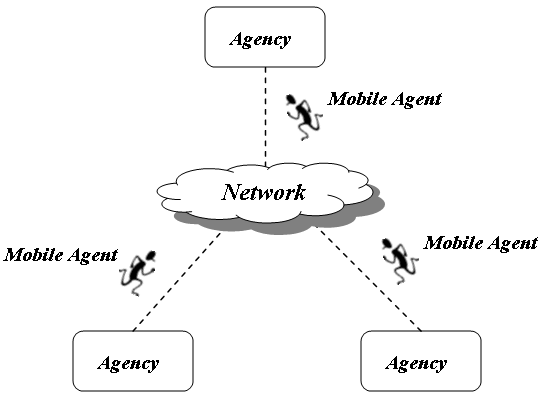
\includegraphics[scale=0.6]{figure/coverfigure}}
%\end{figure}
%%%%%%%%%%%%%%%%%%%% end figure %%%%%%%%%%%%%%%%%%%%%%
\end{abstract}
\pagebreak
% Abstract }}}
%%%%%%%%%%%%%%%%%%%%%%%%%%%%%%%%%%%%%%%%%%%%%%%%%%%%%%%%%%%%%%%%%%%%%%

%%%%%%%%%%%%%%%%%%%%%%%%%%%%%%%%%%%%%%%%%%%%%%%%%%%%%%%%%%%%%%%%%%%%%%
% Table of Contents {{{
\pagenumbering{roman}
\setcounter{page}{1}
\tableofcontents
\pagebreak
% }}} Table of Contents
%%%%%%%%%%%%%%%%%%%%%%%%%%%%%%%%%%%%%%%%%%%%%%%%%%%%%%%%%%%%%%%%%%%%%%

%%%%%%%%%%%%%%%%%%%%%%%%%%%%%%%%%%%%%%%%%%%%%%%%%%%%%%%%%%%%%%%%%%%%%%
% Part 1 {{{
\pagenumbering{arabic}
\setcounter{page}{1}
\pagebreak
% }}} Part 1 
%%%%%%%%%%%%%%%%%%%%%%%%%%%%%%%%%%%%%%%%%%%%%%%%%%%%%%%%%%%%%%%%%%%%%%

%%%%%%%%%%%%%%%%%%%%%%%%%%%%%%%%%%%%%%%%%%%%%%%%%%%%%%%%%%%%%%%%%%%%%%
% Introduction {{{
%\pagenumbering{arabic}
%\setcounter{page}{1}
%\pagestyle{fancy}
\chapter{Introduction}
Parallel and distributed computing~\cite{Kumar}~\cite{Manber} are widely used 
in scientific and engineering fields, especially for time-critical or 
time-consuming tasks.
Parallel computing is typically carried out in dedicated multiprocessors with
a central clock and shared memory.
On the other hand, distributed computing is decentralized parallel
computing, using two or more computers communicating over a network to
accomplish a common objective or task.
It is similar to computer clustering with the main difference being a wide
geographic dispersion of the resources.
In addition to the main difference, the types of hardware, programming 
languages, operating systems and other resources may vary drastically as well 
in distributed computing.

Although the processing speed of networked computers is typically not as fast 
as that of a dedicated parallel computer, networked computers are less
expensive and more broadly available.
Due to the rapid improvement in network hardware and software that makes
distributed computing faster, more broadly available, and easier-to-implement
than before, there are more and more research investigations nowadays 
targeting or exploiting this low-end, decentralized parallel computing.
Meanwhile, as the scale of distributed applications rapidly expands, 
there is an increasing demand for the code mobility.

Agent technology can significantly enhance the design and analysis of 
problem domains under the following three conditions~\cite{Adler}: 
(1) the problem domain is geographically distributed; 
(2) the subsystems exist in a dynamic environment; 
(3) the subsystems need to interact with each other more flexibly. 
Mobile agents are software components that can travel between 
different execution environments~\cite{Fuggetta}. 
Mobile agents can be created dynamically during runtime and dispatched to 
source systems to perform tasks with the most updated code. 
Therefore, the mobility of mobile agents provides distributed 
applications with significant flexibility and adaptability which are both 
essential to satisfy the dynamically changing requirements and conditions in 
a distributed environment.

Most of the mobile agent systems were developed to support only Java mobile 
agents.
Furthermore, many of them are standalone platforms. 
In other words, they were not designed to be embedded in a user application 
to support code mobility.  
Mobile-C~\cite{Chenthesis}~\cite{Chen3}~\cite{Mobile-C}~\cite{mobilec_webpage} 
was originally developed as a standalone, IEEE Foundation for Intelligent 
Physical Agents (FIPA) compliant mobile agent platform with a primary 
intention to fit applications where low-level hardware gets involved, such as 
networked mechatronic and embedded systems. 
Since most of these systems are written in C/C++, Mobile-C uses C/C++ as 
the mobile agent language for easy interfacing with control programs and 
underlying hardware. 
In addition, Mobile-C uses an embeddable C/C++ interpreter -- Ch, originally 
developed by Cheng~\cite{SP1}~\cite{CUJ1}~\cite{Ch}, to support the execution 
of C/C++ mobile agent code. 

In order to provide distributed applications with code mobility, this 
user's guide presents a mobile agent library, the Mobile-C library. 
The Mobile-C library is supported in various operating systems including 
Windows, Unix, and real-time OS.
It has a small footprint to satisfy the small memory requirement for a 
variety of mechatronic and embedded systems. 
This mobile agent library allows Mobile-C to be embedded in a program to 
support C/C++ mobile agents.
The API functions in this library facilitate the development of a multi-agent
system that can easily interface with a variety of hardware devices. 
%\pagebreak
% }}} Introduction
%%%%%%%%%%%%%%%%%%%%%%%%%%%%%%%%%%%%%%%%%%%%%%%%%%%%%%%%%%%%%%%%%%%%%%

%%%%%%%%%%%%%%%%%%%%%%%%%%%%%%%%%%%%%%%%%%%%%%%%%%%%%%%%%%%%%%%%%%%%%%
% Mobile-C Library Installation {{{
\chapter{Mobile-C Library Installation}
This chapter describes the prerequisites to install the Mobile-C library and 
the installation steps for both Unix and Windows operating systems.

%%%%%%%%%%%%%%%%%%%%%%%%%%%%%%%%%%%%%%%%%%%%%%%%%%%%%%%%%%%%%%%%%%%%%%
% SUB: Requirements {{{
\section{Requirements}
This user's guide assumes all necessary software packages are installed
correctly and function. 
The software packages required to successfully install the Mobile-C library 
include:

\noindent
(1) Ch version 6.3.0 or greater: It can be obtained from http://www.softintegration.com

\noindent
(2) Embedded Ch version 6.3.0 or greater: It can be obtained from http://www.softintegration.com

% }}} SUB: Prerequisites 
%%%%%%%%%%%%%%%%%%%%%%%%%%%%%%%%%%%%%%%%%%%%%%%%%%%%%%%%%%%%%%%%%%%%%%

%%%%%%%%%%%%%%%%%%%%%%%%%%%%%%%%%%%%%%%%%%%%%%%%%%%%%%%%%%%%%%%%%%%%%%
% SUB: Installation on Unix {{{
\section{Installation on Unix}

\subsection{Install the Mobile-C library}
The following commands will install the Mobile-C library in the system 
directory for {\bf 32-bit} Unix systems. 
The system directory for Unix systems is usually `/usr/local/lib' or 
  `/usr/lib' depending on your system.

\begin{verbatim}
    cd <MCPACKAGE>/src
    ./configure
    make
    make install
\end{verbatim}

The following commands will install the Mobile-C library in the system 
  directory for {\bf 64-bit} Unix systems. 
The only difference between the above and below commands is that `fPIC' is 
  added into CFLAGS for compilation.

\begin{verbatim}
    cd <MCPACKAGE>/src
    ./configure CFLAGS=-fPIC
    make
    make install
\end{verbatim}

By default, the Mobile-C library created contains both shared and static 
versions, which are `libmc.so.0.0.0' and `libmc.a', respectively.
The header file, libmc.h, used in the C/C++ binary 
space will be placed in the system directory, which is usually 
`usr/local/include' or `/usr/include' depending on your system.
 
Note that these commands will automatically build mxml-2.2.2 and
xyssl-0.7, both of which are packaged with Mobile-C, but will
not install these libraries. The Mobile-C libraries only need
these libraries to compile, but does not need them installed in
order to run.

Also note that the above commands will automatically compile all the included
demos automatically after compiling the Mobile-C library. The demos will
run even if the 'make install' step is omitted.

The `--prefix' option can be used to specify the home directory to 
install the Mobile-C files, as shown in the following commands.

\begin{verbatim}
    cd <MCPACKAGE>/src
    ./configure --prefix=<MCHOME>
    make
    make install
\end{verbatim}

\noindent
\texttt{<MCPACKAGE>} is the directory created by unpacking the Mobile-C compressed 
tar file.
\texttt{<MCHOME>} is the installation directory for the Mobile-C library and 
header file.\\
\noindent
The library files `libmc.so.0.0.0' and `libmc.a' will be installed in 
\texttt{<MCHOME>/lib}, and the header file `libmc.h' will be placed in 
\texttt{<MCHOME>/include}.

% }}} SUB: Installation on Unix
%%%%%%%%%%%%%%%%%%%%%%%%%%%%%%%%%%%%%%%%%%%%%%%%%%%%%%%%%%%%%%%%%%%%%%

%%%%%%%%%%%%%%%%%%%%%%%%%%%%%%%%%%%%%%%%%%%%%%%%%%%%%%%%%%%%%%%%%%%%%%
% SUB: Installation on Windows {{{
\section{Installation on Windows}
\subsection{Building the Mobile-C Library}
The following steps are suggested to build the Mobile-C library.
\begin{enumerate}
\item Ensure that your \texttt{\_chrc} file in your home directory is up to
  date. The \texttt{\_chrc} file may be opened from the ChIDE text editor by
  opening ChIDE, selecting "Options" from the menu, and selecting the "Open
  Local Ch Startup File" menu item. The section in your \texttt{\_chrc} file
  which contains settings about
  your Visual C++ installation must be correct. 
\item Unpack the Mobile-C source code. Ensure that you have write permissions
  for the directory you are unpacking Mobile-C into, or you may encounter 
  compile-time errors. As mentioned in the previous section, we will refer
  to the unpacked directory as \texttt{<MCPACKAGE>}.
\item Open a Ch terminal.
\item Navigate to the \texttt{<MCPACKAGE>} directory in your Ch terminal. For
  example, if you unpacked Mobile-C to the \texttt{C:$\backslash$Mobile-C} directory, type
  \texttt{cd C:$\backslash$Mobile-C} in your Ch terminal.
\item Type the command \texttt{nmake -f makefile.win32} to build the Mobile-C
  library, as well as all of the demos in the \texttt{<MCPACKAGE>/demos/}
  directory.
\end{enumerate}
% }}} SUB: Installation on Windows 
%%%%%%%%%%%%%%%%%%%%%%%%%%%%%%%%%%%%%%%%%%%%%%%%%%%%%%%%%%%%%%%%%%%%%%

%%%%%%%%%%%%%%%%%%%%%%%%%%%%%%%%%%%%%%%%%%%%%%%%%%%%%%%%%%%%%%%%%%%%%%
% SUB: Installation on KoreBot {{{
\section{Installation on KoreBot}

\subsection{Build the Mobile-C library}
A bash script, \textit{build\_korebot}, is used to build the Mobile-C library 
and an executable sample program, \textit{mc\_sample\_app}, for KoreBot board.

Running the script will create a directory called \textit{korebot\_mc} that 
contains \textit{bin}, \textit{include} and \textit{lib} directories.
\textit{bin} directory contains the executable sample program.    
\textit{include} directory contains the header file \textit{libmc.h}.
\textit{lib} directory contains the Mobile-C related static and shared 
libraries.

Two paths, \textit{KOREBOT\_CHHOME} and \textit{KOREBOT\_TOOLCHAINHOME}, 
in the bash script might need to be changed to match the correct 
paths set up in a user's system.
\textit{KOREBOT\_CHHOME} is the directory containing Ch files built for 
KoreBot board.
\textit{KOREBOT\_TOOLCHAINHOME} is the directory containing cross compiler 
related files for KoreBot board. 

Use the following commands to run the bash script.

\begin{verbatim}
    cd <MCPACKAGE>
    ./build_korebot
\end{verbatim}
% }}} SUB: Installation on KoreBot 
%%%%%%%%%%%%%%%%%%%%%%%%%%%%%%%%%%%%%%%%%%%%%%%%%%%%%%%%%%%%%%%%%%%%%%

%%%%%%%%%%%%%%%%%%%%%%%%%%%%%%%%%%%%%%%%%%%%%%%%%%%%%%%%%%%%%%%%%%%%%%
% SUB: Installation on Gumstix {{{
\section{Installation on Gumstix}

\subsection{Build the Mobile-C library}
A bash script, \textit{build\_gumstix}, is used to build the Mobile-C library 
and an executable sample program, \textit{mc\_sample\_app}, for Gumstix 
computer.

Running the script will create a directory called \textit{gumstix\_mc} that 
contains \textit{bin}, \textit{include} and \textit{lib} directories.
\textit{bin} directory contains the executable sample program.    
\textit{include} directory contains the header file \textit{libmc.h}.
\textit{lib} directory contains the Mobile-C related static and shared 
libraries.

Two paths, \textit{GUMSTIX\_CHHOME} and \textit{GUMSTIX\_TOOLCHAINHOME}, 
in the bash script might need to be changed to match the correct 
paths set up in a user's system.
\textit{GUMSTIX\_CHHOME} is the directory containing Ch files built for 
Gumstix computer. By default, it is set to the value \texttt{/usr/local/gumstix\_ch/ch/}.
\textit{GUMSTIX\_TOOLCHAINHOME} is the directory containing cross compiler 
related files for Gumstix computer. By default, it is set to the value \texttt{/usr/local/gumstix-buildroot}.

Use the following commands to run the bash script.

\begin{verbatim}
    cd <MCPACKAGE>
    ./build_gumstix
\end{verbatim}
% }}} SUB: Installation on Gumstix 
%%%%%%%%%%%%%%%%%%%%%%%%%%%%%%%%%%%%%%%%%%%%%%%%%%%%%%%%%%%%%%%%%%%%%%

%%%%%%%%%%%%%%%%%%%%%%%%%%%%%%%%%%%%%%%%%%%%%%%%%%%%%%%%%%%%%%%%%%%%%%
% Installing the Mobile-C Ch Package{{{
\section{Installing the Mobile-C Ch Package}
The Mobile-C Ch Package will be required if agents need to use any of the
Mobile-C FIPA ACL message functions, such as \texttt{mc\_AclSend()} or
\texttt{mc\_AclRetrieve()}. To install the Mobile-C Ch package, please follow
these steps:
\begin{enumerate}
\item From the Mobile-C root directory, run the command: \\
\texttt{ch ./pkgcreate.ch} \\
This will create a directory called ``\texttt{chmobilec}''.
\item From within a Ch shell, run the command: \\
\texttt{sudo pkginstall.ch chmobilec} \\
If you are using Microsoft Windows, you may omit the "\texttt{sudo}" part of the
command which is required on unix-like systems to ensure proper installation
permassions.
\end{enumerate}
% }}} Installing the Mobile-C Security Module
%%%%%%%%%%%%%%%%%%%%%%%%%%%%%%%%%%%%%%%%%%%%%%%%%%%%%%%%%%%%%%%%%%%%%%

\section{Creating your own compilation environment}
If a custom build environment is required, there are several directories which
must be added to the search paths for header files and libraries. There are 
also a variety of system libraries which Mobile-C must be linked with in order
to compile properly.

\subsection{UNIX and Mac systems}
In order to compile properly, the extra include directory
\texttt{<CHHOME>/extern/include} must be added to the default include search
directories. The directory \texttt{<CHHOME>/extern/lib} must also be added to
the list of searched library directories. Furthermore, the following libraries
must be linked with Mobile-C during the link step:
\begin{itemize}
\item libmxml (Provided with Mobile-C in the directory \texttt{<MCHOME>/src/mxml/})
\item libmc\_list (Provided with Mobile-C in the directory \texttt{<MCCHOME>/src/mc\_list})
\item libmc\_sync (Provided with Mobile-C in the directory \texttt{<MCCHOME>/src/mc\_sync})
\item libdl
\item libpthread
\item libm
\item libcrypt
\item libembedch (Provided with Embedded-Ch)
\end{itemize}

\subsection{Windows}
For windows, the include directory \texttt{<CHHOME>/extern/include} must be added
to the include paths and the directory \texttt{<CHHOME>/extern/lib} must be added
to the library search paths. Furthermore, the library \texttt{wsock32.lib} must
be linked with Mobile-C in order to compile properly.

% }}} Mobile-C Library Installation 
%%%%%%%%%%%%%%%%%%%%%%%%%%%%%%%%%%%%%%%%%%%%%%%%%%%%%%%%%%%%%%%%%%%%%%

%%%%%%%%%%%%%%%%%%%%%%%%%%%%%%%%%%%%%%%%%%%%%%%%%%%%%%%%%%%%%%%%%%%%%%
% Getting Started{{{
\chapter{Getting Started}
%%%%%%%%%%%%%%%%%%%%%%%%%%%%%%%%%%%%%%%%%%%%%%%%%%%%%%%%%%%%%%%%%%%%%%
% SUB: Compilation on Unix{{{
\section{Compilation on Unix}
All the demo programs are compiled automatically in the Unix version.
% }}} Compilation on Unix
%%%%%%%%%%%%%%%%%%%%%%%%%%%%%%%%%%%%%%%%%%%%%%%%%%%%%%%%%%%%%%%%%%%%%%

%%%%%%%%%%%%%%%%%%%%%%%%%%%%%%%%%%%%%%%%%%%%%%%%%%%%%%%%%%%%%%%%%%%%%%
% SUB: Compilation on Windows{{{
\section{Compilation on Windows}
All the demo programs are compiled automatically in the Windows version. Single
demos may be recompiled by navigating to a demo directory in a Ch terminal with
the \texttt{cd} and \texttt{ls} commands, and then executing the commands
\texttt{nmake -f makefile.win32} to compile a demo, or \texttt{nmake -f
makefile.win32 clean} to delete all compiled files.
% }}} SUB: Compilation on Windows 
%%%%%%%%%%%%%%%%%%%%%%%%%%%%%%%%%%%%%%%%%%%%%%%%%%%%%%%%%%%%%%%%%%%%%%

%%%%%%%%%%%%%%%%%%%%%%%%%%%%%%%%%%%%%%%%%%%%%%%%%%%%%%%%%%%%%%%%%%%%%%
% SUB: Overview of Sample Application Programs {{{
\section{Overview of Sample Application Programs}
%%%%%%%%%%%%%%%%%%%%%%%%%%%%%%%%%%%%%%%%%%%%%%%%%%%%%%%%%%%%%%%%%%%%%%
% Program: server.c {{{
\begin{Program}[!h]
\capstart
\begin{center}
   {\footnotesize \linespread{1.0} \verbatiminput{../demos/getting_started/hello_world/server.c}}
\end{center}
\caption{A sample Mobile-C server. (demos/getting\_started/hello\_world/server.c)}
\label{prog:server.c}
\end{Program}
% }}} Program: server.c
%%%%%%%%%%%%%%%%%%%%%%%%%%%%%%%%%%%%%%%%%%%%%%%%%%%%%%%%%%%%%%%%%%%%%%

%%%%%%%%%%%%%%%%%%%%%%%%%%%%%%%%%%%%%%%%%%%%%%%%%%%%%%%%%%%%%%%%%%%%%%
% Program: client.c {{{
\begin{Program}%[!h]
\capstart
\begin{center}
   {\footnotesize \linespread{1.0} \verbatiminput{../demos/getting_started/hello_world/client.c}}
\end{center}
\caption{A sample Mobile-C client program. The sole purpose of this program is to
  send a Mobile-C agent to another agency. (demos/getting\_started/hello\_world/client.c)}
\label{prog:client.c}
\end{Program}
% }}} Program: client.c
%%%%%%%%%%%%%%%%%%%%%%%%%%%%%%%%%%%%%%%%%%%%%%%%%%%%%%%%%%%%%%%%%%%%%%


Program \vref{prog:server.c} starts an agency that is capable of 
receiving mobile agents and executing mobile agent code. 

{\footnotesize \linespread{1.0} \verbatiminput{../demos/getting_started/hello_world/server.c.1}}
\noindent
The header file {\bf libmc.h} is included at the beginning of the program. 
It defines all the data types, macros and function prototypes for the 
Mobile-C library.

{\footnotesize \linespread{1.0} \verbatiminput{../demos/getting_started/hello_world/server.c.2}}
\noindent
The variable $agency$, of type {\bf MCAgency\_t}, is a handle that contains 
information of an agency. The second line initializes a local variable that will
hold the port number we wish the agency to bind to.

{\footnotesize \linespread{1.0} \verbatiminput{../demos/getting_started/hello_world/server.c.3}}
\noindent
{\bf MC\_Initialize()} \index{MC\_Initialize()} takes an integer and the address of an 
{\bf MCAgencyOptions\_t} \index{MCAgencyOptions\_t} variable as its two parameters. 
An {\bf MCAgencyOptions\_t} variable is a structure that contains 
information about which threads to be activated and the default agent 
status specified by a user.
Here, a {\bf NULL} pointer is passed to {\bf MC\_Initialize()} as the second 
parameter instead of an MCAgencyOptions\_t variable to start an agency with 
default settings. 
A local agency will be initialized to listen on port {\bf 5051} specified by 
the variable $local\_port$.

{\footnotesize \linespread{1.0} \verbatiminput{../demos/getting_started/hello_world/server.c.4}}
\noindent
The agency waits indefinitely for a mobile agent by the function 
{\bf MC\_MainLoop()} \index{MC\_MainLoop()}. 

Program \ref{prog:client.c} starts an agency that sends a mobile agent to 
a remote agency.
Examining Programs \ref{prog:server.c} and \ref{prog:client.c}, we see
that there are only two new API function calls:
\begin{verbatim}
  agent = MC_ComposeAgentFromFile(
      "mobagent1",      /* Name */
      "localhost:5050", /* Home */
      "IEL",            /* Owner */
      "hello_world.c",  /* Filename */
      NULL,             /* Return var name. NULL for no return */
      "localhost:5051", /* Server to execute task on */
      0 );              /* Persistent. 0 for no persistence. */
\end{verbatim}
and
\begin{verbatim}
  MC_AddAgent(agency, agent);
\end{verbatim}

Mobile-C agents may be created from existing source code files. The example
above takes a source code file called \texttt{hello\_world.c} and constructs
an agent around it. The agent's name, home, owner, return variable name,
and the host on which to execute the agent are all provided as arguments
to the \texttt{MC\_ComposeAgentFromFile()} function. 

Then, the newly created agent is added to the local agency so that it may
perform its local and/or remote tasks. In our example, the agent has
one remote task, so the agent will migrate to the remote host and perform
its task there. 

Also note that any valid hostname may be used in place of ``localhost''. The
communicating agencies need not be on the same physical machine; in fact, in most
cases they will be on seperate machines. Any IPv4 string, i.e. ``169.237.104.199'', or
qualified hostname, i.e. ``machine.ucdavis.edu'', may be used. For instance, the
code
\begin{verbatim}
    MC_ComposeAgentFromFile(
                "Bob",
                "iel.ucdavis.edu:5050",
                "IEL",
                "source_code.c",
                "169.237.104.199:5055",
                NULL,
                0);
\end{verbatim}
will send an agent to the server at address ``169.237.104.199'' listening on
port 5055. Or,
\begin{verbatim}
    MC_ComposeAgentFromFile(
                "Lou",
                "iel.ucdavis.edu:5055",
                "IEL",
                "agent_source.c",
                "machine.ucdavis.edu:5031",
                NULL,
                0);
\end{verbatim}
will send the agent to an agency at ``machine.ucdavis.edu'' listening on 
port 5031.
% }}} SUB: Overview of Sample Application Programs
%%%%%%%%%%%%%%%%%%%%%%%%%%%%%%%%%%%%%%%%%%%%%%%%%%%%%%%%%%%%%%%%%%%%%%

%%%%%%%%%%%%%%%%%%%%%%%%%%%%%%%%%%%%%%%%%%%%%%%%%%%%%%%%%%%%%%%%%%%%%%
% SUB: Mobile-C Bluetooth Agencies {{{
\section{Mobile-C Bluetooth Agencies (Experimental)}
As of Mobile-C version 2.0.2, Mobile-C has support for using Bluetooth
as the agent message transport medium as opposed to the standard TCP/IP.
A new option has been added to the \texttt{MCAgencyOptions\_t} structure
to indicate whether or not Mobile-C should start as a Bluetooth enabled
agency.

Please note that currently, Mobile-C is unable to start as both a Bluetooth
agency and a standard TCP/IP agency. That is, if a Mobile-C agency is
initialized to communicate via Bluetooth, that same agency will not be able to
communicate via TCP/IP, and vise versa. 

When Mobile-C is initialized as a Bluetooth agency, it enables Mobile-C to
send and receive messages to other Mobile-C Bluetooth agencies, via the
short/medium range Bluetooth wireless protocol. A sample Mobile-C 
server program that listens for incoming connections is shown below.

{\footnotesize \linespread{1.0} \verbatiminput{../demos/getting_started/bluetooth/server.c}}

Note that this program is very similar to the previous ``hello world''
server.c, seen at Program \ref{prog:server.c}. One major difference to take
note is the line which reads

\begin{verbatim}
options.bluetooth = 1;
\end{verbatim}

This line sets the option in the Mobile-C options structure to inform Mobile-C
to initialize as a Bluetooth agency.

Also note the initializing port number. Bluetooth RFCOMM port numbers are
limited to values from 0 to 30. The value  ``20'' was chosen arbitrarily, but
it must lie between zero and thirty. 

The client program, which sends an agent to the server agency, is also similar
to the previous client program seen at Program \ref{prog:client.c}.

{\footnotesize \linespread{1.0} \verbatiminput{../demos/getting_started/bluetooth/client.c}}

Note that the hostname supplied to the \texttt{MC\_ComposeAgentFromFile()}
function is composed of the MAC address of the server Bluetooth device,
followed by a space, followed by the port the server agency is listening on.

% }}} SUB: Mobile-C Bluetooth Agencies
%%%%%%%%%%%%%%%%%%%%%%%%%%%%%%%%%%%%%%%%%%%%%%%%%%%%%%%%%%%%%%%%%%%%%%

%%%%%%%%%%%%%%%%%%%%%%%%%%%%%%%%%%%%%%%%%%%%%%%%%%%%%%%%%%%%%%%%%%%%%%
% SUB: Execution of Sample Applications {{{
\section{Execution of Sample Applications}
In general, each of the demos is designed to have very similar execution
procedures. For each demo, there are one or more ``servers'', which are
simply vanilla Mobile-C agencies. To run the demo, start all of the servers
(there is only one server for most of the demos), and start the ``client''
program. Generally, the client program also starts a Mobile-C agency,
but it typically sends an agent to a destination as part of its startup
process as well.

For example, to run the Mobile-C ``Hello World'' example, 
run the following commands from a text terminal on the server machine
to start an agency listening on port {\bf 5051}.

\begin{verbatim}
    cd <MCPACKAGE>/demos/hello_world
    ./server
\end{verbatim}

\noindent
Next, run the following commands from a text terminal on the client machine
to start an agency listening on 
port {\bf 5050} and send the mobile agent to the remote agency 
listening on port {\bf 5051}.\\

\begin{verbatim}
    cd <MCPACKAGE>/demos/hello_world
    ./client
\end{verbatim}

\noindent
After the mobile agent message is received and the mobile agent code is 
executed, the string {\bf Hello World!} should be printed to the text terminal 
on the server machine. Note that in this example, both the server and client
are running on the same machine, but this is not a requirement. The field
``localhost'' may be replaced with any qualified domain name or IP address. 


% }}} Execution of Sample Applications
%%%%%%%%%%%%%%%%%%%%%%%%%%%%%%%%%%%%%%%%%%%%%%%%%%%%%%%%%%%%%%%%%%%%%%

%%%%%%%%%%%%%%%%%%%%%%%%%%%%%%%%%%%%%%%%%%%%%%%%%%%%%%%%%%%%%%%%%%%%%%
% The Mobile-C Library {{{
\section{The Mobile-C Library}
The Mobile-C library allows a Mobile-C agency to be embedded in a program to 
support C/C++ mobile agents.
In addition, the Mobile-C API gives users a full control over a Mobile-C 
agency embedded in a program. 
Therefore, the Mobile-C library not only provides a significant code mobility 
for distributed applications, but also facilitates the development of a 
multi-agent system that can easily interface with various hardware devices. 

%%%%%%%%%%%%%%%%%%%%%%%%%%%%%%%%%%%%%%%%%%%%%%%%%%%%%%%%%%%%%%%%%%%%%%
% FIGURE {{{ 
\begin{figure*}[!t]
\begin{center}
   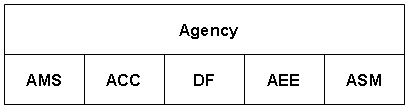
\includegraphics[scale=0.5]{figure/mobilec_lib_arch}
   \caption{Architecture of the Mobile-C library.}
   \label{fig:mobilec_lib_arch}
\end{center}
\end{figure*}
% FIGURE }}} 
%%%%%%%%%%%%%%%%%%%%%%%%%%%%%%%%%%%%%%%%%%%%%%%%%%%%%%%%%%%%%%%%%%%%%%

%%%%%%%%%%%%%%%%%%%%%%%%%%%%%%%%%%%%%%%%%%%%%%%%%%%%%%%%%%%%%%%%%%%%%%
% FIGURE {{{ 
\begin{figure*}[!t]
\begin{center}
   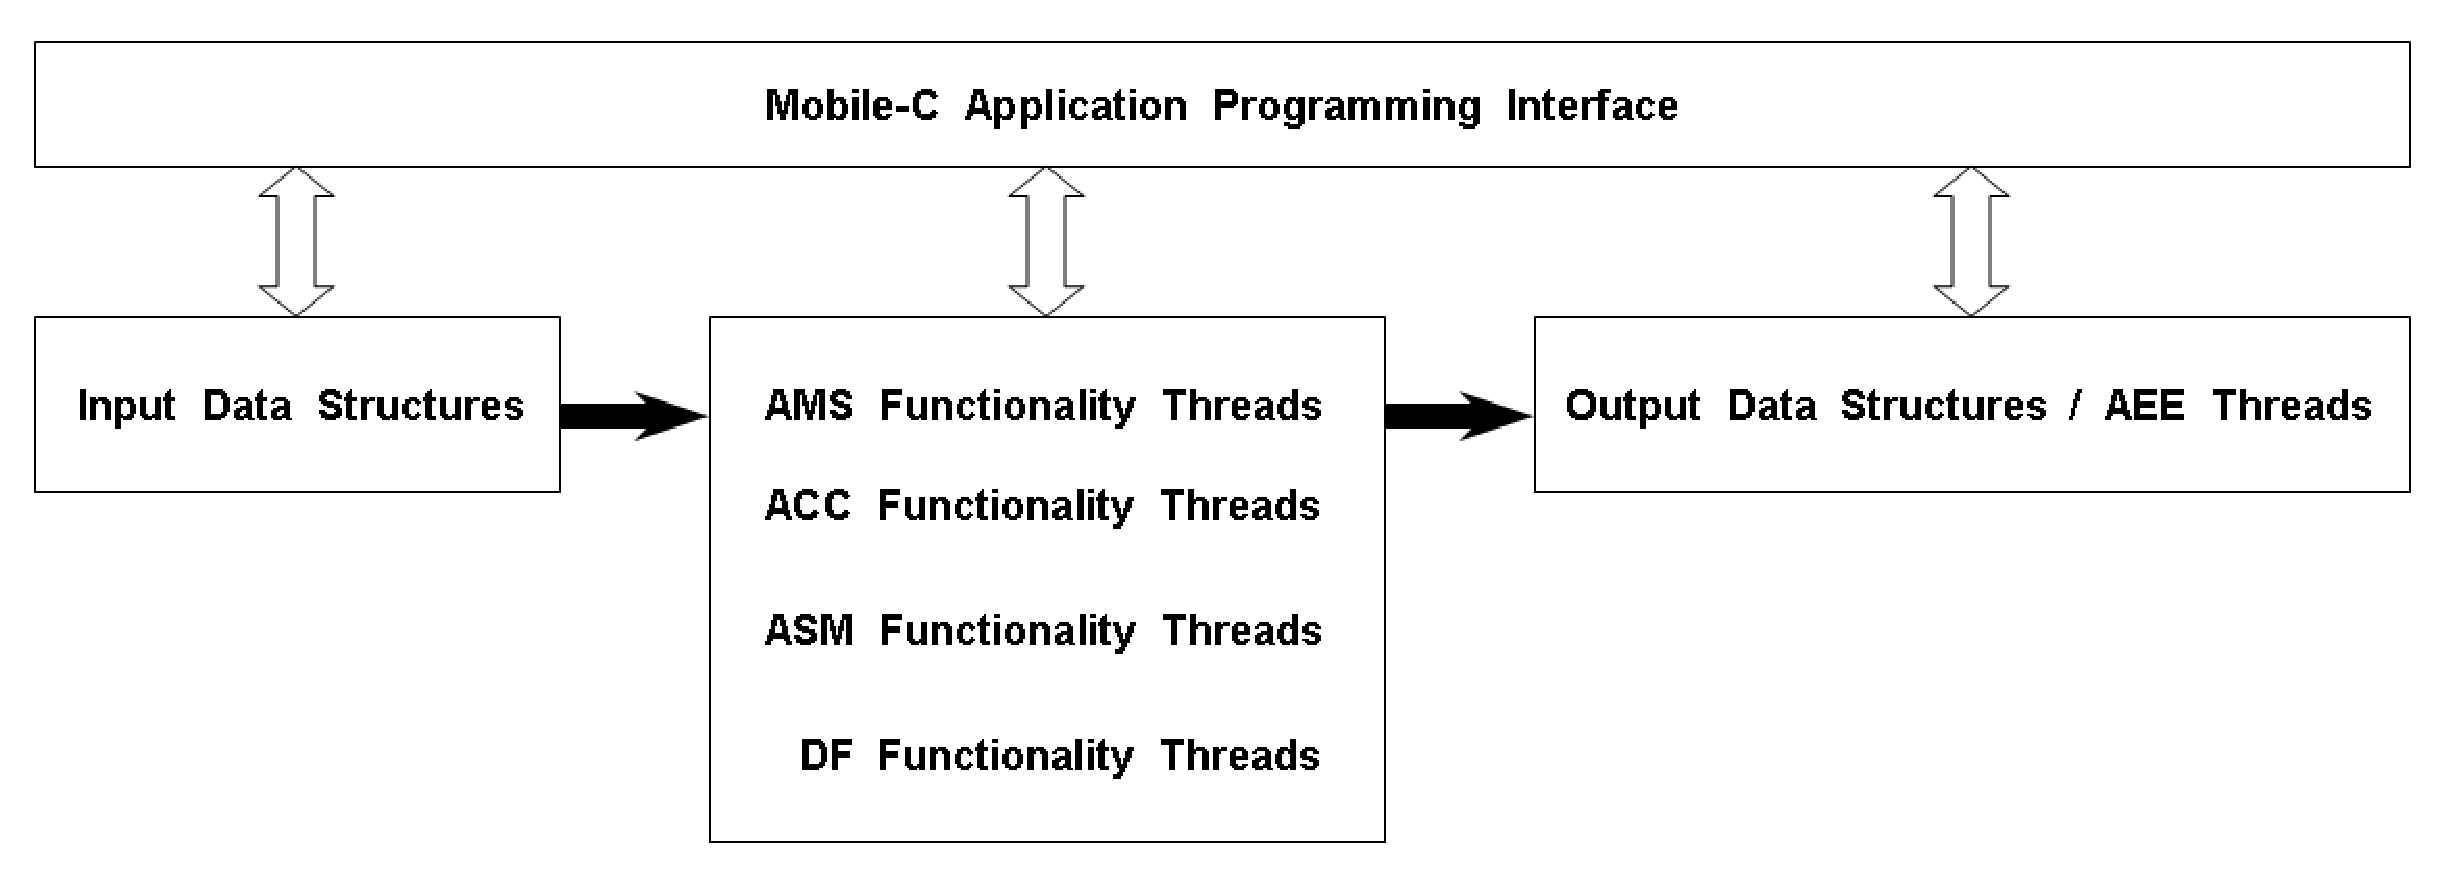
\includegraphics[scale=0.5]{figure/mobilec_lib_imp}
   \caption{Implementation overview of the Mobile-C library.}
   \label{fig:mobilec_lib_imp}
\end{center}
\end{figure*}
% FIGURE }}} 
%%%%%%%%%%%%%%%%%%%%%%%%%%%%%%%%%%%%%%%%%%%%%%%%%%%%%%%%%%%%%%%%%%%%%%

%%%%%%%%%%%%%%%%%%%%%%%%%%%%%%%%%%%%%%%%%%%%%%%%%%%%%%%%%%%%%%%%%%%%%%
% Architecture of the Mobile-C Library {{{
\subsection{Architecture of the Mobile-C Library \label{mobilec_arch}}
Figure \ref{fig:mobilec_lib_arch} illustrates the architecture of the 
Mobile-C library.
The Mobile-C library allows a Mobile-C agency to be embedded in a program to 
support C/C++ mobile agents.
A Mobile-C agency refers to a mobile agent platform within which mobile agents 
exist and operate.
The Mobile-C API gives users a full control over a Mobile-C agency and its 
different modules.
 
As a IEEE FIPA compliant mobile agent platform, a Mobile-C agency 
comprises three FIPA normative modules, Agent Management System (AMS), 
Agent Communication Channel (ACC) and Directory Facilitator (DF). 
Two additional modules, Agent Execution Engine (AEE) and 
Agent Security Manager (ASM), are included in a Mobile-C agency as well.
These modules provide different functionalities summarized as follows.

\textit{Agent Management System (AMS)}

\noindent
An AMS controls the creation, registration, execution, migration, 
persistence, and termination of a mobile agent. 
It maintains a directory of Agent Identifiers (AIDs) for registered mobile 
agents. 
Each mobile agent must register with an AMS in order to have a valid AID.

\textit{Agent Communication Channel (ACC)}

\noindent
An ACC routes messages between local and remote entities. 
It is responsible for the interactions between distributed components, such 
as inter-agent communication and inter-platform agent transport. 
The interactions can be performed through Agent Communication Language (ACL) 
message exchange.

\textit{Directory Facilitator (DF)}

\noindent
A DF serves yellow page services. 
Mobile agents wishing to advertise their services should register with a DF. 
Visiting mobile agents can search a DF for mobile agents providing the 
services they desire.

\textit{Agent Execution Engine (AEE)}

\noindent
An AEE serves as the execution environment for mobile agent code.
An AEE has to be platform independent in order to support the execution of 
mobile agents in a heterogeneous environment. 

Each AEE contains an Embedded Ch interpreter to interpret the agent C code.
By default, the agency will preload four interpreters upon startup for
interpreting agents. If more than four interpreters are required, the agency
will dynamically allocate extra interpreters as needed. See the reference for
\texttt{MC\_Initialize()} on page \pageref{api:MC_Initialize} for more info.

\textit{Agent Security Manager (ASM)}

\noindent
An ASM is responsible for maintaining securita policies for the host system.
Some sample tasks of an ASM include identifying users, protecting host 
resources, authenticating and authorizing mobile agents, and ensuring the 
security and integrity of mobile agents.
% }}} Architecture of the Mobile-C Library
%%%%%%%%%%%%%%%%%%%%%%%%%%%%%%%%%%%%%%%%%%%%%%%%%%%%%%%%%%%%%%%%%%%%%%

%%%%%%%%%%%%%%%%%%%%%%%%%%%%%%%%%%%%%%%%%%%%%%%%%%%%%%%%%%%%%%%%%%%%%%
% SUB: Implementation of the Mobile-C Library {{{
\subsection{Implementation of the Mobile-C Library}
Figure \ref{fig:mobilec_lib_imp} shows the implementation overview of the 
Mobile-C library.
The functionalities of each module of an agency are 
implemented as independent threads classified into five categories, that is, 
the AMS functionality threads, the ACC functionality threads, the DF 
functionality threads, the ASM functionality threads and the AEE threads.
Each AEE thread is launched by one of the AMS functionality threads.

The Mobile-C library provides API functions to specify which thread needs to 
be active or inactive when an agency is initialized.
It also provides API functions to access the input and output data structures 
associated with the functionality threads.
A Mobile-C agency maintains a list of synchronization variables that can be 
used with a group of Mobile-C functions to ensure synchronization among 
mobile agents and threads.
The sizes of the Mobile-C static and shared libraries for Linux are about 
500 KB and 390 KB, respectively.

The header file \textit{libmc.h} contains definitions of all the structures and 
functions of the Mobile-C library. 
Table \vref{mobilec_api_cbinary} lists the currently implemented functions 
for the binary space.

% }}} Implementation of the Mobile-C Library
%%%%%%%%%%%%%%%%%%%%%%%%%%%%%%%%%%%%%%%%%%%%%%%%%%%%%%%%%%%%%%%%%%%%%%

% }}} The Mobile-C Library
%%%%%%%%%%%%%%%%%%%%%%%%%%%%%%%%%%%%%%%%%%%%%%%%%%%%%%%%%%%%%%%%%%%%%%

% }}} Getting Started
%%%%%%%%%%%%%%%%%%%%%%%%%%%%%%%%%%%%%%%%%%%%%%%%%%%%%%%%%%%%%%%%%%%%%%

%%%%%%%%%%%%%%%%%%%%%%%%%%%%%%%%%%%%%%%%%%%%%%%%%%%%%%%%%%%%%%%%%%%%%%
% Composing Agents {{{
\chapter{Composing Agents}
Mobile-C agents are represented internally as XML data structures. However,
dealing with XML code requires background knowledge of XML and may be cumbersome.
To enhance the convenience of creating and deploying Mobile-C agents,
several different methods of creating agents from C source code files have
been implemented.

Agents may be composed from plain C source code. There are two main ways to
compose Mobile-C agents. Agents may be composed by using the
\texttt{compose\_send} commmand in the Mobile-C prompt, or by using the
\texttt{MC\_ComposeAgent*} series of API functions.

\section{Mobile-C Command Prompt \texttt{compose\_send} Command}
The \texttt{compose\_agent} takes a C source code file and creates
a fully functioning agent out of it. The \texttt{compose\_send} command
syntax is
\begin{verbatim}
compose_send <filename> <target host> <target port>
\end{verbatim}
Many details about an agent generated in this method, such as the agent's
name and owner, are dynamically generated when creating an agent using 
this method. 
\subsection{Example Execution Using the \texttt{compose\_send} Command}
The demo \texttt{prompt\_example} has been provided with the Mobile-C
package. Note that the source code for both servers is virtually identical to
that in Program \ref{prog:server.c}, except with added execution
instructions.
The demo program is initiated by starting the first agency, named
\texttt{server1}.
\begin{verbatim}
$ ./server1
Agency 1 started. Please start the second agency by running the command
"server2" on another terminal.

MobileC >
\end{verbatim}
Next, the second agency is started on a seperate terminal.
\begin{verbatim}
$ ./server2
Starting Agency...
You may now try the following commands:

  compose_send helloworld.c localhost 5050

The previous command will compose an agent using the source
code in "helloworld.c" and send it to the other agency at
port 5050. Then try this command:

  compose_send helloworld.c localhost 5051

This will send the "hello_world.c" agent to the local agency.
You may also try these commands at the other agency.

MobileC >
\end{verbatim}
Following the instructions on the second agency, we execute the 
suggested \texttt{compose\_send} command. The first agency terminal
now appears as such:
\begin{verbatim}
$ ./server1
Agency 1 started. Please start the second agency by running the command
  "server2" on another terminal.

MobileC > Hello, world!
\end{verbatim}
Note that the source file \texttt{helloworld.c} has been composed into a 
mobile agent, migrated to the \texttt{server1} agency, and executed.

\section{Mobile-C \texttt{MC\_ComposeAgent*} Functions}
There also exist a set of API functions which compose agents from C source
files. These functions are
\begin{itemize}
\item \texttt{MC\_ComposeAgent()} : Compose an agent from program source code. 
\item \texttt{MC\_ComposeAgentWithWorkgroup()} : Compose an agent from program source code with a workgroup code. 
\item \texttt{MC\_ComposeAgentFromFile()} : Compose an agent from a program source code file. 
\item \texttt{MC\_ComposeAgentFromFileWithWorkgroup()} : Compose an agent from a program source code file with a workgroup code. 
\item \texttt{MC\_AgentAddTask()} : Add an additional task to an already formed agent.
\item \texttt{MC\_AgentAddTaskFromFile()} : Add an additional task to an already formed agent from a C source code file.
\end{itemize}
For an example of the usage of these functions, please refer to program
\ref{prog:compose_multi_task_agent}.

\begin{Program}[p]
\begin{center}
   {\footnotesize \linespread{1.0}
     \verbatiminput{../demos/composing_agents/multi_task_example/client_abridged.c}}
\end{center}
\caption{An agency building an agent with multiple tasks from seperate source code files.}
\label{prog:compose_multi_task_agent}
\end{Program}

\section{Agent Workgroups}
In order to provide an added layer of organization and security, agents
may be created which belong to a workgroup. A workgroup's name may be an
ASCII text string of any length. If an agent belongs in a workgroup,
then certain actions on that agent may only be performed by other agents
in the same workgroup. Thus, if a group of agents keeps their workgroup
name private, no agents outside of that group will be able to terminate,
delete, or otherwise affect the agents within the workgroup. All agents are
still able to interact through FIPA ACL messages.

For an example of agent workgroups in action, please see the demo program
in the\\
 \texttt{demos/agent\_workgroup\_example} directory. 
% }}}
%%%%%%%%%%%%%%%%%%%%%%%%%%%%%%%%%%%%%%%%%%%%%%%%%%%%%%%%%%%%%%%%%%%%%%


%%%%%%%%%%%%%%%%%%%%%%%%%%%%%%%%%%%%%%%%%%%%%%%%%%%%%%%%%%%%%%%%%%%%%%
% Agent Data {{{
\chapter{Agent Data}
Agents have the ability to carry pieces of data with them as they migrate from
host to host. The data carried by an agent can be categorized into two broad
types: ``agent return data'' and ``agent saved variables''. 

\section{Agent Return Data}
  ``Agent return data'' is typically used to store a piece of data being
returned to the agent's home agency. For instance, if an agent is given a task
to obtain a single result from a remote host, the agent might store the result
as its agent return data. An agent may hold a single return value for each one
of its tasks. The return value may be of any standard C type, or an array of 
such a type. For instance, the \texttt{double} type, as well as
\texttt{double[5][3]} are both valid types for a piece of agent return data,
since both are examples of a standard C type or an array of a standard type.
User defined structs and unions may not be returned as a piece of return data.
 
In order to return a variable as agent return data, the name of the return variable
simply needs to be specified when composing the agent. No further API calls need to be
executed from within the agent code. Note that the return variable must be declared as
a global variable in the agent code.
For an example of an agent with multiple tasks returning information to its home agency,
please see Program \ref{prog:compose_multi_task_agent} on page
\pageref{prog:compose_multi_task_agent}.

\section{Agent Saved Variables} 
An ``agent saved variable'' is also carried with an agent as it migrates. However,
this type of variable is typically used for data that the agent itself has access
to as it completes its tasks. Furthermore, an agent may save the value of as many
variables as it desires per task. For instance, during an agent's first task, it
may save various values, like the number of other agents on the agency as an
\texttt{int}, and the name of the agency as a \texttt{char[80]}. After it
migrates to it's second task, it may access the variables it saved previously
on the first host. In this way, an agent could calculate the total number of
active agents in an agency network. In summary,

\begin{tabular}{l|cc}
 & Agent Return Data & Agent Saved Variable \\
\hline
May save multiple variables per task & & X \\
\hline
Data easily retrieved by home agency & X & X \\
\hline
Data saved to agent automatically  & & \\
without agent-space API calls & X & \\
\hline
Agent can access its own saved data & & X
\end{tabular}

\vspace{0.18in}
For example, consider an agent with the following tasks. The agent's first task
appears as such:
\verbatiminput{../demos/agent_migration_message_format/agent_saved_variables_example/task1.c}
Note that the variable to be saved must be a global variable. In the agent code, the agent
performs a call to the function \texttt{mc\_AgentVariableSave(mc\_current\_agent, "savevar");}
The first argument in the function is a handle to an agent. The handle \texttt{mc\_current\_agent} is
a special handle an agent has to itself. The second argument is a character string denoting the
name of the variable to save. In effect, this code saves the value of \texttt{savevar} to
itself. As shown in the preceding code, the \texttt{mc\_AgentVariableSave()} function may
be called multiple times on differing variable types and arrays. Each variable will be
saved to the agent prior to migration.

Here is an example of the agent's second task's code:
\verbatiminput{../demos/agent_migration_message_format/agent_saved_variables_example/task2.c}
Note the call to \texttt{mc\_AgentVariableRetrieve(mc\_current\_agent,
"savevar", 0);} in this code example. This function attempts to retrieve a
pointer to the saved variable. The first argument, as seen before, is a handle
to the agent itself. The second variable is the name of the variable to
retrieve. The third argument is the task from which to retrieve the variable,
with the value \texttt{0} being the first task. If the call succeeds, it will
return a valid pointer to the saved variable. If it fails, the function returns
\texttt{NULL}.



% Chapter: Agent Data }}}
%%%%%%%%%%%%%%%%%%%%%%%%%%%%%%%%%%%%%%%%%%%%%%%%%%%%%%%%%%%%%%%%%%%%%%


%%%%%%%%%%%%%%%%%%%%%%%%%%%%%%%%%%%%%%%%%%%%%%%%%%%%%%%%%%%%%%%%%%%%%%
% Mobile-C Agent Migration Message Format {{{
\chapter{Mobile-C Agent Migration Message Format}
\section{General Message Format \label{sec:gen_message_format}}
\begin{Program}
\begin{center}
   {\scriptsize \linespread{1.0} \verbatiminput{../demos/getting_started/hello_world/test1.xml}}
\end{center}
\caption{A rudimentary agent. (demos/getting\_started/hello\_world/test1.xml)}
\label{prog:hello_agent}
\end{Program}
The message format for an agent migration message is designed such that
multiple tasks and multiple code blocks can be migrated from agency to
agency. The message is an XML message with encapsulated C code. An example
of a rudimentary agent can be seen in Program \ref{prog:hello_agent} on 
page \pageref{prog:hello_agent}. 
Following is a brief description of each XML tag.
\begin{itemize}
\item \texttt{MESSAGE}: This tag indicates to Mobile-C that the following data
  is a Mobile-C message. The message type is included in the attribute
  ``message''.
\item \texttt{MOBILE\_AGENT}: This tag indicates that the contained data is a 
  Mobile-C agent.
\item \texttt{AGENT\_DATA}: This tag indicates that the contained data is data pertaining
  to this particular agent.
\item \texttt{NAME}: The name of the agent.
\item \texttt{OWNER}: The owner of the agent. 
\item \texttt{HOME}: The home of the agent. Any agent that has data to ``return'' will
	return it to this address by default.
\item \texttt{WG\_CODE}: The workgroup code of the agent. Workgroup codes are
kept secret by the agent. Only agents with matching workgroup codes are allowed
to perform certain operations on each other, such as agent deletion.
\item \texttt{TASKS}: This indicates that the following information pertains to the
  task or tasks the agent is intended to perform. Attributes found under the
  \texttt{TASKS} tag include:
  \begin{itemize}
    \item \texttt{task} : The total number of tasks the agent has.
    \item \texttt{num} : The task that the agent is currently on.
  \end{itemize}
\item \texttt{TASK}: Each seperate \texttt{TASK} tag indicates a seperate task for the agent
  to perform. The tasks may be seperate hosts and/or code blocks. In the
  rudimentary example, there is only one task. Listed below are the attributes of 
  \texttt{TASK} tags.
  \begin{itemize}
  \item \texttt{num}:           The number of the task. The first task is task number zero.
  \item \texttt{complete}:      Completeness of the task
  \item \texttt{server}:        The host to perform the task
  \item \texttt{return}:        Name of the return variable
  \item \texttt{persistent}:    Persistence of the agent
  \item \texttt{return\_value}: Return value, if not an array
  \item \texttt{code\_id}:      ID of the code block to execute
  \end{itemize}
\textit{complete} and \textit{server} are mandatory attributes, and others are 
optional attributes.  
\item AGENT\_CODE: Each AGENT\_CODE block represents a block of code that 
  the agent may execute. Agents with multiple code blocks may decide at run-time
  which block to execute. Valid attributes under the \texttt{AGENT\_CODE} tag
  include
  \begin{itemize}
    \item \texttt{id}: The id of the code segment, as referenced by the \texttt{TASK} 
      attribute, \texttt{code\_id}.
  \end{itemize}
\end{itemize}

\section{Multiple Tasks with a Single Code Block}
An agent may have an indefinite number of tasks. The agent will perform the tasks
in ther order that they are stated in the XML file, completing each one before
continuing to the next host. Following is an example of an agent which has
multiple tasks to perform, executing the same code block at each new host.
See Program \ref{prog:single_code_block} on page \pageref{prog:single_code_block} 
for an example.
\begin{Program}[p]
\begin{center}
   {\footnotesize \linespread{1.0} 
     \verbatiminput{../demos/composing_agents/multi_task_example/test_single_code_block1.xml}}
\end{center}
\caption{An example agent containing two tasks and a single code block.
  Note that variables ``mc\_host\_name'' and ``mc\_task\_progress'' are special built-in variables described in Table \vref{tab:agent_space_variables}.
  \index{mc\_host\_name}
  \index{mc\_task\_progress}
  \texttt{(<MCPACKAGE>/demos/composing\_agents/multi\_task\_example/test\_single\_code\_block.xml)} }
\label{prog:single_code_block}
\end{Program}
\addtocounter{Program}{-1}
\begin{Program}[p]
\begin{center}
   {\footnotesize \linespread{1.0} 
     \verbatiminput{../demos/composing_agents/multi_task_example/test_single_code_block2.xml}}
\end{center}
\caption{(Continued)}
\end{Program}

\section{Multiple Tasks with Multiple Code Blocks}
See Program \ref{prog:multi_code_block} on page \pageref{prog:multi_code_block}
for a more complicated example of agent code including multiple tasks and
  multiple code blocks. Note that each code block has an associated ID which is 
  refered to in the respective ``DATA'' tags. Also note that more than one ``DATA'' tag
  may refer to the same code block. Thus, an agent may have more ``DATA'' tags than
  code blocks.

\begin{Program}[p]
\begin{center}
   {\footnotesize \linespread{1.0} 
     \verbatiminput{../demos/composing_agents/multi_task_example/test_multi_code_block1.xml}}
\end{center}
\caption{An example agent containing two tasks and two code blocks. 
  \texttt{(<MCPACKAGE>/demos/composing\_agents/multi\_task\_example/test\_multi\_code\_block.xml)}} 
\label{prog:multi_code_block}
\end{Program}
\addtocounter{Program}{-1}
\begin{Program}[p]
\begin{center}
   {\footnotesize \linespread{1.0} 
     \verbatiminput{../demos/composing_agents/multi_task_example/test_multi_code_block2.xml}}
\end{center}
\caption{ (Continued) }
\end{Program}

\section {Multiple Mobile Agent performs Task on Multiple Hosts}
Program \ref{prog:multi_mobile_agent_client} on page \pageref{prog:multi_mobile_agent_client} is a client that sends two different mobile agents to two different hosts. In for loop, it waits for the arrival signal of mobile agent. When an agent arrives it prints the result and delete that agent. For loop is iterated same as total number of mobile agents send by client. The two mobile agents having different name are shown in Program \ref{prog:mobile_agent_1} and Program \ref{prog:mobile_agent_2}:  

\begin{Program}[p]
\begin{center}
   {\footnotesize \linespread{1.0}
     \verbatiminput{../demos/agent_migration_message_format/multi_data_retrieval/client.c}}
\end{center}
\caption{A client program that sends two mobile agents to two different hosts
  \texttt{(<MCPACKAGE>/demos/agent\_migration\_message\_format/multi\_data\_retrieval/client.c)}}
\label{prog:multi_mobile_agent_client}
\end{Program}

\begin{Program}[p]
\begin{center}
   {\footnotesize \linespread{1.0}
     \verbatiminput{../demos/agent_migration_message_format/multi_data_retrieval/test1.xml}}
\end{center}\caption{First mobile agent name "mobagent1" send by client (Program 6) to server 1   
  \texttt{(<MCPACKAGE>/demos/agent\_migration\_message\_format/multi\_data\_retrieval/test1.xml)}}
\label{prog:mobile_agent_1}
\end{Program}

\begin{Program}[p]
\begin{center}
   {\footnotesize \linespread{1.0}
     \verbatiminput{../demos/agent_migration_message_format/multi_data_retrieval/test2.xml}}
\end{center}\caption{Second mobile agent name "mobagent1" send by client (Program 6) to server 2
  \texttt{(<MCPACKAGE>/demos/agent\_migration\_message\_format/multi\_data\_retrieval/test2.xml)}}
\label{prog:mobile_agent_2}
\end{Program}

\section{Agent Return Messages}
If the ``\texttt{name}'' attribute in an agent's ``\texttt{DATA}'' tag
is not set to ``\texttt{no-return}'', the agent will generate an
agent-return message upon completion of all of its tasks. The agent will
generate a return message containing the contents of the variable name
specified in the ``\texttt{name}'' attribute. For instance, Program
\vref{prog:agent_with_return_data} shows a simple agent which 
will migrate to another agency, generate a three-dimensional array called
``\texttt{a}'', and return the contents of the array to the ``\texttt{HOME}''
host upon completion. Note that the return variable must be global
so that the contents are not destroyed upon completion of the \texttt{main}
function. 
  
  An example of the return message that is generated by
this agent can be seen in Program \vref{prog:return_agent}. Notice also in
the return message that the variable type has been changed from ``int'' as it
was in the original program to ``short'' and that the ``\texttt{dim}'' attribute
has been changed to $3$. This is because Mobile-C automatically
checks the type and dimension of the variable it is returning and assign
those attributes automatically.

\begin{Program}[p]
\begin{center}
   {\footnotesize \linespread{1.0} 
     \verbatiminput{../demos/agent_migration_message_format/mc_array_return_example/agent.xml}}
\end{center}
\caption{An agent which returns data upon completion of it's tasks.}
\label{prog:agent_with_return_data}
\end{Program}

\begin{Program}[p]
\begin{center}
   {\footnotesize \linespread{1.0} 
     \verbatiminput{../demos/agent_migration_message_format/mc_array_return_example/return_agent.xml}}
\end{center}
\caption{Agent return data xml format. Note: This XML code has been reformatted
  to a more human-readable format. The actual format generated may differ.}
\label{prog:return_agent}
\end{Program}

\section{Agent Saved Variables}
As of Mobile-C version 1.10.0, Mobile-C agents have the ability to save an 
arbitrary number of variables while migrating from task to task. Agents may
use the agent-space api functions \texttt{mc\_AgentVariableSave()} and
\texttt{mc\_AgentVariableRetrieve} to save and later retrieve variables.
An example agent which does this may be viewed at the documentation for
the \texttt{mc\_AgentVariableSave()} and \linebreak \texttt{mc\_AgentVariableRetrieve()}
functions on pages \pageref{apidoc:mc_AgentVariableSave} and 
\pageref{apidoc:mc_AgentVariableRetrieve}, respectively.

As the agent is migrating from host to host with saved data, the data is 
encapsulated in the agent's XML code. \texttt{<DATA>} tags are created as
children of each \texttt{<TASK>} tag to store data. See Program 
\ref{prog:migrating_agent} for an example of an agent that is migrating
with saved data. The valid attributes within a \texttt{<DATA>} tag are
\begin{itemize}
\item \texttt{name}: The name of the saved variable.
\item \texttt{dim}: The array dimension of the saved variable. 
\item \texttt{type}: The type of the variable.
\item \texttt{value}: (optional) If the variable has zero dimensions, the
  value is stored in this attribute. Otherwise, children \texttt{<ROW>} 
  tags must be created to store the array.
\end{itemize}

Each \texttt{<DATA>} tag may also have children \texttt{<ROW>} tags, if
the data is an array. The valid attributes of the \texttt{<ROW>} tags are
\begin{itemize}
\item \texttt{index}: The index of the row.
\end{itemize}
Note also that each \texttt{<ROW>} tag may contain additional \texttt{<ROW>}
children depending on the dimension of the array being stored.

The Mobile-C XML Data Type Definition (DTD), which defines the format of a
well-formed Mobile-C agent migration message, may be seen in Section
\ref{sec:xml_dtd} on page \pageref{sec:xml_dtd}.

\section{Stationary/Persistent Mobile Agents}
A Stationary agent may be achieved in Mobile-C simply by creating an agent which
never migrates. This is commonly achieved using a couple of different
techniques.
\subsection{An Agent with an Infinite Task}
An agent may be considered stationary if it's task never ends. For instance, if
the task of an agent is of the form:
\begin{verbatim}
while(1)
{
    cmd = wait_for_command();
    execute_command(cmd);
}
\end{verbatim}
Since the previous task never ends, the agent will never terminate and the agent
will remain stationary in it's agency. 

\subsection{The ``\texttt{persistent}'' Agent Flag}
The ``\texttt{persistent}'' flag as mentioned in Section
\ref{sec:gen_message_format} may be used to create a persistent agent. The
example described in Chapter \ref{chap:interface_binary_to_agent} uses such a
technique. This technique creates an agent which is not automatically flushed by the agency
after it completes it's task. Thus, the agent remains dormant and stationary in
the agency without external stimulus.

\subsubsection{Terminating Persistent Agents}
Persistent agents should be terminated when they are no longer needed to free
up resources. They may be terminated by using the API functions 
\texttt{MC\_DeleteAgent()} or \texttt{MC\_TerminateAgent()} functions from C-space,
or the functions \texttt{mc\_DeleteAgent()} or \texttt{MC\_TerminateAgent()} functions 
from agent-space. Since a persistent agent cannot terminate itself, it is up to either
the host agency or another agent to terminate the persistent agent.

\begin{Program}[ph]
\begin{center}
{\footnotesize \linespread{1.0}
\verbatiminput{../demos/agent_migration_message_format/agent_saved_variables_example/migrating_agent.xml.part1}}
\end{center}
\caption{\label{prog:migrating_agent} This XML format illustrates an agent which is currently
in the process of migrating with saved data. Note that the agent contains two tasks, and the
first task has been completed. This file is a snapshot of the agent as it is in transit from
task '0' to task '1'. Note the \texttt{<DATA>} tags which store the three variables
referenced by the \texttt{mc\_AgentSaveVariable()} function from within the code, storing
two integers and an integer array. Note that in general, any data type may be stored, including
multi-dimensional arrays.}
\end{Program}
\addtocounter{Program}{-1}
\begin{Program}[ph]
\begin{center}
{\footnotesize \linespread{1.0}
\verbatiminput{../demos/agent_migration_message_format/agent_saved_variables_example/migrating_agent.xml.part2}}
\end{center}
\caption{(Continued)}
\end{Program}


% }}} Mobile-C Agent Migration Message Format
%%%%%%%%%%%%%%%%%%%%%%%%%%%%%%%%%%%%%%%%%%%%%%%%%%%%%%%%%%%%%%%%%%%%%%

%%%%%%%%%%%%%%%%%%%%%%%%%%%%%%%%%%%%%%%%%%%%%%%%%%%%%%%%%%%%%%%%%%%%%%
% {{{ Mobile-C FIPA Compliant ACL Messages
\chapter{Mobile-C FIPA Compliant ACL Messages \label{chap:fipa}}
Mobile-C has the ability to send and receive FIPA compliant
agent communication language (ACL) messages. More information
about FIPA, the Foundation for Intellegent Physical Agents, may be
found at \texttt{http://www.fipa.org}. This functionality allows
Mobile-C agent to communicate with each other, as well as with 
agents from other agencies that are also FIPA compliant. Demos
of communication with JADE agents may be found in the directories
\texttt{<MCPACKAGE>/demos/jade\_to\_mc\_example} and \\
\texttt{<MCPACKAGE>/demos/mc\_to\_jade\_example}.

%{{{ Constructing and Sending an ACL Message
\section{Constructing and Sending an ACL Message}
The general process for constructing an ACL message involves
filling out required portions of an ACL message structure of type
\texttt{struct fipa\_acl\_message\_s} and passing the message to the
\texttt{MC\_AclSend()} function. A number of helper functions 
exist in order to simplify the process of allocating memory and setting
certain fields of the acl message. 
Some typical functions used to compose a new ACL message are the following:
\begin{itemize}
\item \texttt{MC\_AclSetPerformative}: Set the FIPA performative of the message. See Program
  \ref{prog:fipa_enum} for a complete listing of valid FIPA performative enumerations.
\item \texttt{MC\_AclSetSender}: Sets the 'sender' field of the message.
\item \texttt{MC\_AclAddReceiver}: Adds addresses to the 'receiver' field of the message.
\item \texttt{MC\_AclSetContent}: Sets the 'content' field of an ACL message.
\end{itemize}
A detailed example of sending and receiving messages will be presented in
Chapter \ref{chap:stationary_agent}.
%}}}

%{{{Receiving an ACL Message 
\section{Receiving an ACL Message}
Every agent residing on a Mobile-C agency has a mailbox allocated to it.
At any time, the agent may check the mailbox for new ACL messages, or an
agent may choose to wait on an empty mailbox until a new message arrives.
These two tasks are done by the functions \texttt{MC\_AclRetreive()} and
\texttt{MC\_AclWaitRetrieve()}, respectively. 
Another useful function which may be used with a received ACL message is the
\texttt{MC\_AclReply()} function. This function takes an ACL message as an
input argument and automatically forms an ACL reply message addressed to the
original sender. Note that the performative and new sender fields in the reply
message are not automatically initialized and will still need to be set by
the agent. A detailed example of an agent receiving and replying to a message
may be found in Chapter \ref{chap:stationary_agent}.

\begin{Program}[!t]
\begin{center}
   {\footnotesize \linespread{1.0} 
\begin{verbatim}
enum fipa_performative_e
{
  FIPA_ERROR=-1,
  FIPA_ZERO,
  FIPA_ACCEPT_PROPOSAL,
  FIPA_AGREE,
  FIPA_CANCEL,
  FIPA_CALL_FOR_PROPOSAL,
  FIPA_CONFIRM,
  FIPA_DISCONFIRM,
  FIPA_FAILURE,
  FIPA_INFORM,
  FIPA_INFORM_IF,
  FIPA_INFORM_REF,
  FIPA_NOT_UNDERSTOOD,
  FIPA_PROPOGATE,
  FIPA_PROPOSE,
  FIPA_PROXY,
  FIPA_QUERY_IF,
  FIPA_QUERY_REF,
  FIPA_REFUSE,
  FIPA_REJECT_PROPOSAL,
  FIPA_REQUEST,
  FIPA_REQUEST_WHEN,
  FIPA_REQUEST_WHENEVER,
  FIPA_SUBSCRIBE
};
\end{verbatim}
   }
\end{center}
\caption{Fipa Performative Enumerations.}
\label{prog:fipa_enum}
\end{Program}

\pagebreak
\clearpage
\pagebreak
%}}} Section: Receiving an ACL Message

%}}} Chapter: Mobile-C FIPA Compliant ACL Messages
%%%%%%%%%%%%%%%%%%%%%%%%%%%%%%%%%%%%%%%%%%%%%%%%%%%%%%%%%%%%%%%%%%%%%%

%%%%%%%%%%%%%%%%%%%%%%%%%%%%%%%%%%%%%%%%%%%%%%%%%%%%%%%%%%%%%%%%%%%%%%
% Mobile-C Binary Stationary Agents {{{
\chapter{Mobile-C Binary Stationary Agents \label{chap:stationary_agent}}
Mobilec has support for hosting binary-space stationary agents. The
agents are implemented as system threads. As such, the only limit 
to the number of stationary agents residing on an agency are the
system resources of the host agency. 

The binary agents are able to call any of the C-space API functions, such as
\texttt{MC\_AclWaitRetrieve()}. This allows stationary agents to communicate
and interact with other mobile and stationary agents using FIPA ACL messages,
as introduced in Chapter \ref{chap:fipa}.

Stationary agents may be used in any application in which agent mobility is
unnecessary. Stationary agents can typically perform any task a mobile agent
can perform, except migration. Furthermore, stationary agents tend to execute
faster and consume less system resources.

Mobile-C stationary agent threads are added using the
\texttt{MC\_AddStationaryAgent()} API function. See Program 
\ref{prog:stationary_agent_server} for an example of a stationary agent. 

\begin{Program}[!t]
\begin{center}
   {\footnotesize \linespread{1.0} \verbatiminput{../demos/binary_stationary_agents/stationary_agent_communication/server.c}}
\end{center}
\caption{A sample program which starts a single stationary agent that responds to FIPA ACL messages.}
\label{prog:stationary_agent_server}
\end{Program}

The \texttt{MC\_AddStationaryAgent()} function takes three arguments:
\begin{enumerate}
\item A handle to the home agency. This is the agency the new agent will reside under.
\item The agent thread. This is a pointer to a function which will execute and act as
the stationary agent. If the function returns, the stationary agent is terminated.
\item An optional argument to pass to the agent. If additional information or data needs
to be passed to the stationary agent thread, a pointer of any type may be supplied as the
third argument to \\
\texttt{MC\_AddStationaryAgent()}. This pointer may later be retrieved
with the \\
\texttt{MC\_AgentInfo\_GetAgentArgs()} function from within the agent.
\end{enumerate}

The stationary agent thread must have a prototype of the form
\begin{verbatim}
void* agent_func_name(stationary_agent_info_t* agent_info);
\end{verbatim}
As seen in the prototype, the agent thread receives an argument of type
\texttt{stationary\_agent\_info\_t}. This special type is a structure 
which contains information about the the agent, such as its name, and the
location of its mailbox. Certain information may be retrieved from the 
function parameter by using the \texttt{MC\_AgentInfo\_*} series of API
functions, which include:
\begin{itemize}
\item \texttt{MC\_AgentInfo\_GetAgency()} : Retrieves a handle to the host agency.
\item \texttt{MC\_AgentInfo\_GetAgent()} : Retrieves a handle to the agent
information structure.
\item \texttt{MC\_AgentInfo\_GetAgentArgs()} : Retrieves the pointer that was
given as an agent argument during the call to \texttt{MC\_AddStationaryAgent}.
\end{itemize}

Example usage of these functions may be seen in Program \ref{prog:stationary_agent_server}.
%}}}
%%%%%%%%%%%%%%%%%%%%%%%%%%%%%%%%%%%%%%%%%%%%%%%%%%%%%%%%%%%%%%%%%%%%%%

%%%%%%%%%%%%%%%%%%%%%%%%%%%%%%%%%%%%%%%%%%%%%%%%%%%%%%%%%%%%%%%%%%%%%%
% Interface between Binary and Mobile Agent Spaces {{{
\chapter{Interface between Binary and Mobile Agent Spaces
\label{chap:interface_binary_to_agent}}
An embeddable C/C++ interpreter Ch was chosen to be the AEE in the Mobile-C 
library to support C/C++ mobile agents. 
Therefore, in order to access the variables, functions, and data sets in 
the mobile agent space from the binary space, Ch must be first embedded in the 
binary space.
The function \textit{MC\_GetAgentExecEngine()} \index{MC\_GetAgentExecEngine()} in 
Table \ref{mobilec_api_cbinary} returns the AEE associated with a mobile agent 
to the binary space.
Using the AEE returned by \textit{MC\_GetAgentExecEngine()}, all of the 
Embedded Ch functions~\cite{EmbeddedCh} can be called in a binary C/C++ 
program to access the variables, functions, and data sets defined in the 
mobile agent space.
The Embedded Ch toolkit also allows mobile agent code to invoke C/C++ 
functions defined in a binary C/C++ program.

The Embedded Ch toolkit reduces the complexity of heterogeneous development 
environment for both embedded scripting and applications. 
With the consistent C/C++ code base, it can significantly reduce the effort 
in the software development and maintenance. 
Moreover, with the Embedded Ch toolkit, C/C++ applications can be extended 
with all the features of Ch including built-in string type for scripting. 
The Embedded Ch toolkit has a small footprint. 
The pointer and time deterministic nature of the C language provide a 
perfect interface with hardware in real-time systems.

\section{Using an Agent Initialization Callback Function to Intergrate Binary
and Script Space Code}
The user may register a callback function to be called during the initialization
of mobile agents inside of an agency. This allows the user to fine-tune 
an agent and the Ch interpreter before an agent is executed. The callback
function is added using the \texttt{MC\_AddAgentInitCallback()} function,
and the callback function is of the form
\begin{verbatim}
int callback(ChInterp_t interp, MCAgent_t agent, void* user_data);
\end{verbatim}
The user may call any applicable Ch API function on the interpreter,
as well as any applicable Mobile-C API function on the supplied agent.
For instance, the user may use the \texttt{Ch\_DeclareVar()} function
to declare extra variables inside of the interpereter which the agent
will be able to access during its execution. 

The demo located at \texttt{demos/cspace-agentspace\_interface/agent\_init\_callback/} 
provides a demonstration of the callback function. This demo uses the callback
function to declare a new function in each of the incoming agent interpreters
called \texttt{mult()}, which simply multiplies two numbers together. This
means that any incoming agent will be able to call the \texttt{mult()} function,
which resides in C-space, from the agent script-space. This demo may also be seen with
the documentation for \texttt{MC\_AddAgentInitCallback()} on page \pageref{api:MC_AddAgentInitCallback()}.

%%%%%%%%%%%%%%%%%%%%%%%%%%%%%%%%%%%%%%%%%%%%%%%%%%%%%%%%%%%%%%%%%%%%%%
% Invoke a Mobile Agent Space Function from Binary Space {{{
\noindent
\section{Invoke a Mobile Agent Space Function from Binary Space}
%%%%%%%%%%%%%%%%%%%%%%%%%%%%%%%%%%%%%%%%%%%%%%%%%%%%%%%%%%%%%%%%%%%%%%
% client.c {{{
\begin{Program}[!t]
\begin{center}
   {\footnotesize \linespread{1.0} 
     \verbatiminput{../demos/cspace-agentspace_interface/persistent_example/client.c}}
\end{center}
\caption{ A program which sends a persistent mobile agent.
  \texttt{(<MCPACKAGE>/demos/cspace-agentspace\_interface/persistent\_example/client.c)}}
\label{prog:client_ex2.c}
\end{Program}
% }}} client.c
%%%%%%%%%%%%%%%%%%%%%%%%%%%%%%%%%%%%%%%%%%%%%%%%%%%%%%%%%%%%%%%%%%%%%%
%%%%%%%%%%%%%%%%%%%%%%%%%%%%%%%%%%%%%%%%%%%%%%%%%%%%%%%%%%%%%%%%%%%%%%
% test1.xml {{{
\begin{Program}[!t]
\begin{center}
   {\footnotesize \linespread{1.0} 
     \verbatiminput{../demos/cspace-agentspace_interface/persistent_example/test1.xml}}
\end{center}
\caption{A persistent mobile agent. Agents marked ``persistent'' are
  not flushed from the agency after they terminate.
    \texttt{(<MCPACKAGE>/demos/cspace-agentspace\_interface/persistent\_example/test1.xml)}}
\label{prog:mobileagent_ex2.xml}
\end{Program}
% }}} test2.xml
%%%%%%%%%%%%%%%%%%%%%%%%%%%%%%%%%%%%%%%%%%%%%%%%%%%%%%%%%%%%%%%%%%%%%%
%%%%%%%%%%%%%%%%%%%%%%%%%%%%%%%%%%%%%%%%%%%%%%%%%%%%%%%%%%%%%%%%%%%%%%
% host.c {{{
\begin{Program}[!t]
\begin{center}
   {\footnotesize \linespread{1.0} 
     \verbatiminput{../demos/cspace-agentspace_interface/persistent_example/server.c}}
\end{center}
\caption{A Mobile-C agency.
 \texttt{(<MCPACKAGE>/demos/cspace-agentspace\_interface/ persistent\_example/server.c)}}
\label{prog:server_ex2.c}
\end{Program}
% }}} host.c
%%%%%%%%%%%%%%%%%%%%%%%%%%%%%%%%%%%%%%%%%%%%%%%%%%%%%%%%%%%%%%%%%%%%%%
%%%%%%%%%%%%%%%%%%%%%%%%%%%%%%%%%%%%%%%%%%%%%%%%%%%%%%%%%%%%%%%%%%%%%%
% FIGURE {{{
\begin{figure*}[!t]
\begin{center}
   {\footnotesize \linespread{1.0} \verbatiminput{../demos/cspace-agentspace_interface/persistent_example/server_output.txt}}
   \caption{Output from the binary server program.}
   \label{fig:example2_output}
\end{center}
\end{figure*}
% FIGURE }}}
%%%%%%%%%%%%%%%%%%%%%%%%%%%%%%%%%%%%%%%%%%%%%%%%%%%%%%%%%%%%%%%%%%%%%%

This example illustrates how to call a function defined in mobile agent 
code by using the Mobile-C library and Embedded Ch toolkit. 
The mobile agent in this example is a persistent agent, which is not removed 
upon termination of its execution.

The client program shown in Program \vref{prog:client_ex2.c} starts a Mobile-C 
agency listening on port \textit{5050} by the function 
\textit{MC\_Initialize()}, and sends a mobile agent to the remote agency 
running on host \textit{localhost} at port \textit{5051} through 
the function \textit{MC\_SendAgentMigrationMessageFile()}. 
The filename including the full path of the mobile agent is specified from the 
standard input.

The mobile agent sent to the remote agency is 
shown in Program \vref{prog:mobileagent_ex2.xml}. 
The name, owner, source machine of the mobile agent are 
\textit{mobagent1}, \textit{IEL}, and 
\textit{localhost:5050}, respectively. 
The mobile agent is persistent since the flag \textit{persistent}\index{persistent} 
is set to 1 
in Program \ref{prog:mobileagent_ex2.xml}.
This flag can be set to 0 or removed by a user for a non-persistent mobile 
agent.
The embedded mobile agent code is a simple but complete C program which 
defines the function \textit{hello()} to be called in the server program. 

As shown in Program \vref{prog:server_ex2.c}, the server program starts a 
Mobile-C agency listening on port \textit{5051} by the 
function \textit{MC\_Initialize()}, and waits for a mobile agent.  
The mobile agent named \textit{mobagentl} is found by the function 
\textit{MC\_FindAgentByName()} \index{MC\_FindAgentByName()}, and the AEE 
associated with the mobile 
agent is obtained by the function \textit{MC\_AgentExecEngine()} 
\index{MC\_AgentExecEngine()}.
The variable returned by \textit{MC\_AgentExecEngine()} is a Ch interpreter of 
data type \textit{ChInterp\_t}. 
This variable is the first parameter for all of the Embedded Ch functions. 
The function \textit{hello()} defined in the mobile agent code is invoked 
by the Embedded Ch function \textit{Ch\_CallFuncByName()}. 

There are several different methods to call functions in mobile agent 
space from the binary space using the Embedded Ch API. 
Here we describe the function \textit{Ch\_CallFuncByName()}
\index{Ch\_CallFuncByName()} used in Program 
\ref{prog:server_ex2.c}.
With \textit{Ch\_CallFuncByName()}, a function defined in the mobile 
agent space can be called by its name. 
The prototype of \textit{Ch\_CallFuncByName()} is shown as follows.

int Ch\_CallFuncByName(ChInterp\_t interp, char *name, void *retval, ...);

The first argument is an instance of the Ch interpreter. 
The second argument is a string containing the name of the function to be 
called. 
The function name is associated with a function defined in mobile agent code. 
The third argument is a pointer containing the address of the return value of 
the called function. 
If the called function takes any arguments, the arguments should be listed 
after the third argument, \textit{retval}. 
\textit{Ch\_CallFuncByName()} returns zero on successful execution or 
non-zero on failure.

The other method of executing the function is through the Mobile-C
api function {\bf MC\_CallAgentFunc()} \index{MC\_CallAgentFunc()}. 
This method is seen in the example program, Program \ref{prog:server_ex2.c}.

Figure \vref{fig:example2_output} shows the output when the binary file 
\textit{server} compiled from Program \ref{prog:server_ex2.c} was executed. 
The string generated and the value returned from the function \textit{hello()} 
were printed to the screen after the Enter key was pressed once the mobile 
agent had arrived. 

% }}} Invoke a Mobile Agent Space Function from Binary Space 
%%%%%%%%%%%%%%%%%%%%%%%%%%%%%%%%%%%%%%%%%%%%%%%%%%%%%%%%%%%%%%%%%%%%%%

% }}} Interface between Binary and Mobile Agent Spaces
%%%%%%%%%%%%%%%%%%%%%%%%%%%%%%%%%%%%%%%%%%%%%%%%%%%%%%%%%%%%%%%%%%%%%%

%%%%%%%%%%%%%%%%%%%%%%%%%%%%%%%%%%%%%%%%%%%%%%%%%%%%%%%%%%%%%%%%%%%%%%
% Extend Mobile-C Functionality to Mobile Agent Space {{{
\chapter{Extend Mobile-C Functionality to Mobile Agent Space}
%%%%%%%%%%%%%%%%%%%%%%%%%%%%%%%%%%%%%%%%%%%%%%%%%%%%%%%%%%%%%%%%%%%%%%
% FIGURE {{{
\begin{figure*}[b]
\begin{center}
   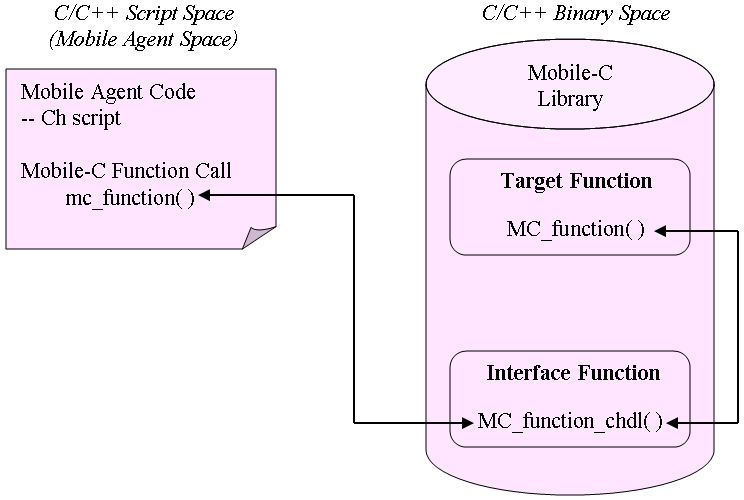
\includegraphics[scale=0.5]{figure/chmobilec_package}
   \caption{Interface of mobile agent code with the Mobile-C library.}
   \label{fig:chmobilec_package}
\end{center}
\end{figure*}
% FIGURE }}}
%%%%%%%%%%%%%%%%%%%%%%%%%%%%%%%%%%%%%%%%%%%%%%%%%%%%%%%%%%%%%%%%%%%%%%
In order to allow mobile agent code to call user defined routines and 
access data sets defined in the binary space, as well as control 
other mobile agents defined in the mobile agent space through the 
Mobile-C API functions, the Mobile-C functionality has to be extended into 
the mobile agent space.
We integrated Ch with the Mobile-C library to provide access to some 
Mobile-C functionalities. 

Figure \vref{fig:chmobilec_package} shows how mobile agent code interfaces 
with the Mobile-C library.
When the function \textit{mc\_function()} is called in mobile agent code,
Ch searches the corresponding interface function \textit{MC\_function\_chdl()} 
in the Mobile-C library, and passes arguments to it by calling the function.
Subsequently, the interface function \textit{MC\_function\_chdl()} invokes the 
target function \textit{MC\_function()}, and passes the return value back to 
the mobile agent space~\cite{EmbeddedCh}.

The prototypes of Mobile-C functions used in the mobile agent space are
declared in \textit{agent.c} through an Embedded Ch function,
\textit{Ch\_DeclareFunc()}.
The data type, \textit{MCAgent\_t}, used as a parameter or return value by 
certain Mobile-C functions for the mobile agent space is also defined in 
\textit{agent.c} by two Embedded Ch functions, 
\textit{Ch\_DeclareVar()} and \textit{Ch\_DeclareTypedef()}~\cite{EmbeddedCh}.
Table \vref{chmobilec_api_cscript} lists the currently implemented functions 
for the mobile agent space.
Two examples are used to demonstrate the applications and features of the 
Mobile-C functionality in the mobile agent space. 

%%%%%%%%%%%%%%%%%%%%%%%%%%%%%%%%%%%%%%%%%%%%%%%%%%%%%%%%%%%%%%%%%%%%%
% Terminate Mobile Agent Execution from Mobile Agent Space {{{
\noindent
\section{Terminate Mobile Agent Execution from Mobile Agent Space}
%%%%%%%%%%%%%%%%%%%%%%%%%%%%%%%%%%%%%%%%%%%%%%%%%%%%%%%%%%%%%%%%%%%%%%
% test2.xml {{{
\begin{Program}[!t]
\begin{center}
   {\footnotesize \linespread{1.0} 
     \verbatiminput{../demos/cspace-agentspace_interface/persistent_example/test2.xml}}
\end{center}
\caption{A mobile agent which enters an infinite loop and does 
  not terminate. \texttt{(<MCPACKAGE>/demos/cspace-agentspace\_interface/persistent\_example/test2.xml)}}
\label{prog:mobileagent1_ex3.xml}
\end{Program}
% }}} test2.xml
%%%%%%%%%%%%%%%%%%%%%%%%%%%%%%%%%%%%%%%%%%%%%%%%%%%%%%%%%%%%%%%%%%%%%%
%%%%%%%%%%%%%%%%%%%%%%%%%%%%%%%%%%%%%%%%%%%%%%%%%%%%%%%%%%%%%%%%%%%%%%
% test3.xml {{{
\begin{Program}[!t]
\begin{center}
   {\footnotesize \linespread{1.0} 
     \verbatiminput{../demos/cspace-agentspace_interface/persistent_example/test3.xml}}
\end{center}
\caption{ This agent terminates the execution
of the agent in Program \ref{prog:mobileagent1_ex3.xml}. 
  \texttt{(<MCPACKAGE>/demos/cspace-agentspace\_interface/persistent\_example/test3.xml)}}
\label{prog:mobileagent2_ex3.xml}
\end{Program}
% }}} test3.xml
%%%%%%%%%%%%%%%%%%%%%%%%%%%%%%%%%%%%%%%%%%%%%%%%%%%%%%%%%%%%%%%%%%%%%%

This example demonstrates how to send a mobile agent to terminate the 
execution of another currently running mobile agent. 
These two mobile agents belong to independent mobile agent spaces. 

The server program used in this example is the same as Program 
\vref{prog:server.c}. 
The client program is the same as Program \vref{prog:client_ex2.c} except 
that it calls the function \textit{MC\_SendAgentMigrationMessageFile()} twice 
to send out two mobile agents.
The first mobile agent sent to the remote agency is 
\textit{test2.xml} shown in Program 
\vref{prog:mobileagent1_ex3.xml}.
The execution of the mobile agent code will repeatedly print a string 
\textit{Hello} to the screen every second.
The second mobile agent sent to the remote agency is 
\textit{test3.xml} shown in Program 
\vref{prog:mobileagent2_ex3.xml}.
The function \textit{mc\_FindAgentByName()} \index{mc\_FindAgentByName()}
returns a variable of type 
\textit{MCAgent\_t} as a handle to a mobile agent. 
The mobile agent code embedded in \textit{mobileagent2\_ex3.xml} finds a 
mobile agent named \textit{mobagent1} by the function 
\textit{mc\_FindAgentByName()} and terminates the execution of 
\textit{mobagent1} by the function \textit{mc\_TerminateAgent()}
\index{mc\_TerminateAgent()}. 
% }}} Terminate Mobile Agent Execution from Mobile Agent Space
%%%%%%%%%%%%%%%%%%%%%%%%%%%%%%%%%%%%%%%%%%%%%%%%%%%%%%%%%%%%%%%%%%%%%%

%%%%%%%%%%%%%%%%%%%%%%%%%%%%%%%%%%%%%%%%%%%%%%%%%%%%%%%%%%%%%%%%%%%%%%
% Invoke a Registered Service from Mobile Agent Space {{{
\noindent
\section{Invoke a Registered Service from Mobile Agent Space}
%%%%%%%%%%%%%%%%%%%%%%%%%%%%%%%%%%%%%%%%%%%%%%%%%%%%%%%%%%%%%%%%%%%%%%
% service_provider_1.xml {{{
\begin{Program}[!t]
\begin{center}
   {\footnotesize \linespread{1.0} 
     \verbatiminput{../demos/agent_space_functionality/mc_df_service_test/service_provider_1.xml}}
\end{center}
\caption{Sample agent containing 'addition' and 'subtraction' services.
Note that the variable ``mc\_current\_agent'' is a special built-in
  variable described in Table
  \vref{tab:agent_space_variables}.\index{mc\_current\_agent}
\texttt{(<MCPACKAGE>/demos/agent\_space\_functionality/mc\_df\_service\_test/ service\_provider\_1.xml)}}
\label{prog:mobileagent1_ex4.xml}
\end{Program}
% }}} service_provider_1.xml
%%%%%%%%%%%%%%%%%%%%%%%%%%%%%%%%%%%%%%%%%%%%%%%%%%%%%%%%%%%%%%%%%%%%%%
%%%%%%%%%%%%%%%%%%%%%%%%%%%%%%%%%%%%%%%%%%%%%%%%%%%%%%%%%%%%%%%%%%%%%%
% service_provider_2.xml {{{
\begin{Program}[!t]
\begin{center}
   {\footnotesize \linespread{1.0} 
     \verbatiminput{../demos/agent_space_functionality/mc_df_service_test/service_provider_2.xml}}
\end{center}
\caption{Sample agent containing 'multiplication' and 'modulus' services.
Note that the variable ``mc\_current\_agent'' is a special built-in
  variable described in Table
  \vref{tab:agent_space_variables}.\index{mc\_current\_agent}
\texttt{(<MCPACKAGE>/demos/mc\_df\_service\_test/service\_provider\_2.xml)}}
\label{prog:mobileagent2_ex4.xml}
\end{Program}
% }}} service_provider_2.xml
%%%%%%%%%%%%%%%%%%%%%%%%%%%%%%%%%%%%%%%%%%%%%%%%%%%%%%%%%%%%%%%%%%%%%%
%%%%%%%%%%%%%%%%%%%%%%%%%%%%%%%%%%%%%%%%%%%%%%%%%%%%%%%%%%%%%%%%%%%%%%
% test2.xml {{{
\begin{Program}[!t]
\begin{center}
   {\scriptsize \linespread{1.0} \verbatiminput{../demos/agent_space_functionality/mc_df_service_test/test1.xml.part1}}
\end{center}
\caption{Sample agent that searches for and invokes agent services.
\texttt{(<MCPACKAGE>/demos/mc\_df\_service\_test/test1.xml)} (Part 1)}
\label{prog:mobileagent3_ex4.xml}
\end{Program}
\addtocounter{Program}{-1}
\begin{Program}[!t]
\begin{center}
   {\scriptsize \linespread{1.0} \verbatiminput{../demos/agent_space_functionality/mc_df_service_test/test1.xml.part2}}
\end{center}
\caption{(Continued) }
\end{Program}
% }}} test2.xml
%%%%%%%%%%%%%%%%%%%%%%%%%%%%%%%%%%%%%%%%%%%%%%%%%%%%%%%%%%%%%%%%%%%%%%

This example demonstrates how to send a mobile agent to invoke a service 
provided by a persistent mobile agent registered with the DF.

The server program used in this example is the same as Program 
\vref{prog:server.c}. 
The client program is the same as Program \vref{prog:client_ex2.c} except 
that it calls the function \textit{MC\_SendAgentMigrationMessageFile()} three
times to send out three mobile agents.
The first mobile agent sent to the remote agency is 
shown in Program 
\vref{prog:mobileagent1_ex4.xml}.
The execution of the mobile agent code will register two services with the 
remote DF through the function mc\_RegisterService(). 
The two services are \textit{addition} and \textit{subtraction} which 
provide addition and subtraction of two integers, respectively.
These services also refer to the functions defined in the mobile agent code.
The function \textit{mc\_RegisterService()} \index{mc\_RegisterService()}
takes three parameters. 
An \textit{MCAgent\_t} type variable is the first parameter. 
A system variable of type \textit{MCAgent\_t}, \textit{mc\_current\_agent}, 
is used as the first parameter when services for 
the current mobile agent are registered, as illustrated in Program 
\vref{prog:mobileagent1_ex4.xml}.
The system variable \textit{mc\_current\_agent} 
is declared in \textit{agent.c} using the function \textit{Ch\_DeclareVar()} 
to hold the current mobile agent.
An array of pointer to char and an integer are the second and third 
parameters, respectively.
The array holds the name of the services whereas the integer denotes the 
number of the services to be registered. 

The second mobile agent is similar to the first and also registers two
services, \textit{multiplication} and \textit{modulus}, which provides 
multiplication and modulo operation of two integers. 
This mobile agent can be seen in Program \vref{prog:mobileagent2_ex4.xml}.

The third mobile agent sent to the remote agency is 
\textit{} shown in Program 
\vref{prog:mobileagent3_ex4.xml}.
The function \textit{mc\_SearchForService()}\index{mc\_SearchForService()} 
takes five parameters.
The first parameter is the name of the service to be found.
The second parameter is the address of an array of ponter to char that 
holds the names of all the mobile agents with the desired service.
Likewise, the third parameter is the address of an array of pointer to 
char that holds the desired service name associated with all the found 
mobile agents.
The fourth parameter is the address of a one-dimensional integer array that 
holds the IDs of all the mobile agents with the desired service.
The last parameter is the address of an integer denoting the number of mobile 
agents that have been found. 
In this example, once the search for \textit{addition} service is done, the 
first mobile agent with this service will be returned by the function 
\textit{mc\_FindAgentByID()}\index{mc\_FindAgentByID()} with a parameter as 
the first element of array \textit{agentIDs}.
In this example, the first found mobile agent is 
\textit{service\_provider\_1}.
The function \textit{addition()} defined in \textit{service\_provider\_1} 
will be called through the function \textit{mc\_CallAgentFunc()} to perform 
addition of two integers.
Since \textit{mc\_CallAgentFunc()}\index{mc\_CallAgentFunc()} can only pass 
one argument to the invoked 
function, the address of a data structure with two integer members is passed 
to \textit{addition()} in this example.
The return value of \textit{addition()} is assigned to the variable 
\textit{retval}.
The string \textit{Result of addition 44 + 45 is 89.} will be printed to the 
screen at the end.   
% }}} Invoke a Mobile Agent Space Function from Mobile Agent Space
%%%%%%%%%%%%%%%%%%%%%%%%%%%%%%%%%%%%%%%%%%%%%%%%%%%%%%%%%%%%%%%%%%%%%%
% }}} Extend Mobile-C Functionality to Mobile Agent Space
%%%%%%%%%%%%%%%%%%%%%%%%%%%%%%%%%%%%%%%%%%%%%%%%%%%%%%%%%%%%%%%%%%%%%%

%%%%%%%%%%%%%%%%%%%%%%%%%%%%%%%%%%%%%%%%%%%%%%%%%%%%%%%%%%%%%%%%%%%%%%
% Synchronization Support int he Mobile-C Library {{{
\chapter{\label{chap:synchronization}Synchronization Support in the Mobile-C library}
In a Mobile-C agency, mobile agents are executed by independent AEEs. 
A user might also need to design a multi-threaded application where a Mobile-C 
agency itself is one of the many threads that handle different tasks.
The Mobile-C library provides support for synchronization among mobile 
agents and threads.
The synchronization API functions are used to protect shared resources as well 
as provide a method of deterministically timing the execution of mobile agents 
and threads.

The internal implementation consists of a linked list of 
Portable Operating System Interface for UNIX (POSIX) compliant synchronization 
variables, namely, mutexes, condition variables, and semaphores. 
Each node in the linked list is a synchronization variable which is assigned 
or given a unique identification number. 
The API functions can be called from the binary or mobile agent 
space to initialize the synchronization variables and access them by their 
unique identification numbers in the linked list.

A Mobile-C synchronization variable is an abstract variable, initialized
by the function {\it MC\_SyncInit()} \index{MC\_SyncInit()}\index{mc\_SyncInit()}.
Once it has been initialized, it may be used as a mutex, condition variable, 
or semaphore.
No further function calls are necessary to change a generic synchronization
variable to one of the types. However, once a synchronization variable is
used as a mutex, condition variable, or semaphore, it should not be used again
as a different type. For instance, if calls to 
\begin{verbatim}
MC_SyncInit(500);
MC_MutexLock(500);
\end{verbatim}
are made, initializing a synchronization variable with ID ``500'', and locking
it as a mutex, it should not be then used with any of the condition variable or
semaphore functions.

The application of the Mobile-C synchronization mechanism is illustrated by 
the example below.

%%%%%%%%%%%%%%%%%%%%%%%%%%%%%%%%%%%%%%%%%%%%%%%%%%%%%%%%%%%%%%%%%%%%%%
% Synchronization in Mobile Agent Space {{{
\noindent
\section{Synchronization in Mobile Agent Space}
%%%%%%%%%%%%%%%%%%%%%%%%%%%%%%%%%%%%%%%%%%%%%%%%%%%%%%%%%%%%%%%%%%%%%%
% client.c {{{
\begin{Program}[!t]
\begin{center}
   {\footnotesize \linespread{1.0} 
     \verbatiminput{../demos/synchronization/agent_mutex_example/client.c}}
\end{center}
\caption{A program used to send a mobile agent. 
  \texttt{(<MCPACKAGE>/demos/synchronization/ agent\_mutex\_example/mc\_client.c)}}
\label{prog:client_ex5.c}
\end{Program}
% }}} client.c
%%%%%%%%%%%%%%%%%%%%%%%%%%%%%%%%%%%%%%%%%%%%%%%%%%%%%%%%%%%%%%%%%%%%%%
%%%%%%%%%%%%%%%%%%%%%%%%%%%%%%%%%%%%%%%%%%%%%%%%%%%%%%%%%%%%%%%%%%%%%%
% sleep.xml {{{
\begin{Program}[!t]
\begin{center}
   {\footnotesize \linespread{1.0} 
     \verbatiminput{../demos/synchronization/agent_mutex_example/sleep.xml}}
\end{center}
\caption{An agent which uses a mutex while accessing a shared resource.
  \texttt{(<MCPACKAGE>/demos/synchronization/agent\_mutex\_example/sleep.xml)} }
\label{prog:mobileagent1_ex5.xml}
\end{Program}
% }}} sleep.xml
%%%%%%%%%%%%%%%%%%%%%%%%%%%%%%%%%%%%%%%%%%%%%%%%%%%%%%%%%%%%%%%%%%%%%%
%%%%%%%%%%%%%%%%%%%%%%%%%%%%%%%%%%%%%%%%%%%%%%%%%%%%%%%%%%%%%%%%%%%%%%
% wake.xml {{{
\begin{Program}[!t]
\begin{center}
   {\footnotesize \linespread{1.0} \verbatiminput{../demos/synchronization/agent_mutex_example/wake.xml}}
\end{center}
\caption{An agent which uses a mutex while accessing a shared resource.
  \texttt{(<MCPACKAGE>/demos/synchronization/agent\_mutex\_example/wake.xml)} }
\label{prog:mobileagent2_ex5.xml}
\end{Program}
% }}} wake.xml
%%%%%%%%%%%%%%%%%%%%%%%%%%%%%%%%%%%%%%%%%%%%%%%%%%%%%%%%%%%%%%%%%%%%%%

The Mobile-C library allows synrchonization among agents via
mutexes, condition variables, and semaphores. Each type of synchronization
variable is used for different features. Perhaps the most common and basic
of these variables is the mutex.

The client program shown in Program \vref{prog:client_ex5.c} starts a Mobile-C
agency listening on port \textit{5050} and subsequently sends two mobile 
agents to 
the remote agency running on host \textit{localhost} at port 
\textit{5051}.
The mobile agents are shown in Program \vref{prog:mobileagent1_ex5.xml} 
and Program \vref{prog:mobileagent2_ex5.xml}. These mobile agents will use
a mutex to guard an operation that may not be performed by two agents
simultaneously.

This example demonstrates the ability of a Mobile-C mutex to protect
a resource that may be shared between two agents. Any real or
imaginary resource that should
not be accessed simultaneously by more than one entity at a time should
be guarded by a mutex. The resource may be a shared variable, or something
more abstract such as control of a robot arm. If there is only one robot arm,
then only one entity, an agent in this case, should be able to control it at a 
time.

In our particular example, the tasks our agents are going to perform are
imaginary. Each task is represented instead by the ``sleep()'' function and
the printing of a message,
which causes execution of that particular agent to pause for a time, as
if it were performing a task. For our example, we will intentionally
cause our agents to collide execution times to demonstrate that our 
mutex works. Examining our client program, Program 
\vref{prog:client_ex5.c},
we see that we set a two second interval between sending the agents. However,
the task that each agent tries to perform will be five seconds long. This
means that the second agent will arrive while the first agent is in the middle
of performing its simulated task. The execution output will demonstrate that
the second agent will not begin its task until the first agent is finished.

Semaphores are also used to guard resources in which a limited number of
entities may access at a time. Since the behaviour and usage of semaphores are
similar to that of a mutex, an example is not provided here. Please see
the demo in directory \texttt{<MCPACKAGE>/demos/agent\_semaphore\_example/} for an example.

\begin{Program}[!t]
\begin{center}
   {\footnotesize \linespread{1.0} \verbatiminput{../demos/synchronization/agent_cond_example/sleep.xml}}
\end{center}
\caption{A sample agent which will immediately sleep on a condition variable
after arriving at an agency. \texttt{(<MCPACKAGE>/demos/synchronization/agent\_cond\_example/sleep.xml)}}
\label{prog:cond_agent_1}
\end{Program}

\begin{Program}[!t]
\begin{center}
   {\footnotesize \linespread{1.0} \verbatiminput{../demos/synchronization/agent_cond_example/wake.xml}}
\end{center}
\caption{A sample agent which will signal a condition variable after arriving
at an agency. \texttt{(<MCPACKAGE>/demos/synchronization/agent\_cond\_example/wake.xml)}}
\label{prog:cond_agent_2}
\end{Program}

Condition variables are also useful in multi-threaded applications in order
for threads to sleep and wait for a signal. Program 
\vref{prog:cond_agent_1} illustrates an agent that will sleep on a condition
  variable immediately after arriving at an agency. Program 
\vref{prog:cond_agent_2} shows an agent that will send a signal to the condition
variable the first agent in Program \ref{prog:cond_agent_1} is waiting on, thereby
causing the first agent to wake up and continue execution.
% }}} Synchronization in the Mobile Agent Space 
%%%%%%%%%%%%%%%%%%%%%%%%%%%%%%%%%%%%%%%%%%%%%%%%%%%%%%%%%%%%%%%%%%%%%%

%%%%%%%%%%%%%%%%%%%%%%%%%%%%%%%%%%%%%%%%%%%%%%%%%%%%%%%%%%%%%%%%%%%%%%
% Synchronization Between Binary and Agent Spaces {{{
%%%%%%%%%%%%%%%%%%%%%%%%%%%%%%%%%%%%%%%%%%%%%%%%%%%%%%%%%%%%%%%%%%%%%%
% server.c {{{
\begin{Program}[!t]
\begin{center}
   {\footnotesize \linespread{1.0} \verbatiminput{../demos/synchronization/cspace_mutex_example/server.c}}
\end{center}
\caption{A sample program with an embedded Mobile-C agency demonstrating the use of a 
Mobile-C mutex to protect a shared resource. \texttt{(<MCPACKAGE>/demos/synchronization/cspace\_mutex\_example/mc\_server.c)}}
\label{prog:binary_sync_example_server}
\end{Program}
% }}} server.c
%%%%%%%%%%%%%%%%%%%%%%%%%%%%%%%%%%%%%%%%%%%%%%%%%%%%%%%%%%%%%%%%%%%%%%

%%%%%%%%%%%%%%%%%%%%%%%%%%%%%%%%%%%%%%%%%%%%%%%%%%%%%%%%%%%%%%%%%%%%%%
% agent.xml {{{
\begin{Program}[!t]
\begin{center}
   {\footnotesize \linespread{1.0} \verbatiminput{../demos/synchronization/cspace_mutex_example/agent.xml}}
\end{center}
\caption{A sample Mobile-C agent which must perform an action on a shared resource
guarded by a Mobile-C mutex. \texttt{(<MCPACKAGE>/demos/synchronization/cspace\_mutex\_example/agent.xml)}}
\label{prog:binary_sync_example_agent}
\end{Program}
% }}} agent.xml
%%%%%%%%%%%%%%%%%%%%%%%%%%%%%%%%%%%%%%%%%%%%%%%%%%%%%%%%%%%%%%%%%%%%%%

\section{Synchronization Between Binary and Agent Spaces}
The synchronization variables initialized using MC\_SyncInit() are accessible
in both agent space and binary space, enabling agents to synchronize with 
binary threads. Again, all three Mobile-C synchronization variable types:
mutexes, condition variables, and semaphores, may be used in both
binary and agent space. 

Referring the example server code in Program
\vref{prog:binary_sync_example_server}, we show a piece of code where
a binary program containing a Mobile-C agency must perform a
subroutine involving a shared resource, protecting it with a mutex. 
The shared resource will
be accessible from both the main() binary thread as well as any agents
which are residing in the agency. As such, the server code 
initializes and uses a mutex to protect the shared resource. In our 
example agent shown in Program \vref{prog:binary_sync_example_agent},
we see that this agent needs to access the same shared resource,
and so it must first lock the mutex before doing so. This example
demonstrates that the mutex will prevent both the agent and binary
thread from accessing the resource simultaneously

%%%%%%%%%%%%%%%%%%%%%%%%%%%%%%%%%%%%%%%%%%%%%%%%%%%%%%%%%%%%%%%%%%%%%%
% server.c {{{
\begin{Program}
\begin{center}
   {\footnotesize \linespread{1.0} \verbatiminput{../demos/synchronization/cspace_cond_example/server.c}}
\end{center}
\caption{An example server containing a thread which will run once each time it
is signalled by another thread or by an agent. 
  \texttt{(<MCPACKAGE>/demos/synchronization/cspace\_cond\_example/mc\_server.c)}}
\label{prog:binary_cond_example_server}
\end{Program}
% }}} server.c
%%%%%%%%%%%%%%%%%%%%%%%%%%%%%%%%%%%%%%%%%%%%%%%%%%%%%%%%%%%%%%%%%%%%%%

%%%%%%%%%%%%%%%%%%%%%%%%%%%%%%%%%%%%%%%%%%%%%%%%%%%%%%%%%%%%%%%%%%%%%%
% agent.xml {{{
\begin{Program}
\begin{center}
   {\footnotesize \linespread{1.0} \verbatiminput{../demos/synchronization/cspace_cond_example/agent.xml}}
\end{center}
\caption{A sample agent which signals a condition variable.
\texttt{(<MCPACKAGE>/demos/synchronization/cspace\_cond\_example/agent.xml)}}
\label{prog:binary_cond_example_agent}
\end{Program}
% }}} agent.xml
%%%%%%%%%%%%%%%%%%%%%%%%%%%%%%%%%%%%%%%%%%%%%%%%%%%%%%%%%%%%%%%%%%%%%%

Referring now to 
Program \vref{prog:binary_cond_example_server} and Program 
\vref{prog:binary_cond_example_agent}, we demonstrate the use of 
Mobile-C condition variables to synchronize an agent with a binary thread.
The binary space thread program shown in Program \ref{prog:binary_cond_example_server}
simply waits on a condition variable. The agent shown in Program
\ref{prog:binary_cond_example_agent} signals the binary space thread
with a call to {\it mc\_CondSignal()}, causing the binary space
thread to run once. 
% }}} Synchronization Between Binary and Agent Spaces
%%%%%%%%%%%%%%%%%%%%%%%%%%%%%%%%%%%%%%%%%%%%%%%%%%%%%%%%%%%%%%%%%%%%%%

%%%%%%%%%%%%%%%%%%%%%%%%%%%%%%%%%%%%%%%%%%%%%%%%%%%%%%%%%%%%%%%%%%%%%%
% Mobile-C Execution with Multiple Agencies {{{
\section{Mobile-C Execution with Multiple Agencies}
%%%%%%%%%%%%%%%%%%%%%%%%%%%%%%%%%%%%%%%%%%%%%%%%%%%%%%%%%%%%%%%%%%%%%%
% server.c {{{
\begin{Program}[!t]
\begin{center}
   {\footnotesize \linespread{1.0} \verbatiminput{../demos/miscellaneous/multiple_agency_example/server.c}}
\end{center}
\caption{An example program containing two Mobile-C agencies. The program
copies agents arriving at the agency on port 5051 to the agency at port
5052.\texttt{(<MCPACKAGE>/demos/miscellaneous/multiple\_agency\_example/mc\_server.c)}}
\label{prog:multiple_agency_server}
\end{Program}
% }}} server.c
%%%%%%%%%%%%%%%%%%%%%%%%%%%%%%%%%%%%%%%%%%%%%%%%%%%%%%%%%%%%%%%%%%%%%%

Using the Mobile-C library, multiple agencies may be initialized 
within the same program. This is useful in cases where the agencies
may have different AEE configuration properties, privileges, etc. 
Ch is the chosen AEE of Mobile-C. 
Functions such as MC\_CopyAgent() and MC\_AddAgent() become useful
in such cases. 

In the example shown in Program \vref{prog:multiple_agency_server},
we demonstrate a program with two agencies, listening on ports
5051 and 5052, respectively. In our simple example, the server
simple duplicates every agent arriving to the agency on port 5051
and adds a copy to the agency on port 5052. 

Note that the 
MC\_CopyAgent() function is necessary here because Mobile-C
functions which retrieve agents from agencies only retrieve references
to the agents, not copies of the agents. The MC\_CopyAgent() function performs
a deep copy on the agent structure so that it may be used in another
agency. Also note that setting the copied agent's status to 
``MC\_WAIT\_CH'' ensures that it will execute again upon entering the 
second agency. 
% }}} Mobile-C Execution with Multiple Agencies
%%%%%%%%%%%%%%%%%%%%%%%%%%%%%%%%%%%%%%%%%%%%%%%%%%%%%%%%%%%%%%%%%%%%%%

% }}} Synchronization Support in the Mobile-C Library
%%%%%%%%%%%%%%%%%%%%%%%%%%%%%%%%%%%%%%%%%%%%%%%%%%%%%%%%%%%%%%%%%%%%%%

%%%%%%%%%%%%%%%%%%%%%%%%%%%%%%%%%%%%%%%%%%%%%%%%%%%%%%%%%%%%%%%%%%%%%%
% {{{ Mobile-C Security Module
\chapter{Mobile-C Security Module \label{chap:Security}}
The Mobile-C package (version 1.10.@@) includes a security module. 
This security module is intended to provide secure migration process of 
  mobile agents and ACL messages from one agency to another. 
Before the migration process, both agencies must authenticate each other 
  successfully. 
After that, an encrypted mobile agent is transferred and its integrity 
  is verified at the receiver side. 
The security module helps guard against man-in-the-middle attacks and
  eavesdropping, and provides a strong authentication of the 
  agencies involved in the migration process.

%%%%%%%%%%%%%%%%%%%%%%%%%%%%%%%%%%%%%%%%%%%%%%%%%%%%%%%%%%%%%%%%%%%%%%
% Security Module Architecture and Overview {{{
\section{Security Module Architecture and Overview}
The Mobile-C security module is inspired by the SSH protocol.
When a security-enabled agency attempts to contact another agency for 
  the migration of a mobile agent or an ACL message, both
  agencies must authenticate each other before the  migration process. 
A successful authentication creates a trust between the two agencies.

Each security-enabled agency must contain a \textit{known\_host} file 
  and a pair of private (\textit{rsa\_priv}) and public (\textit{rsa\_pub}) 
  key files.
These files are provided to each agency by the administrator at 
  startup time. 
The \textit{known\_host} file contains the host name and public key 
  of each agency in the network, as an identifier. 
By default, each agency trusts all the agencies that are listed 
  in the \textit{known\_host} file. 
The \textit{rsa\_priv} and \textit{rsa\_pub} key files contains the 
  private and public key of the agency.

% }}} Security Module Architecture and Overview
%%%%%%%%%%%%%%%%%%%%%%%%%%%%%%%%%%%%%%%%%%%%%%%%%%%%%%%%%%%%%%%%%%%%%%


%%%%%%%%%%%%%%%%%%%%%%%%%%%%%%%%%%%%%%%%%%%%%%%%%%%%%%%%%%%%%%%%%%%%%%
% Enabling the Security Module {{{
\section {Enabling the Security Module}
The configuration options need to be changed in order for the module 
to be built and used are below.
%%%%%%%%%%%%%%%%%%%%%%%%%%%%%%%%%%%%%%%%%%%%%%%%%%%%%%%%%%%%%%%%%%%%%%
% Enabling the Security Module in Unix {{{
\subsection{Enabling the Security Module in Unix}
In a Unix environment, a configuration option needs to be stated during
the configuration process. The new configuration step will be the command
\begin{verbatim}
./configure --enable-security
\end{verbatim}
instead of the old
\begin{verbatim}
./configure
\end{verbatim}

% }}} Enabling the Security Module in Unix
%%%%%%%%%%%%%%%%%%%%%%%%%%%%%%%%%%%%%%%%%%%%%%%%%%%%%%%%%%%%%%%%%%%%%%

%%%%%%%%%%%%%%%%%%%%%%%%%%%%%%%%%%%%%%%%%%%%%%%%%%%%%%%%%%%%%%%%%%%%%
% Enabling the Security Module in Windows {{{
\subsection{Enabling the Security Module in Windows}
For Windows, below is the line that needs to be comment out in the 
file ``[MobileC\_HOME]/src/winconfig.h''.
\begin{verbatim}
#define MC_SECURITY 1
\end{verbatim}
% }}} Enabling the Security Module in Windows
%%%%%%%%%%%%%%%%%%%%%%%%%%%%%%%%%%%%%%%%%%%%%%%%%%%%%%%%%%%%%%%%%%%%%%

%%%%%%%%%%%%%%%%%%%%%%%%%%%%%%%%%%%%%%%%%%%%%%%%%%%%%%%%%%%%%%%%%%%%%%
% Further Instructions {{{
\subsection{Further Instructions}
If the private key file is used in encrypted form then option needs to 
be turned on. 
The following C code snippet will start a security-enabled agency 
  listening on port 5050.
\begin{verbatim}
MCAgency_t agency;
MC_AgencyOptions_t options;
MC_InitializeAgencyOptions(&options);
strcpy(options.passphrase, "alpha1234");
agency = MC_Initialize(5050, &options);

\end{verbatim}

See more about the MC\_AgencyOptions\_t type at the description of the
  MC\_Initialize() function in Appendix A on page \pageref{api:MC_Initialize}.

% }}} Further Instructions
%%%%%%%%%%%%%%%%%%%%%%%%%%%%%%%%%%%%%%%%%%%%%%%%%%%%%%%%%%%%%%%%%%%%%%

% }}} Enabling the Security Module
%%%%%%%%%%%%%%%%%%%%%%%%%%%%%%%%%%%%%%%%%%%%%%%%%%%%%%%%%%%%%%%%%%%%%%

%%%%%%%%%%%%%%%%%%%%%%%%%%%%%%%%%%%%%%%%%%%%%%%%%%%%%%%%%%%%%%%%%%%%%%
% Preparation to Run Security Enabled Agency  {{{
\section{Preparation to Run Security Enabled Agency}
Before running a Mobile-C agency with the security option, 
  the following files are required.
\begin{enumerate}
\item A known host file (\text{known\_host})
\item A pair for public (\textit{rsa\_pub}) and private 
      (\textit{rsa\_priv}) key files
\end{enumerate} 
  are required to be created. 
These are \textit{known\_host} file and \textit{private key} file.  
A small utility source program 
  \begin{verbatim} [MobileC-SRC_HOME]/src/util/mc_keygen.c \end{verbatim} 
  is provided with the Mobile-C library to create a pair of public 
  and private key files for an agency. 
When you make the Mobile-C library the executable for this source program
  can be found in 
  \begin{verbatim} [Mobile-C_HOME]/bin/mc_keygen \end{verbatim}
It is required to create a separate pair of public and private key file
  for each agency. 
That means if there are \textit{n} agencies in a network then \textit{n}
  number of public and private key file pairs are required.
The private key files can be created in plaintext or encrypted 
  form. Details can be found in section 9.3.1.
The known host file needs to be built manually after creating public
  and private key files.

%%%%%%%%%%%%%%%%%%%%%%%%%%%%%%%%%%%%%%%%%%%%%%%%%%%%%%%%%%%%%%%%%%%%%%
% Generating Key Files {{{
\subsection{Generating Key Files}
A utility program {\bf mc\_genkey} \textit{([MobileC-Home]/bin/mc\_genkey)} is 
used to create public and private key files.
This utility program can create a private key in plain text or cipher text.
To generate the key files with private key in plain text, you can execute the 
{\bf mc\_genkey} as 
\begin{verbatim}
$./mc_genkey -rsakeys -pt
Seeding the random number generator 
Generating the RSA key [ 1024-bit ] 
Exporting public key in rsa_pub 
Exporting the private key in rsa_priv 
Done. 
Key generated.
\end{verbatim}
where \textit{-pt} means to generate private key in plain text. 
Similarly,
\begin{verbatim}
$./mc_genkey -rsakeys -en
Enter Passphrase (A-Z, a-z, 0-9)to encrypt privatekey file
(remember your passphrase otherwise encrypted private key file is useless)
>  alpha1234

Seeding the random number generator 
Generating the RSA key [ 1024-bit ] 
Exporting public key in rsa_pub 
Exporting the private key in rsa_priv 
encrypted. 
done. 
keys generated.
\end{verbatim}

would generate the private key in encrypted form, where \textit{en} stands 
for encryption. 
Here we a passphrase (\textit{alpha1234})is provided to encrypt the private 
  key file. 
With this option it prompts for the passphrase that is used to encrypt the 
  rsa private key. 
Here we entered a passphrase (\textit{alpha1234}) to encrypt the private 
  key file.
You can enter a string maximum upto 32 bytes in length consisting of small 
  or capital alphabet and/or 1-9 digits. 
The same passphrase is required by the Mobile-C agency to decrypt the 
  private key file.
With both options, it generates the public key file in plain text.
The output file names are \textit{rsa\_pub} for public key and
\textit{rsa\_priv} for private key.

% }}} Generating Key Files
%%%%%%%%%%%%%%%%%%%%%%%%%%%%%%%%%%%%%%%%%%%%%%%%%%%%%%%%%%%%%%%%%%%%%%

%%%%%%%%%%%%%%%%%%%%%%%%%%%%%%%%%%%%%%%%%%%%%%%%%%%%%%%%%%%%%%%%%%%%%%
% FIGURE {{{ 
\begin{figure*}[!t]
\begin{center}
   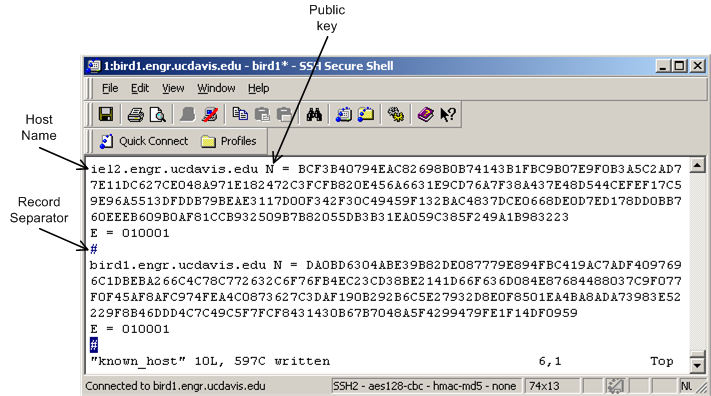
\includegraphics[scale=0.5]{figure/knownhost}
   \caption{A sample known host file.}
   \label{fig:knownhost}
\end{center}
\end{figure*}
% FIGURE }}}
%%%%%%%%%%%%%%%%%%%%%%%%%%%%%%%%%%%%%%%%%%%%%%%%%%%%%%%%%%%%%%%%%%%%%%

%%%%%%%%%%%%%%%%%%%%%%%%%%%%%%%%%%%%%%%%%%%%%%%%%%%%%%%%%%%%%%%%%%%%%%
% Known Host file {{{
\subsection{Known Host File}
After creating the key files for all the agencies in a network the 
  \textit{known\_host} file needs to be created manully.
The sample \textit{known\_host} file is shown in Figure ~\ref{fig:knownhost}. 
To proceed, create a file using a text editor with name 
  \textit{known\_host}. 
Type the name of the first agency (as shown \textit{Host Name} in 
Figure ~\ref{fig:knownhost}) and 
copy its public key from \textit{rsa\_pub} file. Insert the record 
separation character \# and type the same for second agency and continue.
Make sure that the name for the \textit{known\_host} file is 
\textit{``known\_host"}. After creating the 
\textit{known\_host} file, copy the \textit{known\_host} file to each \
agency and the \textit{rsa\_priv} file on the respective
agencies (the same directory from where you will run the Mobile-C 
agency). 
Public and private key files are always created as a pair this means that
  any text encrypted with the public key can only be decrypted with the
  corresponding (paired) private key.
Therefore, please make sure that the copied private key 
(\textit{rsa\_priv}) to an agency must correspond to the public key
that is mentioned infront of the name of this agency in \textit{
known\_host} file.
% }}} Known Host File
%%%%%%%%%%%%%%%%%%%%%%%%%%%%%%%%%%%%%%%%%%%%%%%%%%%%%%%%%%%%%%%%%%%%%%

%}}} Preparation to Run Security Enabled Agency
%%%%%%%%%%%%%%%%%%%%%%%%%%%%%%%%%%%%%%%%%%%%%%%%%%%%%%%%%%%%%%%%%%%%%

%%%%%%%%%%%%%%%%%%%%%%%%%%%%%%%%%%%%%%%%%%%%%%%%%%%%%%%%%%%%%%%%%%%%%
% Examples {{{
\section{Examples -- Mobile-C Security}
A Mobile-C security enable agency can be executed with encypted or plaintext
  private key. 
When you execute a Mobile-C agency it will look for private key file named
  \textit{rsa\_priv} in the current directory. 
If the private key is encrypted and the passphrase is not provided in Mobile-C
  agency C program then it will prompt for the passphrase.
\texttt{<MCPACKAGE>/demos/} contains two demos 
  (\textit{hello\_world\_secure} and \textit{multi\_task\_example\_secure}) that 
  uses private key in plain text.

Please note that for \textit{hello\_world\_secure} demo, the private and public
  key pair is same for client and server, that is both the client and server 
  program run on the same machine (iel2.engr.ucdavis.edu).
To run the demo in your machine, you to write the name of your machine in 
  \textit{known\_host} file and the mobile agent file (\textit{test1.xml}) 

To run client and server agencies on the two different machines, you need to
  create a pair of public and private keys (see section 9.3.1) and that 
  is for the second machine.  
The first agency can use the already created key files that are provided with
  demos.
After creating the key files, edit the \textit{known\_host} file by including
  the name of other machine and newly created public key from file 
  (\textit{rsa\_priv}), for details see section 9.3.2.
Also copy the newly generated private key file (\textit{rsa\_priv}) and 
  updated \textit{known\_host} file on the other machine in the same 
  directory from where Mobile-C agency will be executed.
Now start the server program and then the client program.

Please note that when you build the demos, the executable 
 files ( \textit{client} and  \textit{server}) for demo 
 \textit{hello\_world \_secure} are in 
 directories \textit{hello\_world\_secure/client} and 
 \textit{hello\_world\_ secure/server} respectively. Similarly, the executable 
 files (\textit{client},  \textit{server1} and  \textit{server2} ) for demo
  \textit{multi\_task\_example\_secure} are in directories 
   \textit{multi\_task\_e xample\_secure/client}, 
   \textit{multi\_task\_example\_secure/server1} and
   \textit{multi\_task\_example\_secure/server2} respectively.

Each agency uses a separate \textit{known\_host},
  public(\textit{rsa\_pub}) and private key {\textit{rsa\_priv} pair files. 

\begin{Program}[!t]
\begin{center}
   {\footnotesize \linespread{1.0} \verbatiminput{../demos/mobilec_security/hello_world_secure/server.c }}
\end{center}
\caption{ A sample server side code for security enable agency 
       (\textit{../demos/mobilec\_security/hello\_world\_secure/server.c})}
\label{prog:security_server}
\end{Program}

\begin{Program}[!t]
\begin{center}
   {\footnotesize \linespread{1.0} \verbatiminput{../demos/mobilec_security/hello_world_secure/client.c }}
\end{center}
\caption{ A sample client side code for security enable agency
        (\textit{../demos/mobilec\_security/hello\_world\_secure/client.c})}
\label{prog:security_client}
\end{Program}

The programs \ref{prog:security_server} and \ref{prog:security_client} show 
  \textit{hello\_world\_secure} server and client code respectively.
Please note that the \textit{MC\_AgencyOptions\_t} is required only if the 
  private key file is encrypted. 
Since both programs use the private key file (\textit{rsa\_priv}) in plaintext
  so \textit{MC\_AgencyOptions\_t} is NULL in \textit{MC\_Initialize} function.

If you generate the private key file (\textit{rsa\_priv}) in encrypted form 
   (see section 9.3.1) then the Mobile-C agency requires the same passphrase 
    to decrypt its private key that you have entered to encrypted this file.
In this case \textit{MC\_AgencyOptions\_t} should not be NULL. 
It is a possible that passphrase would not be privided in the code. 
That is, this code can be run if 
  \textit{strcpy(options.passphrase, "xxxx");} is commented out.
In this case, if the private key is encyrpted the Mobile-C agency
  would prompt to enter passphrase at startup otherwise not. 

%To run the these programs in your machine you need to replace 
%  \textit{rabbit.engr.ucdavis.edu} to your machine name in 
%  \textit{client.c}, \textit{test1.xml} and \textit{known\_host}
%  file.
%The \textit{test1.xml} is a hello world mobile agent. \
     

% }}} Example


%%%%%%%%%%%%%%%%%%%%%%%%%%%%%%%%%%%%%%%%%%%%%%%%%%%%%%%%%%%%%%%%%%%%%%

% }}} Mobile-C Security Module
%%%%%%%%%%%%%%%%%%%%%%%%%%%%%%%%%%%%%%%%%%%%%%%%%%%%%%%%%%%%%%%%%%%%%%

%%%%%%%%%%%%%%%%%%%%%%%%%%%%%%%%%%%%%%%%%%%%%%%%%%%%%%%%%%%%%%%%%%%%%%
%{{{Communication With Other FIPA Compliant Agent Systems
\chapter{Communication With Other FIPA Compliant Agent Systems}
This section provides some brief examples regarding communication
between Mobile-C and other FIPA compliant agent systems.
\subsection{Example: Receiving a message from a JADE agent}
The following section contains details regarding an example where a
Mobile-C agent receives a message from a JADE agent. This example is
included to provide a brief overview of how FIPA ACL communication
operates between Mobile-C agencies and JADE agencies.

\subsubsection{Start a Mobile-C Agency}
The first step in the example is to start a Mobile-C agency and a suitable
agent to wait for a message. An example agency which performs these tasks
may be found in the directory \texttt{<MCPACKAGE>/demos/ jade\_to\_mc\_example/}.
To start the agency, simply go to the directory and execute the server
with the command
\begin{verbatim}
./server
\end{verbatim}
The server will start and load the sample agent named ``mobagent1'' in one step,
which should produce the following output (or similar):
\begin{verbatim}
Mobile-C Started

MobileC > This is mobagent1 from the agency at port 5050.
Now, I am going to wait until I receive a message. Waiting...
\end{verbatim}

\subsubsection{Create a JADE container}
The next step is to start a JADE agency. Instructions on how to obtain and
install JADE may be found at the website \texttt{<http://jade.tilab.com>} .
Once JADE in installed, use the command
\begin{verbatim}
java jade.Boot -gui
\end{verbatim}
to start a JADE container. Note that the command may vary across systems depending
on your java distribution and system setup. This command should produce a window
similar to the following:

\begin{center}
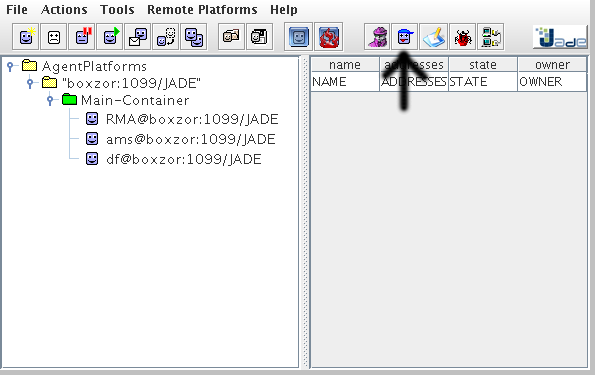
\includegraphics[width=4in]{figure/jade_to_mc_example/jade_main_window.png}
\end{center}

\subsubsection{Start a JADE dummy agent}
The next step is to start a ``dummy'' agent by clicking on the button indicated by the 
large arrow in the previous figure. This should produce a second window
which should resemble the following image.

\begin{center}
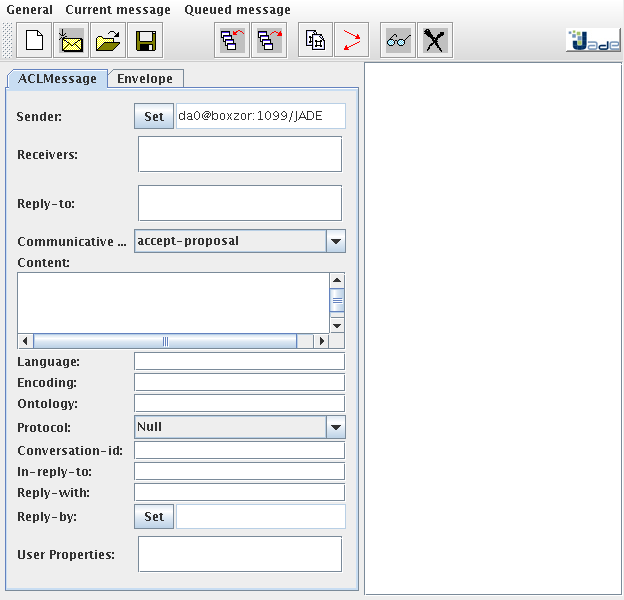
\includegraphics[width=4in]{figure/jade_to_mc_example/dummy_agent_window_blank.png}
\end{center}

\subsubsection{Send a message to Mobile-C}
There are several fields in this empty ACL message that need to be set before the
message will be successfully passed to our Mobile-C agent. The first field to fill
out is the \texttt{Receivers}, which indicates the recipients for our message.
We wish for our Mobile-C agent ``mobagent1'' to be our sole recipient. Add 
``mobagent1'' by right-clicking on the \texttt{Receivers} textbox and selecting the
\texttt{Add} option. Fill out the box as shown in the following image:

\begin{center}
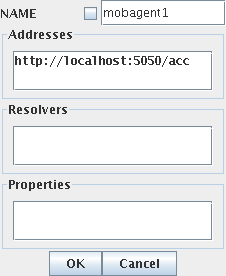
\includegraphics[width=2in]{figure/jade_to_mc_example/dummy_agent_receiver_window.png}
\end{center}

After setting the receiver, the rest of the message may be set to whatever is desired.
For this example, our sample message may be seen on the following image.

\begin{center}
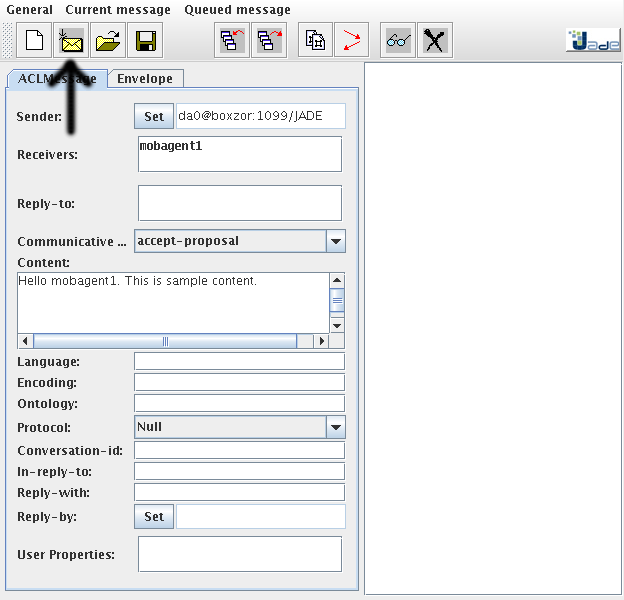
\includegraphics[width=4in]{figure/jade_to_mc_example/dummy_agent_window_complete.png}
\end{center}

Once your desired message parameters are in place, click on the ``Send Message'' button
indicated by the arrow in the previous figure. The message will be sent to the agent
waiting at the Mobile-C agency that was previously started. The agent should
receive the message and produce the following output:
\begin{verbatim}
mobagent1 Got a message!
Message is from da0@boxzor:1099/JADE
The content is Hello mobagent1. This is sample content.
\end{verbatim}
This indicates that \texttt{mobagent1} has successfully received the
message from JADE.

\subsection{Example: Sending a message from Mobile-C to JADE}
This example illustrates a Mobile-C agent sending an ACL message to a
JADE agent.  The example will be presented in a step by step fashion and all
files may be found in the directory \texttt{<MCPACKAGE>/demos/mc\_to\_jade\_example/}.

\subsubsection{Start a JADE container with a ``PingAgent'' agent}
The first step is to start a JADE container with a responsive agent. In this
example, we will use a demo ``PingAgent'' agent which is provided with JADE. The
agent source code may be found in the JADE subdirectory 
\texttt{jade/src/examples/PingAgent/PingAgent.java} . After installing JADE,
run the command
\begin{verbatim}
java jade.Boot pingme:examples.PingAgent.PingAgent
\end{verbatim}
from the \texttt{jade/src/} directory to start a JADE main container and 
invoke an agent of type ``PingAgent'' named ``pingme''. The ``PingAgent'' agent
contains a behaviour which receives messages and replies with a standard 
reply message. The ``PingAgent'' expects incoming messages to have a performative
of ``query-ref'', and for the content field to contain the text ``ping''. 

\subsubsection{Start a Mobile-C agency with a sender agent}
A Mobile-C agency and agent for use in the example has already been
created and reside in the directory \texttt{<MCPACKAGE>/demos/mc\_to\_jade\_example/} .
After compiling Mobile-C and the Mobile-C demos, simply go to the directory and
run the 'client' executable.
\begin{verbatim}
./client
\end{verbatim}
The executable will automatically start a Mobile-C agency and load an agent
named ``mobagent1''. The agent is programmed to send an ACL message to 
``pingme'' at the local JADE container and wait for a response message. 
Upon receiving the response, the agent will print the contents of the 
response message. The Mobile-C agent output should look something like
\begin{verbatim}
Mobile-C Started
Sending agent to self...
Done.
mobagent2 Creating new ACL message...
mobagent2 sending ACL message...
Received a message from pingme@boxzor:1099/JADE.
Content is 'alive'.
\end{verbatim}
%}}}
%%%%%%%%%%%%%%%%%%%%%%%%%%%%%%%%%%%%%%%%%%%%%%%%%%%%%%%%%%%%%%%%%%%%%%

%%%%%%%%%%%%%%%%%%%%%%%%%%%%%%%%%%%%%%%%%%%%%%%%%%%%%%%%%%%%%%%%%%%%%%
% Bibliography {{{
%\phantomsection
%\addcontentsline{toc}{chapter}{Bibliography}
\bibliographystyle{IEEEtran}
%\bibliography{/home/chgroup/project/paper/ielpaper}
\bibliography{ielpaper}
\pagebreak
% }}} Bibliography 
%%%%%%%%%%%%%%%%%%%%%%%%%%%%%%%%%%%%%%%%%%%%%%%%%%%%%%%%%%%%%%%%%%%%%%

%%%%%%%%%%%%%%%%%%%%%%%%%%%%%%%%%%%%%%%%%%%%%%%%%%%%%%%%%%%%%%%%%%%%%%
% Appendix {{{
\appendix
\chapter{Mobile-C API in the C/C++ Binary Space \label {appendix}}
\lhead{Mobile-C API in the C/C++ Binary Space}
\noindent
The header file {\bf libmc.h} defines all the data types, macros 
and function prototypes for the Mobile-C library.
The header file is used in the C/C++ binary space.

\begin{table}[!h]
\capstart
\begin{center}
\caption{Data types defined in {\bf libmc.h}.}
\begin{tabular}{p{50 mm}p{110 mm}}
\hline
Data Type & Description \\
\hline
{\bf MCAgency\_t} & A handle containing information of an agency. \\
{\bf MCAgent\_t} & A handle containing information of a mobile agent. \\
{\bf MCAgencyOptions\_t} & A structure containing information about which thread(s) to be activated and the default agent status specified by a user. \\
\hline
\end{tabular}
\end{center}
\label{mobilec_datatype}
\end{table}

The header file {\bf fipa\_acl.h} contains datatype and macros related to 
FIPA ACL messaging, as described in Chapter \ref{chap:fipa}. This header
file may be used in both C/C++ binary space, as well as agent space.

\begin{table}[!h]
\capstart
\begin{center}
\caption{Data types defined in {\bf fipa\_acl.h}.}
\begin{tabular}{p{50 mm}p{110 mm}}
\hline
Data Type & Description \\
\hline
{\bf fipa\_acl\_message\_t} & A structure containing a FIPA ACL message. \\
\hline
\end{tabular}
\end{center}
\label{fipa_datatype}
\end{table}

\pagebreak

\begin{table}[!h]
\capstart
\begin{center}
\caption{Macros defined in {\bf libmc.h}.}
\begin{tabular}{p{50 mm}p{110 mm}}
\hline
Macro & Description \\
\hline
{\texttt enum MC\_ThreadIndex\_e} & \\
\hline
{\bf MC\_THREAD\_AI} \index{MC\_THREAD\_AI} & Identifier for agent initalizing thread. \\
{\bf MC\_THREAD\_AM} \index{MC\_THREAD\_AM} & Identifier for agent managing thread. \\
{\bf MC\_THREAD\_CL} \index{MC\_THREAD\_CL} & Identifier for connection listening thread. \\
{\bf MC\_THREAD\_MR} \index{MC\_THREAD\_MR} & Identifier for message receiving thread. \\
{\bf MC\_THREAD\_MS} \index{MC\_THREAD\_MS} & Identifier for message sending thread. \\
{\bf MC\_THREAD\_CP} \index{MC\_THREAD\_CP} & Identifier for command prompt thread. \\
{\bf MC\_THREAD\_ALL} \index{MC\_THREAD\_ALL} & Identifier for all threads. \\
\hline
{\texttt enum MC\_Signal\_e} & \\
\hline
{\bf MC\_RECV\_CONNECTION} \index{MC\_RECV\_CONNECTION} & Signal activated after an agency accepts a connection. \\
{\bf MC\_RECV\_MESSAGE} \index{MC\_RECV\_MESSAGE} & Signal activated after an agency receives an ACL message. \\
{\bf MC\_RECV\_AGENT} \index{MC\_RECV\_AGENT} & Signal activated after an agency receives a mobile agent. \\
{\bf MC\_RECV\_RETURN} \index{MC\_RECV\_RETURN} & Signal activated after an agency receives return data from a completed mobile agent. \\
{\bf MC\_EXEC\_AGENT} \index{MC\_EXEC\_AGENT} & Signal activated after a mobile agent is executed. \\
{\bf MC\_ALL\_SIGNALS} \index{MC\_ALL\_SIGNALS} & Signal activated after any of the above four events occurs. \\
\hline
{\texttt enum MC\_AgentType\_e} \index{MC\_AgentType\_e}& \\
\hline
{\bf MC\_REMOTE\_AGENT} \index{MC\_REMOTE\_AGENT} & Identifier for a remote mobile agent. \\
{\bf MC\_LOCAL\_AGENT} \index{MC\_LOCAL\_AGENT} & Identifier for a local mobile agent.\\
{\bf MC\_RETURN\_AGENT} \index{MC\_RETURN\_AGENT} & Identifier for a return mobile agent. \\
\hline
{\texttt enum MC\_AgentStatus\_e} \index{MC\_AgentStatus\_e} & \\
\hline
{\bf MC\_WAIT\_CH} \index{MC\_WAIT\_CH} & Value indicating a mobile agent is waiting to be executed. \\
{\bf MC\_WAIT\_MESSGSEND} \index{MC\_WAIT\_MESSGSEND}& Value indicating a mobile agent is waiting to be exported to another agency. \\
{\bf MC\_AGENT\_ACTIVE} \index{MC\_AGENT\_ACTIVE}& Value indicating a mobile agent is being executed. \\
{\bf MC\_AGENT\_NEUTRAL} \index{MC\_AGENT\_NEUTRAL}& Value indicating a mobile agent is waiting for an unspecified reason. \\
{\bf MC\_AGENT\_SUSPENDED} \index{MC\_AGENT\_SUSPENDED}& Value indicating a mobile agent is being suspended. \\
{\bf MC\_WAIT\_FINISHED} \index{MC\_WAIT\_FINISHED}& Value indicating a mobile agent has been executed and is waiting to be removed. \\
\hline
\end{tabular}
\end{center}
\label{mobilec_macro}
\end{table}

\begin{table}[!hp]
\capstart
\begin{center}
\caption{Macros defined in {\bf fipa\_acl.h}. Detailed documentation for the
FIPA performatives and protocols may be found in the FIPA specifications at
\texttt{http://www.fipa.org}.}
\begin{tabular}{p{90 mm}p{70 mm}}
\hline
Macro & Description \\
\hline
{\texttt fipa\_performative\_e \index{fipa\_performative\_e}} & \\
\hline
{\bf FIPA\_ACCEPT\_PROPOSAL} \index{FIPA\_ACCEPT\_PROPOSAL} & The \texttt{accept-proposal} performative. \\
{\bf FIPA\_AGREE} \index{FIPA\_AGREE} & The \texttt{agree} performative. \\
{\bf FIPA\_CANCEL} \index{FIPA\_CANCEL} & The \texttt{cancel} performative. \\
{\bf FIPA\_CALL\_FOR\_PROPOSAL} \index{FIPA\_CALL\_FOR\_PROPOSAL} & The \texttt{call-for-proposal} performative. \\
{\bf FIPA\_CONFIRM} \index{FIPA\_CONFIRM} & The \texttt{confirm} performative. \\
{\bf FIPA\_DISCONFIRM} \index{FIPA\_DISCONFIRM} & The \texttt{disconfirm} performative. \\
{\bf FIPA\_FAILURE} \index{FIPA\_FAILURE} & The \texttt{failure} performative. \\
{\bf FIPA\_INFORM} \index{FIPA\_INFORM} & The \texttt{inform} performative. \\
{\bf FIPA\_INFORM\_IF} \index{FIPA\_INFORM\_IF} & The \texttt{inform-if} performative. \\
{\bf FIPA\_INFORM\_REF} \index{FIPA\_INFORM\_REF} & The \texttt{inform-ref} performative. \\
{\bf FIPA\_NOT\_UNDERSTOOD} \index{FIPA\_NOT\_UNDERSTOOD} & The \texttt{not-understood} performative. \\
{\bf FIPA\_PROPOGATE} \index{FIPA\_PROPOGATE} & The \texttt{propogate} performative. \\
{\bf FIPA\_PROPOSE} \index{FIPA\_PROPOSE} & The \texttt{propose} performative. \\
{\bf FIPA\_PROXY} \index{FIPA\_PROXY} & The \texttt{proxy} performative. \\
{\bf FIPA\_QUERY\_IF} \index{FIPA\_QUERY\_IF} & The \texttt{query-if} performative. \\
{\bf FIPA\_QUERY\_REF} \index{FIPA\_QUERY\_REF} & The \texttt{query-ref} performative. \\
{\bf FIPA\_REFUSE} \index{FIPA\_REFUSE} & The \texttt{refuse} performative. \\
{\bf FIPA\_REJECT\_PROPOSAL} \index{FIPA\_REJECT\_PROPOSAL} & The \texttt{reject-proposal} performative. \\
{\bf FIPA\_REQUEST} \index{FIPA\_REQUEST} & The \texttt{request} performative. \\
{\bf FIPA\_REQUEST\_WHEN} \index{FIPA\_REQUEST\_WHEN} & The \texttt{request-when} performative. \\
{\bf FIPA\_REQUEST\_WHENEVER} \index{FIPA\_REQUEST\_WHENEVER} & The \texttt{request-whenever} performative. \\
{\bf FIPA\_SUBSCRIBE} \index{FIPA\_SUBSCRIBE} & The \texttt{subscribe} performative. \\
\hline
{\texttt enum fipa\_protocol\_e} & \\
\hline
{\bf FIPA\_PROTOCOL\_REQUEST} \index{FIPA\_PROTOCOL\_REQUEST} & The FIPA \texttt{request} protocol. \\
{\bf FIPA\_PROTOCOL\_QUERY} \index{FIPA\_PROTOCOL\_QUERY} & The FIPA \texttt{query} protocol. \\
{\bf FIPA\_PROTOCOL\_REQUEST\_WHEN} \index{FIPA\_PROTOCOL\_REQUEST\_WHEN} & The FIPA \texttt{request-when} protocol. \\
{\bf FIPA\_PROTOCOL\_CONTRACT\_NET} \index{FIPA\_PROTOCOL\_CONTRACT\_NET} & The FIPA \texttt{contract-net} protocol. \\
{\bf FIPA\_PROTOCOL\_ITERATED\_CONTRACT\_NET} \index{FIPA\_PROTOCOL\_ITERATED\_CONTRACT\_NET} & The FIPA \texttt{iterated-contract-net} protocol. \\
{\bf FIPA\_PROTOCOL\_ENGLISH\_AUCTION} \index{FIPA\_PROTOCOL\_ENGLISH\_AUCTION} & The FIPA \texttt{english-auction} protocol. \\
{\bf FIPA\_PROTOCOL\_DUTCH\_AUCTION} \index{FIPA\_PROTOCOL\_DUTCH\_AUCTION} & The FIPA \texttt{dutch-auction} protocol. \\
{\bf FIPA\_PROTOCOL\_BROKERING} \index{FIPA\_PROTOCOL\_BROKERING} & The FIPA \texttt{brokering} protocol. \\
{\bf FIPA\_PROTOCOL\_RECRUITING} \index{FIPA\_PROTOCOL\_RECRUITING} & The FIPA \texttt{recruiting} protocol. \\
{\bf FIPA\_PROTOCOL\_SUBSCRIBE} \index{FIPA\_PROTOCOL\_SUBSCRIBE} & The FIPA \texttt{subscribe} protocol. \\
{\bf FIPA\_PROTOCOL\_PROPOSE} \index{FIPA\_PROTOCOL\_PROPOSE} & The FIPA \texttt{propose} protocol. \\
{\bf FIPA\_PROTOCOL\_END} \index{FIPA\_PROTOCOL\_END} & The FIPA \texttt{end} protocol. \\
\hline
\end{tabular}
\end{center}
\label{fipa_macro}
\end{table}

\begin{table}[!hp]
\capstart
\begin{center}
\caption{Functions in the C/C++ binary space.}
\begin{tabular}{p{78 mm}p{77 mm}}
%\begin{tabular}{ll}
\hline
Function & Description \\
\hline
{\bf MC\_AclAddReceiver()} \dotfill & Add a receiver to an ACL message. \\
{\bf MC\_AclAddReplyTo()} \dotfill & Add a reply-to address to an ACL message. \\
{\bf MC\_AclGetContent()} \dotfill & Get the content of an ACL message. \\
{\bf MC\_AclGetConversationID()} \dotfill & Get the conversation id from an ACL message. \\
{\bf MC\_AclGetPerformative()} \dotfill & Get the performative of an ACL message. \\
{\bf MC\_AclGetProtocol()} \dotfill & Get the protocol from an ACL message. \\
{\bf MC\_AclGetSender()} \dotfill & Get the sender of an ACL message. \\
{\bf MC\_AclNew()} \dotfill & Allocate a new FIPA ACL message. \\
{\bf MC\_AclPost()} \dotfill & Post a FIPA ACL message to an agent's mailbox. \\
{\bf MC\_AclReply()} \dotfill & Allocate a new FIPA ACL message automatically addressed to the sender of a previous message. \\
{\bf MC\_AclRetrieve()} \dotfill & Retrieve an ACL message from an agent's mailbox. \\
{\bf MC\_AclSetContent()} \dotfill & Set the content of an ACL message. \\
{\bf MC\_AclSetConversationID()} \dotfill & Set the conversation id of an ACL message. \\
{\bf MC\_AclSetPerformative()} \dotfill & Set the performative of an ACL message. \\
{\bf MC\_AclSetProtocol()} \dotfill & Set the protocol of an ACL message. \\
{\bf MC\_AclSetSender()} \dotfill & Set the sender of an ACL message. \\
{\bf MC\_AclWaitRetrieve()} \dotfill & Wait for a message to arrive at an agent's mailbox. \\
{\bf MC\_AgentAddTask()} \dotfill & Add a task to an agent based off of C source code. \\
{\bf MC\_AgentAddTaskFromFile()} \dotfill & Add a task to an agent based off of a C source code file. \\
{\bf MC\_AgentAttachFile()} \dotfill & Attach a file to the agent's current task. \\
{\bf MC\_AgentListFiles()} \dotfill & List files attached to an agent's task. \\
{\bf MC\_AgentRetrieveFile()} \dotfill & Retrieve and save an agent's attached file onto the filesystem. \\
{\bf MC\_AgentReturnArrayDim()} \dotfill & Get the dimension of an array returned by an agent. \\
{\bf MC\_AgentReturnArrayExtent()} \dotfill & Get the extent of a dimension of an array returned by an agent. \\
{\bf MC\_AgentReturnArrayNum()} \dotfill & Get the number of elements of an array returned by an agent. \\
{\bf MC\_AgentReturnDataGetSymbolAddr()} \dotfill & Get a pointer to an array returned by an agent. \\
{\bf MC\_AgentReturnDataSize()} \dotfill & Get the size of a single element of the array. \\
{\bf MC\_AgentReturnDataType()} \dotfill & Get the type of the array. \\
{\bf MC\_AgentReturnIsArray()} \dotfill & Determine if the returned variable is an array. \\
{\bf MC\_AddAgent()} \dotfill & Add a mobile agent into an agency. \\
{\bf MC\_AddAgentInitCallback()} \dotfill & Add an agent initialization callback function into an agency. \\
{\bf MC\_AddStationaryAgent()} \dotfill & Add a mobile agent into an agency. \\
%{\bf MC\_AgentVariableRetrieve()} & Retrieve a saved variable from an agent's prior task. \\
%{\bf MC\_AgentVariableSave()} & Save an agent's task variable for migration. \\
{\bf MC\_Barrier()} \dotfill & Block until all agents in an agency have called this function. \\
{\bf MC\_BarrierDelete()} \dotfill & Delete a Mobile-C barrier. \\
{\bf MC\_BarrierInit()} \dotfill & Initialize a Mobile-C barrier. \\
{\bf MC\_CallAgentFunc()} \dotfill & Call a function defined in an agent. \\
{\bf MC\_CallAgentFuncV()} \dotfill & Call a function defined in an agent. \\
\hline
\end{tabular}
\end{center}
\label{mobilec_api_cbinary}
\end{table}

\addtocounter{table}{-1}
\begin{table}[!hp]
\capstart
\begin{center}
\caption{Functions in the C/C++ binary space (contd.).}
%\begin{tabular}{ll}
\begin{tabular}{p{78 mm}p{77 mm}}
\hline
Function & Description \\
\hline
{\bf MC\_CallAgentFuncVar()} \dotfill & Call a function defined in an agent. \\
{\bf MC\_ChInitializeOptions()} \dotfill & Set the initialization options for a Ch to be used as one AEE in an agency. \\
{\bf MC\_ComposeAgent()} \dotfill & Compose an agent from program source code. \\
{\bf MC\_ComposeAgentS()} \dotfill & [Deprecated] Compose an agent from program source code with a workgroup code. \\
{\bf MC\_ComposeAgentWithWorkgroup()} \dotfill & Compose an agent from program source code with a workgroup code. \\
{\bf MC\_ComposeAgentFromFile()} \dotfill & Compose an agent from a program source code file. \\
{\bf MC\_ComposeAgentFromFileS()} \dotfill & [Deprecated] Compose an agent from a program source code file with a workgroup code. \\
{\bf MC\_ComposeAgentFromFileWithWorkgroup()} & Compose an agent from a program source code file with a workgroup code. \\
{\bf MC\_CondBroadcast()} \dotfill & Wake up all agents/threads waiting on a condition variable. \\
{\bf MC\_CondReset()} \dotfill & Reset a Mobile-C condition variable. \\
{\bf MC\_CondSignal()} \dotfill & Signal another agent that is waiting on a condition variable. \\
{\bf MC\_CondWait()} \dotfill & Cause the calling agent or thread to wait on a Mobile-C condition variable with the ID specified by the argument. \\
{\bf MC\_CopyAgent()} \dotfill & Perform a deep copy to copy an agent. \\
{\bf MC\_DeleteAgent()} \dotfill & Stop and remove an agent from an agency. \\
{\bf MC\_DeregisterService()} \dotfill & Deregister a service with the Directory Facilitator. \\
{\bf MC\_End()} \dotfill & Terminate a Mobile-C agency. \\
{\bf MC\_FindAgentByID()} \dotfill & Find a mobile agent by its ID number in an agency.\\
{\bf MC\_FindAgentByName()} \dotfill & Find a mobile agent by its name in an agency. \\
{\bf MC\_GetAgentArrivalTime()} \dotfill & Get the time when an agent arrives an agency. \\
{\bf MC\_GetAgentExecEngine()} \dotfill & Get the AEE associated with a mobile agent in an agency. \\
{\bf MC\_GetAgentID()} \dotfill & Get the ID of an agent. \\
{\bf MC\_GetAgentName()} \dotfill & Get the name of an agent. \\
{\bf MC\_GetAgentNumTasks()} \dotfill & Get the number of tasks a mobile agent has. \\
{\bf MC\_GetAgentReturnData()} \dotfill & [Deprecated] Get the return data of a mobile agent. \\
{\bf MC\_GetAgentStatus()} \dotfill & Get the status of a mobile agent in an agency. \\
{\bf MC\_GetAgentType()} \dotfill & Get the type of a mobile agent. \\
{\bf MC\_GetAgentXMLString()} \dotfill & Retrieve a mobile agent message in XML format as a character string. \\
{\bf MC\_GetAllAgents()} \dotfill & Obtain all the agents in an agency. \\
{\bf MC\_HaltAgency()} \dotfill & Halt an agency's operation. \\
{\bf MC\_Initialize()} \dotfill & Start a Mobile-C agency and return a handle of the launched agency. \\
{\bf MC\_InitializeAgencyOptions()} \dotfill & Initialize Mobile-C options. \\
{\bf MC\_LoadAgentFromFile()} \dotfill & Load an agent from an XML file into a local agency.\\
\hline
\end{tabular}
\end{center}
\end{table}
\pagebreak

\addtocounter{table}{-1}
\begin{table}[!hp]
\capstart
\begin{center}
\caption{Functions in the C/C++ binary space (contd.).}
%\begin{tabular}{ll}
\begin{tabular}{p{63 mm}p{97 mm}}
\hline
Function & Description \\
\hline
{\bf MC\_MainLoop()} \dotfill & Cause the calling thread to wait indefinitely on an agency.\\
{\bf MC\_MigrateAgent()} \dotfill & Migrate an agent. \\
{\bf MC\_MutexLock()} \dotfill & Lock a previously initialized Mobile-C synchronization variable as a mutex. \\
{\bf MC\_MutexUnlock()} \dotfill & Unlock a locked Mobile-C synchronization variable. \\
{\bf MC\_PrintAgentCode()} \dotfill & Print a mobile agent code for inspection. \\
{\bf MC\_RegisterService()} \dotfill &  Register a new service with the Directory Facilitator. \\
{\bf MC\_ResetSignal()} \dotfill &  Reset the Mobile-C signalling system. \\
{\bf MC\_ResumeAgency()} \dotfill &  Resume an agency's operation. \\
{\bf MC\_RetrieveAgent()} \dotfill & Retrieve the first neutral mobile agent from a mobile agent list. \\
{\bf MC\_RetrieveAgentCode()} \dotfill & Retrieve a mobile agent code in the form of a character string. \\
{\bf MC\_SearchForService()} \dotfill & Search the Directory Facilitator for a service. \\
{\bf MC\_SemaphorePost()} \dotfill & Unlock one resource from a Mobile-C semaphore. \\
{\bf MC\_SemaphoreWait()} \dotfill & Allocate one resource from a Mobile-C synchronization semaphore variable. \\
{\bf MC\_SendAgent()} \dotfill & Send an ACL mobile agent message to a remote agency. \\
{\bf MC\_SendAgentFile()} \dotfill & Send an ACL mobile agent message saved as a file to a remote agency. \\
{\bf MC\_SendAgentMigrationMessage()} \dotfill & [Deprecated] Send an ACL mobile agent message to a remote agency. \\
{\bf MC\_SendAgentMigrationMessageFile()} \dotfill & [Deprecated] Send an ACL mobile agent message saved as a file to a remote agency. \\
{\bf MC\_SendSteerCommand()} \dotfill & Send a command to control a steerable binary space function. \\
{\bf MC\_SetAgentStatus()} \dotfill & Set the status of a mobile agent in an agency. \\
{\bf MC\_SetDefaultAgentStatus()} \dotfill & Assign a user defined default status to all incoming mobile agents. \\
{\bf MC\_SetThreadOff()} \dotfill & Deactivate a thread in an agency. \\
{\bf MC\_SetThreadOn()} \dotfill & Activate a thread in an agency. \\
{\bf MC\_Steer()} \dotfill & Set up a steerable binary space function. \\
{\bf MC\_SteerControl()} \dotfill & Retrieve a steering command from the mobile agent space. \\
{\bf MC\_SyncDelete()} \dotfill & Delete a previously initialized synchronization variable. \\
{\bf MC\_SyncInit()} \dotfill & Initialize a new synchronization variable. \\
{\bf MC\_TerminateAgent()} \dotfill & Terminate the execution of a mobile agent in an agency. \\
%{\bf MC\_Wait()} \dotfill & Cause the calling thread to wait indefinitely on an agency.\\
{\bf MC\_WaitAgent()} \dotfill & Cause the calling thread to wait until a mobile agent is received. \\
{\bf MC\_WaitRetrieveAgent()} \dotfill & Block the calling thread until a mobile agent arrives, and return the mobile agent instead of executing it. \\
{\bf MC\_WaitSignal()} \dotfill & Block until one of the signals in the second argument is signalled.\\
\hline
\end{tabular}
\end{center}
\end{table}
\pagebreak

\newpage
\rhead{\bf MC\_AclGetProtocol()}
\noindent
\vspace{5pt}
\rule{6.5in}{0.015in}
\noindent
\phantomsection
{\LARGE \bf MC\_AclGetProtocol()\index{MC\_AclGetProtocol()}}\\
\addcontentsline{toc}{section}{MC\_AclGetProtocol()}
\label{api:MC_Acl_SetProtocol()}

\noindent
{\bf Synopsis}\\
{\bf \#include $<$libmc.h$>$}\\
{\bf enum fipa\_protocol\_e MC\_AclGetProtocol}({\bf fipa\_acl\_message\_t*} acl);\\

\noindent
{\bf Purpose}\\
Get the protocol of an ACL message.\\

\noindent
{\bf Return Value}\\
Retuns a valid FIPA Protocol enumeration on success or -1 on failure.\\

\noindent
{\bf Parameters}
\vspace{-0.1in}
\begin{description}
\item
\begin{tabular}{p{10 mm}p{145 mm}} 
$acl$ & An initialized ACL message. 
\end{tabular}
\end{description}

\noindent
{\bf Description}\\
This function is used to get the FIPA ACL protocol from an ACL message. 
The protocol may be any valid FIPA protocol listed in the table 
below. The protocol field is not required to be set for a valid ACL
message. \\
\begin{tabular}{ll}
Enumerated Value & FIPA Protocol \\ \hline
\texttt{FIPA\_PROTOCOL\_REQUEST} & FIPA \texttt{request} protocol. \\
\texttt{FIPA\_PROTOCOL\_QUERY} & FIPA \texttt{query} protocol. \\
\texttt{FIPA\_PROTOCOL\_REQUEST\_WHEN} & FIPA \texttt{request-when} protocol. \\
\texttt{FIPA\_PROTOCOL\_CONTRACT\_NET} & FIPA \texttt{contract-net} protocol. \\
\texttt{FIPA\_PROTOCOL\_ITERATED\_CONTRACT\_NET} & FIPA \texttt{iterated-contract-net} protocol. \\
\texttt{FIPA\_PROTOCOL\_ENGLISH\_AUCTION} & FIPA \texttt{english-auction} protocol.\\
\texttt{FIPA\_PROTOCOL\_DUTCH\_AUCTION} & FIPA \texttt{dutch-auction} protocol. \\
\texttt{FIPA\_PROTOCOL\_BROKERING} & FIPA \texttt{brokering} protocol. \\
\texttt{FIPA\_PROTOCOL\_RECRUITING} & FIPA \texttt{recruiting} protocol. \\
\texttt{FIPA\_PROTOCOL\_SUBSCRIBE} & FIPA \texttt{subscribe} protocol. \\
\texttt{FIPA\_PROTOCOL\_PROPOSE} & FIPA \texttt{propose} protocol. \\
\end{tabular} \\
Please refer to the FIPA protocol specifications at \texttt{http://www.fipa.org} for 
more details about each of these protocols.


\noindent
{\bf See Also}\\
\texttt{
  MC\_AclSetSender(), MC\_AclAddReceiver(), MC\_AclAddReplyTo(), \linebreak 
    MC\_AclSetContent()
}

%\CPlot::\DataThreeD(), \CPlot::\DataFile(), \CPlot::\Plotting(), \plotxy().\\

\pagebreak
\rhead{\bf MC\_AclAddReceiver()}
\noindent
\vspace{5pt}
\rule{6.5in}{0.015in}
\noindent
\phantomsection
{\LARGE \bf MC\_AclAddReceiver()\index{MC\_AclAddReceiver()}}\\
\addcontentsline{toc}{section}{MC\_AclAddReceiver()}
\label{api:MC_Acl_AddReceiver()}

\noindent
{\bf Synopsis}\\
{\bf \#include $<$libmc.h$>$}\\
{\bf int MC\_AclAddReceiver}({\bf fipa\_acl\_message\_t*} acl, {\bf const char*} name, {\bf const char*} address );\\

\noindent
{\bf Purpose}\\
Add a receiver to the ACL message.\\

\noindent
{\bf Return Value}\\
Returns 0 on success or non-zero on failure.

\noindent
{\bf Parameters}
\vspace{-0.1in}
\begin{description}
\item
\begin{tabular}{p{10 mm}p{145 mm}} 
$acl$ & An initialized ACL message. \\
$name$ & Sets the name of the receiver. \\
$address$ & Sets the address of the receiver. 
\end{tabular}
\end{description}

\noindent
{\bf Description}\\
This function is used to add a receiver to an ACL message. This function 
may be called multiple times on an ACL message. each time this function is 
called, a new receiver is appended to the list of intended receivers
for the ACL message. \\

\noindent
{\bf Example}\\
\noindent
{\footnotesize\verbatiminput{../demos/FIPA_compliant_ACL_messages/fipa_test/test2.xml}}

\noindent
{\bf See Also}\\
\texttt{
  MC\_AclSetPerformative(), MC\_AclSetSender(), MC\_AclAddReplyTo(), 
\linebreak MC\_AclSetContent()}


%\CPlot::\DataThreeD(), \CPlot::\DataFile(), \CPlot::\Plotting(), \plotxy().\\

\pagebreak
\rhead{\bf MC\_AclAddReplyTo()}
\noindent
\vspace{5pt}
\rule{6.5in}{0.015in}
\noindent
\phantomsection
{\LARGE \bf MC\_AclAddReplyTo()\index{MC\_AclAddReplyTo()}}\\
\addcontentsline{toc}{section}{MC\_AclAddReplyTo()}
\label{api:MC_Acl_AddReplyTo()}

\noindent
{\bf Synopsis}\\
{\bf \#include $<$libmc.h$>$}\\
{\bf int MC\_AclAddReplyTo}({\bf fipa\_acl\_message\_t*} acl, {\bf const char*} name, {\bf const char*} address );\\

\noindent
{\bf Purpose}\\
Add a reply-to address to the ACL message.\\

\noindent
{\bf Return Value}\\
Returns 0 on success or non-zero on failure. \\

\noindent
{\bf Parameters}
\vspace{-0.1in}
\begin{description}
\item
\begin{tabular}{p{10 mm}p{145 mm}} 
$acl$ & An initialized ACL message. \\
$name$ & Sets the name of the reply-to destination. \\
$address$ & Sets the address of the reply-to destination. 
\end{tabular}
\end{description}

\noindent
{\bf Description}\\
This function is used to add a reply-to address to an ACL message. This function 
may be called multiple times on an ACL message. each time this function is 
called, a new reply-to address is appended to the list of intended reply-to
addresses for the ACL message. \\

\noindent
{\bf Example}\\
\noindent
{\footnotesize\verbatiminput{../demos/FIPA_compliant_ACL_messages/fipa_test/test2.xml}}

\noindent
{\bf See Also}\\
\texttt{
  MC\_AclSetPerformative(), MC\_AclSetSender(), MC\_AclAddReceiver(), \linebreak
    MC\_AclSetContent()
}

%\CPlot::\DataThreeD(), \CPlot::\DataFile(), \CPlot::\Plotting(), \plotxy().\\

\pagebreak
\rhead{\bf MC\_AclGetContent()}
\noindent
\vspace{5pt}
\rule{6.5in}{0.015in}
\noindent
\phantomsection
{\LARGE \bf MC\_AclGetContent()\index{MC\_AclGetContent()}}\\
\addcontentsline{toc}{section}{MC\_AclGetContent()}
\label{api:MC_Acl_GetContent()}

\noindent
{\bf Synopsis}\\
{\bf \#include $<$libmc.h$>$}\\
{\bf const char* MC\_AclGetContent}({\bf fipa\_acl\_message\_t*} acl);\\

\noindent
{\bf Purpose}\\
Get the content of an ACL message.\\

\noindent
{\bf Return Value}\\
Returns a valid character string or NULL on failure. \\

\noindent
{\bf Parameters}
\vspace{-0.1in}
\begin{description}
\item
\begin{tabular}{p{10 mm}p{145 mm}} 
$acl$ & An initialized ACL message. \\
\end{tabular}
\end{description}

\noindent
{\bf Description}\\
This function gets the ``content'' field of an ACL message. \\

\noindent
{\bf Example}\\
\noindent
{\footnotesize\verbatiminput{../demos/FIPA_compliant_ACL_messages/fipa_test/test2.xml}}

\noindent
{\bf See Also}\\
\texttt{
  MC\_AclSetPerformative(), MC\_AclSetSender(), MC\_AclAddReceiver(), 
    \linebreak MC\_AclAddReplyTo()
}

%\CPlot::\DataThreeD(), \CPlot::\DataFile(), \CPlot::\Plotting(), \plotxy().\\

\pagebreak
\rhead{\bf MC\_AclGetConversationID()}
\noindent
\vspace{5pt}
\rule{6.5in}{0.015in}
\noindent
\phantomsection
{\LARGE \bf MC\_AclGetConversationID()\index{MC\_AclGetConversationID()}}\\
\addcontentsline{toc}{section}{MC\_AclGetConversationID()}
\label{api:MC_Acl_GetConversationID()}

\noindent
{\bf Synopsis}\\
{\bf \#include $<$libmc.h$>$}\\
{\bf const char* MC\_AclGetConversationID}({\bf fipa\_acl\_message\_t*} acl);\\

\noindent
{\bf Purpose}\\
Get the conversation id of an ACL message.\\

\noindent
{\bf Return Value}\\
Returns a character string on success of NULL on failure.\\

\noindent
{\bf Parameters}
\vspace{-0.1in}
\begin{description}
\item
\begin{tabular}{p{10 mm}p{145 mm}} 
$acl$ & An initialized ACL message. 
\end{tabular}
\end{description}

\noindent
{\bf Description}\\
This function gets the ``conversation-id'' field from an ACL message. 
The conversation ID is used to differentiate multiple agent conversations which
may be happening simultaneously between two agents. For more details, please
consult the FIPA specifications at \texttt{http://www.fipa.org}.\\

\noindent
{\bf See Also}\\
\texttt{
  MC\_AclSetPerformative(), MC\_AclSetSender(), MC\_AclAddReceiver(), 
    \linebreak MC\_AclAddReplyTo()
}

%\CPlot::\DataThreeD(), \CPlot::\DataFile(), \CPlot::\Plotting(), \plotxy().\\

\pagebreak
\rhead{\bf MC\_AclGetPerformative()}
\noindent
\vspace{5pt}
\rule{6.5in}{0.015in}
\noindent
\phantomsection
{\LARGE \bf MC\_AclGetPerformative()\index{MC\_AclGetPerformative()}}\\
\addcontentsline{toc}{section}{MC\_AclGetPerformative()}
\label{api:MC_Acl_GetPerformative()}

\noindent
{\bf Synopsis}\\
{\bf \#include $<$libmc.h$>$}\\
{\bf enum fipa\_performative\_e MC\_AclGetPerformative}({\bf fipa\_acl\_message\_t*} acl);\\

\noindent
{\bf Purpose}\\
Get the performative from an ACL message.\\

\noindent
{\bf Return Value}\\
Returns a valid FIPA performative enumeration or -1 on failure.

\noindent
{\bf Parameters}
\vspace{-0.1in}
\begin{description}
\item
\begin{tabular}{p{10 mm}p{145 mm}} 
$acl$ & An initialized ACL message. \\
\end{tabular}
\end{description}

\noindent
{\bf Description}\\
This function is used to get the FIPA ACL performative from an ACL message. 
The performative may be any valid FIPA performative listed in the table 
below. \\
\begin{tabular}{ll}
Enumerated Value & FIPA Perfomative \\ \hline
\texttt{FIPA\_ACCEPT\_PROPOSAL} & accept-proposal \\
\texttt{FIPA\_AGREE} & agree \\
\texttt{FIPA\_CANCEL} & cancel\\
\texttt{FIPA\_CALL\_FOR\_PROPOSAL} & call-for-proposal \\
\texttt{FIPA\_CONFIRM} & confirm\\
\texttt{FIPA\_DISCONFIRM} & disconfirm \\
\texttt{FIPA\_FAILURE} & failure \\
\texttt{FIPA\_INFORM} & inform \\
\texttt{FIPA\_INFORM\_IF} & inform-if \\
\texttt{FIPA\_INFORM\_REF} & inform-ref \\
\texttt{FIPA\_NOT\_UNDERSTOOD} & not-understood \\
\texttt{FIPA\_PROPOGATE} & propogate \\
\texttt{FIPA\_PROPOSE} & propose \\
\texttt{FIPA\_PROXY} & proxy \\
\texttt{FIPA\_QUERY\_IF} & query-if \\
\texttt{FIPA\_QUERY\_REF} & query-ref \\
\texttt{FIPA\_REFUSE} & refuse \\
\texttt{FIPA\_REJECT\_PROPOSAL} & reject-proposal \\
\texttt{FIPA\_REQUEST} & request \\
\texttt{FIPA\_REQUEST\_WHEN} & request-when \\
\texttt{FIPA\_REQUEST\_WHENEVER} & request-whenever \\
\texttt{FIPA\_SUBSCRIBE} & subscribe
\end{tabular}


\noindent
{\bf Example}\\
\noindent
{\footnotesize\verbatiminput{../demos/FIPA_compliant_ACL_messages/fipa_test/test2.xml}}

\noindent
{\bf See Also}\\
\texttt{
  MC\_AclSetSender(), MC\_AclAddReceiver(), MC\_AclAddReplyTo(), \linebreak 
    MC\_AclSetContent()
}

%\CPlot::\DataThreeD(), \CPlot::\DataFile(), \CPlot::\Plotting(), \plotxy().\\

\pagebreak
\rhead{\bf MC\_AclGetProtocol()}
\noindent
\vspace{5pt}
\rule{6.5in}{0.015in}
\noindent
\phantomsection
{\LARGE \bf MC\_AclGetProtocol()\index{MC\_AclGetProtocol()}}\\
\addcontentsline{toc}{section}{MC\_AclGetProtocol()}
\label{api:MC_Acl_SetProtocol()}

\noindent
{\bf Synopsis}\\
{\bf \#include $<$libmc.h$>$}\\
{\bf enum fipa\_protocol\_e MC\_AclGetProtocol}({\bf fipa\_acl\_message\_t*} acl);\\

\noindent
{\bf Purpose}\\
Get the protocol of an ACL message.\\

\noindent
{\bf Return Value}\\
Retuns a valid FIPA Protocol enumeration on success or -1 on failure.\\

\noindent
{\bf Parameters}
\vspace{-0.1in}
\begin{description}
\item
\begin{tabular}{p{10 mm}p{145 mm}} 
$acl$ & An initialized ACL message. 
\end{tabular}
\end{description}

\noindent
{\bf Description}\\
This function is used to get the FIPA ACL protocol from an ACL message. 
The protocol may be any valid FIPA protocol listed in the table 
below. The protocol field is not required to be set for a valid ACL
message. \\
\begin{tabular}{ll}
Enumerated Value & FIPA Protocol \\ \hline
\texttt{FIPA\_PROTOCOL\_REQUEST} & FIPA \texttt{request} protocol. \\
\texttt{FIPA\_PROTOCOL\_QUERY} & FIPA \texttt{query} protocol. \\
\texttt{FIPA\_PROTOCOL\_REQUEST\_WHEN} & FIPA \texttt{request-when} protocol. \\
\texttt{FIPA\_PROTOCOL\_CONTRACT\_NET} & FIPA \texttt{contract-net} protocol. \\
\texttt{FIPA\_PROTOCOL\_ITERATED\_CONTRACT\_NET} & FIPA \texttt{iterated-contract-net} protocol. \\
\texttt{FIPA\_PROTOCOL\_ENGLISH\_AUCTION} & FIPA \texttt{english-auction} protocol.\\
\texttt{FIPA\_PROTOCOL\_DUTCH\_AUCTION} & FIPA \texttt{dutch-auction} protocol. \\
\texttt{FIPA\_PROTOCOL\_BROKERING} & FIPA \texttt{brokering} protocol. \\
\texttt{FIPA\_PROTOCOL\_RECRUITING} & FIPA \texttt{recruiting} protocol. \\
\texttt{FIPA\_PROTOCOL\_SUBSCRIBE} & FIPA \texttt{subscribe} protocol. \\
\texttt{FIPA\_PROTOCOL\_PROPOSE} & FIPA \texttt{propose} protocol. \\
\end{tabular} \\
Please refer to the FIPA protocol specifications at \texttt{http://www.fipa.org} for 
more details about each of these protocols.


\noindent
{\bf See Also}\\
\texttt{
  MC\_AclSetSender(), MC\_AclAddReceiver(), MC\_AclAddReplyTo(), \linebreak 
    MC\_AclSetContent()
}

%\CPlot::\DataThreeD(), \CPlot::\DataFile(), \CPlot::\Plotting(), \plotxy().\\

\pagebreak
\rhead{\bf MC\_AclGetSender()}
\noindent
\vspace{5pt}
\rule{6.5in}{0.015in}
\noindent
\phantomsection
{\LARGE \bf MC\_AclGetSender()\index{MC\_AclGetSender()}}\\
\addcontentsline{toc}{section}{MC\_AclGetSender()}
\label{api:MC_Acl_GetSender()}

\noindent
{\bf Synopsis}\\
{\bf \#include $<$libmc.h$>$}\\
{\bf int MC\_AclGetSender}({\bf fipa\_acl\_message\_t*} acl, {\bf char**} name, {\bf char**} address );\\

\noindent
{\bf Purpose}\\
Get the sender from an ACL message.\\

\noindent
{\bf Return Value}\\
Returns 0 on success or non-zero on failure.

\noindent
{\bf Parameters}
\vspace{-0.1in}
\begin{description}
\item
\begin{tabular}{p{10 mm}p{145 mm}} 
$acl$ & An initialized ACL message. \\
$name$ & (Output) Gets the name of the sender. \\
$address$ & (Output) Gets the address of the sender. 
\end{tabular}
\end{description}

\noindent
{\bf Description}\\
This function takes pointers to characters, automatically allocates space for
character strings, and makes copies of the names and addresses of an ACL message
onto those strings. The variables passed into the \texttt{name} and \texttt{address}
parameters of the function should be freed manually by the caller.

\noindent
{\bf Example}\\
\noindent
{\footnotesize\verbatiminput{../demos/FIPA_compliant_ACL_messages/fipa_test/test2.xml}}

\noindent
{\bf See Also}\\
\texttt{
  MC\_AclSetPerformative(), MC\_AclAddReceiver(), MC\_AclAddReplyTo(), 
    \linebreak MC\_AclSetContent()
}

%\CPlot::\DataThreeD(), \CPlot::\DataFile(), \CPlot::\Plotting(), \plotxy().\\

\pagebreak
\rhead{\bf MC\_AclNew()}
\noindent
\vspace{5pt}
\rule{6.5in}{0.015in}
\noindent
\phantomsection
{\LARGE \bf MC\_AclNew()\index{MC\_AclNew()}}\\
\addcontentsline{toc}{section}{MC\_AclNew()}
\label{api:MC_AclNew()}

\noindent
{\bf Synopsis}\\
{\bf \#include $<$libmc.h$>$}\\
{\bf fipa\_acl\_message\_t* MC\_AclNew}({\bf void});\\

\noindent
{\bf Purpose}\\
Create a new, blank ACL message.\\

\noindent
{\bf Return Value}\\
Returns a newly allocated ACL message structure or NULL on failure.\\

\noindent
{\bf Parameters}
None.\\

\noindent
{\bf Description}\\
This function allocates and returns a new ACL message. All 
attributes of the message are set empty values and must be 
initialized before sending the message.\\

\noindent
{\bf Example}\\
\noindent
{\footnotesize\verbatiminput{../demos/FIPA_compliant_ACL_messages/fipa_test/test2.xml}}

\noindent
{\bf See Also}\\
\texttt{
  MC\_AclPost(), MC\_AclReply(), MC\_AclRetrieve(), MC\_AclSend(), \linebreak
    MC\_AclWaitRetrieve()
}

%\CPlot::\DataThreeD(), \CPlot::\DataFile(), \CPlot::\Plotting(), \plotxy().\\

\pagebreak
\rhead{\bf MC\_AclPost()}
\noindent
\vspace{5pt}
\rule{6.5in}{0.015in}
\noindent
\phantomsection
{\LARGE \bf MC\_AclPost()\index{MC\_AclPost()}}\\
\addcontentsline{toc}{section}{MC\_AclPost()}
\label{api:MC_AclPost()}

\noindent
{\bf Synopsis}\\
{\bf \#include $<$libmc.h$>$}\\
{\bf int MC\_AclPost}({\bf MCAgent\_t} agent, {\bf fipa\_acl\_message\_t*} message);\\

\noindent
{\bf Purpose}\\
Post a message directly to an agent's mailbox.\\

\noindent
{\bf Return Value}\\
Returns 0 on success, non-zero on failure.\\

\noindent
{\bf Parameters}
\vspace{-0.1in}
\begin{description}
\item
\begin{tabular}{p{10 mm}p{145 mm}} 
$agent$ & An initialized mobile agent. \\
$message$ & The ACL message to post. 
\end{tabular}
\end{description}

\noindent
{\bf Description}\\
This function is used to post an ACL message directly to an agent's 
mailbox. The agent must reside on the same agency as the caller.
No forwarding or checking of any fields of the ACL message is performed.\\

\noindent
{\bf Example}\\
\noindent

\noindent
{\bf See Also}\\
\texttt{
  MC\_AclNew(), MC\_AclReply(), MC\_AclRetrieve(), MC\_AclSend(), \linebreak 
    MC\_AclWaitRetrieve()
}

%\CPlot::\DataThreeD(), \CPlot::\DataFile(), \CPlot::\Plotting(), \plotxy().\\

\pagebreak
\rhead{\bf MC\_AclReply()}
\noindent
\vspace{5pt}
\rule{6.5in}{0.015in}
\noindent
\phantomsection
{\LARGE \bf MC\_AclReply()\index{MC\_AclNew()}}\\
\addcontentsline{toc}{section}{MC\_AclReply()}
\label{api:MC_AclReply()}

\noindent
{\bf Synopsis}\\
{\bf \#include $<$libmc.h$>$}\\
{\bf int MC\_AclReply}({\bf fipa\_acl\_message\_t*} acl\_message);\\

\noindent
{\bf Purpose}\\
Automatically generate an ACL message addressed to the sender of an
incoming ACL message..\\

\noindent
{\bf Return Value}\\
A newly allocated ACL message with the 'receiver' field initialized, or
NULL on failure.\\

\noindent
{\bf Parameters}
\vspace{-0.1in}
\begin{description}
\item
\begin{tabular}{p{10 mm}p{145 mm}} 
$acl\_message$ & The message to generate a reply to.
\end{tabular}
\end{description}

\noindent
{\bf Description}\\
This function is designed to make replying to received ACL messages easier.
The function automatically generates a new ACL message with the correct
destination address to reach the sender of the original message.\\

\noindent
{\bf Example}\\
\noindent

\noindent
{\bf See Also}\\
\texttt{
  MC\_AclNew(), MC\_AclPost(), MC\_AclRetrieve(), MC\_AclSend(), \linebreak 
    MC\_AclWaitRetrieve()
}

%\CPlot::\DataThreeD(), \CPlot::\DataFile(), \CPlot::\Plotting(), \plotxy().\\

\pagebreak
\rhead{\bf MC\_AclRetrieve()}
\noindent
\vspace{5pt}
\rule{6.5in}{0.015in}
\noindent
\phantomsection
{\LARGE \bf MC\_AclRetrieve()\index{MC\_AclNew()}}\\
\addcontentsline{toc}{section}{MC\_AclRetrieve()}
\label{api:MC_AclRetrieve()}

\noindent
{\bf Synopsis}\\
{\bf \#include $<$libmc.h$>$}\\
{\bf int MC\_AclRetrieve}({\bf MCAgent\_t} agent);\\

\noindent
{\bf Purpose}\\
Retrieve a message from an agent's mailbox.\\

\noindent
{\bf Return Value}\\
An ACL message on success, or NULL if no messages are in the 
mailbox.\\

\noindent
{\bf Parameters}
\vspace{-0.1in}
\begin{description}
\item
\begin{tabular}{p{10 mm}p{145 mm}} 
$agent$ & An initialized mobile agent.
\end{tabular}
\end{description}

\noindent
{\bf Description}\\
This function is used to retrieve a message from an agent's mailbox. The
message are retrieved in FIFO order. If there are no messages in the
mailbox, the function will return NULL.\\

\noindent
{\bf Example}\\
\noindent
{\footnotesize\verbatiminput{../demos/FIPA_compliant_ACL_messages/fipa_test/test1.xml}}

\noindent
{\bf See Also}\\
\texttt{
  MC\_AclNew(), MC\_AclPost(), MC\_AclReply(), MC\_AclSend(), \linebreak
    MC\_AclWaitRetrieve()
}

%\CPlot::\DataThreeD(), \CPlot::\DataFile(), \CPlot::\Plotting(), \plotxy().\\

\pagebreak
\rhead{\bf MC\_AclSetContent()}
\noindent
\vspace{5pt}
\rule{6.5in}{0.015in}
\noindent
\phantomsection
{\LARGE \bf MC\_AclSetContent()\index{MC\_AclSetContent()}}\\
\addcontentsline{toc}{section}{MC\_AclSetContent()}
\label{api:MC_Acl_SetContent()}

\noindent
{\bf Synopsis}\\
{\bf \#include $<$libmc.h$>$}\\
{\bf int MC\_AclSetContent}({\bf fipa\_acl\_message\_t*} acl, {\bf const char*} name);\\

\noindent
{\bf Purpose}\\
Set the content on an ACL message.\\

\noindent
{\bf Return Value}\\
Returns 0 on success or non-zero on failure.\\

\noindent
{\bf Parameters}
\vspace{-0.1in}
\begin{description}
\item
\begin{tabular}{p{10 mm}p{145 mm}} 
$acl$ & An initialized ACL message. \\
$content$ & Set the content field of an ACL message.
\end{tabular}
\end{description}

\noindent
{\bf Description}\\
This function sets the ``content'' field of an ACL message. \\

\noindent
{\bf Example}\\
\noindent
{\footnotesize\verbatiminput{../demos/FIPA_compliant_ACL_messages/fipa_test/test2.xml}}

\noindent
{\bf See Also}\\
\texttt{
  MC\_AclSetPerformative(), MC\_AclSetSender(), MC\_AclAddReceiver(), 
    \linebreak MC\_AclAddReplyTo()
}

%\CPlot::\DataThreeD(), \CPlot::\DataFile(), \CPlot::\Plotting(), \plotxy().\\

\pagebreak
\rhead{\bf MC\_AclSetConversationID()}
\noindent
\vspace{5pt}
\rule{6.5in}{0.015in}
\noindent
\phantomsection
{\LARGE \bf MC\_AclSetConversationID()\index{MC\_AclSetConversationID()}}\\
\addcontentsline{toc}{section}{MC\_AclSetConversationID()}
\label{api:MC_Acl_SetConversationID()}

\noindent
{\bf Synopsis}\\
{\bf \#include $<$libmc.h$>$}\\
{\bf int MC\_AclSetConversationID}({\bf fipa\_acl\_message\_t*} acl, {\bf const char*} id);\\

\noindent
{\bf Purpose}\\
Set the conversation id on an ACL message.\\

\noindent
{\bf Return Value}\\
Returns 0 on success or non-zero on failure.\\

\noindent
{\bf Parameters}
\vspace{-0.1in}
\begin{description}
\item
\begin{tabular}{p{10 mm}p{145 mm}} 
$acl$ & An initialized ACL message. \\
$content$ & Set the conversation id field of an ACL message.
\end{tabular}
\end{description}

\noindent
{\bf Description}\\
This function sets the ``conversation-id'' field of an ACL message. 
The conversation ID is used to differentiate multiple agent conversations which
may be happening simultaneously between two agents. For more details, please
consult the FIPA specifications at \texttt{http://www.fipa.org}.\\

\noindent
{\bf See Also}\\
\texttt{
  MC\_AclSetPerformative(), MC\_AclSetSender(), MC\_AclAddReceiver(), 
    \linebreak MC\_AclAddReplyTo()
}

%\CPlot::\DataThreeD(), \CPlot::\DataFile(), \CPlot::\Plotting(), \plotxy().\\

\pagebreak
\rhead{\bf MC\_AclSetPerformative()}
\noindent
\vspace{5pt}
\rule{6.5in}{0.015in}
\noindent
\phantomsection
{\LARGE \bf MC\_AclSetPerformative()\index{MC\_AclSetPerformative()}}\\
\addcontentsline{toc}{section}{MC\_AclSetPerformative()}
\label{api:MC_Acl_SetPerformative()}

\noindent
{\bf Synopsis}\\
{\bf \#include $<$libmc.h$>$}\\
{\bf int MC\_AclSetPerformative}({\bf fipa\_acl\_message\_t*} acl, enum fipa\_performative\_e performative);\\

\noindent
{\bf Purpose}\\
Set the performative on an ACL message.\\

\noindent
{\bf Return Value}\\
Returns 0 on success or non-zero on failure.

\noindent
{\bf Parameters}
\vspace{-0.1in}
\begin{description}
\item
\begin{tabular}{p{20 mm}p{145 mm}} 
$acl$ & An initialized ACL message. \\
$performative$ & The FIPA performative you wish the message to contain.
\end{tabular}
\end{description}

\noindent
{\bf Description}\\
This function is used to set the FIPA ACL performative on an ACL message. 
The performative may be any valid FIPA performative listed in the table 
below. \\
\begin{tabular}{ll}
Enumerated Value & FIPA Perfomative \\ \hline
\texttt{FIPA\_ACCEPT\_PROPOSAL} & accept-proposal \\
\texttt{FIPA\_AGREE} & agree \\
\texttt{FIPA\_CANCEL} & cancel\\
\texttt{FIPA\_CALL\_FOR\_PROPOSAL} & call-for-proposal \\
\texttt{FIPA\_CONFIRM} & confirm\\
\texttt{FIPA\_DISCONFIRM} & disconfirm \\
\texttt{FIPA\_FAILURE} & failure \\
\texttt{FIPA\_INFORM} & inform \\
\texttt{FIPA\_INFORM\_IF} & inform-if \\
\texttt{FIPA\_INFORM\_REF} & inform-ref \\
\texttt{FIPA\_NOT\_UNDERSTOOD} & not-understood \\
\texttt{FIPA\_PROPOGATE} & propogate \\
\texttt{FIPA\_PROPOSE} & propose \\
\texttt{FIPA\_PROXY} & proxy \\
\texttt{FIPA\_QUERY\_IF} & query-if \\
\texttt{FIPA\_QUERY\_REF} & query-ref \\
\texttt{FIPA\_REFUSE} & refuse \\
\texttt{FIPA\_REJECT\_PROPOSAL} & reject-proposal \\
\texttt{FIPA\_REQUEST} & request \\
\texttt{FIPA\_REQUEST\_WHEN} & request-when \\
\texttt{FIPA\_REQUEST\_WHENEVER} & request-whenever \\
\texttt{FIPA\_SUBSCRIBE} & subscribe
\end{tabular}


\noindent
{\bf Example}\\
\noindent
{\footnotesize\verbatiminput{../demos/FIPA_compliant_ACL_messages/fipa_test/test2.xml}}

\noindent
{\bf See Also}\\
\texttt{
  MC\_AclSetSender(), MC\_AclAddReceiver(), MC\_AclAddReplyTo(), \linebreak 
    MC\_AclSetContent()
}

%\CPlot::\DataThreeD(), \CPlot::\DataFile(), \CPlot::\Plotting(), \plotxy().\\

\pagebreak
\rhead{\bf MC\_AclSetProtocol()}
\noindent
\vspace{5pt}
\rule{6.5in}{0.015in}
\noindent
\phantomsection
{\LARGE \bf MC\_AclSetProtocol()\index{MC\_AclSetProtocol()}}\\
\addcontentsline{toc}{section}{MC\_AclSetProtocol()}
\label{api:MC_Acl_SetProtocol()}

\noindent
{\bf Synopsis}\\
{\bf \#include $<$libmc.h$>$}\\
{\bf int MC\_AclSetProtocol}({\bf fipa\_acl\_message\_t*} acl, {\bf enum fipa\_protocol\_e} protocol);\\

\noindent
{\bf Purpose}\\
Set the protocol on an ACL message.\\

\noindent
{\bf Return Value}\\
Returns 0 on success or non-zero on failure.

\noindent
{\bf Parameters}
\vspace{-0.1in}
\begin{description}
\item
\begin{tabular}{p{10 mm}p{145 mm}} 
$acl$ & An initialized ACL message. \\
$protocol$ & The FIPA protocol you wish the message to contain.
\end{tabular}
\end{description}

\noindent
{\bf Description}\\
This function is used to set the FIPA ACL protocol on an ACL message. 
The protocol may be any valid FIPA protocol listed in the table 
below. The protocol field is not required to be set for a valid ACL
message. \\
\begin{tabular}{ll}
Enumerated Value & FIPA Protocol \\ \hline
\texttt{FIPA\_PROTOCOL\_REQUEST} & FIPA \texttt{request} protocol. \\
\texttt{FIPA\_PROTOCOL\_QUERY} & FIPA \texttt{query} protocol. \\
\texttt{FIPA\_PROTOCOL\_REQUEST\_WHEN} & FIPA \texttt{request-when} protocol. \\
\texttt{FIPA\_PROTOCOL\_CONTRACT\_NET} & FIPA \texttt{contract-net} protocol. \\
\texttt{FIPA\_PROTOCOL\_ITERATED\_CONTRACT\_NET} & FIPA \texttt{iterated-contract-net} protocol. \\
\texttt{FIPA\_PROTOCOL\_ENGLISH\_AUCTION} & FIPA \texttt{english-auction} protocol.\\
\texttt{FIPA\_PROTOCOL\_DUTCH\_AUCTION} & FIPA \texttt{dutch-auction} protocol. \\
\texttt{FIPA\_PROTOCOL\_BROKERING} & FIPA \texttt{brokering} protocol. \\
\texttt{FIPA\_PROTOCOL\_RECRUITING} & FIPA \texttt{recruiting} protocol. \\
\texttt{FIPA\_PROTOCOL\_SUBSCRIBE} & FIPA \texttt{subscribe} protocol. \\
\texttt{FIPA\_PROTOCOL\_PROPOSE} & FIPA \texttt{propose} protocol. \\
\end{tabular}
Please refer to the FIPA protocol specifications at \texttt{http://www.fipa.org} for 
more details about each of these protocols.


\noindent
{\bf See Also}\\
\texttt{
  MC\_AclSetSender(), MC\_AclAddReceiver(), MC\_AclAddReplyTo(), \linebreak 
    MC\_AclSetContent()
}

%\CPlot::\DataThreeD(), \CPlot::\DataFile(), \CPlot::\Plotting(), \plotxy().\\

\pagebreak
\rhead{\bf MC\_AclSetSender()}
\noindent
\vspace{5pt}
\rule{6.5in}{0.015in}
\noindent
\phantomsection
{\LARGE \bf MC\_AclSetSender()\index{MC\_AclSetSender()}}\\
\addcontentsline{toc}{section}{MC\_AclSetSender()}
\label{api:MC_Acl_SetSender()}

\noindent
{\bf Synopsis}\\
{\bf \#include $<$libmc.h$>$}\\
{\bf int MC\_AclSetSender}({\bf fipa\_acl\_message\_t*} acl, {\bf const char*} name, {\bf const char*} address );\\

\noindent
{\bf Purpose}\\
Set the sender on an ACL message.\\

\noindent
{\bf Return Value}\\
Returns 0 on success or non-zero on failure.

\noindent
{\bf Parameters}
\vspace{-0.1in}
\begin{description}
\item
\begin{tabular}{p{10 mm}p{145 mm}} 
$acl$ & An initialized ACL message. \\
$name$ & Sets the name of the sender. \\
$address$ & Sets the address of the sender. 
\end{tabular}
\end{description}

\noindent
{\bf Description}\\
This function is used to allocate and set the ``sender'' field of
an ACL message. If this function is called more than once on an ACL 
message, the original data in the ``sender'' field is overwritten.\\

\noindent
{\bf Example}\\
\noindent
{\footnotesize\verbatiminput{../demos/FIPA_compliant_ACL_messages/fipa_test/test2.xml}}

\noindent
{\bf See Also}\\
\texttt{
  MC\_AclSetPerformative(), MC\_AclAddReceiver(), MC\_AclAddReplyTo(), 
    \linebreak MC\_AclSetContent()
}

%\CPlot::\DataThreeD(), \CPlot::\DataFile(), \CPlot::\Plotting(), \plotxy().\\

\pagebreak
\rhead{\bf MC\_AclWaitRetrieve()}
\noindent
\vspace{5pt}
\rule{6.5in}{0.015in}
\noindent
\phantomsection
{\LARGE \bf MC\_AclWaitRetrieve()\index{MC\_AclWaitRetrieve()}}\\
\addcontentsline{toc}{section}{MC\_AclWaitRetrieve()}
\label{api:MC_AclWaitRetrieve()}

\noindent
{\bf Synopsis}\\
{\bf \#include $<$libmc.h$>$}\\
{\bf fipa\_acl\_message\_t MC\_AclWaitRetrieve}({\bf MCAgent\_t} agent);\\

\noindent
{\bf Purpose}\\
Wait until there is a message in an agent's mailbox and retrieve it.\\

\noindent
{\bf Return Value}\\
An ACL message on success, or NULL on failure. Possible causes for failure
include ACL Message parsing errors, as well as spurious condition variable
signals.\\

\noindent
{\bf Parameters}
\vspace{-0.1in}
\begin{description}
\item
\begin{tabular}{p{10 mm}p{145 mm}} 
$agent$ & An initialized agent.
\end{tabular}
\end{description}

\noindent
{\bf Description}\\
This function is used to wait for activity on an empty mailbox. If this
function is called on an empty mailbox, the function will block indefinitely
until a message is posted to the mailbox. Once a message is posted, the
function will unblock and return the new message. \\

\noindent
{\bf Example}\\
\noindent
{\footnotesize\verbatiminput{../demos/FIPA_compliant_ACL_messages/fipa_test/test1.xml}}

\noindent
{\bf See Also}\\
\texttt{
  MC\_AclNew(), MC\_AclPost(), MC\_AclReply(), MC\_AclSend(), 
    \linebreak MC\_AclWaitRetrieve()
}

%\CPlot::\DataThreeD(), \CPlot::\DataFile(), \CPlot::\Plotting(), \plotxy().\\

\pagebreak
\rhead{\bf MC\_AgentAddTask()}
\noindent
\vspace{5pt}
\rule{6.5in}{0.015in}
\noindent
\phantomsection
{\LARGE \bf MC\_AgentAddTask()\index{MC\_AgentAddTask()}}\\
\addcontentsline{toc}{section}{MC\_AgentAddTask()}

\noindent
{\bf Synopsis}\\
{\bf \#include $<$libmc.h$>$}\\
{\bf int MC\_AgentAddTask}({\bf MCAgent\_t} $agent$, 
                                  {\bf const char*} $code$,
                                  {\bf const char*} $return\_var\_name$,
                                  {\bf const char*} $server$,
                                  {\bf int} $persistent$
																	);\\

\noindent
{\bf Purpose}\\
This function is used to append a task onto an existing agent.\\

\noindent
{\bf Return Value}\\
The function returns 0 on success or a non-zero error code on failure.\\

\noindent
{\bf Parameters}
\vspace{-0.1in}
\begin{description}
\item
\begin{tabular}{p{30 mm}p{125 mm}} 
$agent$ & A fully initialized agent handle.\\
$code$ & The agent C/C++ code.\\
$return\_var\_name$ & (optional) The name of the agent's return variable.\\
$server$ & The name of the destination server to send the agent.\\
$persistent$ & Whether or not the created agent should be persistent.\\
\end{tabular}
\end{description}

\noindent
{\bf Description}\\
This function is used to append a task onto an agent's task list. Multi-task
agent may be created by using this function in conjunction with the
\texttt{MC\_ComposeAgent*} functions.

\noindent
{\bf Example}\\
\noindent
{\footnotesize\verbatiminput{../demos/composing_agents/multi_task_example/client.c}}

\noindent
{\bf See Also}\\
\texttt{MC\_AgentAddTaskFromFile()}

%\CPlot::\DataThreeD(), \CPlot::\DataFile(), \CPlot::\Plotting(), \plotxy().\\

\pagebreak
\rhead{\bf MC\_AgentAddTaskFromFile()}
\noindent
\vspace{5pt}
\rule{6.5in}{0.015in}
\noindent
\phantomsection
{\LARGE \bf MC\_AgentAddTaskFromFile()\index{MC\_AgentAddTaskFromFile()}}\\
\addcontentsline{toc}{section}{MC\_AgentAddTaskFromFile()}

\noindent
{\bf Synopsis}\\
{\bf \#include $<$libmc.h$>$}\\
{\bf int MC\_AgentAddTaskFromFile}({\bf MCAgent\_t} $agent$, 
                                  {\bf const char*} $filename$,
                                  {\bf const char*} $return\_var\_name$,
                                  {\bf const char*} $server$,
                                  {\bf int} $persistent$
																	);\\

\noindent
{\bf Purpose}\\
This function is used to append a task onto an existing agent.\\

\noindent
{\bf Return Value}\\
The function returns 0 on success or a non-zero error code on failure.\\

\noindent
{\bf Parameters}
\vspace{-0.1in}
\begin{description}
\item
\begin{tabular}{p{30 mm}p{125 mm}} 
$agent$ & A fully initialized agent handle.\\
$filename$ & A file containing the task C/C++ source code.\\
$return\_var\_name$ & (optional) The name of the agent's return variable.\\
$server$ & The name of the destination server to send the agent.\\
$persistent$ & Whether or not the created agent should be persistent.\\
\end{tabular}
\end{description}

\noindent
{\bf Description}\\
This function is used to append a task onto an agent's task list. Multi-task
agent may be created by using this function in conjunction with the
\texttt{MC\_ComposeAgent*} functions.

\noindent
{\bf Example}\\
\noindent
{\footnotesize\verbatiminput{../demos/composing_agents/multi_task_example/client.c}}

\noindent
{\bf See Also}\\
\texttt{MC\_AgentAddTask()}

%\CPlot::\DataThreeD(), \CPlot::\DataFile(), \CPlot::\Plotting(), \plotxy().\\

\pagebreak
\rhead{\bf MC\_AgentAttachFile()}
\noindent
\vspace{5pt}
\rule{6.5in}{0.015in}
\noindent
\phantomsection
{\LARGE \bf MC\_AgentAttachFile()\index{MC\_AgentAttachFile()}}\\
\addcontentsline{toc}{section}{MC\_AgentAttachFile()}

\noindent
{\bf Synopsis}\\
{\bf \#include $<$libmc.h$>$}\\
{\bf int MC\_AgentAttachFile}({\bf MCAgent\_t} $agent$, 
                                  {\bf const char*} $name$,
                                  {\bf const char*} $filepath$,
																	);\\

\noindent
{\bf Purpose}\\
This function is used to attach a file to an agent.\\

\noindent
{\bf Return Value}\\
The function returns 0 on success or a non-zero error code on failure.\\

\noindent
{\bf Parameters}
\vspace{-0.1in}
\begin{description}
\item
\begin{tabular}{p{30 mm}p{125 mm}} 
$agent$ & A fully initialized agent handle.\\
$name$ & An alias to identify the attached file.\\
$filepath$ & The path to the file. Local paths are calculated from the
execution directory of the agency.\\
\end{tabular}
\end{description}

\noindent
{\bf Description}\\
This function is used to attach a file to an agent. The file may later be retrieved
with the functions \texttt{MC\_AgentRetrieveFile()} or
\texttt{mc\_AgentRetrieveFile()}. The files are attached to the
agent's currently executing task.

\noindent
{\bf Example}\\
\noindent
{\footnotesize\verbatiminput{../demos/miscellaneous/agent_file_attachment/task1.c}}
{\footnotesize\verbatiminput{../demos/miscellaneous/agent_file_attachment/task2.c}}

\noindent
{\bf See Also}\\
\texttt{MC\_AgentRetrieveFile(), MC\_AgentListFiles()}

%\CPlot::\DataThreeD(), \CPlot::\DataFile(), \CPlot::\Plotting(), \plotxy().\\

\pagebreak
\rhead{\bf MC\_AgentListFiles()}
\noindent
\vspace{5pt}
\rule{6.5in}{0.015in}
\noindent
\phantomsection
{\LARGE \bf MC\_AgentListFiles()\index{MC\_AgentListFiles()}}\\
\addcontentsline{toc}{section}{MC\_AgentListFiles()}

\noindent
{\bf Synopsis}\\
{\bf \#include $<$libmc.h$>$}\\
{\bf int MC\_AgentListFiles}({\bf MCAgent\_t} $agent$, 
                                  {\bf int} $tasknum$,
                                  {\bf char***} $names$ \texttt{/* OUT */},
                                  {\bf int*} $numfiles$ \texttt{/* OUT */}
																	);\\

\noindent
{\bf Purpose}\\
This funciton is used to list the files attached to an agent's task.\\

\noindent
{\bf Return Value}\\
The function returns 0 on success or a non-zero error code on failure.\\

\noindent
{\bf Parameters}
\vspace{-0.1in}
\begin{description}
\item
\begin{tabular}{p{30 mm}p{125 mm}} 
$agent$ & A fully initialized agent handle.\\
$tasknum$ & The selected task to list attached files.\\
$names$ & A two dimensional array to fill with names of attached files. This
data structure will need to be freed by the user after usage.\\
$numfiles$ & An integer to fill with the number of files attached to the task.
\end{tabular}
\end{description}

\noindent
{\bf Description}\\
This function is used to retrieve the names of files that are attached to an
agent's task. The names may be used in other API function called such as
\texttt{MC\_AgentRetrieveFile()} or \texttt{mc\_AgentRetrieveFile()}.

\noindent
{\bf Example}\\
\noindent
Please see the example listed with the documentation for
\texttt{MC\_AgentAttachFile()}.

\noindent
{\bf See Also}\\
\texttt{MC\_AgentRetrieveFile(), MC\_AgentAttachFiles()}

%\CPlot::\DataThreeD(), \CPlot::\DataFile(), \CPlot::\Plotting(), \plotxy().\\

\pagebreak
\rhead{\bf MC\_AgentRetrieveFile()}
\noindent
\vspace{5pt}
\rule{6.5in}{0.015in}
\noindent
\phantomsection
{\LARGE \bf MC\_AgentRetrieveFile()\index{MC\_AgentRetrieveFile()}}\\
\addcontentsline{toc}{section}{MC\_AgentRetrieveFile()}

\noindent
{\bf Synopsis}\\
{\bf \#include $<$libmc.h$>$}\\
{\bf int MC\_AgentRetrieveFile}({\bf MCAgent\_t} $agent$, 
                                  {\bf int} $tasknum$,
                                  {\bf const char*} $name$,
                                  {\bf const char*} $filepath$,
																	);\\

\noindent
{\bf Purpose}\\
This function is used to retrieve and save a file to from agent.\\

\noindent
{\bf Return Value}\\
The function returns 0 on success or a non-zero error code on failure.\\

\noindent
{\bf Parameters}
\vspace{-0.1in}
\begin{description}
\item
\begin{tabular}{p{30 mm}p{125 mm}} 
$agent$ & A fully initialized agent handle.\\
$tasknum$ & The task in which to retrieve the file. \\
$name$ & An alias to identify the attached file.\\
$filepath$ & The path to save the file. Local paths are calculated from the
execution directory of the agency.\\
\end{tabular}
\end{description}

\noindent
{\bf Description}\\
This function is used to retrieve a file from an agent task. The file must
be attached to the agent from a prior call to \texttt{MC\_AgentAttachFile()}. 
The executing agency must have write permissions to save the file to the
correct location.

\noindent
{\bf Example}\\
\noindent
Please see the example code attached with the documentation for \texttt{MC\_AgentAttachFile}.

\noindent
{\bf See Also}\\
\texttt{MC\_AgentAttachFile(), MC\_AgentListFiles()}

%\CPlot::\DataThreeD(), \CPlot::\DataFile(), \CPlot::\Plotting(), \plotxy().\\

\pagebreak
\rhead{\bf MC\_AgentReturnArrayDim()}
\noindent
\vspace{5pt}
\rule{6.5in}{0.015in}
\noindent
\phantomsection
{\LARGE \bf MC\_AgentReturnArrayDim()\index{MC\_AgentReturnArrayDim()}}\\
\addcontentsline{toc}{section}{MC\_AgentReturnArrayDim()}
\label{api:MC_AgentReturnArrayDim()}

\noindent
{\bf Synopsis}\\
{\bf \#include $<$libmc.h$>$}\\
{\bf int MC\_AgentReturnArrayDim}({\bf MCAgent\_t} agent, {\bf int} task\_num);\\

\noindent
{\bf Purpose}\\
Get the dimension of an array contained within a return agent.\\

\noindent
{\bf Return Value}\\
Returns the dimension of the array or -1 on failure.\\

\noindent
{\bf Parameters}
\begin{itemize}
\item \texttt{agent} : A return agent.
\item \texttt{task\_num} : This variable chooses which task within an agent to
retrieve the array dimension.
\end{itemize}


\noindent
{\bf Description}\\
This function finds the array dimension of an array contained within a return
agent. An agent may have multiple tasks, each with its own return value. The
\texttt{task\_num} argument chooses which task within an agent to obtain
information about.

\noindent
{\bf Example}\\
\noindent
{\footnotesize\verbatiminput{../demos/composing_agents/multi_task_example/client.c}}

\noindent
{\bf See Also}\\
\texttt{
  MC\_AgentReturnArrayExtent(), MC\_AgentReturnArrayNum()
}

%\CPlot::\DataThreeD(), \CPlot::\DataFile(), \CPlot::\Plotting(), \plotxy().\\

\pagebreak
\rhead{\bf MC\_AgentReturnArrayExtent()}
\noindent
\vspace{5pt}
\rule{6.5in}{0.015in}
\noindent
\phantomsection
{\LARGE \bf MC\_AgentReturnArrayExtent()\index{MC\_AgentReturnArrayExtent()}}\\
\addcontentsline{toc}{section}{MC\_AgentReturnArrayExtent()}
\label{api:MC_AgentReturnArrayExtent()}

\noindent
{\bf Synopsis}\\
{\bf \#include $<$libmc.h$>$}\\
{\bf int MC\_AgentReturnArrayExtent}({\bf MCAgent\_t} agent, {\bf int} task\_num, {\bf int} index);\\

\noindent
{\bf Purpose}\\
Get the extent of a dimension of an array contained within a return agent.\\

\noindent
{\bf Return Value}\\
Returns the extent of the dimension of the array and index \texttt{index}, or
-1 on failure.\\

\noindent
{\bf Parameters}
\begin{itemize}
\item \texttt{agent} : A return agent.
\item \texttt{task\_num} : This variable chooses which task within an agent to
retrieve the array dimension.
\item \texttt{index} : The index of the array dimension to retrieve.
\end{itemize}


\noindent
{\bf Description}\\
This function is used to retrieve the extent of a single dimension of an array
held by a returning agent. The \texttt{index} argument must be smaller than the
dimension of the array.

\noindent
{\bf Example}\\
\noindent
Please see the example for \texttt{MC\_AgentReturnArrayDim()} on page \pageref{api:MC_AgentReturnArrayDim()}.

\noindent
{\bf See Also}\\
\texttt{
  MC\_AgentReturnArrayDim(), MC\_AgentReturnArrayNum()
}

%\CPlot::\DataThreeD(), \CPlot::\DataFile(), \CPlot::\Plotting(), \plotxy().\\

\pagebreak
\rhead{\bf MC\_AgentReturnArrayNum()}
\noindent
\vspace{5pt}
\rule{6.5in}{0.015in}
\noindent
\phantomsection
{\LARGE \bf MC\_AgentReturnArrayNum()\index{MC\_AgentReturnArrayNum()}}\\
\addcontentsline{toc}{section}{MC\_AgentReturnArrayNum()}
\label{api:MC_AgentReturnArrayNum()}

\noindent
{\bf Synopsis}\\
{\bf \#include $<$libmc.h$>$}\\
{\bf int MC\_AgentReturnArrayNum}({\bf MCAgent\_t} agent, {\bf int} task\_num);\\

\noindent
{\bf Purpose}\\
Get the total number of elements in an array returned by a returning agent.\\

\noindent
{\bf Return Value}\\
Returns the total number of elements in the array, or
-1 on failure.\\

\noindent
{\bf Parameters}
\begin{itemize}
\item \texttt{agent} : A return agent.
\item \texttt{task\_num} : This variable chooses which task within an agent to
retrieve the number of array elements.
\end{itemize}


\noindent
{\bf Description}\\
This function is used to find the total number of elements of a returned 
array. For example, if a 3 by 4 two-dimensional array is returned, this
function will report that there are 12 elements in the array.

\noindent
{\bf Example}\\
\noindent
Please see the example for \texttt{MC\_AgentReturnArrayDim()} on page \pageref{api:MC_AgentReturnArrayDim()}.

\noindent
{\bf See Also}\\
\texttt{
  MC\_AgentReturnArrayDim(), MC\_AgentReturnArrayExtent()
}

%\CPlot::\DataThreeD(), \CPlot::\DataFile(), \CPlot::\Plotting(), \plotxy().\\

\pagebreak
\rhead{\bf MC\_AgentReturnDataGetSymbolAddr()}
\noindent
\vspace{5pt}
\rule{6.5in}{0.015in}
\noindent
\phantomsection
{\LARGE \bf MC\_AgentReturnDataGetSymbolAddr()\index{MC\_AgentReturnDataGetSymbolAddr()}}\\
\addcontentsline{toc}{section}{MC\_AgentReturnDataGetSymbolAddr()}
\label{api:MC_AgentReturnDataGetSymbolAddr()}

\noindent
{\bf Synopsis}\\
{\bf \#include $<$libmc.h$>$}\\
{\bf const void* MC\_AgentReturnDataGetSymbolAddr}({\bf MCAgent\_t} agent, {\bf int} task\_num);\\

\noindent
{\bf Purpose}\\
Get a pointer to the array contained within a return agent.\\

\noindent
{\bf Return Value}\\
Returns a valid pointer or NULL on failure.\\

\noindent
{\bf Parameters}
\begin{itemize}
\item \texttt{agent} : A return agent.
\item \texttt{task\_num} : This variable chooses which task within an agent to
retrieve the array.
\end{itemize}


\noindent
{\bf Description}\\
This function retrieves a pointer to the first element of an array returned by
a returning agent.

\noindent
{\bf Example}\\
\noindent
Please see the example for \texttt{MC\_AgentReturnArrayDim()} on page \pageref{api:MC_AgentReturnArrayDim()}.

\noindent
{\bf See Also}\\
\texttt{
  MC\_AgentReturnArrayDim(), MC\_AgentReturnArrayExtent(), MC\_AgentReturnArrayNum(),
  MC\_AgentReturnDataSize(), MC\_AgentReturnDataType(),
}

%\CPlot::\DataThreeD(), \CPlot::\DataFile(), \CPlot::\Plotting(), \plotxy().\\

\pagebreak
\rhead{\bf MC\_AgentReturnDataSize()}
\noindent
\vspace{5pt}
\rule{6.5in}{0.015in}
\noindent
\phantomsection
{\LARGE \bf MC\_AgentReturnDataSize()\index{MC\_AgentReturnDataSize()}}\\
\addcontentsline{toc}{section}{MC\_AgentReturnDataSize()}
\label{api:MC_AgentReturnDataSize()}

\noindent
{\bf Synopsis}\\
{\bf \#include $<$libmc.h$>$}\\
{\bf size\_t MC\_AgentReturnDataSize}({\bf MCAgent\_t} agent, {\bf int} task\_num);\\

\noindent
{\bf Purpose}\\
Get the size of the datatype of an array returned by a returning agent.\\

\noindent
{\bf Return Value}\\
Returns a positive value of -1 on failure.\\

\noindent
{\bf Parameters}
\begin{itemize}
\item \texttt{agent} : A return agent.
\item \texttt{task\_num} : This variable chooses which task within an agent to
retrieve the datasize.
\end{itemize}


\noindent
{\bf Description}\\
This function retrieves the size of the datatype of an array. In other words,
it is the size in bytes of a single element of the array.

\noindent
{\bf Example}\\
\noindent
Please see the example for \texttt{MC\_AgentReturnArrayDim()} on page \pageref{api:MC_AgentReturnArrayDim()}.

\noindent
{\bf See Also}\\
\texttt{
  MC\_AgentReturnArrayDim(), MC\_AgentReturnArrayExtent(), MC\_AgentReturnArrayNum(),
  MC\_AgentReturnDataGetSymbolAddr(), MC\_AgentReturnDataType(),
}

%\CPlot::\DataThreeD(), \CPlot::\DataFile(), \CPlot::\Plotting(), \plotxy().\\

\pagebreak
\rhead{\bf MC\_AgentReturnDataType()}
\noindent
\vspace{5pt}
\rule{6.5in}{0.015in}
\noindent
\phantomsection
{\LARGE \bf MC\_AgentReturnDataType()\index{MC\_AgentReturnDataType()}}\\
\addcontentsline{toc}{section}{MC\_AgentReturnDataType()}
\label{api:MC_AgentReturnDataType()}

\noindent
{\bf Synopsis}\\
{\bf \#include $<$libmc.h$>$}\\
{\bf ChType\_t MC\_AgentReturnDataType}({\bf MCAgent\_t} agent, {\bf int} task\_num);\\

\noindent
{\bf Purpose}\\
Get the data type of an array returned by a returning agent.\\

\noindent
{\bf Return Value}\\
Returns a positive value of -1 on failure.\\

\noindent
{\bf Parameters}
\begin{itemize}
\item \texttt{agent} : A return agent.
\item \texttt{task\_num} : This variable chooses which task within an agent to
retrieve the datasize.
\end{itemize}


\noindent
{\bf Description}\\
This function returns the Ch datatype of an agent's return variable. The
\texttt{ChType\_t} type is defined in ``ch.h'' header file, typically
located in the \texttt{<CHHOME>/extern/include} directory.

\noindent
{\bf Example}\\
\noindent
Please see the example for \texttt{MC\_AgentReturnArrayDim()} on page \pageref{api:MC_AgentReturnArrayDim()}.

\noindent
{\bf See Also}\\
\texttt{
  MC\_AgentReturnArrayDim(), MC\_AgentReturnArrayExtent(), MC\_AgentReturnArrayNum(),
  MC\_AgentReturnDataGetSymbolAddr(), MC\_AgentReturnDataSize(),
}

%\CPlot::\DataThreeD(), \CPlot::\DataFile(), \CPlot::\Plotting(), \plotxy().\\

\pagebreak
\rhead{\bf MC\_AgentReturnIsArray()}
\noindent
\vspace{5pt}
\rule{6.5in}{0.015in}
\noindent
\phantomsection
{\LARGE \bf MC\_AgentReturnIsArray()\index{MC\_AgentReturnIsArray()}}\\
\addcontentsline{toc}{section}{MC\_AgentReturnIsArray()}
\label{api:MC_AgentReturnIsArray()}

\noindent
{\bf Synopsis}\\
{\bf \#include $<$libmc.h$>$}\\
{\bf int MC\_AgentReturnIsArray}({\bf MCAgent\_t} agent, {\bf int} task\_num);\\

\noindent
{\bf Purpose}\\
Determine whether an agent's return value is an array or not.\\

\noindent
{\bf Return Value}\\
Returns 1 if it is an array, 0 if it is not array, or -1 on failure, such as if
there is no return data..\\

\noindent
{\bf Parameters}
\begin{itemize}
\item \texttt{agent} : A return agent.
\item \texttt{task\_num} : A task number.
\end{itemize}


\noindent
{\bf Description}\\
This function is used to determine if a return variable is an array or just a
scalar value.

\noindent
{\bf Example}\\
\noindent
Please see the example for \texttt{MC\_AgentReturnArrayDim()} on page \pageref{api:MC_AgentReturnArrayDim()}.

\noindent
{\bf See Also}\\
\texttt{
  MC\_AgentReturnArrayExtent(), MC\_AgentReturnArrayNum()
}

%\CPlot::\DataThreeD(), \CPlot::\DataFile(), \CPlot::\Plotting(), \plotxy().\\

\pagebreak
\rhead{\bf MC\_AddAgent()}
\noindent
\vspace{5pt}
\rule{6.5in}{0.015in}
\noindent
\phantomsection
{\LARGE \bf MC\_AddAgent()\index{MC\_AddAgent()}}\\
\addcontentsline{toc}{section}{MC\_AddAgent()}
\label{api:MC_AddAgent()}

\noindent
{\bf Synopsis}\\
{\bf \#include $<$libmc.h$>$}\\
{\bf int MC\_AddAgent}({\bf MCAgency\_t} $agency$, {\bf MCAgent\_t} $agent$);\\

\noindent
{\bf Purpose}\\
Add a mobile agent into an agency.\\

\noindent
{\bf Return Value}\\
The function returns 0 on success and non-zero otherwise.\\

\noindent
{\bf Parameters}
\vspace{-0.1in}
\begin{description}
\item
\begin{tabular}{p{10 mm}p{145 mm}} 
$agency$ & An initialized agency handle to add an agent to.\\
$agent$ & An initialized mobile agent.
\end{tabular}
\end{description}

\noindent
{\bf Description}\\
This function adds a mobile agent to an already running agency.\\

\noindent
{\bf Example}\\
\noindent
{\footnotesize\verbatiminput{../demos/miscellaneous/multiple_agency_example/server.c}}

\noindent
{\bf See Also}\\

%\CPlot::\DataThreeD(), \CPlot::\DataFile(), \CPlot::\Plotting(), \plotxy().\\

\pagebreak
\rhead{\bf MC\_AddAgentInitCallback()}
\noindent
\vspace{5pt}
\rule{6.5in}{0.015in}
\noindent
\phantomsection
{\LARGE \bf MC\_AddAgentInitCallback()\index{MC\_AddAgentInitCallback()}}\\
\addcontentsline{toc}{section}{MC\_AddAgentInitCallback()}
\label{api:MC_AddAgentInitCallback()}

\noindent
{\bf Synopsis}\\
{\bf \#include $<$libmc.h$>$}\\
{\bf int MC\_AddAgentInitCallback}({\bf MCAgency\_t} $agency$, {\bf MC\_AgentInitCallbackFunc\_t} $function$, {\bf void*} user\_data);\\

\noindent
{\bf Purpose}\\
Register a callback function executed during agent initialization.\\

\noindent
{\bf Return Value}\\
The function returns 0 on success and non-zero otherwise.\\

\noindent
{\bf Parameters}
\vspace{-0.1in}
\begin{description}
\item
\begin{tabular}{p{20 mm}p{145 mm}} 
\texttt{agency} & An initialized agency handle to add an agent to.\\
\texttt{function} & The callback function. \\
\texttt{user\_data} & User data to be passed to the callback function
\end{tabular}
\end{description}

\noindent
{\bf Description}\\
This function adds a agent initialization callback function to an already running agency.
The callback function is called after the Ch interpreter for an agent is fully initialized,
but before the agent is executed with the interpreter. The callback function may modify
the Ch intepreter and/or the incoming agent before they are executed. The callback
function will be called once for every incoming agent. The callback
function should have a prototype of the form

\begin{verbatim}
int function(ChInterp_t interp, MCAgent_t agent, void* user_data);
\end{verbatim}

The callback function should return zero to indicate that everything succeeded and that the 
agent execution process should continue normally. If the callback function returns a 
non-zero value, the agent will be forced into a neutral "persistent" state, and will
not be executed. The agent will remain neutral in the agency until either the agency terminates
or further actions are taken to purge the agent.

\noindent
{\bf Example}\\
\noindent
{\footnotesize\verbatiminput{../demos/cspace-agentspace_interface/agent_init_callback/server.c}}

\noindent
{\bf See Also}\\

%\CPlot::\DataThreeD(), \CPlot::\DataFile(), \CPlot::\Plotting(), \plotxy().\\

\pagebreak
\rhead{\bf MC\_AddStationaryAgent()}
\noindent
\vspace{5pt}
\rule{6.5in}{0.015in}
\noindent
\phantomsection
{\LARGE \bf MC\_AddStationaryAgent()\index{MC\_AddStationaryAgent()}}\\
\addcontentsline{toc}{section}{MC\_AddStationaryAgent()}
\label{api:MC_AddStationaryAgent()}

\noindent
{\bf Synopsis}\\
{\bf \#include $<$libmc.h$>$}\\
{\bf int MC\_AddStationaryAgent}({\bf MCAgency\_t} $agency$, {\bf void* (} *agent\_thread {\bf)(struct agent\_thread\_arg\_s*)}, {\bf MCAgent\_t} $agent$);\\
\noindent
{\bf Purpose}\\
Add a stationary binary-thread agent into an agency.\\

\noindent
{\bf Return Value}\\
The function returns 0 on success and non-zero otherwise.\\

\noindent
{\bf Parameters}
\vspace{-0.1in}
\begin{description}
\item
\begin{tabular}{p{20 mm}p{145 mm}} 
$agency$ & An initialized agency handle to add an agent to.\\
$agent\_thread$ & A C function to act as a local, stationary, binary agent.\\
$agent\_args$ & Additional data to be provided to a stationary agent. This
argument may be retrieved from within the agent using the function call
\texttt{MC\_AgentInfo\_GetAgentArg()}. \\
\end{tabular}
\end{description}

\noindent
{\bf Description}\\
The \texttt{agent\_thread} function is executed in its own thread and treated as an agent. The
stationary binary agent has access to all the standard Foundation for
Intelligent Physical Agents Agent Communication Langpage (FIPA ACL) API. More
information regarding FIPA ACL messages are located in chapter
\ref{chap:fipa} of this document.

The return value of the \texttt{agent\_thread} function is currently ignored by Mobile-C, and
it is recommended that all stationary agent threads return \texttt{NULL} upon completion.

Additional data may be provided to the agent thread by using the
\texttt{agent\_args} argument in the function call. This argument may be
retrieved by the agent function by using the function
\texttt{MC\_AgentInfo\_GetAgentArgs()}. \\

\noindent
{\bf Example}\\
\noindent
{\footnotesize\verbatiminput{../demos/binary_stationary_agents/stationary_agent_communication/server.c}}

\noindent
{\bf See Also}\\

%\CPlot::\DataThreeD(), \CPlot::\DataFile(), \CPlot::\Plotting(), \plotxy().\\

\pagebreak
%\rhead{\bf MC\_AgentVariableRetrieve()}
\noindent
\vspace{5pt}
\rule{6.5in}{0.015in}
\noindent
\phantomsection
{\LARGE \bf MC\_AgentVariableRetrieve()\index{MC\_AgentVariableRetrieve()}}\\
\addcontentsline{toc}{section}{MC\_AgentVariableRetrieve()}
\label{api:MC_AgentVariableRetrieve()}

\noindent
{\bf Synopsis}\\
{\bf \#include $<$libmc.h$>$}\\
{\bf void* MC\_AgentVariableRetrieve}({\bf MCAgent\_t} $agent$, {\bf const char*} $var\_name$);\\

\noindent
{\bf Purpose}\\
Retrieve the value of a variable that the agent has saved in a previous task.\\

\noindent
{\bf Return Value}\\
The function returns a pointer to the saved data on success or NULL on failure.\\

\noindent
{\bf Parameters}
\vspace{-0.1in}
\begin{description}
\item
\begin{tabular}{p{10 mm}p{145 mm}} 
$agent$ & An initialized mobile agent.\\
$var\_name$ & The variable to retrieve.
\end{tabular}
\end{description}

\noindent
{\bf Description}\\
This function is used to retrieve the value of a variable that had been previously been
saved with the function \texttt{MC\_AgentVariableSave()}. The function returns a pointer
pointing to the saved data. For instance, if the saved variable was originally of type
\texttt{int}, then the function returns \texttt{int*}. Similarly, if the data was originally
of type \texttt{char*}, then the function returns \texttt{char**}, and so on.\\

\noindent
{\bf Example}\\
\noindent
{\footnotesize\verbatiminput{../demos/agent_migration_message_format/agent_saved_variables_example/test1.xml}}

\noindent
{\bf See Also}\\
MC\_AgentVariableSave()

%\CPlot::\DataThreeD(), \CPlot::\DataFile(), \CPlot::\Plotting(), \plotxy().\\

%\pagebreak
%\rhead{\bf MC\_AgentVariableSave()}
\noindent
\vspace{5pt}
\rule{6.5in}{0.015in}
\noindent
\phantomsection
{\LARGE \bf MC\_AgentVariableSave()\index{MC\_AgentVariableSave()}}\\
\addcontentsline{toc}{section}{MC\_AgentVariableSave()}
\label{api:MC_AgentVariableSave()}

\noindent
{\bf Synopsis}\\
{\bf \#include $<$libmc.h$>$}\\
{\bf int MC\_AgentVariableSave}({\bf MCAgent\_t} $agent$, {\bf const char*} $var\_name$);\\

\noindent
{\bf Purpose}\\
Mark an agent's variable to be saved during migration.\\

\noindent
{\bf Return Value}\\
The function returns 0 on success and non-zero otherwise.\\

\noindent
{\bf Parameters}
\vspace{-0.1in}
\begin{description}
\item
\begin{tabular}{p{10 mm}p{145 mm}} 
$agent$ & An initialized mobile agent.\\
$var\_name$ & The variable to save. The variable must be a global variable.
\end{tabular}
\end{description}

\noindent
{\bf Description}\\
This function is used to mark an agent's variable to be saved when the agent
migrates to its next host. The agent will be able to retrieve the values of
saved variables as it is completing later tasks.\\

\noindent
{\bf Example}\\
\noindent
{\footnotesize\verbatiminput{../demos/agent_migration_message_format/agent_saved_variables_example/test1.xml}}

\noindent
{\bf See Also}\\
MC\_AgentVariableRetrieve()

%\CPlot::\DataThreeD(), \CPlot::\DataFile(), \CPlot::\Plotting(), \plotxy().\\

%\pagebreak
\rhead{\bf MC\_Barrier()}
\noindent
\vspace{5pt}
\rule{6.5in}{0.015in}
\noindent
\phantomsection
{\LARGE \bf MC\_Barrier()\index{MC\_Barrier()}}\\
\addcontentsline{toc}{section}{MC\_Barrier()}
\label{api:MC_Barrier()}

\noindent
{\bf Synopsis}\\
{\bf \#include $<$libmc.h$>$}\\
{\bf int MC\_Barrier}({\bf MCAgency\_t} agency, {\bf int} $id$);\\

\noindent
{\bf Purpose}\\
This function blocks the calling thread until all registered threads and
agents have been blocked. \\

\noindent
{\bf Return Value}\\
This function returns 0 on success, or non-zero if the id could not be found. \\

\noindent
{\bf Parameters}
\vspace{-0.1pt}
\begin{description}
\item
\begin{tabular}{p{10 mm}p{145 mm}} 
$agency$ & The agency in which to find the barrier to lock.\\
$id$ & The id of the barrier to wait on. 
\end{tabular}
\end{description}

\noindent
{\bf Description}\\
This function is used to synchronize a number of agents and threads. Each barrier
is initialized so that it will block the execution of threads and agents until 
a predetermined number of threads or agents have activated the barrier, at which
point all blocked threads and agents will be released simultaneously. 
    \\

\noindent
{\bf Example}\\
Please see the example located at the directory
\texttt{ mobilec/demos/mc\_barrier\_example/ }. \\

\noindent

\noindent
{\bf See Also}\\
MC\_BarrierDelete(), MC\_BarrierInit(). \\

%\CPlot::\DataThreeD(), \CPlot::\DataFile(), \CPlot::\Plotting(), \plotxy().\\

\pagebreak
\rhead{\bf MC\_BarrierDelete()}
\noindent
\vspace{5pt}
\rule{6.5in}{0.015in}
\noindent
\phantomsection
{\LARGE \bf MC\_BarrierDelete()\index{MC\_BarrierDelete()}}\\
\addcontentsline{toc}{section}{MC\_BarrierDelete()}
\label{api:MC_BarrierDelete()}

\noindent
{\bf Synopsis}\\
{\bf \#include $<$libmc.h$>$}\\
{\bf int MC\_BarrierDelete}({\bf MCAgency\_t} agency, {\bf int} $id$);\\

\noindent
{\bf Purpose}\\
This function deletes a previously initialized Mobile-C Barrier variable.
 \\

\noindent
{\bf Return Value}\\
This function returns 0 on success, or non-zero if the id could not be found. \\

\noindent
{\bf Parameters}
\vspace{-0.1pt}
\begin{description}
\item
\begin{tabular}{p{10 mm}p{145 mm}} 
$agency$ & The agency in which to find the barrier to delete.\\
$id$ & The id of the barrier to delete. 
\end{tabular}
\end{description}

\noindent
{\bf Description}\\
This function deletes a previously initialized variable. Care should be taken
when calling this function. If there are any agents or threads blocked
by a barrier that is deleted, they may remain blocked forever.
    \\

\noindent
{\bf Example}\\
Please see the example located at the directory
\texttt{ mobilec/demos/mc\_barrier\_example/ }. \\

\noindent

\noindent
{\bf See Also}\\
MC\_Barrier(), MC\_BarrierInit(). \\

%\CPlot::\DataThreeD(), \CPlot::\DataFile(), \CPlot::\Plotting(), \plotxy().\\

\pagebreak
\rhead{\bf MC\_BarrierInit()}
\noindent
\vspace{5pt}
\rule{6.5in}{0.015in}
\noindent
\phantomsection
{\LARGE \bf MC\_BarrierInit()\index{MC\_BarrierInit()}}\\
\addcontentsline{toc}{section}{MC\_BarrierInit()}
\label{api:MC_BarrierInit()}

\noindent
{\bf Synopsis}\\
{\bf \#include $<$libmc.h$>$}\\
{\bf int MC\_BarrierInit}({\bf MCAgency\_t} agency, {\bf int} $id$, {\bf int} $num\_procs$);\\

\noindent
{\bf Purpose}\\
This function initializes a Mobile-C Barrier variable for usage. \\

\noindent
{\bf Return Value}\\
This function returns 0 on success, or non-zero if the id could not be found. \\

\noindent
{\bf Parameters}
\vspace{-0.1pt}
\begin{description}
\item
\begin{tabular}{p{20 mm}p{145 mm}} 
$agency$ & The agency in which initialized the barrier.\\
$id$ & The id of the barrier. \\
$num\_procs$ & The number of threads or agents the barrier will block before
  continuing.
\end{tabular}
\end{description}

\noindent
{\bf Description}\\
This function is used to initialize Mobile-C Barrier variables for usage
by the \texttt{MC\_Barrier()} function. 
    \\

\noindent
{\bf Example}\\
Please see the example located at the directory
\texttt{ mobilec/demos/mc\_barrier\_example/ }. \\

\noindent

\noindent
{\bf See Also}\\
MC\_Barrier(), MC\_BarrierDelete(). \\

%\CPlot::\DataThreeD(), \CPlot::\DataFile(), \CPlot::\Plotting(), \plotxy().\\

\pagebreak
\rhead{\bf MC\_CallAgentFunc()}
\noindent
\vspace{5pt}
\rule{6.5in}{0.015in}
\noindent
\phantomsection
{\LARGE \bf MC\_CallAgentFunc()\index{MC\_CallAgentFunc()}}\\
\addcontentsline{toc}{section}{MC\_CallAgentFunc()}

\noindent
{\bf Synopsis}\\
{\bf \#include $<$libmc.h$>$}\\
{\bf int MC\_CallAgentFunc}({\bf MCAgent\_t} $agent$, {\bf const char*} $funcName$, {\bf void*} $returnVal$, ...);\\

\noindent
{\bf Purpose}\\
This function is used to call a function that is defined in an agent. \\

\noindent
{\bf Return Value}\\
This function returns 0 on success, or a non-zero error code on failure. \\

\noindent
{\bf Parameters}
\vspace{-0.1in}
\begin{description}
\item
\begin{tabular}{ll}
$agent$ & The agent in which to call a function. \\
$funcName$ & The function to call. \\
$returnVal$ & (Output) The return value of the agent function. \\
$...$ &  Arguments to pass to the function. 
\end{tabular}
\end{description}

\noindent
{\bf Description}\\
This function enables a program to treat agents as libraries of functions. Thus, an agent
may provide a library of functions that may be called from binary space with this function, 
or from another agent by the agent-space version of this function. \\

\noindent
{\bf Example}\\
\noindent
{\footnotesize\verbatiminput{../demos/cspace-agentspace_interface/persistent_example/server.c}}

\noindent
{\bf See Also}\\
MC\_CallAgentFuncVar()

%\CPlot::\DataThreeD(), \CPlot::\DataFile(), \CPlot::\Plotting(), \plotxy().\\

\pagebreak
\rhead{\bf MC\_CallAgentFuncV()}
\noindent
\vspace{5pt}
\rule{6.5in}{0.015in}
\noindent
\phantomsection
{\LARGE \bf MC\_CallAgentFuncV()\index{MC\_CallAgentFuncV()}}\\
\addcontentsline{toc}{section}{MC\_CallAgentFuncV()}

\noindent
{\bf Synopsis}\\
{\bf \#include $<$libmc.h$>$}\\
{\bf int MC\_CallAgentFuncV}({\bf MCAgent\_t} $agent$, {\bf const char*} $funcName$, {\bf void*} $returnVal$, {\bf va\_list} ap);\\

\noindent
{\bf Purpose}\\
This function is used to call a function that is defined in an agent. \\

\noindent
{\bf Return Value}\\
This function returns 0 on success, or a non-zero error code on failure. \\

\noindent
{\bf Parameters}
\vspace{-0.1in}
\begin{description}
\item
\begin{tabular}{ll}
$agent$ & The agent in which to call a function. \\
$funcName$ & The function to call. \\
$returnVal$ & (Output) The return value of the agent function. \\
$ap$ &  A C variable argument list to pass to the function. 
\end{tabular}
\end{description}

\noindent
{\bf Description}\\
This function enables a program to treat agents as libraries of functions. Thus, an agent
may provide a library of functions that may be called from binary space with this function, 
or from another agent by the agent-space version of this function. \\

\noindent
{\bf Example}\\
\noindent
{\footnotesize\verbatiminput{../demos/cspace-agentspace_interface/persistent_example/server.c}}

\noindent
{\bf See Also}\\
MC\_CallAgentFuncVar()

%\CPlot::\DataThreeD(), \CPlot::\DataFile(), \CPlot::\Plotting(), \plotxy().\\

\pagebreak
\rhead{\bf MC\_CallAgentFuncVar()}
\noindent
\vspace{5pt}
\rule{6.5in}{0.015in}
\noindent
\phantomsection
{\LARGE \bf MC\_CallAgentFuncVar()\index{MC\_CallAgentFuncVar()}}\\
\addcontentsline{toc}{section}{MC\_CallAgentFuncVar()}

\noindent
{\bf Synopsis}\\
{\bf \#include $<$libmc.h$>$}\\
{\bf int MC\_CallAgentFunc}({\bf MCAgent\_t} $agent$, {\bf const char*} $funcName$, {\bf void*} $returnVal$, {\bf void*} $varg$);\\

\noindent
{\bf Purpose}\\
This function is used to call a function that is defined in an agent. \\

\noindent
{\bf Return Value}\\
This function returns 0 on success, or a non-zero error code on failure. \\

\noindent
{\bf Parameters}
\vspace{-0.1in}
\begin{description}
\item
\begin{tabular}{ll}
$agent$ & The agent in which to call a function. \\
$funcName$ & The function to call. \\
$returnVal$ & (Output) The return value of the agent function. \\
$varg$ &  An argument to pass to the function. 
\end{tabular}
\end{description}

\noindent
{\bf Description}\\
This function enables a program to treat agents as libraries of functions. Thus, an agent
may provide a library of functions that may be called from binary space with this function, 
or from another agent by the agent-space version of this function. \\

\noindent
{\bf Example}\\
\noindent
{\footnotesize\verbatiminput{../demos/cspace-agentspace_interface/persistent_example/server.c}}

\noindent
{\bf See Also}\\
MC\_CallAgentFunc()

%\CPlot::\DataThreeD(), \CPlot::\DataFile(), \CPlot::\Plotting(), \plotxy().\\

\pagebreak
\rhead{\bf MC\_ChInitializeOptions()}
\noindent
\vspace{5pt}
\rule{6.5in}{0.015in}
\noindent
{\LARGE \bf MC\_ChInitializeOptions()\index{MC\_ChInitializeOptions()}}\\
\phantomsection
\addcontentsline{toc}{section}{MC\_ChInitializeOptions()}

\noindent
{\bf Synopsis}\\
{\bf \#include $<$libmc.h$>$}\\
{\bf int MC\_ChInitializeOptions}({\bf MCAgency\_t} $agency$, {\bf ChOptions\_t} *$options$);\\

\noindent
{\bf Purpose}\\
Set the initialization options for a Ch to be used as one AEE in an agency.\\

\noindent
{\bf Return Value}\\
The function returns 0 on success and non-zero otherwise.\\

\noindent
{\bf Parameters}
\vspace{-0.1in}
\begin{description}
\item
\begin{tabular}{p{10 mm}p{145 mm}}
$agency$ & A Mobile-C Agency.\\
$options$ & Options for setting a Ch to be used as one AEE in an agency. 
{\bf ChOptions\_t} is defined as a structure as the following:
\verbatiminput{api/ChOptions.txt}
\end{tabular}
\end{description}

\noindent
{\bf Description}\\
This function sets up a Ch for executing the mobile agent code. 
The Ch shell type and the startup file to be used are indicated in the 
argument $options$. 
If this function is not called, the default value for ChOptions will be used 
to start up a Ch for running the mobile agent code.\\

\noindent
{\bf Example}\\
\noindent
{\footnotesize\verbatiminput{../demos/miscellaneous/mc_sample_app/server.c}}

\begin{comment}
\begin{verbatim}
MCAgency_t agency;
ChOptions_t ch_options;
ch_options.chhome = malloc(50);
strcpy(ch_options.chhome, "/home/user/");
agency = MC_Initialize(5050, NULL);
MC_ChInitializeOptions(agency, ch_options);

/* Etc... */
\end{verbatim}
\end{comment}
\noindent

\noindent
{\bf See Also}\\

%\CPlot::\DataThreeD(), \CPlot::\DataFile(), \CPlot::\Plotting(), \plotxy().\\

\pagebreak
\rhead{\bf MC\_ComposeAgent()}
\noindent
\vspace{5pt}
\rule{6.5in}{0.015in}
\noindent
\phantomsection
{\LARGE \bf MC\_ComposeAgent()\index{MC\_ComposeAgent()}}\\
\addcontentsline{toc}{section}{MC\_ComposeAgent()}

\noindent
{\bf Synopsis}\\
{\bf \#include $<$libmc.h$>$}\\
{\bf MCAgent\_t MC\_ComposeAgent}({\bf const char*} $name$, 
                                  {\bf const char*} $home$,
                                  {\bf const char*} $owner$,
                                  {\bf const char*} $code$,
                                  {\bf const char*} $return\_var\_name$,
                                  {\bf const char*} $server$,
                                  {\bf int} $persistent$
																	);\\

\noindent
{\bf Purpose}\\
This function is used to compose an agent from source code.\\

\noindent
{\bf Return Value}\\
The function returns a valid agent on success and NULL otherwise.\\

\noindent
{\bf Parameters}
\vspace{-0.1in}
\begin{description}
\item
\begin{tabular}{p{30 mm}p{125 mm}} 
$name$ & The name to assign to the new agent.\\
$home$ & The home of the new agent.\\
$owner$ & The owner of the new agent.\\
$code$ & The agent C/C++ code.\\
$return\_var\_name$ & (optional) The name of the agent's return variable.\\
$server$ & The name of the destination server to send the agent.\\
$persistent$ & Whether or not the created agent should be persistent.\\
\end{tabular}
\end{description}

\noindent
{\bf Description}\\
This function is used to create an agent C/C++ source code. 

\noindent
{\bf Example}\\
\noindent
{\footnotesize\verbatiminput{../demos/FIPA_compliant_ACL_messages/fipa_protocol/server.c}}

\noindent
{\bf See Also}\\
\texttt{MC\_ComposeAgentS()}, \texttt{MC\_ComposeAgentFromFile()}

%\CPlot::\DataThreeD(), \CPlot::\DataFile(), \CPlot::\Plotting(), \plotxy().\\

\pagebreak
\rhead{\bf MC\_ComposeAgentS()}
\noindent
\vspace{5pt}
\rule{6.5in}{0.015in}
\noindent
\phantomsection
{\LARGE \bf MC\_ComposeAgentS()\index{MC\_ComposeAgentS()}} [Deprecated]\\
\addcontentsline{toc}{section}{MC\_ComposeAgentS()}

\noindent
{\bf Synopsis}\\
{\bf \#include $<$libmc.h$>$}\\
{\bf MCAgent\_t MC\_ComposeAgentS}({\bf const char*} $name$, 
                                  {\bf const char*} $home$,
                                  {\bf const char*} $owner$,
                                  {\bf const char*} $code$,
                                  {\bf const char*} $return\_var\_name$,
                                  {\bf const char*} $server$,
                                  {\bf int} $persistent$,
                                  {\bf const char*} $workgroup\_code$
																	);\\

\noindent
{\bf Purpose}\\
This function is used to compose an agent from source code.\\

\noindent
{\bf Return Value}\\
The function returns a valid agent on success and NULL otherwise.\\

\noindent
{\bf Parameters}
\vspace{-0.1in}
\begin{description}
\item
\begin{tabular}{p{30 mm}p{125 mm}} 
$name$ & The name to assign to the new agent.\\
$home$ & The home of the new agent.\\
$owner$ & The owner of the new agent.\\
$code$ & The agent C/C++ code.\\
$return\_var\_name$ & (optional) The name of the agent's return variable.\\
$server$ & The name of the destination server to send the agent.\\
$persistent$ & Whether or not the created agent should be persistent.\\
$workgroup\_code$ & (optional) The workgroup code of the agent. Only agents with matching workgroup codes are allowed to interact with each other.\\
\end{tabular}
\end{description}

\noindent
{\bf Description}\\
This function is used to create an agent C/C++ source code. Please note that
this function is deprecated. Please use the
\texttt{MC\_ComposeAgentWithWorkgroup()} function instead.

\noindent
{\bf Example}\\
\noindent
{\footnotesize\verbatiminput{../demos/FIPA_compliant_ACL_messages/fipa_protocol/server.c}}

\noindent
{\bf See Also}\\
\texttt{MC\_ComposeAgent()}, \texttt{MC\_ComposeAgentFromFile()}

%\CPlot::\DataThreeD(), \CPlot::\DataFile(), \CPlot::\Plotting(), \plotxy().\\

\pagebreak
\rhead{\bf MC\_ComposeAgentWithWorkgroup()}
\noindent
\vspace{5pt}
\rule{6.5in}{0.015in}
\noindent
\phantomsection
{\LARGE \bf MC\_ComposeAgentWithWorkgroup()\index{MC\_ComposeAgentWithWorkgroup()}}\\
\addcontentsline{toc}{section}{MC\_ComposeAgentWithWorkgroup()}

\noindent
{\bf Synopsis}\\
{\bf \#include $<$libmc.h$>$}\\
{\bf MCAgent\_t MC\_ComposeAgentWithWorkgroup}({\bf const char*} $name$, 
                                  {\bf const char*} $home$,
                                  {\bf const char*} $owner$,
                                  {\bf const char*} $code$,
                                  {\bf const char*} $return\_var\_name$,
                                  {\bf const char*} $server$,
                                  {\bf int} $persistent$,
                                  {\bf const char*} $workgroup\_code$
																	);\\

\noindent
{\bf Purpose}\\
This function is used to compose an agent from source code.\\

\noindent
{\bf Return Value}\\
The function returns a valid agent on success and NULL otherwise.\\

\noindent
{\bf Parameters}
\vspace{-0.1in}
\begin{description}
\item
\begin{tabular}{p{30 mm}p{125 mm}} 
$name$ & The name to assign to the new agent.\\
$home$ & The home of the new agent.\\
$owner$ & The owner of the new agent.\\
$code$ & The agent C/C++ code.\\
$return\_var\_name$ & (optional) The name of the agent's return variable.\\
$server$ & The name of the destination server to send the agent.\\
$persistent$ & Whether or not the created agent should be persistent.\\
$workgroup\_code$ & (optional) The workgroup code of the agent. Only agents with matching workgroup codes are allowed to interact with each other.\\
\end{tabular}
\end{description}

\noindent
{\bf Description}\\
This function is used to create an agent C/C++ source code. 

\noindent
{\bf Example}\\
\noindent
{\footnotesize\verbatiminput{../demos/FIPA_compliant_ACL_messages/fipa_protocol/server.c}}

\noindent
{\bf See Also}\\
\texttt{MC\_ComposeAgent()}, \texttt{MC\_ComposeAgentFromFile()}

%\CPlot::\DataThreeD(), \CPlot::\DataFile(), \CPlot::\Plotting(), \plotxy().\\

\pagebreak
\rhead{\bf MC\_ComposeAgentFromFile()}
\noindent
\vspace{5pt}
\rule{6.5in}{0.015in}
\noindent
\phantomsection
{\LARGE \bf MC\_ComposeAgentFromFile()\index{MC\_ComposeAgentFromFile()}}\\
\addcontentsline{toc}{section}{MC\_ComposeAgentFromFile()}

\noindent
{\bf Synopsis}\\
{\bf \#include $<$libmc.h$>$}\\
{\bf MCAgent\_t MC\_ComposeAgentFromFile}({\bf const char*} $name$, 
                                  {\bf const char*} $home$,
                                  {\bf const char*} $owner$,
                                  {\bf const char*} $filename$,
                                  {\bf const char*} $return\_var\_name$,
                                  {\bf const char*} $server$,
                                  {\bf int} $persistent$
																	);\\

\noindent
{\bf Purpose}\\
This function is used to compose an agent from a source code file.\\

\noindent
{\bf Return Value}\\
The function returns a valid agent on success and NULL otherwise.\\

\noindent
{\bf Parameters}
\vspace{-0.1in}
\begin{description}
\item
\begin{tabular}{p{30 mm}p{125 mm}} 
$name$ & The name to assign to the new agent.\\
$home$ & The home of the new agent.\\
$owner$ & The owner of the new agent.\\
$filename$ & The file name containing agent C/C++ code.\\
$return\_var\_name$ & (optional) The name of the agent's return variable.\\
$server$ & The name of the destination server to send the agent.\\
$persistent$ & Whether or not the created agent should be persistent.\\
\end{tabular}
\end{description}

\noindent
{\bf Description}\\
This function is used to create an agent C/C++ source code. 

\noindent
{\bf Example}\\
\noindent
{\footnotesize\verbatiminput{../demos/FIPA_compliant_ACL_messages/fipa_comm/server.c}}

\noindent
{\bf See Also}\\
\texttt{MC\_ComposeAgentFromFileS()}, \texttt{MC\_ComposeAgent()}

%\CPlot::\DataThreeD(), \CPlot::\DataFile(), \CPlot::\Plotting(), \plotxy().\\

\pagebreak
\rhead{\bf MC\_ComposeAgentFromFileS()}
\noindent
\vspace{5pt}
\rule{6.5in}{0.015in}
\noindent
\phantomsection
{\LARGE \bf MC\_ComposeAgentFromFileS()\index{MC\_ComposeAgentFromFileS()}} [Deprecated]\\
\addcontentsline{toc}{section}{MC\_ComposeAgentFromFileS()}

\noindent
{\bf Synopsis}\\
{\bf \#include $<$libmc.h$>$}\\
{\bf MCAgent\_t MC\_ComposeAgentFromFileS}({\bf const char*} $name$, 
                                  {\bf const char*} $home$,
                                  {\bf const char*} $owner$,
                                  {\bf const char*} $filename$,
                                  {\bf const char*} $return\_var\_name$,
                                  {\bf const char*} $server$,
                                  {\bf int} $persistent$,
                                  {\bf const char*} $workgroup\_code$
																	);\\

\noindent
{\bf Purpose}\\
This function is used to compose an agent from a source code file.\\

\noindent
{\bf Return Value}\\
The function returns a valid agent on success and NULL otherwise.\\

\noindent
{\bf Parameters}
\vspace{-0.1in}
\begin{description}
\item
\begin{tabular}{p{30 mm}p{125 mm}} 
$name$ & The name to assign to the new agent.\\
$home$ & The home of the new agent.\\
$owner$ & The owner of the new agent.\\
$filename$ & The file name containing agent C/C++ code.\\
$return\_var\_name$ & (optional) The name of the agent's return variable.\\
$server$ & The name of the destination server to send the agent.\\
$persistent$ & Whether or not the created agent should be persistent.\\
$workgroup\_code$ & (optional) The workgroup code of the agent. Only agents with matching workgroup codes are allowed to interact with each other.\\
\end{tabular}
\end{description}

\noindent
{\bf Description}\\
This function is used to create an agent C/C++ source code. 
Please note that this function is deprecated. Please use the
\texttt{MC\_ComposeAgentFromFileWithWorkgroup()} function instead.

\noindent
{\bf Example}\\
\noindent
{\footnotesize\verbatiminput{../demos/FIPA_compliant_ACL_messages/fipa_comm/server.c}}

\noindent
{\bf See Also}\\
\texttt{MC\_ComposeAgentFromFile()}, \texttt{MC\_ComposeAgent()}

%\CPlot::\DataThreeD(), \CPlot::\DataFile(), \CPlot::\Plotting(), \plotxy().\\

\pagebreak
\rhead{\bf MC\_ComposeAgentFromFileWithWorkgroup()}
\noindent
\vspace{5pt}
\rule{6.5in}{0.015in}
\noindent
\phantomsection
{\LARGE \bf MC\_ComposeAgentFromFileWithWorkgroup()\index{MC\_ComposeAgentFromFileWithWorkgroup()}} \\
\addcontentsline{toc}{section}{MC\_ComposeAgentFromFileWithWorkgroup()}

\noindent
{\bf Synopsis}\\
{\bf \#include $<$libmc.h$>$}\\
{\bf MCAgent\_t MC\_ComposeAgentFromFileWithWorkgroup}({\bf const char*} $name$, 
                                  {\bf const char*} $home$,
                                  {\bf const char*} $owner$,
                                  {\bf const char*} $filename$,
                                  {\bf const char*} $return\_var\_name$,
                                  {\bf const char*} $server$,
                                  {\bf int} $persistent$,
                                  {\bf const char*} $workgroup\_code$
																	);\\

\noindent
{\bf Purpose}\\
This function is used to compose an agent from a source code file.\\

\noindent
{\bf Return Value}\\
The function returns a valid agent on success and NULL otherwise.\\

\noindent
{\bf Parameters}
\vspace{-0.1in}
\begin{description}
\item
\begin{tabular}{p{30 mm}p{125 mm}} 
$name$ & The name to assign to the new agent.\\
$home$ & The home of the new agent.\\
$owner$ & The owner of the new agent.\\
$filename$ & The file name containing agent C/C++ code.\\
$return\_var\_name$ & (optional) The name of the agent's return variable.\\
$server$ & The name of the destination server to send the agent.\\
$persistent$ & Whether or not the created agent should be persistent.\\
$workgroup\_code$ & (optional) The workgroup code of the agent. Only agents with matching workgroup codes are allowed to interact with each other.\\
\end{tabular}
\end{description}

\noindent
{\bf Description}\\
This function is used to create an agent C/C++ source code. 

\noindent
{\bf Example}\\
\noindent
{\footnotesize\verbatiminput{../demos/FIPA_compliant_ACL_messages/fipa_comm/server.c}}

\noindent
{\bf See Also}\\
\texttt{MC\_ComposeAgentFromFile()}, \texttt{MC\_ComposeAgent()}

%\CPlot::\DataThreeD(), \CPlot::\DataFile(), \CPlot::\Plotting(), \plotxy().\\

\pagebreak
\rhead{\bf MC\_CondBroadcast()}
\noindent
\vspace{5pt}
\rule{6.5in}{0.015in}
\noindent
\phantomsection
{\LARGE \bf MC\_CondBroadcast()\index{MC\_CondBroadcast()}}\\
\addcontentsline{toc}{section}{MC\_CondBroadcast()}

\noindent
{\bf Synopsis}\\
{\bf \#include $<$libmc.h$>$}\\
{\bf int MC\_CondBroadcast}({\bf MCAgency\_t} agency, {\bf int} $id$);\\

\noindent
{\bf Purpose}\\
Signal all mobile agents and threads which are waiting on a condition 
variable.\\

\noindent
{\bf Return Value}\\
This function returns 0 if the condition variable is successfully found and 
signalled.
It returns non-zero if the condition variable was not found.\\

\noindent
{\bf Parameters}
\vspace{-0.1in}
\begin{description}
\item
\begin{tabular}{p{10 mm}p{145 mm}}
$agency$ & A Mobile-C agency handle. \\
$id$ & The id of the condition variable to signal.
\end{tabular}
\end{description}

\noindent
{\bf Description}\\
This function is used to signal all other mobile agents and threads that are 
waiting on a Mobile-C condition variable. 
The function that calls {\bf MC\_CondBroadcast()} must know beforehand the id of 
the condition variable which a mobile agent might be waiting on.\\

\noindent
{\bf Example}\\
Please see Program \vref{prog:mobileagent2_ex5.xml} and 
Program \vref{prog:binary_sync_example_agent} in Chapter 
\ref{chap:synchronization}.
\noindent
%Compare with output for examples in \CPlot::\Arrow(), \CPlot::\AutoScale(),
%\CPlot::\DisplayTime(), \CPlot::\Label(), \CPlot::\TicsLabel(), 
%\CPlot::\Margins(), \CPlot::\BoundingBoxOffsets(), \CPlot::\TicsDirection(),\linebreak
%\CPlot::\TicsFormat(), and \CPlot::\Title().
%{\footnotesize\verbatiminput{template/example/Data2D.ch}}

\noindent
{\bf See Also}\\
MC\_CondDelete(), MC\_CondInit(), MC\_CondSignal().\\

%\CPlot::\DataThreeD(), \CPlot::\DataFile(), \CPlot::\Plotting(), \plotxy().\\

\pagebreak
\rhead{\bf MC\_CondReset()}
\noindent
\vspace{5pt}
\rule{6.5in}{0.015in}
\noindent
\phantomsection
{\LARGE \bf MC\_CondReset()\index{MC\_CondReset()}}\\
\addcontentsline{toc}{section}{MC\_CondReset()}

\noindent
{\bf Synopsis}\\
{\bf \#include $<$libmc.h$>$}\\
{\bf int MC\_CondReset}({\bf MCAgency\_t} $agency$, {\bf int} $id$);\\

\noindent
{\bf Purpose}\\
Reset's a Mobile-C condition variable so that it may be used with MC\_CondWait() again. \\

\noindent
{\bf Return Value}\\
This function returns 0 upon success or non-zero if the condition 
variable was not found. \\

\noindent
{\bf Parameters}
\vspace{-0.1pt}
\begin{description}
\item
\begin{tabular}{p{10 mm}p{145 mm}} 
$agency$ & A Mobile-C agency. \\
$id$ & The id of the condition variable to signal. 
\end{tabular}
\end{description}

\noindent
{\bf Description}\\
This function reset's a Mobile-C condition variable, setting it back to 
unsignalled status. 

\noindent
{\bf Example}\\
Please see Program \vref{prog:binary_cond_example_server} in 
Chapter \ref{chap:synchronization}.\\

\noindent

\noindent
{\bf See Also}\\
MC\_CondDelete(), MC\_CondInit(), MC\_CondSignal(), 
  \linebreak MC\_CondReset().\\

%\CPlot::\DataThreeD(), \CPlot::\DataFile(), \CPlot::\Plotting(), \plotxy().\\

\pagebreak
\rhead{\bf MC\_CondSignal()}
\noindent
\vspace{5pt}
\rule{6.5in}{0.015in}
\noindent
\phantomsection
{\LARGE \bf MC\_CondSignal()\index{MC\_CondSignal()}}\\
\addcontentsline{toc}{section}{MC\_CondSignal()}

\noindent
{\bf Synopsis}\\
{\bf \#include $<$libmc.h$>$}\\
{\bf int MC\_CondSignal}({\bf int} $id$);\\

\noindent
{\bf Purpose}\\
Signal another mobile agent which is waiting on a condition variable.\\

\noindent
{\bf Return Value}\\
This function returns 0 if the condition variable is successfully found and 
signalled.
It returns non-zero if the condition variable was not found.\\

\noindent
{\bf Parameters}
\vspace{-0.1in}
\begin{description}
\item
\begin{tabular}{p{10 mm}p{145 mm}}
$id$ & The id of the condition variable to signal.
\end{tabular}
\end{description}

\noindent
{\bf Description}\\
This function is used to signal another mobile agent or thread that is 
waiting on a Mobile-C condition variable. 
The function that calls {\bf MC\_CondBroadcast()} must know beforehand the 
id of the condition variable which a mobile agent might be waiting on.\\

\noindent
{\bf Example}\\
Please see Program \vref{prog:mobileagent2_ex5.xml} and 
Program \vref{prog:binary_sync_example_agent} in Chapter 
\ref{chap:synchronization}.
\noindent
%Compare with output for examples in \CPlot::\Arrow(), \CPlot::\AutoScale(),
%\CPlot::\DisplayTime(), \CPlot::\Label(), \CPlot::\TicsLabel(), 
%\CPlot::\Margins(), \CPlot::\BoundingBoxOffsets(),
  %\CPlot::\TicsDirection(),\linebreak \CPlot::\TicsFormat(), and
  %\CPlot::\Title().
%{\footnotesize\verbatiminput{template/example/Data2D.ch}}

\noindent
{\bf See Also}\\
MC\_CondDelete(), MC\_CondInit(), MC\_CondBroadcast().\\

%\CPlot::\DataThreeD(), \CPlot::\DataFile(), \CPlot::\Plotting(), \plotxy().\\

\pagebreak
\rhead{\bf MC\_CondWait()}
\noindent
\vspace{5pt}
\rule{6.5in}{0.015in}
\noindent
\phantomsection
{\LARGE \bf MC\_CondWait()\index{MC\_CondWait()}}\\
\addcontentsline{toc}{section}{MC\_CondWait()}
\label{api:MC_CondWait()}

\noindent
{\bf Synopsis}\\
{\bf \#include $<$libmc.h$>$}\\
{\bf int MC\_CondWait}({\bf MCAgency\_t} $agency$, {\bf int} $id$);\\

\noindent
{\bf Purpose}\\
Cause the calling mobile agent or thread to wait on a Mobile-C condition 
variable with the id specified by the argument.\\

\noindent
{\bf Return Value}\\
This function returns 0 upon successful wakeup or non-zero if the condition 
variable was not found. \\

\noindent
{\bf Parameters}
\vspace{-0.1pt}
\begin{description}
\item
\begin{tabular}{p{10 mm}p{145 mm}} 
$agency$ & A Mobile-C agency. \\
$id$ & The id of the condition variable to signal. 
\end{tabular}
\end{description}

\noindent
{\bf Description}\\
This function blocks until the condition variable on which it is waiting is 
signalled.
If an invalid id is specified, the function returns 1 and does not block.
The function is designed to enable synchronization possibilities between 
threads and mobile agents without using poll-waiting loops.

Note that if the same condition variable is to be used more than once,
the function MC\_CondReset() must be called on the condition variable.\\

\noindent
{\bf Example}\\
Please see Program \vref{prog:binary_cond_example_server} in Chapter
\ref{chap:synchronization}.\\
\noindent

\noindent
{\bf See Also}\\
\texttt{
MC\_CondDelete(), MC\_CondInit(), MC\_CondSignal(), 
\linebreak MC\_CondWait().
}

%\CPlot::\DataThreeD(), \CPlot::\DataFile(), \CPlot::\Plotting(), \plotxy().\\

\pagebreak
\rhead{\bf MC\_CopyAgent()}
\noindent
\vspace{5pt}
\rule{6.5in}{0.015in}
\noindent
\phantomsection
{\LARGE \bf MC\_CopyAgent()\index{MC\_CopyAgent()}}\\
\addcontentsline{toc}{section}{MC\_CopyAgent()}

\noindent
{\bf Synopsis}\\
{\bf \#include $<$libmc.h$>$}\\
{\bf int MC\_CopyAgent}({\bf MCAgent\_t} $agent\_out$, {\bf MCAgent\_t*} $agent\_in$);\\

\noindent
{\bf Purpose}\\
Copies an agent.\\

\noindent
{\bf Return Value}\\
The function returns 0 on success and non-zero otherwise.\\

\noindent
{\bf Parameters}
\vspace{-0.1in}
\begin{description}
\item
\begin{tabular}{p{10 mm}p{145 mm}} 
$agent\_out$ & A copied agent. \\
$agent\_in$ & The agent to copy.
\end{tabular}
\end{description}

\noindent
{\bf Description}\\
This function is used to perform a deep copy on an Mobile-C agent. It is useful
in conjunction with functions that retrieve agents from agencies, since
those functions only retrieve a reference to the agent: Not a full copy. 

\noindent
{\bf Example}\\
\noindent
{\footnotesize\verbatiminput{../demos/miscellaneous/multiple_agency_example/server.c}}

\noindent
{\bf See Also}\\

%\CPlot::\DataThreeD(), \CPlot::\DataFile(), \CPlot::\Plotting(), \plotxy().\\

\pagebreak
\rhead{\bf MC\_DeleteAgent()}
\noindent
\vspace{5pt}
\rule{6.5in}{0.015in}
\noindent
\phantomsection
{\LARGE \bf MC\_DeleteAgent()\index{MC\_DeleteAgent()}}\\
\addcontentsline{toc}{section}{MC\_DeleteAgent()}
\label{api:MC_DeleteAgent()}

\noindent
{\bf Synopsis}\\
{\bf \#include $<$libmc.h$>$}\\
{\bf int MC\_DeleteAgent}({\bf MCAgent\_t} $agent$);\\

\noindent
{\bf Purpose}\\
Delete a mobile agent from an agency.\\

\noindent
{\bf Return Value}\\
The function returns 0 on success and non-zero otherwise.\\

\noindent
{\bf Parameters}
\vspace{-0.1in}
\begin{description}
\item
\begin{tabular}{p{10 mm}p{145 mm}} 
$agent$ & An initialized mobile agent.
\end{tabular}
\end{description}

\noindent
{\bf Description}\\
This function halts and marks an agent for removal from an agency. This 
function completely eliminates the agent, even if the agent has remaining
unfinished tasks. \\

\noindent
{\bf Example}\\
\noindent
%FIXME: Need an example here
%{\footnotesize\verbatiminput{../demos/multiple_agency_example/server.c}}

\noindent
{\bf See Also}\\
MC\_AddAgent()

%\CPlot::\DataThreeD(), \CPlot::\DataFile(), \CPlot::\Plotting(), \plotxy().\\

\pagebreak
\rhead{\bf MC\_DeregisterService()}
\noindent
\vspace{5pt}
\rule{6.5in}{0.015in}
\noindent
\phantomsection
{\LARGE \bf MC\_DeregisterService()\index{MC\_DeregisterService()}}\\
\addcontentsline{toc}{section}{MC\_DeregisterService()}
\label{api:MC_DeregisterService()}

\noindent
{\bf Synopsis}\\
{\bf \#include $<$libmc.h$>$}\\
{\bf int MC\_DeregisterService}({\bf MCAgency\_t} $agency$, {\bf int} agentID, {\bf char*} serviceName);\\

\noindent
{\bf Purpose}\\
Deregisters an agent service from an agency Directory Facilitator.\\

\noindent
{\bf Return Value}\\
The function returns 0 on success and non-zero otherwise.\\

\noindent
{\bf Parameters}
\vspace{-0.1in}
\begin{description}
\item
\begin{tabular}{p{23 mm}p{145 mm}} 
$agency$ & An initialized agency handle to add an agent to.\\
$agentID$ & An agent id. \\
$serviceName$ & The service name to deregister.
\end{tabular}
\end{description}

\noindent
{\bf Description}\\
This function is used to deregister a service associated with an agent
from an agency. The function searches for a service matching the
provided service name and agent id and deregisters it from the
Directory Facilitator. \\

\noindent
{\bf Example}\\
\noindent
{\footnotesize\verbatiminput{../demos/agent_space_functionality/mc_df_example/agent1.xml}}

\noindent
{\bf See Also}\\
mc\_DeregisterService(), MC\_RegisterService().

%\CPlot::\DataThreeD(), \CPlot::\DataFile(), \CPlot::\Plotting(), \plotxy().\\

\pagebreak
\rhead{\bf MC\_End()}
\noindent
\vspace{5pt}
\rule{6.5in}{0.015in}
\noindent
\phantomsection
{\LARGE \bf MC\_End()\index{MC\_End()}}\\
\addcontentsline{toc}{section}{MC\_End()}

\noindent
{\bf Synopsis}\\
{\bf \#include $<$libmc.h$>$}\\
{\bf int MC\_End}({\bf MCAgency\_t} $agency$);\\

\noindent
{\bf Purpose}\\
Terminate a Mobile-C agency.\\

\noindent
{\bf Return Value}\\
The function returns 0 on success and non-zero otherwise.\\

\noindent
{\bf Parameters}
\vspace{-0.1in}
\begin{description}
\item               
\begin{tabular}{p{10 mm}p{145 mm}}
$agency$ & A handle to a running agency.
\end{tabular}
\end{description}

\noindent
{\bf Description}\\
This function stops all the running threads in an agency and deallocates all 
the memories regarding an agency.\\

\noindent
{\bf Example}\\
\noindent
{\footnotesize\verbatiminput{../demos/getting_started/hello_world/client.c}}

\noindent
{\bf See Also}\\

%\CPlot::\DataThreeD(), \CPlot::\DataFile(), \CPlot::\Plotting(), \plotxy().\\

\pagebreak
\rhead{\bf MC\_FindAgentByID()}
\noindent
\vspace{5pt}
\rule{6.5in}{0.015in}
\noindent
{\LARGE \bf MC\_FindAgentByID()\index{MC\_FindAgentByID()}}\\
\phantomsection
\addcontentsline{toc}{section}{MC\_FindAgentByID()}

\noindent
{\bf Synopsis}\\
{\bf \#include $<$libmc.h$>$}\\
{\bf MCAgent\_t MC\_FindAgentByID}({\bf MCAgency\_t} $agency$, {\bf int} $id$);\\

\noindent
{\bf Purpose}\\
Find a mobile agent by its ID number in a given agency.\\

\noindent
{\bf Return Value}\\
The function returns an {\bf MCAgent\_t} object on success or NULL on failure.\\

\noindent
{\bf Parameters}
\vspace{-0.1in}
\begin{description}
\item               
\begin{tabular}{p{10 mm}p{145 mm}}
$agency$ & An agency handle.\\
$id$ & An integer representing a mobile agent's ID number.
\end{tabular}
\end{description}

\noindent
{\bf Description}\\
This function is used to find and retrieve a pointer to an existing running 
mobile agent in an agency by the mobile agent's ID number.\\

\noindent
{\bf Example}\\
This function is equivalent to the agent-space version. Please see the
example for mc\_FindAgentByID() listed on page \vref{api:mc_FindAgentByID()}.
\noindent
%Compare with output for examples in \CPlot::\Arrow(), \CPlot::\AutoScale(),
%\CPlot::\DisplayTime(), \CPlot::\Label(), \CPlot::\TicsLabel(), 
%\CPlot::\Margins(), \CPlot::\BoundingBoxOffsets(), \CPlot::\TicsDirection(),\linebreak
%\CPlot::\TicsFormat(), and \CPlot::\Title().
%{\footnotesize\verbatiminput{template/example/Data2D.ch}}

\noindent
{\bf See Also}\\
MC\_FindAgentByName()

%\CPlot::\DataThreeD(), \CPlot::\DataFile(), \CPlot::\Plotting(), \plotxy().\\

\pagebreak
\rhead{\bf MC\_FindAgentByName()}
\noindent
\vspace{5pt}
\rule{6.5in}{0.015in}
\noindent
{\LARGE \bf MC\_FindAgentByName()\index{MC\_FindAgentByName()}}\\
\phantomsection
\addcontentsline{toc}{section}{MC\_FindAgentByName()}

\noindent
{\bf Synopsis}\\
{\bf \#include $<$libmc.h$>$}\\
{\bf MCAgent\_t MC\_FindAgentByName}({\bf MCAgency\_t} $agency$, {\bf const char *}$name$);\\

\noindent
{\bf Purpose}\\
Find a mobile agent by its name in an agency.\\

\noindent
{\bf Return Value}\\
The function returns an {\bf MCAgent\_t} object on success or NULL on failure.\\

\noindent
{\bf Parameters}
\vspace{-0.1in}
\begin{description}
\item               
\begin{tabular}{p{10 mm}p{145 mm}}
$agency$ & An agency handle.\\
$name$ & A character string containing the mobile agent's name.
\end{tabular}
\end{description}

\noindent
{\bf Description}\\
This function is used to find and retrieve a pointer to an existing running 
mobile agent in an agency by the mobile agent's given name.\\

\noindent
{\bf Example}\\
\noindent
{\footnotesize\verbatiminput{../demos/cspace-agentspace_interface/persistent_example/server.c}}

\noindent
{\bf See Also}\\
MC\_FindAgentByID()

%\CPlot::\DataThreeD(), \CPlot::\DataFile(), \CPlot::\Plotting(), \plotxy().\\

\pagebreak
\rhead{\bf MC\_GetAgentArrivalTime()}
\noindent
\vspace{5pt}
\rule{6.5in}{0.015in}
\noindent
\phantomsection
{\LARGE \bf MC\_GetAgentArrivalTime()\index{MC\_GetAgentArrivalTime()}}\\
\addcontentsline{toc}{section}{MC\_GetAgentArrivalTime()}
\label{api:MC_GetAgentArrivalTime()}

\noindent
{\bf Synopsis}\\
{\bf \#include $<$libmc.h$>$}\\
{\bf time\_t MC\_GetAgentArrivalTime}({\bf MCAgent\_t} $agent$);\\

\noindent
{\bf Purpose}\\
Get the agent's arrival time.\\

\noindent
{\bf Return Value}\\
This function returns a valid \texttt{time\_t} type variable under unix,
or a valid \texttt{SYSTEMTIME} type variable under Microsoft Windows.

\noindent
{\bf Parameters}
\vspace{-0.1in}
\begin{description}
\item
\begin{tabular}{p{10 mm}p{145 mm}} 
$agent$ & An initialized mobile agent.
\end{tabular}
\end{description}

\noindent
{\bf Description}\\
Each agent that arrives at an agency keeps a record of the system time
at the point at which is arrives. This API function is used to access
that data. \\

\noindent
{\bf Example}\\
\noindent
% FIXME: Need an example here
%{\footnotesize\verbatiminput{../demos/multiple_agency_example/server.c}}

\noindent
{\bf See Also}\\

%\CPlot::\DataThreeD(), \CPlot::\DataFile(), \CPlot::\Plotting(), \plotxy().\\

\pagebreak
\rhead{\bf MC\_GetAgentExecEngine()}
\noindent
\vspace{5pt}
\rule{6.5in}{0.015in}
\noindent
{\LARGE \bf MC\_GetAgentExecEngine()\index{MC\_GetAgentExecEngine()}}\\
\phantomsection
\addcontentsline{toc}{section}{MC\_GetAgentExecEngine()}

\noindent
{\bf Synopsis}\\
{\bf \#include $<$libmc.h$>$}\\
{\bf ChInterp\_t MC\_GetAgentExecEngine}({\bf MCAgent\_t} $agent$);\\

\noindent
{\bf Purpose}\\
Get the AEE associated with a mobile agent in an agency.\\

\noindent
{\bf Return Value}\\
The functions returns a Ch interpreter on success and NULL on failure.\\

\noindent
{\bf Parameters}
\vspace{-0.1in}
\begin{description}
\item               
\begin{tabular}{p{10 mm}p{145 mm}}
$agent$ & A valid mobile agent.
\end{tabular}
\end{description}

\noindent
{\bf Description}\\
This function is used to retrieve a Ch interpreter from a mobile agent. 
The mobile agent must be a valid mobile agent that has not been terminated 
at the time of this function call. 
The Ch interpreter may be used by the Embedded Ch API to execute functions, 
retrieve data, and other various tasks.\\

\noindent
{\bf Example}\\
\noindent
{\footnotesize\verbatiminput{../demos/cspace-agentspace_interface/persistent_example/server.c}}

\noindent
{\bf See Also}\\
MC\_CallAgentFunc()

%\CPlot::\DataThreeD(), \CPlot::\DataFile(), \CPlot::\Plotting(), \plotxy().\\

\pagebreak
\rhead{\bf MC\_GetAgentID()}
\noindent
\vspace{5pt}
\rule{6.5in}{0.015in}
\noindent
\phantomsection
{\LARGE \bf MC\_GetAgentID()\index{MC\_GetAgentID()}}\\
\addcontentsline{toc}{section}{MC\_GetAgentID()}
\label{api:MC_GetAgentID()}

\noindent
{\bf Synopsis}\\
{\bf \#include $<$libmc.h$>$}\\
{\bf int MC\_GetAgentID}({\bf MCAgent\_t} $agent$);\\

\noindent
{\bf Purpose}\\
Get an agent's ID. \\

\noindent
{\bf Return Value}\\
This function returns an agent's ID. \\

\noindent
{\bf Parameters}
\vspace{-0.1in}
\begin{description}
\item
\begin{tabular}{p{10 mm}p{145 mm}} 
$agent$ & An initialized mobile agent.
\end{tabular}
\end{description}

\noindent
{\bf Description}\\
Every agent that arrives at an agency is given an agency-unique 
identification number. This function retrieves that number.  \\

\noindent
{\bf Example}\\
\noindent
{\footnotesize\verbatiminput{../demos/miscellaneous/mc_sample_app/korebot/service_provider_2.xml}}

\noindent
{\bf See Also}\\
MC\_GetAgentName().

%\CPlot::\DataThreeD(), \CPlot::\DataFile(), \CPlot::\Plotting(), \plotxy().\\

\pagebreak
\rhead{\bf MC\_GetAgentName()}
\noindent
\vspace{5pt}
\rule{6.5in}{0.015in}
\noindent
\phantomsection
{\LARGE \bf MC\_GetAgentName()\index{MC\_GetAgentName()}}\\
\addcontentsline{toc}{section}{MC\_GetAgentName()}
\label{api:MC_GetAgentName()}

\noindent
{\bf Synopsis}\\
{\bf \#include $<$libmc.h$>$}\\
{\bf int MC\_GetAgentName}({\bf MCAgent\_t} $agent$);\\

\noindent
{\bf Purpose}\\
Get an agent's name. \\

\noindent
{\bf Return Value}\\
This function returns an agent's name. \\

\noindent
{\bf Parameters}
\vspace{-0.1in}
\begin{description}
\item
\begin{tabular}{p{10 mm}p{145 mm}} 
$agent$ & An initialized mobile agent.
\end{tabular}
\end{description}

\noindent
{\bf Description}\\
This function returns an agent's name. All agents have a self defined
descriptive name that may not be unique. This function gets the name of
an agent.\\

\noindent
{\bf Example}\\
\noindent
% FIXME: Example needed
%{\footnotesize\verbatiminput{../demos/mc_sample_app/korebot/service_provider_2.xml}}

\noindent
{\bf See Also}\\
MC\_GetAgentID().

%\CPlot::\DataThreeD(), \CPlot::\DataFile(), \CPlot::\Plotting(), \plotxy().\\

\pagebreak
\rhead{\bf MC\_GetAgentNumTasks()}
\noindent
\vspace{5pt}
\rule{6.5in}{0.015in}
\noindent
{\LARGE \bf MC\_GetAgentNumTasks()\index{MC\_GetAgentNumTasks()}}\\
\phantomsection
\addcontentsline{toc}{section}{MC\_GetAgentNumTasks()}

\noindent
{\bf Synopsis}\\
{\bf \#include $<$libmc.h$>$}\\
{\bf int MC\_GetAgentNumTasks}({\bf MCAgent\_t} $agent$);\\

\noindent
{\bf Purpose}\\
Return the total number of tasks a mobile agent has. \\

\noindent
{\bf Return Value}\\
This function returns a non negative integer on success and a negative 
integer on failure.\\

\noindent
{\bf Parameters}
\vspace{-0.1in}
\begin{description}
\item               
\begin{tabular}{p{10 mm}p{145 mm}}
$agent$ & A MobileC agent. 
\end{tabular}
\end{description}

\noindent
{\bf Description}\\
This function returns the total number of tasks that an agent has. 
It counts all tasks: those that have been completed, those that are in 
progress, and those that have not yet started.\\

\noindent
{\bf Example}
\begin{verbatim}
int i;
MCAgent_t agent;

/* More code here */

i = MC_GetAgentNumTasks(agent);
printf("The agent has %d tasks.\n", i);
\end{verbatim}

\noindent
The previous piece of code retrieves the nuber of tasks that an agent has and
prints it to standard output.\\
%Compare with output for examples in \CPlot::\Arrow(), \CPlot::\AutoScale(),
%\CPlot::\DisplayTime(), \CPlot::\Label(), \CPlot::\TicsLabel(), 
%\CPlot::\Margins(), \CPlot::\BoundingBoxOffsets(), \CPlot::\TicsDirection(),\linebreak
%\CPlot::\TicsFormat(), and \CPlot::\Title().
%{\footnotesize\verbatiminput{template/example/Data2D.ch}}

\noindent
{\bf See Also}\\

%\CPlot::\DataThreeD(), \CPlot::\DataFile(), \CPlot::\Plotting(), \plotxy().\\

\pagebreak
\rhead{\bf MC\_GetAgentReturnData()}
\noindent
\vspace{5pt}
\rule{6.5in}{0.015in}
\noindent
{\LARGE \bf MC\_GetAgentReturnData()\index{MC\_GetAgentReturnData()}}[Deprecated]\\
\phantomsection
\addcontentsline{toc}{section}{MC\_GetAgentReturnData()}

\noindent
{\bf Synopsis}\\
{\bf \#include $<$libmc.h$>$}\\
{\bf int MC\_GetAgentReturnData}({\bf MCAgent\_t} $agent$, 
                                 {\bf int} $task\_num$, 
                                 {\bf void**} $data$,
                                 {\bf int*} $dim$,
                                 {\bf int**} $extent$);\\

\noindent
{\bf Purpose}\\
Retrieve the data from a return mobile agent.\\ 

\noindent
{\bf Return Value}\\
The function returns 0 on success and non-zero otherwise.\\

\noindent
{\bf Parameters}
\vspace{-0.1in}
\begin{description}
\item               
\begin{tabular}{p{20 mm}p{135 mm}}
$agent$ & A returning agent.\\
$task\_num$ & The task for which the return data is to be retrieved.\\ 
$data$ & A pointer to hold an array of data.\\
$dim$ & An integer to hold the dimension of the array.\\
$extent$ & A pointer to hold an array of extents for each dimension of the 
data array.
\end{tabular}
\end{description}

\noindent
{\bf Description}\\
This function is used to retrieve the return data of a mobile agent. 
Mobile agents may return single data values as well as multidimensional arrays 
of int, float, or double type. 
The first two arguments, $agent$ and $task\_num$, are input arguments which 
specify which mobile agent and task for which to retrieve data. 
The next three arguments are unallocated pointers which are modified by the 
function. 
\noindent
The mobile agent's return data are stored as a single list of values in 
$data$. 
The dimension of the array is stored into $dim$, and the size of each 
dimension is stored into $extent$.\\

Please note that this function is deprecated. Please use the 
\texttt{MC\_AgentReturn*()} series of functions instead.

\noindent
{\bf Example}\\
\begin{verbatim}
MCAgent_t agent;
MCAgency_t agency;
double *data;
int dim;
int *extent;
int i;
int elem;

/* Agency initialization code here */

agent = MC_FindAgentByName(agency, "ReturnAgent");
MC_GetAgentReturnData(agent, 0, &data, &dim, &extent);
elem = 1;
for(i=0; i<dim; i++) {
    printf("dim %d has %d size.\n", i, extent[i]);
    elem *= extent[i];
}
printf("There are %d total elements in the multidimensional array.\n", elem);
\end{verbatim}
\noindent
The above code prints the dimension and extent of each dimension of the 
return data held by the agent. 
It only prints the data of the first task, as indicated by the second 
argument of function {\bf MC\_GetAgentReturnData()}, which is 0 in this 
example.\\

%Compare with output for examples in \CPlot::\Arrow(), \CPlot::\AutoScale(),
%\CPlot::\DisplayTime(), \CPlot::\Label(), \CPlot::\TicsLabel(), 
%\CPlot::\Margins(), \CPlot::\BoundingBoxOffsets(), \CPlot::\TicsDirection(),\linebreak
%\CPlot::\TicsFormat(), and \CPlot::\Title().
%{\footnotesize\verbatiminput{template/example/Data2D.ch}}

\noindent
{\bf See Also}\\
\texttt{MC\_AgentReturnDataGetSymbolAddr(), MC\_AgentReturnArrayDim(),
MC\_AgentReturnArrayExtent(), MC\_AgentReturnDataSize(),
MC\_AgentReturnArrayNum()}

%\CPlot::\DataThreeD(), \CPlot::\DataFile(), \CPlot::\Plotting(), \plotxy().\\

\pagebreak
\rhead{\bf MC\_GetAgentStatus()}
\noindent
\vspace{5pt}
\rule{6.5in}{0.015in}
\noindent
{\LARGE \bf MC\_GetAgentStatus()\index{MC\_GetAgentStatus()}}\\
\phantomsection
\addcontentsline{toc}{section}{MC\_GetAgentStatus()}
\label{api:MC_GetAgentStatus}

\noindent
{\bf Synopsis}\\
{\bf \#include $<$libmc.h$>$}\\
{\bf int MC\_GetAgentStatus}({\bf MCAgent\_t} $agent$);\\

\noindent
{\bf Purpose}\\
Get the status of a mobile agent in an agency.\\

\noindent
{\bf Return Value}\\
The return value is of an enumerated type, ``enum MC\_AgentStatus\_e''.
The enum may be seen in Table \vref{mobilec_macro}.
The values are
\vspace{-0.1in}
\begin{description}
\item               
\begin{tabular}{p{55 mm}p{120 mm}}
0 , MC\_WAIT\_CH : & Mobile agent is currently waiting to be executed.\\
1 , MC\_WAIT\_MESSGSEND : & Mobile agent is currently waiting to be exported to another agency.\\
2 , MC\_AGENT\_ACTIVE : & Mobile agent is currently being executed.\\
3 , MC\_AGENT\_NEUTRAL : & Mobile agent is waiting for an unspecified reason.\\
4 , MC\_AGENT\_SUSPENDED : & Mobile agent is currently being suspended.\\ 
5 , MC\_WAIT\_FINISHED : & Mobile agent has finished execution and is waiting for removal.
\end{tabular}
\end{description}

\noindent
{\bf Parameters}
\vspace{-0.1in}
\begin{description}
\item               
\begin{tabular}{p{10 mm}p{145 mm}}
$agent$ & The mobile agent from which to retrieve status information.
\end{tabular}
\end{description}

\noindent
{\bf Description}\\
This function gets a mobile agent's status. 
The status is used to determine the mobile agent's current state of execution.\\

\noindent
{\bf Example}\\
\noindent
{\footnotesize\verbatiminput{../demos/mobilec_c-space_functionality/cspace_misc_examples/server.c}}

\noindent
{\bf See Also}\\

%\CPlot::\DataThreeD(), \CPlot::\DataFile(), \CPlot::\Plotting(), \plotxy().\\

\pagebreak
\rhead{\bf MC\_GetAgentType()}
\noindent
\vspace{5pt}
\rule{6.5in}{0.015in}
\noindent
{\LARGE \bf MC\_GetAgentType()\index{MC\_GetAgentType()}}\\
\phantomsection
\addcontentsline{toc}{section}{MC\_GetAgentType()}

\noindent
{\bf Synopsis}\\
{\bf \#include $<$libmc.h$>$}\\
{\bf enum MC\_AgentType\_e MC\_GetAgentType}({\bf MCAgent\_t} $agent$);\\

\noindent
{\bf Purpose}\\
This function blocks until one of a specified number of signals is signalled.\\

\noindent
{\bf Return Value}\\
This function returns an enumerated value of type MC\_AgentType\_e.\\

\noindent
{\bf Parameters}
\vspace{-0.1in}
\begin{description}
\item               
\begin{tabular}{p{10 mm}p{145 mm}}
$agency$ & A handle associated with a running agency.\\ 
$signals$ & A combination of signals specified by the enum MC\_Signal\_e.
\end{tabular}
\end{description}

\noindent
{\bf Description}\\
This function is used to determine the type of agent that input argument 
'agent' is.
It is useful for use in determining if the agent is an active agent of type 
'MOBILE\_AGENT', or a return agent containing return data of type 
'RETURN\_AGENT'.\\

\noindent
{\bf Example}\\
\begin{verbatim}
MCAgent_t agent;
enum MC_AgentType_e type;

/* Code here which assign an agent to variable 'agent' */
type = MC_GetAgentType(agent);
switch(type) {
    case MOBILE_AGENT:
        printf("Received a mobile agent.\n");
        break;
    case RETURN_AGENT:
        printf("Received a return agent.\n");
        break;
    default:
        printf("Received an agent of other type.\n");
        break;
}
\end{verbatim}
\noindent
The above code determines whether a mobile agent is a return agent or a 
normal agent to be executed, and prints the result to the standard output.\\

%Compare with output for examples in \CPlot::\Arrow(), \CPlot::\AutoScale(),
%\CPlot::\DisplayTime(), \CPlot::\Label(), \CPlot::\TicsLabel(), 
%\CPlot::\Margins(), \CPlot::\BoundingBoxOffsets(), \CPlot::\TicsDirection(),\linebreak
%\CPlot::\TicsFormat(), and \CPlot::\Title().
%{\footnotesize\verbatiminput{template/example/Data2D.ch}}

\noindent
{\bf See Also}\\

%\CPlot::\DataThreeD(), \CPlot::\DataFile(), \CPlot::\Plotting(), \plotxy().\\

\pagebreak
\rhead{\bf MC\_GetAgentXMLString()}
\noindent
\vspace{5pt}
\rule{6.5in}{0.015in}
\noindent
{\LARGE \bf MC\_GetAgentXMLString()\index{MC\_GetAgentXMLString()}}\\
\phantomsection
\addcontentsline{toc}{section}{MC\_GetAgentXMLString()}
\label{api:MC_GetAgentXMLString}

\noindent
{\bf Synopsis}\\
{\bf \#include $<$libmc.h$>$}\\
{\bf char *MC\_GetAgentXMLString}({\bf MCAgent\_t} $agent$);\\

\noindent
{\bf Purpose}\\
Retrieve a mobile agent message in XML format as a character string.\\

\noindent
{\bf Return Value}\\
The function returns an allocated character array on success and NULL on 
failure.\\

\noindent
{\bf Parameters}
\vspace{-0.1in}
\begin{description}
\item               
\begin{tabular}{p{10 mm}p{145 mm}}
$agent$ & The mobile agent from which to retrieve the XML formatted message.
\end{tabular}
\end{description}

\noindent
{\bf Description}\\
This function retrieves a mobile agent message in XML format as a character 
string. 
The return pointer is allocated by 'malloc()' and must be freed by the user.\\

\noindent
{\bf Example}\\
\noindent
{\footnotesize\verbatiminput{../demos/mobilec_c-space_functionality/cspace_misc_examples/server.c}}

\noindent
{\bf See Also}\\

%\CPlot::\DataThreeD(), \CPlot::\DataFile(), \CPlot::\Plotting(), \plotxy().\\

\pagebreak
\rhead{\bf MC\_GetAllAgents()}
\noindent
\vspace{5pt}
\rule{6.5in}{0.015in}
\noindent
\phantomsection
{\LARGE \bf MC\_GetAllAgents()\index{MC\_GetAllAgents()}}\\
\addcontentsline{toc}{section}{MC\_GetAllAgents()}
\label{api:MC_GetAllAgents()}

\noindent
{\bf Synopsis}\\
{\bf \#include $<$libmc.h$>$}\\
{\bf int MC\_GetAllAgents}({\bf MCAgency\_t} $agency$, {\bf MCAgent\_t**} $agents$, {\bf int*} $num\_agents$);\\

\noindent
{\bf Purpose}\\
Retrieve an array of all agents currently registered on an agency. \\

\noindent
{\bf Return Value}\\
The function returns 0 on success and non-zero otherwise.\\

\noindent
{\bf Parameters}
\vspace{-0.1in}
\begin{description}
\item
\begin{tabular}{p{10 mm}p{145 mm}} 
$agency$ & An initialized agency handle to get agents from.\\
$agents$ & The address of a \texttt{MCAgent\_t*} type variable.
\end{tabular}
\end{description}

\noindent
{\bf Description}\\
This function will allocate and fill an array with handles to 
agents which currently reside in an agency. All agents will be listed
regardless of agent status. \\

\noindent
{\bf Example}\\
\noindent
% FIXME: Need an example here. 
%{\footnotesize\verbatiminput{../demos/multiple_agency_example/server.c}}

\noindent
{\bf See Also}\\
MC\_GetAgent().

%\CPlot::\DataThreeD(), \CPlot::\DataFile(), \CPlot::\Plotting(), \plotxy().\\

\pagebreak
\rhead{\bf MC\_HaltAgency()}
\noindent
\vspace{5pt}
\rule{6.5in}{0.015in}
\noindent
\phantomsection
{\LARGE \bf MC\_HaltAgency()\index{MC\_HaltAgency()}}\\
\addcontentsline{toc}{section}{MC\_HaltAgency()}
\label{api:MC_HaltAgency()}

\noindent
{\bf Synopsis}\\
{\bf \#include $<$libmc.h$>$}\\
{\bf int MC\_HaltAgency}({\bf MCAgency\_t} $agency$);\\

\noindent
{\bf Purpose}\\
This function halts the execution of an agency. \\

\noindent
{\bf Return Value}\\
The function returns 0 on success and non-zero otherwise.\\

\noindent
{\bf Parameters}
\vspace{-0.1in}
\begin{description}
\item
\begin{tabular}{p{10 mm}p{145 mm}} 
$agency$ & An initialized agency handle. 
\end{tabular}
\end{description}

\noindent
{\bf Description}\\
This function halts the primary threads of an agency, such as the ACC, AMS,
message handlers, etc. If any thread is busy with
a particular task, it will halt as soon as the task is finished. Note that
this function does not halt the execution of any agents which may be 
performing tasks. Agents performing tasks may not rely on the primary 
Mobile-C threads, such as the ACC, AMS, etc., and thus may not halt upon
calling this function. \\

\noindent
{\bf Example}\\
\noindent
% FIXME: Need an example here
%{\footnotesize\verbatiminput{../demos/multiple_agency_example/server.c}}

\noindent
{\bf See Also}\\
MC\_ResumeAgency().

%\CPlot::\DataThreeD(), \CPlot::\DataFile(), \CPlot::\Plotting(), \plotxy().\\

\pagebreak
\rhead{\bf MC\_Initialize()}
\label{api:MC_Initialize}
\noindent
\vspace{5pt}
\rule{6.5in}{0.015in}
\noindent
{\LARGE \bf MC\_Initialize()\index{MC\_Initialize()}}\\
\phantomsection
\addcontentsline{toc}{section}{MC\_Initialize()}

\noindent
{\bf Synopsis}\\
{\bf \#include $<$libmc.h$>$}\\
{\bf MCAgency\_t MC\_Initialize}({\bf int} $port$, {\bf MCAgencyOptions\_t} $*options$);\\

\noindent
{\bf Purpose}\\
Start a Mobile-C agency and return a handle of the launched agency.\\

\noindent
{\bf Return Value}\\
The function returns an {\bf MCAgency\_t} on success and NULL on failure.\\

\noindent
{\bf Parameters}
\vspace{-0.1in}
\begin{description}
\item
\begin{tabular}{p{10 mm}p{145 mm}}
$port$ & The port number to listen on for incoming mobile agents.\\
$options$ & The address of a structure of type {\bf MCAgencyOptions\_t} for 
specifying which thread(s) to be activated in an agency and setting the 
default agent status for incoming mobile agents.
\end{tabular}
\end{description}
{\bf MCAgencyOptions\_t} is defined as a structure as the following:
\verbatiminput{api/MCAgencyOptions_t.txt}

\noindent
{\bf Description}\\
\texttt{MC\_Initialize()} starts a Mobile-C agency and returns a handle of 
type \texttt{MCAgency\_t} containing the information about the current agency.

The \texttt{MC\_Initialize} function also accepts an optional argument of type
\texttt{MCAgencyOptions\_t} which allows a user to modify which components to
start on their Mobile-C agency. The \texttt{MCAgencyOptions\_t} struct should be initialized with the 
\texttt{MC\_InitializeAgencyOptions} before modifications are made. The struct contains the following
members:
\begin{itemize}
  \item \texttt{int threads;} : This member is a bitmasked variable which contains information
  about which Mobile-C threads to start upon startup. The bits are organized as such:

  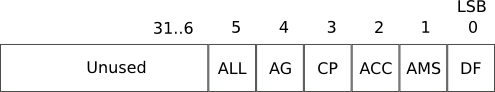
\includegraphics[width=4in]{figure/mobilec_threads_bitfields.png} 
  
  with the following acronyms:
    \begin{itemize}
      \item LSB: Least SignificantBit
      \item DF: Directory Facilitator
      \item AMS: Agent Management System
      \item ACC: Agent Communication Channel
      \item CP: Command Prompt
      \item AG: Agent Threads
    \end{itemize}
    A value of ``1'' in a bitfield tells Mobile-C to enable a particular thread,
    and a value of ``0'' informs Mobile-C not to activate that thread upon
    startup. A set of enumerations are defined in libmc.h that define the macros 
    \texttt{MC\_THREAD\_DF, MC\_THREAD\_AMS}, \texttt{MC\_THREAD\_ACC, MC\_THREAD\_CP, MC\_THREAD\_AGENT},
    each representing the bit position of each thread. There is also a 
    special macro, \texttt{MC\_THREAD\_ALL}, which represents the total number of 
    types of threads in a Mobile-C agency. For instance, to disable
    the command prompt thread, the following code may be used:
    \begin{verbatim}
    options.threads &= ~(1 << MC_OPTIONS_CP);
    \end{verbatim}
    where \texttt{options} is a struct of type \texttt{MCAgencyOptions\_t}.

    Helper functions \texttt{MC\_SetThreadOn(), MC\_SetThreadsAllOn(),
    MC\_SetThreadOff(), MC\_SetThreadsAllOff()} are also provided to modify the
    threads to start. Please consult their repsective documentation pages for
    more information.

  \item \texttt{int default\_agent\_status;} : This is the default agent status
  to assign to all incoming agents. Valid agent status values are found in
  \texttt{libmc.h} under the enumeration \texttt{MC\_AgentStatus\_e}. Possible
  values are:
    \begin{itemize}
    \item \texttt{MC\_WAIT\_CH} : This denotes that the agent is waiting for the
    next available Ch interpereter so that it may execute. This is the default
    setting for all incoming agents.
    \item \texttt{MC\_WAIT\_MESSGSEND} : This agent status indicates that the
    agent has finished its local task, but still has more remote tasks remaining.
    An agent with this status is waiting to be handled by the ACC so that it may
    migrate to the location of its next task.
    \item \texttt{MC\_AGENT\_ACTIVE} : This indicates that the agent is currently
    executing.
    \item \texttt{MC\_AGENT\_NEUTRAL} : This indicates that the agent is not
    executing, but is also not waiting for service. The agent simply persists 
    in the agency. This option is also a popular default alternative to
    \texttt{MC\_WAIT\_CH} since incoming agents are not executed upon arrival.
    \item \texttt{MC\_AGENT\_FINISHED} : This agent status indicates that the
    agent has finished all of its tasks and is awaiting to be purged from the
    agency.
    \end{itemize}
  \item \texttt{int modified;} : This member field is unused.
  \item \texttt{int enable\_security;} : This indicates that the Mobile-C agency
  should enable the Mobile-C security processes. This member is off by default.
  \item \texttt{unsigned char passphrase[32]} : This is a character string a
  passphrase to decrypt the agency's private key. For more details about the
  Mobile-C security process, please refer to Chapter \ref{chap:Security}.
  \item \texttt{int stack\_size[MC\_THREAD\_ALL];} : (Unix only) This array of integers holds
  the stack size to allocate for each thread. For example, if the programmer
  knows in advance that all agents the agency will receive will be small, the
  programmer may limit the stack size of each agent thread to one kilobyte with
  the following line:
  \begin{verbatim}
  options.stack_size[MC_THREAD_AGENT] = 1024;
  \end{verbatim}
  Care should be taken when modifying stack sizes as it may cause instability
  in the system. 
  \item \texttt{char *known\_host\_filename;} : (Optional) This should point to
  a filename containing host names of known and trusted hosts. This file is only
  used if Mobile-C security is enabled.
  \item \texttt{char *priv\_key\_filename;} : (Optional) This should point to a
  string containing the filename of the agency's private key file. This is only
  used if Mobile-C security is enabled.
  \item \texttt{ChOptions\_t* ch\_options;} : This may be used to modify Ch 
  options for agency interpreters. Please refer to the Embedded Ch documentation
  for more information about \texttt{ChOptions\_t}.
\end{itemize}

\noindent
{\bf Example: Starting an agency with default options}\\
\noindent
{\footnotesize\verbatiminput{../demos/getting_started/hello_world/server.c}}

{\bf Example: Starting an agency with no command prompt}\\
\noindent
{\footnotesize\verbatiminput{../demos/FIPA_compliant_ACL_messages/fipa_test/client.c}}

\noindent
{\bf See Also}\\
MC\_End()

%\CPlot::\DataThreeD(), \CPlot::\DataFile(), \CPlot::\Plotting(), \plotxy().\\

\pagebreak
\rhead{\bf MC\_InitializeAgencyOptions()}
\noindent
\vspace{5pt}
\rule{6.5in}{0.015in}
\noindent
\phantomsection
{\LARGE \bf MC\_InitializeAgencyOptions()\index{MC\_InitializeAgencyOptions()}}\\
\addcontentsline{toc}{section}{MC\_InitializeAgencyOptions()}
\label{api:MC_InitializeAgencyOptions()}

\noindent
{\bf Synopsis}\\
{\bf \#include $<$libmc.h$>$}\\
{\bf int MC\_InitializeAgencyOptions}({\bf struct MCAgencyOptions\_s* } options);\\

\noindent
{\bf Purpose}\\
Initialize the agency options structure to default values. \\

\noindent
{\bf Return Value}\\
The function returns 0 on success and non-zero otherwise.\\

\noindent
{\bf Parameters}
\vspace{-0.1in}
\begin{description}
\item
\begin{tabular}{p{10 mm}p{145 mm}} 
$options$ & An uninitialized reference to a \texttt{struct MCAgencyOptions\_s} type variable.
\end{tabular}
\end{description}

\noindent
{\bf Description}\\
This function fills the agency options struct with default values. This
function will overwrite any values that have already been set in the
struct. \\

\noindent
{\bf Example}\\
\noindent
{\footnotesize\verbatiminput{../demos/miscellaneous/mc_sample_app/mc_sample_app.c}}

\noindent
{\bf See Also}\\
MC\_Initialize().

%\CPlot::\DataThreeD(), \CPlot::\DataFile(), \CPlot::\Plotting(), \plotxy().\\

\pagebreak
\rhead{\bf MC\_LoadAgentFromFile()}
\noindent
\vspace{5pt}
\rule{6.5in}{0.015in}
\noindent
\phantomsection
{\LARGE \bf MC\_LoadAgentFromFile()\index{MC\_LoadAgentFromFile()}}\\
\addcontentsline{toc}{section}{MC\_LoadAgentFromFile()}
\label{api:MC_LoadAgentFromFile()}

\noindent
{\bf Synopsis}\\
{\bf \#include $<$libmc.h$>$}\\
{\bf int MC\_LoadAgentFromFile}({\bf MCAgency\_t} $agency$, {\bf const char*} $filename$);\\

\noindent
{\bf Purpose}\\
Add a mobile agent into a local agency from an XML file.\\

\noindent
{\bf Return Value}\\
The function returns 0 on success and non-zero otherwise.\\

\noindent
{\bf Parameters}
\vspace{-0.1in}
\begin{description}
\item
\begin{tabular}{p{10 mm}p{145 mm}} 
$agency$ & An initialized agency handle to add an agent to.\\
$filename$ & An xml file containing a MobileC mobile agent.
\end{tabular}
\end{description}

\noindent
{\bf Description}\\
This function adds a mobile agent to an agency. The agent is loaded from 
an xml file referenced by the \texttt{filename} function argument. \\

\noindent
{\bf Example}\\
\noindent
{\footnotesize\verbatiminput{../demos/communication_with_other_FIPA_compliant_agents/mc_to_jade_example/client.c}}

\noindent
{\bf See Also}\\

%\CPlot::\DataThreeD(), \CPlot::\DataFile(), \CPlot::\Plotting(), \plotxy().\\

\pagebreak
\rhead{\bf MC\_MainLoop()}
\noindent
\vspace{5pt}
\rule{6.5in}{0.015in}
\noindent
{\LARGE \bf MC\_MainLoop()\index{MC\_MainLoop()}}\\
\phantomsection
\addcontentsline{toc}{section}{MC\_MainLoop()}

\noindent
{\bf Synopsis}\\
{\bf \#include $<$libmc.h$>$}\\
{\bf int MC\_MainLoop}({\bf MCAgency\_t} $agency$);\\

\noindent
{\bf Purpose}\\
Cause the calling thread to wait indefinitely on an agency.\\

\noindent
{\bf Return Value}\\
If the Mobile-C agency is terminated safely from another 
thread or agent, the function will return 0. Otherwise, the function will
return a non-zero error code. \\

\noindent
{\bf Parameters}
\vspace{-0.1in}
\begin{description}
\item               
\begin{tabular}{p{10 mm}p{145 mm}}
$agency$ & A handle associated with a running agency. 
\end{tabular}
\end{description}

\noindent
{\bf Description}\\
This function will block the calling thread until another thread or agent
calls the function \texttt{MC\_End()} or \texttt{mc\_End()}, respectively.
This function will also stop blocking if the \texttt{quit} command is issued
from the Mobile-C command prompt.
It must be run on a handle that is attached to an agency that has already 
been started with the function \texttt{MC\_Initialize()}. Also note that 
it is not necessary to call this function to start a valid Mobile-C
agency. All agency threads and services are started upon calling
\texttt{MC\_Initialize()}, and \texttt{MC\_MainLoop()} is generally
only used to prevent the main thread from exiting.\\

\noindent
{\bf Example}\\
\noindent
{\footnotesize\verbatiminput{../demos/getting_started/hello_world/server.c}}

\noindent
{\bf See Also}\\

%\CPlot::\DataThreeD(), \CPlot::\DataFile(), \CPlot::\Plotting(), \plotxy().\\

\pagebreak
\rhead{\bf MC\_MigrateAgent()}
\noindent
\vspace{5pt}
\rule{6.5in}{0.015in}
\noindent
\phantomsection
{\LARGE \bf MC\_MigrateAgent()\index{MC\_MigrateAgent()}}\\
\addcontentsline{toc}{section}{MC\_MigrateAgent()}
\label{api:MC_MigrateAgent()}

\noindent
{\bf Synopsis}\\
{\bf \#include $<$libmc.h$>$}\\
{\bf int MC\_MigrateAgent}({\bf MCAgent\_t} $agent$, {\bf const char*} $hostname$, {\bf int} $port$);\\

\noindent
{\bf Purpose}\\
Instructs an agent to migrate to another host.\\

\noindent
{\bf Return Value}\\
The function returns 0 on success and non-zero otherwise.\\

\noindent
{\bf Parameters}
\vspace{-0.1in}
\begin{description}
\item
\begin{tabular}{p{15 mm}p{145 mm}} 
$agent$ & An initialized mobile agent. \\
$hostname$ & The new host to migrate to. \\
$port$ & The port on the new host to migrate to. \\
\end{tabular}
\end{description}

\noindent
{\bf Description}\\
This function instructs an agent to migrate to a new host. The task of the
agent is not incremented. The agent will executed whatever task it was
currently on when this function was invoked on the new host. Note that this
function only prepends a task to the agents task list. The agent still needs
to finish before the migration step occurs.\\

\noindent
{\bf Example}\\

\noindent
{\bf See Also}\\
mc\_MigrateAgent()

%\CPlot::\DataThreeD(), \CPlot::\DataFile(), \CPlot::\Plotting(), \plotxy().\\

\pagebreak
\rhead{\bf MC\_MutexLock()}
\noindent
\vspace{5pt}
\rule{6.5in}{0.015in}
\noindent
\phantomsection
{\LARGE \bf MC\_MutexLock()\index{MC\_MutexLock()}}\\
\addcontentsline{toc}{section}{MC\_MutexLock()}
\label{api:MC_MutexLock()}

\noindent
{\bf Synopsis}\\
{\bf \#include $<$libmc.h$>$}\\
{\bf int MC\_MutexLock}({\bf MCAgency\_t} agency, {\bf int} $id$);\\

\noindent
{\bf Purpose}\\
This function locks a previously initialized Mobile-C synchronization variable 
as a mutex. 
If the mutex is already locked, the function blocks until it is
unlocked before locking the mutex and continuing. \\

\noindent
{\bf Return Value}\\
This function returns 0 on success, or non-zero if the id could not be found. \\

\noindent
{\bf Parameters}
\vspace{-0.1pt}
\begin{description}
\item
\begin{tabular}{p{10 mm}p{145 mm}} 
$agency$ & The agency in which to find the synchronization variable to lock.\\
$id$ & The id of the synchronization variable to lock. 
\end{tabular}
\end{description}

\noindent
{\bf Description}\\
This function locks the mutex part of a Mobile-C synchronization variable. 
While this is primarily used to guard a shared resource, the behaviour is 
similar to the standard POSIX mutex locking. 
Note that although a MobileC synchronization variable may assume the role of a 
mutex, condition variable, or semaphore, once a Mobile-C synchronization 
variable is used as a mutex, it should not be used as anything else for the 
rest of its life cycle.\\ 

\noindent
{\bf Example}\\
Please see Program \vref{prog:binary_sync_example_server} in 
Chapter \ref{chap:synchronization}.\\

\noindent

\noindent
{\bf See Also}\\
MC\_MutexUnlock(), MC\_SyncInit(), MC\_SyncDelete().\\

%\CPlot::\DataThreeD(), \CPlot::\DataFile(), \CPlot::\Plotting(), \plotxy().\\

\pagebreak
\rhead{\bf MC\_MutexUnlock()}
\noindent
\vspace{5pt}
\rule{6.5in}{0.015in}
\noindent
\phantomsection
{\LARGE \bf MC\_MutexUnlock()\index{MC\_MutexUnlock()}}\\
\addcontentsline{toc}{section}{MC\_MutexUnlock()}

\noindent
{\bf Synopsis}\\
{\bf \#include $<$libmc.h$>$}\\
{\bf int MC\_MutexUnlock}({\bf MCAgency\_t} agency, {\bf int} $id$);\\

\noindent
{\bf Purpose}\\
This function unlocks a locked Mobile-C synchronization variable.\\

\noindent
{\bf Return Value}\\
This function returns 0 on success, or non-zero if the id could not be found.\\

\noindent
{\bf Parameters}
\vspace{-0.1pt}
\begin{description}
\item
\begin{tabular}{p{10 mm}p{145 mm}} 
$agency$ & The agency in which to find the synchronization variable to lock.\\
$id$ & The id of the synchronization variable to lock. 
\end{tabular}
\end{description}

\noindent
{\bf Description}\\
This function unlocks a Mobile-C synchronization variable that was previously
locked as a mutex. 
If the mutex is not locked while calling this function, undefined behaviour 
results.
Note that although a Mobile-C may act as a mutex, condition variable, or 
semaphore, once it has been locked and/or unlocked as a mutex, it should only 
be used as a mutex for the remainder of it's life cycle or unexpected 
behaviour may result.\\

\noindent
{\bf Example}\\
Please see Program \vref{prog:binary_sync_example_server} in 
Chapter \ref{chap:synchronization}.\\
\noindent
%Compare with output for examples in \CPlot::\Arrow(), \CPlot::\AutoScale(),
%\CPlot::\DisplayTime(), \CPlot::\Label(), \CPlot::\TicsLabel(), 
%\CPlot::\Margins(), \CPlot::\BoundingBoxOffsets(), \CPlot::\TicsDirection(),\linebreak
%\CPlot::\TicsFormat(), and \CPlot::\Title().
%{\footnotesize\verbatiminput{template/example/Data2D.ch}}

\noindent
{\bf See Also}\\
MC\_MutexLock(), MC\_SyncInit(), MC\_SyncDelete().\\

%\CPlot::\DataThreeD(), \CPlot::\DataFile(), \CPlot::\Plotting(), \plotxy().\\

\pagebreak
\rhead{\bf MC\_PrintAgentCode()}
\noindent
\vspace{5pt}
\rule{6.5in}{0.015in}
\noindent
{\LARGE \bf MC\_PrintAgentCode()\index{MC\_PrintAgentCode()}}\\
\phantomsection
\addcontentsline{toc}{section}{MC\_PrintAgentCode()}

\noindent
{\bf Synopsis}\\
{\bf \#include $<$libmc.h$>$}\\
{\bf int MC\_PrintAgentCode}({\bf MCAgent\_t} $agent$);\\

\noindent
{\bf Purpose}\\
Print a mobile agent code for inspection.\\

\noindent
{\bf Return Value}\\
The function returns 0 on success and non-zero otherwise.\\

\noindent
{\bf Parameters}
\vspace{-0.1in}
\begin{description}
\item               
\begin{tabular}{p{10 mm}p{145 mm}}
$agent$ & The mobile agent from which to print the code.
\end{tabular}
\end{description}

\noindent
{\bf Description}\\
This function prints the mobile agent code to the standard output.\\

\noindent
{\bf Example}\\
\noindent
%Compare with output for examples in \CPlot::\Arrow(), \CPlot::\AutoScale(),
%\CPlot::\DisplayTime(), \CPlot::\Label(), \CPlot::\TicsLabel(), 
%\CPlot::\Margins(), \CPlot::\BoundingBoxOffsets(), \CPlot::\TicsDirection(),\linebreak
%\CPlot::\TicsFormat(), and \CPlot::\Title().
%{\footnotesize\verbatiminput{template/example/Data2D.ch}}

\noindent
{\bf See Also}\\

%\CPlot::\DataThreeD(), \CPlot::\DataFile(), \CPlot::\Plotting(), \plotxy().\\

\pagebreak
\rhead{\bf MC\_RegisterService()}
\noindent
\vspace{5pt}
\rule{6.5in}{0.015in}
\noindent
\phantomsection
{\LARGE \bf MC\_RegisterService()\index{MC\_RegisterService()}}\\
\addcontentsline{toc}{section}{MC\_RegisterService()}
\label{api:MC_RegisterService()}

\noindent
{\bf Synopsis}\\
{\bf \#include $<$libmc.h$>$}\\
{\bf int MC\_RegisterService}({\bf MCAgency\_t} $agency$, {\bf MCAgent\_t} $agent$, {\bf int} agentID, {\bf const char} agentName, {\bf char**} serviceNames, {\bf int} numServices);\\

\noindent
{\bf Purpose}\\
Registers an agent service with an agency Directory Facilitator.\\

\noindent
{\bf Return Value}\\
The function returns 0 on success and non-zero otherwise.\\

\noindent
{\bf Parameters}
\vspace{-0.1in}
\begin{description}
\item
\begin{tabular}{p{23 mm}p{145 mm}} 
$agency$ & An initialized agency handle to add an agent to.\\
$agent$ & (Optional) An initialized mobile agent. \\
$agentID$ & (Optional) An agent id. \\
$agentName$ & (Optional) An agent name. \\
$serviceNames$ & A list of descriptive names for agent services. \\
$numServices$ & The number of services listed in the previous argument.
\end{tabular}
\end{description}

\noindent
{\bf Description}\\
This function is used to register agent services with an agency. Among
the optional arguments, either a valid agent must be supplied, or both
an agent ID and an agent name. Thus, services may be registered to an
agent which has not yet arrived at an agency by specifying the ID and name
of the agent.\\

\noindent
{\bf Example}\\
\noindent
{\footnotesize\verbatiminput{../demos/agent_space_functionality/mc_df_example/agent1.xml}}

\noindent
{\bf See Also}\\
mc\_RegisterService(), MC\_DeregisterService().

%\CPlot::\DataThreeD(), \CPlot::\DataFile(), \CPlot::\Plotting(), \plotxy().\\

\pagebreak
\rhead{\bf MC\_ResetSignal()}
\noindent
\vspace{5pt}
\rule{6.5in}{0.015in}
\noindent
{\LARGE \bf MC\_ResetSignal()\index{MC\_ResetSignal()}}\\
\phantomsection
\addcontentsline{toc}{section}{MC\_ResetSignal()}

\noindent
{\bf Synopsis}\\
{\bf \#include $<$libmc.h$>$}\\
{\bf int MC\_ResetSignal}({\bf MCAgency\_t} $agency$);\\

\noindent
{\bf Purpose}\\
This function is used to reset the Mobile-C signalling system. 
It is intended to be used after returning from a call to function 
{\bf MC\_WaitSignal()}.\\

\noindent
{\bf Return Value}\\
This function returns 0 on success and non-zero otherwise.\\

\noindent
{\bf Parameters}
\vspace{-0.1in}
\begin{description}
\item               
\begin{tabular}{p{10 mm}p{145 mm}}
$agency$ & A handle to a running agency.
\end{tabular}
\end{description}

\noindent
{\bf Description}\\
This function is used to reset the Mobile-C signalling system. 
System signals are triggered by certain events in the Mobile-C library. 
This includes events such as the arrival of a new message or mobile agent, and 
the departure of a mobile agent, etc. 
If function {\bf MC\_WaitSignal()} is used to listen for one of these events, 
function {\bf MC\_ResetSignal()} must be called in order to allow Mobile-C to 
resume with it's operations.\\

\noindent
{\bf Example}\\
\noindent
{\footnotesize\verbatiminput{../demos/composing_agents/multi_task_example/client.c}}

\noindent
{\bf See Also}\\
MC\_WaitSignal() \\

%\CPlot::\DataThreeD(), \CPlot::\DataFile(), \CPlot::\Plotting(), \plotxy().\\

\pagebreak
\rhead{\bf MC\_ResumeAgency()}
\noindent
\vspace{5pt}
\rule{6.5in}{0.015in}
\noindent
\phantomsection
{\LARGE \bf MC\_ResumeAgency()\index{MC\_ResumeAgency()}}\\
\addcontentsline{toc}{section}{MC\_ResumeAgency()}
\label{api:MC_ResumeAgency()}

\noindent
{\bf Synopsis}\\
{\bf \#include $<$libmc.h$>$}\\
{\bf int MC\_ResumeAgency}({\bf MCAgency\_t} $agency$);\\

\noindent
{\bf Purpose}\\
This function resumes the execution of an agency. \\

\noindent
{\bf Return Value}\\
The function returns 0 on success and non-zero otherwise.\\

\noindent
{\bf Parameters}
\vspace{-0.1in}
\begin{description}
\item
\begin{tabular}{p{10 mm}p{145 mm}} 
$agency$ & An initialized agency handle. 
\end{tabular}
\end{description}

\noindent
{\bf Description}\\
This function resumes the operation of the core threads of the Mobile-C
agency, such as the ACC, AMS, etc., after they have been halted by the 
\texttt{MC\_HaltAgency()} function.\\

\noindent
{\bf Example}\\
\noindent
% FIXME: Need an example here
%{\footnotesize\verbatiminput{../demos/multiple_agency_example/server.c}}

\noindent
{\bf See Also}\\
MC\_HaltAgency().

%\CPlot::\DataThreeD(), \CPlot::\DataFile(), \CPlot::\Plotting(), \plotxy().\\

\pagebreak
\rhead{\bf MC\_RetrieveAgent()}
\noindent
\vspace{5pt}
\rule{6.5in}{0.015in}
\noindent
{\LARGE \bf MC\_RetrieveAgent()\index{MC\_RetrieveAgent()}}\\
\phantomsection
\addcontentsline{toc}{section}{MC\_RetrieveAgent()}

\noindent
{\bf Synopsis}\\
{\bf \#include $<$libmc.h$>$}\\
{\bf MCAgent\_t MC\_RetrieveAgent}({\bf MCAgency\_t} $agency$);\\

\noindent
{\bf Purpose}\\
Retrieve the first neutral mobile agent from a mobile agent list.\\

\noindent
{\bf Return Value}\\
The function returns an {\bf MCAgent\_t} object on success or NULL on failure.\\

\noindent
{\bf Parameters}
\vspace{-0.1in}
\begin{description}
\item               
\begin{tabular}{p{10 mm}p{145 mm}}
$agency$ & An agency handle.\\
\end{tabular}
\end{description}

\noindent
{\bf Description}\\
This function retrieves the first agent with status MC\_AGENT\_NEUTRAL from a 
mobile agent list. 
If there are no mobile agents with this attribute, the return value is NULL.\\

\noindent
{\bf Example}\\
\noindent
%Compare with output for examples in \CPlot::\Arrow(), \CPlot::\AutoScale(),
%\CPlot::\DisplayTime(), \CPlot::\Label(), \CPlot::\TicsLabel(), 
%\CPlot::\Margins(), \CPlot::\BoundingBoxOffsets(), \CPlot::\TicsDirection(),\linebreak
%\CPlot::\TicsFormat(), and \CPlot::\Title().
%{\footnotesize\verbatiminput{template/example/Data2D.ch}}

\noindent
{\bf See Also}\\

%\CPlot::\DataThreeD(), \CPlot::\DataFile(), \CPlot::\Plotting(), \plotxy().\\

\pagebreak
\rhead{\bf MC\_RetrieveAgentCode()}
\noindent
\vspace{5pt}
\rule{6.5in}{0.015in}
\noindent
{\LARGE \bf MC\_RetrieveAgentCode()\index{MC\_RetrieveAgentCode()}}\\
\phantomsection
\addcontentsline{toc}{section}{MC\_RetrieveAgentCode()}
\label{api:MC_RetrieveAgentCode()}

\noindent
{\bf Synopsis}\\
{\bf \#include $<$libmc.h$>$}\\
{\bf char *MC\_RetrieveAgentCode}({\bf MCAgent\_t} $agent$);\\

\noindent
{\bf Purpose}\\
Retrieve a mobile agent code in the form of a character string.\\

\noindent
{\bf Return Value}\\
The function returns an allocated character array on success and NULL on 
failure.\\

\noindent
{\bf Parameters}
\vspace{-0.1in}
\begin{description}
\item               
\begin{tabular}{p{10 mm}p{145 mm}}
$agent$ & The mobile agent from which to retrieve the code.
\end{tabular}
\end{description}

\noindent
{\bf Description}\\
This function retrieves a mobile agent code. 
The return pointer is allocated by 'malloc()' and must be freed by the user.\\

\noindent
{\bf Example}\\
\noindent
{\footnotesize\verbatiminput{../demos/mobilec_c-space_functionality/cspace_misc_examples/server.c}}

\noindent
{\bf See Also}\\

%\CPlot::\DataThreeD(), \CPlot::\DataFile(), \CPlot::\Plotting(), \plotxy().\\

\pagebreak
\rhead{\bf MC\_SearchForService()}
\noindent
\vspace{5pt}
\rule{6.5in}{0.015in}
\noindent
\phantomsection
{\LARGE \bf MC\_SearchForService()\index{MC\_SearchForService()}}\\
\addcontentsline{toc}{section}{MC\_SearchForService()}
\label{api:MC_SearchForService()}

\noindent
{\bf Synopsis}\\
{\bf \#include $<$libmc.h$>$}\\
{\bf int MC\_SearchForService}({\bf MCAgency\_t} $agency$, {\bf char*} SearchString,  {\bf char***} $agentNames$, {\bf char***} serviceNames, {\bf int **} agentIDs,{\bf int*} numResults);\\

\noindent
{\bf Purpose}\\
Searches the Directory Facilitator for a service.\\

\noindent
{\bf Return Value}\\
The function returns 0 on success and non-zero otherwise.\\

\noindent
{\bf Parameters}
\vspace{-0.1in}
\begin{description}
\item
\begin{tabular}{p{23 mm}p{145 mm}} 
$agency$ & An initialized agency handle.\\
$searchString$ & (in) A search substring. All services names registered with the Directory Facilitator with a matching substring will be a hit. \\
$agentNames$ & (out) A newly allocated array of agent names of agents that provide services matching the search string. \\
$serviceNames$ & (out) A newly allocated array of service names matching the search substring. \\
$AgentIDs$ & (out) A newly allocated array of agent IDs of matching agents. \\
$numServices$ & (out) The number of services listed in the previous argument.
\end{tabular}
\end{description}

\noindent
{\bf Description}\\
This function is used to search the Directory Facilitator for a service.
The function will return all services if any part of the service name 
matches the search string. \\

\noindent
{\bf Example}\\
\noindent
{\footnotesize\verbatiminput{../demos/agent_space_functionality/mc_df_example/agent3.xml}}

\noindent
{\bf See Also}\\
MC\_RegisterService(), MC\_DeregisterService().

%\CPlot::\DataThreeD(), \CPlot::\DataFile(), \CPlot::\Plotting(), \plotxy().\\

\pagebreak
\rhead{\bf MC\_SemaphorePost()}
\noindent
\vspace{5pt}
\rule{6.5in}{0.015in}
\noindent
\phantomsection
{\LARGE \bf MC\_SemaphorePost()\index{MC\_SemaphorePost()}}\\
\addcontentsline{toc}{section}{MC\_SemaphorePost()}

\noindent
{\bf Synopsis}\\
{\bf \#include $<$libmc.h$>$}\\
{\bf int MC\_SemaphorePost}({\bf MCAgency\_t} agency, {\bf int} $id$);\\

\noindent
{\bf Purpose}\\
This function unlocks one resource from a Mobile-C semaphore, increasing its
count by one.\\

\noindent
{\bf Return Value}\\
This function returns 0 on success, or non-zero if the id could not be found 
or on a semaphore error.\\

\noindent
{\bf Parameters}
\vspace{-0.1pt}
\begin{description}
\item
\begin{tabular}{p{10 mm}p{145 mm}} 
$agency$ & The agency in which to find the synchronization variable to lock.\\
$id$ & The id of the synchronization variable to lock. 
\end{tabular}
\end{description}

\noindent
{\bf Description}\\
{\bf MC\_SemaphorePost} unlocks a resourse from a previously allocated and 
initialized Mobile-C synchronization variable being used as a semaphore. 
This function may be called multiple times to increase the count of the 
semaphore up to INT\_MAX. 
Note that although a Mobile-C synchronization variable may be used as a mutex, 
condition variable, or semaphore, once it is used as a semaphore, it should 
only be used as a semaphore for the remainder of its life cycle.\\

\noindent
{\bf Example}\\
The MC\_SemaphorePost() function usage is very similar to the other
binary space synchronization functions. Please see Chapter 
\ref{chap:synchronization} on page \pageref{chap:synchronization} 
and the demo at ``demos/agent\_semaphore\_example/'' for
more information.\\
\noindent
%Compare with output for examples in \CPlot::\Arrow(), \CPlot::\AutoScale(),
%\CPlot::\DisplayTime(), \CPlot::\Label(), \CPlot::\TicsLabel(), 
%\CPlot::\Margins(), \CPlot::\BoundingBoxOffsets(), \CPlot::\TicsDirection(),\linebreak
%\CPlot::\TicsFormat(), and \CPlot::\Title().
%{\footnotesize\verbatiminput{template/example/Data2D.ch}}

\noindent
{\bf See Also}\\
MC\_SemaphoreWait(), MC\_SyncInit(), MC\_SyncDelete().\\

%\CPlot::\DataThreeD(), \CPlot::\DataFile(), \CPlot::\Plotting(), \plotxy().\\

\pagebreak
\rhead{\bf MC\_SemaphoreWait()}
\noindent
\vspace{5pt}
\rule{6.5in}{0.015in}
\noindent
\phantomsection
{\LARGE \bf MC\_SemaphoreWait()\index{MC\_SemaphoreWait()}}\\
\addcontentsline{toc}{section}{MC\_SemaphoreWait()}

\noindent
{\bf Synopsis}\\
{\bf \#include $<$libmc.h$>$}\\
{\bf int MC\_SemaphoreWait}({\bf MCAgency\_t} agency, {\bf int} $id$);\\

\noindent
{\bf Purpose}\\
This function allocates one resource from a Mobile-C synchronization semaphore 
variable.\\

\noindent
{\bf Return Value}\\
This function returns 0 on success, or non-zero if the id could not be found.\\

\noindent
{\bf Parameters}
\vspace{-0.1pt}
\begin{description}
\item
\begin{tabular}{p{10 mm}p{145 mm}} 
$agency$ & The agency in which to find the synchronization variable to lock.\\
$id$ & The id of the synchronization variable to lock. 
\end{tabular}
\end{description}

\noindent
{\bf Description}\\
This function allocates one resource from a previously allocated and 
initialized Mobile-C synchronization semaphore. 
If the semaphore resource count is non-zero, the resource is immediately 
allocated. 
If the semaphore resource count is zero, the function blocks until a resource 
is freed before allocating a resource and continuing. 
Note that although a Mobile-C synchronization variable may be used as a mutex, 
condition variable, or semaphore, once it is used as a semaphore, it should 
only be used as a semaphore for the remainder of its life cycle.\\

\noindent
{\bf Example}\\
The MC\_SemaphorePost() function usage is very similar to the other
binary space synchronization functions. Please see Chapter 
\ref{chap:synchronization} on page \pageref{chap:synchronization} for
more information.\\
\noindent
%Compare with output for examples in \CPlot::\Arrow(), \CPlot::\AutoScale(),
%\CPlot::\DisplayTime(), \CPlot::\Label(), \CPlot::\TicsLabel(), 
%\CPlot::\Margins(), \CPlot::\BoundingBoxOffsets(), \CPlot::\TicsDirection(),\linebreak
%\CPlot::\TicsFormat(), and \CPlot::\Title().
%{\footnotesize\verbatiminput{template/example/Data2D.ch}}

\noindent
{\bf See Also}\\
MC\_SemaphorePost(), MC\_SyncInit(), MC\_SyncDelete().\\

%\CPlot::\DataThreeD(), \CPlot::\DataFile(), \CPlot::\Plotting(), \plotxy().\\

\pagebreak
\rhead{\bf MC\_SendAgent()}
\noindent
\vspace{5pt}
\rule{6.5in}{.01in}
\noindent
{\LARGE \bf MC\_SendAgent()\index{MC\_SendAgent()}} \\
\phantomsection
\addcontentsline{toc}{section}{MC\_SendAgent()}

\noindent
{\bf Synopsis}\\
{\bf \#include $<$libmc.h$>$}\\
{\bf int MC\_SendAgent}({\bf MCAgency\_t} $agency$, {\bf char *}$message$);\\

\noindent
{\bf Purpose}\\
Send an ACL mobile agent message to a remote agency.

\noindent
{\bf Return Value}\\
The function returns 0 on success and non-zero otherwise.\\

\noindent
{\bf Parameters}
\vspace{-0.1in}
\begin{description}
\item
\begin{tabular}{p{20 mm}p{135 mm}}
$agency$ & A handle associated with an agency from which to send the ACL 
mobile agent message. A NULL pointer can be used to send the ACL message 
from an unspecified agency.\\ 
$message$ & The ACL mobile agent message to be sent.\\
\end{tabular}
\end{description}

\noindent
{\bf Description}\\
This function is used to send an XML based ACL mobile agent message, which 
is a string, to a remote agency. \\

\noindent
{\bf Example}\\
\noindent
%Compare with output for examples in \CPlot::\Arrow(), \CPlot::\AutoScale(),
%\CPlot::\DisplayTime(), \CPlot::\Label(), \CPlot::\TicsLabel(), 
%\CPlot::\Margins(), \CPlot::\BoundingBoxOffsets(), \CPlot::\TicsDirection(),\linebreak
%\CPlot::\TicsFormat(), and \CPlot::\Title().
%{\footnotesize\verbatiminput{template/example/Data2D.ch}}

\noindent
{\bf See Also}\\

%\CPlot::\DataThreeD(), \CPlot::\DataFile(), \CPlot::\Plotting(), \plotxy().\\

\pagebreak
\rhead{\bf MC\_SendAgentFile()} 
\noindent
\vspace{5pt}
\rule{6.5in}{.01in}
\noindent
{\LARGE \bf MC\_SendAgentFile()\index{MC\_SendAgentFile()}}\\ 
\phantomsection
\addcontentsline{toc}{section}{MC\_SendAgentFile()}
\label{api:MC_SendAgentFile()}

\noindent
{\bf Synopsis}\\
{\bf \#include $<$libmc.h$>$}\\
{\bf int MC\_SendAgentFile}({\bf MCAgency\_t} $agency$, {\bf char *}$filename$);\\

\noindent
{\bf Purpose}\\
Send an ACL mobile agent message saved as a file to a remote agency.

\noindent
{\bf Return Value}\\
The function returns 0 on success and non-zero otherwise.\\

\noindent
{\bf Parameters}
\vspace{-0.1in}
\begin{description}
\item
\begin{tabular}{p{20 mm}p{135 mm}}
$agency$ & A handle associated with an agency from which to send the ACL 
mobile agent message. A NULL pointer can be used to send the ACL message 
from an unspecified agency.\\ 
$filename$ & The ACL mobile agent message file to be sent.\\
\end{tabular}
\end{description}

\noindent
{\bf Description}\\
This function is used to send an XML based ACL mobile agent message, which 
is saved as a file, to a remote agency. \\

\noindent
{\bf Example}\\
\noindent
{\footnotesize\verbatiminput{../demos/getting_started/hello_world/client.c}}

\noindent
{\bf See Also}\\

%\CPlot::\DataThreeD(), \CPlot::\DataFile(), \CPlot::\Plotting(), \plotxy().\\

\pagebreak
\rhead{\bf MC\_SendAgentMigrationMessage()}
\noindent
\vspace{5pt}
\rule{6.5in}{.01in}
\noindent
{\LARGE \bf MC\_SendAgentMigrationMessage()\index{MC\_SendAgentMigrationMessage()}} [Deprecated] \\
\phantomsection
\addcontentsline{toc}{section}{MC\_SendAgentMigrationMessage()}

\noindent
{\bf Synopsis}\\
{\bf \#include $<$libmc.h$>$}\\
{\bf int MC\_SendAgentMigrationMessage}({\bf MCAgency\_t} $agency$, {\bf char *}$message$, {\bf char *}$hostname$, {\bf int} $port$);\\

\noindent
{\bf Purpose}\\
Send an ACL mobile agent message to a remote agency.

Please note that this function is deprecated. Please use the
\texttt{MC\_SendAgent()} function instead.\\

\noindent
{\bf Return Value}\\
The function returns 0 on success and non-zero otherwise.\\

\noindent
{\bf Parameters}
\vspace{-0.1in}
\begin{description}
\item
\begin{tabular}{p{20 mm}p{135 mm}}
$agency$ & A handle associated with an agency from which to send the ACL 
mobile agent message. A NULL pointer can be used to send the ACL message 
from an unspecified agency.\\ 
$message$ & The ACL mobile agent message to be sent.\\
$hostname$ & The hostname of the remote agency. It can be in number-dot 
format or hostname format, i.e., 169.237.104.199 or machine.ucdavis.edu.\\
$port$ & The port number on which the remote agency is listening. 
\end{tabular}
\end{description}

\noindent
{\bf Description}\\
This function is used to send an XML based ACL mobile agent message, which 
is a string, to a remote agency. 
This function can be used without a running local agency.\\

\noindent
{\bf Example}\\
\noindent
%Compare with output for examples in \CPlot::\Arrow(), \CPlot::\AutoScale(),
%\CPlot::\DisplayTime(), \CPlot::\Label(), \CPlot::\TicsLabel(), 
%\CPlot::\Margins(), \CPlot::\BoundingBoxOffsets(), \CPlot::\TicsDirection(),\linebreak
%\CPlot::\TicsFormat(), and \CPlot::\Title().
%{\footnotesize\verbatiminput{template/example/Data2D.ch}}

\noindent
{\bf See Also}\\

%\CPlot::\DataThreeD(), \CPlot::\DataFile(), \CPlot::\Plotting(), \plotxy().\\

\pagebreak
\rhead{\bf MC\_SendAgentMigrationMessageFile()} 
\noindent
\vspace{5pt}
\rule{6.5in}{.01in}
\noindent
{\LARGE \bf MC\_SendAgentMigrationMessageFile()\index{MC\_SendAgentMigrationMessageFile()}} [Deprecated]\\ 
\phantomsection
\addcontentsline{toc}{section}{MC\_SendAgentMigrationMessageFile()}
\label{api:MC_SendAgentMigrationMessageFile()}

\noindent
{\bf Synopsis}\\
{\bf \#include $<$libmc.h$>$}\\
{\bf int MC\_SendAgentMigrationMessageFile}({\bf MCAgency\_t} $agency$, {\bf char *}$filename$, {\bf char *}$hostname$, {\bf int} $port$);\\

\noindent
{\bf Purpose}\\
Send an ACL mobile agent message saved as a file to a remote agency.

Please note that this function is deprecated. Please use the
\texttt{MC\_SendAgentFile()} function instead.\\

\noindent
{\bf Return Value}\\
The function returns 0 on success and non-zero otherwise.\\

\noindent
{\bf Parameters}
\vspace{-0.1in}
\begin{description}
\item
\begin{tabular}{p{20 mm}p{135 mm}}
$agency$ & A handle associated with an agency from which to send the ACL 
mobile agent message. A NULL pointer can be used to send the ACL message 
from an unspecified agency.\\ 
$filename$ & The ACL mobile agent message file to be sent.\\
$hostname$ & The hostname of the remote agency. It can be in number-dot 
format or hostname format, i.e., 169.237.104.199 or machine.ucdavis.edu.\\
$port$ & The port number on which the remote agency is listening. 
\end{tabular}
\end{description}

\noindent
{\bf Description}\\
This function is used to send an XML based ACL mobile agent message, which 
is saved as a file, to a remote agency. 
This function can be used without a running local agency.\\

\noindent
{\bf Example}\\
\noindent
{\footnotesize\verbatiminput{../demos/getting_started/hello_world/client.c}}

\noindent
{\bf See Also}\\

%\CPlot::\DataThreeD(), \CPlot::\DataFile(), \CPlot::\Plotting(), \plotxy().\\

\pagebreak
\rhead{\bf MC\_SendSteerCommand()}
\noindent
\vspace{5pt}
\rule{6.5in}{0.015in}
\noindent
\phantomsection
{\LARGE \bf MC\_SendSteerCommand()\index{MC\_SendSteerCommand()}}\\
\addcontentsline{toc}{section}{MC\_SendSteerCommand()}
\label{api:MC_SendSteerCommand()}

\noindent
{\bf Synopsis}\\
{\bf \#include $<$libmc.h$>$}\\
{\bf int MC\_SendSteerCommand}({\bf MCAgency\_t} $agency$, {\bf enum MC\_SteerCommand\_e} cmd);\\

\noindent
{\bf Purpose}\\
Send a steering command to a Mobile-C computational steering algorithm.\\

\noindent
{\bf Return Value}\\
The function returns 0 on success and non-zero otherwise.\\

\noindent
{\bf Parameters}
\vspace{-0.1in}
\begin{description}
\item
\begin{tabular}{p{10 mm}p{145 mm}} 
$agency$ & An initialized agency handle to add an agent to.\\
$cmd$ & The command to send.
\end{tabular}
\end{description}

\noindent
{\bf Description}\\
This function sends a steering command to a Mobile-C steerable algorithm.

\noindent
{\bf Example}\\
\noindent
{\footnotesize\verbatiminput{../demos/miscellaneous/steer_example/suspend.xml}}

\noindent
{\bf See Also}\\
MC\_Steer(), MC\_SteerControl().

%\CPlot::\DataThreeD(), \CPlot::\DataFile(), \CPlot::\Plotting(), \plotxy().\\

\pagebreak
\rhead{\bf MC\_SetAgentStatus()}
\noindent
\vspace{5pt}
\rule{6.5in}{0.015in}
\noindent
{\LARGE \bf MC\_SetAgentStatus()\index{MC\_SetAgentStatus()}}\\
\phantomsection
\addcontentsline{toc}{section}{MC\_SetAgentStatus()}
\label{api:MC_SetAgentStatus()}

\noindent
{\bf Synopsis}\\
{\bf \#include $<$libmc.h$>$}\\
{\bf int MC\_SetAgentStatus}({\bf MCAgent\_t} $agent$, {\bf int} $status$);\\

\noindent
{\bf Purpose}\\
Set the status of a mobile agent in an agency.\\

\noindent
{\bf Return Value}\\
This function returns 0 on success and non-zero otherwise.\\

\noindent
{\bf Parameters}
\vspace{-0.1in}
\begin{description}
\item               
\begin{tabular}{p{10 mm}p{145 mm}}
$agent$ & The mobile agent whose status is to be assigned.\\
$status$ & An integer representing the status to be assinged to a mobile agent.
\end{tabular}
\end{description}

\noindent
{\bf Description}\\
This function returns an integer of enumerated type
{\texttt enum MC\_AgentStatus\_e}. Details about this enumerated type may be
found in Table \ref{mobilec_macro} on page \pageref{mobilec_macro}.\\

\noindent
{\bf Example}\\
\noindent
{\footnotesize\verbatiminput{../demos/miscellaneous/multiple_agency_example/server.c}}

\noindent
{\bf See Also}\\

%\CPlot::\DataThreeD(), \CPlot::\DataFile(), \CPlot::\Plotting(), \plotxy().\\

\pagebreak
\rhead{\bf MC\_SetDefaultAgentStatus()}
\noindent
\vspace{5pt}
\rule{6.5in}{0.015in}
\noindent
{\LARGE \bf MC\_SetDefaultAgentStatus()\index{MC\_SetDefaultAgentStatus()}}\\
\phantomsection
\addcontentsline{toc}{section}{MC\_SetDefaultAgentStatus()}
\label{api:MC_SetDefaultAgentStatus()}

\noindent
{\bf Synopsis}\\
{\bf \#include $<$libmc.h$>$}\\
{\bf int MC\_SetDefaultAgentStatus}({\bf MCAgency\_t} $agency$, {\bf int} $status$);\\

\noindent
{\bf Purpose}\\
Set the default status of any incoming mobile agents.\\

\noindent
{\bf Return Value}\\
This function returns 0 on success and non-zero otherwise.\\

\noindent
{\bf Parameters}
\vspace{-0.1in}
\begin{description}
\item               
\begin{tabular}{p{10 mm}p{145 mm}}
$agency$ & A handle to a running agency.\\
$status$ & An integer representing the status to be assinged to any incoming 
mobile agents as their default status.
\end{tabular}
\end{description}

\noindent
{\bf Description}\\
This function is used to set the default agent status for all incoming
agents in an agency. By default, every incoming agent is set to status
``MC\_WAIT\_CH'', but that may be changed with this function.
The agent status is an enumerated type ``enum MC\_AgentStatus\_e'', which
may be seen in Table \vref{mobilec_macro}.

\noindent
{\bf Example}\\
\begin{verbatim}
MCAgency_t agency;
agency = MC_Initialize(5050, NULL);
MC_SetDefaultAgentStatus(agency, MC_AGENT_NEUTRAL);

/* etc... */
\end{verbatim}\\
\noindent
%Compare with output for examples in \CPlot::\Arrow(), \CPlot::\AutoScale(),
%\CPlot::\DisplayTime(), \CPlot::\Label(), \CPlot::\TicsLabel(), 
%\CPlot::\Margins(), \CPlot::\BoundingBoxOffsets(), \CPlot::\TicsDirection(),\linebreak
%\CPlot::\TicsFormat(), and \CPlot::\Title().
%{\footnotesize\verbatiminput{template/example/Data2D.ch}}

\noindent
{\bf See Also}\\
MC\_GetAgentStatus()


\pagebreak
\rhead{\bf MC\_SetThreadOff()}
\noindent
\vspace{5pt}
\rule{6.5in}{0.015in}
\noindent
{\LARGE \bf MC\_SetThreadOff()\index{MC\_SetThreadOff()}}\\
\phantomsection
\addcontentsline{toc}{section}{MC\_SetThreadOff()}

\noindent
{\bf Synopsis}\\
{\bf \#include $<$libmc.h$>$}\\
{\bf int MC\_SetThreadOff}({\bf MCAgencyOptions\_t} $*options$, {\bf enum threadIndex\_e} $thread$);\\

\noindent
{\bf Purpose}\\
Set a particular thread to not execute upon Mobile-C initialization.\\

\noindent
{\bf Return Value}\\
This function returns 0 on success and non-zero otherwise. \\

\noindent
{\bf Parameters}
\vspace{-0.1in}
\begin{description}
\item               
\begin{tabular}{p{10 mm}p{145 mm}}
$options$ & An allocated MCAgencyOptions\_t variable.\\
$thread$ & A thread index.
\end{tabular}
\end{description}

\noindent
{\bf Description}\\
This function is used to modify the Mobile-C startup options. 
It is used to disable threads that may otherwise be enabled. 
The threads which may be modified are
\vspace{-0.1in}
\begin{description}
\item               
\begin{tabular}{p{40 mm}p{125 mm}}
MC\_THREAD\_AI : & Agent Initializing Thread - Create agent from incoming messages.\\
MC\_THREAD\_AM : & Agent Managing Thread - Manage active agents.\\
MC\_THREAD\_CL : & Connection Listening Thread - Listen incoming connections.\\
MC\_THREAD\_MR : & Message Receiving Thread - Handle incoming connections and recieve agent messages.\\
MC\_THREAD\_MS : & Message Sending Thread - Handle outgoing connections and send agent messages.\\
MC\_THREAD\_CP : & Command Prompt Thread - Handle an interactive user command prompt.
\end{tabular}
\end{description}

\noindent
{\bf Example}\\
\begin{verbatim}
MCAgencyOptions_t options;
MCAgency_t agency;

/* Turn the listen thread off. We will receive our messages 
   in another method. */
MC_SetThreadOff(&options, MC_THREAD_AI);

/* Start the agency with no listen thread*/
agency = MC_Initialize(5050, &options);

/* etc ... */
\end{verbatim}

\noindent
{\bf See Also}\\
MC\_SetThreadOn()\\
%\CPlot::\DataThreeD(), \CPlot::\DataFile(), \CPlot::\Plotting(), \plotxy().\\


\pagebreak
\rhead{\bf MC\_SetThreadOn()}
\noindent
\vspace{5pt}
\rule{6.5in}{0.015in}
\noindent
{\LARGE \bf MC\_SetThreadOn()\index{MC\_SetThreadOn()}}\\
\phantomsection
\addcontentsline{toc}{section}{MC\_SetThreadOn()}

\noindent
{\bf Synopsis}\\
{\bf \#include $<$libmc.h$>$}\\
{\bf int MC\_SetThreadOn}({\bf MCAgencyOptions\_t} $*options$, {\bf enum threadIndex\_e} $thread$);\\

\noindent
{\bf Purpose}\\
Sets a particular thread to execute upon Mobile C initialization.\\

\noindent
{\bf Return Value}\\
This function returns 0 on success and non-zero otherwise.\\

\noindent
{\bf Parameters}
\vspace{-0.1in}
\begin{description}
\item               
\begin{tabular}{p{10 mm}p{145 mm}}
$options$ & An allocated MCAgencyOptions\_t variable.\\
$thread$ & A thread index.
\end{tabular}
\end{description}

\noindent
{\bf Description}\\
This function is used to modify the Mobile-C startup options. 
It is used to enable threads that may otherwise be disabled. 
The threads which may be modified are
\vspace{-0.1in}
\begin{description}
\item
\begin{tabular}{p{40 mm}p{125 mm}}
MC\_THREAD\_AI : & Agent Initializing Thread - Create agent from incoming messages.\\
MC\_THREAD\_AM : & Agent Managing Thread - Manage active agents.\\
MC\_THREAD\_CL : & Connection Listening Thread - Listen incoming connections.\\
MC\_THREAD\_MR : & Message Receiving Thread - Handle incoming connections and recieve agent messages.\\
MC\_THREAD\_MS : & Message Sending Thread - Handle outgoing connections and send agent messages.\\
MC\_THREAD\_CP : & Command Prompt Thread - Handle an interactive user command prompt.
\end{tabular}
\end{description}

\noindent
{\bf Example}\\
\noindent
\begin{verbatim}
MCAgencyOptions_t options;
MCAgency_t agency;

/* Turn the command prompt thread on */
MC_SetThreadOn(&options, MC_THREAD_CP);

/* Start the agency with a command prompt on port 5050 */
agency = MC_Initialize(5050, &options);

/* etc ... */
\end{verbatim}

\noindent
{\bf See Also}\\
MC\_SetThreadOff()\\
%\CPlot::\DataThreeD(), \CPlot::\DataFile(), \CPlot::\Plotting(), \plotxy().\\


\pagebreak
\rhead{\bf MC\_Steer()}
\noindent
\vspace{5pt}
\rule{6.5in}{0.015in}
\noindent
\phantomsection
{\LARGE \bf MC\_Steer()\index{MC\_Steer()}}\\
\addcontentsline{toc}{section}{MC\_Steer()}

\noindent
{\bf Synopsis}\\
{\bf \#include $<$libmc.h$>$}\\
{\bf int MC\_Steer}({\bf MCAgency\_t} attr, {\bf int} (*funcptr)({\bf void*} data), {\bf void*} arg);\\

\noindent
{\bf Purpose}\\
The MC\_Steer function initialized and runs a function containing an algorithm. 
The function enables the steering functionality of the algorithm so that it may accept 
command during runtime to change the execution of the algorithm. 
For more information, please see the example and the demo located in the 
demos/steer\_example/ directory.\\ 

\noindent
{\bf Return Value}\\
The function returns 0 on success, or a non-zero error code on failure. \\

\noindent
{\bf Description}\\
The {\bf MC\_Steer} function is designed execute an algorithm in a fashion which enables
that algorithm to be steered or modified on-the-fly during runtime. See the demo and
the example for more details. \\

\noindent
{\bf Example}\\
\noindent
{\footnotesize \verbatiminput{../demos/miscellaneous/steer_example/server.c}}
%Compare with output for examples in \CPlot::\Arrow(), \CPlot::\AutoScale(),
%\CPlot::\DisplayTime(), \CPlot::\Label(), \CPlot::\TicsLabel(), 
%\CPlot::\Margins(), \CPlot::\BoundingBoxOffsets(), \CPlot::\TicsDirection(),\linebreak
%\CPlot::\TicsFormat(), and \CPlot::\Title().
%{\footnotesize\verbatiminput{template/example/Data2D.ch}}

\noindent
{\bf See Also}\\
MC\_SteerControl()

%\CPlot::\DataThreeD(), \CPlot::\DataFile(), \CPlot::\Plotting(), \plotxy().\\

\pagebreak
\rhead{\bf MC\_SteerControl()}
\noindent
\vspace{5pt}
\rule{6.5in}{0.015in}
\noindent
\phantomsection
{\LARGE \bf MC\_SteerControl()\index{MC\_SteerControl()}}\\
\addcontentsline{toc}{section}{MC\_SteerControl()}

\noindent
{\bf Synopsis}\\
{\bf \#include $<$libmc.h$>$}\\
{\bf int MC\_SteerControl}({\bf void});\\

\noindent
{\bf Purpose}\\
This function is used to enable Mobile-C as a steerable computational
platform. See the example following for more information, as well
as the demo provided in the directory demos/steer\_example.\\

\noindent
{\bf Return Value}\\
This function returns the current steer command. The command is of type
{\bf enum MC\_Steer\_Command\_e}. This enumerated type contains the following 
definitions:\\
\begin{tabular}{p{55 mm}p{120 mm}}
MC\_RUN & Continue the algorithm. \\
MC\_SUSPEND & Pause the algorithm. \\
MC\_RESTART & Restart the algorithm from the beginning. \\
MC\_STOP & Stop the algorithm.
\end{tabular}\\

\noindent
{\bf Description}\\
{\bf MC\_SteerControl} controls the execution of an algorithm in binary space. 
This function is meant to retrieve the current requested command for the algorithm,
but it is up to the algorithm implementation to actually implement these
behaviours. See the example and the demo for more details.\\ \noindent
{\bf Example}\\
\noindent
{\footnotesize \verbatiminput{../demos/miscellaneous/steer_example/server.c}}
%Compare with output for examples in \CPlot::\Arrow(), \CPlot::\AutoScale(),
%\CPlot::\DisplayTime(), \CPlot::\Label(), \CPlot::\TicsLabel(), 
%\CPlot::\Margins(), \CPlot::\BoundingBoxOffsets(), \CPlot::\TicsDirection(),\linebreak
%\CPlot::\TicsFormat(), and \CPlot::\Title().
%{\footnotesize\verbatiminput{template/example/Data2D.ch}}

\noindent
{\bf See Also}\\
MC\_Steer()

%\CPlot::\DataThreeD(), \CPlot::\DataFile(), \CPlot::\Plotting(), \plotxy().\\

\pagebreak
\rhead{\bf MC\_SyncDelete()}
\noindent
\vspace{5pt}
\rule{6.5in}{0.015in}
\noindent
\phantomsection
{\LARGE \bf MC\_SyncDelete()\index{MC\_SyncDelete()}}\\
\addcontentsline{toc}{section}{MC\_SyncDelete()}
\label{api:MC_SyncDelete()}

\noindent
{\bf Synopsis}\\
{\bf \#include $<$libmc.h$>$}\\
{\bf int MC\_SyncDelete}({\bf int} $id$);\\

\noindent
{\bf Purpose}\\
Delete a previously initialized synchronization variable.\\

\noindent
{\bf Return Value}\\
This function returns 0 on success and nonzero otherwise.\\

\noindent
{\bf Parameters}
\vspace{-0.1in}
\begin{description}
\item
\begin{tabular}{p{10 mm}p{145 mm}} 
$id$ & The id of the condition variable to delete.
\end{tabular}
\end{description}

\noindent
{\bf Description}\\
This function is used to delete and deallocate a previously initialized 
Mobile-C synchronization variable.\\

\noindent
{\bf Example}\\
\noindent
Please see Chapter \ref{chap:synchronization} on synchronization on page
\pageref{chap:synchronization} for more details about using this function.\\

\noindent
{\bf See Also}\\
MC\_SyncInit().\\

%\CPlot::\DataThreeD(), \CPlot::\DataFile(), \CPlot::\Plotting(), \plotxy().\\

\pagebreak
\rhead{\bf MC\_SyncInit()}
\noindent
\vspace{5pt}
\rule{6.5in}{0.015in}
\noindent
\phantomsection
{\LARGE \bf MC\_SyncInit()\index{MC\_SyncInit()}}\\
\addcontentsline{toc}{section}{MC\_SyncInit()}

\noindent
{\bf Synopsis}\\
{\bf \#include $<$libmc.h$>$}\\
{\bf int MC\_SyncInit}({\bf MCAgency\_t} $agency$, {\bf int} $id$);\\

\noindent
{\bf Purpose}\\
Initialize a new synchronization variable.\\

\noindent
{\bf Return Value}\\
This function returns the allocated id of the synchronization variable. Note 
that the allocated id may not necessarily be the same as the requested
id. See the description below for more details.\\

\noindent
{\bf Parameters}
\vspace{-0.1in}
\begin{description}
\item
\begin{tabular}{p{10 mm}p{145 mm}}
$agency$ & The agency in which the new synchronization variable should be 
initialized.\\
$id$ & A requested synchronization variable id. A random id will be assigned 
if the value passed is 0 or if there is a conflicting id.
\end{tabular}
\end{description}

\noindent
{\bf Description}\\
This function initializes a generic Mobile-C synchonization node for use
by agents and the agency. 
Each node contains a mutex, a condition variable, and a semaphore. 
Upon initialization, each variable is initialized to default values: 
The mutex is unlocked and the semaphore has a value of zero.
Each node may be used as a mutex, condition variable, or semaphore. 
Though it is possible to use multiple synchronization variables in a single 
node, this is discouraged as it may lead to unpredictable results. 

Each synchronization variable created by this function is effectively global
across the agency and therefore must have a unique identifying number. If
this function is called requesting an id that is already registered,
the function will automatically ignore the requested value and allocate
a synchronization variable with a randomly generated id.\\

\noindent
{\bf Example}\\
\noindent
Please see Chapter \ref{chap:synchronization} on synchronization on page
\pageref{chap:synchronization} for more details about using this function.\\

\noindent
{\bf See Also}\\
MC\_CondSignal(), MC\_CondWait(), MC\_MutexLock(), MC\_MutexUnlock(), MC\_SemaphorePost(),\\ MC\_SemaphoreWait(), MC\_SyncDelete().\\

%\CPlot::\DataThreeD(), \CPlot::\DataFile(), \CPlot::\Plotting(), \plotxy().\\

\pagebreak
\rhead{\bf MC\_TerminateAgent()}
\noindent
\vspace{5pt}
\rule{6.5in}{0.015in}
\noindent
{\LARGE \bf MC\_TerminateAgent()\index{MC\_TerminateAgent()}}\\
\phantomsection
\addcontentsline{toc}{section}{MC\_TerminateAgent()}

\noindent
{\bf Synopsis}\\
{\bf \#include $<$libmc.h$>$}\\
{\bf int MC\_TerminateAgent}({\bf MCAgent\_t} $agent$);\\

\noindent
{\bf Purpose}\\
Terminate the execution of a mobile agent in an agency.\\

\noindent
{\bf Return Value}\\
The function returns 0 on success and an error code on failure.\\

\noindent
{\bf Parameters}
\vspace{-0.1in}
\begin{description}
\item               
\begin{tabular}{p{10 mm}p{145 mm}}
$agent$ & A valid mobile agent. 
\end{tabular}
\end{description}

\noindent
{\bf Description}\\
This function halts a running mobile agent. 
The Ch interpreter is left intact. 
The mobile agent may still reside in the agency in MC\_AGENT\_NEUTRAL mode if 
the mobile agent is tagged as 'persistent', or is terminated and flushed 
otherwise.\\

\noindent
{\bf Example}\\
This function is identical to the agent-space counterpart. Please see the example
listed under mc\_TerminateAgent() on page \pageref{api:mc_TerminateAgent()}.\\
\noindent

\noindent
{\bf See Also}\\

%\CPlot::\DataThreeD(), \CPlot::\DataFile(), \CPlot::\Plotting(), \plotxy().\\

\pagebreak
%\rhead{\bf MC\_Wait()}
\noindent
\vspace{5pt}
\rule{6.5in}{0.015in}
\noindent
{\LARGE \bf MC\_Wait()\index{MC\_Wait()}}\\
\phantomsection
\addcontentsline{toc}{section}{MC\_Wait()}

\noindent
{\bf Synopsis}\\
{\bf \#include $<$libmc.h$>$}\\
{\bf int MC\_Wait}({\bf MCAgency\_t} $agency$);\\

\noindent
{\bf Purpose}\\
Cause the calling thread to wait indefinitely on an agency.\\

\noindent
{\bf Return Value}\\
The function returns 0 on success and non-zero otherwise.\\

\noindent
{\bf Parameters}
\vspace{-0.1in}
\begin{description}
\item               
\begin{tabular}{p{10 mm}p{145 mm}}
$agency$ & A handle associated with a running agency. 
\end{tabular}
\end{description}

\noindent
{\bf Description}\\
This function simply waits for the agency. 
It must be run on a handle that is attached to an agency that has already 
been started with the function {\bf MC\_Initialize()}.\\

\noindent
{\bf Example}\\
\noindent
{\footnotesize\verbatiminput{../demos/getting_started/hello_world/server.c}}

\noindent
{\bf See Also}\\

%\CPlot::\DataThreeD(), \CPlot::\DataFile(), \CPlot::\Plotting(), \plotxy().\\

%\pagebreak
\rhead{\bf MC\_WaitAgent()}
\noindent
\vspace{5pt}
\rule{6.5in}{0.015in}
\noindent
{\LARGE \bf MC\_WaitAgent()\index{MC\_WaitAgent()}}\\
\phantomsection
\addcontentsline{toc}{section}{MC\_WaitAgent()}

\noindent
{\bf Synopsis}\\
{\bf \#include $<$libmc.h$>$}\\
{\bf int MC\_WaitAgent}({\bf MCAgency\_t} $agency$);\\

\noindent
{\bf Purpose}\\
Cause the calling thread to wait until a mobile agent is received.\\

\noindent
{\bf Return Value}\\
The function returns 0 on success and non-zero otherwise.\\

\noindent
{\bf Parameters}
\vspace{-0.1in}
\begin{description}
\item               
\begin{tabular}{p{10 mm}p{145 mm}}
$agency$ & A handle associated with a running agency. 
\end{tabular}
\end{description}

\noindent
{\bf Description}\\
This function waits on an agency and wakes up the addition of a new
mobile agent to the agency.\\

\noindent
{\bf Example}\\
\noindent
%Compare with output for examples in \CPlot::\Arrow(), \CPlot::\AutoScale(),
%\CPlot::\DisplayTime(), \CPlot::\Label(), \CPlot::\TicsLabel(), 
%\CPlot::\Margins(), \CPlot::\BoundingBoxOffsets(), \CPlot::\TicsDirection(),\linebreak
%\CPlot::\TicsFormat(), and \CPlot::\Title().
%{\footnotesize\verbatiminput{template/example/Data2D.ch}}

\noindent
{\bf See Also}\\

%\CPlot::\DataThreeD(), \CPlot::\DataFile(), \CPlot::\Plotting(), \plotxy().\\

\pagebreak
\rhead{\bf MC\_WaitRetrieveAgent()}
\noindent
\vspace{5pt}
\rule{6.5in}{0.015in}
\noindent
{\LARGE \bf MC\_WaitRetrieveAgent()\index{MC\_WaitRetrieveAgent()}}\\
\phantomsection
\addcontentsline{toc}{section}{MC\_WaitRetrieveAgent()}

\noindent
{\bf Synopsis}\\
{\bf \#include $<$libmc.h$>$}\\
{\bf MCAgent\_t MC\_WaitRetrieveAgent}({\bf MCAgency\_t} $agency$);\\

\noindent
{\bf Purpose}\\
Block the calling thread until a mobile agent arrives, and return the mobile 
agent instead of executing it.\\

\noindent
{\bf Return Value}\\
The function returns a mobile agent on success and a NULL on failure.\\

\noindent
{\bf Parameters}
\vspace{-0.1in}
\begin{description}
\item               
\begin{tabular}{p{10 mm}p{145 mm}}
$agency$ & A handle associated with a running agency. 
\end{tabular}
\end{description}

\noindent
{\bf Description}\\
This function waits on an agency and wakes up the addition of a new mobile 
agent to the agency. 
It will then remove the mobile agent from the agency and return it.\\

\noindent
{\bf Example}\\
\noindent
{\footnotesize\verbatiminput{../demos/mobilec_c-space_functionality/cspace_misc_examples/server.c}}

\noindent
{\bf See Also}\\

%\CPlot::\DataThreeD(), \CPlot::\DataFile(), \CPlot::\Plotting(), \plotxy().\\

\pagebreak
\rhead{\bf MC\_WaitSignal()}
\noindent
\vspace{5pt}
\rule{6.5in}{0.015in}
\noindent
{\LARGE \bf MC\_WaitSignal()\index{MC\_WaitSignal()}}\\
\phantomsection
\addcontentsline{toc}{section}{MC\_WaitSignal()}

\noindent
{\bf Synopsis}\\
{\bf \#include $<$libmc.h$>$}\\
{\bf int MC\_WaitSignal}({\bf MCAgency\_t} $agency$, {\bf int} $signals$);\\

\noindent
{\bf Purpose}\\
This function is used to block the execution of a Mobile-C library application 
until the event of a signal.\\

\noindent
{\bf Return Value}\\
This function returns 0 on success and non-zero otherwise.\\

\noindent
{\bf Parameters}
\vspace{-0.1pt}
\begin{description}
\item
\begin{tabular}{p{10 mm}p{145 mm}}
$agency$ & A handle to a running agency.\\
$signals$ & A bitwise-or combination of signals to wait on.
\end{tabular}
\end{description}

\noindent
{\bf Description}\\
This function is used to block the execution of an application using the 
Mobile-C library until a given signal is received as specfied by the 
parameter $signals$. 
Currently implemented signals that may be waited on are:
\vspace{-0.1in}
\begin{description}
\item               
\begin{tabular}{p{50 mm}p{120 mm}}
MC\_RECV\_CONNECTION : & Continue after a connection is initialized.\\
MC\_RECV\_MESSAGE : & Continue after a message is received.\\
MC\_RECV\_AGENT : & Continue after an agent is received.\\
MC\_RECV\_RETURN: & Continue after return data is received.\\
MC\_EXEC\_AGENT : & Continue after an agent is finished executing.\\
MC\_ALL\_SIGNALS : & Continue after any one of the above events occurs. 
\end{tabular}
\end{description}
In order to wait on a custom combination of signals, the bitwise 'or operator' 
may be used to specify combinations of signals.\\ 

\noindent
{\bf Example}\\
\begin{verbatim}
/* More code here. */

/* Now we wait until we receive a message or mobile agent. */
MC_WaitSignal(agency, RECV_MESSAGE | RECV_AGENT);

/* At this point, a message or mobile agent has been received. */

/* Perform operations on the new message or mobile agent here. */

/* Resume the Mobile-C library */
MC_ResetSignal(agency);

/* More code here. */
\end{verbatim}
\noindent
The above piece of code blocks execution until either a RECV\_MESSAGE or a 
RECV\_AGENT event occurs.
The function {\bf MC\_ResetSignal()} must be invoked at some point after 
returning from {\bf MC\_WaitSignal()} in order for Mobile-C to resume normal 
operations.\\
%Compare with output for examples in \CPlot::\Arrow(), \CPlot::\AutoScale(),
%\CPlot::\DisplayTime(), \CPlot::\Label(), \CPlot::\TicsLabel(), 
%\CPlot::\Margins(), \CPlot::\BoundingBoxOffsets(), \CPlot::\TicsDirection(),\linebreak
%\CPlot::\TicsFormat(), and \CPlot::\Title().
%{\footnotesize\verbatiminput{template/example/Data2D.ch}}

\noindent
{\bf See Also}\\
MC\_ResetSignal()\\

%\CPlot::\DataThreeD(), \CPlot::\DataFile(), \CPlot::\Plotting(), \plotxy().\\

\pagebreak


\chapter{Mobile-C API in the C/C++ Script Space \label {appendixb}}
% Mobile-C Library 

%%%%%%%%%%%%%%%%%%%%%%%%%%%%%%%%%%%%%%%%%%%%%%%%%%%%%%%%%%%%%%%%%%%%%%
% Preamble {{{
%\documentclass[11pt]{article}
\documentclass[11pt]{report}
\usepackage{varioref}
\usepackage{times,here,verbatim,fancyheadings,makeidx}
%\usepackage{psfig}
\usepackage[pdftex]{hyperref}
\usepackage{hypcap}
\usepackage{fullpage}
\usepackage{amssymb,amsmath}
\usepackage{graphicx}
\usepackage{program}
\headrulewidth 0.0pt
\hoffset=-0.0625in
%\voffset=0pt
\setlength{\textheight}{9in}
\setlength{\textwidth}{6.5in}
\topmargin=0.05in
\makeindex
% }}} Preamble
%%%%%%%%%%%%%%%%%%%%%%%%%%%%%%%%%%%%%%%%%%%%%%%%%%%%%%%%%%%%%%%%%%%%%%

%%%%%%%%%%%%%%%%%%%%%%%%%%%%%%%%%%%%%%%%%%%%%%%%%%%%%%%%%%%%%%%%%%%%%%
% Title Page {{{
\begin{document}
\thispagestyle{empty}
\begin{center}

\includegraphics[width=1.8in]{figure/mobilec_logo.png}


\vspace{0.5in}
{\Huge\sf\bf Mobile-C} \\
\vspace{0.1in}
{\LARGE\sf\bf -- A Multi-Agent Platform for Mobile C/C++ Agents} \\
\vspace{0.4in}
{\LARGE\sf\bf User's Guide} \\
\vspace{0.4in}
{\LARGE\sf\bf Version 2.1.3} \\
\vspace{1.0in}
{\Large\sf\bf Harry H. Cheng} \\
\vspace{1.0in}
{\large\sf\bf Mobile-C User's Guide version 2.1.3 prepared by:} \\
\vspace{0.2in}
David Ko\\
Harry H. Cheng
\vspace{1in}

\vspace{2.0in}
{\large\sf\bf\today}
%September 20, 2007
\end{center}

%%%%%%%%%%%%%%%%%%%%%%%%%%%%%%%%%%%%%%%%%%%%%%%%%%%%%%%%%%%%%%%%%%%%%%
% Contributors {{{
%\phantomsection
%\addcontentsline{toc}{chapter}{Major contributors}
\pagebreak
\noindent
{\LARGE\sf\bf Major Contributors (in alphabetical order)} \\
{\small
\verbatiminput{../AUTHORS}
}
% }}} Contributors 
%%%%%%%%%%%%%%%%%%%%%%%%%%%%%%%%%%%%%%%%%%%%%%%%%%%%%%%%%%%%%%%%%%%%%%
\pagebreak


%%%%%%%%%%%%%%%%%%%%%%%%%%%%%%%%%%%%%%%%%%%%%%%%%%%%%%%%%%%%%%%%%%%%%%
% Copyright {{{
\thispagestyle{empty}
%\phantomsection
%\addcontentsline{toc}{chapter}{Copyright}
\noindent
{\Large\bf Copyright}\\
\verbatiminput{../Copyright}
% }}} Copyright 
%%%%%%%%%%%%%%%%%%%%%%%%%%%%%%%%%%%%%%%%%%%%%%%%%%%%%%%%%%%%%%%%%%%%%%

\pagebreak
% }}} Title Page
%%%%%%%%%%%%%%%%%%%%%%%%%%%%%%%%%%%%%%%%%%%%%%%%%%%%%%%%%%%%%%%%%%%%%%

%%%%%%%%%%%%%%%%%%%%%%%%%%%%%%%%%%%%%%%%%%%%%%%%%%%%%%%%%%%%%%%%%%%%%%
% Abstract {{{
%\phantomsection
%\addcontentsline{toc}{chapter}{Abstract}
\begin{abstract} 
Mobile-C is an IEEE FIPA (Foundation for Intelligent Physical Agents) standard 
compliant multi-agent platform for supporting C/C++ mobile agents in networked 
intelligent mechatronic and embedded systems. Although it is a general-purpose 
multi-agent platform, Mobile-C is specifically designed for real-time and 
resource constrained applications with interface to hardware. Mobile agents 
are software components that are able to move between different execution 
environments. Mobile agents in a multi-agent system communicate and work 
collaboratively with other agents to achieve a global goal. It allows a 
mechatronic or embedded system to adapt to a dynamically changing environment.

\vspace{1in}
%%%%%%%%%%%%%%%%%%%% begin figure %%%%%%%%%%%%%%%%%%%% 
%\begin{figure}[H]
\centerline{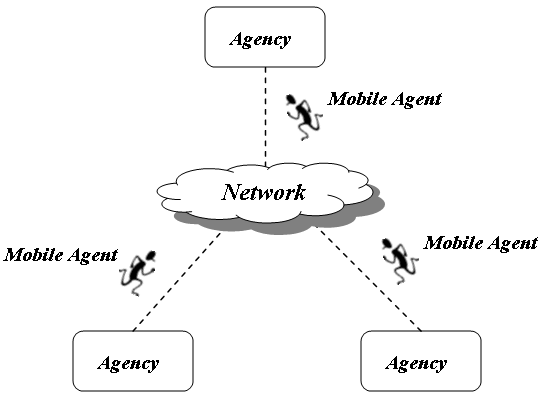
\includegraphics[scale=0.6]{figure/coverfigure}}
%\end{figure}
%%%%%%%%%%%%%%%%%%%% end figure %%%%%%%%%%%%%%%%%%%%%%
\end{abstract}
\pagebreak
% Abstract }}}
%%%%%%%%%%%%%%%%%%%%%%%%%%%%%%%%%%%%%%%%%%%%%%%%%%%%%%%%%%%%%%%%%%%%%%

%%%%%%%%%%%%%%%%%%%%%%%%%%%%%%%%%%%%%%%%%%%%%%%%%%%%%%%%%%%%%%%%%%%%%%
% Table of Contents {{{
\pagenumbering{roman}
\setcounter{page}{1}
\tableofcontents
\pagebreak
% }}} Table of Contents
%%%%%%%%%%%%%%%%%%%%%%%%%%%%%%%%%%%%%%%%%%%%%%%%%%%%%%%%%%%%%%%%%%%%%%

%%%%%%%%%%%%%%%%%%%%%%%%%%%%%%%%%%%%%%%%%%%%%%%%%%%%%%%%%%%%%%%%%%%%%%
% Part 1 {{{
\pagenumbering{arabic}
\setcounter{page}{1}
\pagebreak
% }}} Part 1 
%%%%%%%%%%%%%%%%%%%%%%%%%%%%%%%%%%%%%%%%%%%%%%%%%%%%%%%%%%%%%%%%%%%%%%

%%%%%%%%%%%%%%%%%%%%%%%%%%%%%%%%%%%%%%%%%%%%%%%%%%%%%%%%%%%%%%%%%%%%%%
% Introduction {{{
%\pagenumbering{arabic}
%\setcounter{page}{1}
%\pagestyle{fancy}
\chapter{Introduction}
Parallel and distributed computing~\cite{Kumar}~\cite{Manber} are widely used 
in scientific and engineering fields, especially for time-critical or 
time-consuming tasks.
Parallel computing is typically carried out in dedicated multiprocessors with
a central clock and shared memory.
On the other hand, distributed computing is decentralized parallel
computing, using two or more computers communicating over a network to
accomplish a common objective or task.
It is similar to computer clustering with the main difference being a wide
geographic dispersion of the resources.
In addition to the main difference, the types of hardware, programming 
languages, operating systems and other resources may vary drastically as well 
in distributed computing.

Although the processing speed of networked computers is typically not as fast 
as that of a dedicated parallel computer, networked computers are less
expensive and more broadly available.
Due to the rapid improvement in network hardware and software that makes
distributed computing faster, more broadly available, and easier-to-implement
than before, there are more and more research investigations nowadays 
targeting or exploiting this low-end, decentralized parallel computing.
Meanwhile, as the scale of distributed applications rapidly expands, 
there is an increasing demand for the code mobility.

Agent technology can significantly enhance the design and analysis of 
problem domains under the following three conditions~\cite{Adler}: 
(1) the problem domain is geographically distributed; 
(2) the subsystems exist in a dynamic environment; 
(3) the subsystems need to interact with each other more flexibly. 
Mobile agents are software components that can travel between 
different execution environments~\cite{Fuggetta}. 
Mobile agents can be created dynamically during runtime and dispatched to 
source systems to perform tasks with the most updated code. 
Therefore, the mobility of mobile agents provides distributed 
applications with significant flexibility and adaptability which are both 
essential to satisfy the dynamically changing requirements and conditions in 
a distributed environment.

Most of the mobile agent systems were developed to support only Java mobile 
agents.
Furthermore, many of them are standalone platforms. 
In other words, they were not designed to be embedded in a user application 
to support code mobility.  
Mobile-C~\cite{Chenthesis}~\cite{Chen3}~\cite{Mobile-C}~\cite{mobilec_webpage} 
was originally developed as a standalone, IEEE Foundation for Intelligent 
Physical Agents (FIPA) compliant mobile agent platform with a primary 
intention to fit applications where low-level hardware gets involved, such as 
networked mechatronic and embedded systems. 
Since most of these systems are written in C/C++, Mobile-C uses C/C++ as 
the mobile agent language for easy interfacing with control programs and 
underlying hardware. 
In addition, Mobile-C uses an embeddable C/C++ interpreter -- Ch, originally 
developed by Cheng~\cite{SP1}~\cite{CUJ1}~\cite{Ch}, to support the execution 
of C/C++ mobile agent code. 

In order to provide distributed applications with code mobility, this 
user's guide presents a mobile agent library, the Mobile-C library. 
The Mobile-C library is supported in various operating systems including 
Windows, Unix, and real-time OS.
It has a small footprint to satisfy the small memory requirement for a 
variety of mechatronic and embedded systems. 
This mobile agent library allows Mobile-C to be embedded in a program to 
support C/C++ mobile agents.
The API functions in this library facilitate the development of a multi-agent
system that can easily interface with a variety of hardware devices. 
%\pagebreak
% }}} Introduction
%%%%%%%%%%%%%%%%%%%%%%%%%%%%%%%%%%%%%%%%%%%%%%%%%%%%%%%%%%%%%%%%%%%%%%

%%%%%%%%%%%%%%%%%%%%%%%%%%%%%%%%%%%%%%%%%%%%%%%%%%%%%%%%%%%%%%%%%%%%%%
% Mobile-C Library Installation {{{
\chapter{Mobile-C Library Installation}
This chapter describes the prerequisites to install the Mobile-C library and 
the installation steps for both Unix and Windows operating systems.

%%%%%%%%%%%%%%%%%%%%%%%%%%%%%%%%%%%%%%%%%%%%%%%%%%%%%%%%%%%%%%%%%%%%%%
% SUB: Requirements {{{
\section{Requirements}
This user's guide assumes all necessary software packages are installed
correctly and function. 
The software packages required to successfully install the Mobile-C library 
include:

\noindent
(1) Ch version 6.3.0 or greater: It can be obtained from http://www.softintegration.com

\noindent
(2) Embedded Ch version 6.3.0 or greater: It can be obtained from http://www.softintegration.com

% }}} SUB: Prerequisites 
%%%%%%%%%%%%%%%%%%%%%%%%%%%%%%%%%%%%%%%%%%%%%%%%%%%%%%%%%%%%%%%%%%%%%%

%%%%%%%%%%%%%%%%%%%%%%%%%%%%%%%%%%%%%%%%%%%%%%%%%%%%%%%%%%%%%%%%%%%%%%
% SUB: Installation on Unix {{{
\section{Installation on Unix}

\subsection{Install the Mobile-C library}
The following commands will install the Mobile-C library in the system 
directory for {\bf 32-bit} Unix systems. 
The system directory for Unix systems is usually `/usr/local/lib' or 
  `/usr/lib' depending on your system.

\begin{verbatim}
    cd <MCPACKAGE>/src
    ./configure
    make
    make install
\end{verbatim}

The following commands will install the Mobile-C library in the system 
  directory for {\bf 64-bit} Unix systems. 
The only difference between the above and below commands is that `fPIC' is 
  added into CFLAGS for compilation.

\begin{verbatim}
    cd <MCPACKAGE>/src
    ./configure CFLAGS=-fPIC
    make
    make install
\end{verbatim}

By default, the Mobile-C library created contains both shared and static 
versions, which are `libmc.so.0.0.0' and `libmc.a', respectively.
The header file, libmc.h, used in the C/C++ binary 
space will be placed in the system directory, which is usually 
`usr/local/include' or `/usr/include' depending on your system.
 
Note that these commands will automatically build mxml-2.2.2 and
xyssl-0.7, both of which are packaged with Mobile-C, but will
not install these libraries. The Mobile-C libraries only need
these libraries to compile, but does not need them installed in
order to run.

Also note that the above commands will automatically compile all the included
demos automatically after compiling the Mobile-C library. The demos will
run even if the 'make install' step is omitted.

The `--prefix' option can be used to specify the home directory to 
install the Mobile-C files, as shown in the following commands.

\begin{verbatim}
    cd <MCPACKAGE>/src
    ./configure --prefix=<MCHOME>
    make
    make install
\end{verbatim}

\noindent
\texttt{<MCPACKAGE>} is the directory created by unpacking the Mobile-C compressed 
tar file.
\texttt{<MCHOME>} is the installation directory for the Mobile-C library and 
header file.\\
\noindent
The library files `libmc.so.0.0.0' and `libmc.a' will be installed in 
\texttt{<MCHOME>/lib}, and the header file `libmc.h' will be placed in 
\texttt{<MCHOME>/include}.

% }}} SUB: Installation on Unix
%%%%%%%%%%%%%%%%%%%%%%%%%%%%%%%%%%%%%%%%%%%%%%%%%%%%%%%%%%%%%%%%%%%%%%

%%%%%%%%%%%%%%%%%%%%%%%%%%%%%%%%%%%%%%%%%%%%%%%%%%%%%%%%%%%%%%%%%%%%%%
% SUB: Installation on Windows {{{
\section{Installation on Windows}
\subsection{Building the Mobile-C Library}
The following steps are suggested to build the Mobile-C library.
\begin{enumerate}
\item Ensure that your \texttt{\_chrc} file in your home directory is up to
  date. The \texttt{\_chrc} file may be opened from the ChIDE text editor by
  opening ChIDE, selecting "Options" from the menu, and selecting the "Open
  Local Ch Startup File" menu item. The section in your \texttt{\_chrc} file
  which contains settings about
  your Visual C++ installation must be correct. 
\item Unpack the Mobile-C source code. Ensure that you have write permissions
  for the directory you are unpacking Mobile-C into, or you may encounter 
  compile-time errors. As mentioned in the previous section, we will refer
  to the unpacked directory as \texttt{<MCPACKAGE>}.
\item Open a Ch terminal.
\item Navigate to the \texttt{<MCPACKAGE>} directory in your Ch terminal. For
  example, if you unpacked Mobile-C to the \texttt{C:$\backslash$Mobile-C} directory, type
  \texttt{cd C:$\backslash$Mobile-C} in your Ch terminal.
\item Type the command \texttt{nmake -f makefile.win32} to build the Mobile-C
  library, as well as all of the demos in the \texttt{<MCPACKAGE>/demos/}
  directory.
\end{enumerate}
% }}} SUB: Installation on Windows 
%%%%%%%%%%%%%%%%%%%%%%%%%%%%%%%%%%%%%%%%%%%%%%%%%%%%%%%%%%%%%%%%%%%%%%

%%%%%%%%%%%%%%%%%%%%%%%%%%%%%%%%%%%%%%%%%%%%%%%%%%%%%%%%%%%%%%%%%%%%%%
% SUB: Installation on KoreBot {{{
\section{Installation on KoreBot}

\subsection{Build the Mobile-C library}
A bash script, \textit{build\_korebot}, is used to build the Mobile-C library 
and an executable sample program, \textit{mc\_sample\_app}, for KoreBot board.

Running the script will create a directory called \textit{korebot\_mc} that 
contains \textit{bin}, \textit{include} and \textit{lib} directories.
\textit{bin} directory contains the executable sample program.    
\textit{include} directory contains the header file \textit{libmc.h}.
\textit{lib} directory contains the Mobile-C related static and shared 
libraries.

Two paths, \textit{KOREBOT\_CHHOME} and \textit{KOREBOT\_TOOLCHAINHOME}, 
in the bash script might need to be changed to match the correct 
paths set up in a user's system.
\textit{KOREBOT\_CHHOME} is the directory containing Ch files built for 
KoreBot board.
\textit{KOREBOT\_TOOLCHAINHOME} is the directory containing cross compiler 
related files for KoreBot board. 

Use the following commands to run the bash script.

\begin{verbatim}
    cd <MCPACKAGE>
    ./build_korebot
\end{verbatim}
% }}} SUB: Installation on KoreBot 
%%%%%%%%%%%%%%%%%%%%%%%%%%%%%%%%%%%%%%%%%%%%%%%%%%%%%%%%%%%%%%%%%%%%%%

%%%%%%%%%%%%%%%%%%%%%%%%%%%%%%%%%%%%%%%%%%%%%%%%%%%%%%%%%%%%%%%%%%%%%%
% SUB: Installation on Gumstix {{{
\section{Installation on Gumstix}

\subsection{Build the Mobile-C library}
A bash script, \textit{build\_gumstix}, is used to build the Mobile-C library 
and an executable sample program, \textit{mc\_sample\_app}, for Gumstix 
computer.

Running the script will create a directory called \textit{gumstix\_mc} that 
contains \textit{bin}, \textit{include} and \textit{lib} directories.
\textit{bin} directory contains the executable sample program.    
\textit{include} directory contains the header file \textit{libmc.h}.
\textit{lib} directory contains the Mobile-C related static and shared 
libraries.

Two paths, \textit{GUMSTIX\_CHHOME} and \textit{GUMSTIX\_TOOLCHAINHOME}, 
in the bash script might need to be changed to match the correct 
paths set up in a user's system.
\textit{GUMSTIX\_CHHOME} is the directory containing Ch files built for 
Gumstix computer. By default, it is set to the value \texttt{/usr/local/gumstix\_ch/ch/}.
\textit{GUMSTIX\_TOOLCHAINHOME} is the directory containing cross compiler 
related files for Gumstix computer. By default, it is set to the value \texttt{/usr/local/gumstix-buildroot}.

Use the following commands to run the bash script.

\begin{verbatim}
    cd <MCPACKAGE>
    ./build_gumstix
\end{verbatim}
% }}} SUB: Installation on Gumstix 
%%%%%%%%%%%%%%%%%%%%%%%%%%%%%%%%%%%%%%%%%%%%%%%%%%%%%%%%%%%%%%%%%%%%%%

%%%%%%%%%%%%%%%%%%%%%%%%%%%%%%%%%%%%%%%%%%%%%%%%%%%%%%%%%%%%%%%%%%%%%%
% Installing the Mobile-C Ch Package{{{
\section{Installing the Mobile-C Ch Package}
The Mobile-C Ch Package will be required if agents need to use any of the
Mobile-C FIPA ACL message functions, such as \texttt{mc\_AclSend()} or
\texttt{mc\_AclRetrieve()}. To install the Mobile-C Ch package, please follow
these steps:
\begin{enumerate}
\item From the Mobile-C root directory, run the command: \\
\texttt{ch ./pkgcreate.ch} \\
This will create a directory called ``\texttt{chmobilec}''.
\item From within a Ch shell, run the command: \\
\texttt{sudo pkginstall.ch chmobilec} \\
If you are using Microsoft Windows, you may omit the "\texttt{sudo}" part of the
command which is required on unix-like systems to ensure proper installation
permassions.
\end{enumerate}
% }}} Installing the Mobile-C Security Module
%%%%%%%%%%%%%%%%%%%%%%%%%%%%%%%%%%%%%%%%%%%%%%%%%%%%%%%%%%%%%%%%%%%%%%

\section{Creating your own compilation environment}
If a custom build environment is required, there are several directories which
must be added to the search paths for header files and libraries. There are 
also a variety of system libraries which Mobile-C must be linked with in order
to compile properly.

\subsection{UNIX and Mac systems}
In order to compile properly, the extra include directory
\texttt{<CHHOME>/extern/include} must be added to the default include search
directories. The directory \texttt{<CHHOME>/extern/lib} must also be added to
the list of searched library directories. Furthermore, the following libraries
must be linked with Mobile-C during the link step:
\begin{itemize}
\item libmxml (Provided with Mobile-C in the directory \texttt{<MCHOME>/src/mxml/})
\item libmc\_list (Provided with Mobile-C in the directory \texttt{<MCCHOME>/src/mc\_list})
\item libmc\_sync (Provided with Mobile-C in the directory \texttt{<MCCHOME>/src/mc\_sync})
\item libdl
\item libpthread
\item libm
\item libcrypt
\item libembedch (Provided with Embedded-Ch)
\end{itemize}

\subsection{Windows}
For windows, the include directory \texttt{<CHHOME>/extern/include} must be added
to the include paths and the directory \texttt{<CHHOME>/extern/lib} must be added
to the library search paths. Furthermore, the library \texttt{wsock32.lib} must
be linked with Mobile-C in order to compile properly.

% }}} Mobile-C Library Installation 
%%%%%%%%%%%%%%%%%%%%%%%%%%%%%%%%%%%%%%%%%%%%%%%%%%%%%%%%%%%%%%%%%%%%%%

%%%%%%%%%%%%%%%%%%%%%%%%%%%%%%%%%%%%%%%%%%%%%%%%%%%%%%%%%%%%%%%%%%%%%%
% Getting Started{{{
\chapter{Getting Started}
%%%%%%%%%%%%%%%%%%%%%%%%%%%%%%%%%%%%%%%%%%%%%%%%%%%%%%%%%%%%%%%%%%%%%%
% SUB: Compilation on Unix{{{
\section{Compilation on Unix}
All the demo programs are compiled automatically in the Unix version.
% }}} Compilation on Unix
%%%%%%%%%%%%%%%%%%%%%%%%%%%%%%%%%%%%%%%%%%%%%%%%%%%%%%%%%%%%%%%%%%%%%%

%%%%%%%%%%%%%%%%%%%%%%%%%%%%%%%%%%%%%%%%%%%%%%%%%%%%%%%%%%%%%%%%%%%%%%
% SUB: Compilation on Windows{{{
\section{Compilation on Windows}
All the demo programs are compiled automatically in the Windows version. Single
demos may be recompiled by navigating to a demo directory in a Ch terminal with
the \texttt{cd} and \texttt{ls} commands, and then executing the commands
\texttt{nmake -f makefile.win32} to compile a demo, or \texttt{nmake -f
makefile.win32 clean} to delete all compiled files.
% }}} SUB: Compilation on Windows 
%%%%%%%%%%%%%%%%%%%%%%%%%%%%%%%%%%%%%%%%%%%%%%%%%%%%%%%%%%%%%%%%%%%%%%

%%%%%%%%%%%%%%%%%%%%%%%%%%%%%%%%%%%%%%%%%%%%%%%%%%%%%%%%%%%%%%%%%%%%%%
% SUB: Overview of Sample Application Programs {{{
\section{Overview of Sample Application Programs}
%%%%%%%%%%%%%%%%%%%%%%%%%%%%%%%%%%%%%%%%%%%%%%%%%%%%%%%%%%%%%%%%%%%%%%
% Program: server.c {{{
\begin{Program}[!h]
\capstart
\begin{center}
   {\footnotesize \linespread{1.0} \verbatiminput{../demos/getting_started/hello_world/server.c}}
\end{center}
\caption{A sample Mobile-C server. (demos/getting\_started/hello\_world/server.c)}
\label{prog:server.c}
\end{Program}
% }}} Program: server.c
%%%%%%%%%%%%%%%%%%%%%%%%%%%%%%%%%%%%%%%%%%%%%%%%%%%%%%%%%%%%%%%%%%%%%%

%%%%%%%%%%%%%%%%%%%%%%%%%%%%%%%%%%%%%%%%%%%%%%%%%%%%%%%%%%%%%%%%%%%%%%
% Program: client.c {{{
\begin{Program}%[!h]
\capstart
\begin{center}
   {\footnotesize \linespread{1.0} \verbatiminput{../demos/getting_started/hello_world/client.c}}
\end{center}
\caption{A sample Mobile-C client program. The sole purpose of this program is to
  send a Mobile-C agent to another agency. (demos/getting\_started/hello\_world/client.c)}
\label{prog:client.c}
\end{Program}
% }}} Program: client.c
%%%%%%%%%%%%%%%%%%%%%%%%%%%%%%%%%%%%%%%%%%%%%%%%%%%%%%%%%%%%%%%%%%%%%%


Program \vref{prog:server.c} starts an agency that is capable of 
receiving mobile agents and executing mobile agent code. 

{\footnotesize \linespread{1.0} \verbatiminput{../demos/getting_started/hello_world/server.c.1}}
\noindent
The header file {\bf libmc.h} is included at the beginning of the program. 
It defines all the data types, macros and function prototypes for the 
Mobile-C library.

{\footnotesize \linespread{1.0} \verbatiminput{../demos/getting_started/hello_world/server.c.2}}
\noindent
The variable $agency$, of type {\bf MCAgency\_t}, is a handle that contains 
information of an agency. The second line initializes a local variable that will
hold the port number we wish the agency to bind to.

{\footnotesize \linespread{1.0} \verbatiminput{../demos/getting_started/hello_world/server.c.3}}
\noindent
{\bf MC\_Initialize()} \index{MC\_Initialize()} takes an integer and the address of an 
{\bf MCAgencyOptions\_t} \index{MCAgencyOptions\_t} variable as its two parameters. 
An {\bf MCAgencyOptions\_t} variable is a structure that contains 
information about which threads to be activated and the default agent 
status specified by a user.
Here, a {\bf NULL} pointer is passed to {\bf MC\_Initialize()} as the second 
parameter instead of an MCAgencyOptions\_t variable to start an agency with 
default settings. 
A local agency will be initialized to listen on port {\bf 5051} specified by 
the variable $local\_port$.

{\footnotesize \linespread{1.0} \verbatiminput{../demos/getting_started/hello_world/server.c.4}}
\noindent
The agency waits indefinitely for a mobile agent by the function 
{\bf MC\_MainLoop()} \index{MC\_MainLoop()}. 

Program \ref{prog:client.c} starts an agency that sends a mobile agent to 
a remote agency.
Examining Programs \ref{prog:server.c} and \ref{prog:client.c}, we see
that there are only two new API function calls:
\begin{verbatim}
  agent = MC_ComposeAgentFromFile(
      "mobagent1",      /* Name */
      "localhost:5050", /* Home */
      "IEL",            /* Owner */
      "hello_world.c",  /* Filename */
      NULL,             /* Return var name. NULL for no return */
      "localhost:5051", /* Server to execute task on */
      0 );              /* Persistent. 0 for no persistence. */
\end{verbatim}
and
\begin{verbatim}
  MC_AddAgent(agency, agent);
\end{verbatim}

Mobile-C agents may be created from existing source code files. The example
above takes a source code file called \texttt{hello\_world.c} and constructs
an agent around it. The agent's name, home, owner, return variable name,
and the host on which to execute the agent are all provided as arguments
to the \texttt{MC\_ComposeAgentFromFile()} function. 

Then, the newly created agent is added to the local agency so that it may
perform its local and/or remote tasks. In our example, the agent has
one remote task, so the agent will migrate to the remote host and perform
its task there. 

Also note that any valid hostname may be used in place of ``localhost''. The
communicating agencies need not be on the same physical machine; in fact, in most
cases they will be on seperate machines. Any IPv4 string, i.e. ``169.237.104.199'', or
qualified hostname, i.e. ``machine.ucdavis.edu'', may be used. For instance, the
code
\begin{verbatim}
    MC_ComposeAgentFromFile(
                "Bob",
                "iel.ucdavis.edu:5050",
                "IEL",
                "source_code.c",
                "169.237.104.199:5055",
                NULL,
                0);
\end{verbatim}
will send an agent to the server at address ``169.237.104.199'' listening on
port 5055. Or,
\begin{verbatim}
    MC_ComposeAgentFromFile(
                "Lou",
                "iel.ucdavis.edu:5055",
                "IEL",
                "agent_source.c",
                "machine.ucdavis.edu:5031",
                NULL,
                0);
\end{verbatim}
will send the agent to an agency at ``machine.ucdavis.edu'' listening on 
port 5031.
% }}} SUB: Overview of Sample Application Programs
%%%%%%%%%%%%%%%%%%%%%%%%%%%%%%%%%%%%%%%%%%%%%%%%%%%%%%%%%%%%%%%%%%%%%%

%%%%%%%%%%%%%%%%%%%%%%%%%%%%%%%%%%%%%%%%%%%%%%%%%%%%%%%%%%%%%%%%%%%%%%
% SUB: Mobile-C Bluetooth Agencies {{{
\section{Mobile-C Bluetooth Agencies (Experimental)}
As of Mobile-C version 2.0.2, Mobile-C has support for using Bluetooth
as the agent message transport medium as opposed to the standard TCP/IP.
A new option has been added to the \texttt{MCAgencyOptions\_t} structure
to indicate whether or not Mobile-C should start as a Bluetooth enabled
agency.

Please note that currently, Mobile-C is unable to start as both a Bluetooth
agency and a standard TCP/IP agency. That is, if a Mobile-C agency is
initialized to communicate via Bluetooth, that same agency will not be able to
communicate via TCP/IP, and vise versa. 

When Mobile-C is initialized as a Bluetooth agency, it enables Mobile-C to
send and receive messages to other Mobile-C Bluetooth agencies, via the
short/medium range Bluetooth wireless protocol. A sample Mobile-C 
server program that listens for incoming connections is shown below.

{\footnotesize \linespread{1.0} \verbatiminput{../demos/getting_started/bluetooth/server.c}}

Note that this program is very similar to the previous ``hello world''
server.c, seen at Program \ref{prog:server.c}. One major difference to take
note is the line which reads

\begin{verbatim}
options.bluetooth = 1;
\end{verbatim}

This line sets the option in the Mobile-C options structure to inform Mobile-C
to initialize as a Bluetooth agency.

Also note the initializing port number. Bluetooth RFCOMM port numbers are
limited to values from 0 to 30. The value  ``20'' was chosen arbitrarily, but
it must lie between zero and thirty. 

The client program, which sends an agent to the server agency, is also similar
to the previous client program seen at Program \ref{prog:client.c}.

{\footnotesize \linespread{1.0} \verbatiminput{../demos/getting_started/bluetooth/client.c}}

Note that the hostname supplied to the \texttt{MC\_ComposeAgentFromFile()}
function is composed of the MAC address of the server Bluetooth device,
followed by a space, followed by the port the server agency is listening on.

% }}} SUB: Mobile-C Bluetooth Agencies
%%%%%%%%%%%%%%%%%%%%%%%%%%%%%%%%%%%%%%%%%%%%%%%%%%%%%%%%%%%%%%%%%%%%%%

%%%%%%%%%%%%%%%%%%%%%%%%%%%%%%%%%%%%%%%%%%%%%%%%%%%%%%%%%%%%%%%%%%%%%%
% SUB: Execution of Sample Applications {{{
\section{Execution of Sample Applications}
In general, each of the demos is designed to have very similar execution
procedures. For each demo, there are one or more ``servers'', which are
simply vanilla Mobile-C agencies. To run the demo, start all of the servers
(there is only one server for most of the demos), and start the ``client''
program. Generally, the client program also starts a Mobile-C agency,
but it typically sends an agent to a destination as part of its startup
process as well.

For example, to run the Mobile-C ``Hello World'' example, 
run the following commands from a text terminal on the server machine
to start an agency listening on port {\bf 5051}.

\begin{verbatim}
    cd <MCPACKAGE>/demos/hello_world
    ./server
\end{verbatim}

\noindent
Next, run the following commands from a text terminal on the client machine
to start an agency listening on 
port {\bf 5050} and send the mobile agent to the remote agency 
listening on port {\bf 5051}.\\

\begin{verbatim}
    cd <MCPACKAGE>/demos/hello_world
    ./client
\end{verbatim}

\noindent
After the mobile agent message is received and the mobile agent code is 
executed, the string {\bf Hello World!} should be printed to the text terminal 
on the server machine. Note that in this example, both the server and client
are running on the same machine, but this is not a requirement. The field
``localhost'' may be replaced with any qualified domain name or IP address. 


% }}} Execution of Sample Applications
%%%%%%%%%%%%%%%%%%%%%%%%%%%%%%%%%%%%%%%%%%%%%%%%%%%%%%%%%%%%%%%%%%%%%%

%%%%%%%%%%%%%%%%%%%%%%%%%%%%%%%%%%%%%%%%%%%%%%%%%%%%%%%%%%%%%%%%%%%%%%
% The Mobile-C Library {{{
\section{The Mobile-C Library}
The Mobile-C library allows a Mobile-C agency to be embedded in a program to 
support C/C++ mobile agents.
In addition, the Mobile-C API gives users a full control over a Mobile-C 
agency embedded in a program. 
Therefore, the Mobile-C library not only provides a significant code mobility 
for distributed applications, but also facilitates the development of a 
multi-agent system that can easily interface with various hardware devices. 

%%%%%%%%%%%%%%%%%%%%%%%%%%%%%%%%%%%%%%%%%%%%%%%%%%%%%%%%%%%%%%%%%%%%%%
% FIGURE {{{ 
\begin{figure*}[!t]
\begin{center}
   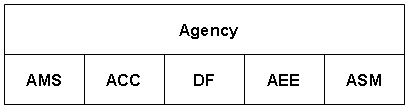
\includegraphics[scale=0.5]{figure/mobilec_lib_arch}
   \caption{Architecture of the Mobile-C library.}
   \label{fig:mobilec_lib_arch}
\end{center}
\end{figure*}
% FIGURE }}} 
%%%%%%%%%%%%%%%%%%%%%%%%%%%%%%%%%%%%%%%%%%%%%%%%%%%%%%%%%%%%%%%%%%%%%%

%%%%%%%%%%%%%%%%%%%%%%%%%%%%%%%%%%%%%%%%%%%%%%%%%%%%%%%%%%%%%%%%%%%%%%
% FIGURE {{{ 
\begin{figure*}[!t]
\begin{center}
   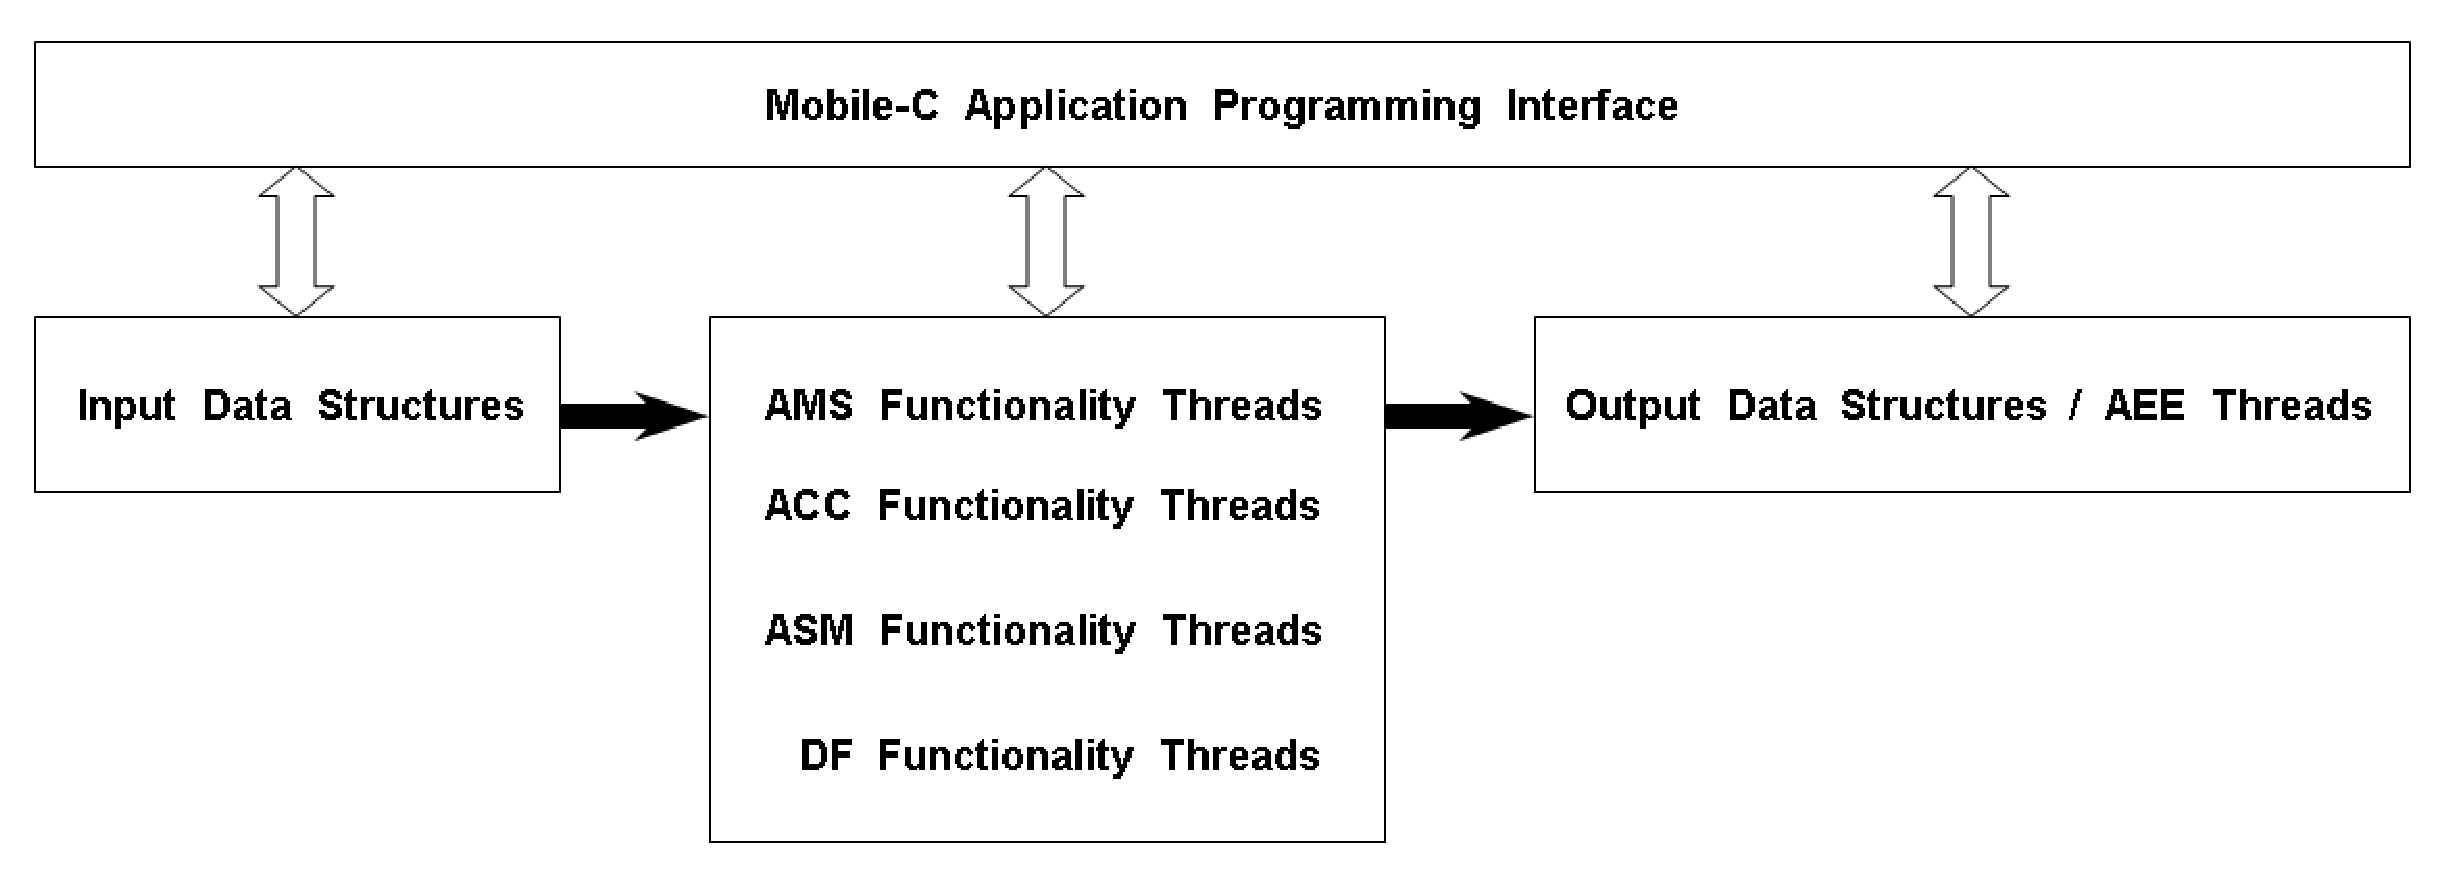
\includegraphics[scale=0.5]{figure/mobilec_lib_imp}
   \caption{Implementation overview of the Mobile-C library.}
   \label{fig:mobilec_lib_imp}
\end{center}
\end{figure*}
% FIGURE }}} 
%%%%%%%%%%%%%%%%%%%%%%%%%%%%%%%%%%%%%%%%%%%%%%%%%%%%%%%%%%%%%%%%%%%%%%

%%%%%%%%%%%%%%%%%%%%%%%%%%%%%%%%%%%%%%%%%%%%%%%%%%%%%%%%%%%%%%%%%%%%%%
% Architecture of the Mobile-C Library {{{
\subsection{Architecture of the Mobile-C Library \label{mobilec_arch}}
Figure \ref{fig:mobilec_lib_arch} illustrates the architecture of the 
Mobile-C library.
The Mobile-C library allows a Mobile-C agency to be embedded in a program to 
support C/C++ mobile agents.
A Mobile-C agency refers to a mobile agent platform within which mobile agents 
exist and operate.
The Mobile-C API gives users a full control over a Mobile-C agency and its 
different modules.
 
As a IEEE FIPA compliant mobile agent platform, a Mobile-C agency 
comprises three FIPA normative modules, Agent Management System (AMS), 
Agent Communication Channel (ACC) and Directory Facilitator (DF). 
Two additional modules, Agent Execution Engine (AEE) and 
Agent Security Manager (ASM), are included in a Mobile-C agency as well.
These modules provide different functionalities summarized as follows.

\textit{Agent Management System (AMS)}

\noindent
An AMS controls the creation, registration, execution, migration, 
persistence, and termination of a mobile agent. 
It maintains a directory of Agent Identifiers (AIDs) for registered mobile 
agents. 
Each mobile agent must register with an AMS in order to have a valid AID.

\textit{Agent Communication Channel (ACC)}

\noindent
An ACC routes messages between local and remote entities. 
It is responsible for the interactions between distributed components, such 
as inter-agent communication and inter-platform agent transport. 
The interactions can be performed through Agent Communication Language (ACL) 
message exchange.

\textit{Directory Facilitator (DF)}

\noindent
A DF serves yellow page services. 
Mobile agents wishing to advertise their services should register with a DF. 
Visiting mobile agents can search a DF for mobile agents providing the 
services they desire.

\textit{Agent Execution Engine (AEE)}

\noindent
An AEE serves as the execution environment for mobile agent code.
An AEE has to be platform independent in order to support the execution of 
mobile agents in a heterogeneous environment. 

Each AEE contains an Embedded Ch interpreter to interpret the agent C code.
By default, the agency will preload four interpreters upon startup for
interpreting agents. If more than four interpreters are required, the agency
will dynamically allocate extra interpreters as needed. See the reference for
\texttt{MC\_Initialize()} on page \pageref{api:MC_Initialize} for more info.

\textit{Agent Security Manager (ASM)}

\noindent
An ASM is responsible for maintaining securita policies for the host system.
Some sample tasks of an ASM include identifying users, protecting host 
resources, authenticating and authorizing mobile agents, and ensuring the 
security and integrity of mobile agents.
% }}} Architecture of the Mobile-C Library
%%%%%%%%%%%%%%%%%%%%%%%%%%%%%%%%%%%%%%%%%%%%%%%%%%%%%%%%%%%%%%%%%%%%%%

%%%%%%%%%%%%%%%%%%%%%%%%%%%%%%%%%%%%%%%%%%%%%%%%%%%%%%%%%%%%%%%%%%%%%%
% SUB: Implementation of the Mobile-C Library {{{
\subsection{Implementation of the Mobile-C Library}
Figure \ref{fig:mobilec_lib_imp} shows the implementation overview of the 
Mobile-C library.
The functionalities of each module of an agency are 
implemented as independent threads classified into five categories, that is, 
the AMS functionality threads, the ACC functionality threads, the DF 
functionality threads, the ASM functionality threads and the AEE threads.
Each AEE thread is launched by one of the AMS functionality threads.

The Mobile-C library provides API functions to specify which thread needs to 
be active or inactive when an agency is initialized.
It also provides API functions to access the input and output data structures 
associated with the functionality threads.
A Mobile-C agency maintains a list of synchronization variables that can be 
used with a group of Mobile-C functions to ensure synchronization among 
mobile agents and threads.
The sizes of the Mobile-C static and shared libraries for Linux are about 
500 KB and 390 KB, respectively.

The header file \textit{libmc.h} contains definitions of all the structures and 
functions of the Mobile-C library. 
Table \vref{mobilec_api_cbinary} lists the currently implemented functions 
for the binary space.

% }}} Implementation of the Mobile-C Library
%%%%%%%%%%%%%%%%%%%%%%%%%%%%%%%%%%%%%%%%%%%%%%%%%%%%%%%%%%%%%%%%%%%%%%

% }}} The Mobile-C Library
%%%%%%%%%%%%%%%%%%%%%%%%%%%%%%%%%%%%%%%%%%%%%%%%%%%%%%%%%%%%%%%%%%%%%%

% }}} Getting Started
%%%%%%%%%%%%%%%%%%%%%%%%%%%%%%%%%%%%%%%%%%%%%%%%%%%%%%%%%%%%%%%%%%%%%%

%%%%%%%%%%%%%%%%%%%%%%%%%%%%%%%%%%%%%%%%%%%%%%%%%%%%%%%%%%%%%%%%%%%%%%
% Composing Agents {{{
\chapter{Composing Agents}
Mobile-C agents are represented internally as XML data structures. However,
dealing with XML code requires background knowledge of XML and may be cumbersome.
To enhance the convenience of creating and deploying Mobile-C agents,
several different methods of creating agents from C source code files have
been implemented.

Agents may be composed from plain C source code. There are two main ways to
compose Mobile-C agents. Agents may be composed by using the
\texttt{compose\_send} commmand in the Mobile-C prompt, or by using the
\texttt{MC\_ComposeAgent*} series of API functions.

\section{Mobile-C Command Prompt \texttt{compose\_send} Command}
The \texttt{compose\_agent} takes a C source code file and creates
a fully functioning agent out of it. The \texttt{compose\_send} command
syntax is
\begin{verbatim}
compose_send <filename> <target host> <target port>
\end{verbatim}
Many details about an agent generated in this method, such as the agent's
name and owner, are dynamically generated when creating an agent using 
this method. 
\subsection{Example Execution Using the \texttt{compose\_send} Command}
The demo \texttt{prompt\_example} has been provided with the Mobile-C
package. Note that the source code for both servers is virtually identical to
that in Program \ref{prog:server.c}, except with added execution
instructions.
The demo program is initiated by starting the first agency, named
\texttt{server1}.
\begin{verbatim}
$ ./server1
Agency 1 started. Please start the second agency by running the command
"server2" on another terminal.

MobileC >
\end{verbatim}
Next, the second agency is started on a seperate terminal.
\begin{verbatim}
$ ./server2
Starting Agency...
You may now try the following commands:

  compose_send helloworld.c localhost 5050

The previous command will compose an agent using the source
code in "helloworld.c" and send it to the other agency at
port 5050. Then try this command:

  compose_send helloworld.c localhost 5051

This will send the "hello_world.c" agent to the local agency.
You may also try these commands at the other agency.

MobileC >
\end{verbatim}
Following the instructions on the second agency, we execute the 
suggested \texttt{compose\_send} command. The first agency terminal
now appears as such:
\begin{verbatim}
$ ./server1
Agency 1 started. Please start the second agency by running the command
  "server2" on another terminal.

MobileC > Hello, world!
\end{verbatim}
Note that the source file \texttt{helloworld.c} has been composed into a 
mobile agent, migrated to the \texttt{server1} agency, and executed.

\section{Mobile-C \texttt{MC\_ComposeAgent*} Functions}
There also exist a set of API functions which compose agents from C source
files. These functions are
\begin{itemize}
\item \texttt{MC\_ComposeAgent()} : Compose an agent from program source code. 
\item \texttt{MC\_ComposeAgentWithWorkgroup()} : Compose an agent from program source code with a workgroup code. 
\item \texttt{MC\_ComposeAgentFromFile()} : Compose an agent from a program source code file. 
\item \texttt{MC\_ComposeAgentFromFileWithWorkgroup()} : Compose an agent from a program source code file with a workgroup code. 
\item \texttt{MC\_AgentAddTask()} : Add an additional task to an already formed agent.
\item \texttt{MC\_AgentAddTaskFromFile()} : Add an additional task to an already formed agent from a C source code file.
\end{itemize}
For an example of the usage of these functions, please refer to program
\ref{prog:compose_multi_task_agent}.

\begin{Program}[p]
\begin{center}
   {\footnotesize \linespread{1.0}
     \verbatiminput{../demos/composing_agents/multi_task_example/client_abridged.c}}
\end{center}
\caption{An agency building an agent with multiple tasks from seperate source code files.}
\label{prog:compose_multi_task_agent}
\end{Program}

\section{Agent Workgroups}
In order to provide an added layer of organization and security, agents
may be created which belong to a workgroup. A workgroup's name may be an
ASCII text string of any length. If an agent belongs in a workgroup,
then certain actions on that agent may only be performed by other agents
in the same workgroup. Thus, if a group of agents keeps their workgroup
name private, no agents outside of that group will be able to terminate,
delete, or otherwise affect the agents within the workgroup. All agents are
still able to interact through FIPA ACL messages.

For an example of agent workgroups in action, please see the demo program
in the\\
 \texttt{demos/agent\_workgroup\_example} directory. 
% }}}
%%%%%%%%%%%%%%%%%%%%%%%%%%%%%%%%%%%%%%%%%%%%%%%%%%%%%%%%%%%%%%%%%%%%%%


%%%%%%%%%%%%%%%%%%%%%%%%%%%%%%%%%%%%%%%%%%%%%%%%%%%%%%%%%%%%%%%%%%%%%%
% Agent Data {{{
\chapter{Agent Data}
Agents have the ability to carry pieces of data with them as they migrate from
host to host. The data carried by an agent can be categorized into two broad
types: ``agent return data'' and ``agent saved variables''. 

\section{Agent Return Data}
  ``Agent return data'' is typically used to store a piece of data being
returned to the agent's home agency. For instance, if an agent is given a task
to obtain a single result from a remote host, the agent might store the result
as its agent return data. An agent may hold a single return value for each one
of its tasks. The return value may be of any standard C type, or an array of 
such a type. For instance, the \texttt{double} type, as well as
\texttt{double[5][3]} are both valid types for a piece of agent return data,
since both are examples of a standard C type or an array of a standard type.
User defined structs and unions may not be returned as a piece of return data.
 
In order to return a variable as agent return data, the name of the return variable
simply needs to be specified when composing the agent. No further API calls need to be
executed from within the agent code. Note that the return variable must be declared as
a global variable in the agent code.
For an example of an agent with multiple tasks returning information to its home agency,
please see Program \ref{prog:compose_multi_task_agent} on page
\pageref{prog:compose_multi_task_agent}.

\section{Agent Saved Variables} 
An ``agent saved variable'' is also carried with an agent as it migrates. However,
this type of variable is typically used for data that the agent itself has access
to as it completes its tasks. Furthermore, an agent may save the value of as many
variables as it desires per task. For instance, during an agent's first task, it
may save various values, like the number of other agents on the agency as an
\texttt{int}, and the name of the agency as a \texttt{char[80]}. After it
migrates to it's second task, it may access the variables it saved previously
on the first host. In this way, an agent could calculate the total number of
active agents in an agency network. In summary,

\begin{tabular}{l|cc}
 & Agent Return Data & Agent Saved Variable \\
\hline
May save multiple variables per task & & X \\
\hline
Data easily retrieved by home agency & X & X \\
\hline
Data saved to agent automatically  & & \\
without agent-space API calls & X & \\
\hline
Agent can access its own saved data & & X
\end{tabular}

\vspace{0.18in}
For example, consider an agent with the following tasks. The agent's first task
appears as such:
\verbatiminput{../demos/agent_migration_message_format/agent_saved_variables_example/task1.c}
Note that the variable to be saved must be a global variable. In the agent code, the agent
performs a call to the function \texttt{mc\_AgentVariableSave(mc\_current\_agent, "savevar");}
The first argument in the function is a handle to an agent. The handle \texttt{mc\_current\_agent} is
a special handle an agent has to itself. The second argument is a character string denoting the
name of the variable to save. In effect, this code saves the value of \texttt{savevar} to
itself. As shown in the preceding code, the \texttt{mc\_AgentVariableSave()} function may
be called multiple times on differing variable types and arrays. Each variable will be
saved to the agent prior to migration.

Here is an example of the agent's second task's code:
\verbatiminput{../demos/agent_migration_message_format/agent_saved_variables_example/task2.c}
Note the call to \texttt{mc\_AgentVariableRetrieve(mc\_current\_agent,
"savevar", 0);} in this code example. This function attempts to retrieve a
pointer to the saved variable. The first argument, as seen before, is a handle
to the agent itself. The second variable is the name of the variable to
retrieve. The third argument is the task from which to retrieve the variable,
with the value \texttt{0} being the first task. If the call succeeds, it will
return a valid pointer to the saved variable. If it fails, the function returns
\texttt{NULL}.



% Chapter: Agent Data }}}
%%%%%%%%%%%%%%%%%%%%%%%%%%%%%%%%%%%%%%%%%%%%%%%%%%%%%%%%%%%%%%%%%%%%%%


%%%%%%%%%%%%%%%%%%%%%%%%%%%%%%%%%%%%%%%%%%%%%%%%%%%%%%%%%%%%%%%%%%%%%%
% Mobile-C Agent Migration Message Format {{{
\chapter{Mobile-C Agent Migration Message Format}
\section{General Message Format \label{sec:gen_message_format}}
\begin{Program}
\begin{center}
   {\scriptsize \linespread{1.0} \verbatiminput{../demos/getting_started/hello_world/test1.xml}}
\end{center}
\caption{A rudimentary agent. (demos/getting\_started/hello\_world/test1.xml)}
\label{prog:hello_agent}
\end{Program}
The message format for an agent migration message is designed such that
multiple tasks and multiple code blocks can be migrated from agency to
agency. The message is an XML message with encapsulated C code. An example
of a rudimentary agent can be seen in Program \ref{prog:hello_agent} on 
page \pageref{prog:hello_agent}. 
Following is a brief description of each XML tag.
\begin{itemize}
\item \texttt{MESSAGE}: This tag indicates to Mobile-C that the following data
  is a Mobile-C message. The message type is included in the attribute
  ``message''.
\item \texttt{MOBILE\_AGENT}: This tag indicates that the contained data is a 
  Mobile-C agent.
\item \texttt{AGENT\_DATA}: This tag indicates that the contained data is data pertaining
  to this particular agent.
\item \texttt{NAME}: The name of the agent.
\item \texttt{OWNER}: The owner of the agent. 
\item \texttt{HOME}: The home of the agent. Any agent that has data to ``return'' will
	return it to this address by default.
\item \texttt{WG\_CODE}: The workgroup code of the agent. Workgroup codes are
kept secret by the agent. Only agents with matching workgroup codes are allowed
to perform certain operations on each other, such as agent deletion.
\item \texttt{TASKS}: This indicates that the following information pertains to the
  task or tasks the agent is intended to perform. Attributes found under the
  \texttt{TASKS} tag include:
  \begin{itemize}
    \item \texttt{task} : The total number of tasks the agent has.
    \item \texttt{num} : The task that the agent is currently on.
  \end{itemize}
\item \texttt{TASK}: Each seperate \texttt{TASK} tag indicates a seperate task for the agent
  to perform. The tasks may be seperate hosts and/or code blocks. In the
  rudimentary example, there is only one task. Listed below are the attributes of 
  \texttt{TASK} tags.
  \begin{itemize}
  \item \texttt{num}:           The number of the task. The first task is task number zero.
  \item \texttt{complete}:      Completeness of the task
  \item \texttt{server}:        The host to perform the task
  \item \texttt{return}:        Name of the return variable
  \item \texttt{persistent}:    Persistence of the agent
  \item \texttt{return\_value}: Return value, if not an array
  \item \texttt{code\_id}:      ID of the code block to execute
  \end{itemize}
\textit{complete} and \textit{server} are mandatory attributes, and others are 
optional attributes.  
\item AGENT\_CODE: Each AGENT\_CODE block represents a block of code that 
  the agent may execute. Agents with multiple code blocks may decide at run-time
  which block to execute. Valid attributes under the \texttt{AGENT\_CODE} tag
  include
  \begin{itemize}
    \item \texttt{id}: The id of the code segment, as referenced by the \texttt{TASK} 
      attribute, \texttt{code\_id}.
  \end{itemize}
\end{itemize}

\section{Multiple Tasks with a Single Code Block}
An agent may have an indefinite number of tasks. The agent will perform the tasks
in ther order that they are stated in the XML file, completing each one before
continuing to the next host. Following is an example of an agent which has
multiple tasks to perform, executing the same code block at each new host.
See Program \ref{prog:single_code_block} on page \pageref{prog:single_code_block} 
for an example.
\begin{Program}[p]
\begin{center}
   {\footnotesize \linespread{1.0} 
     \verbatiminput{../demos/composing_agents/multi_task_example/test_single_code_block1.xml}}
\end{center}
\caption{An example agent containing two tasks and a single code block.
  Note that variables ``mc\_host\_name'' and ``mc\_task\_progress'' are special built-in variables described in Table \vref{tab:agent_space_variables}.
  \index{mc\_host\_name}
  \index{mc\_task\_progress}
  \texttt{(<MCPACKAGE>/demos/composing\_agents/multi\_task\_example/test\_single\_code\_block.xml)} }
\label{prog:single_code_block}
\end{Program}
\addtocounter{Program}{-1}
\begin{Program}[p]
\begin{center}
   {\footnotesize \linespread{1.0} 
     \verbatiminput{../demos/composing_agents/multi_task_example/test_single_code_block2.xml}}
\end{center}
\caption{(Continued)}
\end{Program}

\section{Multiple Tasks with Multiple Code Blocks}
See Program \ref{prog:multi_code_block} on page \pageref{prog:multi_code_block}
for a more complicated example of agent code including multiple tasks and
  multiple code blocks. Note that each code block has an associated ID which is 
  refered to in the respective ``DATA'' tags. Also note that more than one ``DATA'' tag
  may refer to the same code block. Thus, an agent may have more ``DATA'' tags than
  code blocks.

\begin{Program}[p]
\begin{center}
   {\footnotesize \linespread{1.0} 
     \verbatiminput{../demos/composing_agents/multi_task_example/test_multi_code_block1.xml}}
\end{center}
\caption{An example agent containing two tasks and two code blocks. 
  \texttt{(<MCPACKAGE>/demos/composing\_agents/multi\_task\_example/test\_multi\_code\_block.xml)}} 
\label{prog:multi_code_block}
\end{Program}
\addtocounter{Program}{-1}
\begin{Program}[p]
\begin{center}
   {\footnotesize \linespread{1.0} 
     \verbatiminput{../demos/composing_agents/multi_task_example/test_multi_code_block2.xml}}
\end{center}
\caption{ (Continued) }
\end{Program}

\section {Multiple Mobile Agent performs Task on Multiple Hosts}
Program \ref{prog:multi_mobile_agent_client} on page \pageref{prog:multi_mobile_agent_client} is a client that sends two different mobile agents to two different hosts. In for loop, it waits for the arrival signal of mobile agent. When an agent arrives it prints the result and delete that agent. For loop is iterated same as total number of mobile agents send by client. The two mobile agents having different name are shown in Program \ref{prog:mobile_agent_1} and Program \ref{prog:mobile_agent_2}:  

\begin{Program}[p]
\begin{center}
   {\footnotesize \linespread{1.0}
     \verbatiminput{../demos/agent_migration_message_format/multi_data_retrieval/client.c}}
\end{center}
\caption{A client program that sends two mobile agents to two different hosts
  \texttt{(<MCPACKAGE>/demos/agent\_migration\_message\_format/multi\_data\_retrieval/client.c)}}
\label{prog:multi_mobile_agent_client}
\end{Program}

\begin{Program}[p]
\begin{center}
   {\footnotesize \linespread{1.0}
     \verbatiminput{../demos/agent_migration_message_format/multi_data_retrieval/test1.xml}}
\end{center}\caption{First mobile agent name "mobagent1" send by client (Program 6) to server 1   
  \texttt{(<MCPACKAGE>/demos/agent\_migration\_message\_format/multi\_data\_retrieval/test1.xml)}}
\label{prog:mobile_agent_1}
\end{Program}

\begin{Program}[p]
\begin{center}
   {\footnotesize \linespread{1.0}
     \verbatiminput{../demos/agent_migration_message_format/multi_data_retrieval/test2.xml}}
\end{center}\caption{Second mobile agent name "mobagent1" send by client (Program 6) to server 2
  \texttt{(<MCPACKAGE>/demos/agent\_migration\_message\_format/multi\_data\_retrieval/test2.xml)}}
\label{prog:mobile_agent_2}
\end{Program}

\section{Agent Return Messages}
If the ``\texttt{name}'' attribute in an agent's ``\texttt{DATA}'' tag
is not set to ``\texttt{no-return}'', the agent will generate an
agent-return message upon completion of all of its tasks. The agent will
generate a return message containing the contents of the variable name
specified in the ``\texttt{name}'' attribute. For instance, Program
\vref{prog:agent_with_return_data} shows a simple agent which 
will migrate to another agency, generate a three-dimensional array called
``\texttt{a}'', and return the contents of the array to the ``\texttt{HOME}''
host upon completion. Note that the return variable must be global
so that the contents are not destroyed upon completion of the \texttt{main}
function. 
  
  An example of the return message that is generated by
this agent can be seen in Program \vref{prog:return_agent}. Notice also in
the return message that the variable type has been changed from ``int'' as it
was in the original program to ``short'' and that the ``\texttt{dim}'' attribute
has been changed to $3$. This is because Mobile-C automatically
checks the type and dimension of the variable it is returning and assign
those attributes automatically.

\begin{Program}[p]
\begin{center}
   {\footnotesize \linespread{1.0} 
     \verbatiminput{../demos/agent_migration_message_format/mc_array_return_example/agent.xml}}
\end{center}
\caption{An agent which returns data upon completion of it's tasks.}
\label{prog:agent_with_return_data}
\end{Program}

\begin{Program}[p]
\begin{center}
   {\footnotesize \linespread{1.0} 
     \verbatiminput{../demos/agent_migration_message_format/mc_array_return_example/return_agent.xml}}
\end{center}
\caption{Agent return data xml format. Note: This XML code has been reformatted
  to a more human-readable format. The actual format generated may differ.}
\label{prog:return_agent}
\end{Program}

\section{Agent Saved Variables}
As of Mobile-C version 1.10.0, Mobile-C agents have the ability to save an 
arbitrary number of variables while migrating from task to task. Agents may
use the agent-space api functions \texttt{mc\_AgentVariableSave()} and
\texttt{mc\_AgentVariableRetrieve} to save and later retrieve variables.
An example agent which does this may be viewed at the documentation for
the \texttt{mc\_AgentVariableSave()} and \linebreak \texttt{mc\_AgentVariableRetrieve()}
functions on pages \pageref{apidoc:mc_AgentVariableSave} and 
\pageref{apidoc:mc_AgentVariableRetrieve}, respectively.

As the agent is migrating from host to host with saved data, the data is 
encapsulated in the agent's XML code. \texttt{<DATA>} tags are created as
children of each \texttt{<TASK>} tag to store data. See Program 
\ref{prog:migrating_agent} for an example of an agent that is migrating
with saved data. The valid attributes within a \texttt{<DATA>} tag are
\begin{itemize}
\item \texttt{name}: The name of the saved variable.
\item \texttt{dim}: The array dimension of the saved variable. 
\item \texttt{type}: The type of the variable.
\item \texttt{value}: (optional) If the variable has zero dimensions, the
  value is stored in this attribute. Otherwise, children \texttt{<ROW>} 
  tags must be created to store the array.
\end{itemize}

Each \texttt{<DATA>} tag may also have children \texttt{<ROW>} tags, if
the data is an array. The valid attributes of the \texttt{<ROW>} tags are
\begin{itemize}
\item \texttt{index}: The index of the row.
\end{itemize}
Note also that each \texttt{<ROW>} tag may contain additional \texttt{<ROW>}
children depending on the dimension of the array being stored.

The Mobile-C XML Data Type Definition (DTD), which defines the format of a
well-formed Mobile-C agent migration message, may be seen in Section
\ref{sec:xml_dtd} on page \pageref{sec:xml_dtd}.

\section{Stationary/Persistent Mobile Agents}
A Stationary agent may be achieved in Mobile-C simply by creating an agent which
never migrates. This is commonly achieved using a couple of different
techniques.
\subsection{An Agent with an Infinite Task}
An agent may be considered stationary if it's task never ends. For instance, if
the task of an agent is of the form:
\begin{verbatim}
while(1)
{
    cmd = wait_for_command();
    execute_command(cmd);
}
\end{verbatim}
Since the previous task never ends, the agent will never terminate and the agent
will remain stationary in it's agency. 

\subsection{The ``\texttt{persistent}'' Agent Flag}
The ``\texttt{persistent}'' flag as mentioned in Section
\ref{sec:gen_message_format} may be used to create a persistent agent. The
example described in Chapter \ref{chap:interface_binary_to_agent} uses such a
technique. This technique creates an agent which is not automatically flushed by the agency
after it completes it's task. Thus, the agent remains dormant and stationary in
the agency without external stimulus.

\subsubsection{Terminating Persistent Agents}
Persistent agents should be terminated when they are no longer needed to free
up resources. They may be terminated by using the API functions 
\texttt{MC\_DeleteAgent()} or \texttt{MC\_TerminateAgent()} functions from C-space,
or the functions \texttt{mc\_DeleteAgent()} or \texttt{MC\_TerminateAgent()} functions 
from agent-space. Since a persistent agent cannot terminate itself, it is up to either
the host agency or another agent to terminate the persistent agent.

\begin{Program}[ph]
\begin{center}
{\footnotesize \linespread{1.0}
\verbatiminput{../demos/agent_migration_message_format/agent_saved_variables_example/migrating_agent.xml.part1}}
\end{center}
\caption{\label{prog:migrating_agent} This XML format illustrates an agent which is currently
in the process of migrating with saved data. Note that the agent contains two tasks, and the
first task has been completed. This file is a snapshot of the agent as it is in transit from
task '0' to task '1'. Note the \texttt{<DATA>} tags which store the three variables
referenced by the \texttt{mc\_AgentSaveVariable()} function from within the code, storing
two integers and an integer array. Note that in general, any data type may be stored, including
multi-dimensional arrays.}
\end{Program}
\addtocounter{Program}{-1}
\begin{Program}[ph]
\begin{center}
{\footnotesize \linespread{1.0}
\verbatiminput{../demos/agent_migration_message_format/agent_saved_variables_example/migrating_agent.xml.part2}}
\end{center}
\caption{(Continued)}
\end{Program}


% }}} Mobile-C Agent Migration Message Format
%%%%%%%%%%%%%%%%%%%%%%%%%%%%%%%%%%%%%%%%%%%%%%%%%%%%%%%%%%%%%%%%%%%%%%

%%%%%%%%%%%%%%%%%%%%%%%%%%%%%%%%%%%%%%%%%%%%%%%%%%%%%%%%%%%%%%%%%%%%%%
% {{{ Mobile-C FIPA Compliant ACL Messages
\chapter{Mobile-C FIPA Compliant ACL Messages \label{chap:fipa}}
Mobile-C has the ability to send and receive FIPA compliant
agent communication language (ACL) messages. More information
about FIPA, the Foundation for Intellegent Physical Agents, may be
found at \texttt{http://www.fipa.org}. This functionality allows
Mobile-C agent to communicate with each other, as well as with 
agents from other agencies that are also FIPA compliant. Demos
of communication with JADE agents may be found in the directories
\texttt{<MCPACKAGE>/demos/jade\_to\_mc\_example} and \\
\texttt{<MCPACKAGE>/demos/mc\_to\_jade\_example}.

%{{{ Constructing and Sending an ACL Message
\section{Constructing and Sending an ACL Message}
The general process for constructing an ACL message involves
filling out required portions of an ACL message structure of type
\texttt{struct fipa\_acl\_message\_s} and passing the message to the
\texttt{MC\_AclSend()} function. A number of helper functions 
exist in order to simplify the process of allocating memory and setting
certain fields of the acl message. 
Some typical functions used to compose a new ACL message are the following:
\begin{itemize}
\item \texttt{MC\_AclSetPerformative}: Set the FIPA performative of the message. See Program
  \ref{prog:fipa_enum} for a complete listing of valid FIPA performative enumerations.
\item \texttt{MC\_AclSetSender}: Sets the 'sender' field of the message.
\item \texttt{MC\_AclAddReceiver}: Adds addresses to the 'receiver' field of the message.
\item \texttt{MC\_AclSetContent}: Sets the 'content' field of an ACL message.
\end{itemize}
A detailed example of sending and receiving messages will be presented in
Chapter \ref{chap:stationary_agent}.
%}}}

%{{{Receiving an ACL Message 
\section{Receiving an ACL Message}
Every agent residing on a Mobile-C agency has a mailbox allocated to it.
At any time, the agent may check the mailbox for new ACL messages, or an
agent may choose to wait on an empty mailbox until a new message arrives.
These two tasks are done by the functions \texttt{MC\_AclRetreive()} and
\texttt{MC\_AclWaitRetrieve()}, respectively. 
Another useful function which may be used with a received ACL message is the
\texttt{MC\_AclReply()} function. This function takes an ACL message as an
input argument and automatically forms an ACL reply message addressed to the
original sender. Note that the performative and new sender fields in the reply
message are not automatically initialized and will still need to be set by
the agent. A detailed example of an agent receiving and replying to a message
may be found in Chapter \ref{chap:stationary_agent}.

\begin{Program}[!t]
\begin{center}
   {\footnotesize \linespread{1.0} 
\begin{verbatim}
enum fipa_performative_e
{
  FIPA_ERROR=-1,
  FIPA_ZERO,
  FIPA_ACCEPT_PROPOSAL,
  FIPA_AGREE,
  FIPA_CANCEL,
  FIPA_CALL_FOR_PROPOSAL,
  FIPA_CONFIRM,
  FIPA_DISCONFIRM,
  FIPA_FAILURE,
  FIPA_INFORM,
  FIPA_INFORM_IF,
  FIPA_INFORM_REF,
  FIPA_NOT_UNDERSTOOD,
  FIPA_PROPOGATE,
  FIPA_PROPOSE,
  FIPA_PROXY,
  FIPA_QUERY_IF,
  FIPA_QUERY_REF,
  FIPA_REFUSE,
  FIPA_REJECT_PROPOSAL,
  FIPA_REQUEST,
  FIPA_REQUEST_WHEN,
  FIPA_REQUEST_WHENEVER,
  FIPA_SUBSCRIBE
};
\end{verbatim}
   }
\end{center}
\caption{Fipa Performative Enumerations.}
\label{prog:fipa_enum}
\end{Program}

\pagebreak
\clearpage
\pagebreak
%}}} Section: Receiving an ACL Message

%}}} Chapter: Mobile-C FIPA Compliant ACL Messages
%%%%%%%%%%%%%%%%%%%%%%%%%%%%%%%%%%%%%%%%%%%%%%%%%%%%%%%%%%%%%%%%%%%%%%

%%%%%%%%%%%%%%%%%%%%%%%%%%%%%%%%%%%%%%%%%%%%%%%%%%%%%%%%%%%%%%%%%%%%%%
% Mobile-C Binary Stationary Agents {{{
\chapter{Mobile-C Binary Stationary Agents \label{chap:stationary_agent}}
Mobilec has support for hosting binary-space stationary agents. The
agents are implemented as system threads. As such, the only limit 
to the number of stationary agents residing on an agency are the
system resources of the host agency. 

The binary agents are able to call any of the C-space API functions, such as
\texttt{MC\_AclWaitRetrieve()}. This allows stationary agents to communicate
and interact with other mobile and stationary agents using FIPA ACL messages,
as introduced in Chapter \ref{chap:fipa}.

Stationary agents may be used in any application in which agent mobility is
unnecessary. Stationary agents can typically perform any task a mobile agent
can perform, except migration. Furthermore, stationary agents tend to execute
faster and consume less system resources.

Mobile-C stationary agent threads are added using the
\texttt{MC\_AddStationaryAgent()} API function. See Program 
\ref{prog:stationary_agent_server} for an example of a stationary agent. 

\begin{Program}[!t]
\begin{center}
   {\footnotesize \linespread{1.0} \verbatiminput{../demos/binary_stationary_agents/stationary_agent_communication/server.c}}
\end{center}
\caption{A sample program which starts a single stationary agent that responds to FIPA ACL messages.}
\label{prog:stationary_agent_server}
\end{Program}

The \texttt{MC\_AddStationaryAgent()} function takes three arguments:
\begin{enumerate}
\item A handle to the home agency. This is the agency the new agent will reside under.
\item The agent thread. This is a pointer to a function which will execute and act as
the stationary agent. If the function returns, the stationary agent is terminated.
\item An optional argument to pass to the agent. If additional information or data needs
to be passed to the stationary agent thread, a pointer of any type may be supplied as the
third argument to \\
\texttt{MC\_AddStationaryAgent()}. This pointer may later be retrieved
with the \\
\texttt{MC\_AgentInfo\_GetAgentArgs()} function from within the agent.
\end{enumerate}

The stationary agent thread must have a prototype of the form
\begin{verbatim}
void* agent_func_name(stationary_agent_info_t* agent_info);
\end{verbatim}
As seen in the prototype, the agent thread receives an argument of type
\texttt{stationary\_agent\_info\_t}. This special type is a structure 
which contains information about the the agent, such as its name, and the
location of its mailbox. Certain information may be retrieved from the 
function parameter by using the \texttt{MC\_AgentInfo\_*} series of API
functions, which include:
\begin{itemize}
\item \texttt{MC\_AgentInfo\_GetAgency()} : Retrieves a handle to the host agency.
\item \texttt{MC\_AgentInfo\_GetAgent()} : Retrieves a handle to the agent
information structure.
\item \texttt{MC\_AgentInfo\_GetAgentArgs()} : Retrieves the pointer that was
given as an agent argument during the call to \texttt{MC\_AddStationaryAgent}.
\end{itemize}

Example usage of these functions may be seen in Program \ref{prog:stationary_agent_server}.
%}}}
%%%%%%%%%%%%%%%%%%%%%%%%%%%%%%%%%%%%%%%%%%%%%%%%%%%%%%%%%%%%%%%%%%%%%%

%%%%%%%%%%%%%%%%%%%%%%%%%%%%%%%%%%%%%%%%%%%%%%%%%%%%%%%%%%%%%%%%%%%%%%
% Interface between Binary and Mobile Agent Spaces {{{
\chapter{Interface between Binary and Mobile Agent Spaces
\label{chap:interface_binary_to_agent}}
An embeddable C/C++ interpreter Ch was chosen to be the AEE in the Mobile-C 
library to support C/C++ mobile agents. 
Therefore, in order to access the variables, functions, and data sets in 
the mobile agent space from the binary space, Ch must be first embedded in the 
binary space.
The function \textit{MC\_GetAgentExecEngine()} \index{MC\_GetAgentExecEngine()} in 
Table \ref{mobilec_api_cbinary} returns the AEE associated with a mobile agent 
to the binary space.
Using the AEE returned by \textit{MC\_GetAgentExecEngine()}, all of the 
Embedded Ch functions~\cite{EmbeddedCh} can be called in a binary C/C++ 
program to access the variables, functions, and data sets defined in the 
mobile agent space.
The Embedded Ch toolkit also allows mobile agent code to invoke C/C++ 
functions defined in a binary C/C++ program.

The Embedded Ch toolkit reduces the complexity of heterogeneous development 
environment for both embedded scripting and applications. 
With the consistent C/C++ code base, it can significantly reduce the effort 
in the software development and maintenance. 
Moreover, with the Embedded Ch toolkit, C/C++ applications can be extended 
with all the features of Ch including built-in string type for scripting. 
The Embedded Ch toolkit has a small footprint. 
The pointer and time deterministic nature of the C language provide a 
perfect interface with hardware in real-time systems.

\section{Using an Agent Initialization Callback Function to Intergrate Binary
and Script Space Code}
The user may register a callback function to be called during the initialization
of mobile agents inside of an agency. This allows the user to fine-tune 
an agent and the Ch interpreter before an agent is executed. The callback
function is added using the \texttt{MC\_AddAgentInitCallback()} function,
and the callback function is of the form
\begin{verbatim}
int callback(ChInterp_t interp, MCAgent_t agent, void* user_data);
\end{verbatim}
The user may call any applicable Ch API function on the interpreter,
as well as any applicable Mobile-C API function on the supplied agent.
For instance, the user may use the \texttt{Ch\_DeclareVar()} function
to declare extra variables inside of the interpereter which the agent
will be able to access during its execution. 

The demo located at \texttt{demos/cspace-agentspace\_interface/agent\_init\_callback/} 
provides a demonstration of the callback function. This demo uses the callback
function to declare a new function in each of the incoming agent interpreters
called \texttt{mult()}, which simply multiplies two numbers together. This
means that any incoming agent will be able to call the \texttt{mult()} function,
which resides in C-space, from the agent script-space. This demo may also be seen with
the documentation for \texttt{MC\_AddAgentInitCallback()} on page \pageref{api:MC_AddAgentInitCallback()}.

%%%%%%%%%%%%%%%%%%%%%%%%%%%%%%%%%%%%%%%%%%%%%%%%%%%%%%%%%%%%%%%%%%%%%%
% Invoke a Mobile Agent Space Function from Binary Space {{{
\noindent
\section{Invoke a Mobile Agent Space Function from Binary Space}
%%%%%%%%%%%%%%%%%%%%%%%%%%%%%%%%%%%%%%%%%%%%%%%%%%%%%%%%%%%%%%%%%%%%%%
% client.c {{{
\begin{Program}[!t]
\begin{center}
   {\footnotesize \linespread{1.0} 
     \verbatiminput{../demos/cspace-agentspace_interface/persistent_example/client.c}}
\end{center}
\caption{ A program which sends a persistent mobile agent.
  \texttt{(<MCPACKAGE>/demos/cspace-agentspace\_interface/persistent\_example/client.c)}}
\label{prog:client_ex2.c}
\end{Program}
% }}} client.c
%%%%%%%%%%%%%%%%%%%%%%%%%%%%%%%%%%%%%%%%%%%%%%%%%%%%%%%%%%%%%%%%%%%%%%
%%%%%%%%%%%%%%%%%%%%%%%%%%%%%%%%%%%%%%%%%%%%%%%%%%%%%%%%%%%%%%%%%%%%%%
% test1.xml {{{
\begin{Program}[!t]
\begin{center}
   {\footnotesize \linespread{1.0} 
     \verbatiminput{../demos/cspace-agentspace_interface/persistent_example/test1.xml}}
\end{center}
\caption{A persistent mobile agent. Agents marked ``persistent'' are
  not flushed from the agency after they terminate.
    \texttt{(<MCPACKAGE>/demos/cspace-agentspace\_interface/persistent\_example/test1.xml)}}
\label{prog:mobileagent_ex2.xml}
\end{Program}
% }}} test2.xml
%%%%%%%%%%%%%%%%%%%%%%%%%%%%%%%%%%%%%%%%%%%%%%%%%%%%%%%%%%%%%%%%%%%%%%
%%%%%%%%%%%%%%%%%%%%%%%%%%%%%%%%%%%%%%%%%%%%%%%%%%%%%%%%%%%%%%%%%%%%%%
% host.c {{{
\begin{Program}[!t]
\begin{center}
   {\footnotesize \linespread{1.0} 
     \verbatiminput{../demos/cspace-agentspace_interface/persistent_example/server.c}}
\end{center}
\caption{A Mobile-C agency.
 \texttt{(<MCPACKAGE>/demos/cspace-agentspace\_interface/ persistent\_example/server.c)}}
\label{prog:server_ex2.c}
\end{Program}
% }}} host.c
%%%%%%%%%%%%%%%%%%%%%%%%%%%%%%%%%%%%%%%%%%%%%%%%%%%%%%%%%%%%%%%%%%%%%%
%%%%%%%%%%%%%%%%%%%%%%%%%%%%%%%%%%%%%%%%%%%%%%%%%%%%%%%%%%%%%%%%%%%%%%
% FIGURE {{{
\begin{figure*}[!t]
\begin{center}
   {\footnotesize \linespread{1.0} \verbatiminput{../demos/cspace-agentspace_interface/persistent_example/server_output.txt}}
   \caption{Output from the binary server program.}
   \label{fig:example2_output}
\end{center}
\end{figure*}
% FIGURE }}}
%%%%%%%%%%%%%%%%%%%%%%%%%%%%%%%%%%%%%%%%%%%%%%%%%%%%%%%%%%%%%%%%%%%%%%

This example illustrates how to call a function defined in mobile agent 
code by using the Mobile-C library and Embedded Ch toolkit. 
The mobile agent in this example is a persistent agent, which is not removed 
upon termination of its execution.

The client program shown in Program \vref{prog:client_ex2.c} starts a Mobile-C 
agency listening on port \textit{5050} by the function 
\textit{MC\_Initialize()}, and sends a mobile agent to the remote agency 
running on host \textit{localhost} at port \textit{5051} through 
the function \textit{MC\_SendAgentMigrationMessageFile()}. 
The filename including the full path of the mobile agent is specified from the 
standard input.

The mobile agent sent to the remote agency is 
shown in Program \vref{prog:mobileagent_ex2.xml}. 
The name, owner, source machine of the mobile agent are 
\textit{mobagent1}, \textit{IEL}, and 
\textit{localhost:5050}, respectively. 
The mobile agent is persistent since the flag \textit{persistent}\index{persistent} 
is set to 1 
in Program \ref{prog:mobileagent_ex2.xml}.
This flag can be set to 0 or removed by a user for a non-persistent mobile 
agent.
The embedded mobile agent code is a simple but complete C program which 
defines the function \textit{hello()} to be called in the server program. 

As shown in Program \vref{prog:server_ex2.c}, the server program starts a 
Mobile-C agency listening on port \textit{5051} by the 
function \textit{MC\_Initialize()}, and waits for a mobile agent.  
The mobile agent named \textit{mobagentl} is found by the function 
\textit{MC\_FindAgentByName()} \index{MC\_FindAgentByName()}, and the AEE 
associated with the mobile 
agent is obtained by the function \textit{MC\_AgentExecEngine()} 
\index{MC\_AgentExecEngine()}.
The variable returned by \textit{MC\_AgentExecEngine()} is a Ch interpreter of 
data type \textit{ChInterp\_t}. 
This variable is the first parameter for all of the Embedded Ch functions. 
The function \textit{hello()} defined in the mobile agent code is invoked 
by the Embedded Ch function \textit{Ch\_CallFuncByName()}. 

There are several different methods to call functions in mobile agent 
space from the binary space using the Embedded Ch API. 
Here we describe the function \textit{Ch\_CallFuncByName()}
\index{Ch\_CallFuncByName()} used in Program 
\ref{prog:server_ex2.c}.
With \textit{Ch\_CallFuncByName()}, a function defined in the mobile 
agent space can be called by its name. 
The prototype of \textit{Ch\_CallFuncByName()} is shown as follows.

int Ch\_CallFuncByName(ChInterp\_t interp, char *name, void *retval, ...);

The first argument is an instance of the Ch interpreter. 
The second argument is a string containing the name of the function to be 
called. 
The function name is associated with a function defined in mobile agent code. 
The third argument is a pointer containing the address of the return value of 
the called function. 
If the called function takes any arguments, the arguments should be listed 
after the third argument, \textit{retval}. 
\textit{Ch\_CallFuncByName()} returns zero on successful execution or 
non-zero on failure.

The other method of executing the function is through the Mobile-C
api function {\bf MC\_CallAgentFunc()} \index{MC\_CallAgentFunc()}. 
This method is seen in the example program, Program \ref{prog:server_ex2.c}.

Figure \vref{fig:example2_output} shows the output when the binary file 
\textit{server} compiled from Program \ref{prog:server_ex2.c} was executed. 
The string generated and the value returned from the function \textit{hello()} 
were printed to the screen after the Enter key was pressed once the mobile 
agent had arrived. 

% }}} Invoke a Mobile Agent Space Function from Binary Space 
%%%%%%%%%%%%%%%%%%%%%%%%%%%%%%%%%%%%%%%%%%%%%%%%%%%%%%%%%%%%%%%%%%%%%%

% }}} Interface between Binary and Mobile Agent Spaces
%%%%%%%%%%%%%%%%%%%%%%%%%%%%%%%%%%%%%%%%%%%%%%%%%%%%%%%%%%%%%%%%%%%%%%

%%%%%%%%%%%%%%%%%%%%%%%%%%%%%%%%%%%%%%%%%%%%%%%%%%%%%%%%%%%%%%%%%%%%%%
% Extend Mobile-C Functionality to Mobile Agent Space {{{
\chapter{Extend Mobile-C Functionality to Mobile Agent Space}
%%%%%%%%%%%%%%%%%%%%%%%%%%%%%%%%%%%%%%%%%%%%%%%%%%%%%%%%%%%%%%%%%%%%%%
% FIGURE {{{
\begin{figure*}[b]
\begin{center}
   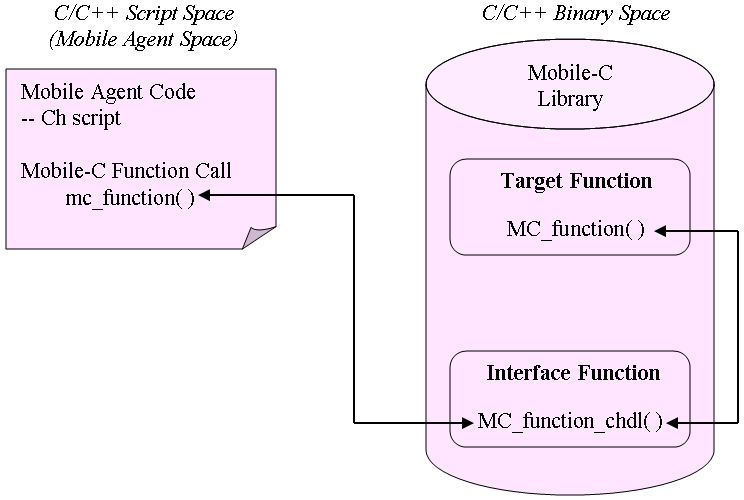
\includegraphics[scale=0.5]{figure/chmobilec_package}
   \caption{Interface of mobile agent code with the Mobile-C library.}
   \label{fig:chmobilec_package}
\end{center}
\end{figure*}
% FIGURE }}}
%%%%%%%%%%%%%%%%%%%%%%%%%%%%%%%%%%%%%%%%%%%%%%%%%%%%%%%%%%%%%%%%%%%%%%
In order to allow mobile agent code to call user defined routines and 
access data sets defined in the binary space, as well as control 
other mobile agents defined in the mobile agent space through the 
Mobile-C API functions, the Mobile-C functionality has to be extended into 
the mobile agent space.
We integrated Ch with the Mobile-C library to provide access to some 
Mobile-C functionalities. 

Figure \vref{fig:chmobilec_package} shows how mobile agent code interfaces 
with the Mobile-C library.
When the function \textit{mc\_function()} is called in mobile agent code,
Ch searches the corresponding interface function \textit{MC\_function\_chdl()} 
in the Mobile-C library, and passes arguments to it by calling the function.
Subsequently, the interface function \textit{MC\_function\_chdl()} invokes the 
target function \textit{MC\_function()}, and passes the return value back to 
the mobile agent space~\cite{EmbeddedCh}.

The prototypes of Mobile-C functions used in the mobile agent space are
declared in \textit{agent.c} through an Embedded Ch function,
\textit{Ch\_DeclareFunc()}.
The data type, \textit{MCAgent\_t}, used as a parameter or return value by 
certain Mobile-C functions for the mobile agent space is also defined in 
\textit{agent.c} by two Embedded Ch functions, 
\textit{Ch\_DeclareVar()} and \textit{Ch\_DeclareTypedef()}~\cite{EmbeddedCh}.
Table \vref{chmobilec_api_cscript} lists the currently implemented functions 
for the mobile agent space.
Two examples are used to demonstrate the applications and features of the 
Mobile-C functionality in the mobile agent space. 

%%%%%%%%%%%%%%%%%%%%%%%%%%%%%%%%%%%%%%%%%%%%%%%%%%%%%%%%%%%%%%%%%%%%%
% Terminate Mobile Agent Execution from Mobile Agent Space {{{
\noindent
\section{Terminate Mobile Agent Execution from Mobile Agent Space}
%%%%%%%%%%%%%%%%%%%%%%%%%%%%%%%%%%%%%%%%%%%%%%%%%%%%%%%%%%%%%%%%%%%%%%
% test2.xml {{{
\begin{Program}[!t]
\begin{center}
   {\footnotesize \linespread{1.0} 
     \verbatiminput{../demos/cspace-agentspace_interface/persistent_example/test2.xml}}
\end{center}
\caption{A mobile agent which enters an infinite loop and does 
  not terminate. \texttt{(<MCPACKAGE>/demos/cspace-agentspace\_interface/persistent\_example/test2.xml)}}
\label{prog:mobileagent1_ex3.xml}
\end{Program}
% }}} test2.xml
%%%%%%%%%%%%%%%%%%%%%%%%%%%%%%%%%%%%%%%%%%%%%%%%%%%%%%%%%%%%%%%%%%%%%%
%%%%%%%%%%%%%%%%%%%%%%%%%%%%%%%%%%%%%%%%%%%%%%%%%%%%%%%%%%%%%%%%%%%%%%
% test3.xml {{{
\begin{Program}[!t]
\begin{center}
   {\footnotesize \linespread{1.0} 
     \verbatiminput{../demos/cspace-agentspace_interface/persistent_example/test3.xml}}
\end{center}
\caption{ This agent terminates the execution
of the agent in Program \ref{prog:mobileagent1_ex3.xml}. 
  \texttt{(<MCPACKAGE>/demos/cspace-agentspace\_interface/persistent\_example/test3.xml)}}
\label{prog:mobileagent2_ex3.xml}
\end{Program}
% }}} test3.xml
%%%%%%%%%%%%%%%%%%%%%%%%%%%%%%%%%%%%%%%%%%%%%%%%%%%%%%%%%%%%%%%%%%%%%%

This example demonstrates how to send a mobile agent to terminate the 
execution of another currently running mobile agent. 
These two mobile agents belong to independent mobile agent spaces. 

The server program used in this example is the same as Program 
\vref{prog:server.c}. 
The client program is the same as Program \vref{prog:client_ex2.c} except 
that it calls the function \textit{MC\_SendAgentMigrationMessageFile()} twice 
to send out two mobile agents.
The first mobile agent sent to the remote agency is 
\textit{test2.xml} shown in Program 
\vref{prog:mobileagent1_ex3.xml}.
The execution of the mobile agent code will repeatedly print a string 
\textit{Hello} to the screen every second.
The second mobile agent sent to the remote agency is 
\textit{test3.xml} shown in Program 
\vref{prog:mobileagent2_ex3.xml}.
The function \textit{mc\_FindAgentByName()} \index{mc\_FindAgentByName()}
returns a variable of type 
\textit{MCAgent\_t} as a handle to a mobile agent. 
The mobile agent code embedded in \textit{mobileagent2\_ex3.xml} finds a 
mobile agent named \textit{mobagent1} by the function 
\textit{mc\_FindAgentByName()} and terminates the execution of 
\textit{mobagent1} by the function \textit{mc\_TerminateAgent()}
\index{mc\_TerminateAgent()}. 
% }}} Terminate Mobile Agent Execution from Mobile Agent Space
%%%%%%%%%%%%%%%%%%%%%%%%%%%%%%%%%%%%%%%%%%%%%%%%%%%%%%%%%%%%%%%%%%%%%%

%%%%%%%%%%%%%%%%%%%%%%%%%%%%%%%%%%%%%%%%%%%%%%%%%%%%%%%%%%%%%%%%%%%%%%
% Invoke a Registered Service from Mobile Agent Space {{{
\noindent
\section{Invoke a Registered Service from Mobile Agent Space}
%%%%%%%%%%%%%%%%%%%%%%%%%%%%%%%%%%%%%%%%%%%%%%%%%%%%%%%%%%%%%%%%%%%%%%
% service_provider_1.xml {{{
\begin{Program}[!t]
\begin{center}
   {\footnotesize \linespread{1.0} 
     \verbatiminput{../demos/agent_space_functionality/mc_df_service_test/service_provider_1.xml}}
\end{center}
\caption{Sample agent containing 'addition' and 'subtraction' services.
Note that the variable ``mc\_current\_agent'' is a special built-in
  variable described in Table
  \vref{tab:agent_space_variables}.\index{mc\_current\_agent}
\texttt{(<MCPACKAGE>/demos/agent\_space\_functionality/mc\_df\_service\_test/ service\_provider\_1.xml)}}
\label{prog:mobileagent1_ex4.xml}
\end{Program}
% }}} service_provider_1.xml
%%%%%%%%%%%%%%%%%%%%%%%%%%%%%%%%%%%%%%%%%%%%%%%%%%%%%%%%%%%%%%%%%%%%%%
%%%%%%%%%%%%%%%%%%%%%%%%%%%%%%%%%%%%%%%%%%%%%%%%%%%%%%%%%%%%%%%%%%%%%%
% service_provider_2.xml {{{
\begin{Program}[!t]
\begin{center}
   {\footnotesize \linespread{1.0} 
     \verbatiminput{../demos/agent_space_functionality/mc_df_service_test/service_provider_2.xml}}
\end{center}
\caption{Sample agent containing 'multiplication' and 'modulus' services.
Note that the variable ``mc\_current\_agent'' is a special built-in
  variable described in Table
  \vref{tab:agent_space_variables}.\index{mc\_current\_agent}
\texttt{(<MCPACKAGE>/demos/mc\_df\_service\_test/service\_provider\_2.xml)}}
\label{prog:mobileagent2_ex4.xml}
\end{Program}
% }}} service_provider_2.xml
%%%%%%%%%%%%%%%%%%%%%%%%%%%%%%%%%%%%%%%%%%%%%%%%%%%%%%%%%%%%%%%%%%%%%%
%%%%%%%%%%%%%%%%%%%%%%%%%%%%%%%%%%%%%%%%%%%%%%%%%%%%%%%%%%%%%%%%%%%%%%
% test2.xml {{{
\begin{Program}[!t]
\begin{center}
   {\scriptsize \linespread{1.0} \verbatiminput{../demos/agent_space_functionality/mc_df_service_test/test1.xml.part1}}
\end{center}
\caption{Sample agent that searches for and invokes agent services.
\texttt{(<MCPACKAGE>/demos/mc\_df\_service\_test/test1.xml)} (Part 1)}
\label{prog:mobileagent3_ex4.xml}
\end{Program}
\addtocounter{Program}{-1}
\begin{Program}[!t]
\begin{center}
   {\scriptsize \linespread{1.0} \verbatiminput{../demos/agent_space_functionality/mc_df_service_test/test1.xml.part2}}
\end{center}
\caption{(Continued) }
\end{Program}
% }}} test2.xml
%%%%%%%%%%%%%%%%%%%%%%%%%%%%%%%%%%%%%%%%%%%%%%%%%%%%%%%%%%%%%%%%%%%%%%

This example demonstrates how to send a mobile agent to invoke a service 
provided by a persistent mobile agent registered with the DF.

The server program used in this example is the same as Program 
\vref{prog:server.c}. 
The client program is the same as Program \vref{prog:client_ex2.c} except 
that it calls the function \textit{MC\_SendAgentMigrationMessageFile()} three
times to send out three mobile agents.
The first mobile agent sent to the remote agency is 
shown in Program 
\vref{prog:mobileagent1_ex4.xml}.
The execution of the mobile agent code will register two services with the 
remote DF through the function mc\_RegisterService(). 
The two services are \textit{addition} and \textit{subtraction} which 
provide addition and subtraction of two integers, respectively.
These services also refer to the functions defined in the mobile agent code.
The function \textit{mc\_RegisterService()} \index{mc\_RegisterService()}
takes three parameters. 
An \textit{MCAgent\_t} type variable is the first parameter. 
A system variable of type \textit{MCAgent\_t}, \textit{mc\_current\_agent}, 
is used as the first parameter when services for 
the current mobile agent are registered, as illustrated in Program 
\vref{prog:mobileagent1_ex4.xml}.
The system variable \textit{mc\_current\_agent} 
is declared in \textit{agent.c} using the function \textit{Ch\_DeclareVar()} 
to hold the current mobile agent.
An array of pointer to char and an integer are the second and third 
parameters, respectively.
The array holds the name of the services whereas the integer denotes the 
number of the services to be registered. 

The second mobile agent is similar to the first and also registers two
services, \textit{multiplication} and \textit{modulus}, which provides 
multiplication and modulo operation of two integers. 
This mobile agent can be seen in Program \vref{prog:mobileagent2_ex4.xml}.

The third mobile agent sent to the remote agency is 
\textit{} shown in Program 
\vref{prog:mobileagent3_ex4.xml}.
The function \textit{mc\_SearchForService()}\index{mc\_SearchForService()} 
takes five parameters.
The first parameter is the name of the service to be found.
The second parameter is the address of an array of ponter to char that 
holds the names of all the mobile agents with the desired service.
Likewise, the third parameter is the address of an array of pointer to 
char that holds the desired service name associated with all the found 
mobile agents.
The fourth parameter is the address of a one-dimensional integer array that 
holds the IDs of all the mobile agents with the desired service.
The last parameter is the address of an integer denoting the number of mobile 
agents that have been found. 
In this example, once the search for \textit{addition} service is done, the 
first mobile agent with this service will be returned by the function 
\textit{mc\_FindAgentByID()}\index{mc\_FindAgentByID()} with a parameter as 
the first element of array \textit{agentIDs}.
In this example, the first found mobile agent is 
\textit{service\_provider\_1}.
The function \textit{addition()} defined in \textit{service\_provider\_1} 
will be called through the function \textit{mc\_CallAgentFunc()} to perform 
addition of two integers.
Since \textit{mc\_CallAgentFunc()}\index{mc\_CallAgentFunc()} can only pass 
one argument to the invoked 
function, the address of a data structure with two integer members is passed 
to \textit{addition()} in this example.
The return value of \textit{addition()} is assigned to the variable 
\textit{retval}.
The string \textit{Result of addition 44 + 45 is 89.} will be printed to the 
screen at the end.   
% }}} Invoke a Mobile Agent Space Function from Mobile Agent Space
%%%%%%%%%%%%%%%%%%%%%%%%%%%%%%%%%%%%%%%%%%%%%%%%%%%%%%%%%%%%%%%%%%%%%%
% }}} Extend Mobile-C Functionality to Mobile Agent Space
%%%%%%%%%%%%%%%%%%%%%%%%%%%%%%%%%%%%%%%%%%%%%%%%%%%%%%%%%%%%%%%%%%%%%%

%%%%%%%%%%%%%%%%%%%%%%%%%%%%%%%%%%%%%%%%%%%%%%%%%%%%%%%%%%%%%%%%%%%%%%
% Synchronization Support int he Mobile-C Library {{{
\chapter{\label{chap:synchronization}Synchronization Support in the Mobile-C library}
In a Mobile-C agency, mobile agents are executed by independent AEEs. 
A user might also need to design a multi-threaded application where a Mobile-C 
agency itself is one of the many threads that handle different tasks.
The Mobile-C library provides support for synchronization among mobile 
agents and threads.
The synchronization API functions are used to protect shared resources as well 
as provide a method of deterministically timing the execution of mobile agents 
and threads.

The internal implementation consists of a linked list of 
Portable Operating System Interface for UNIX (POSIX) compliant synchronization 
variables, namely, mutexes, condition variables, and semaphores. 
Each node in the linked list is a synchronization variable which is assigned 
or given a unique identification number. 
The API functions can be called from the binary or mobile agent 
space to initialize the synchronization variables and access them by their 
unique identification numbers in the linked list.

A Mobile-C synchronization variable is an abstract variable, initialized
by the function {\it MC\_SyncInit()} \index{MC\_SyncInit()}\index{mc\_SyncInit()}.
Once it has been initialized, it may be used as a mutex, condition variable, 
or semaphore.
No further function calls are necessary to change a generic synchronization
variable to one of the types. However, once a synchronization variable is
used as a mutex, condition variable, or semaphore, it should not be used again
as a different type. For instance, if calls to 
\begin{verbatim}
MC_SyncInit(500);
MC_MutexLock(500);
\end{verbatim}
are made, initializing a synchronization variable with ID ``500'', and locking
it as a mutex, it should not be then used with any of the condition variable or
semaphore functions.

The application of the Mobile-C synchronization mechanism is illustrated by 
the example below.

%%%%%%%%%%%%%%%%%%%%%%%%%%%%%%%%%%%%%%%%%%%%%%%%%%%%%%%%%%%%%%%%%%%%%%
% Synchronization in Mobile Agent Space {{{
\noindent
\section{Synchronization in Mobile Agent Space}
%%%%%%%%%%%%%%%%%%%%%%%%%%%%%%%%%%%%%%%%%%%%%%%%%%%%%%%%%%%%%%%%%%%%%%
% client.c {{{
\begin{Program}[!t]
\begin{center}
   {\footnotesize \linespread{1.0} 
     \verbatiminput{../demos/synchronization/agent_mutex_example/client.c}}
\end{center}
\caption{A program used to send a mobile agent. 
  \texttt{(<MCPACKAGE>/demos/synchronization/ agent\_mutex\_example/mc\_client.c)}}
\label{prog:client_ex5.c}
\end{Program}
% }}} client.c
%%%%%%%%%%%%%%%%%%%%%%%%%%%%%%%%%%%%%%%%%%%%%%%%%%%%%%%%%%%%%%%%%%%%%%
%%%%%%%%%%%%%%%%%%%%%%%%%%%%%%%%%%%%%%%%%%%%%%%%%%%%%%%%%%%%%%%%%%%%%%
% sleep.xml {{{
\begin{Program}[!t]
\begin{center}
   {\footnotesize \linespread{1.0} 
     \verbatiminput{../demos/synchronization/agent_mutex_example/sleep.xml}}
\end{center}
\caption{An agent which uses a mutex while accessing a shared resource.
  \texttt{(<MCPACKAGE>/demos/synchronization/agent\_mutex\_example/sleep.xml)} }
\label{prog:mobileagent1_ex5.xml}
\end{Program}
% }}} sleep.xml
%%%%%%%%%%%%%%%%%%%%%%%%%%%%%%%%%%%%%%%%%%%%%%%%%%%%%%%%%%%%%%%%%%%%%%
%%%%%%%%%%%%%%%%%%%%%%%%%%%%%%%%%%%%%%%%%%%%%%%%%%%%%%%%%%%%%%%%%%%%%%
% wake.xml {{{
\begin{Program}[!t]
\begin{center}
   {\footnotesize \linespread{1.0} \verbatiminput{../demos/synchronization/agent_mutex_example/wake.xml}}
\end{center}
\caption{An agent which uses a mutex while accessing a shared resource.
  \texttt{(<MCPACKAGE>/demos/synchronization/agent\_mutex\_example/wake.xml)} }
\label{prog:mobileagent2_ex5.xml}
\end{Program}
% }}} wake.xml
%%%%%%%%%%%%%%%%%%%%%%%%%%%%%%%%%%%%%%%%%%%%%%%%%%%%%%%%%%%%%%%%%%%%%%

The Mobile-C library allows synrchonization among agents via
mutexes, condition variables, and semaphores. Each type of synchronization
variable is used for different features. Perhaps the most common and basic
of these variables is the mutex.

The client program shown in Program \vref{prog:client_ex5.c} starts a Mobile-C
agency listening on port \textit{5050} and subsequently sends two mobile 
agents to 
the remote agency running on host \textit{localhost} at port 
\textit{5051}.
The mobile agents are shown in Program \vref{prog:mobileagent1_ex5.xml} 
and Program \vref{prog:mobileagent2_ex5.xml}. These mobile agents will use
a mutex to guard an operation that may not be performed by two agents
simultaneously.

This example demonstrates the ability of a Mobile-C mutex to protect
a resource that may be shared between two agents. Any real or
imaginary resource that should
not be accessed simultaneously by more than one entity at a time should
be guarded by a mutex. The resource may be a shared variable, or something
more abstract such as control of a robot arm. If there is only one robot arm,
then only one entity, an agent in this case, should be able to control it at a 
time.

In our particular example, the tasks our agents are going to perform are
imaginary. Each task is represented instead by the ``sleep()'' function and
the printing of a message,
which causes execution of that particular agent to pause for a time, as
if it were performing a task. For our example, we will intentionally
cause our agents to collide execution times to demonstrate that our 
mutex works. Examining our client program, Program 
\vref{prog:client_ex5.c},
we see that we set a two second interval between sending the agents. However,
the task that each agent tries to perform will be five seconds long. This
means that the second agent will arrive while the first agent is in the middle
of performing its simulated task. The execution output will demonstrate that
the second agent will not begin its task until the first agent is finished.

Semaphores are also used to guard resources in which a limited number of
entities may access at a time. Since the behaviour and usage of semaphores are
similar to that of a mutex, an example is not provided here. Please see
the demo in directory \texttt{<MCPACKAGE>/demos/agent\_semaphore\_example/} for an example.

\begin{Program}[!t]
\begin{center}
   {\footnotesize \linespread{1.0} \verbatiminput{../demos/synchronization/agent_cond_example/sleep.xml}}
\end{center}
\caption{A sample agent which will immediately sleep on a condition variable
after arriving at an agency. \texttt{(<MCPACKAGE>/demos/synchronization/agent\_cond\_example/sleep.xml)}}
\label{prog:cond_agent_1}
\end{Program}

\begin{Program}[!t]
\begin{center}
   {\footnotesize \linespread{1.0} \verbatiminput{../demos/synchronization/agent_cond_example/wake.xml}}
\end{center}
\caption{A sample agent which will signal a condition variable after arriving
at an agency. \texttt{(<MCPACKAGE>/demos/synchronization/agent\_cond\_example/wake.xml)}}
\label{prog:cond_agent_2}
\end{Program}

Condition variables are also useful in multi-threaded applications in order
for threads to sleep and wait for a signal. Program 
\vref{prog:cond_agent_1} illustrates an agent that will sleep on a condition
  variable immediately after arriving at an agency. Program 
\vref{prog:cond_agent_2} shows an agent that will send a signal to the condition
variable the first agent in Program \ref{prog:cond_agent_1} is waiting on, thereby
causing the first agent to wake up and continue execution.
% }}} Synchronization in the Mobile Agent Space 
%%%%%%%%%%%%%%%%%%%%%%%%%%%%%%%%%%%%%%%%%%%%%%%%%%%%%%%%%%%%%%%%%%%%%%

%%%%%%%%%%%%%%%%%%%%%%%%%%%%%%%%%%%%%%%%%%%%%%%%%%%%%%%%%%%%%%%%%%%%%%
% Synchronization Between Binary and Agent Spaces {{{
%%%%%%%%%%%%%%%%%%%%%%%%%%%%%%%%%%%%%%%%%%%%%%%%%%%%%%%%%%%%%%%%%%%%%%
% server.c {{{
\begin{Program}[!t]
\begin{center}
   {\footnotesize \linespread{1.0} \verbatiminput{../demos/synchronization/cspace_mutex_example/server.c}}
\end{center}
\caption{A sample program with an embedded Mobile-C agency demonstrating the use of a 
Mobile-C mutex to protect a shared resource. \texttt{(<MCPACKAGE>/demos/synchronization/cspace\_mutex\_example/mc\_server.c)}}
\label{prog:binary_sync_example_server}
\end{Program}
% }}} server.c
%%%%%%%%%%%%%%%%%%%%%%%%%%%%%%%%%%%%%%%%%%%%%%%%%%%%%%%%%%%%%%%%%%%%%%

%%%%%%%%%%%%%%%%%%%%%%%%%%%%%%%%%%%%%%%%%%%%%%%%%%%%%%%%%%%%%%%%%%%%%%
% agent.xml {{{
\begin{Program}[!t]
\begin{center}
   {\footnotesize \linespread{1.0} \verbatiminput{../demos/synchronization/cspace_mutex_example/agent.xml}}
\end{center}
\caption{A sample Mobile-C agent which must perform an action on a shared resource
guarded by a Mobile-C mutex. \texttt{(<MCPACKAGE>/demos/synchronization/cspace\_mutex\_example/agent.xml)}}
\label{prog:binary_sync_example_agent}
\end{Program}
% }}} agent.xml
%%%%%%%%%%%%%%%%%%%%%%%%%%%%%%%%%%%%%%%%%%%%%%%%%%%%%%%%%%%%%%%%%%%%%%

\section{Synchronization Between Binary and Agent Spaces}
The synchronization variables initialized using MC\_SyncInit() are accessible
in both agent space and binary space, enabling agents to synchronize with 
binary threads. Again, all three Mobile-C synchronization variable types:
mutexes, condition variables, and semaphores, may be used in both
binary and agent space. 

Referring the example server code in Program
\vref{prog:binary_sync_example_server}, we show a piece of code where
a binary program containing a Mobile-C agency must perform a
subroutine involving a shared resource, protecting it with a mutex. 
The shared resource will
be accessible from both the main() binary thread as well as any agents
which are residing in the agency. As such, the server code 
initializes and uses a mutex to protect the shared resource. In our 
example agent shown in Program \vref{prog:binary_sync_example_agent},
we see that this agent needs to access the same shared resource,
and so it must first lock the mutex before doing so. This example
demonstrates that the mutex will prevent both the agent and binary
thread from accessing the resource simultaneously

%%%%%%%%%%%%%%%%%%%%%%%%%%%%%%%%%%%%%%%%%%%%%%%%%%%%%%%%%%%%%%%%%%%%%%
% server.c {{{
\begin{Program}
\begin{center}
   {\footnotesize \linespread{1.0} \verbatiminput{../demos/synchronization/cspace_cond_example/server.c}}
\end{center}
\caption{An example server containing a thread which will run once each time it
is signalled by another thread or by an agent. 
  \texttt{(<MCPACKAGE>/demos/synchronization/cspace\_cond\_example/mc\_server.c)}}
\label{prog:binary_cond_example_server}
\end{Program}
% }}} server.c
%%%%%%%%%%%%%%%%%%%%%%%%%%%%%%%%%%%%%%%%%%%%%%%%%%%%%%%%%%%%%%%%%%%%%%

%%%%%%%%%%%%%%%%%%%%%%%%%%%%%%%%%%%%%%%%%%%%%%%%%%%%%%%%%%%%%%%%%%%%%%
% agent.xml {{{
\begin{Program}
\begin{center}
   {\footnotesize \linespread{1.0} \verbatiminput{../demos/synchronization/cspace_cond_example/agent.xml}}
\end{center}
\caption{A sample agent which signals a condition variable.
\texttt{(<MCPACKAGE>/demos/synchronization/cspace\_cond\_example/agent.xml)}}
\label{prog:binary_cond_example_agent}
\end{Program}
% }}} agent.xml
%%%%%%%%%%%%%%%%%%%%%%%%%%%%%%%%%%%%%%%%%%%%%%%%%%%%%%%%%%%%%%%%%%%%%%

Referring now to 
Program \vref{prog:binary_cond_example_server} and Program 
\vref{prog:binary_cond_example_agent}, we demonstrate the use of 
Mobile-C condition variables to synchronize an agent with a binary thread.
The binary space thread program shown in Program \ref{prog:binary_cond_example_server}
simply waits on a condition variable. The agent shown in Program
\ref{prog:binary_cond_example_agent} signals the binary space thread
with a call to {\it mc\_CondSignal()}, causing the binary space
thread to run once. 
% }}} Synchronization Between Binary and Agent Spaces
%%%%%%%%%%%%%%%%%%%%%%%%%%%%%%%%%%%%%%%%%%%%%%%%%%%%%%%%%%%%%%%%%%%%%%

%%%%%%%%%%%%%%%%%%%%%%%%%%%%%%%%%%%%%%%%%%%%%%%%%%%%%%%%%%%%%%%%%%%%%%
% Mobile-C Execution with Multiple Agencies {{{
\section{Mobile-C Execution with Multiple Agencies}
%%%%%%%%%%%%%%%%%%%%%%%%%%%%%%%%%%%%%%%%%%%%%%%%%%%%%%%%%%%%%%%%%%%%%%
% server.c {{{
\begin{Program}[!t]
\begin{center}
   {\footnotesize \linespread{1.0} \verbatiminput{../demos/miscellaneous/multiple_agency_example/server.c}}
\end{center}
\caption{An example program containing two Mobile-C agencies. The program
copies agents arriving at the agency on port 5051 to the agency at port
5052.\texttt{(<MCPACKAGE>/demos/miscellaneous/multiple\_agency\_example/mc\_server.c)}}
\label{prog:multiple_agency_server}
\end{Program}
% }}} server.c
%%%%%%%%%%%%%%%%%%%%%%%%%%%%%%%%%%%%%%%%%%%%%%%%%%%%%%%%%%%%%%%%%%%%%%

Using the Mobile-C library, multiple agencies may be initialized 
within the same program. This is useful in cases where the agencies
may have different AEE configuration properties, privileges, etc. 
Ch is the chosen AEE of Mobile-C. 
Functions such as MC\_CopyAgent() and MC\_AddAgent() become useful
in such cases. 

In the example shown in Program \vref{prog:multiple_agency_server},
we demonstrate a program with two agencies, listening on ports
5051 and 5052, respectively. In our simple example, the server
simple duplicates every agent arriving to the agency on port 5051
and adds a copy to the agency on port 5052. 

Note that the 
MC\_CopyAgent() function is necessary here because Mobile-C
functions which retrieve agents from agencies only retrieve references
to the agents, not copies of the agents. The MC\_CopyAgent() function performs
a deep copy on the agent structure so that it may be used in another
agency. Also note that setting the copied agent's status to 
``MC\_WAIT\_CH'' ensures that it will execute again upon entering the 
second agency. 
% }}} Mobile-C Execution with Multiple Agencies
%%%%%%%%%%%%%%%%%%%%%%%%%%%%%%%%%%%%%%%%%%%%%%%%%%%%%%%%%%%%%%%%%%%%%%

% }}} Synchronization Support in the Mobile-C Library
%%%%%%%%%%%%%%%%%%%%%%%%%%%%%%%%%%%%%%%%%%%%%%%%%%%%%%%%%%%%%%%%%%%%%%

%%%%%%%%%%%%%%%%%%%%%%%%%%%%%%%%%%%%%%%%%%%%%%%%%%%%%%%%%%%%%%%%%%%%%%
% {{{ Mobile-C Security Module
\chapter{Mobile-C Security Module \label{chap:Security}}
The Mobile-C package (version 1.10.@@) includes a security module. 
This security module is intended to provide secure migration process of 
  mobile agents and ACL messages from one agency to another. 
Before the migration process, both agencies must authenticate each other 
  successfully. 
After that, an encrypted mobile agent is transferred and its integrity 
  is verified at the receiver side. 
The security module helps guard against man-in-the-middle attacks and
  eavesdropping, and provides a strong authentication of the 
  agencies involved in the migration process.

%%%%%%%%%%%%%%%%%%%%%%%%%%%%%%%%%%%%%%%%%%%%%%%%%%%%%%%%%%%%%%%%%%%%%%
% Security Module Architecture and Overview {{{
\section{Security Module Architecture and Overview}
The Mobile-C security module is inspired by the SSH protocol.
When a security-enabled agency attempts to contact another agency for 
  the migration of a mobile agent or an ACL message, both
  agencies must authenticate each other before the  migration process. 
A successful authentication creates a trust between the two agencies.

Each security-enabled agency must contain a \textit{known\_host} file 
  and a pair of private (\textit{rsa\_priv}) and public (\textit{rsa\_pub}) 
  key files.
These files are provided to each agency by the administrator at 
  startup time. 
The \textit{known\_host} file contains the host name and public key 
  of each agency in the network, as an identifier. 
By default, each agency trusts all the agencies that are listed 
  in the \textit{known\_host} file. 
The \textit{rsa\_priv} and \textit{rsa\_pub} key files contains the 
  private and public key of the agency.

% }}} Security Module Architecture and Overview
%%%%%%%%%%%%%%%%%%%%%%%%%%%%%%%%%%%%%%%%%%%%%%%%%%%%%%%%%%%%%%%%%%%%%%


%%%%%%%%%%%%%%%%%%%%%%%%%%%%%%%%%%%%%%%%%%%%%%%%%%%%%%%%%%%%%%%%%%%%%%
% Enabling the Security Module {{{
\section {Enabling the Security Module}
The configuration options need to be changed in order for the module 
to be built and used are below.
%%%%%%%%%%%%%%%%%%%%%%%%%%%%%%%%%%%%%%%%%%%%%%%%%%%%%%%%%%%%%%%%%%%%%%
% Enabling the Security Module in Unix {{{
\subsection{Enabling the Security Module in Unix}
In a Unix environment, a configuration option needs to be stated during
the configuration process. The new configuration step will be the command
\begin{verbatim}
./configure --enable-security
\end{verbatim}
instead of the old
\begin{verbatim}
./configure
\end{verbatim}

% }}} Enabling the Security Module in Unix
%%%%%%%%%%%%%%%%%%%%%%%%%%%%%%%%%%%%%%%%%%%%%%%%%%%%%%%%%%%%%%%%%%%%%%

%%%%%%%%%%%%%%%%%%%%%%%%%%%%%%%%%%%%%%%%%%%%%%%%%%%%%%%%%%%%%%%%%%%%%
% Enabling the Security Module in Windows {{{
\subsection{Enabling the Security Module in Windows}
For Windows, below is the line that needs to be comment out in the 
file ``[MobileC\_HOME]/src/winconfig.h''.
\begin{verbatim}
#define MC_SECURITY 1
\end{verbatim}
% }}} Enabling the Security Module in Windows
%%%%%%%%%%%%%%%%%%%%%%%%%%%%%%%%%%%%%%%%%%%%%%%%%%%%%%%%%%%%%%%%%%%%%%

%%%%%%%%%%%%%%%%%%%%%%%%%%%%%%%%%%%%%%%%%%%%%%%%%%%%%%%%%%%%%%%%%%%%%%
% Further Instructions {{{
\subsection{Further Instructions}
If the private key file is used in encrypted form then option needs to 
be turned on. 
The following C code snippet will start a security-enabled agency 
  listening on port 5050.
\begin{verbatim}
MCAgency_t agency;
MC_AgencyOptions_t options;
MC_InitializeAgencyOptions(&options);
strcpy(options.passphrase, "alpha1234");
agency = MC_Initialize(5050, &options);

\end{verbatim}

See more about the MC\_AgencyOptions\_t type at the description of the
  MC\_Initialize() function in Appendix A on page \pageref{api:MC_Initialize}.

% }}} Further Instructions
%%%%%%%%%%%%%%%%%%%%%%%%%%%%%%%%%%%%%%%%%%%%%%%%%%%%%%%%%%%%%%%%%%%%%%

% }}} Enabling the Security Module
%%%%%%%%%%%%%%%%%%%%%%%%%%%%%%%%%%%%%%%%%%%%%%%%%%%%%%%%%%%%%%%%%%%%%%

%%%%%%%%%%%%%%%%%%%%%%%%%%%%%%%%%%%%%%%%%%%%%%%%%%%%%%%%%%%%%%%%%%%%%%
% Preparation to Run Security Enabled Agency  {{{
\section{Preparation to Run Security Enabled Agency}
Before running a Mobile-C agency with the security option, 
  the following files are required.
\begin{enumerate}
\item A known host file (\text{known\_host})
\item A pair for public (\textit{rsa\_pub}) and private 
      (\textit{rsa\_priv}) key files
\end{enumerate} 
  are required to be created. 
These are \textit{known\_host} file and \textit{private key} file.  
A small utility source program 
  \begin{verbatim} [MobileC-SRC_HOME]/src/util/mc_keygen.c \end{verbatim} 
  is provided with the Mobile-C library to create a pair of public 
  and private key files for an agency. 
When you make the Mobile-C library the executable for this source program
  can be found in 
  \begin{verbatim} [Mobile-C_HOME]/bin/mc_keygen \end{verbatim}
It is required to create a separate pair of public and private key file
  for each agency. 
That means if there are \textit{n} agencies in a network then \textit{n}
  number of public and private key file pairs are required.
The private key files can be created in plaintext or encrypted 
  form. Details can be found in section 9.3.1.
The known host file needs to be built manually after creating public
  and private key files.

%%%%%%%%%%%%%%%%%%%%%%%%%%%%%%%%%%%%%%%%%%%%%%%%%%%%%%%%%%%%%%%%%%%%%%
% Generating Key Files {{{
\subsection{Generating Key Files}
A utility program {\bf mc\_genkey} \textit{([MobileC-Home]/bin/mc\_genkey)} is 
used to create public and private key files.
This utility program can create a private key in plain text or cipher text.
To generate the key files with private key in plain text, you can execute the 
{\bf mc\_genkey} as 
\begin{verbatim}
$./mc_genkey -rsakeys -pt
Seeding the random number generator 
Generating the RSA key [ 1024-bit ] 
Exporting public key in rsa_pub 
Exporting the private key in rsa_priv 
Done. 
Key generated.
\end{verbatim}
where \textit{-pt} means to generate private key in plain text. 
Similarly,
\begin{verbatim}
$./mc_genkey -rsakeys -en
Enter Passphrase (A-Z, a-z, 0-9)to encrypt privatekey file
(remember your passphrase otherwise encrypted private key file is useless)
>  alpha1234

Seeding the random number generator 
Generating the RSA key [ 1024-bit ] 
Exporting public key in rsa_pub 
Exporting the private key in rsa_priv 
encrypted. 
done. 
keys generated.
\end{verbatim}

would generate the private key in encrypted form, where \textit{en} stands 
for encryption. 
Here we a passphrase (\textit{alpha1234})is provided to encrypt the private 
  key file. 
With this option it prompts for the passphrase that is used to encrypt the 
  rsa private key. 
Here we entered a passphrase (\textit{alpha1234}) to encrypt the private 
  key file.
You can enter a string maximum upto 32 bytes in length consisting of small 
  or capital alphabet and/or 1-9 digits. 
The same passphrase is required by the Mobile-C agency to decrypt the 
  private key file.
With both options, it generates the public key file in plain text.
The output file names are \textit{rsa\_pub} for public key and
\textit{rsa\_priv} for private key.

% }}} Generating Key Files
%%%%%%%%%%%%%%%%%%%%%%%%%%%%%%%%%%%%%%%%%%%%%%%%%%%%%%%%%%%%%%%%%%%%%%

%%%%%%%%%%%%%%%%%%%%%%%%%%%%%%%%%%%%%%%%%%%%%%%%%%%%%%%%%%%%%%%%%%%%%%
% FIGURE {{{ 
\begin{figure*}[!t]
\begin{center}
   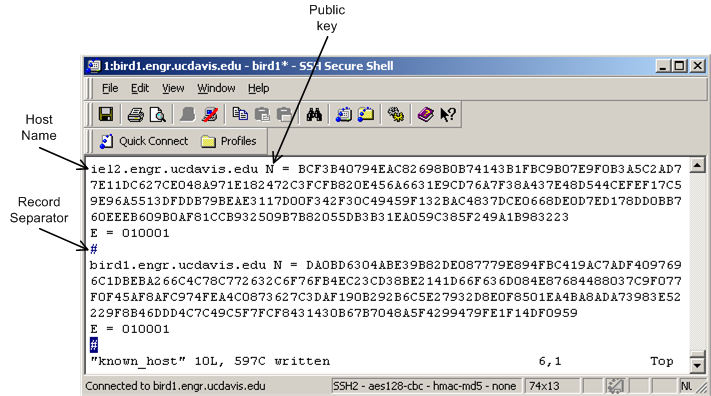
\includegraphics[scale=0.5]{figure/knownhost}
   \caption{A sample known host file.}
   \label{fig:knownhost}
\end{center}
\end{figure*}
% FIGURE }}}
%%%%%%%%%%%%%%%%%%%%%%%%%%%%%%%%%%%%%%%%%%%%%%%%%%%%%%%%%%%%%%%%%%%%%%

%%%%%%%%%%%%%%%%%%%%%%%%%%%%%%%%%%%%%%%%%%%%%%%%%%%%%%%%%%%%%%%%%%%%%%
% Known Host file {{{
\subsection{Known Host File}
After creating the key files for all the agencies in a network the 
  \textit{known\_host} file needs to be created manully.
The sample \textit{known\_host} file is shown in Figure ~\ref{fig:knownhost}. 
To proceed, create a file using a text editor with name 
  \textit{known\_host}. 
Type the name of the first agency (as shown \textit{Host Name} in 
Figure ~\ref{fig:knownhost}) and 
copy its public key from \textit{rsa\_pub} file. Insert the record 
separation character \# and type the same for second agency and continue.
Make sure that the name for the \textit{known\_host} file is 
\textit{``known\_host"}. After creating the 
\textit{known\_host} file, copy the \textit{known\_host} file to each \
agency and the \textit{rsa\_priv} file on the respective
agencies (the same directory from where you will run the Mobile-C 
agency). 
Public and private key files are always created as a pair this means that
  any text encrypted with the public key can only be decrypted with the
  corresponding (paired) private key.
Therefore, please make sure that the copied private key 
(\textit{rsa\_priv}) to an agency must correspond to the public key
that is mentioned infront of the name of this agency in \textit{
known\_host} file.
% }}} Known Host File
%%%%%%%%%%%%%%%%%%%%%%%%%%%%%%%%%%%%%%%%%%%%%%%%%%%%%%%%%%%%%%%%%%%%%%

%}}} Preparation to Run Security Enabled Agency
%%%%%%%%%%%%%%%%%%%%%%%%%%%%%%%%%%%%%%%%%%%%%%%%%%%%%%%%%%%%%%%%%%%%%

%%%%%%%%%%%%%%%%%%%%%%%%%%%%%%%%%%%%%%%%%%%%%%%%%%%%%%%%%%%%%%%%%%%%%
% Examples {{{
\section{Examples -- Mobile-C Security}
A Mobile-C security enable agency can be executed with encypted or plaintext
  private key. 
When you execute a Mobile-C agency it will look for private key file named
  \textit{rsa\_priv} in the current directory. 
If the private key is encrypted and the passphrase is not provided in Mobile-C
  agency C program then it will prompt for the passphrase.
\texttt{<MCPACKAGE>/demos/} contains two demos 
  (\textit{hello\_world\_secure} and \textit{multi\_task\_example\_secure}) that 
  uses private key in plain text.

Please note that for \textit{hello\_world\_secure} demo, the private and public
  key pair is same for client and server, that is both the client and server 
  program run on the same machine (iel2.engr.ucdavis.edu).
To run the demo in your machine, you to write the name of your machine in 
  \textit{known\_host} file and the mobile agent file (\textit{test1.xml}) 

To run client and server agencies on the two different machines, you need to
  create a pair of public and private keys (see section 9.3.1) and that 
  is for the second machine.  
The first agency can use the already created key files that are provided with
  demos.
After creating the key files, edit the \textit{known\_host} file by including
  the name of other machine and newly created public key from file 
  (\textit{rsa\_priv}), for details see section 9.3.2.
Also copy the newly generated private key file (\textit{rsa\_priv}) and 
  updated \textit{known\_host} file on the other machine in the same 
  directory from where Mobile-C agency will be executed.
Now start the server program and then the client program.

Please note that when you build the demos, the executable 
 files ( \textit{client} and  \textit{server}) for demo 
 \textit{hello\_world \_secure} are in 
 directories \textit{hello\_world\_secure/client} and 
 \textit{hello\_world\_ secure/server} respectively. Similarly, the executable 
 files (\textit{client},  \textit{server1} and  \textit{server2} ) for demo
  \textit{multi\_task\_example\_secure} are in directories 
   \textit{multi\_task\_e xample\_secure/client}, 
   \textit{multi\_task\_example\_secure/server1} and
   \textit{multi\_task\_example\_secure/server2} respectively.

Each agency uses a separate \textit{known\_host},
  public(\textit{rsa\_pub}) and private key {\textit{rsa\_priv} pair files. 

\begin{Program}[!t]
\begin{center}
   {\footnotesize \linespread{1.0} \verbatiminput{../demos/mobilec_security/hello_world_secure/server.c }}
\end{center}
\caption{ A sample server side code for security enable agency 
       (\textit{../demos/mobilec\_security/hello\_world\_secure/server.c})}
\label{prog:security_server}
\end{Program}

\begin{Program}[!t]
\begin{center}
   {\footnotesize \linespread{1.0} \verbatiminput{../demos/mobilec_security/hello_world_secure/client.c }}
\end{center}
\caption{ A sample client side code for security enable agency
        (\textit{../demos/mobilec\_security/hello\_world\_secure/client.c})}
\label{prog:security_client}
\end{Program}

The programs \ref{prog:security_server} and \ref{prog:security_client} show 
  \textit{hello\_world\_secure} server and client code respectively.
Please note that the \textit{MC\_AgencyOptions\_t} is required only if the 
  private key file is encrypted. 
Since both programs use the private key file (\textit{rsa\_priv}) in plaintext
  so \textit{MC\_AgencyOptions\_t} is NULL in \textit{MC\_Initialize} function.

If you generate the private key file (\textit{rsa\_priv}) in encrypted form 
   (see section 9.3.1) then the Mobile-C agency requires the same passphrase 
    to decrypt its private key that you have entered to encrypted this file.
In this case \textit{MC\_AgencyOptions\_t} should not be NULL. 
It is a possible that passphrase would not be privided in the code. 
That is, this code can be run if 
  \textit{strcpy(options.passphrase, "xxxx");} is commented out.
In this case, if the private key is encyrpted the Mobile-C agency
  would prompt to enter passphrase at startup otherwise not. 

%To run the these programs in your machine you need to replace 
%  \textit{rabbit.engr.ucdavis.edu} to your machine name in 
%  \textit{client.c}, \textit{test1.xml} and \textit{known\_host}
%  file.
%The \textit{test1.xml} is a hello world mobile agent. \
     

% }}} Example


%%%%%%%%%%%%%%%%%%%%%%%%%%%%%%%%%%%%%%%%%%%%%%%%%%%%%%%%%%%%%%%%%%%%%%

% }}} Mobile-C Security Module
%%%%%%%%%%%%%%%%%%%%%%%%%%%%%%%%%%%%%%%%%%%%%%%%%%%%%%%%%%%%%%%%%%%%%%

%%%%%%%%%%%%%%%%%%%%%%%%%%%%%%%%%%%%%%%%%%%%%%%%%%%%%%%%%%%%%%%%%%%%%%
%{{{Communication With Other FIPA Compliant Agent Systems
\chapter{Communication With Other FIPA Compliant Agent Systems}
This section provides some brief examples regarding communication
between Mobile-C and other FIPA compliant agent systems.
\subsection{Example: Receiving a message from a JADE agent}
The following section contains details regarding an example where a
Mobile-C agent receives a message from a JADE agent. This example is
included to provide a brief overview of how FIPA ACL communication
operates between Mobile-C agencies and JADE agencies.

\subsubsection{Start a Mobile-C Agency}
The first step in the example is to start a Mobile-C agency and a suitable
agent to wait for a message. An example agency which performs these tasks
may be found in the directory \texttt{<MCPACKAGE>/demos/ jade\_to\_mc\_example/}.
To start the agency, simply go to the directory and execute the server
with the command
\begin{verbatim}
./server
\end{verbatim}
The server will start and load the sample agent named ``mobagent1'' in one step,
which should produce the following output (or similar):
\begin{verbatim}
Mobile-C Started

MobileC > This is mobagent1 from the agency at port 5050.
Now, I am going to wait until I receive a message. Waiting...
\end{verbatim}

\subsubsection{Create a JADE container}
The next step is to start a JADE agency. Instructions on how to obtain and
install JADE may be found at the website \texttt{<http://jade.tilab.com>} .
Once JADE in installed, use the command
\begin{verbatim}
java jade.Boot -gui
\end{verbatim}
to start a JADE container. Note that the command may vary across systems depending
on your java distribution and system setup. This command should produce a window
similar to the following:

\begin{center}
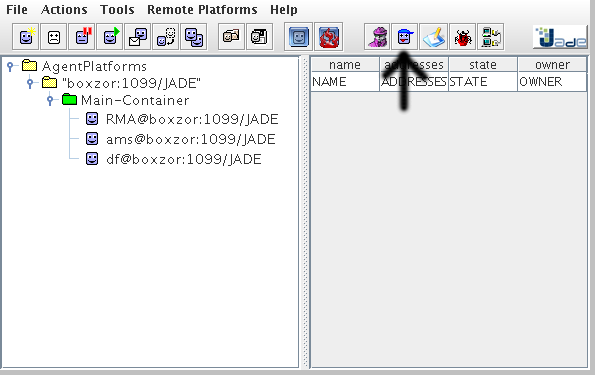
\includegraphics[width=4in]{figure/jade_to_mc_example/jade_main_window.png}
\end{center}

\subsubsection{Start a JADE dummy agent}
The next step is to start a ``dummy'' agent by clicking on the button indicated by the 
large arrow in the previous figure. This should produce a second window
which should resemble the following image.

\begin{center}
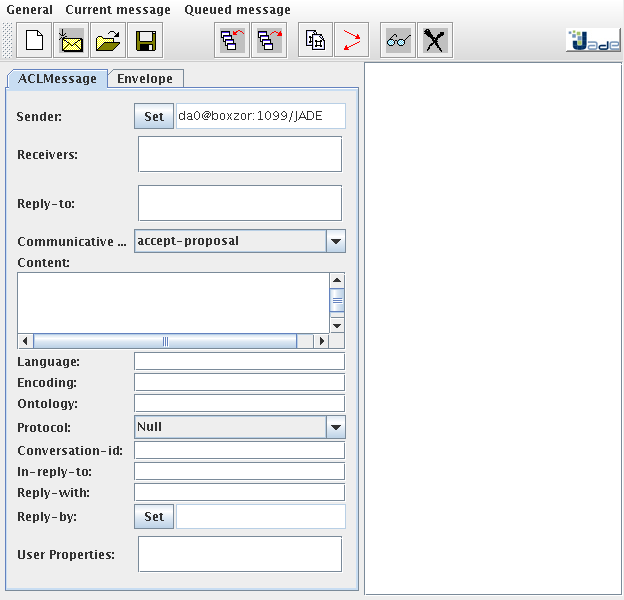
\includegraphics[width=4in]{figure/jade_to_mc_example/dummy_agent_window_blank.png}
\end{center}

\subsubsection{Send a message to Mobile-C}
There are several fields in this empty ACL message that need to be set before the
message will be successfully passed to our Mobile-C agent. The first field to fill
out is the \texttt{Receivers}, which indicates the recipients for our message.
We wish for our Mobile-C agent ``mobagent1'' to be our sole recipient. Add 
``mobagent1'' by right-clicking on the \texttt{Receivers} textbox and selecting the
\texttt{Add} option. Fill out the box as shown in the following image:

\begin{center}
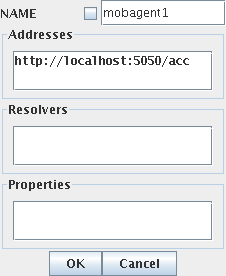
\includegraphics[width=2in]{figure/jade_to_mc_example/dummy_agent_receiver_window.png}
\end{center}

After setting the receiver, the rest of the message may be set to whatever is desired.
For this example, our sample message may be seen on the following image.

\begin{center}
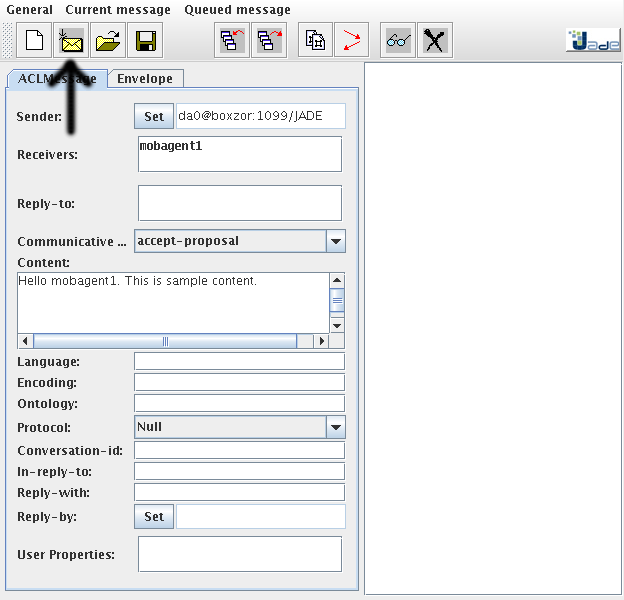
\includegraphics[width=4in]{figure/jade_to_mc_example/dummy_agent_window_complete.png}
\end{center}

Once your desired message parameters are in place, click on the ``Send Message'' button
indicated by the arrow in the previous figure. The message will be sent to the agent
waiting at the Mobile-C agency that was previously started. The agent should
receive the message and produce the following output:
\begin{verbatim}
mobagent1 Got a message!
Message is from da0@boxzor:1099/JADE
The content is Hello mobagent1. This is sample content.
\end{verbatim}
This indicates that \texttt{mobagent1} has successfully received the
message from JADE.

\subsection{Example: Sending a message from Mobile-C to JADE}
This example illustrates a Mobile-C agent sending an ACL message to a
JADE agent.  The example will be presented in a step by step fashion and all
files may be found in the directory \texttt{<MCPACKAGE>/demos/mc\_to\_jade\_example/}.

\subsubsection{Start a JADE container with a ``PingAgent'' agent}
The first step is to start a JADE container with a responsive agent. In this
example, we will use a demo ``PingAgent'' agent which is provided with JADE. The
agent source code may be found in the JADE subdirectory 
\texttt{jade/src/examples/PingAgent/PingAgent.java} . After installing JADE,
run the command
\begin{verbatim}
java jade.Boot pingme:examples.PingAgent.PingAgent
\end{verbatim}
from the \texttt{jade/src/} directory to start a JADE main container and 
invoke an agent of type ``PingAgent'' named ``pingme''. The ``PingAgent'' agent
contains a behaviour which receives messages and replies with a standard 
reply message. The ``PingAgent'' expects incoming messages to have a performative
of ``query-ref'', and for the content field to contain the text ``ping''. 

\subsubsection{Start a Mobile-C agency with a sender agent}
A Mobile-C agency and agent for use in the example has already been
created and reside in the directory \texttt{<MCPACKAGE>/demos/mc\_to\_jade\_example/} .
After compiling Mobile-C and the Mobile-C demos, simply go to the directory and
run the 'client' executable.
\begin{verbatim}
./client
\end{verbatim}
The executable will automatically start a Mobile-C agency and load an agent
named ``mobagent1''. The agent is programmed to send an ACL message to 
``pingme'' at the local JADE container and wait for a response message. 
Upon receiving the response, the agent will print the contents of the 
response message. The Mobile-C agent output should look something like
\begin{verbatim}
Mobile-C Started
Sending agent to self...
Done.
mobagent2 Creating new ACL message...
mobagent2 sending ACL message...
Received a message from pingme@boxzor:1099/JADE.
Content is 'alive'.
\end{verbatim}
%}}}
%%%%%%%%%%%%%%%%%%%%%%%%%%%%%%%%%%%%%%%%%%%%%%%%%%%%%%%%%%%%%%%%%%%%%%

%%%%%%%%%%%%%%%%%%%%%%%%%%%%%%%%%%%%%%%%%%%%%%%%%%%%%%%%%%%%%%%%%%%%%%
% Bibliography {{{
%\phantomsection
%\addcontentsline{toc}{chapter}{Bibliography}
\bibliographystyle{IEEEtran}
%\bibliography{/home/chgroup/project/paper/ielpaper}
\bibliography{ielpaper}
\pagebreak
% }}} Bibliography 
%%%%%%%%%%%%%%%%%%%%%%%%%%%%%%%%%%%%%%%%%%%%%%%%%%%%%%%%%%%%%%%%%%%%%%

%%%%%%%%%%%%%%%%%%%%%%%%%%%%%%%%%%%%%%%%%%%%%%%%%%%%%%%%%%%%%%%%%%%%%%
% Appendix {{{
\appendix
\chapter{Mobile-C API in the C/C++ Binary Space \label {appendix}}
\lhead{Mobile-C API in the C/C++ Binary Space}
\noindent
The header file {\bf libmc.h} defines all the data types, macros 
and function prototypes for the Mobile-C library.
The header file is used in the C/C++ binary space.

\begin{table}[!h]
\capstart
\begin{center}
\caption{Data types defined in {\bf libmc.h}.}
\begin{tabular}{p{50 mm}p{110 mm}}
\hline
Data Type & Description \\
\hline
{\bf MCAgency\_t} & A handle containing information of an agency. \\
{\bf MCAgent\_t} & A handle containing information of a mobile agent. \\
{\bf MCAgencyOptions\_t} & A structure containing information about which thread(s) to be activated and the default agent status specified by a user. \\
\hline
\end{tabular}
\end{center}
\label{mobilec_datatype}
\end{table}

The header file {\bf fipa\_acl.h} contains datatype and macros related to 
FIPA ACL messaging, as described in Chapter \ref{chap:fipa}. This header
file may be used in both C/C++ binary space, as well as agent space.

\begin{table}[!h]
\capstart
\begin{center}
\caption{Data types defined in {\bf fipa\_acl.h}.}
\begin{tabular}{p{50 mm}p{110 mm}}
\hline
Data Type & Description \\
\hline
{\bf fipa\_acl\_message\_t} & A structure containing a FIPA ACL message. \\
\hline
\end{tabular}
\end{center}
\label{fipa_datatype}
\end{table}

\pagebreak

\begin{table}[!h]
\capstart
\begin{center}
\caption{Macros defined in {\bf libmc.h}.}
\begin{tabular}{p{50 mm}p{110 mm}}
\hline
Macro & Description \\
\hline
{\texttt enum MC\_ThreadIndex\_e} & \\
\hline
{\bf MC\_THREAD\_AI} \index{MC\_THREAD\_AI} & Identifier for agent initalizing thread. \\
{\bf MC\_THREAD\_AM} \index{MC\_THREAD\_AM} & Identifier for agent managing thread. \\
{\bf MC\_THREAD\_CL} \index{MC\_THREAD\_CL} & Identifier for connection listening thread. \\
{\bf MC\_THREAD\_MR} \index{MC\_THREAD\_MR} & Identifier for message receiving thread. \\
{\bf MC\_THREAD\_MS} \index{MC\_THREAD\_MS} & Identifier for message sending thread. \\
{\bf MC\_THREAD\_CP} \index{MC\_THREAD\_CP} & Identifier for command prompt thread. \\
{\bf MC\_THREAD\_ALL} \index{MC\_THREAD\_ALL} & Identifier for all threads. \\
\hline
{\texttt enum MC\_Signal\_e} & \\
\hline
{\bf MC\_RECV\_CONNECTION} \index{MC\_RECV\_CONNECTION} & Signal activated after an agency accepts a connection. \\
{\bf MC\_RECV\_MESSAGE} \index{MC\_RECV\_MESSAGE} & Signal activated after an agency receives an ACL message. \\
{\bf MC\_RECV\_AGENT} \index{MC\_RECV\_AGENT} & Signal activated after an agency receives a mobile agent. \\
{\bf MC\_RECV\_RETURN} \index{MC\_RECV\_RETURN} & Signal activated after an agency receives return data from a completed mobile agent. \\
{\bf MC\_EXEC\_AGENT} \index{MC\_EXEC\_AGENT} & Signal activated after a mobile agent is executed. \\
{\bf MC\_ALL\_SIGNALS} \index{MC\_ALL\_SIGNALS} & Signal activated after any of the above four events occurs. \\
\hline
{\texttt enum MC\_AgentType\_e} \index{MC\_AgentType\_e}& \\
\hline
{\bf MC\_REMOTE\_AGENT} \index{MC\_REMOTE\_AGENT} & Identifier for a remote mobile agent. \\
{\bf MC\_LOCAL\_AGENT} \index{MC\_LOCAL\_AGENT} & Identifier for a local mobile agent.\\
{\bf MC\_RETURN\_AGENT} \index{MC\_RETURN\_AGENT} & Identifier for a return mobile agent. \\
\hline
{\texttt enum MC\_AgentStatus\_e} \index{MC\_AgentStatus\_e} & \\
\hline
{\bf MC\_WAIT\_CH} \index{MC\_WAIT\_CH} & Value indicating a mobile agent is waiting to be executed. \\
{\bf MC\_WAIT\_MESSGSEND} \index{MC\_WAIT\_MESSGSEND}& Value indicating a mobile agent is waiting to be exported to another agency. \\
{\bf MC\_AGENT\_ACTIVE} \index{MC\_AGENT\_ACTIVE}& Value indicating a mobile agent is being executed. \\
{\bf MC\_AGENT\_NEUTRAL} \index{MC\_AGENT\_NEUTRAL}& Value indicating a mobile agent is waiting for an unspecified reason. \\
{\bf MC\_AGENT\_SUSPENDED} \index{MC\_AGENT\_SUSPENDED}& Value indicating a mobile agent is being suspended. \\
{\bf MC\_WAIT\_FINISHED} \index{MC\_WAIT\_FINISHED}& Value indicating a mobile agent has been executed and is waiting to be removed. \\
\hline
\end{tabular}
\end{center}
\label{mobilec_macro}
\end{table}

\begin{table}[!hp]
\capstart
\begin{center}
\caption{Macros defined in {\bf fipa\_acl.h}. Detailed documentation for the
FIPA performatives and protocols may be found in the FIPA specifications at
\texttt{http://www.fipa.org}.}
\begin{tabular}{p{90 mm}p{70 mm}}
\hline
Macro & Description \\
\hline
{\texttt fipa\_performative\_e \index{fipa\_performative\_e}} & \\
\hline
{\bf FIPA\_ACCEPT\_PROPOSAL} \index{FIPA\_ACCEPT\_PROPOSAL} & The \texttt{accept-proposal} performative. \\
{\bf FIPA\_AGREE} \index{FIPA\_AGREE} & The \texttt{agree} performative. \\
{\bf FIPA\_CANCEL} \index{FIPA\_CANCEL} & The \texttt{cancel} performative. \\
{\bf FIPA\_CALL\_FOR\_PROPOSAL} \index{FIPA\_CALL\_FOR\_PROPOSAL} & The \texttt{call-for-proposal} performative. \\
{\bf FIPA\_CONFIRM} \index{FIPA\_CONFIRM} & The \texttt{confirm} performative. \\
{\bf FIPA\_DISCONFIRM} \index{FIPA\_DISCONFIRM} & The \texttt{disconfirm} performative. \\
{\bf FIPA\_FAILURE} \index{FIPA\_FAILURE} & The \texttt{failure} performative. \\
{\bf FIPA\_INFORM} \index{FIPA\_INFORM} & The \texttt{inform} performative. \\
{\bf FIPA\_INFORM\_IF} \index{FIPA\_INFORM\_IF} & The \texttt{inform-if} performative. \\
{\bf FIPA\_INFORM\_REF} \index{FIPA\_INFORM\_REF} & The \texttt{inform-ref} performative. \\
{\bf FIPA\_NOT\_UNDERSTOOD} \index{FIPA\_NOT\_UNDERSTOOD} & The \texttt{not-understood} performative. \\
{\bf FIPA\_PROPOGATE} \index{FIPA\_PROPOGATE} & The \texttt{propogate} performative. \\
{\bf FIPA\_PROPOSE} \index{FIPA\_PROPOSE} & The \texttt{propose} performative. \\
{\bf FIPA\_PROXY} \index{FIPA\_PROXY} & The \texttt{proxy} performative. \\
{\bf FIPA\_QUERY\_IF} \index{FIPA\_QUERY\_IF} & The \texttt{query-if} performative. \\
{\bf FIPA\_QUERY\_REF} \index{FIPA\_QUERY\_REF} & The \texttt{query-ref} performative. \\
{\bf FIPA\_REFUSE} \index{FIPA\_REFUSE} & The \texttt{refuse} performative. \\
{\bf FIPA\_REJECT\_PROPOSAL} \index{FIPA\_REJECT\_PROPOSAL} & The \texttt{reject-proposal} performative. \\
{\bf FIPA\_REQUEST} \index{FIPA\_REQUEST} & The \texttt{request} performative. \\
{\bf FIPA\_REQUEST\_WHEN} \index{FIPA\_REQUEST\_WHEN} & The \texttt{request-when} performative. \\
{\bf FIPA\_REQUEST\_WHENEVER} \index{FIPA\_REQUEST\_WHENEVER} & The \texttt{request-whenever} performative. \\
{\bf FIPA\_SUBSCRIBE} \index{FIPA\_SUBSCRIBE} & The \texttt{subscribe} performative. \\
\hline
{\texttt enum fipa\_protocol\_e} & \\
\hline
{\bf FIPA\_PROTOCOL\_REQUEST} \index{FIPA\_PROTOCOL\_REQUEST} & The FIPA \texttt{request} protocol. \\
{\bf FIPA\_PROTOCOL\_QUERY} \index{FIPA\_PROTOCOL\_QUERY} & The FIPA \texttt{query} protocol. \\
{\bf FIPA\_PROTOCOL\_REQUEST\_WHEN} \index{FIPA\_PROTOCOL\_REQUEST\_WHEN} & The FIPA \texttt{request-when} protocol. \\
{\bf FIPA\_PROTOCOL\_CONTRACT\_NET} \index{FIPA\_PROTOCOL\_CONTRACT\_NET} & The FIPA \texttt{contract-net} protocol. \\
{\bf FIPA\_PROTOCOL\_ITERATED\_CONTRACT\_NET} \index{FIPA\_PROTOCOL\_ITERATED\_CONTRACT\_NET} & The FIPA \texttt{iterated-contract-net} protocol. \\
{\bf FIPA\_PROTOCOL\_ENGLISH\_AUCTION} \index{FIPA\_PROTOCOL\_ENGLISH\_AUCTION} & The FIPA \texttt{english-auction} protocol. \\
{\bf FIPA\_PROTOCOL\_DUTCH\_AUCTION} \index{FIPA\_PROTOCOL\_DUTCH\_AUCTION} & The FIPA \texttt{dutch-auction} protocol. \\
{\bf FIPA\_PROTOCOL\_BROKERING} \index{FIPA\_PROTOCOL\_BROKERING} & The FIPA \texttt{brokering} protocol. \\
{\bf FIPA\_PROTOCOL\_RECRUITING} \index{FIPA\_PROTOCOL\_RECRUITING} & The FIPA \texttt{recruiting} protocol. \\
{\bf FIPA\_PROTOCOL\_SUBSCRIBE} \index{FIPA\_PROTOCOL\_SUBSCRIBE} & The FIPA \texttt{subscribe} protocol. \\
{\bf FIPA\_PROTOCOL\_PROPOSE} \index{FIPA\_PROTOCOL\_PROPOSE} & The FIPA \texttt{propose} protocol. \\
{\bf FIPA\_PROTOCOL\_END} \index{FIPA\_PROTOCOL\_END} & The FIPA \texttt{end} protocol. \\
\hline
\end{tabular}
\end{center}
\label{fipa_macro}
\end{table}

\begin{table}[!hp]
\capstart
\begin{center}
\caption{Functions in the C/C++ binary space.}
\begin{tabular}{p{78 mm}p{77 mm}}
%\begin{tabular}{ll}
\hline
Function & Description \\
\hline
{\bf MC\_AclAddReceiver()} \dotfill & Add a receiver to an ACL message. \\
{\bf MC\_AclAddReplyTo()} \dotfill & Add a reply-to address to an ACL message. \\
{\bf MC\_AclGetContent()} \dotfill & Get the content of an ACL message. \\
{\bf MC\_AclGetConversationID()} \dotfill & Get the conversation id from an ACL message. \\
{\bf MC\_AclGetPerformative()} \dotfill & Get the performative of an ACL message. \\
{\bf MC\_AclGetProtocol()} \dotfill & Get the protocol from an ACL message. \\
{\bf MC\_AclGetSender()} \dotfill & Get the sender of an ACL message. \\
{\bf MC\_AclNew()} \dotfill & Allocate a new FIPA ACL message. \\
{\bf MC\_AclPost()} \dotfill & Post a FIPA ACL message to an agent's mailbox. \\
{\bf MC\_AclReply()} \dotfill & Allocate a new FIPA ACL message automatically addressed to the sender of a previous message. \\
{\bf MC\_AclRetrieve()} \dotfill & Retrieve an ACL message from an agent's mailbox. \\
{\bf MC\_AclSetContent()} \dotfill & Set the content of an ACL message. \\
{\bf MC\_AclSetConversationID()} \dotfill & Set the conversation id of an ACL message. \\
{\bf MC\_AclSetPerformative()} \dotfill & Set the performative of an ACL message. \\
{\bf MC\_AclSetProtocol()} \dotfill & Set the protocol of an ACL message. \\
{\bf MC\_AclSetSender()} \dotfill & Set the sender of an ACL message. \\
{\bf MC\_AclWaitRetrieve()} \dotfill & Wait for a message to arrive at an agent's mailbox. \\
{\bf MC\_AgentAddTask()} \dotfill & Add a task to an agent based off of C source code. \\
{\bf MC\_AgentAddTaskFromFile()} \dotfill & Add a task to an agent based off of a C source code file. \\
{\bf MC\_AgentAttachFile()} \dotfill & Attach a file to the agent's current task. \\
{\bf MC\_AgentListFiles()} \dotfill & List files attached to an agent's task. \\
{\bf MC\_AgentRetrieveFile()} \dotfill & Retrieve and save an agent's attached file onto the filesystem. \\
{\bf MC\_AgentReturnArrayDim()} \dotfill & Get the dimension of an array returned by an agent. \\
{\bf MC\_AgentReturnArrayExtent()} \dotfill & Get the extent of a dimension of an array returned by an agent. \\
{\bf MC\_AgentReturnArrayNum()} \dotfill & Get the number of elements of an array returned by an agent. \\
{\bf MC\_AgentReturnDataGetSymbolAddr()} \dotfill & Get a pointer to an array returned by an agent. \\
{\bf MC\_AgentReturnDataSize()} \dotfill & Get the size of a single element of the array. \\
{\bf MC\_AgentReturnDataType()} \dotfill & Get the type of the array. \\
{\bf MC\_AgentReturnIsArray()} \dotfill & Determine if the returned variable is an array. \\
{\bf MC\_AddAgent()} \dotfill & Add a mobile agent into an agency. \\
{\bf MC\_AddAgentInitCallback()} \dotfill & Add an agent initialization callback function into an agency. \\
{\bf MC\_AddStationaryAgent()} \dotfill & Add a mobile agent into an agency. \\
%{\bf MC\_AgentVariableRetrieve()} & Retrieve a saved variable from an agent's prior task. \\
%{\bf MC\_AgentVariableSave()} & Save an agent's task variable for migration. \\
{\bf MC\_Barrier()} \dotfill & Block until all agents in an agency have called this function. \\
{\bf MC\_BarrierDelete()} \dotfill & Delete a Mobile-C barrier. \\
{\bf MC\_BarrierInit()} \dotfill & Initialize a Mobile-C barrier. \\
{\bf MC\_CallAgentFunc()} \dotfill & Call a function defined in an agent. \\
{\bf MC\_CallAgentFuncV()} \dotfill & Call a function defined in an agent. \\
\hline
\end{tabular}
\end{center}
\label{mobilec_api_cbinary}
\end{table}

\addtocounter{table}{-1}
\begin{table}[!hp]
\capstart
\begin{center}
\caption{Functions in the C/C++ binary space (contd.).}
%\begin{tabular}{ll}
\begin{tabular}{p{78 mm}p{77 mm}}
\hline
Function & Description \\
\hline
{\bf MC\_CallAgentFuncVar()} \dotfill & Call a function defined in an agent. \\
{\bf MC\_ChInitializeOptions()} \dotfill & Set the initialization options for a Ch to be used as one AEE in an agency. \\
{\bf MC\_ComposeAgent()} \dotfill & Compose an agent from program source code. \\
{\bf MC\_ComposeAgentS()} \dotfill & [Deprecated] Compose an agent from program source code with a workgroup code. \\
{\bf MC\_ComposeAgentWithWorkgroup()} \dotfill & Compose an agent from program source code with a workgroup code. \\
{\bf MC\_ComposeAgentFromFile()} \dotfill & Compose an agent from a program source code file. \\
{\bf MC\_ComposeAgentFromFileS()} \dotfill & [Deprecated] Compose an agent from a program source code file with a workgroup code. \\
{\bf MC\_ComposeAgentFromFileWithWorkgroup()} & Compose an agent from a program source code file with a workgroup code. \\
{\bf MC\_CondBroadcast()} \dotfill & Wake up all agents/threads waiting on a condition variable. \\
{\bf MC\_CondReset()} \dotfill & Reset a Mobile-C condition variable. \\
{\bf MC\_CondSignal()} \dotfill & Signal another agent that is waiting on a condition variable. \\
{\bf MC\_CondWait()} \dotfill & Cause the calling agent or thread to wait on a Mobile-C condition variable with the ID specified by the argument. \\
{\bf MC\_CopyAgent()} \dotfill & Perform a deep copy to copy an agent. \\
{\bf MC\_DeleteAgent()} \dotfill & Stop and remove an agent from an agency. \\
{\bf MC\_DeregisterService()} \dotfill & Deregister a service with the Directory Facilitator. \\
{\bf MC\_End()} \dotfill & Terminate a Mobile-C agency. \\
{\bf MC\_FindAgentByID()} \dotfill & Find a mobile agent by its ID number in an agency.\\
{\bf MC\_FindAgentByName()} \dotfill & Find a mobile agent by its name in an agency. \\
{\bf MC\_GetAgentArrivalTime()} \dotfill & Get the time when an agent arrives an agency. \\
{\bf MC\_GetAgentExecEngine()} \dotfill & Get the AEE associated with a mobile agent in an agency. \\
{\bf MC\_GetAgentID()} \dotfill & Get the ID of an agent. \\
{\bf MC\_GetAgentName()} \dotfill & Get the name of an agent. \\
{\bf MC\_GetAgentNumTasks()} \dotfill & Get the number of tasks a mobile agent has. \\
{\bf MC\_GetAgentReturnData()} \dotfill & [Deprecated] Get the return data of a mobile agent. \\
{\bf MC\_GetAgentStatus()} \dotfill & Get the status of a mobile agent in an agency. \\
{\bf MC\_GetAgentType()} \dotfill & Get the type of a mobile agent. \\
{\bf MC\_GetAgentXMLString()} \dotfill & Retrieve a mobile agent message in XML format as a character string. \\
{\bf MC\_GetAllAgents()} \dotfill & Obtain all the agents in an agency. \\
{\bf MC\_HaltAgency()} \dotfill & Halt an agency's operation. \\
{\bf MC\_Initialize()} \dotfill & Start a Mobile-C agency and return a handle of the launched agency. \\
{\bf MC\_InitializeAgencyOptions()} \dotfill & Initialize Mobile-C options. \\
{\bf MC\_LoadAgentFromFile()} \dotfill & Load an agent from an XML file into a local agency.\\
\hline
\end{tabular}
\end{center}
\end{table}
\pagebreak

\addtocounter{table}{-1}
\begin{table}[!hp]
\capstart
\begin{center}
\caption{Functions in the C/C++ binary space (contd.).}
%\begin{tabular}{ll}
\begin{tabular}{p{63 mm}p{97 mm}}
\hline
Function & Description \\
\hline
{\bf MC\_MainLoop()} \dotfill & Cause the calling thread to wait indefinitely on an agency.\\
{\bf MC\_MigrateAgent()} \dotfill & Migrate an agent. \\
{\bf MC\_MutexLock()} \dotfill & Lock a previously initialized Mobile-C synchronization variable as a mutex. \\
{\bf MC\_MutexUnlock()} \dotfill & Unlock a locked Mobile-C synchronization variable. \\
{\bf MC\_PrintAgentCode()} \dotfill & Print a mobile agent code for inspection. \\
{\bf MC\_RegisterService()} \dotfill &  Register a new service with the Directory Facilitator. \\
{\bf MC\_ResetSignal()} \dotfill &  Reset the Mobile-C signalling system. \\
{\bf MC\_ResumeAgency()} \dotfill &  Resume an agency's operation. \\
{\bf MC\_RetrieveAgent()} \dotfill & Retrieve the first neutral mobile agent from a mobile agent list. \\
{\bf MC\_RetrieveAgentCode()} \dotfill & Retrieve a mobile agent code in the form of a character string. \\
{\bf MC\_SearchForService()} \dotfill & Search the Directory Facilitator for a service. \\
{\bf MC\_SemaphorePost()} \dotfill & Unlock one resource from a Mobile-C semaphore. \\
{\bf MC\_SemaphoreWait()} \dotfill & Allocate one resource from a Mobile-C synchronization semaphore variable. \\
{\bf MC\_SendAgent()} \dotfill & Send an ACL mobile agent message to a remote agency. \\
{\bf MC\_SendAgentFile()} \dotfill & Send an ACL mobile agent message saved as a file to a remote agency. \\
{\bf MC\_SendAgentMigrationMessage()} \dotfill & [Deprecated] Send an ACL mobile agent message to a remote agency. \\
{\bf MC\_SendAgentMigrationMessageFile()} \dotfill & [Deprecated] Send an ACL mobile agent message saved as a file to a remote agency. \\
{\bf MC\_SendSteerCommand()} \dotfill & Send a command to control a steerable binary space function. \\
{\bf MC\_SetAgentStatus()} \dotfill & Set the status of a mobile agent in an agency. \\
{\bf MC\_SetDefaultAgentStatus()} \dotfill & Assign a user defined default status to all incoming mobile agents. \\
{\bf MC\_SetThreadOff()} \dotfill & Deactivate a thread in an agency. \\
{\bf MC\_SetThreadOn()} \dotfill & Activate a thread in an agency. \\
{\bf MC\_Steer()} \dotfill & Set up a steerable binary space function. \\
{\bf MC\_SteerControl()} \dotfill & Retrieve a steering command from the mobile agent space. \\
{\bf MC\_SyncDelete()} \dotfill & Delete a previously initialized synchronization variable. \\
{\bf MC\_SyncInit()} \dotfill & Initialize a new synchronization variable. \\
{\bf MC\_TerminateAgent()} \dotfill & Terminate the execution of a mobile agent in an agency. \\
%{\bf MC\_Wait()} \dotfill & Cause the calling thread to wait indefinitely on an agency.\\
{\bf MC\_WaitAgent()} \dotfill & Cause the calling thread to wait until a mobile agent is received. \\
{\bf MC\_WaitRetrieveAgent()} \dotfill & Block the calling thread until a mobile agent arrives, and return the mobile agent instead of executing it. \\
{\bf MC\_WaitSignal()} \dotfill & Block until one of the signals in the second argument is signalled.\\
\hline
\end{tabular}
\end{center}
\end{table}
\pagebreak

\newpage
\input{api/MC_AclGetProtocol}
\pagebreak
\input{api/MC_AclAddReceiver}
\pagebreak
\input{api/MC_AclAddReplyTo}
\pagebreak
\input{api/MC_AclGetContent}
\pagebreak
\input{api/MC_AclGetConversationID}
\pagebreak
\input{api/MC_AclGetPerformative}
\pagebreak
\input{api/MC_AclGetProtocol}
\pagebreak
\input{api/MC_AclGetSender}
\pagebreak
\input{api/MC_AclNew}
\pagebreak
\input{api/MC_AclPost}
\pagebreak
\input{api/MC_AclReply}
\pagebreak
\input{api/MC_AclRetrieve}
\pagebreak
\input{api/MC_AclSetContent}
\pagebreak
\input{api/MC_AclSetConversationID}
\pagebreak
\input{api/MC_AclSetPerformative}
\pagebreak
\input{api/MC_AclSetProtocol}
\pagebreak
\input{api/MC_AclSetSender}
\pagebreak
\input{api/MC_AclWaitRetrieve}
\pagebreak
\input{api/MC_AgentAddTask}
\pagebreak
\input{api/MC_AgentAddTaskFromFile}
\pagebreak
\input{api/MC_AgentAttachFile}
\pagebreak
\input{api/MC_AgentListFiles}
\pagebreak
\input{api/MC_AgentRetrieveFile}
\pagebreak
\input{api/MC_AgentReturnArrayDim}
\pagebreak
\input{api/MC_AgentReturnArrayExtent}
\pagebreak
\input{api/MC_AgentReturnArrayNum}
\pagebreak
\input{api/MC_AgentReturnDataGetSymbolAddr}
\pagebreak
\input{api/MC_AgentReturnDataSize}
\pagebreak
\input{api/MC_AgentReturnDataType}
\pagebreak
\input{api/MC_AgentReturnIsArray}
\pagebreak
\input{api/MC_AddAgent}
\pagebreak
\input{api/MC_AddAgentInitCallback}
\pagebreak
\input{api/MC_AddStationaryAgent}
\pagebreak
%\input{api/MC_AgentVariableRetrieve}
%\pagebreak
%\input{api/MC_AgentVariableSave}
%\pagebreak
\input{api/MC_Barrier}
\pagebreak
\input{api/MC_BarrierDelete}
\pagebreak
\input{api/MC_BarrierInit}
\pagebreak
\input{api/MC_CallAgentFunc}
\pagebreak
\input{api/MC_CallAgentFuncV}
\pagebreak
\input{api/MC_CallAgentFuncVar}
\pagebreak
\input{api/MC_ChInitializeOptions}
\pagebreak
\input{api/MC_ComposeAgent}
\pagebreak
\input{api/MC_ComposeAgentS}
\pagebreak
\input{api/MC_ComposeAgentWithWorkgroup}
\pagebreak
\input{api/MC_ComposeAgentFromFile}
\pagebreak
\input{api/MC_ComposeAgentFromFileS}
\pagebreak
\input{api/MC_ComposeAgentFromFileWithWorkgroup}
\pagebreak
\input{api/MC_CondBroadcast}
\pagebreak
\input{api/MC_CondReset}
\pagebreak
\input{api/MC_CondSignal}
\pagebreak
\input{api/MC_CondWait}
\pagebreak
\input{api/MC_CopyAgent}
\pagebreak
\input{api/MC_DeleteAgent}
\pagebreak
\input{api/MC_DeregisterService}
\pagebreak
\input{api/MC_End}
\pagebreak
\input{api/MC_FindAgentByID}
\pagebreak
\input{api/MC_FindAgentByName}
\pagebreak
\input{api/MC_GetAgentArrivalTime}
\pagebreak
\input{api/MC_GetAgentExecEngine}
\pagebreak
\input{api/MC_GetAgentID}
\pagebreak
\input{api/MC_GetAgentName}
\pagebreak
\input{api/MC_GetAgentNumTasks}
\pagebreak
\input{api/MC_GetAgentReturnData}
\pagebreak
\input{api/MC_GetAgentStatus}
\pagebreak
\input{api/MC_GetAgentType}
\pagebreak
\input{api/MC_GetAgentXMLString}
\pagebreak
\input{api/MC_GetAllAgents}
\pagebreak
\input{api/MC_HaltAgency}
\pagebreak
\input{api/MC_Initialize}
\pagebreak
\input{api/MC_InitializeAgencyOptions}
\pagebreak
\input{api/MC_LoadAgentFromFile}
\pagebreak
\input{api/MC_MainLoop}
\pagebreak
\input{api/MC_MigrateAgent}
\pagebreak
\input{api/MC_MutexLock}
\pagebreak
\input{api/MC_MutexUnlock}
\pagebreak
\input{api/MC_PrintAgentCode}
\pagebreak
\input{api/MC_RegisterService}
\pagebreak
\input{api/MC_ResetSignal}
\pagebreak
\input{api/MC_ResumeAgency}
\pagebreak
\input{api/MC_RetrieveAgent}
\pagebreak
\input{api/MC_RetrieveAgentCode}
\pagebreak
\input{api/MC_SearchForService}
\pagebreak
\input{api/MC_SemaphorePost}
\pagebreak
\input{api/MC_SemaphoreWait}
\pagebreak
\input{api/MC_SendAgent}
\pagebreak
\input{api/MC_SendAgentFile}
\pagebreak
\input{api/MC_SendAgentMigrationMessage}
\pagebreak
\input{api/MC_SendAgentMigrationMessageFile}
\pagebreak
\input{api/MC_SendSteerCommand}
\pagebreak
\input{api/MC_SetAgentStatus}
\pagebreak
\input{api/MC_SetDefaultAgentStatus}
\pagebreak
\input{api/MC_SetThreadOff}
\pagebreak
\input{api/MC_SetThreadOn}
\pagebreak
\input{api/MC_Steer}
\pagebreak
\input{api/MC_SteerControl}
\pagebreak
\input{api/MC_SyncDelete}
\pagebreak
\input{api/MC_SyncInit}
\pagebreak
\input{api/MC_TerminateAgent}
\pagebreak
%\input{api/MC_Wait}
%\pagebreak
\input{api/MC_WaitAgent}
\pagebreak
\input{api/MC_WaitRetrieveAgent}
\pagebreak
\input{api/MC_WaitSignal}
\pagebreak


\chapter{Mobile-C API in the C/C++ Script Space \label {appendixb}}
% Mobile-C Library 

%%%%%%%%%%%%%%%%%%%%%%%%%%%%%%%%%%%%%%%%%%%%%%%%%%%%%%%%%%%%%%%%%%%%%%
% Preamble {{{
%\documentclass[11pt]{article}
\documentclass[11pt]{report}
\usepackage{varioref}
\usepackage{times,here,verbatim,fancyheadings,makeidx}
%\usepackage{psfig}
\usepackage[pdftex]{hyperref}
\usepackage{hypcap}
\usepackage{fullpage}
\usepackage{amssymb,amsmath}
\usepackage{graphicx}
\usepackage{program}
\headrulewidth 0.0pt
\hoffset=-0.0625in
%\voffset=0pt
\setlength{\textheight}{9in}
\setlength{\textwidth}{6.5in}
\topmargin=0.05in
\makeindex
% }}} Preamble
%%%%%%%%%%%%%%%%%%%%%%%%%%%%%%%%%%%%%%%%%%%%%%%%%%%%%%%%%%%%%%%%%%%%%%

%%%%%%%%%%%%%%%%%%%%%%%%%%%%%%%%%%%%%%%%%%%%%%%%%%%%%%%%%%%%%%%%%%%%%%
% Title Page {{{
\begin{document}
\thispagestyle{empty}
\begin{center}

\includegraphics[width=1.8in]{figure/mobilec_logo.png}


\vspace{0.5in}
{\Huge\sf\bf Mobile-C} \\
\vspace{0.1in}
{\LARGE\sf\bf -- A Multi-Agent Platform for Mobile C/C++ Agents} \\
\vspace{0.4in}
{\LARGE\sf\bf User's Guide} \\
\vspace{0.4in}
{\LARGE\sf\bf Version 2.1.3} \\
\vspace{1.0in}
{\Large\sf\bf Harry H. Cheng} \\
\vspace{1.0in}
{\large\sf\bf Mobile-C User's Guide version 2.1.3 prepared by:} \\
\vspace{0.2in}
David Ko\\
Harry H. Cheng
\vspace{1in}

\vspace{2.0in}
{\large\sf\bf\today}
%September 20, 2007
\end{center}

%%%%%%%%%%%%%%%%%%%%%%%%%%%%%%%%%%%%%%%%%%%%%%%%%%%%%%%%%%%%%%%%%%%%%%
% Contributors {{{
%\phantomsection
%\addcontentsline{toc}{chapter}{Major contributors}
\pagebreak
\noindent
{\LARGE\sf\bf Major Contributors (in alphabetical order)} \\
{\small
\verbatiminput{../AUTHORS}
}
% }}} Contributors 
%%%%%%%%%%%%%%%%%%%%%%%%%%%%%%%%%%%%%%%%%%%%%%%%%%%%%%%%%%%%%%%%%%%%%%
\pagebreak


%%%%%%%%%%%%%%%%%%%%%%%%%%%%%%%%%%%%%%%%%%%%%%%%%%%%%%%%%%%%%%%%%%%%%%
% Copyright {{{
\thispagestyle{empty}
%\phantomsection
%\addcontentsline{toc}{chapter}{Copyright}
\noindent
{\Large\bf Copyright}\\
\verbatiminput{../Copyright}
% }}} Copyright 
%%%%%%%%%%%%%%%%%%%%%%%%%%%%%%%%%%%%%%%%%%%%%%%%%%%%%%%%%%%%%%%%%%%%%%

\pagebreak
% }}} Title Page
%%%%%%%%%%%%%%%%%%%%%%%%%%%%%%%%%%%%%%%%%%%%%%%%%%%%%%%%%%%%%%%%%%%%%%

%%%%%%%%%%%%%%%%%%%%%%%%%%%%%%%%%%%%%%%%%%%%%%%%%%%%%%%%%%%%%%%%%%%%%%
% Abstract {{{
%\phantomsection
%\addcontentsline{toc}{chapter}{Abstract}
\begin{abstract} 
Mobile-C is an IEEE FIPA (Foundation for Intelligent Physical Agents) standard 
compliant multi-agent platform for supporting C/C++ mobile agents in networked 
intelligent mechatronic and embedded systems. Although it is a general-purpose 
multi-agent platform, Mobile-C is specifically designed for real-time and 
resource constrained applications with interface to hardware. Mobile agents 
are software components that are able to move between different execution 
environments. Mobile agents in a multi-agent system communicate and work 
collaboratively with other agents to achieve a global goal. It allows a 
mechatronic or embedded system to adapt to a dynamically changing environment.

\vspace{1in}
%%%%%%%%%%%%%%%%%%%% begin figure %%%%%%%%%%%%%%%%%%%% 
%\begin{figure}[H]
\centerline{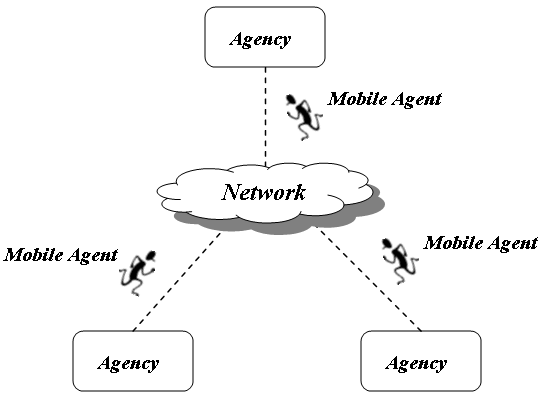
\includegraphics[scale=0.6]{figure/coverfigure}}
%\end{figure}
%%%%%%%%%%%%%%%%%%%% end figure %%%%%%%%%%%%%%%%%%%%%%
\end{abstract}
\pagebreak
% Abstract }}}
%%%%%%%%%%%%%%%%%%%%%%%%%%%%%%%%%%%%%%%%%%%%%%%%%%%%%%%%%%%%%%%%%%%%%%

%%%%%%%%%%%%%%%%%%%%%%%%%%%%%%%%%%%%%%%%%%%%%%%%%%%%%%%%%%%%%%%%%%%%%%
% Table of Contents {{{
\pagenumbering{roman}
\setcounter{page}{1}
\tableofcontents
\pagebreak
% }}} Table of Contents
%%%%%%%%%%%%%%%%%%%%%%%%%%%%%%%%%%%%%%%%%%%%%%%%%%%%%%%%%%%%%%%%%%%%%%

%%%%%%%%%%%%%%%%%%%%%%%%%%%%%%%%%%%%%%%%%%%%%%%%%%%%%%%%%%%%%%%%%%%%%%
% Part 1 {{{
\pagenumbering{arabic}
\setcounter{page}{1}
\pagebreak
% }}} Part 1 
%%%%%%%%%%%%%%%%%%%%%%%%%%%%%%%%%%%%%%%%%%%%%%%%%%%%%%%%%%%%%%%%%%%%%%

%%%%%%%%%%%%%%%%%%%%%%%%%%%%%%%%%%%%%%%%%%%%%%%%%%%%%%%%%%%%%%%%%%%%%%
% Introduction {{{
%\pagenumbering{arabic}
%\setcounter{page}{1}
%\pagestyle{fancy}
\chapter{Introduction}
Parallel and distributed computing~\cite{Kumar}~\cite{Manber} are widely used 
in scientific and engineering fields, especially for time-critical or 
time-consuming tasks.
Parallel computing is typically carried out in dedicated multiprocessors with
a central clock and shared memory.
On the other hand, distributed computing is decentralized parallel
computing, using two or more computers communicating over a network to
accomplish a common objective or task.
It is similar to computer clustering with the main difference being a wide
geographic dispersion of the resources.
In addition to the main difference, the types of hardware, programming 
languages, operating systems and other resources may vary drastically as well 
in distributed computing.

Although the processing speed of networked computers is typically not as fast 
as that of a dedicated parallel computer, networked computers are less
expensive and more broadly available.
Due to the rapid improvement in network hardware and software that makes
distributed computing faster, more broadly available, and easier-to-implement
than before, there are more and more research investigations nowadays 
targeting or exploiting this low-end, decentralized parallel computing.
Meanwhile, as the scale of distributed applications rapidly expands, 
there is an increasing demand for the code mobility.

Agent technology can significantly enhance the design and analysis of 
problem domains under the following three conditions~\cite{Adler}: 
(1) the problem domain is geographically distributed; 
(2) the subsystems exist in a dynamic environment; 
(3) the subsystems need to interact with each other more flexibly. 
Mobile agents are software components that can travel between 
different execution environments~\cite{Fuggetta}. 
Mobile agents can be created dynamically during runtime and dispatched to 
source systems to perform tasks with the most updated code. 
Therefore, the mobility of mobile agents provides distributed 
applications with significant flexibility and adaptability which are both 
essential to satisfy the dynamically changing requirements and conditions in 
a distributed environment.

Most of the mobile agent systems were developed to support only Java mobile 
agents.
Furthermore, many of them are standalone platforms. 
In other words, they were not designed to be embedded in a user application 
to support code mobility.  
Mobile-C~\cite{Chenthesis}~\cite{Chen3}~\cite{Mobile-C}~\cite{mobilec_webpage} 
was originally developed as a standalone, IEEE Foundation for Intelligent 
Physical Agents (FIPA) compliant mobile agent platform with a primary 
intention to fit applications where low-level hardware gets involved, such as 
networked mechatronic and embedded systems. 
Since most of these systems are written in C/C++, Mobile-C uses C/C++ as 
the mobile agent language for easy interfacing with control programs and 
underlying hardware. 
In addition, Mobile-C uses an embeddable C/C++ interpreter -- Ch, originally 
developed by Cheng~\cite{SP1}~\cite{CUJ1}~\cite{Ch}, to support the execution 
of C/C++ mobile agent code. 

In order to provide distributed applications with code mobility, this 
user's guide presents a mobile agent library, the Mobile-C library. 
The Mobile-C library is supported in various operating systems including 
Windows, Unix, and real-time OS.
It has a small footprint to satisfy the small memory requirement for a 
variety of mechatronic and embedded systems. 
This mobile agent library allows Mobile-C to be embedded in a program to 
support C/C++ mobile agents.
The API functions in this library facilitate the development of a multi-agent
system that can easily interface with a variety of hardware devices. 
%\pagebreak
% }}} Introduction
%%%%%%%%%%%%%%%%%%%%%%%%%%%%%%%%%%%%%%%%%%%%%%%%%%%%%%%%%%%%%%%%%%%%%%

%%%%%%%%%%%%%%%%%%%%%%%%%%%%%%%%%%%%%%%%%%%%%%%%%%%%%%%%%%%%%%%%%%%%%%
% Mobile-C Library Installation {{{
\chapter{Mobile-C Library Installation}
This chapter describes the prerequisites to install the Mobile-C library and 
the installation steps for both Unix and Windows operating systems.

%%%%%%%%%%%%%%%%%%%%%%%%%%%%%%%%%%%%%%%%%%%%%%%%%%%%%%%%%%%%%%%%%%%%%%
% SUB: Requirements {{{
\section{Requirements}
This user's guide assumes all necessary software packages are installed
correctly and function. 
The software packages required to successfully install the Mobile-C library 
include:

\noindent
(1) Ch version 6.3.0 or greater: It can be obtained from http://www.softintegration.com

\noindent
(2) Embedded Ch version 6.3.0 or greater: It can be obtained from http://www.softintegration.com

% }}} SUB: Prerequisites 
%%%%%%%%%%%%%%%%%%%%%%%%%%%%%%%%%%%%%%%%%%%%%%%%%%%%%%%%%%%%%%%%%%%%%%

%%%%%%%%%%%%%%%%%%%%%%%%%%%%%%%%%%%%%%%%%%%%%%%%%%%%%%%%%%%%%%%%%%%%%%
% SUB: Installation on Unix {{{
\section{Installation on Unix}

\subsection{Install the Mobile-C library}
The following commands will install the Mobile-C library in the system 
directory for {\bf 32-bit} Unix systems. 
The system directory for Unix systems is usually `/usr/local/lib' or 
  `/usr/lib' depending on your system.

\begin{verbatim}
    cd <MCPACKAGE>/src
    ./configure
    make
    make install
\end{verbatim}

The following commands will install the Mobile-C library in the system 
  directory for {\bf 64-bit} Unix systems. 
The only difference between the above and below commands is that `fPIC' is 
  added into CFLAGS for compilation.

\begin{verbatim}
    cd <MCPACKAGE>/src
    ./configure CFLAGS=-fPIC
    make
    make install
\end{verbatim}

By default, the Mobile-C library created contains both shared and static 
versions, which are `libmc.so.0.0.0' and `libmc.a', respectively.
The header file, libmc.h, used in the C/C++ binary 
space will be placed in the system directory, which is usually 
`usr/local/include' or `/usr/include' depending on your system.
 
Note that these commands will automatically build mxml-2.2.2 and
xyssl-0.7, both of which are packaged with Mobile-C, but will
not install these libraries. The Mobile-C libraries only need
these libraries to compile, but does not need them installed in
order to run.

Also note that the above commands will automatically compile all the included
demos automatically after compiling the Mobile-C library. The demos will
run even if the 'make install' step is omitted.

The `--prefix' option can be used to specify the home directory to 
install the Mobile-C files, as shown in the following commands.

\begin{verbatim}
    cd <MCPACKAGE>/src
    ./configure --prefix=<MCHOME>
    make
    make install
\end{verbatim}

\noindent
\texttt{<MCPACKAGE>} is the directory created by unpacking the Mobile-C compressed 
tar file.
\texttt{<MCHOME>} is the installation directory for the Mobile-C library and 
header file.\\
\noindent
The library files `libmc.so.0.0.0' and `libmc.a' will be installed in 
\texttt{<MCHOME>/lib}, and the header file `libmc.h' will be placed in 
\texttt{<MCHOME>/include}.

% }}} SUB: Installation on Unix
%%%%%%%%%%%%%%%%%%%%%%%%%%%%%%%%%%%%%%%%%%%%%%%%%%%%%%%%%%%%%%%%%%%%%%

%%%%%%%%%%%%%%%%%%%%%%%%%%%%%%%%%%%%%%%%%%%%%%%%%%%%%%%%%%%%%%%%%%%%%%
% SUB: Installation on Windows {{{
\section{Installation on Windows}
\subsection{Building the Mobile-C Library}
The following steps are suggested to build the Mobile-C library.
\begin{enumerate}
\item Ensure that your \texttt{\_chrc} file in your home directory is up to
  date. The \texttt{\_chrc} file may be opened from the ChIDE text editor by
  opening ChIDE, selecting "Options" from the menu, and selecting the "Open
  Local Ch Startup File" menu item. The section in your \texttt{\_chrc} file
  which contains settings about
  your Visual C++ installation must be correct. 
\item Unpack the Mobile-C source code. Ensure that you have write permissions
  for the directory you are unpacking Mobile-C into, or you may encounter 
  compile-time errors. As mentioned in the previous section, we will refer
  to the unpacked directory as \texttt{<MCPACKAGE>}.
\item Open a Ch terminal.
\item Navigate to the \texttt{<MCPACKAGE>} directory in your Ch terminal. For
  example, if you unpacked Mobile-C to the \texttt{C:$\backslash$Mobile-C} directory, type
  \texttt{cd C:$\backslash$Mobile-C} in your Ch terminal.
\item Type the command \texttt{nmake -f makefile.win32} to build the Mobile-C
  library, as well as all of the demos in the \texttt{<MCPACKAGE>/demos/}
  directory.
\end{enumerate}
% }}} SUB: Installation on Windows 
%%%%%%%%%%%%%%%%%%%%%%%%%%%%%%%%%%%%%%%%%%%%%%%%%%%%%%%%%%%%%%%%%%%%%%

%%%%%%%%%%%%%%%%%%%%%%%%%%%%%%%%%%%%%%%%%%%%%%%%%%%%%%%%%%%%%%%%%%%%%%
% SUB: Installation on KoreBot {{{
\section{Installation on KoreBot}

\subsection{Build the Mobile-C library}
A bash script, \textit{build\_korebot}, is used to build the Mobile-C library 
and an executable sample program, \textit{mc\_sample\_app}, for KoreBot board.

Running the script will create a directory called \textit{korebot\_mc} that 
contains \textit{bin}, \textit{include} and \textit{lib} directories.
\textit{bin} directory contains the executable sample program.    
\textit{include} directory contains the header file \textit{libmc.h}.
\textit{lib} directory contains the Mobile-C related static and shared 
libraries.

Two paths, \textit{KOREBOT\_CHHOME} and \textit{KOREBOT\_TOOLCHAINHOME}, 
in the bash script might need to be changed to match the correct 
paths set up in a user's system.
\textit{KOREBOT\_CHHOME} is the directory containing Ch files built for 
KoreBot board.
\textit{KOREBOT\_TOOLCHAINHOME} is the directory containing cross compiler 
related files for KoreBot board. 

Use the following commands to run the bash script.

\begin{verbatim}
    cd <MCPACKAGE>
    ./build_korebot
\end{verbatim}
% }}} SUB: Installation on KoreBot 
%%%%%%%%%%%%%%%%%%%%%%%%%%%%%%%%%%%%%%%%%%%%%%%%%%%%%%%%%%%%%%%%%%%%%%

%%%%%%%%%%%%%%%%%%%%%%%%%%%%%%%%%%%%%%%%%%%%%%%%%%%%%%%%%%%%%%%%%%%%%%
% SUB: Installation on Gumstix {{{
\section{Installation on Gumstix}

\subsection{Build the Mobile-C library}
A bash script, \textit{build\_gumstix}, is used to build the Mobile-C library 
and an executable sample program, \textit{mc\_sample\_app}, for Gumstix 
computer.

Running the script will create a directory called \textit{gumstix\_mc} that 
contains \textit{bin}, \textit{include} and \textit{lib} directories.
\textit{bin} directory contains the executable sample program.    
\textit{include} directory contains the header file \textit{libmc.h}.
\textit{lib} directory contains the Mobile-C related static and shared 
libraries.

Two paths, \textit{GUMSTIX\_CHHOME} and \textit{GUMSTIX\_TOOLCHAINHOME}, 
in the bash script might need to be changed to match the correct 
paths set up in a user's system.
\textit{GUMSTIX\_CHHOME} is the directory containing Ch files built for 
Gumstix computer. By default, it is set to the value \texttt{/usr/local/gumstix\_ch/ch/}.
\textit{GUMSTIX\_TOOLCHAINHOME} is the directory containing cross compiler 
related files for Gumstix computer. By default, it is set to the value \texttt{/usr/local/gumstix-buildroot}.

Use the following commands to run the bash script.

\begin{verbatim}
    cd <MCPACKAGE>
    ./build_gumstix
\end{verbatim}
% }}} SUB: Installation on Gumstix 
%%%%%%%%%%%%%%%%%%%%%%%%%%%%%%%%%%%%%%%%%%%%%%%%%%%%%%%%%%%%%%%%%%%%%%

%%%%%%%%%%%%%%%%%%%%%%%%%%%%%%%%%%%%%%%%%%%%%%%%%%%%%%%%%%%%%%%%%%%%%%
% Installing the Mobile-C Ch Package{{{
\section{Installing the Mobile-C Ch Package}
The Mobile-C Ch Package will be required if agents need to use any of the
Mobile-C FIPA ACL message functions, such as \texttt{mc\_AclSend()} or
\texttt{mc\_AclRetrieve()}. To install the Mobile-C Ch package, please follow
these steps:
\begin{enumerate}
\item From the Mobile-C root directory, run the command: \\
\texttt{ch ./pkgcreate.ch} \\
This will create a directory called ``\texttt{chmobilec}''.
\item From within a Ch shell, run the command: \\
\texttt{sudo pkginstall.ch chmobilec} \\
If you are using Microsoft Windows, you may omit the "\texttt{sudo}" part of the
command which is required on unix-like systems to ensure proper installation
permassions.
\end{enumerate}
% }}} Installing the Mobile-C Security Module
%%%%%%%%%%%%%%%%%%%%%%%%%%%%%%%%%%%%%%%%%%%%%%%%%%%%%%%%%%%%%%%%%%%%%%

\section{Creating your own compilation environment}
If a custom build environment is required, there are several directories which
must be added to the search paths for header files and libraries. There are 
also a variety of system libraries which Mobile-C must be linked with in order
to compile properly.

\subsection{UNIX and Mac systems}
In order to compile properly, the extra include directory
\texttt{<CHHOME>/extern/include} must be added to the default include search
directories. The directory \texttt{<CHHOME>/extern/lib} must also be added to
the list of searched library directories. Furthermore, the following libraries
must be linked with Mobile-C during the link step:
\begin{itemize}
\item libmxml (Provided with Mobile-C in the directory \texttt{<MCHOME>/src/mxml/})
\item libmc\_list (Provided with Mobile-C in the directory \texttt{<MCCHOME>/src/mc\_list})
\item libmc\_sync (Provided with Mobile-C in the directory \texttt{<MCCHOME>/src/mc\_sync})
\item libdl
\item libpthread
\item libm
\item libcrypt
\item libembedch (Provided with Embedded-Ch)
\end{itemize}

\subsection{Windows}
For windows, the include directory \texttt{<CHHOME>/extern/include} must be added
to the include paths and the directory \texttt{<CHHOME>/extern/lib} must be added
to the library search paths. Furthermore, the library \texttt{wsock32.lib} must
be linked with Mobile-C in order to compile properly.

% }}} Mobile-C Library Installation 
%%%%%%%%%%%%%%%%%%%%%%%%%%%%%%%%%%%%%%%%%%%%%%%%%%%%%%%%%%%%%%%%%%%%%%

%%%%%%%%%%%%%%%%%%%%%%%%%%%%%%%%%%%%%%%%%%%%%%%%%%%%%%%%%%%%%%%%%%%%%%
% Getting Started{{{
\chapter{Getting Started}
%%%%%%%%%%%%%%%%%%%%%%%%%%%%%%%%%%%%%%%%%%%%%%%%%%%%%%%%%%%%%%%%%%%%%%
% SUB: Compilation on Unix{{{
\section{Compilation on Unix}
All the demo programs are compiled automatically in the Unix version.
% }}} Compilation on Unix
%%%%%%%%%%%%%%%%%%%%%%%%%%%%%%%%%%%%%%%%%%%%%%%%%%%%%%%%%%%%%%%%%%%%%%

%%%%%%%%%%%%%%%%%%%%%%%%%%%%%%%%%%%%%%%%%%%%%%%%%%%%%%%%%%%%%%%%%%%%%%
% SUB: Compilation on Windows{{{
\section{Compilation on Windows}
All the demo programs are compiled automatically in the Windows version. Single
demos may be recompiled by navigating to a demo directory in a Ch terminal with
the \texttt{cd} and \texttt{ls} commands, and then executing the commands
\texttt{nmake -f makefile.win32} to compile a demo, or \texttt{nmake -f
makefile.win32 clean} to delete all compiled files.
% }}} SUB: Compilation on Windows 
%%%%%%%%%%%%%%%%%%%%%%%%%%%%%%%%%%%%%%%%%%%%%%%%%%%%%%%%%%%%%%%%%%%%%%

%%%%%%%%%%%%%%%%%%%%%%%%%%%%%%%%%%%%%%%%%%%%%%%%%%%%%%%%%%%%%%%%%%%%%%
% SUB: Overview of Sample Application Programs {{{
\section{Overview of Sample Application Programs}
%%%%%%%%%%%%%%%%%%%%%%%%%%%%%%%%%%%%%%%%%%%%%%%%%%%%%%%%%%%%%%%%%%%%%%
% Program: server.c {{{
\begin{Program}[!h]
\capstart
\begin{center}
   {\footnotesize \linespread{1.0} \verbatiminput{../demos/getting_started/hello_world/server.c}}
\end{center}
\caption{A sample Mobile-C server. (demos/getting\_started/hello\_world/server.c)}
\label{prog:server.c}
\end{Program}
% }}} Program: server.c
%%%%%%%%%%%%%%%%%%%%%%%%%%%%%%%%%%%%%%%%%%%%%%%%%%%%%%%%%%%%%%%%%%%%%%

%%%%%%%%%%%%%%%%%%%%%%%%%%%%%%%%%%%%%%%%%%%%%%%%%%%%%%%%%%%%%%%%%%%%%%
% Program: client.c {{{
\begin{Program}%[!h]
\capstart
\begin{center}
   {\footnotesize \linespread{1.0} \verbatiminput{../demos/getting_started/hello_world/client.c}}
\end{center}
\caption{A sample Mobile-C client program. The sole purpose of this program is to
  send a Mobile-C agent to another agency. (demos/getting\_started/hello\_world/client.c)}
\label{prog:client.c}
\end{Program}
% }}} Program: client.c
%%%%%%%%%%%%%%%%%%%%%%%%%%%%%%%%%%%%%%%%%%%%%%%%%%%%%%%%%%%%%%%%%%%%%%


Program \vref{prog:server.c} starts an agency that is capable of 
receiving mobile agents and executing mobile agent code. 

{\footnotesize \linespread{1.0} \verbatiminput{../demos/getting_started/hello_world/server.c.1}}
\noindent
The header file {\bf libmc.h} is included at the beginning of the program. 
It defines all the data types, macros and function prototypes for the 
Mobile-C library.

{\footnotesize \linespread{1.0} \verbatiminput{../demos/getting_started/hello_world/server.c.2}}
\noindent
The variable $agency$, of type {\bf MCAgency\_t}, is a handle that contains 
information of an agency. The second line initializes a local variable that will
hold the port number we wish the agency to bind to.

{\footnotesize \linespread{1.0} \verbatiminput{../demos/getting_started/hello_world/server.c.3}}
\noindent
{\bf MC\_Initialize()} \index{MC\_Initialize()} takes an integer and the address of an 
{\bf MCAgencyOptions\_t} \index{MCAgencyOptions\_t} variable as its two parameters. 
An {\bf MCAgencyOptions\_t} variable is a structure that contains 
information about which threads to be activated and the default agent 
status specified by a user.
Here, a {\bf NULL} pointer is passed to {\bf MC\_Initialize()} as the second 
parameter instead of an MCAgencyOptions\_t variable to start an agency with 
default settings. 
A local agency will be initialized to listen on port {\bf 5051} specified by 
the variable $local\_port$.

{\footnotesize \linespread{1.0} \verbatiminput{../demos/getting_started/hello_world/server.c.4}}
\noindent
The agency waits indefinitely for a mobile agent by the function 
{\bf MC\_MainLoop()} \index{MC\_MainLoop()}. 

Program \ref{prog:client.c} starts an agency that sends a mobile agent to 
a remote agency.
Examining Programs \ref{prog:server.c} and \ref{prog:client.c}, we see
that there are only two new API function calls:
\begin{verbatim}
  agent = MC_ComposeAgentFromFile(
      "mobagent1",      /* Name */
      "localhost:5050", /* Home */
      "IEL",            /* Owner */
      "hello_world.c",  /* Filename */
      NULL,             /* Return var name. NULL for no return */
      "localhost:5051", /* Server to execute task on */
      0 );              /* Persistent. 0 for no persistence. */
\end{verbatim}
and
\begin{verbatim}
  MC_AddAgent(agency, agent);
\end{verbatim}

Mobile-C agents may be created from existing source code files. The example
above takes a source code file called \texttt{hello\_world.c} and constructs
an agent around it. The agent's name, home, owner, return variable name,
and the host on which to execute the agent are all provided as arguments
to the \texttt{MC\_ComposeAgentFromFile()} function. 

Then, the newly created agent is added to the local agency so that it may
perform its local and/or remote tasks. In our example, the agent has
one remote task, so the agent will migrate to the remote host and perform
its task there. 

Also note that any valid hostname may be used in place of ``localhost''. The
communicating agencies need not be on the same physical machine; in fact, in most
cases they will be on seperate machines. Any IPv4 string, i.e. ``169.237.104.199'', or
qualified hostname, i.e. ``machine.ucdavis.edu'', may be used. For instance, the
code
\begin{verbatim}
    MC_ComposeAgentFromFile(
                "Bob",
                "iel.ucdavis.edu:5050",
                "IEL",
                "source_code.c",
                "169.237.104.199:5055",
                NULL,
                0);
\end{verbatim}
will send an agent to the server at address ``169.237.104.199'' listening on
port 5055. Or,
\begin{verbatim}
    MC_ComposeAgentFromFile(
                "Lou",
                "iel.ucdavis.edu:5055",
                "IEL",
                "agent_source.c",
                "machine.ucdavis.edu:5031",
                NULL,
                0);
\end{verbatim}
will send the agent to an agency at ``machine.ucdavis.edu'' listening on 
port 5031.
% }}} SUB: Overview of Sample Application Programs
%%%%%%%%%%%%%%%%%%%%%%%%%%%%%%%%%%%%%%%%%%%%%%%%%%%%%%%%%%%%%%%%%%%%%%

%%%%%%%%%%%%%%%%%%%%%%%%%%%%%%%%%%%%%%%%%%%%%%%%%%%%%%%%%%%%%%%%%%%%%%
% SUB: Mobile-C Bluetooth Agencies {{{
\section{Mobile-C Bluetooth Agencies (Experimental)}
As of Mobile-C version 2.0.2, Mobile-C has support for using Bluetooth
as the agent message transport medium as opposed to the standard TCP/IP.
A new option has been added to the \texttt{MCAgencyOptions\_t} structure
to indicate whether or not Mobile-C should start as a Bluetooth enabled
agency.

Please note that currently, Mobile-C is unable to start as both a Bluetooth
agency and a standard TCP/IP agency. That is, if a Mobile-C agency is
initialized to communicate via Bluetooth, that same agency will not be able to
communicate via TCP/IP, and vise versa. 

When Mobile-C is initialized as a Bluetooth agency, it enables Mobile-C to
send and receive messages to other Mobile-C Bluetooth agencies, via the
short/medium range Bluetooth wireless protocol. A sample Mobile-C 
server program that listens for incoming connections is shown below.

{\footnotesize \linespread{1.0} \verbatiminput{../demos/getting_started/bluetooth/server.c}}

Note that this program is very similar to the previous ``hello world''
server.c, seen at Program \ref{prog:server.c}. One major difference to take
note is the line which reads

\begin{verbatim}
options.bluetooth = 1;
\end{verbatim}

This line sets the option in the Mobile-C options structure to inform Mobile-C
to initialize as a Bluetooth agency.

Also note the initializing port number. Bluetooth RFCOMM port numbers are
limited to values from 0 to 30. The value  ``20'' was chosen arbitrarily, but
it must lie between zero and thirty. 

The client program, which sends an agent to the server agency, is also similar
to the previous client program seen at Program \ref{prog:client.c}.

{\footnotesize \linespread{1.0} \verbatiminput{../demos/getting_started/bluetooth/client.c}}

Note that the hostname supplied to the \texttt{MC\_ComposeAgentFromFile()}
function is composed of the MAC address of the server Bluetooth device,
followed by a space, followed by the port the server agency is listening on.

% }}} SUB: Mobile-C Bluetooth Agencies
%%%%%%%%%%%%%%%%%%%%%%%%%%%%%%%%%%%%%%%%%%%%%%%%%%%%%%%%%%%%%%%%%%%%%%

%%%%%%%%%%%%%%%%%%%%%%%%%%%%%%%%%%%%%%%%%%%%%%%%%%%%%%%%%%%%%%%%%%%%%%
% SUB: Execution of Sample Applications {{{
\section{Execution of Sample Applications}
In general, each of the demos is designed to have very similar execution
procedures. For each demo, there are one or more ``servers'', which are
simply vanilla Mobile-C agencies. To run the demo, start all of the servers
(there is only one server for most of the demos), and start the ``client''
program. Generally, the client program also starts a Mobile-C agency,
but it typically sends an agent to a destination as part of its startup
process as well.

For example, to run the Mobile-C ``Hello World'' example, 
run the following commands from a text terminal on the server machine
to start an agency listening on port {\bf 5051}.

\begin{verbatim}
    cd <MCPACKAGE>/demos/hello_world
    ./server
\end{verbatim}

\noindent
Next, run the following commands from a text terminal on the client machine
to start an agency listening on 
port {\bf 5050} and send the mobile agent to the remote agency 
listening on port {\bf 5051}.\\

\begin{verbatim}
    cd <MCPACKAGE>/demos/hello_world
    ./client
\end{verbatim}

\noindent
After the mobile agent message is received and the mobile agent code is 
executed, the string {\bf Hello World!} should be printed to the text terminal 
on the server machine. Note that in this example, both the server and client
are running on the same machine, but this is not a requirement. The field
``localhost'' may be replaced with any qualified domain name or IP address. 


% }}} Execution of Sample Applications
%%%%%%%%%%%%%%%%%%%%%%%%%%%%%%%%%%%%%%%%%%%%%%%%%%%%%%%%%%%%%%%%%%%%%%

%%%%%%%%%%%%%%%%%%%%%%%%%%%%%%%%%%%%%%%%%%%%%%%%%%%%%%%%%%%%%%%%%%%%%%
% The Mobile-C Library {{{
\section{The Mobile-C Library}
The Mobile-C library allows a Mobile-C agency to be embedded in a program to 
support C/C++ mobile agents.
In addition, the Mobile-C API gives users a full control over a Mobile-C 
agency embedded in a program. 
Therefore, the Mobile-C library not only provides a significant code mobility 
for distributed applications, but also facilitates the development of a 
multi-agent system that can easily interface with various hardware devices. 

%%%%%%%%%%%%%%%%%%%%%%%%%%%%%%%%%%%%%%%%%%%%%%%%%%%%%%%%%%%%%%%%%%%%%%
% FIGURE {{{ 
\begin{figure*}[!t]
\begin{center}
   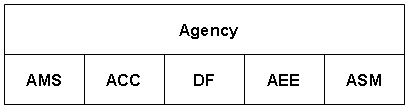
\includegraphics[scale=0.5]{figure/mobilec_lib_arch}
   \caption{Architecture of the Mobile-C library.}
   \label{fig:mobilec_lib_arch}
\end{center}
\end{figure*}
% FIGURE }}} 
%%%%%%%%%%%%%%%%%%%%%%%%%%%%%%%%%%%%%%%%%%%%%%%%%%%%%%%%%%%%%%%%%%%%%%

%%%%%%%%%%%%%%%%%%%%%%%%%%%%%%%%%%%%%%%%%%%%%%%%%%%%%%%%%%%%%%%%%%%%%%
% FIGURE {{{ 
\begin{figure*}[!t]
\begin{center}
   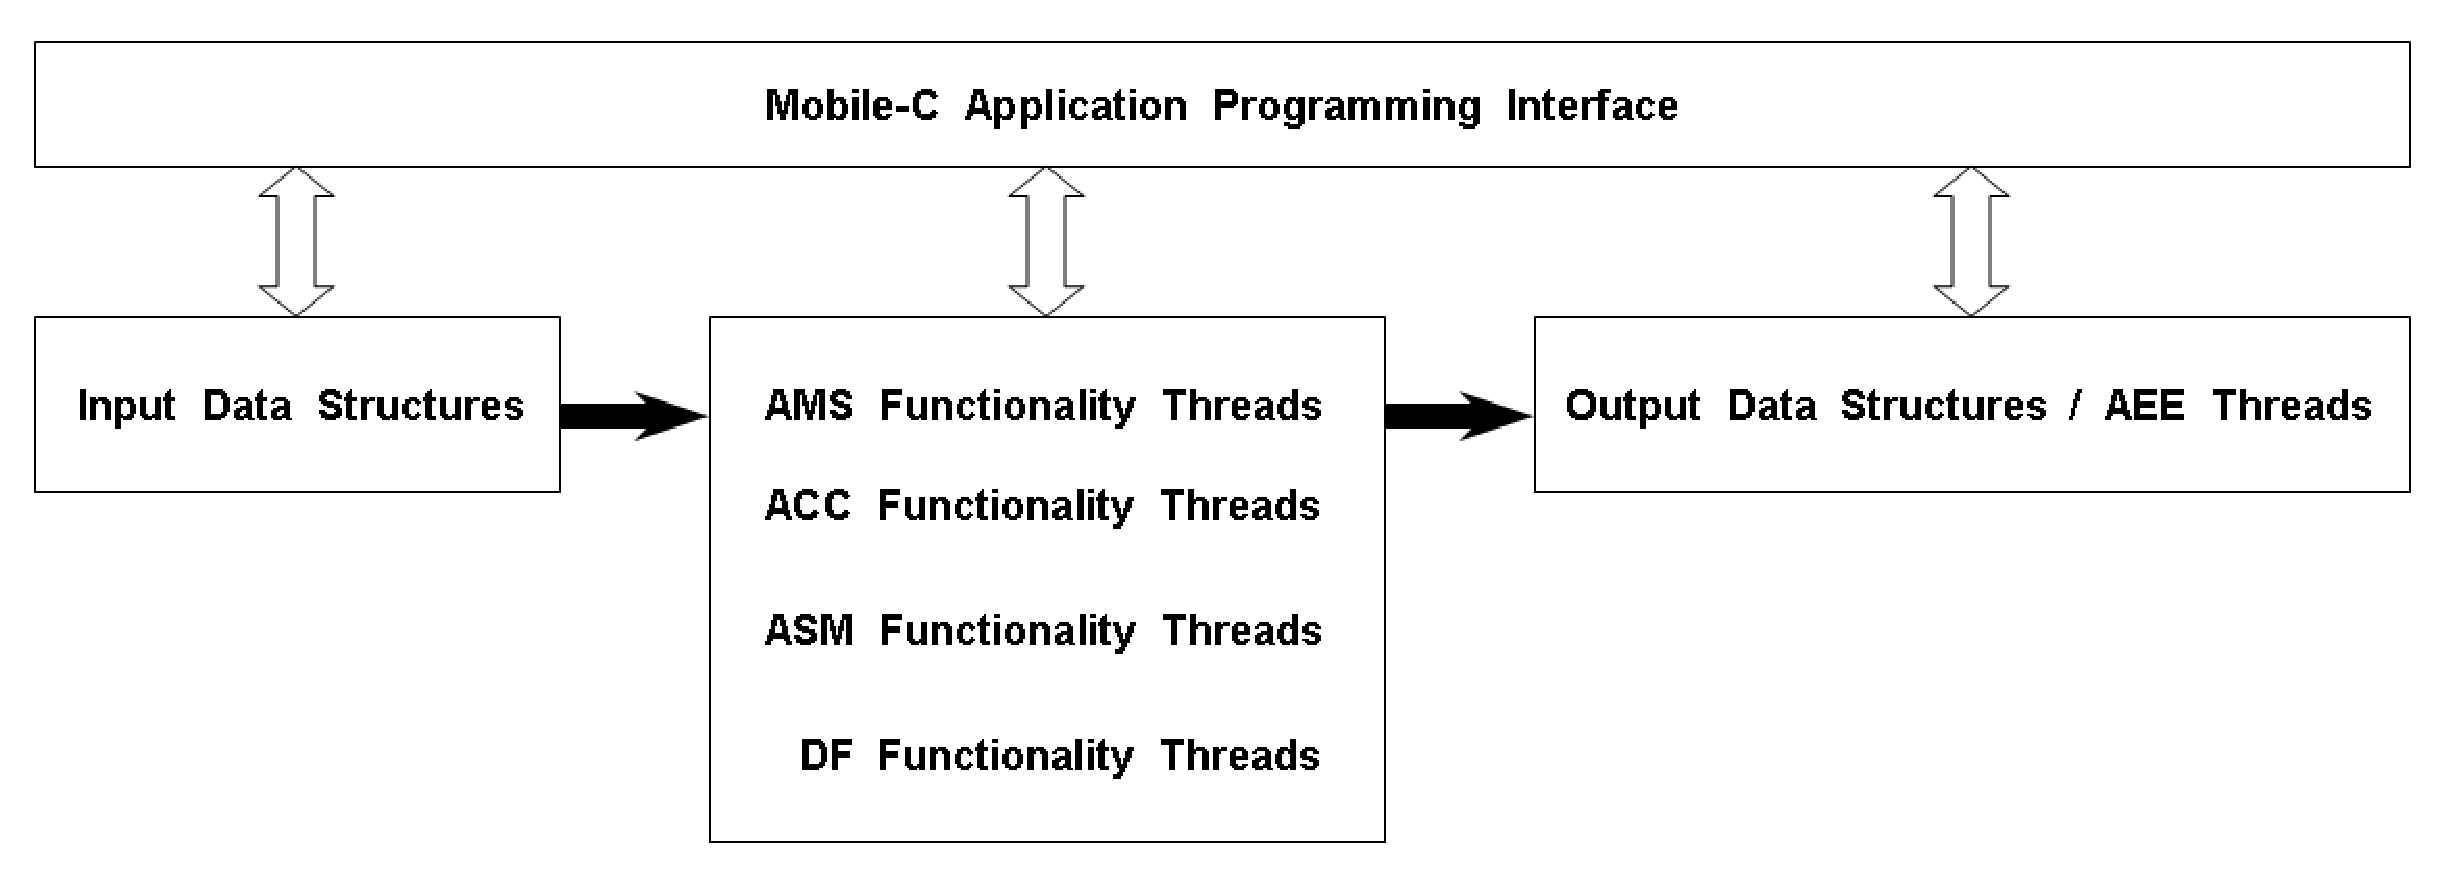
\includegraphics[scale=0.5]{figure/mobilec_lib_imp}
   \caption{Implementation overview of the Mobile-C library.}
   \label{fig:mobilec_lib_imp}
\end{center}
\end{figure*}
% FIGURE }}} 
%%%%%%%%%%%%%%%%%%%%%%%%%%%%%%%%%%%%%%%%%%%%%%%%%%%%%%%%%%%%%%%%%%%%%%

%%%%%%%%%%%%%%%%%%%%%%%%%%%%%%%%%%%%%%%%%%%%%%%%%%%%%%%%%%%%%%%%%%%%%%
% Architecture of the Mobile-C Library {{{
\subsection{Architecture of the Mobile-C Library \label{mobilec_arch}}
Figure \ref{fig:mobilec_lib_arch} illustrates the architecture of the 
Mobile-C library.
The Mobile-C library allows a Mobile-C agency to be embedded in a program to 
support C/C++ mobile agents.
A Mobile-C agency refers to a mobile agent platform within which mobile agents 
exist and operate.
The Mobile-C API gives users a full control over a Mobile-C agency and its 
different modules.
 
As a IEEE FIPA compliant mobile agent platform, a Mobile-C agency 
comprises three FIPA normative modules, Agent Management System (AMS), 
Agent Communication Channel (ACC) and Directory Facilitator (DF). 
Two additional modules, Agent Execution Engine (AEE) and 
Agent Security Manager (ASM), are included in a Mobile-C agency as well.
These modules provide different functionalities summarized as follows.

\textit{Agent Management System (AMS)}

\noindent
An AMS controls the creation, registration, execution, migration, 
persistence, and termination of a mobile agent. 
It maintains a directory of Agent Identifiers (AIDs) for registered mobile 
agents. 
Each mobile agent must register with an AMS in order to have a valid AID.

\textit{Agent Communication Channel (ACC)}

\noindent
An ACC routes messages between local and remote entities. 
It is responsible for the interactions between distributed components, such 
as inter-agent communication and inter-platform agent transport. 
The interactions can be performed through Agent Communication Language (ACL) 
message exchange.

\textit{Directory Facilitator (DF)}

\noindent
A DF serves yellow page services. 
Mobile agents wishing to advertise their services should register with a DF. 
Visiting mobile agents can search a DF for mobile agents providing the 
services they desire.

\textit{Agent Execution Engine (AEE)}

\noindent
An AEE serves as the execution environment for mobile agent code.
An AEE has to be platform independent in order to support the execution of 
mobile agents in a heterogeneous environment. 

Each AEE contains an Embedded Ch interpreter to interpret the agent C code.
By default, the agency will preload four interpreters upon startup for
interpreting agents. If more than four interpreters are required, the agency
will dynamically allocate extra interpreters as needed. See the reference for
\texttt{MC\_Initialize()} on page \pageref{api:MC_Initialize} for more info.

\textit{Agent Security Manager (ASM)}

\noindent
An ASM is responsible for maintaining securita policies for the host system.
Some sample tasks of an ASM include identifying users, protecting host 
resources, authenticating and authorizing mobile agents, and ensuring the 
security and integrity of mobile agents.
% }}} Architecture of the Mobile-C Library
%%%%%%%%%%%%%%%%%%%%%%%%%%%%%%%%%%%%%%%%%%%%%%%%%%%%%%%%%%%%%%%%%%%%%%

%%%%%%%%%%%%%%%%%%%%%%%%%%%%%%%%%%%%%%%%%%%%%%%%%%%%%%%%%%%%%%%%%%%%%%
% SUB: Implementation of the Mobile-C Library {{{
\subsection{Implementation of the Mobile-C Library}
Figure \ref{fig:mobilec_lib_imp} shows the implementation overview of the 
Mobile-C library.
The functionalities of each module of an agency are 
implemented as independent threads classified into five categories, that is, 
the AMS functionality threads, the ACC functionality threads, the DF 
functionality threads, the ASM functionality threads and the AEE threads.
Each AEE thread is launched by one of the AMS functionality threads.

The Mobile-C library provides API functions to specify which thread needs to 
be active or inactive when an agency is initialized.
It also provides API functions to access the input and output data structures 
associated with the functionality threads.
A Mobile-C agency maintains a list of synchronization variables that can be 
used with a group of Mobile-C functions to ensure synchronization among 
mobile agents and threads.
The sizes of the Mobile-C static and shared libraries for Linux are about 
500 KB and 390 KB, respectively.

The header file \textit{libmc.h} contains definitions of all the structures and 
functions of the Mobile-C library. 
Table \vref{mobilec_api_cbinary} lists the currently implemented functions 
for the binary space.

% }}} Implementation of the Mobile-C Library
%%%%%%%%%%%%%%%%%%%%%%%%%%%%%%%%%%%%%%%%%%%%%%%%%%%%%%%%%%%%%%%%%%%%%%

% }}} The Mobile-C Library
%%%%%%%%%%%%%%%%%%%%%%%%%%%%%%%%%%%%%%%%%%%%%%%%%%%%%%%%%%%%%%%%%%%%%%

% }}} Getting Started
%%%%%%%%%%%%%%%%%%%%%%%%%%%%%%%%%%%%%%%%%%%%%%%%%%%%%%%%%%%%%%%%%%%%%%

%%%%%%%%%%%%%%%%%%%%%%%%%%%%%%%%%%%%%%%%%%%%%%%%%%%%%%%%%%%%%%%%%%%%%%
% Composing Agents {{{
\chapter{Composing Agents}
Mobile-C agents are represented internally as XML data structures. However,
dealing with XML code requires background knowledge of XML and may be cumbersome.
To enhance the convenience of creating and deploying Mobile-C agents,
several different methods of creating agents from C source code files have
been implemented.

Agents may be composed from plain C source code. There are two main ways to
compose Mobile-C agents. Agents may be composed by using the
\texttt{compose\_send} commmand in the Mobile-C prompt, or by using the
\texttt{MC\_ComposeAgent*} series of API functions.

\section{Mobile-C Command Prompt \texttt{compose\_send} Command}
The \texttt{compose\_agent} takes a C source code file and creates
a fully functioning agent out of it. The \texttt{compose\_send} command
syntax is
\begin{verbatim}
compose_send <filename> <target host> <target port>
\end{verbatim}
Many details about an agent generated in this method, such as the agent's
name and owner, are dynamically generated when creating an agent using 
this method. 
\subsection{Example Execution Using the \texttt{compose\_send} Command}
The demo \texttt{prompt\_example} has been provided with the Mobile-C
package. Note that the source code for both servers is virtually identical to
that in Program \ref{prog:server.c}, except with added execution
instructions.
The demo program is initiated by starting the first agency, named
\texttt{server1}.
\begin{verbatim}
$ ./server1
Agency 1 started. Please start the second agency by running the command
"server2" on another terminal.

MobileC >
\end{verbatim}
Next, the second agency is started on a seperate terminal.
\begin{verbatim}
$ ./server2
Starting Agency...
You may now try the following commands:

  compose_send helloworld.c localhost 5050

The previous command will compose an agent using the source
code in "helloworld.c" and send it to the other agency at
port 5050. Then try this command:

  compose_send helloworld.c localhost 5051

This will send the "hello_world.c" agent to the local agency.
You may also try these commands at the other agency.

MobileC >
\end{verbatim}
Following the instructions on the second agency, we execute the 
suggested \texttt{compose\_send} command. The first agency terminal
now appears as such:
\begin{verbatim}
$ ./server1
Agency 1 started. Please start the second agency by running the command
  "server2" on another terminal.

MobileC > Hello, world!
\end{verbatim}
Note that the source file \texttt{helloworld.c} has been composed into a 
mobile agent, migrated to the \texttt{server1} agency, and executed.

\section{Mobile-C \texttt{MC\_ComposeAgent*} Functions}
There also exist a set of API functions which compose agents from C source
files. These functions are
\begin{itemize}
\item \texttt{MC\_ComposeAgent()} : Compose an agent from program source code. 
\item \texttt{MC\_ComposeAgentWithWorkgroup()} : Compose an agent from program source code with a workgroup code. 
\item \texttt{MC\_ComposeAgentFromFile()} : Compose an agent from a program source code file. 
\item \texttt{MC\_ComposeAgentFromFileWithWorkgroup()} : Compose an agent from a program source code file with a workgroup code. 
\item \texttt{MC\_AgentAddTask()} : Add an additional task to an already formed agent.
\item \texttt{MC\_AgentAddTaskFromFile()} : Add an additional task to an already formed agent from a C source code file.
\end{itemize}
For an example of the usage of these functions, please refer to program
\ref{prog:compose_multi_task_agent}.

\begin{Program}[p]
\begin{center}
   {\footnotesize \linespread{1.0}
     \verbatiminput{../demos/composing_agents/multi_task_example/client_abridged.c}}
\end{center}
\caption{An agency building an agent with multiple tasks from seperate source code files.}
\label{prog:compose_multi_task_agent}
\end{Program}

\section{Agent Workgroups}
In order to provide an added layer of organization and security, agents
may be created which belong to a workgroup. A workgroup's name may be an
ASCII text string of any length. If an agent belongs in a workgroup,
then certain actions on that agent may only be performed by other agents
in the same workgroup. Thus, if a group of agents keeps their workgroup
name private, no agents outside of that group will be able to terminate,
delete, or otherwise affect the agents within the workgroup. All agents are
still able to interact through FIPA ACL messages.

For an example of agent workgroups in action, please see the demo program
in the\\
 \texttt{demos/agent\_workgroup\_example} directory. 
% }}}
%%%%%%%%%%%%%%%%%%%%%%%%%%%%%%%%%%%%%%%%%%%%%%%%%%%%%%%%%%%%%%%%%%%%%%


%%%%%%%%%%%%%%%%%%%%%%%%%%%%%%%%%%%%%%%%%%%%%%%%%%%%%%%%%%%%%%%%%%%%%%
% Agent Data {{{
\chapter{Agent Data}
Agents have the ability to carry pieces of data with them as they migrate from
host to host. The data carried by an agent can be categorized into two broad
types: ``agent return data'' and ``agent saved variables''. 

\section{Agent Return Data}
  ``Agent return data'' is typically used to store a piece of data being
returned to the agent's home agency. For instance, if an agent is given a task
to obtain a single result from a remote host, the agent might store the result
as its agent return data. An agent may hold a single return value for each one
of its tasks. The return value may be of any standard C type, or an array of 
such a type. For instance, the \texttt{double} type, as well as
\texttt{double[5][3]} are both valid types for a piece of agent return data,
since both are examples of a standard C type or an array of a standard type.
User defined structs and unions may not be returned as a piece of return data.
 
In order to return a variable as agent return data, the name of the return variable
simply needs to be specified when composing the agent. No further API calls need to be
executed from within the agent code. Note that the return variable must be declared as
a global variable in the agent code.
For an example of an agent with multiple tasks returning information to its home agency,
please see Program \ref{prog:compose_multi_task_agent} on page
\pageref{prog:compose_multi_task_agent}.

\section{Agent Saved Variables} 
An ``agent saved variable'' is also carried with an agent as it migrates. However,
this type of variable is typically used for data that the agent itself has access
to as it completes its tasks. Furthermore, an agent may save the value of as many
variables as it desires per task. For instance, during an agent's first task, it
may save various values, like the number of other agents on the agency as an
\texttt{int}, and the name of the agency as a \texttt{char[80]}. After it
migrates to it's second task, it may access the variables it saved previously
on the first host. In this way, an agent could calculate the total number of
active agents in an agency network. In summary,

\begin{tabular}{l|cc}
 & Agent Return Data & Agent Saved Variable \\
\hline
May save multiple variables per task & & X \\
\hline
Data easily retrieved by home agency & X & X \\
\hline
Data saved to agent automatically  & & \\
without agent-space API calls & X & \\
\hline
Agent can access its own saved data & & X
\end{tabular}

\vspace{0.18in}
For example, consider an agent with the following tasks. The agent's first task
appears as such:
\verbatiminput{../demos/agent_migration_message_format/agent_saved_variables_example/task1.c}
Note that the variable to be saved must be a global variable. In the agent code, the agent
performs a call to the function \texttt{mc\_AgentVariableSave(mc\_current\_agent, "savevar");}
The first argument in the function is a handle to an agent. The handle \texttt{mc\_current\_agent} is
a special handle an agent has to itself. The second argument is a character string denoting the
name of the variable to save. In effect, this code saves the value of \texttt{savevar} to
itself. As shown in the preceding code, the \texttt{mc\_AgentVariableSave()} function may
be called multiple times on differing variable types and arrays. Each variable will be
saved to the agent prior to migration.

Here is an example of the agent's second task's code:
\verbatiminput{../demos/agent_migration_message_format/agent_saved_variables_example/task2.c}
Note the call to \texttt{mc\_AgentVariableRetrieve(mc\_current\_agent,
"savevar", 0);} in this code example. This function attempts to retrieve a
pointer to the saved variable. The first argument, as seen before, is a handle
to the agent itself. The second variable is the name of the variable to
retrieve. The third argument is the task from which to retrieve the variable,
with the value \texttt{0} being the first task. If the call succeeds, it will
return a valid pointer to the saved variable. If it fails, the function returns
\texttt{NULL}.



% Chapter: Agent Data }}}
%%%%%%%%%%%%%%%%%%%%%%%%%%%%%%%%%%%%%%%%%%%%%%%%%%%%%%%%%%%%%%%%%%%%%%


%%%%%%%%%%%%%%%%%%%%%%%%%%%%%%%%%%%%%%%%%%%%%%%%%%%%%%%%%%%%%%%%%%%%%%
% Mobile-C Agent Migration Message Format {{{
\chapter{Mobile-C Agent Migration Message Format}
\section{General Message Format \label{sec:gen_message_format}}
\begin{Program}
\begin{center}
   {\scriptsize \linespread{1.0} \verbatiminput{../demos/getting_started/hello_world/test1.xml}}
\end{center}
\caption{A rudimentary agent. (demos/getting\_started/hello\_world/test1.xml)}
\label{prog:hello_agent}
\end{Program}
The message format for an agent migration message is designed such that
multiple tasks and multiple code blocks can be migrated from agency to
agency. The message is an XML message with encapsulated C code. An example
of a rudimentary agent can be seen in Program \ref{prog:hello_agent} on 
page \pageref{prog:hello_agent}. 
Following is a brief description of each XML tag.
\begin{itemize}
\item \texttt{MESSAGE}: This tag indicates to Mobile-C that the following data
  is a Mobile-C message. The message type is included in the attribute
  ``message''.
\item \texttt{MOBILE\_AGENT}: This tag indicates that the contained data is a 
  Mobile-C agent.
\item \texttt{AGENT\_DATA}: This tag indicates that the contained data is data pertaining
  to this particular agent.
\item \texttt{NAME}: The name of the agent.
\item \texttt{OWNER}: The owner of the agent. 
\item \texttt{HOME}: The home of the agent. Any agent that has data to ``return'' will
	return it to this address by default.
\item \texttt{WG\_CODE}: The workgroup code of the agent. Workgroup codes are
kept secret by the agent. Only agents with matching workgroup codes are allowed
to perform certain operations on each other, such as agent deletion.
\item \texttt{TASKS}: This indicates that the following information pertains to the
  task or tasks the agent is intended to perform. Attributes found under the
  \texttt{TASKS} tag include:
  \begin{itemize}
    \item \texttt{task} : The total number of tasks the agent has.
    \item \texttt{num} : The task that the agent is currently on.
  \end{itemize}
\item \texttt{TASK}: Each seperate \texttt{TASK} tag indicates a seperate task for the agent
  to perform. The tasks may be seperate hosts and/or code blocks. In the
  rudimentary example, there is only one task. Listed below are the attributes of 
  \texttt{TASK} tags.
  \begin{itemize}
  \item \texttt{num}:           The number of the task. The first task is task number zero.
  \item \texttt{complete}:      Completeness of the task
  \item \texttt{server}:        The host to perform the task
  \item \texttt{return}:        Name of the return variable
  \item \texttt{persistent}:    Persistence of the agent
  \item \texttt{return\_value}: Return value, if not an array
  \item \texttt{code\_id}:      ID of the code block to execute
  \end{itemize}
\textit{complete} and \textit{server} are mandatory attributes, and others are 
optional attributes.  
\item AGENT\_CODE: Each AGENT\_CODE block represents a block of code that 
  the agent may execute. Agents with multiple code blocks may decide at run-time
  which block to execute. Valid attributes under the \texttt{AGENT\_CODE} tag
  include
  \begin{itemize}
    \item \texttt{id}: The id of the code segment, as referenced by the \texttt{TASK} 
      attribute, \texttt{code\_id}.
  \end{itemize}
\end{itemize}

\section{Multiple Tasks with a Single Code Block}
An agent may have an indefinite number of tasks. The agent will perform the tasks
in ther order that they are stated in the XML file, completing each one before
continuing to the next host. Following is an example of an agent which has
multiple tasks to perform, executing the same code block at each new host.
See Program \ref{prog:single_code_block} on page \pageref{prog:single_code_block} 
for an example.
\begin{Program}[p]
\begin{center}
   {\footnotesize \linespread{1.0} 
     \verbatiminput{../demos/composing_agents/multi_task_example/test_single_code_block1.xml}}
\end{center}
\caption{An example agent containing two tasks and a single code block.
  Note that variables ``mc\_host\_name'' and ``mc\_task\_progress'' are special built-in variables described in Table \vref{tab:agent_space_variables}.
  \index{mc\_host\_name}
  \index{mc\_task\_progress}
  \texttt{(<MCPACKAGE>/demos/composing\_agents/multi\_task\_example/test\_single\_code\_block.xml)} }
\label{prog:single_code_block}
\end{Program}
\addtocounter{Program}{-1}
\begin{Program}[p]
\begin{center}
   {\footnotesize \linespread{1.0} 
     \verbatiminput{../demos/composing_agents/multi_task_example/test_single_code_block2.xml}}
\end{center}
\caption{(Continued)}
\end{Program}

\section{Multiple Tasks with Multiple Code Blocks}
See Program \ref{prog:multi_code_block} on page \pageref{prog:multi_code_block}
for a more complicated example of agent code including multiple tasks and
  multiple code blocks. Note that each code block has an associated ID which is 
  refered to in the respective ``DATA'' tags. Also note that more than one ``DATA'' tag
  may refer to the same code block. Thus, an agent may have more ``DATA'' tags than
  code blocks.

\begin{Program}[p]
\begin{center}
   {\footnotesize \linespread{1.0} 
     \verbatiminput{../demos/composing_agents/multi_task_example/test_multi_code_block1.xml}}
\end{center}
\caption{An example agent containing two tasks and two code blocks. 
  \texttt{(<MCPACKAGE>/demos/composing\_agents/multi\_task\_example/test\_multi\_code\_block.xml)}} 
\label{prog:multi_code_block}
\end{Program}
\addtocounter{Program}{-1}
\begin{Program}[p]
\begin{center}
   {\footnotesize \linespread{1.0} 
     \verbatiminput{../demos/composing_agents/multi_task_example/test_multi_code_block2.xml}}
\end{center}
\caption{ (Continued) }
\end{Program}

\section {Multiple Mobile Agent performs Task on Multiple Hosts}
Program \ref{prog:multi_mobile_agent_client} on page \pageref{prog:multi_mobile_agent_client} is a client that sends two different mobile agents to two different hosts. In for loop, it waits for the arrival signal of mobile agent. When an agent arrives it prints the result and delete that agent. For loop is iterated same as total number of mobile agents send by client. The two mobile agents having different name are shown in Program \ref{prog:mobile_agent_1} and Program \ref{prog:mobile_agent_2}:  

\begin{Program}[p]
\begin{center}
   {\footnotesize \linespread{1.0}
     \verbatiminput{../demos/agent_migration_message_format/multi_data_retrieval/client.c}}
\end{center}
\caption{A client program that sends two mobile agents to two different hosts
  \texttt{(<MCPACKAGE>/demos/agent\_migration\_message\_format/multi\_data\_retrieval/client.c)}}
\label{prog:multi_mobile_agent_client}
\end{Program}

\begin{Program}[p]
\begin{center}
   {\footnotesize \linespread{1.0}
     \verbatiminput{../demos/agent_migration_message_format/multi_data_retrieval/test1.xml}}
\end{center}\caption{First mobile agent name "mobagent1" send by client (Program 6) to server 1   
  \texttt{(<MCPACKAGE>/demos/agent\_migration\_message\_format/multi\_data\_retrieval/test1.xml)}}
\label{prog:mobile_agent_1}
\end{Program}

\begin{Program}[p]
\begin{center}
   {\footnotesize \linespread{1.0}
     \verbatiminput{../demos/agent_migration_message_format/multi_data_retrieval/test2.xml}}
\end{center}\caption{Second mobile agent name "mobagent1" send by client (Program 6) to server 2
  \texttt{(<MCPACKAGE>/demos/agent\_migration\_message\_format/multi\_data\_retrieval/test2.xml)}}
\label{prog:mobile_agent_2}
\end{Program}

\section{Agent Return Messages}
If the ``\texttt{name}'' attribute in an agent's ``\texttt{DATA}'' tag
is not set to ``\texttt{no-return}'', the agent will generate an
agent-return message upon completion of all of its tasks. The agent will
generate a return message containing the contents of the variable name
specified in the ``\texttt{name}'' attribute. For instance, Program
\vref{prog:agent_with_return_data} shows a simple agent which 
will migrate to another agency, generate a three-dimensional array called
``\texttt{a}'', and return the contents of the array to the ``\texttt{HOME}''
host upon completion. Note that the return variable must be global
so that the contents are not destroyed upon completion of the \texttt{main}
function. 
  
  An example of the return message that is generated by
this agent can be seen in Program \vref{prog:return_agent}. Notice also in
the return message that the variable type has been changed from ``int'' as it
was in the original program to ``short'' and that the ``\texttt{dim}'' attribute
has been changed to $3$. This is because Mobile-C automatically
checks the type and dimension of the variable it is returning and assign
those attributes automatically.

\begin{Program}[p]
\begin{center}
   {\footnotesize \linespread{1.0} 
     \verbatiminput{../demos/agent_migration_message_format/mc_array_return_example/agent.xml}}
\end{center}
\caption{An agent which returns data upon completion of it's tasks.}
\label{prog:agent_with_return_data}
\end{Program}

\begin{Program}[p]
\begin{center}
   {\footnotesize \linespread{1.0} 
     \verbatiminput{../demos/agent_migration_message_format/mc_array_return_example/return_agent.xml}}
\end{center}
\caption{Agent return data xml format. Note: This XML code has been reformatted
  to a more human-readable format. The actual format generated may differ.}
\label{prog:return_agent}
\end{Program}

\section{Agent Saved Variables}
As of Mobile-C version 1.10.0, Mobile-C agents have the ability to save an 
arbitrary number of variables while migrating from task to task. Agents may
use the agent-space api functions \texttt{mc\_AgentVariableSave()} and
\texttt{mc\_AgentVariableRetrieve} to save and later retrieve variables.
An example agent which does this may be viewed at the documentation for
the \texttt{mc\_AgentVariableSave()} and \linebreak \texttt{mc\_AgentVariableRetrieve()}
functions on pages \pageref{apidoc:mc_AgentVariableSave} and 
\pageref{apidoc:mc_AgentVariableRetrieve}, respectively.

As the agent is migrating from host to host with saved data, the data is 
encapsulated in the agent's XML code. \texttt{<DATA>} tags are created as
children of each \texttt{<TASK>} tag to store data. See Program 
\ref{prog:migrating_agent} for an example of an agent that is migrating
with saved data. The valid attributes within a \texttt{<DATA>} tag are
\begin{itemize}
\item \texttt{name}: The name of the saved variable.
\item \texttt{dim}: The array dimension of the saved variable. 
\item \texttt{type}: The type of the variable.
\item \texttt{value}: (optional) If the variable has zero dimensions, the
  value is stored in this attribute. Otherwise, children \texttt{<ROW>} 
  tags must be created to store the array.
\end{itemize}

Each \texttt{<DATA>} tag may also have children \texttt{<ROW>} tags, if
the data is an array. The valid attributes of the \texttt{<ROW>} tags are
\begin{itemize}
\item \texttt{index}: The index of the row.
\end{itemize}
Note also that each \texttt{<ROW>} tag may contain additional \texttt{<ROW>}
children depending on the dimension of the array being stored.

The Mobile-C XML Data Type Definition (DTD), which defines the format of a
well-formed Mobile-C agent migration message, may be seen in Section
\ref{sec:xml_dtd} on page \pageref{sec:xml_dtd}.

\section{Stationary/Persistent Mobile Agents}
A Stationary agent may be achieved in Mobile-C simply by creating an agent which
never migrates. This is commonly achieved using a couple of different
techniques.
\subsection{An Agent with an Infinite Task}
An agent may be considered stationary if it's task never ends. For instance, if
the task of an agent is of the form:
\begin{verbatim}
while(1)
{
    cmd = wait_for_command();
    execute_command(cmd);
}
\end{verbatim}
Since the previous task never ends, the agent will never terminate and the agent
will remain stationary in it's agency. 

\subsection{The ``\texttt{persistent}'' Agent Flag}
The ``\texttt{persistent}'' flag as mentioned in Section
\ref{sec:gen_message_format} may be used to create a persistent agent. The
example described in Chapter \ref{chap:interface_binary_to_agent} uses such a
technique. This technique creates an agent which is not automatically flushed by the agency
after it completes it's task. Thus, the agent remains dormant and stationary in
the agency without external stimulus.

\subsubsection{Terminating Persistent Agents}
Persistent agents should be terminated when they are no longer needed to free
up resources. They may be terminated by using the API functions 
\texttt{MC\_DeleteAgent()} or \texttt{MC\_TerminateAgent()} functions from C-space,
or the functions \texttt{mc\_DeleteAgent()} or \texttt{MC\_TerminateAgent()} functions 
from agent-space. Since a persistent agent cannot terminate itself, it is up to either
the host agency or another agent to terminate the persistent agent.

\begin{Program}[ph]
\begin{center}
{\footnotesize \linespread{1.0}
\verbatiminput{../demos/agent_migration_message_format/agent_saved_variables_example/migrating_agent.xml.part1}}
\end{center}
\caption{\label{prog:migrating_agent} This XML format illustrates an agent which is currently
in the process of migrating with saved data. Note that the agent contains two tasks, and the
first task has been completed. This file is a snapshot of the agent as it is in transit from
task '0' to task '1'. Note the \texttt{<DATA>} tags which store the three variables
referenced by the \texttt{mc\_AgentSaveVariable()} function from within the code, storing
two integers and an integer array. Note that in general, any data type may be stored, including
multi-dimensional arrays.}
\end{Program}
\addtocounter{Program}{-1}
\begin{Program}[ph]
\begin{center}
{\footnotesize \linespread{1.0}
\verbatiminput{../demos/agent_migration_message_format/agent_saved_variables_example/migrating_agent.xml.part2}}
\end{center}
\caption{(Continued)}
\end{Program}


% }}} Mobile-C Agent Migration Message Format
%%%%%%%%%%%%%%%%%%%%%%%%%%%%%%%%%%%%%%%%%%%%%%%%%%%%%%%%%%%%%%%%%%%%%%

%%%%%%%%%%%%%%%%%%%%%%%%%%%%%%%%%%%%%%%%%%%%%%%%%%%%%%%%%%%%%%%%%%%%%%
% {{{ Mobile-C FIPA Compliant ACL Messages
\chapter{Mobile-C FIPA Compliant ACL Messages \label{chap:fipa}}
Mobile-C has the ability to send and receive FIPA compliant
agent communication language (ACL) messages. More information
about FIPA, the Foundation for Intellegent Physical Agents, may be
found at \texttt{http://www.fipa.org}. This functionality allows
Mobile-C agent to communicate with each other, as well as with 
agents from other agencies that are also FIPA compliant. Demos
of communication with JADE agents may be found in the directories
\texttt{<MCPACKAGE>/demos/jade\_to\_mc\_example} and \\
\texttt{<MCPACKAGE>/demos/mc\_to\_jade\_example}.

%{{{ Constructing and Sending an ACL Message
\section{Constructing and Sending an ACL Message}
The general process for constructing an ACL message involves
filling out required portions of an ACL message structure of type
\texttt{struct fipa\_acl\_message\_s} and passing the message to the
\texttt{MC\_AclSend()} function. A number of helper functions 
exist in order to simplify the process of allocating memory and setting
certain fields of the acl message. 
Some typical functions used to compose a new ACL message are the following:
\begin{itemize}
\item \texttt{MC\_AclSetPerformative}: Set the FIPA performative of the message. See Program
  \ref{prog:fipa_enum} for a complete listing of valid FIPA performative enumerations.
\item \texttt{MC\_AclSetSender}: Sets the 'sender' field of the message.
\item \texttt{MC\_AclAddReceiver}: Adds addresses to the 'receiver' field of the message.
\item \texttt{MC\_AclSetContent}: Sets the 'content' field of an ACL message.
\end{itemize}
A detailed example of sending and receiving messages will be presented in
Chapter \ref{chap:stationary_agent}.
%}}}

%{{{Receiving an ACL Message 
\section{Receiving an ACL Message}
Every agent residing on a Mobile-C agency has a mailbox allocated to it.
At any time, the agent may check the mailbox for new ACL messages, or an
agent may choose to wait on an empty mailbox until a new message arrives.
These two tasks are done by the functions \texttt{MC\_AclRetreive()} and
\texttt{MC\_AclWaitRetrieve()}, respectively. 
Another useful function which may be used with a received ACL message is the
\texttt{MC\_AclReply()} function. This function takes an ACL message as an
input argument and automatically forms an ACL reply message addressed to the
original sender. Note that the performative and new sender fields in the reply
message are not automatically initialized and will still need to be set by
the agent. A detailed example of an agent receiving and replying to a message
may be found in Chapter \ref{chap:stationary_agent}.

\begin{Program}[!t]
\begin{center}
   {\footnotesize \linespread{1.0} 
\begin{verbatim}
enum fipa_performative_e
{
  FIPA_ERROR=-1,
  FIPA_ZERO,
  FIPA_ACCEPT_PROPOSAL,
  FIPA_AGREE,
  FIPA_CANCEL,
  FIPA_CALL_FOR_PROPOSAL,
  FIPA_CONFIRM,
  FIPA_DISCONFIRM,
  FIPA_FAILURE,
  FIPA_INFORM,
  FIPA_INFORM_IF,
  FIPA_INFORM_REF,
  FIPA_NOT_UNDERSTOOD,
  FIPA_PROPOGATE,
  FIPA_PROPOSE,
  FIPA_PROXY,
  FIPA_QUERY_IF,
  FIPA_QUERY_REF,
  FIPA_REFUSE,
  FIPA_REJECT_PROPOSAL,
  FIPA_REQUEST,
  FIPA_REQUEST_WHEN,
  FIPA_REQUEST_WHENEVER,
  FIPA_SUBSCRIBE
};
\end{verbatim}
   }
\end{center}
\caption{Fipa Performative Enumerations.}
\label{prog:fipa_enum}
\end{Program}

\pagebreak
\clearpage
\pagebreak
%}}} Section: Receiving an ACL Message

%}}} Chapter: Mobile-C FIPA Compliant ACL Messages
%%%%%%%%%%%%%%%%%%%%%%%%%%%%%%%%%%%%%%%%%%%%%%%%%%%%%%%%%%%%%%%%%%%%%%

%%%%%%%%%%%%%%%%%%%%%%%%%%%%%%%%%%%%%%%%%%%%%%%%%%%%%%%%%%%%%%%%%%%%%%
% Mobile-C Binary Stationary Agents {{{
\chapter{Mobile-C Binary Stationary Agents \label{chap:stationary_agent}}
Mobilec has support for hosting binary-space stationary agents. The
agents are implemented as system threads. As such, the only limit 
to the number of stationary agents residing on an agency are the
system resources of the host agency. 

The binary agents are able to call any of the C-space API functions, such as
\texttt{MC\_AclWaitRetrieve()}. This allows stationary agents to communicate
and interact with other mobile and stationary agents using FIPA ACL messages,
as introduced in Chapter \ref{chap:fipa}.

Stationary agents may be used in any application in which agent mobility is
unnecessary. Stationary agents can typically perform any task a mobile agent
can perform, except migration. Furthermore, stationary agents tend to execute
faster and consume less system resources.

Mobile-C stationary agent threads are added using the
\texttt{MC\_AddStationaryAgent()} API function. See Program 
\ref{prog:stationary_agent_server} for an example of a stationary agent. 

\begin{Program}[!t]
\begin{center}
   {\footnotesize \linespread{1.0} \verbatiminput{../demos/binary_stationary_agents/stationary_agent_communication/server.c}}
\end{center}
\caption{A sample program which starts a single stationary agent that responds to FIPA ACL messages.}
\label{prog:stationary_agent_server}
\end{Program}

The \texttt{MC\_AddStationaryAgent()} function takes three arguments:
\begin{enumerate}
\item A handle to the home agency. This is the agency the new agent will reside under.
\item The agent thread. This is a pointer to a function which will execute and act as
the stationary agent. If the function returns, the stationary agent is terminated.
\item An optional argument to pass to the agent. If additional information or data needs
to be passed to the stationary agent thread, a pointer of any type may be supplied as the
third argument to \\
\texttt{MC\_AddStationaryAgent()}. This pointer may later be retrieved
with the \\
\texttt{MC\_AgentInfo\_GetAgentArgs()} function from within the agent.
\end{enumerate}

The stationary agent thread must have a prototype of the form
\begin{verbatim}
void* agent_func_name(stationary_agent_info_t* agent_info);
\end{verbatim}
As seen in the prototype, the agent thread receives an argument of type
\texttt{stationary\_agent\_info\_t}. This special type is a structure 
which contains information about the the agent, such as its name, and the
location of its mailbox. Certain information may be retrieved from the 
function parameter by using the \texttt{MC\_AgentInfo\_*} series of API
functions, which include:
\begin{itemize}
\item \texttt{MC\_AgentInfo\_GetAgency()} : Retrieves a handle to the host agency.
\item \texttt{MC\_AgentInfo\_GetAgent()} : Retrieves a handle to the agent
information structure.
\item \texttt{MC\_AgentInfo\_GetAgentArgs()} : Retrieves the pointer that was
given as an agent argument during the call to \texttt{MC\_AddStationaryAgent}.
\end{itemize}

Example usage of these functions may be seen in Program \ref{prog:stationary_agent_server}.
%}}}
%%%%%%%%%%%%%%%%%%%%%%%%%%%%%%%%%%%%%%%%%%%%%%%%%%%%%%%%%%%%%%%%%%%%%%

%%%%%%%%%%%%%%%%%%%%%%%%%%%%%%%%%%%%%%%%%%%%%%%%%%%%%%%%%%%%%%%%%%%%%%
% Interface between Binary and Mobile Agent Spaces {{{
\chapter{Interface between Binary and Mobile Agent Spaces
\label{chap:interface_binary_to_agent}}
An embeddable C/C++ interpreter Ch was chosen to be the AEE in the Mobile-C 
library to support C/C++ mobile agents. 
Therefore, in order to access the variables, functions, and data sets in 
the mobile agent space from the binary space, Ch must be first embedded in the 
binary space.
The function \textit{MC\_GetAgentExecEngine()} \index{MC\_GetAgentExecEngine()} in 
Table \ref{mobilec_api_cbinary} returns the AEE associated with a mobile agent 
to the binary space.
Using the AEE returned by \textit{MC\_GetAgentExecEngine()}, all of the 
Embedded Ch functions~\cite{EmbeddedCh} can be called in a binary C/C++ 
program to access the variables, functions, and data sets defined in the 
mobile agent space.
The Embedded Ch toolkit also allows mobile agent code to invoke C/C++ 
functions defined in a binary C/C++ program.

The Embedded Ch toolkit reduces the complexity of heterogeneous development 
environment for both embedded scripting and applications. 
With the consistent C/C++ code base, it can significantly reduce the effort 
in the software development and maintenance. 
Moreover, with the Embedded Ch toolkit, C/C++ applications can be extended 
with all the features of Ch including built-in string type for scripting. 
The Embedded Ch toolkit has a small footprint. 
The pointer and time deterministic nature of the C language provide a 
perfect interface with hardware in real-time systems.

\section{Using an Agent Initialization Callback Function to Intergrate Binary
and Script Space Code}
The user may register a callback function to be called during the initialization
of mobile agents inside of an agency. This allows the user to fine-tune 
an agent and the Ch interpreter before an agent is executed. The callback
function is added using the \texttt{MC\_AddAgentInitCallback()} function,
and the callback function is of the form
\begin{verbatim}
int callback(ChInterp_t interp, MCAgent_t agent, void* user_data);
\end{verbatim}
The user may call any applicable Ch API function on the interpreter,
as well as any applicable Mobile-C API function on the supplied agent.
For instance, the user may use the \texttt{Ch\_DeclareVar()} function
to declare extra variables inside of the interpereter which the agent
will be able to access during its execution. 

The demo located at \texttt{demos/cspace-agentspace\_interface/agent\_init\_callback/} 
provides a demonstration of the callback function. This demo uses the callback
function to declare a new function in each of the incoming agent interpreters
called \texttt{mult()}, which simply multiplies two numbers together. This
means that any incoming agent will be able to call the \texttt{mult()} function,
which resides in C-space, from the agent script-space. This demo may also be seen with
the documentation for \texttt{MC\_AddAgentInitCallback()} on page \pageref{api:MC_AddAgentInitCallback()}.

%%%%%%%%%%%%%%%%%%%%%%%%%%%%%%%%%%%%%%%%%%%%%%%%%%%%%%%%%%%%%%%%%%%%%%
% Invoke a Mobile Agent Space Function from Binary Space {{{
\noindent
\section{Invoke a Mobile Agent Space Function from Binary Space}
%%%%%%%%%%%%%%%%%%%%%%%%%%%%%%%%%%%%%%%%%%%%%%%%%%%%%%%%%%%%%%%%%%%%%%
% client.c {{{
\begin{Program}[!t]
\begin{center}
   {\footnotesize \linespread{1.0} 
     \verbatiminput{../demos/cspace-agentspace_interface/persistent_example/client.c}}
\end{center}
\caption{ A program which sends a persistent mobile agent.
  \texttt{(<MCPACKAGE>/demos/cspace-agentspace\_interface/persistent\_example/client.c)}}
\label{prog:client_ex2.c}
\end{Program}
% }}} client.c
%%%%%%%%%%%%%%%%%%%%%%%%%%%%%%%%%%%%%%%%%%%%%%%%%%%%%%%%%%%%%%%%%%%%%%
%%%%%%%%%%%%%%%%%%%%%%%%%%%%%%%%%%%%%%%%%%%%%%%%%%%%%%%%%%%%%%%%%%%%%%
% test1.xml {{{
\begin{Program}[!t]
\begin{center}
   {\footnotesize \linespread{1.0} 
     \verbatiminput{../demos/cspace-agentspace_interface/persistent_example/test1.xml}}
\end{center}
\caption{A persistent mobile agent. Agents marked ``persistent'' are
  not flushed from the agency after they terminate.
    \texttt{(<MCPACKAGE>/demos/cspace-agentspace\_interface/persistent\_example/test1.xml)}}
\label{prog:mobileagent_ex2.xml}
\end{Program}
% }}} test2.xml
%%%%%%%%%%%%%%%%%%%%%%%%%%%%%%%%%%%%%%%%%%%%%%%%%%%%%%%%%%%%%%%%%%%%%%
%%%%%%%%%%%%%%%%%%%%%%%%%%%%%%%%%%%%%%%%%%%%%%%%%%%%%%%%%%%%%%%%%%%%%%
% host.c {{{
\begin{Program}[!t]
\begin{center}
   {\footnotesize \linespread{1.0} 
     \verbatiminput{../demos/cspace-agentspace_interface/persistent_example/server.c}}
\end{center}
\caption{A Mobile-C agency.
 \texttt{(<MCPACKAGE>/demos/cspace-agentspace\_interface/ persistent\_example/server.c)}}
\label{prog:server_ex2.c}
\end{Program}
% }}} host.c
%%%%%%%%%%%%%%%%%%%%%%%%%%%%%%%%%%%%%%%%%%%%%%%%%%%%%%%%%%%%%%%%%%%%%%
%%%%%%%%%%%%%%%%%%%%%%%%%%%%%%%%%%%%%%%%%%%%%%%%%%%%%%%%%%%%%%%%%%%%%%
% FIGURE {{{
\begin{figure*}[!t]
\begin{center}
   {\footnotesize \linespread{1.0} \verbatiminput{../demos/cspace-agentspace_interface/persistent_example/server_output.txt}}
   \caption{Output from the binary server program.}
   \label{fig:example2_output}
\end{center}
\end{figure*}
% FIGURE }}}
%%%%%%%%%%%%%%%%%%%%%%%%%%%%%%%%%%%%%%%%%%%%%%%%%%%%%%%%%%%%%%%%%%%%%%

This example illustrates how to call a function defined in mobile agent 
code by using the Mobile-C library and Embedded Ch toolkit. 
The mobile agent in this example is a persistent agent, which is not removed 
upon termination of its execution.

The client program shown in Program \vref{prog:client_ex2.c} starts a Mobile-C 
agency listening on port \textit{5050} by the function 
\textit{MC\_Initialize()}, and sends a mobile agent to the remote agency 
running on host \textit{localhost} at port \textit{5051} through 
the function \textit{MC\_SendAgentMigrationMessageFile()}. 
The filename including the full path of the mobile agent is specified from the 
standard input.

The mobile agent sent to the remote agency is 
shown in Program \vref{prog:mobileagent_ex2.xml}. 
The name, owner, source machine of the mobile agent are 
\textit{mobagent1}, \textit{IEL}, and 
\textit{localhost:5050}, respectively. 
The mobile agent is persistent since the flag \textit{persistent}\index{persistent} 
is set to 1 
in Program \ref{prog:mobileagent_ex2.xml}.
This flag can be set to 0 or removed by a user for a non-persistent mobile 
agent.
The embedded mobile agent code is a simple but complete C program which 
defines the function \textit{hello()} to be called in the server program. 

As shown in Program \vref{prog:server_ex2.c}, the server program starts a 
Mobile-C agency listening on port \textit{5051} by the 
function \textit{MC\_Initialize()}, and waits for a mobile agent.  
The mobile agent named \textit{mobagentl} is found by the function 
\textit{MC\_FindAgentByName()} \index{MC\_FindAgentByName()}, and the AEE 
associated with the mobile 
agent is obtained by the function \textit{MC\_AgentExecEngine()} 
\index{MC\_AgentExecEngine()}.
The variable returned by \textit{MC\_AgentExecEngine()} is a Ch interpreter of 
data type \textit{ChInterp\_t}. 
This variable is the first parameter for all of the Embedded Ch functions. 
The function \textit{hello()} defined in the mobile agent code is invoked 
by the Embedded Ch function \textit{Ch\_CallFuncByName()}. 

There are several different methods to call functions in mobile agent 
space from the binary space using the Embedded Ch API. 
Here we describe the function \textit{Ch\_CallFuncByName()}
\index{Ch\_CallFuncByName()} used in Program 
\ref{prog:server_ex2.c}.
With \textit{Ch\_CallFuncByName()}, a function defined in the mobile 
agent space can be called by its name. 
The prototype of \textit{Ch\_CallFuncByName()} is shown as follows.

int Ch\_CallFuncByName(ChInterp\_t interp, char *name, void *retval, ...);

The first argument is an instance of the Ch interpreter. 
The second argument is a string containing the name of the function to be 
called. 
The function name is associated with a function defined in mobile agent code. 
The third argument is a pointer containing the address of the return value of 
the called function. 
If the called function takes any arguments, the arguments should be listed 
after the third argument, \textit{retval}. 
\textit{Ch\_CallFuncByName()} returns zero on successful execution or 
non-zero on failure.

The other method of executing the function is through the Mobile-C
api function {\bf MC\_CallAgentFunc()} \index{MC\_CallAgentFunc()}. 
This method is seen in the example program, Program \ref{prog:server_ex2.c}.

Figure \vref{fig:example2_output} shows the output when the binary file 
\textit{server} compiled from Program \ref{prog:server_ex2.c} was executed. 
The string generated and the value returned from the function \textit{hello()} 
were printed to the screen after the Enter key was pressed once the mobile 
agent had arrived. 

% }}} Invoke a Mobile Agent Space Function from Binary Space 
%%%%%%%%%%%%%%%%%%%%%%%%%%%%%%%%%%%%%%%%%%%%%%%%%%%%%%%%%%%%%%%%%%%%%%

% }}} Interface between Binary and Mobile Agent Spaces
%%%%%%%%%%%%%%%%%%%%%%%%%%%%%%%%%%%%%%%%%%%%%%%%%%%%%%%%%%%%%%%%%%%%%%

%%%%%%%%%%%%%%%%%%%%%%%%%%%%%%%%%%%%%%%%%%%%%%%%%%%%%%%%%%%%%%%%%%%%%%
% Extend Mobile-C Functionality to Mobile Agent Space {{{
\chapter{Extend Mobile-C Functionality to Mobile Agent Space}
%%%%%%%%%%%%%%%%%%%%%%%%%%%%%%%%%%%%%%%%%%%%%%%%%%%%%%%%%%%%%%%%%%%%%%
% FIGURE {{{
\begin{figure*}[b]
\begin{center}
   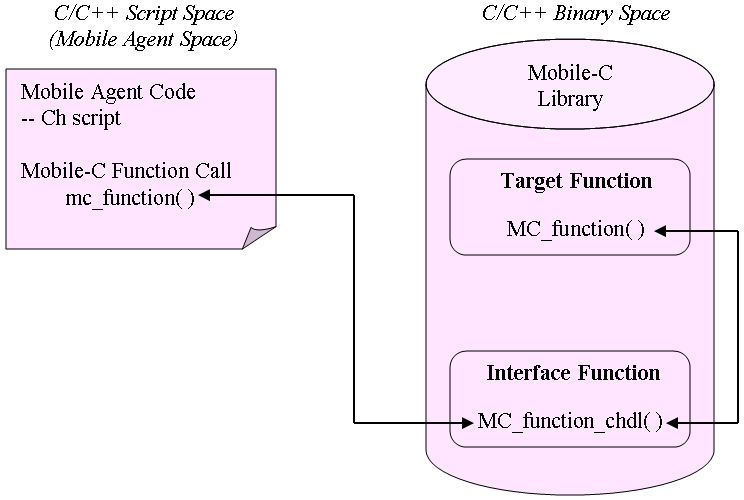
\includegraphics[scale=0.5]{figure/chmobilec_package}
   \caption{Interface of mobile agent code with the Mobile-C library.}
   \label{fig:chmobilec_package}
\end{center}
\end{figure*}
% FIGURE }}}
%%%%%%%%%%%%%%%%%%%%%%%%%%%%%%%%%%%%%%%%%%%%%%%%%%%%%%%%%%%%%%%%%%%%%%
In order to allow mobile agent code to call user defined routines and 
access data sets defined in the binary space, as well as control 
other mobile agents defined in the mobile agent space through the 
Mobile-C API functions, the Mobile-C functionality has to be extended into 
the mobile agent space.
We integrated Ch with the Mobile-C library to provide access to some 
Mobile-C functionalities. 

Figure \vref{fig:chmobilec_package} shows how mobile agent code interfaces 
with the Mobile-C library.
When the function \textit{mc\_function()} is called in mobile agent code,
Ch searches the corresponding interface function \textit{MC\_function\_chdl()} 
in the Mobile-C library, and passes arguments to it by calling the function.
Subsequently, the interface function \textit{MC\_function\_chdl()} invokes the 
target function \textit{MC\_function()}, and passes the return value back to 
the mobile agent space~\cite{EmbeddedCh}.

The prototypes of Mobile-C functions used in the mobile agent space are
declared in \textit{agent.c} through an Embedded Ch function,
\textit{Ch\_DeclareFunc()}.
The data type, \textit{MCAgent\_t}, used as a parameter or return value by 
certain Mobile-C functions for the mobile agent space is also defined in 
\textit{agent.c} by two Embedded Ch functions, 
\textit{Ch\_DeclareVar()} and \textit{Ch\_DeclareTypedef()}~\cite{EmbeddedCh}.
Table \vref{chmobilec_api_cscript} lists the currently implemented functions 
for the mobile agent space.
Two examples are used to demonstrate the applications and features of the 
Mobile-C functionality in the mobile agent space. 

%%%%%%%%%%%%%%%%%%%%%%%%%%%%%%%%%%%%%%%%%%%%%%%%%%%%%%%%%%%%%%%%%%%%%
% Terminate Mobile Agent Execution from Mobile Agent Space {{{
\noindent
\section{Terminate Mobile Agent Execution from Mobile Agent Space}
%%%%%%%%%%%%%%%%%%%%%%%%%%%%%%%%%%%%%%%%%%%%%%%%%%%%%%%%%%%%%%%%%%%%%%
% test2.xml {{{
\begin{Program}[!t]
\begin{center}
   {\footnotesize \linespread{1.0} 
     \verbatiminput{../demos/cspace-agentspace_interface/persistent_example/test2.xml}}
\end{center}
\caption{A mobile agent which enters an infinite loop and does 
  not terminate. \texttt{(<MCPACKAGE>/demos/cspace-agentspace\_interface/persistent\_example/test2.xml)}}
\label{prog:mobileagent1_ex3.xml}
\end{Program}
% }}} test2.xml
%%%%%%%%%%%%%%%%%%%%%%%%%%%%%%%%%%%%%%%%%%%%%%%%%%%%%%%%%%%%%%%%%%%%%%
%%%%%%%%%%%%%%%%%%%%%%%%%%%%%%%%%%%%%%%%%%%%%%%%%%%%%%%%%%%%%%%%%%%%%%
% test3.xml {{{
\begin{Program}[!t]
\begin{center}
   {\footnotesize \linespread{1.0} 
     \verbatiminput{../demos/cspace-agentspace_interface/persistent_example/test3.xml}}
\end{center}
\caption{ This agent terminates the execution
of the agent in Program \ref{prog:mobileagent1_ex3.xml}. 
  \texttt{(<MCPACKAGE>/demos/cspace-agentspace\_interface/persistent\_example/test3.xml)}}
\label{prog:mobileagent2_ex3.xml}
\end{Program}
% }}} test3.xml
%%%%%%%%%%%%%%%%%%%%%%%%%%%%%%%%%%%%%%%%%%%%%%%%%%%%%%%%%%%%%%%%%%%%%%

This example demonstrates how to send a mobile agent to terminate the 
execution of another currently running mobile agent. 
These two mobile agents belong to independent mobile agent spaces. 

The server program used in this example is the same as Program 
\vref{prog:server.c}. 
The client program is the same as Program \vref{prog:client_ex2.c} except 
that it calls the function \textit{MC\_SendAgentMigrationMessageFile()} twice 
to send out two mobile agents.
The first mobile agent sent to the remote agency is 
\textit{test2.xml} shown in Program 
\vref{prog:mobileagent1_ex3.xml}.
The execution of the mobile agent code will repeatedly print a string 
\textit{Hello} to the screen every second.
The second mobile agent sent to the remote agency is 
\textit{test3.xml} shown in Program 
\vref{prog:mobileagent2_ex3.xml}.
The function \textit{mc\_FindAgentByName()} \index{mc\_FindAgentByName()}
returns a variable of type 
\textit{MCAgent\_t} as a handle to a mobile agent. 
The mobile agent code embedded in \textit{mobileagent2\_ex3.xml} finds a 
mobile agent named \textit{mobagent1} by the function 
\textit{mc\_FindAgentByName()} and terminates the execution of 
\textit{mobagent1} by the function \textit{mc\_TerminateAgent()}
\index{mc\_TerminateAgent()}. 
% }}} Terminate Mobile Agent Execution from Mobile Agent Space
%%%%%%%%%%%%%%%%%%%%%%%%%%%%%%%%%%%%%%%%%%%%%%%%%%%%%%%%%%%%%%%%%%%%%%

%%%%%%%%%%%%%%%%%%%%%%%%%%%%%%%%%%%%%%%%%%%%%%%%%%%%%%%%%%%%%%%%%%%%%%
% Invoke a Registered Service from Mobile Agent Space {{{
\noindent
\section{Invoke a Registered Service from Mobile Agent Space}
%%%%%%%%%%%%%%%%%%%%%%%%%%%%%%%%%%%%%%%%%%%%%%%%%%%%%%%%%%%%%%%%%%%%%%
% service_provider_1.xml {{{
\begin{Program}[!t]
\begin{center}
   {\footnotesize \linespread{1.0} 
     \verbatiminput{../demos/agent_space_functionality/mc_df_service_test/service_provider_1.xml}}
\end{center}
\caption{Sample agent containing 'addition' and 'subtraction' services.
Note that the variable ``mc\_current\_agent'' is a special built-in
  variable described in Table
  \vref{tab:agent_space_variables}.\index{mc\_current\_agent}
\texttt{(<MCPACKAGE>/demos/agent\_space\_functionality/mc\_df\_service\_test/ service\_provider\_1.xml)}}
\label{prog:mobileagent1_ex4.xml}
\end{Program}
% }}} service_provider_1.xml
%%%%%%%%%%%%%%%%%%%%%%%%%%%%%%%%%%%%%%%%%%%%%%%%%%%%%%%%%%%%%%%%%%%%%%
%%%%%%%%%%%%%%%%%%%%%%%%%%%%%%%%%%%%%%%%%%%%%%%%%%%%%%%%%%%%%%%%%%%%%%
% service_provider_2.xml {{{
\begin{Program}[!t]
\begin{center}
   {\footnotesize \linespread{1.0} 
     \verbatiminput{../demos/agent_space_functionality/mc_df_service_test/service_provider_2.xml}}
\end{center}
\caption{Sample agent containing 'multiplication' and 'modulus' services.
Note that the variable ``mc\_current\_agent'' is a special built-in
  variable described in Table
  \vref{tab:agent_space_variables}.\index{mc\_current\_agent}
\texttt{(<MCPACKAGE>/demos/mc\_df\_service\_test/service\_provider\_2.xml)}}
\label{prog:mobileagent2_ex4.xml}
\end{Program}
% }}} service_provider_2.xml
%%%%%%%%%%%%%%%%%%%%%%%%%%%%%%%%%%%%%%%%%%%%%%%%%%%%%%%%%%%%%%%%%%%%%%
%%%%%%%%%%%%%%%%%%%%%%%%%%%%%%%%%%%%%%%%%%%%%%%%%%%%%%%%%%%%%%%%%%%%%%
% test2.xml {{{
\begin{Program}[!t]
\begin{center}
   {\scriptsize \linespread{1.0} \verbatiminput{../demos/agent_space_functionality/mc_df_service_test/test1.xml.part1}}
\end{center}
\caption{Sample agent that searches for and invokes agent services.
\texttt{(<MCPACKAGE>/demos/mc\_df\_service\_test/test1.xml)} (Part 1)}
\label{prog:mobileagent3_ex4.xml}
\end{Program}
\addtocounter{Program}{-1}
\begin{Program}[!t]
\begin{center}
   {\scriptsize \linespread{1.0} \verbatiminput{../demos/agent_space_functionality/mc_df_service_test/test1.xml.part2}}
\end{center}
\caption{(Continued) }
\end{Program}
% }}} test2.xml
%%%%%%%%%%%%%%%%%%%%%%%%%%%%%%%%%%%%%%%%%%%%%%%%%%%%%%%%%%%%%%%%%%%%%%

This example demonstrates how to send a mobile agent to invoke a service 
provided by a persistent mobile agent registered with the DF.

The server program used in this example is the same as Program 
\vref{prog:server.c}. 
The client program is the same as Program \vref{prog:client_ex2.c} except 
that it calls the function \textit{MC\_SendAgentMigrationMessageFile()} three
times to send out three mobile agents.
The first mobile agent sent to the remote agency is 
shown in Program 
\vref{prog:mobileagent1_ex4.xml}.
The execution of the mobile agent code will register two services with the 
remote DF through the function mc\_RegisterService(). 
The two services are \textit{addition} and \textit{subtraction} which 
provide addition and subtraction of two integers, respectively.
These services also refer to the functions defined in the mobile agent code.
The function \textit{mc\_RegisterService()} \index{mc\_RegisterService()}
takes three parameters. 
An \textit{MCAgent\_t} type variable is the first parameter. 
A system variable of type \textit{MCAgent\_t}, \textit{mc\_current\_agent}, 
is used as the first parameter when services for 
the current mobile agent are registered, as illustrated in Program 
\vref{prog:mobileagent1_ex4.xml}.
The system variable \textit{mc\_current\_agent} 
is declared in \textit{agent.c} using the function \textit{Ch\_DeclareVar()} 
to hold the current mobile agent.
An array of pointer to char and an integer are the second and third 
parameters, respectively.
The array holds the name of the services whereas the integer denotes the 
number of the services to be registered. 

The second mobile agent is similar to the first and also registers two
services, \textit{multiplication} and \textit{modulus}, which provides 
multiplication and modulo operation of two integers. 
This mobile agent can be seen in Program \vref{prog:mobileagent2_ex4.xml}.

The third mobile agent sent to the remote agency is 
\textit{} shown in Program 
\vref{prog:mobileagent3_ex4.xml}.
The function \textit{mc\_SearchForService()}\index{mc\_SearchForService()} 
takes five parameters.
The first parameter is the name of the service to be found.
The second parameter is the address of an array of ponter to char that 
holds the names of all the mobile agents with the desired service.
Likewise, the third parameter is the address of an array of pointer to 
char that holds the desired service name associated with all the found 
mobile agents.
The fourth parameter is the address of a one-dimensional integer array that 
holds the IDs of all the mobile agents with the desired service.
The last parameter is the address of an integer denoting the number of mobile 
agents that have been found. 
In this example, once the search for \textit{addition} service is done, the 
first mobile agent with this service will be returned by the function 
\textit{mc\_FindAgentByID()}\index{mc\_FindAgentByID()} with a parameter as 
the first element of array \textit{agentIDs}.
In this example, the first found mobile agent is 
\textit{service\_provider\_1}.
The function \textit{addition()} defined in \textit{service\_provider\_1} 
will be called through the function \textit{mc\_CallAgentFunc()} to perform 
addition of two integers.
Since \textit{mc\_CallAgentFunc()}\index{mc\_CallAgentFunc()} can only pass 
one argument to the invoked 
function, the address of a data structure with two integer members is passed 
to \textit{addition()} in this example.
The return value of \textit{addition()} is assigned to the variable 
\textit{retval}.
The string \textit{Result of addition 44 + 45 is 89.} will be printed to the 
screen at the end.   
% }}} Invoke a Mobile Agent Space Function from Mobile Agent Space
%%%%%%%%%%%%%%%%%%%%%%%%%%%%%%%%%%%%%%%%%%%%%%%%%%%%%%%%%%%%%%%%%%%%%%
% }}} Extend Mobile-C Functionality to Mobile Agent Space
%%%%%%%%%%%%%%%%%%%%%%%%%%%%%%%%%%%%%%%%%%%%%%%%%%%%%%%%%%%%%%%%%%%%%%

%%%%%%%%%%%%%%%%%%%%%%%%%%%%%%%%%%%%%%%%%%%%%%%%%%%%%%%%%%%%%%%%%%%%%%
% Synchronization Support int he Mobile-C Library {{{
\chapter{\label{chap:synchronization}Synchronization Support in the Mobile-C library}
In a Mobile-C agency, mobile agents are executed by independent AEEs. 
A user might also need to design a multi-threaded application where a Mobile-C 
agency itself is one of the many threads that handle different tasks.
The Mobile-C library provides support for synchronization among mobile 
agents and threads.
The synchronization API functions are used to protect shared resources as well 
as provide a method of deterministically timing the execution of mobile agents 
and threads.

The internal implementation consists of a linked list of 
Portable Operating System Interface for UNIX (POSIX) compliant synchronization 
variables, namely, mutexes, condition variables, and semaphores. 
Each node in the linked list is a synchronization variable which is assigned 
or given a unique identification number. 
The API functions can be called from the binary or mobile agent 
space to initialize the synchronization variables and access them by their 
unique identification numbers in the linked list.

A Mobile-C synchronization variable is an abstract variable, initialized
by the function {\it MC\_SyncInit()} \index{MC\_SyncInit()}\index{mc\_SyncInit()}.
Once it has been initialized, it may be used as a mutex, condition variable, 
or semaphore.
No further function calls are necessary to change a generic synchronization
variable to one of the types. However, once a synchronization variable is
used as a mutex, condition variable, or semaphore, it should not be used again
as a different type. For instance, if calls to 
\begin{verbatim}
MC_SyncInit(500);
MC_MutexLock(500);
\end{verbatim}
are made, initializing a synchronization variable with ID ``500'', and locking
it as a mutex, it should not be then used with any of the condition variable or
semaphore functions.

The application of the Mobile-C synchronization mechanism is illustrated by 
the example below.

%%%%%%%%%%%%%%%%%%%%%%%%%%%%%%%%%%%%%%%%%%%%%%%%%%%%%%%%%%%%%%%%%%%%%%
% Synchronization in Mobile Agent Space {{{
\noindent
\section{Synchronization in Mobile Agent Space}
%%%%%%%%%%%%%%%%%%%%%%%%%%%%%%%%%%%%%%%%%%%%%%%%%%%%%%%%%%%%%%%%%%%%%%
% client.c {{{
\begin{Program}[!t]
\begin{center}
   {\footnotesize \linespread{1.0} 
     \verbatiminput{../demos/synchronization/agent_mutex_example/client.c}}
\end{center}
\caption{A program used to send a mobile agent. 
  \texttt{(<MCPACKAGE>/demos/synchronization/ agent\_mutex\_example/mc\_client.c)}}
\label{prog:client_ex5.c}
\end{Program}
% }}} client.c
%%%%%%%%%%%%%%%%%%%%%%%%%%%%%%%%%%%%%%%%%%%%%%%%%%%%%%%%%%%%%%%%%%%%%%
%%%%%%%%%%%%%%%%%%%%%%%%%%%%%%%%%%%%%%%%%%%%%%%%%%%%%%%%%%%%%%%%%%%%%%
% sleep.xml {{{
\begin{Program}[!t]
\begin{center}
   {\footnotesize \linespread{1.0} 
     \verbatiminput{../demos/synchronization/agent_mutex_example/sleep.xml}}
\end{center}
\caption{An agent which uses a mutex while accessing a shared resource.
  \texttt{(<MCPACKAGE>/demos/synchronization/agent\_mutex\_example/sleep.xml)} }
\label{prog:mobileagent1_ex5.xml}
\end{Program}
% }}} sleep.xml
%%%%%%%%%%%%%%%%%%%%%%%%%%%%%%%%%%%%%%%%%%%%%%%%%%%%%%%%%%%%%%%%%%%%%%
%%%%%%%%%%%%%%%%%%%%%%%%%%%%%%%%%%%%%%%%%%%%%%%%%%%%%%%%%%%%%%%%%%%%%%
% wake.xml {{{
\begin{Program}[!t]
\begin{center}
   {\footnotesize \linespread{1.0} \verbatiminput{../demos/synchronization/agent_mutex_example/wake.xml}}
\end{center}
\caption{An agent which uses a mutex while accessing a shared resource.
  \texttt{(<MCPACKAGE>/demos/synchronization/agent\_mutex\_example/wake.xml)} }
\label{prog:mobileagent2_ex5.xml}
\end{Program}
% }}} wake.xml
%%%%%%%%%%%%%%%%%%%%%%%%%%%%%%%%%%%%%%%%%%%%%%%%%%%%%%%%%%%%%%%%%%%%%%

The Mobile-C library allows synrchonization among agents via
mutexes, condition variables, and semaphores. Each type of synchronization
variable is used for different features. Perhaps the most common and basic
of these variables is the mutex.

The client program shown in Program \vref{prog:client_ex5.c} starts a Mobile-C
agency listening on port \textit{5050} and subsequently sends two mobile 
agents to 
the remote agency running on host \textit{localhost} at port 
\textit{5051}.
The mobile agents are shown in Program \vref{prog:mobileagent1_ex5.xml} 
and Program \vref{prog:mobileagent2_ex5.xml}. These mobile agents will use
a mutex to guard an operation that may not be performed by two agents
simultaneously.

This example demonstrates the ability of a Mobile-C mutex to protect
a resource that may be shared between two agents. Any real or
imaginary resource that should
not be accessed simultaneously by more than one entity at a time should
be guarded by a mutex. The resource may be a shared variable, or something
more abstract such as control of a robot arm. If there is only one robot arm,
then only one entity, an agent in this case, should be able to control it at a 
time.

In our particular example, the tasks our agents are going to perform are
imaginary. Each task is represented instead by the ``sleep()'' function and
the printing of a message,
which causes execution of that particular agent to pause for a time, as
if it were performing a task. For our example, we will intentionally
cause our agents to collide execution times to demonstrate that our 
mutex works. Examining our client program, Program 
\vref{prog:client_ex5.c},
we see that we set a two second interval between sending the agents. However,
the task that each agent tries to perform will be five seconds long. This
means that the second agent will arrive while the first agent is in the middle
of performing its simulated task. The execution output will demonstrate that
the second agent will not begin its task until the first agent is finished.

Semaphores are also used to guard resources in which a limited number of
entities may access at a time. Since the behaviour and usage of semaphores are
similar to that of a mutex, an example is not provided here. Please see
the demo in directory \texttt{<MCPACKAGE>/demos/agent\_semaphore\_example/} for an example.

\begin{Program}[!t]
\begin{center}
   {\footnotesize \linespread{1.0} \verbatiminput{../demos/synchronization/agent_cond_example/sleep.xml}}
\end{center}
\caption{A sample agent which will immediately sleep on a condition variable
after arriving at an agency. \texttt{(<MCPACKAGE>/demos/synchronization/agent\_cond\_example/sleep.xml)}}
\label{prog:cond_agent_1}
\end{Program}

\begin{Program}[!t]
\begin{center}
   {\footnotesize \linespread{1.0} \verbatiminput{../demos/synchronization/agent_cond_example/wake.xml}}
\end{center}
\caption{A sample agent which will signal a condition variable after arriving
at an agency. \texttt{(<MCPACKAGE>/demos/synchronization/agent\_cond\_example/wake.xml)}}
\label{prog:cond_agent_2}
\end{Program}

Condition variables are also useful in multi-threaded applications in order
for threads to sleep and wait for a signal. Program 
\vref{prog:cond_agent_1} illustrates an agent that will sleep on a condition
  variable immediately after arriving at an agency. Program 
\vref{prog:cond_agent_2} shows an agent that will send a signal to the condition
variable the first agent in Program \ref{prog:cond_agent_1} is waiting on, thereby
causing the first agent to wake up and continue execution.
% }}} Synchronization in the Mobile Agent Space 
%%%%%%%%%%%%%%%%%%%%%%%%%%%%%%%%%%%%%%%%%%%%%%%%%%%%%%%%%%%%%%%%%%%%%%

%%%%%%%%%%%%%%%%%%%%%%%%%%%%%%%%%%%%%%%%%%%%%%%%%%%%%%%%%%%%%%%%%%%%%%
% Synchronization Between Binary and Agent Spaces {{{
%%%%%%%%%%%%%%%%%%%%%%%%%%%%%%%%%%%%%%%%%%%%%%%%%%%%%%%%%%%%%%%%%%%%%%
% server.c {{{
\begin{Program}[!t]
\begin{center}
   {\footnotesize \linespread{1.0} \verbatiminput{../demos/synchronization/cspace_mutex_example/server.c}}
\end{center}
\caption{A sample program with an embedded Mobile-C agency demonstrating the use of a 
Mobile-C mutex to protect a shared resource. \texttt{(<MCPACKAGE>/demos/synchronization/cspace\_mutex\_example/mc\_server.c)}}
\label{prog:binary_sync_example_server}
\end{Program}
% }}} server.c
%%%%%%%%%%%%%%%%%%%%%%%%%%%%%%%%%%%%%%%%%%%%%%%%%%%%%%%%%%%%%%%%%%%%%%

%%%%%%%%%%%%%%%%%%%%%%%%%%%%%%%%%%%%%%%%%%%%%%%%%%%%%%%%%%%%%%%%%%%%%%
% agent.xml {{{
\begin{Program}[!t]
\begin{center}
   {\footnotesize \linespread{1.0} \verbatiminput{../demos/synchronization/cspace_mutex_example/agent.xml}}
\end{center}
\caption{A sample Mobile-C agent which must perform an action on a shared resource
guarded by a Mobile-C mutex. \texttt{(<MCPACKAGE>/demos/synchronization/cspace\_mutex\_example/agent.xml)}}
\label{prog:binary_sync_example_agent}
\end{Program}
% }}} agent.xml
%%%%%%%%%%%%%%%%%%%%%%%%%%%%%%%%%%%%%%%%%%%%%%%%%%%%%%%%%%%%%%%%%%%%%%

\section{Synchronization Between Binary and Agent Spaces}
The synchronization variables initialized using MC\_SyncInit() are accessible
in both agent space and binary space, enabling agents to synchronize with 
binary threads. Again, all three Mobile-C synchronization variable types:
mutexes, condition variables, and semaphores, may be used in both
binary and agent space. 

Referring the example server code in Program
\vref{prog:binary_sync_example_server}, we show a piece of code where
a binary program containing a Mobile-C agency must perform a
subroutine involving a shared resource, protecting it with a mutex. 
The shared resource will
be accessible from both the main() binary thread as well as any agents
which are residing in the agency. As such, the server code 
initializes and uses a mutex to protect the shared resource. In our 
example agent shown in Program \vref{prog:binary_sync_example_agent},
we see that this agent needs to access the same shared resource,
and so it must first lock the mutex before doing so. This example
demonstrates that the mutex will prevent both the agent and binary
thread from accessing the resource simultaneously

%%%%%%%%%%%%%%%%%%%%%%%%%%%%%%%%%%%%%%%%%%%%%%%%%%%%%%%%%%%%%%%%%%%%%%
% server.c {{{
\begin{Program}
\begin{center}
   {\footnotesize \linespread{1.0} \verbatiminput{../demos/synchronization/cspace_cond_example/server.c}}
\end{center}
\caption{An example server containing a thread which will run once each time it
is signalled by another thread or by an agent. 
  \texttt{(<MCPACKAGE>/demos/synchronization/cspace\_cond\_example/mc\_server.c)}}
\label{prog:binary_cond_example_server}
\end{Program}
% }}} server.c
%%%%%%%%%%%%%%%%%%%%%%%%%%%%%%%%%%%%%%%%%%%%%%%%%%%%%%%%%%%%%%%%%%%%%%

%%%%%%%%%%%%%%%%%%%%%%%%%%%%%%%%%%%%%%%%%%%%%%%%%%%%%%%%%%%%%%%%%%%%%%
% agent.xml {{{
\begin{Program}
\begin{center}
   {\footnotesize \linespread{1.0} \verbatiminput{../demos/synchronization/cspace_cond_example/agent.xml}}
\end{center}
\caption{A sample agent which signals a condition variable.
\texttt{(<MCPACKAGE>/demos/synchronization/cspace\_cond\_example/agent.xml)}}
\label{prog:binary_cond_example_agent}
\end{Program}
% }}} agent.xml
%%%%%%%%%%%%%%%%%%%%%%%%%%%%%%%%%%%%%%%%%%%%%%%%%%%%%%%%%%%%%%%%%%%%%%

Referring now to 
Program \vref{prog:binary_cond_example_server} and Program 
\vref{prog:binary_cond_example_agent}, we demonstrate the use of 
Mobile-C condition variables to synchronize an agent with a binary thread.
The binary space thread program shown in Program \ref{prog:binary_cond_example_server}
simply waits on a condition variable. The agent shown in Program
\ref{prog:binary_cond_example_agent} signals the binary space thread
with a call to {\it mc\_CondSignal()}, causing the binary space
thread to run once. 
% }}} Synchronization Between Binary and Agent Spaces
%%%%%%%%%%%%%%%%%%%%%%%%%%%%%%%%%%%%%%%%%%%%%%%%%%%%%%%%%%%%%%%%%%%%%%

%%%%%%%%%%%%%%%%%%%%%%%%%%%%%%%%%%%%%%%%%%%%%%%%%%%%%%%%%%%%%%%%%%%%%%
% Mobile-C Execution with Multiple Agencies {{{
\section{Mobile-C Execution with Multiple Agencies}
%%%%%%%%%%%%%%%%%%%%%%%%%%%%%%%%%%%%%%%%%%%%%%%%%%%%%%%%%%%%%%%%%%%%%%
% server.c {{{
\begin{Program}[!t]
\begin{center}
   {\footnotesize \linespread{1.0} \verbatiminput{../demos/miscellaneous/multiple_agency_example/server.c}}
\end{center}
\caption{An example program containing two Mobile-C agencies. The program
copies agents arriving at the agency on port 5051 to the agency at port
5052.\texttt{(<MCPACKAGE>/demos/miscellaneous/multiple\_agency\_example/mc\_server.c)}}
\label{prog:multiple_agency_server}
\end{Program}
% }}} server.c
%%%%%%%%%%%%%%%%%%%%%%%%%%%%%%%%%%%%%%%%%%%%%%%%%%%%%%%%%%%%%%%%%%%%%%

Using the Mobile-C library, multiple agencies may be initialized 
within the same program. This is useful in cases where the agencies
may have different AEE configuration properties, privileges, etc. 
Ch is the chosen AEE of Mobile-C. 
Functions such as MC\_CopyAgent() and MC\_AddAgent() become useful
in such cases. 

In the example shown in Program \vref{prog:multiple_agency_server},
we demonstrate a program with two agencies, listening on ports
5051 and 5052, respectively. In our simple example, the server
simple duplicates every agent arriving to the agency on port 5051
and adds a copy to the agency on port 5052. 

Note that the 
MC\_CopyAgent() function is necessary here because Mobile-C
functions which retrieve agents from agencies only retrieve references
to the agents, not copies of the agents. The MC\_CopyAgent() function performs
a deep copy on the agent structure so that it may be used in another
agency. Also note that setting the copied agent's status to 
``MC\_WAIT\_CH'' ensures that it will execute again upon entering the 
second agency. 
% }}} Mobile-C Execution with Multiple Agencies
%%%%%%%%%%%%%%%%%%%%%%%%%%%%%%%%%%%%%%%%%%%%%%%%%%%%%%%%%%%%%%%%%%%%%%

% }}} Synchronization Support in the Mobile-C Library
%%%%%%%%%%%%%%%%%%%%%%%%%%%%%%%%%%%%%%%%%%%%%%%%%%%%%%%%%%%%%%%%%%%%%%

%%%%%%%%%%%%%%%%%%%%%%%%%%%%%%%%%%%%%%%%%%%%%%%%%%%%%%%%%%%%%%%%%%%%%%
% {{{ Mobile-C Security Module
\chapter{Mobile-C Security Module \label{chap:Security}}
The Mobile-C package (version 1.10.@@) includes a security module. 
This security module is intended to provide secure migration process of 
  mobile agents and ACL messages from one agency to another. 
Before the migration process, both agencies must authenticate each other 
  successfully. 
After that, an encrypted mobile agent is transferred and its integrity 
  is verified at the receiver side. 
The security module helps guard against man-in-the-middle attacks and
  eavesdropping, and provides a strong authentication of the 
  agencies involved in the migration process.

%%%%%%%%%%%%%%%%%%%%%%%%%%%%%%%%%%%%%%%%%%%%%%%%%%%%%%%%%%%%%%%%%%%%%%
% Security Module Architecture and Overview {{{
\section{Security Module Architecture and Overview}
The Mobile-C security module is inspired by the SSH protocol.
When a security-enabled agency attempts to contact another agency for 
  the migration of a mobile agent or an ACL message, both
  agencies must authenticate each other before the  migration process. 
A successful authentication creates a trust between the two agencies.

Each security-enabled agency must contain a \textit{known\_host} file 
  and a pair of private (\textit{rsa\_priv}) and public (\textit{rsa\_pub}) 
  key files.
These files are provided to each agency by the administrator at 
  startup time. 
The \textit{known\_host} file contains the host name and public key 
  of each agency in the network, as an identifier. 
By default, each agency trusts all the agencies that are listed 
  in the \textit{known\_host} file. 
The \textit{rsa\_priv} and \textit{rsa\_pub} key files contains the 
  private and public key of the agency.

% }}} Security Module Architecture and Overview
%%%%%%%%%%%%%%%%%%%%%%%%%%%%%%%%%%%%%%%%%%%%%%%%%%%%%%%%%%%%%%%%%%%%%%


%%%%%%%%%%%%%%%%%%%%%%%%%%%%%%%%%%%%%%%%%%%%%%%%%%%%%%%%%%%%%%%%%%%%%%
% Enabling the Security Module {{{
\section {Enabling the Security Module}
The configuration options need to be changed in order for the module 
to be built and used are below.
%%%%%%%%%%%%%%%%%%%%%%%%%%%%%%%%%%%%%%%%%%%%%%%%%%%%%%%%%%%%%%%%%%%%%%
% Enabling the Security Module in Unix {{{
\subsection{Enabling the Security Module in Unix}
In a Unix environment, a configuration option needs to be stated during
the configuration process. The new configuration step will be the command
\begin{verbatim}
./configure --enable-security
\end{verbatim}
instead of the old
\begin{verbatim}
./configure
\end{verbatim}

% }}} Enabling the Security Module in Unix
%%%%%%%%%%%%%%%%%%%%%%%%%%%%%%%%%%%%%%%%%%%%%%%%%%%%%%%%%%%%%%%%%%%%%%

%%%%%%%%%%%%%%%%%%%%%%%%%%%%%%%%%%%%%%%%%%%%%%%%%%%%%%%%%%%%%%%%%%%%%
% Enabling the Security Module in Windows {{{
\subsection{Enabling the Security Module in Windows}
For Windows, below is the line that needs to be comment out in the 
file ``[MobileC\_HOME]/src/winconfig.h''.
\begin{verbatim}
#define MC_SECURITY 1
\end{verbatim}
% }}} Enabling the Security Module in Windows
%%%%%%%%%%%%%%%%%%%%%%%%%%%%%%%%%%%%%%%%%%%%%%%%%%%%%%%%%%%%%%%%%%%%%%

%%%%%%%%%%%%%%%%%%%%%%%%%%%%%%%%%%%%%%%%%%%%%%%%%%%%%%%%%%%%%%%%%%%%%%
% Further Instructions {{{
\subsection{Further Instructions}
If the private key file is used in encrypted form then option needs to 
be turned on. 
The following C code snippet will start a security-enabled agency 
  listening on port 5050.
\begin{verbatim}
MCAgency_t agency;
MC_AgencyOptions_t options;
MC_InitializeAgencyOptions(&options);
strcpy(options.passphrase, "alpha1234");
agency = MC_Initialize(5050, &options);

\end{verbatim}

See more about the MC\_AgencyOptions\_t type at the description of the
  MC\_Initialize() function in Appendix A on page \pageref{api:MC_Initialize}.

% }}} Further Instructions
%%%%%%%%%%%%%%%%%%%%%%%%%%%%%%%%%%%%%%%%%%%%%%%%%%%%%%%%%%%%%%%%%%%%%%

% }}} Enabling the Security Module
%%%%%%%%%%%%%%%%%%%%%%%%%%%%%%%%%%%%%%%%%%%%%%%%%%%%%%%%%%%%%%%%%%%%%%

%%%%%%%%%%%%%%%%%%%%%%%%%%%%%%%%%%%%%%%%%%%%%%%%%%%%%%%%%%%%%%%%%%%%%%
% Preparation to Run Security Enabled Agency  {{{
\section{Preparation to Run Security Enabled Agency}
Before running a Mobile-C agency with the security option, 
  the following files are required.
\begin{enumerate}
\item A known host file (\text{known\_host})
\item A pair for public (\textit{rsa\_pub}) and private 
      (\textit{rsa\_priv}) key files
\end{enumerate} 
  are required to be created. 
These are \textit{known\_host} file and \textit{private key} file.  
A small utility source program 
  \begin{verbatim} [MobileC-SRC_HOME]/src/util/mc_keygen.c \end{verbatim} 
  is provided with the Mobile-C library to create a pair of public 
  and private key files for an agency. 
When you make the Mobile-C library the executable for this source program
  can be found in 
  \begin{verbatim} [Mobile-C_HOME]/bin/mc_keygen \end{verbatim}
It is required to create a separate pair of public and private key file
  for each agency. 
That means if there are \textit{n} agencies in a network then \textit{n}
  number of public and private key file pairs are required.
The private key files can be created in plaintext or encrypted 
  form. Details can be found in section 9.3.1.
The known host file needs to be built manually after creating public
  and private key files.

%%%%%%%%%%%%%%%%%%%%%%%%%%%%%%%%%%%%%%%%%%%%%%%%%%%%%%%%%%%%%%%%%%%%%%
% Generating Key Files {{{
\subsection{Generating Key Files}
A utility program {\bf mc\_genkey} \textit{([MobileC-Home]/bin/mc\_genkey)} is 
used to create public and private key files.
This utility program can create a private key in plain text or cipher text.
To generate the key files with private key in plain text, you can execute the 
{\bf mc\_genkey} as 
\begin{verbatim}
$./mc_genkey -rsakeys -pt
Seeding the random number generator 
Generating the RSA key [ 1024-bit ] 
Exporting public key in rsa_pub 
Exporting the private key in rsa_priv 
Done. 
Key generated.
\end{verbatim}
where \textit{-pt} means to generate private key in plain text. 
Similarly,
\begin{verbatim}
$./mc_genkey -rsakeys -en
Enter Passphrase (A-Z, a-z, 0-9)to encrypt privatekey file
(remember your passphrase otherwise encrypted private key file is useless)
>  alpha1234

Seeding the random number generator 
Generating the RSA key [ 1024-bit ] 
Exporting public key in rsa_pub 
Exporting the private key in rsa_priv 
encrypted. 
done. 
keys generated.
\end{verbatim}

would generate the private key in encrypted form, where \textit{en} stands 
for encryption. 
Here we a passphrase (\textit{alpha1234})is provided to encrypt the private 
  key file. 
With this option it prompts for the passphrase that is used to encrypt the 
  rsa private key. 
Here we entered a passphrase (\textit{alpha1234}) to encrypt the private 
  key file.
You can enter a string maximum upto 32 bytes in length consisting of small 
  or capital alphabet and/or 1-9 digits. 
The same passphrase is required by the Mobile-C agency to decrypt the 
  private key file.
With both options, it generates the public key file in plain text.
The output file names are \textit{rsa\_pub} for public key and
\textit{rsa\_priv} for private key.

% }}} Generating Key Files
%%%%%%%%%%%%%%%%%%%%%%%%%%%%%%%%%%%%%%%%%%%%%%%%%%%%%%%%%%%%%%%%%%%%%%

%%%%%%%%%%%%%%%%%%%%%%%%%%%%%%%%%%%%%%%%%%%%%%%%%%%%%%%%%%%%%%%%%%%%%%
% FIGURE {{{ 
\begin{figure*}[!t]
\begin{center}
   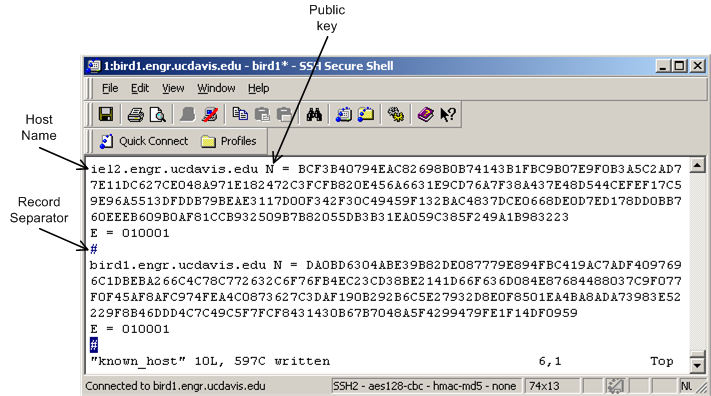
\includegraphics[scale=0.5]{figure/knownhost}
   \caption{A sample known host file.}
   \label{fig:knownhost}
\end{center}
\end{figure*}
% FIGURE }}}
%%%%%%%%%%%%%%%%%%%%%%%%%%%%%%%%%%%%%%%%%%%%%%%%%%%%%%%%%%%%%%%%%%%%%%

%%%%%%%%%%%%%%%%%%%%%%%%%%%%%%%%%%%%%%%%%%%%%%%%%%%%%%%%%%%%%%%%%%%%%%
% Known Host file {{{
\subsection{Known Host File}
After creating the key files for all the agencies in a network the 
  \textit{known\_host} file needs to be created manully.
The sample \textit{known\_host} file is shown in Figure ~\ref{fig:knownhost}. 
To proceed, create a file using a text editor with name 
  \textit{known\_host}. 
Type the name of the first agency (as shown \textit{Host Name} in 
Figure ~\ref{fig:knownhost}) and 
copy its public key from \textit{rsa\_pub} file. Insert the record 
separation character \# and type the same for second agency and continue.
Make sure that the name for the \textit{known\_host} file is 
\textit{``known\_host"}. After creating the 
\textit{known\_host} file, copy the \textit{known\_host} file to each \
agency and the \textit{rsa\_priv} file on the respective
agencies (the same directory from where you will run the Mobile-C 
agency). 
Public and private key files are always created as a pair this means that
  any text encrypted with the public key can only be decrypted with the
  corresponding (paired) private key.
Therefore, please make sure that the copied private key 
(\textit{rsa\_priv}) to an agency must correspond to the public key
that is mentioned infront of the name of this agency in \textit{
known\_host} file.
% }}} Known Host File
%%%%%%%%%%%%%%%%%%%%%%%%%%%%%%%%%%%%%%%%%%%%%%%%%%%%%%%%%%%%%%%%%%%%%%

%}}} Preparation to Run Security Enabled Agency
%%%%%%%%%%%%%%%%%%%%%%%%%%%%%%%%%%%%%%%%%%%%%%%%%%%%%%%%%%%%%%%%%%%%%

%%%%%%%%%%%%%%%%%%%%%%%%%%%%%%%%%%%%%%%%%%%%%%%%%%%%%%%%%%%%%%%%%%%%%
% Examples {{{
\section{Examples -- Mobile-C Security}
A Mobile-C security enable agency can be executed with encypted or plaintext
  private key. 
When you execute a Mobile-C agency it will look for private key file named
  \textit{rsa\_priv} in the current directory. 
If the private key is encrypted and the passphrase is not provided in Mobile-C
  agency C program then it will prompt for the passphrase.
\texttt{<MCPACKAGE>/demos/} contains two demos 
  (\textit{hello\_world\_secure} and \textit{multi\_task\_example\_secure}) that 
  uses private key in plain text.

Please note that for \textit{hello\_world\_secure} demo, the private and public
  key pair is same for client and server, that is both the client and server 
  program run on the same machine (iel2.engr.ucdavis.edu).
To run the demo in your machine, you to write the name of your machine in 
  \textit{known\_host} file and the mobile agent file (\textit{test1.xml}) 

To run client and server agencies on the two different machines, you need to
  create a pair of public and private keys (see section 9.3.1) and that 
  is for the second machine.  
The first agency can use the already created key files that are provided with
  demos.
After creating the key files, edit the \textit{known\_host} file by including
  the name of other machine and newly created public key from file 
  (\textit{rsa\_priv}), for details see section 9.3.2.
Also copy the newly generated private key file (\textit{rsa\_priv}) and 
  updated \textit{known\_host} file on the other machine in the same 
  directory from where Mobile-C agency will be executed.
Now start the server program and then the client program.

Please note that when you build the demos, the executable 
 files ( \textit{client} and  \textit{server}) for demo 
 \textit{hello\_world \_secure} are in 
 directories \textit{hello\_world\_secure/client} and 
 \textit{hello\_world\_ secure/server} respectively. Similarly, the executable 
 files (\textit{client},  \textit{server1} and  \textit{server2} ) for demo
  \textit{multi\_task\_example\_secure} are in directories 
   \textit{multi\_task\_e xample\_secure/client}, 
   \textit{multi\_task\_example\_secure/server1} and
   \textit{multi\_task\_example\_secure/server2} respectively.

Each agency uses a separate \textit{known\_host},
  public(\textit{rsa\_pub}) and private key {\textit{rsa\_priv} pair files. 

\begin{Program}[!t]
\begin{center}
   {\footnotesize \linespread{1.0} \verbatiminput{../demos/mobilec_security/hello_world_secure/server.c }}
\end{center}
\caption{ A sample server side code for security enable agency 
       (\textit{../demos/mobilec\_security/hello\_world\_secure/server.c})}
\label{prog:security_server}
\end{Program}

\begin{Program}[!t]
\begin{center}
   {\footnotesize \linespread{1.0} \verbatiminput{../demos/mobilec_security/hello_world_secure/client.c }}
\end{center}
\caption{ A sample client side code for security enable agency
        (\textit{../demos/mobilec\_security/hello\_world\_secure/client.c})}
\label{prog:security_client}
\end{Program}

The programs \ref{prog:security_server} and \ref{prog:security_client} show 
  \textit{hello\_world\_secure} server and client code respectively.
Please note that the \textit{MC\_AgencyOptions\_t} is required only if the 
  private key file is encrypted. 
Since both programs use the private key file (\textit{rsa\_priv}) in plaintext
  so \textit{MC\_AgencyOptions\_t} is NULL in \textit{MC\_Initialize} function.

If you generate the private key file (\textit{rsa\_priv}) in encrypted form 
   (see section 9.3.1) then the Mobile-C agency requires the same passphrase 
    to decrypt its private key that you have entered to encrypted this file.
In this case \textit{MC\_AgencyOptions\_t} should not be NULL. 
It is a possible that passphrase would not be privided in the code. 
That is, this code can be run if 
  \textit{strcpy(options.passphrase, "xxxx");} is commented out.
In this case, if the private key is encyrpted the Mobile-C agency
  would prompt to enter passphrase at startup otherwise not. 

%To run the these programs in your machine you need to replace 
%  \textit{rabbit.engr.ucdavis.edu} to your machine name in 
%  \textit{client.c}, \textit{test1.xml} and \textit{known\_host}
%  file.
%The \textit{test1.xml} is a hello world mobile agent. \
     

% }}} Example


%%%%%%%%%%%%%%%%%%%%%%%%%%%%%%%%%%%%%%%%%%%%%%%%%%%%%%%%%%%%%%%%%%%%%%

% }}} Mobile-C Security Module
%%%%%%%%%%%%%%%%%%%%%%%%%%%%%%%%%%%%%%%%%%%%%%%%%%%%%%%%%%%%%%%%%%%%%%

%%%%%%%%%%%%%%%%%%%%%%%%%%%%%%%%%%%%%%%%%%%%%%%%%%%%%%%%%%%%%%%%%%%%%%
%{{{Communication With Other FIPA Compliant Agent Systems
\chapter{Communication With Other FIPA Compliant Agent Systems}
This section provides some brief examples regarding communication
between Mobile-C and other FIPA compliant agent systems.
\subsection{Example: Receiving a message from a JADE agent}
The following section contains details regarding an example where a
Mobile-C agent receives a message from a JADE agent. This example is
included to provide a brief overview of how FIPA ACL communication
operates between Mobile-C agencies and JADE agencies.

\subsubsection{Start a Mobile-C Agency}
The first step in the example is to start a Mobile-C agency and a suitable
agent to wait for a message. An example agency which performs these tasks
may be found in the directory \texttt{<MCPACKAGE>/demos/ jade\_to\_mc\_example/}.
To start the agency, simply go to the directory and execute the server
with the command
\begin{verbatim}
./server
\end{verbatim}
The server will start and load the sample agent named ``mobagent1'' in one step,
which should produce the following output (or similar):
\begin{verbatim}
Mobile-C Started

MobileC > This is mobagent1 from the agency at port 5050.
Now, I am going to wait until I receive a message. Waiting...
\end{verbatim}

\subsubsection{Create a JADE container}
The next step is to start a JADE agency. Instructions on how to obtain and
install JADE may be found at the website \texttt{<http://jade.tilab.com>} .
Once JADE in installed, use the command
\begin{verbatim}
java jade.Boot -gui
\end{verbatim}
to start a JADE container. Note that the command may vary across systems depending
on your java distribution and system setup. This command should produce a window
similar to the following:

\begin{center}
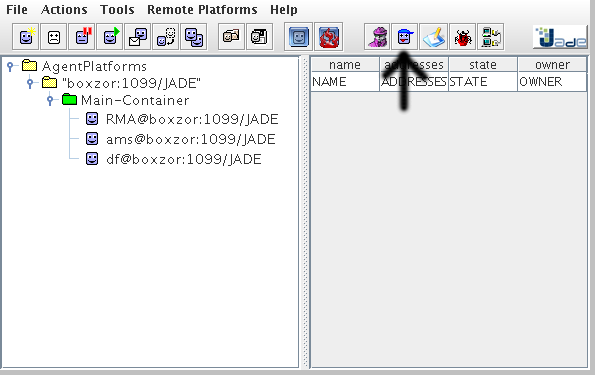
\includegraphics[width=4in]{figure/jade_to_mc_example/jade_main_window.png}
\end{center}

\subsubsection{Start a JADE dummy agent}
The next step is to start a ``dummy'' agent by clicking on the button indicated by the 
large arrow in the previous figure. This should produce a second window
which should resemble the following image.

\begin{center}
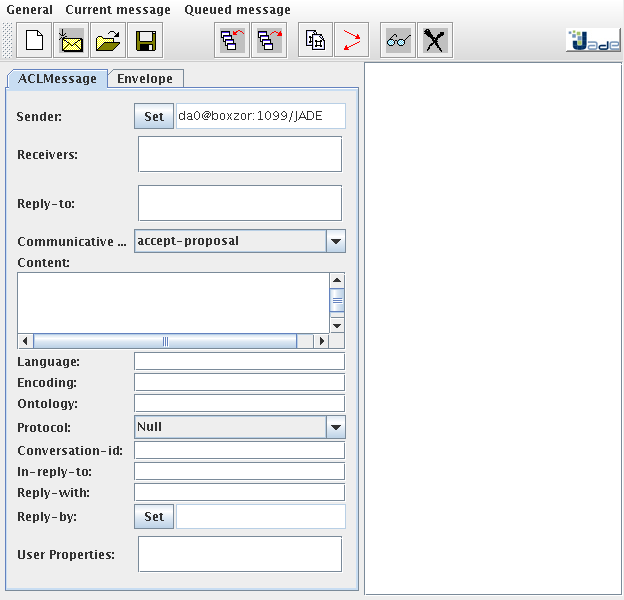
\includegraphics[width=4in]{figure/jade_to_mc_example/dummy_agent_window_blank.png}
\end{center}

\subsubsection{Send a message to Mobile-C}
There are several fields in this empty ACL message that need to be set before the
message will be successfully passed to our Mobile-C agent. The first field to fill
out is the \texttt{Receivers}, which indicates the recipients for our message.
We wish for our Mobile-C agent ``mobagent1'' to be our sole recipient. Add 
``mobagent1'' by right-clicking on the \texttt{Receivers} textbox and selecting the
\texttt{Add} option. Fill out the box as shown in the following image:

\begin{center}
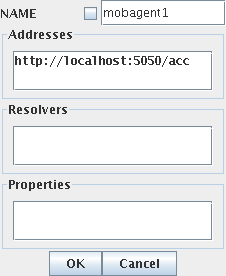
\includegraphics[width=2in]{figure/jade_to_mc_example/dummy_agent_receiver_window.png}
\end{center}

After setting the receiver, the rest of the message may be set to whatever is desired.
For this example, our sample message may be seen on the following image.

\begin{center}
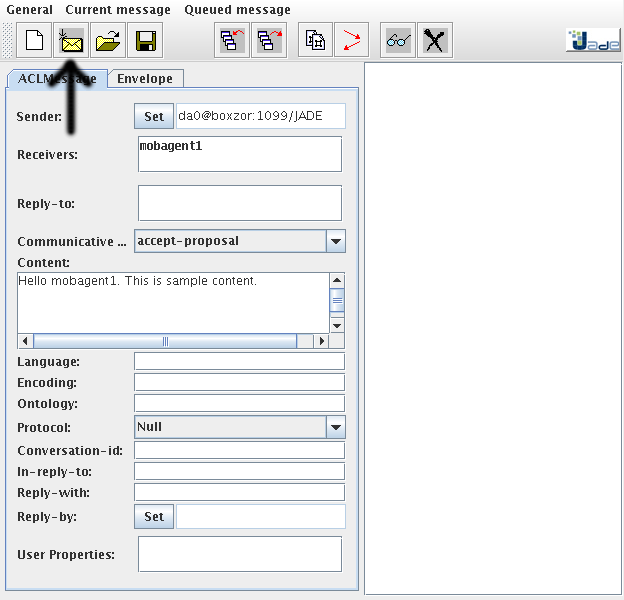
\includegraphics[width=4in]{figure/jade_to_mc_example/dummy_agent_window_complete.png}
\end{center}

Once your desired message parameters are in place, click on the ``Send Message'' button
indicated by the arrow in the previous figure. The message will be sent to the agent
waiting at the Mobile-C agency that was previously started. The agent should
receive the message and produce the following output:
\begin{verbatim}
mobagent1 Got a message!
Message is from da0@boxzor:1099/JADE
The content is Hello mobagent1. This is sample content.
\end{verbatim}
This indicates that \texttt{mobagent1} has successfully received the
message from JADE.

\subsection{Example: Sending a message from Mobile-C to JADE}
This example illustrates a Mobile-C agent sending an ACL message to a
JADE agent.  The example will be presented in a step by step fashion and all
files may be found in the directory \texttt{<MCPACKAGE>/demos/mc\_to\_jade\_example/}.

\subsubsection{Start a JADE container with a ``PingAgent'' agent}
The first step is to start a JADE container with a responsive agent. In this
example, we will use a demo ``PingAgent'' agent which is provided with JADE. The
agent source code may be found in the JADE subdirectory 
\texttt{jade/src/examples/PingAgent/PingAgent.java} . After installing JADE,
run the command
\begin{verbatim}
java jade.Boot pingme:examples.PingAgent.PingAgent
\end{verbatim}
from the \texttt{jade/src/} directory to start a JADE main container and 
invoke an agent of type ``PingAgent'' named ``pingme''. The ``PingAgent'' agent
contains a behaviour which receives messages and replies with a standard 
reply message. The ``PingAgent'' expects incoming messages to have a performative
of ``query-ref'', and for the content field to contain the text ``ping''. 

\subsubsection{Start a Mobile-C agency with a sender agent}
A Mobile-C agency and agent for use in the example has already been
created and reside in the directory \texttt{<MCPACKAGE>/demos/mc\_to\_jade\_example/} .
After compiling Mobile-C and the Mobile-C demos, simply go to the directory and
run the 'client' executable.
\begin{verbatim}
./client
\end{verbatim}
The executable will automatically start a Mobile-C agency and load an agent
named ``mobagent1''. The agent is programmed to send an ACL message to 
``pingme'' at the local JADE container and wait for a response message. 
Upon receiving the response, the agent will print the contents of the 
response message. The Mobile-C agent output should look something like
\begin{verbatim}
Mobile-C Started
Sending agent to self...
Done.
mobagent2 Creating new ACL message...
mobagent2 sending ACL message...
Received a message from pingme@boxzor:1099/JADE.
Content is 'alive'.
\end{verbatim}
%}}}
%%%%%%%%%%%%%%%%%%%%%%%%%%%%%%%%%%%%%%%%%%%%%%%%%%%%%%%%%%%%%%%%%%%%%%

%%%%%%%%%%%%%%%%%%%%%%%%%%%%%%%%%%%%%%%%%%%%%%%%%%%%%%%%%%%%%%%%%%%%%%
% Bibliography {{{
%\phantomsection
%\addcontentsline{toc}{chapter}{Bibliography}
\bibliographystyle{IEEEtran}
%\bibliography{/home/chgroup/project/paper/ielpaper}
\bibliography{ielpaper}
\pagebreak
% }}} Bibliography 
%%%%%%%%%%%%%%%%%%%%%%%%%%%%%%%%%%%%%%%%%%%%%%%%%%%%%%%%%%%%%%%%%%%%%%

%%%%%%%%%%%%%%%%%%%%%%%%%%%%%%%%%%%%%%%%%%%%%%%%%%%%%%%%%%%%%%%%%%%%%%
% Appendix {{{
\appendix
\chapter{Mobile-C API in the C/C++ Binary Space \label {appendix}}
\input{api/libmc}
\chapter{Mobile-C API in the C/C++ Script Space \label {appendixb}}
\input{api/mobilec}
\pagebreak
% }}} Appendix 
%%%%%%%%%%%%%%%%%%%%%%%%%%%%%%%%%%%%%%%%%%%%%%%%%%%%%%%%%%%%%%%%%%%%%%

%%%%%%%%%%%%%%%%%%%%%%%%%%%%%%%%%%%%%%%%%%%%%%%%%%%%%%%%%%%%%%%%%%%%%%
%{{{ Mobile-C Agent Porting Guide from v1.9.x to v1.10.x
\chapter{Mobile-C Agent Porting Guide from v1.9.x to v1.10.x}
This chapter provides a brief overview of changes made to the agent
xml code from version 1.9 to version 1.10. Agents in the v1.10 series
of Mobile-C will not be compatible with the v1.9 series of agencies
and vice versa. Additional features such as saved agent variables have
necessitated a reorganization of the agent XML format. 

\section{Overview of major changes}
Some major changes in the agent xml format from version 1.9 to version 
1.10 include the following:
\begin{enumerate}
\item The \texttt{<GAF\_MESSAGE>} tag has been renamed to
  \texttt{<MOBILEC\_MESSAGE>}.
\item The \texttt{<TASK>} tag has been renamed to \texttt{<TASKS>}. 
  The attributes within the old \texttt{<TASK>} tag, \texttt{task} and
  \texttt{num}, remain the same.
\item The \texttt{<DATA>} tag has been renamed to \texttt{<TASK>}. Within
the new \texttt{<TASK>} tag, the \texttt{name} attribute, which specifies
the name of the variable to return upon task completion, has been renamed 
to \texttt{return}. 
\end{enumerate}

\subsection{Comparison of Old Format and New Format}
\subsubsection{Old Agent Code}
\begin{verbatim}
<!DOCTYPE myMessage SYSTEM "gafmessage.dtd">

<GAF_MESSAGE>
<MESSAGE message="MOBILE_AGENT">
 <MOBILE_AGENT>
  <AGENT_DATA>
   <NAME>mobagent1</NAME>
   <OWNER>IEL</OWNER>
   <HOME>localhost:5050</HOME>
    <TASK task="1" num="0">
     <DATA dim="0" name="no-return" complete="0" server="localhost:5051" />
    <AGENT_CODE>
     <![CDATA[
#include <stdio.h>
#include <math.h>
int main()
{
   printf("This is mobagent1 from the agency at port 5050.\n");
   printf("I am performing the task on the agency at port 5051 now.\n");
   printf("%f\n", hypot(1,2));

   return 0;
}
     ]]>
    </AGENT_CODE>
    </TASK>
  </AGENT_DATA>
 </MOBILE_AGENT>
</MESSAGE>
</GAF_MESSAGE>
\end{verbatim}

\subsubsection{New Agent Code}
\begin{verbatim}
<?xml version="1.0"?>

<!DOCTYPE myMessage SYSTEM "mobilec.dtd">

<MOBILEC_MESSAGE>
  <MESSAGE message="MOBILE_AGENT">
   <MOBILE_AGENT>
    <AGENT_DATA>
     <NAME>mobagent1</NAME>
     <OWNER>IEL</OWNER>
     <HOME>localhost:5050</HOME>
    <TASKS task="1" num="0">
     <TASK num="0" return="no-return" complete="0" server="localhost:5051" />
      <AGENT_CODE>
       <![CDATA[
 #include <stdio.h>
 #include <math.h>
 int main()
 {
     printf("This is mobagent1 from the agency at port 5050.\n");
     printf("I am performing the task on the agency at port 5051 now.\n");
     printf("%f\n", hypot(1,2));

     return 0;
 }
       ]]>
      </AGENT_CODE>
    </TASKS>
    </AGENT_DATA>
   </MOBILE_AGENT>
  </MESSAGE>
</MOBILEC_MESSAGE>
\end{verbatim}


\section{New Agent XML DTD \label{sec:xml_dtd}}
{\footnotesize \linespread{1.0} \verbatiminput{../src/mobilec.dtd} }
%}}}
%%%%%%%%%%%%%%%%%%%%%%%%%%%%%%%%%%%%%%%%%%%%%%%%%%%%%%%%%%%%%%%%%%%%%%

%%%%%%%%%%%%%%%%%%%%%%%%%%%%%%%%%%%%%%%%%%%%%%%%%%%%%%%%%%%%%%%%%%%%%%
% Index {{{
\phantomsection
\addcontentsline{toc}{chapter}{Index}
\printindex
% }}} Index 
%%%%%%%%%%%%%%%%%%%%%%%%%%%%%%%%%%%%%%%%%%%%%%%%%%%%%%%%%%%%%%%%%%%%%%
\end{document}

\pagebreak
% }}} Appendix 
%%%%%%%%%%%%%%%%%%%%%%%%%%%%%%%%%%%%%%%%%%%%%%%%%%%%%%%%%%%%%%%%%%%%%%

%%%%%%%%%%%%%%%%%%%%%%%%%%%%%%%%%%%%%%%%%%%%%%%%%%%%%%%%%%%%%%%%%%%%%%
%{{{ Mobile-C Agent Porting Guide from v1.9.x to v1.10.x
\chapter{Mobile-C Agent Porting Guide from v1.9.x to v1.10.x}
This chapter provides a brief overview of changes made to the agent
xml code from version 1.9 to version 1.10. Agents in the v1.10 series
of Mobile-C will not be compatible with the v1.9 series of agencies
and vice versa. Additional features such as saved agent variables have
necessitated a reorganization of the agent XML format. 

\section{Overview of major changes}
Some major changes in the agent xml format from version 1.9 to version 
1.10 include the following:
\begin{enumerate}
\item The \texttt{<GAF\_MESSAGE>} tag has been renamed to
  \texttt{<MOBILEC\_MESSAGE>}.
\item The \texttt{<TASK>} tag has been renamed to \texttt{<TASKS>}. 
  The attributes within the old \texttt{<TASK>} tag, \texttt{task} and
  \texttt{num}, remain the same.
\item The \texttt{<DATA>} tag has been renamed to \texttt{<TASK>}. Within
the new \texttt{<TASK>} tag, the \texttt{name} attribute, which specifies
the name of the variable to return upon task completion, has been renamed 
to \texttt{return}. 
\end{enumerate}

\subsection{Comparison of Old Format and New Format}
\subsubsection{Old Agent Code}
\begin{verbatim}
<!DOCTYPE myMessage SYSTEM "gafmessage.dtd">

<GAF_MESSAGE>
<MESSAGE message="MOBILE_AGENT">
 <MOBILE_AGENT>
  <AGENT_DATA>
   <NAME>mobagent1</NAME>
   <OWNER>IEL</OWNER>
   <HOME>localhost:5050</HOME>
    <TASK task="1" num="0">
     <DATA dim="0" name="no-return" complete="0" server="localhost:5051" />
    <AGENT_CODE>
     <![CDATA[
#include <stdio.h>
#include <math.h>
int main()
{
   printf("This is mobagent1 from the agency at port 5050.\n");
   printf("I am performing the task on the agency at port 5051 now.\n");
   printf("%f\n", hypot(1,2));

   return 0;
}
     ]]>
    </AGENT_CODE>
    </TASK>
  </AGENT_DATA>
 </MOBILE_AGENT>
</MESSAGE>
</GAF_MESSAGE>
\end{verbatim}

\subsubsection{New Agent Code}
\begin{verbatim}
<?xml version="1.0"?>

<!DOCTYPE myMessage SYSTEM "mobilec.dtd">

<MOBILEC_MESSAGE>
  <MESSAGE message="MOBILE_AGENT">
   <MOBILE_AGENT>
    <AGENT_DATA>
     <NAME>mobagent1</NAME>
     <OWNER>IEL</OWNER>
     <HOME>localhost:5050</HOME>
    <TASKS task="1" num="0">
     <TASK num="0" return="no-return" complete="0" server="localhost:5051" />
      <AGENT_CODE>
       <![CDATA[
 #include <stdio.h>
 #include <math.h>
 int main()
 {
     printf("This is mobagent1 from the agency at port 5050.\n");
     printf("I am performing the task on the agency at port 5051 now.\n");
     printf("%f\n", hypot(1,2));

     return 0;
 }
       ]]>
      </AGENT_CODE>
    </TASKS>
    </AGENT_DATA>
   </MOBILE_AGENT>
  </MESSAGE>
</MOBILEC_MESSAGE>
\end{verbatim}


\section{New Agent XML DTD \label{sec:xml_dtd}}
{\footnotesize \linespread{1.0} \verbatiminput{../src/mobilec.dtd} }
%}}}
%%%%%%%%%%%%%%%%%%%%%%%%%%%%%%%%%%%%%%%%%%%%%%%%%%%%%%%%%%%%%%%%%%%%%%

%%%%%%%%%%%%%%%%%%%%%%%%%%%%%%%%%%%%%%%%%%%%%%%%%%%%%%%%%%%%%%%%%%%%%%
% Index {{{
\phantomsection
\addcontentsline{toc}{chapter}{Index}
\printindex
% }}} Index 
%%%%%%%%%%%%%%%%%%%%%%%%%%%%%%%%%%%%%%%%%%%%%%%%%%%%%%%%%%%%%%%%%%%%%%
\end{document}

\pagebreak
% }}} Appendix 
%%%%%%%%%%%%%%%%%%%%%%%%%%%%%%%%%%%%%%%%%%%%%%%%%%%%%%%%%%%%%%%%%%%%%%

%%%%%%%%%%%%%%%%%%%%%%%%%%%%%%%%%%%%%%%%%%%%%%%%%%%%%%%%%%%%%%%%%%%%%%
%{{{ Mobile-C Agent Porting Guide from v1.9.x to v1.10.x
\chapter{Mobile-C Agent Porting Guide from v1.9.x to v1.10.x}
This chapter provides a brief overview of changes made to the agent
xml code from version 1.9 to version 1.10. Agents in the v1.10 series
of Mobile-C will not be compatible with the v1.9 series of agencies
and vice versa. Additional features such as saved agent variables have
necessitated a reorganization of the agent XML format. 

\section{Overview of major changes}
Some major changes in the agent xml format from version 1.9 to version 
1.10 include the following:
\begin{enumerate}
\item The \texttt{<GAF\_MESSAGE>} tag has been renamed to
  \texttt{<MOBILEC\_MESSAGE>}.
\item The \texttt{<TASK>} tag has been renamed to \texttt{<TASKS>}. 
  The attributes within the old \texttt{<TASK>} tag, \texttt{task} and
  \texttt{num}, remain the same.
\item The \texttt{<DATA>} tag has been renamed to \texttt{<TASK>}. Within
the new \texttt{<TASK>} tag, the \texttt{name} attribute, which specifies
the name of the variable to return upon task completion, has been renamed 
to \texttt{return}. 
\end{enumerate}

\subsection{Comparison of Old Format and New Format}
\subsubsection{Old Agent Code}
\begin{verbatim}
<!DOCTYPE myMessage SYSTEM "gafmessage.dtd">

<GAF_MESSAGE>
<MESSAGE message="MOBILE_AGENT">
 <MOBILE_AGENT>
  <AGENT_DATA>
   <NAME>mobagent1</NAME>
   <OWNER>IEL</OWNER>
   <HOME>localhost:5050</HOME>
    <TASK task="1" num="0">
     <DATA dim="0" name="no-return" complete="0" server="localhost:5051" />
    <AGENT_CODE>
     <![CDATA[
#include <stdio.h>
#include <math.h>
int main()
{
   printf("This is mobagent1 from the agency at port 5050.\n");
   printf("I am performing the task on the agency at port 5051 now.\n");
   printf("%f\n", hypot(1,2));

   return 0;
}
     ]]>
    </AGENT_CODE>
    </TASK>
  </AGENT_DATA>
 </MOBILE_AGENT>
</MESSAGE>
</GAF_MESSAGE>
\end{verbatim}

\subsubsection{New Agent Code}
\begin{verbatim}
<?xml version="1.0"?>

<!DOCTYPE myMessage SYSTEM "mobilec.dtd">

<MOBILEC_MESSAGE>
  <MESSAGE message="MOBILE_AGENT">
   <MOBILE_AGENT>
    <AGENT_DATA>
     <NAME>mobagent1</NAME>
     <OWNER>IEL</OWNER>
     <HOME>localhost:5050</HOME>
    <TASKS task="1" num="0">
     <TASK num="0" return="no-return" complete="0" server="localhost:5051" />
      <AGENT_CODE>
       <![CDATA[
 #include <stdio.h>
 #include <math.h>
 int main()
 {
     printf("This is mobagent1 from the agency at port 5050.\n");
     printf("I am performing the task on the agency at port 5051 now.\n");
     printf("%f\n", hypot(1,2));

     return 0;
 }
       ]]>
      </AGENT_CODE>
    </TASKS>
    </AGENT_DATA>
   </MOBILE_AGENT>
  </MESSAGE>
</MOBILEC_MESSAGE>
\end{verbatim}


\section{New Agent XML DTD \label{sec:xml_dtd}}
{\footnotesize \linespread{1.0} \verbatiminput{../src/mobilec.dtd} }
%}}}
%%%%%%%%%%%%%%%%%%%%%%%%%%%%%%%%%%%%%%%%%%%%%%%%%%%%%%%%%%%%%%%%%%%%%%

%%%%%%%%%%%%%%%%%%%%%%%%%%%%%%%%%%%%%%%%%%%%%%%%%%%%%%%%%%%%%%%%%%%%%%
% Index {{{
\phantomsection
\addcontentsline{toc}{chapter}{Index}
\printindex
% }}} Index 
%%%%%%%%%%%%%%%%%%%%%%%%%%%%%%%%%%%%%%%%%%%%%%%%%%%%%%%%%%%%%%%%%%%%%%
\end{document}

\pagebreak
% }}} Appendix 
%%%%%%%%%%%%%%%%%%%%%%%%%%%%%%%%%%%%%%%%%%%%%%%%%%%%%%%%%%%%%%%%%%%%%%

%%%%%%%%%%%%%%%%%%%%%%%%%%%%%%%%%%%%%%%%%%%%%%%%%%%%%%%%%%%%%%%%%%%%%%
%{{{ Mobile-C Agent Porting Guide from v1.9.x to v1.10.x
\chapter{Mobile-C Agent Porting Guide from v1.9.x to v1.10.x}
This chapter provides a brief overview of changes made to the agent
xml code from version 1.9 to version 1.10. Agents in the v1.10 series
of Mobile-C will not be compatible with the v1.9 series of agencies
and vice versa. Additional features such as saved agent variables have
necessitated a reorganization of the agent XML format. 

\section{Overview of major changes}
Some major changes in the agent xml format from version 1.9 to version 
1.10 include the following:
\begin{enumerate}
\item The \texttt{<GAF\_MESSAGE>} tag has been renamed to
  \texttt{<MOBILEC\_MESSAGE>}.
\item The \texttt{<TASK>} tag has been renamed to \texttt{<TASKS>}. 
  The attributes within the old \texttt{<TASK>} tag, \texttt{task} and
  \texttt{num}, remain the same.
\item The \texttt{<DATA>} tag has been renamed to \texttt{<TASK>}. Within
the new \texttt{<TASK>} tag, the \texttt{name} attribute, which specifies
the name of the variable to return upon task completion, has been renamed 
to \texttt{return}. 
\end{enumerate}

\subsection{Comparison of Old Format and New Format}
\subsubsection{Old Agent Code}
\begin{verbatim}
<!DOCTYPE myMessage SYSTEM "gafmessage.dtd">

<GAF_MESSAGE>
<MESSAGE message="MOBILE_AGENT">
 <MOBILE_AGENT>
  <AGENT_DATA>
   <NAME>mobagent1</NAME>
   <OWNER>IEL</OWNER>
   <HOME>localhost:5050</HOME>
    <TASK task="1" num="0">
     <DATA dim="0" name="no-return" complete="0" server="localhost:5051" />
    <AGENT_CODE>
     <![CDATA[
#include <stdio.h>
#include <math.h>
int main()
{
   printf("This is mobagent1 from the agency at port 5050.\n");
   printf("I am performing the task on the agency at port 5051 now.\n");
   printf("%f\n", hypot(1,2));

   return 0;
}
     ]]>
    </AGENT_CODE>
    </TASK>
  </AGENT_DATA>
 </MOBILE_AGENT>
</MESSAGE>
</GAF_MESSAGE>
\end{verbatim}

\subsubsection{New Agent Code}
\begin{verbatim}
<?xml version="1.0"?>

<!DOCTYPE myMessage SYSTEM "mobilec.dtd">

<MOBILEC_MESSAGE>
  <MESSAGE message="MOBILE_AGENT">
   <MOBILE_AGENT>
    <AGENT_DATA>
     <NAME>mobagent1</NAME>
     <OWNER>IEL</OWNER>
     <HOME>localhost:5050</HOME>
    <TASKS task="1" num="0">
     <TASK num="0" return="no-return" complete="0" server="localhost:5051" />
      <AGENT_CODE>
       <![CDATA[
 #include <stdio.h>
 #include <math.h>
 int main()
 {
     printf("This is mobagent1 from the agency at port 5050.\n");
     printf("I am performing the task on the agency at port 5051 now.\n");
     printf("%f\n", hypot(1,2));

     return 0;
 }
       ]]>
      </AGENT_CODE>
    </TASKS>
    </AGENT_DATA>
   </MOBILE_AGENT>
  </MESSAGE>
</MOBILEC_MESSAGE>
\end{verbatim}


\section{New Agent XML DTD \label{sec:xml_dtd}}
{\footnotesize \linespread{1.0} \verbatiminput{../src/mobilec.dtd} }
%}}}
%%%%%%%%%%%%%%%%%%%%%%%%%%%%%%%%%%%%%%%%%%%%%%%%%%%%%%%%%%%%%%%%%%%%%%

%%%%%%%%%%%%%%%%%%%%%%%%%%%%%%%%%%%%%%%%%%%%%%%%%%%%%%%%%%%%%%%%%%%%%%
% Index {{{
\phantomsection
\addcontentsline{toc}{chapter}{Index}
\printindex
% }}} Index 
%%%%%%%%%%%%%%%%%%%%%%%%%%%%%%%%%%%%%%%%%%%%%%%%%%%%%%%%%%%%%%%%%%%%%%
\end{document}
